% ======================================================================
%  Topological Photonics from Maxwell's Equations
%  A Maxwell-First Monograph
%  Target: Cambridge Monographs on Mathematical Physics
% ======================================================================
\documentclass[11pt,twoside,openright]{book}

% ---- Geometry (Cambridge Monographs style: ~6.85 x 9.72 in text block) ----
\usepackage[
  paperwidth=7.44in,
  paperheight=9.69in,
  inner=0.88in,
  outer=0.59in,
  top=0.79in,
  bottom=0.79in,
  headheight=14pt,
  headsep=20pt,
  footskip=30pt
]{geometry}

% ---- Fonts (LuaLaTeX) ----
\usepackage{fontspec}
\setmainfont{TeX Gyre Termes}
\setsansfont{TeX Gyre Heros}
\setmonofont{TeX Gyre Cursor}

% ---- Mathematics ----
% Load AMS mathematics before unicode-math.  Do not load amssymb with
% unicode-math under LuaLaTeX, because several symbols are defined twice.
\usepackage{amsmath,amsthm}
\usepackage{mathtools}
\usepackage{unicode-math}
\setmathfont{TeX Gyre Termes Math}
\usepackage{graphicx}
\usepackage{xcolor}
\usepackage{float}
\usepackage{booktabs}
\usepackage{enumitem}
\usepackage{caption}
\usepackage{subcaption}
\usepackage[hidelinks]{hyperref}
\hypersetup{
  pdftitle={Topological Photonics from Maxwell's Equations},
  pdfauthor={Qiushi Research Draft},
  pdfsubject={Topological photonics},
  pdfkeywords={Maxwell equations, topological photonics, Chern number, photonic crystals}
}
\usepackage{cleveref}

% ---- Bibliography ----
\usepackage[
  backend=biber,
  style=phys,
  articletitle=true,
  biblabel=brackets,
  chaptertitle=false,
  pageranges=true,
  sorting=none,
  maxbibnames=10
]{biblatex}
\addbibresource{refs.bib}

% ---- Headers and footers ----
\usepackage{fancyhdr}
\pagestyle{fancy}
\fancyhf{}
\fancyhead[LE]{\small\itshape\nouppercase{\leftmark}}
\fancyhead[RO]{\small\itshape\nouppercase{\rightmark}}
\fancyfoot[C]{\thepage}
\renewcommand{\headrulewidth}{0.4pt}
\fancypagestyle{plain}{\fancyhf{}\fancyfoot[C]{\thepage}\renewcommand{\headrulewidth}{0pt}}

% ---- Theorem environments ----
\theoremstyle{plain}
\newtheorem{theorem}{Theorem}[chapter]
\newtheorem{proposition}[theorem]{Proposition}
\newtheorem{lemma}[theorem]{Lemma}
\newtheorem{corollary}[theorem]{Corollary}
\theoremstyle{definition}
\newtheorem{definition}[theorem]{Definition}
\newtheorem{example}[theorem]{Example}
\newtheorem{exercise}{Exercise}[chapter]
\theoremstyle{remark}
\newtheorem{remark}[theorem]{Remark}

% ---- Custom macros ----
% ======================================================================
%  macros.tex — Custom macros for Topological Photonics monograph
% ======================================================================

% ---- Electromagnetic fields ----
\newcommand{\Efield}{\mathbf{E}}
\newcommand{\Hfield}{\mathbf{H}}
\newcommand{\Dfield}{\mathbf{D}}
\newcommand{\Bfield}{\mathbf{B}}
\newcommand{\Jfield}{\mathbf{J}}
\newcommand{\Sfield}{\mathbf{S}}        % Poynting vector
\newcommand{\emfield}{\mathbf{f}}        % six-component EM field (E,H)^T
\newcommand{\emfieldw}{\mathbf{w}}       % energy-weighted EM field M^{1/2}f

% ---- Operators ----
\newcommand{\Maxop}{\hat{\mathcal{N}}}   % Maxwell curl operator
\newcommand{\Matop}{\hat{\mathcal{M}}}   % material matrix operator
\newcommand{\Hamop}{\hat{\mathcal{H}}}   % effective Hamiltonian M^{-1}N
\newcommand{\Blochop}{\hat{\Theta}}      % Bloch-Maxwell operator

% ---- Material tensors ----
\newcommand{\epst}{\boldsymbol{\varepsilon}}   % permittivity tensor
\newcommand{\mut}{\boldsymbol{\mu}}            % permeability tensor
\newcommand{\xit}{\boldsymbol{\xi}}            % bianisotropic coupling
\newcommand{\zetat}{\boldsymbol{\zeta}}        % bianisotropic coupling
\newcommand{\Mmat}{\mathbf{M}}                 % 6x6 material matrix
\newcommand{\Mgmat}{\mathbf{M}_g}             % energy (dispersive) metric

% ---- Wavevectors and positions ----
\newcommand{\kvec}{\mathbf{k}}
\newcommand{\qvec}{\mathbf{q}}
\newcommand{\rvec}{\mathbf{r}}
\newcommand{\Gvec}{\mathbf{G}}          % reciprocal lattice vector
\newcommand{\avec}{\mathbf{a}}          % lattice vector
\newcommand{\bvec}{\mathbf{b}}          % reciprocal basis vector

% ---- Berry geometry ----
\newcommand{\Aberry}{\mathcal{A}}        % Berry connection (scalar/1-form)
\newcommand{\Aberryvec}{\boldsymbol{\mathcal{A}}}  % Berry connection vector
\newcommand{\Fberry}{\mathcal{F}}        % Berry curvature (scalar/2-form)
\newcommand{\Fberryvec}{\boldsymbol{\Omega}}       % Berry curvature vector
\newcommand{\Chern}{\mathcal{C}}         % Chern number
\newcommand{\Zak}{\gamma_{\mathrm{Zak}}} % Zak phase
\newcommand{\Wloop}{\mathcal{W}}         % Wilson loop

% ---- Inner products ----
% Electromagnetic inner product with material matrix
\newcommand{\emip}[2]{\langle #1 , #2 \rangle_{\Mmat}}
% Standard inner product
\newcommand{\sip}[2]{\langle #1 | #2 \rangle}
% Energy inner product with dispersive metric
\newcommand{\eip}[2]{\langle #1 , #2 \rangle_{\Mgmat}}

% ---- Brillouin zone ----
\newcommand{\BZ}{\mathrm{BZ}}
\newcommand{\FBZ}{\mathrm{FBZ}}

% ---- Mode labels ----
\newcommand{\TE}{\mathrm{TE}}
\newcommand{\TM}{\mathrm{TM}}

% ---- Symmetry operations ----
\newcommand{\Top}{\hat{\mathcal{T}}}     % time reversal
\newcommand{\Pop}{\hat{\mathcal{P}}}     % parity / inversion
\newcommand{\Cop}{\hat{\mathcal{C}}}     % particle-hole / charge conjugation
\newcommand{\PT}{\mathcal{PT}}           % combined PT

% ---- Units and constants ----
\newcommand{\vac}{\varepsilon_0}
\newcommand{\muvac}{\mu_0}
\newcommand{\clight}{c}

% ---- Miscellaneous ----
\newcommand{\tr}{\operatorname{tr}}
\newcommand{\Tr}{\operatorname{Tr}}
\newcommand{\diag}{\operatorname{diag}}
\newcommand{\sgn}{\operatorname{sgn}}
\newcommand{\imag}{\mathrm{Im}}
\newcommand{\real}{\mathrm{Re}}
\newcommand{\dd}{\mathrm{d}}             % upright differential
\newcommand{\ii}{\mathrm{i}}             % imaginary unit
\newcommand{\ee}{\mathrm{e}}             % Euler number
\DeclareMathOperator{\curl}{curl}

% ---- Equation shortcuts ----
\newcommand{\pderiv}[2]{\frac{\partial #1}{\partial #2}}
\newcommand{\tderiv}[2]{\frac{\dd #1}{\dd #2}}

% ---- Cross-reference shortcuts ----
\newcommand{\chref}[1]{Chapter~\ref{#1}}
\newcommand{\secref}[1]{Section~\ref{#1}}
\newcommand{\figref}[1]{Figure~\ref{#1}}
\newcommand{\eqnref}[1]{Eq.~\eqref{#1}}
\newcommand{\tabref}[1]{Table~\ref{#1}}
\newcommand{\appref}[1]{Appendix~\ref{#1}}


% ---- Chapter title formatting ----
\usepackage{titlesec}
\titleformat{\chapter}[display]
  {\normalfont\Large\bfseries}
  {\chaptertitlename\ \thechapter}{16pt}{\LARGE}
\titlespacing*{\chapter}{0pt}{40pt}{30pt}

% ---- Index ----
\usepackage{makeidx}
\makeindex

% ---- TOC number width ----
\makeatletter
\renewcommand*\l@section{\@dottedtocline{1}{1.5em}{3.4em}}
\renewcommand*\l@subsection{\@dottedtocline{2}{4.9em}{4.2em}}
\makeatother

% ======================================================================
\begin{document}

% ---- Front matter ----
\frontmatter

% ---- Half title ----
\begin{titlepage}
\vspace*{3cm}
\begin{center}
{\LARGE\bfseries Topological Photonics\\[6pt]
from Maxwell's Equations}
\end{center}
\end{titlepage}

% ---- Series page ----
\thispagestyle{empty}
\vspace*{4cm}
\begin{center}
{\large CAMBRIDGE MONOGRAPHS ON\\MATHEMATICAL PHYSICS}\\[12pt]
{\itshape Submission draft prepared in Cambridge Monographs style}
\end{center}
\cleardoublepage

% ---- Title page ----
\begin{titlepage}
\vspace*{2cm}
\begin{center}
{\huge\bfseries Topological Photonics\\[6pt]
from Maxwell's Equations}\\[2cm]
{\Large A Maxwell-First Foundation for\\Topological Phases of Light}\\[3cm]
\vfill
{\itshape Submission draft prepared in Cambridge Monographs style}
\end{center}
\end{titlepage}

% ---- Copyright page ----
\thispagestyle{empty}
\vspace*{\fill}
\noindent\textcopyright\ 2025 The Author(s)\\
This work is licensed under the Creative Commons Attribution--NonCommercial
4.0 International License (CC BY--NC 4.0). Commercial use requires separate
written permission from the copyright holders.\\[6pt]
\textit{Submission draft for public review.}\\[6pt]
Prepared in the style of Cambridge Monographs on Mathematical Physics.
\cleardoublepage

% ---- Dedication ----
\thispagestyle{empty}
\vspace*{4cm}
\begin{center}
\itshape To those who first saw topology in light
\end{center}
\cleardoublepage

% ---- Table of contents ----
\tableofcontents
\cleardoublepage

% ---- Preface ----
% ======================================================================
%  Preface
% ======================================================================

\chapter*{Preface}
\addcontentsline{toc}{chapter}{Preface}
\markboth{Preface}{Preface}

This book is about light that refuses to turn back.

In an ordinary optical waveguide, every imperfection---a bend, a
scratch, a change in refractive index---scatters some light backward.
Over long distances, backward scattering accumulates and degrades any
signal carried by the light.  This is not an engineering failure; it is
a consequence of time-reversal symmetry, which guarantees that every
forward-propagating mode has a backward partner at the same frequency.

In 2005, Haldane and Raghu proposed a way to break this symmetry in
photonic crystals, creating channels where light can propagate in only
one direction.  These ``one-way waveguides'' are the photonic analogs of
the chiral edge states in the quantum Hall effect.  In 2009, Wang,
Chong, Joannopoulos, and Solja\v{c}i\'{c} demonstrated the effect
experimentally: microwave radiation travelling along the edge of a
gyromagnetic photonic crystal with a forward-to-backward ratio
exceeding $10^5$.

The physics behind this phenomenon is \emph{topological}.  Each
electromagnetic band in a periodic medium carries a global invariant
---the Chern number---that counts how many times the Berry phase of the
Bloch modes winds as the crystal momentum sweeps the Brillouin zone.
When two media with different Chern numbers are joined, unidirectional
edge modes necessarily appear at the interface.  The number and
direction of these modes are fixed by topology and cannot be removed by
any perturbation that preserves the bulk band gap.

\paragraph{Why this book.}

Topological photonics has grown rapidly since 2005.  Excellent reviews
exist, notably those by Lu, Joannopoulos, and Solja\v{c}i\'{c} (2014),
Khanikaev and Shvets (2017), and Ozawa et~al.\ (2019).  Yet there is no
monograph that develops the subject \emph{from Maxwell's equations},
with the care and completeness expected of a graduate-level text in
mathematical physics.

Most treatments borrow the formalism of electronic topological
insulators---tight-binding Hamiltonians, Bloch electrons, Kramers
degeneracy---and graft photonic examples onto it.  This approach is
efficient for researchers already fluent in condensed-matter topology,
but it obscures what is specific to electromagnetism: the six-component
field structure, the material-dependent energy inner product, the
bosonic time reversal with $\Top^2=+1$, and the role of dispersive and
bianisotropic media.

This book takes a \emph{Maxwell-first} approach.  Every concept is
derived from the macroscopic Maxwell equations and the electromagnetic
energy inner product, not imported from condensed-matter theory by
analogy.  Electronic parallels are mentioned for orientation, but they
never replace the electromagnetic derivations.

\paragraph{Structure.}

The book is organised in five parts.

\textbf{Part~I} (Chapters 1--5) builds the foundation: the Maxwell
equations as a first-order dynamical system, the electromagnetic energy
inner product, normal modes, Bloch theory for periodic media, and the
Berry connection, curvature, and Chern number for Maxwell bands.

\textbf{Part~II} (Chapters 6--10) develops the theory of photonic Chern
insulators: Dirac cones from lattice symmetry, time-reversal breaking
by gyrotropic media, the one-way interface mode at a domain wall,
the Wang microwave experiment, and numerical methods for computing
Chern numbers.

\textbf{Part~III} (Chapters 11--14) covers other two-dimensional
topological phases: reciprocal designs with pseudospin, valley-Hall
photonic crystals, Floquet (time-modulated) systems, and
one-dimensional topology including the Zak phase and the SSH model.

\textbf{Part~IV} (Chapters 15--16) extends the framework to three
dimensions (Weyl points and surface arcs) and synthetic dimensions
(internal degrees of freedom as extra lattice coordinates).

\textbf{Part~V} (Chapters 17--18) addresses non-Hermitian topology
(loss, gain, exceptional points, topological lasers) and nonlinear
and quantum frontiers (topological solitons, many-body photonic
states, polaritons).

Four appendices provide reference material: vector identities and
functional analysis (A), differential forms and Chern classes (B),
numerical recipes with pseudocode (C), and material tensors with sign
conventions (D).

\paragraph{Prerequisites and audience.}

The intended reader has completed graduate courses in electrodynamics
(at the level of Jackson or Griffiths) and has some exposure to
quantum mechanics and solid-state physics.  No prior knowledge of
topology, differential geometry, or condensed-matter topological
insulators is assumed; these ideas are developed as they arise,
motivated by the electromagnetic problems that require them.

\paragraph{Exercises.}

Each chapter ends with exercises ranging from straightforward
verifications to open-ended explorations.  Working through these
exercises is essential for developing the physical and mathematical
intuition needed to apply topological ideas to new photonic systems.

\paragraph{Conventions.}

We use SI units throughout, with the time-harmonic convention
$\ee^{-\ii\omega t}$ and $\omega>0$ for physical frequencies.  The
complete notation is summarised in the next chapter and in Appendix~D.

\paragraph{Acknowledgements.}

This work builds on the contributions of many researchers who have
shaped topological photonics into a vibrant field.  Special
acknowledgement is due to the pioneering theoretical work of Haldane
and Raghu, the experimental breakthroughs of Wang, Chong, Joannopoulos,
and Solja\v{c}i\'{c}, and the comprehensive reviews that have made the
field accessible to a broad audience.

\vspace{1cm}

\hfill\emph{The Authors}

\hfill\emph{2026}


% ---- Notation ----
% ======================================================================
%  Notation and Conventions
% ======================================================================

\chapter*{Notation and Conventions}
\addcontentsline{toc}{chapter}{Notation and Conventions}
\markboth{Notation and Conventions}{Notation and Conventions}

\section*{Time-harmonic convention}

All frequency-domain quantities use the engineering convention
$\ee^{-\ii\omega t}$ with $\omega>0$.  In this convention, a forward
plane wave propagating in the $+z$ direction has the form
$\ee^{\ii(kz-\omega t)}$.  Absorption corresponds to
$\imag\varepsilon>0$; gain corresponds to $\imag\varepsilon<0$.  The opposite convention $\ee^{+\ii\omega t}$
is common in the condensed-matter literature; formulas imported from
such sources require a complex conjugation of all constitutive
parameters.

\section*{Units}

SI (MKSA) units are used throughout.  The fundamental electromagnetic
constants are:
\begin{align}
  c &= 2.998\times 10^8\;\mathrm{m/s}\,,\\
  \varepsilon_0 &= 8.854\times 10^{-12}\;\mathrm{F/m}\,,\\
  \mu_0 &= 1.257\times 10^{-6}\;\mathrm{H/m}\,,\\
  Z_0 &= \sqrt{\mu_0/\varepsilon_0} = 376.7\;\Omega\,.
\end{align}
Frequencies are written as $\omega$ (angular, $\mathrm{rad/s}$) or
$\nu=\omega/(2\pi)$ (in Hz) as appropriate.  Wavevectors have
dimensions of inverse length ($\mathrm{m}^{-1}$) and are written
as $\kvec=(k_x,k_y,k_z)$.

\section*{Electromagnetic fields}

\begin{center}
\begin{tabular}{lll}
  \toprule
  \textbf{Symbol} & \textbf{Name} & \textbf{SI unit} \\
  \midrule
  $\Efield$ & Electric field & $\mathrm{V/m}$ \\
  $\Hfield$ & Magnetic field & $\mathrm{A/m}$ \\
  $\Dfield$ & Electric displacement & $\mathrm{C/m}^2$ \\
  $\Bfield$ & Magnetic flux density & $\mathrm{T}$ \\
  $\emfield=(\Efield,\Hfield)^T$ &
    Six-component electromagnetic field & --- \\
  \bottomrule
\end{tabular}
\end{center}

\section*{Material tensors}

\begin{center}
\begin{tabular}{ll}
  \toprule
  \textbf{Symbol} & \textbf{Meaning} \\
  \midrule
  $\epst$ & Relative permittivity tensor ($3\times 3$) \\
  $\mut$ & Relative permeability tensor ($3\times 3$) \\
  $\xit,\zetat$ & Magneto-electric coupling tensors ($3\times 3$) \\
  $\Mmat$ & $6\times 6$ material matrix:
    $\bigl(\begin{smallmatrix}\varepsilon_0\epst & c^{-1}\xit\\
    c^{-1}\zetat&\mu_0\mut\end{smallmatrix}\bigr)$ \\
  $\Mgmat(\omega)$ & Energy (Brillouin) metric:
    $\partial_\omega[\omega\Mmat(\omega)]$ \\
  \bottomrule
\end{tabular}
\end{center}

\section*{Operators}

\begin{center}
\begin{tabular}{ll}
  \toprule
  \textbf{Symbol} & \textbf{Meaning} \\
  \midrule
  $\Maxop$ & Maxwell curl operator (six-component):
    $\bigl(\begin{smallmatrix}0&\ii\nabla\times\\
    -\ii\nabla\times&0\end{smallmatrix}\bigr)$ \\
  $\Maxop(\kvec)$ & Bloch-reduced curl operator at wavevector $\kvec$ \\
  $\Hamop=\Mmat^{-1}\Maxop$ & Effective Maxwell ``Hamiltonian'' \\
  $\Top$ & Time-reversal operator (anti-unitary, $\Top^2=+1$) \\
  $\Pop$ & Spatial inversion (parity) operator \\
  \bottomrule
\end{tabular}
\end{center}

\section*{Inner product}

The electromagnetic energy inner product for six-component fields is
\begin{equation*}
  \emip{\emfield_1}{\emfield_2}
  = \int_\Omega\emfield_1^\dagger(\rvec)\,\Mmat(\rvec)\,
    \emfield_2(\rvec)\,\dd^d r\,.
\end{equation*}
When the material is dispersive, the energy metric $\Mgmat$ replaces
$\Mmat$ in mode orthogonality and Berry-connection formulas.

\section*{Brillouin zone and Bloch modes}

\begin{center}
\begin{tabular}{ll}
  \toprule
  \textbf{Symbol} & \textbf{Meaning} \\
  \midrule
  $\avec_1,\avec_2$ & Lattice vectors \\
  $\Gvec_1,\Gvec_2$ & Reciprocal lattice vectors \\
  $\BZ$ & First Brillouin zone \\
  $\kvec$ & Bloch wavevector \\
  $\mathbf{u}_{n\kvec}(\rvec)$ & Cell-periodic Bloch eigenmode \\
  $\omega_{n\kvec}$ & Band frequency (eigenvalue) \\
  $K,K'$ & Brillouin-zone corners of a hexagonal lattice \\
  $\Gamma,M,X$ & High-symmetry points \\
  \bottomrule
\end{tabular}
\end{center}

\section*{Berry geometry}

\begin{center}
\begin{tabular}{ll}
  \toprule
  \textbf{Symbol} & \textbf{Meaning} \\
  \midrule
  $\Aberry_n(\kvec)$ & Berry connection of band $n$ \\
  $\Omega_n(\kvec)$ & Berry curvature of band $n$ \\
  $\Chern_n$ & First Chern number of band $n$ \\
  $\Chern_{\mathrm{gap}}$ & Gap Chern number (sum over bands below the gap) \\
  $\Chern_s$ & Spin Chern number \\
  $\Chern_v$ & Valley-contrast Chern number \\
  $\Zak$ & Zak phase (1D Berry phase) \\
  $\Wloop(k_y)$ & Wilson loop operator at $k_y$ \\
  $\Aberryvec$ & Berry connection vector (3D) \\
  $\boldsymbol{\Omega}$ & Berry curvature vector (3D) \\
  \bottomrule
\end{tabular}
\end{center}

\section*{Pauli and spin-1 matrices}

The $2\times 2$ Pauli matrices are
\begin{equation*}
  \sigma_x=\begin{pmatrix}0&1\\1&0\end{pmatrix},\quad
  \sigma_y=\begin{pmatrix}0&-\ii\\\ii&0\end{pmatrix},\quad
  \sigma_z=\begin{pmatrix}1&0\\0&-1\end{pmatrix}.
\end{equation*}
The $3\times 3$ spin-1 matrices $L_a$ (used in the six-component
Maxwell formulation) are $(L_b)_{ac}=\ii\epsilon_{abc}$, where
$\epsilon_{abc}$ is the Levi-Civita symbol.

\section*{Abbreviations}

\begin{center}
\begin{tabular}{ll}
  \toprule
  BZ & Brillouin zone \\
  TE & Transverse electric (in-plane $\Efield$, out-of-plane $H_z$) \\
  TM & Transverse magnetic (in-plane $\Hfield$, out-of-plane $E_z$) \\
  TR & Time reversal \\
  QHE & Quantum Hall effect \\
  SSH & Su--Schrieffer--Heeger \\
  YIG & Yttrium iron garnet ($\mathrm{Y_3Fe_5O_{12}}$) \\
  PWE & Plane-wave expansion \\
  FDFD & Finite-difference frequency-domain \\
  FEM & Finite-element method \\
  EP & Exceptional point \\
  AFTI & Anomalous Floquet topological insulator \\
  OAM & Orbital angular momentum \\
  \bottomrule
\end{tabular}
\end{center}

\section*{Cross-reference conventions}

Equations are numbered within chapters as (chapter.number).
Theorems, propositions, definitions, remarks, and exercises share a
single counter per chapter.  Chapters, sections, equations, and figures
are referenced with the usual LaTeX commands (for example,
\verb|\ref| for numbered objects and \verb|\eqref| for displayed
equations), using the semantic labels introduced in the source files.
Citations are managed by \texttt{biblatex} and appear as numerical
references in the text.


% ======================================================================
\mainmatter

% ---- Part I: Maxwell Modes and Optical Bands ----
\part{Maxwell Modes and Optical Bands}

\chapter{The Problem of Robust Light}
\label{ch:robust-light}
% ======================================================================
%  Chapter 1 — The Problem of Robust Light
% ======================================================================

\section{Light that cannot turn back}
\label{sec:ch1-cannot-turn-back}

Every optical engineer knows that light reflects.  A fibre splice, a
waveguide bend, a scratch on a mirror---any interruption of the medium
sends part of the wave backward.  In most of photonics this is merely a
nuisance, compensated by isolators, circulators, or careful impedance
matching.  But suppose we could build a channel for electromagnetic
energy in which backward propagation is \emph{structurally forbidden}:
not suppressed by a clever design trick that might fail under
perturbation, but eliminated by a mathematical property of the
electromagnetic band structure itself.  What would the Maxwell equations
have to contain for such a channel to exist?

That question is the starting point of this book.  The answer, as we
shall develop in detail over the coming chapters, involves a remarkable
convergence of ideas from nineteenth-century electromagnetism,
twentieth-century condensed-matter physics, and twenty-first-century
photonic-crystal engineering.  The key concept is \emph{topology}:
certain integer-valued invariants of the photonic band structure that
cannot change under smooth deformations of the medium, and that
guarantee the existence of unidirectional interface modes whenever two
media with different invariants are brought together.

Before we can state this precisely, however, we need to see why ordinary
approaches to waveguide robustness fail, and what new ingredient the
problem demands.

\section{Backscattering in ordinary waveguides}
\label{sec:ch1-backscattering}

Consider a conventional dielectric slab waveguide: a high-index core of
thickness $d$ and refractive index $n_1$ sandwiched between cladding
layers of index $n_2 < n_1$.  Guided modes exist when the transverse
resonance condition is satisfied, and for a given frequency $\omega$
there are generally both forward-propagating modes (with propagation
constant $+\beta$) and backward-propagating modes (with $-\beta$).
The dispersion relation $\omega(\beta)$ is symmetric:
$\omega(\beta)=\omega(-\beta)$.

This symmetry is a direct consequence of \emph{time-reversal
invariance}.  Maxwell's equations in a lossless, non-magnetic dielectric
are invariant under the operation $t\to -t$, which sends
$\Efield\to\Efield$, $\Hfield\to-\Hfield$, and
$\beta\to-\beta$.  If a forward mode at $(\omega,+\beta)$ exists, then
time reversal produces a backward mode at $(\omega,-\beta)$.

The physical consequence is immediate: any perturbation that couples the
forward and backward channels---a surface roughness, a point defect, a
bend whose radius of curvature is comparable to the wavelength---can
scatter light from $+\beta$ to $-\beta$.  No matter how carefully
the waveguide is fabricated, backscattering is always \emph{allowed} by
symmetry.  We can reduce it; we cannot forbid it.

\subsection{A quantitative reminder}
\label{sec:ch1-backscattering-quantitative}

To make this concrete, recall the coupled-mode estimate for
backscattering loss in a single-mode waveguide with sidewall roughness.
If the roughness has root-mean-square amplitude $\sigma$ and correlation
length $L_c$, the power attenuation coefficient due to backscattering
scales as
\begin{equation}\label{eq:ch1-roughness-loss}
  \alpha_{\mathrm{back}} \;\propto\;
  \frac{\sigma^2}{\lambda^2}\,
  \frac{(\Delta n)^2}{n_{\mathrm{eff}}}\,
  \frac{L_c}{1 + (2\beta L_c)^2}\,,
\end{equation}
where $\Delta n = n_1-n_2$ is the index contrast and
$n_{\mathrm{eff}}=\beta c/\omega$ is the effective index.
The essential point is that $\alpha_{\mathrm{back}}>0$ for any nonzero
$\sigma$: the backward channel is always open.

In silicon photonic waveguides at telecom wavelengths, typical
propagation losses from scattering are of order
$1$--$3\;\mathrm{dB\,cm}^{-1}$ even in state-of-the-art fabrication.
This is tolerable for short on-chip interconnects, but it sets a
fundamental limit on the quality factor of ring resonators, the
coherence length of delay lines, and the dynamic range of interferometric
sensors.

\section{What would it take?}
\label{sec:ch1-what-would-it-take}

The existence of a backward channel is guaranteed by time-reversal
symmetry.  To eliminate it, we must either break time-reversal symmetry
or find a more subtle structural mechanism that effectively decouples
the two propagation directions.

\paragraph{Breaking time reversal.}
In electromagnetism, time-reversal symmetry is broken by
magneto-optical (Faraday) media: materials whose permittivity or
permeability tensor acquires antisymmetric off-diagonal components
when an external magnetic bias is applied.  A familiar device
exploiting this effect is the Faraday isolator, which rotates the
polarisation of a transmitted beam by $45^{\circ}$ in a fixed
sense regardless of propagation direction.  Faraday isolators
are standard components in laser systems, but they are bulky
discrete elements, not integrated waveguiding structures.

The question, then, is whether one can embed the Faraday effect
into the \emph{band structure} of a periodic photonic medium---a
photonic crystal---in such a way that one-way propagation becomes a
property of the entire frequency band rather than a discrete device.

\paragraph{The electronic precedent.}
This question has a remarkable precedent in condensed-matter physics.
In 1980, Klaus von Klitzing discovered that the Hall conductance of a
two-dimensional electron gas in a strong magnetic field is quantised
to integer multiples of $e^2/h$, with extraordinary precision
\cite{klitzing2015method}.  Two years later, Thouless, Kohmoto, Nightingale,
and den Nijs showed that the quantisation is a consequence of a
topological invariant---the first Chern number---of the electronic
Bloch bands \cite{thouless1982quantized}.
The chiral edge states responsible for the quantised Hall current
propagate in only one direction along the sample boundary, and they
are immune to backscattering from impurities precisely because there
is no backward-propagating channel for them to scatter into.

The existence of these one-way edge states is not an accident of the
particular Hamiltonian; it is a topological consequence of the
nonzero Chern number of the filled bands.  As long as the bulk band
gap remains open, the edge states persist regardless of the details
of the boundary or the disorder.

\paragraph{From electrons to photons.}
In a landmark 2005 paper (published in 2008), Haldane and Raghu
recognised that the one-particle band-structure topology underlying the
integer quantum Hall effect has nothing essentially quantum-mechanical
about it \cite{haldane2008possible}.  It is a property of waves in
periodic media with broken time-reversal symmetry.  Since the
Maxwell normal-mode problem in a lossless periodic medium is a
generalised Hermitian eigenvalue problem---structurally analogous to the
electronic Schr\"odinger equation, though with a different inner
product---the same topological classification applies.

Haldane and Raghu considered a two-dimensional photonic crystal made of
dielectric rods with a magneto-optical (gyrotropic) response.  They
showed that:
\begin{enumerate}[label=(\roman*)]
  \item The photonic band structure of a hexagonal lattice of such rods
        generically exhibits Dirac-point degeneracies, analogous to
        those in graphene.
  \item When the gyrotropic effect lifts these degeneracies, the
        resulting bands acquire nonzero Chern numbers.
  \item At a domain wall where the sign of the gyrotropic parameter
        reverses, a unidirectional mode is bound to the interface,
        crossing the bulk band gap with a group velocity whose sign is
        fixed by the Chern-number difference across the wall.
\end{enumerate}
This is the photonic analog of the quantum Hall edge state: a one-way
waveguide, immune to backscattering, whose existence is guaranteed by
the topology of the bulk bands.

\section{The first experimental observation}
\label{sec:ch1-wang-experiment}

The theoretical prediction of Haldane and Raghu was brought to
experimental reality by Wang, Chong, Joannopoulos, and
Solja\v{c}i\'{c}, first in simulation and proposal (2008) and then in a
direct measurement (2009) \cite{nature2026observation}.
They constructed a two-dimensional photonic crystal of yttrium iron
garnet (YIG) rods in a square lattice, operating in the microwave regime
around $4.5\;\mathrm{GHz}$, and applied a static magnetic field of
approximately $0.2\;\mathrm{T}$ to magnetise the ferrite.

The key experimental observations were:
\begin{itemize}
  \item Electromagnetic energy launched into an edge channel propagated
        in only one direction around the boundary of the crystal.
  \item When a large metallic obstacle was placed in the path of the
        edge mode, the wave simply routed around the obstacle without
        any measurable reflection.  The forward transmission through
        eight lattice periods was more than five orders of magnitude
        larger than the backward signal.
  \item The one-way propagation persisted over the entire frequency
        range of the bulk band gap, not just at isolated frequencies.
\end{itemize}
These results demonstrated that the topological protection predicted
from band theory is a real, measurable electromagnetic phenomenon, not
merely a mathematical curiosity.

The geometry of the Wang experiment is shown schematically in
Figure~\ref{fig:ch1-wang}.  A square array of YIG rods sits inside a
metallic parallel-plate waveguide; an external static magnetic field
$B_0\approx 0.20$~T magnetises the ferrite and opens a topological
gap near $4.5$~GHz.  Electromagnetic energy launched along one edge of
the crystal propagates in a single direction, routing around large
metallic obstacles without any measurable backscattering.

\begin{figure}[t]
  \centering
  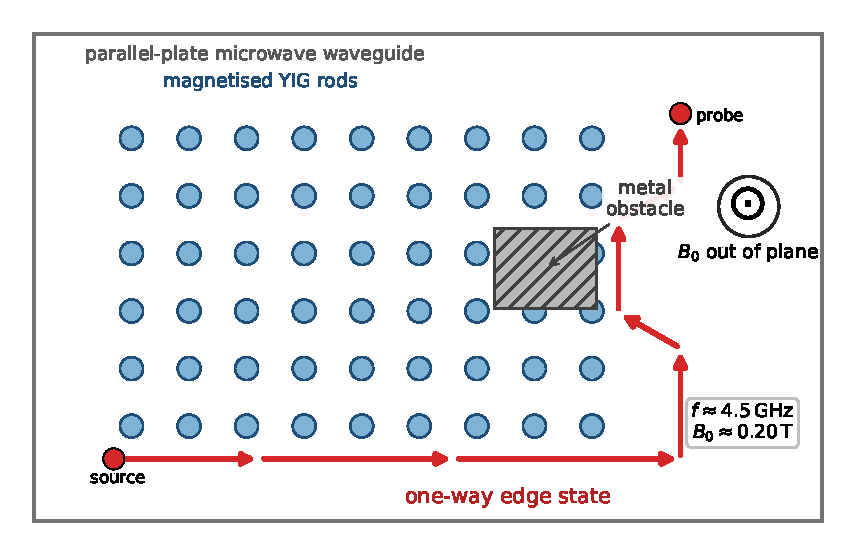
\includegraphics[width=0.88\textwidth]{figures/fig_wang_experiment_schematic.pdf}
  \caption{Schematic of the Wang et~al.\ experiment
  \cite{nature2026observation}.  A square lattice of magnetised YIG
  rods operates near $4.5$~GHz under an external bias field
  $B_0\approx 0.20$~T that breaks time-reversal symmetry.  The
  resulting gyrotropic mass, and hence the edge-state chirality, is set
  by the direction of $B_0$; the red path traces the one-way edge state routing around
  a large metallic obstacle without backscattering.}
  \label{fig:ch1-wang}
\end{figure}

\section{Why topology, and why from Maxwell?}
\label{sec:ch1-why-topology}

The preceding story can be told---and often is told---entirely in the
language of condensed-matter physics: Bloch Hamiltonians, Berry phases,
Chern numbers, bulk-boundary correspondence.  There is nothing wrong
with this; the mathematical structures are the same.  But for a book
addressed to the photonics community, and for the deepest understanding
of the physical mechanisms, we believe it is essential to derive every
topological statement directly from Maxwell's equations.

There are several reasons for this insistence.

\paragraph{The inner product is different.}
In quantum mechanics, the Hilbert-space inner product is the standard
$L^2$ integral: $\langle\psi|\phi\rangle=\int\psi^*\phi\,\dd^3 r$.
In electromagnetism, the physically correct inner product involves the
material response.  For a lossless nondispersive medium characterised by
the $6\times 6$ material matrix $\Mmat$, the electromagnetic energy
inner product is
\begin{equation}\label{eq:ch1-em-inner-product}
  \emip{\emfield_1}{\emfield_2}
  = \int \emfield_1^\dagger(\rvec)\cdot \Mmat(\rvec)\cdot
         \emfield_2(\rvec)\,\dd^3 r\,,
\end{equation}
where $\emfield = (\Efield,\Hfield)^T$ is the six-component
electromagnetic field.  Every formula for Berry connection, Berry
curvature, and Chern number must be written with respect to this inner
product, not the standard one.  Getting this wrong leads to
non-gauge-invariant expressions and incorrect topological invariants.

When the medium is dispersive---as all real magneto-optical media
are---the inner product must be further modified to incorporate the
electromagnetic energy stored in the material polarisation, leading to
the \emph{energy metric}
$\Mgmat(\omega)=\partial_\omega[\omega\Mmat(\omega)]$.  This
subtlety has no analog in the electronic problem and is easily missed
when photonic topology is derived by analogy rather than from first
principles.

\paragraph{The eigenvalue problem is generalised.}
The Maxwell normal-mode equation is not a standard eigenvalue problem
$\hat{H}\psi=E\psi$; it is a generalised eigenproblem
$\Maxop\emfield=\omega\Mmat\emfield$, with the frequency playing the
role of the eigenvalue and the material matrix appearing on the
right-hand side.  The Hermiticity (self-adjointness) that guarantees
real frequencies and orthogonal modes follows from the structure of the
Maxwell curl operator and the positivity of $\Mmat$, but the proof is
different from the quantum-mechanical case and deserves to be presented
in full.

\paragraph{Photon time reversal is bosonic.}
For electrons, the time-reversal operator satisfies $\Top^2=-1$, which
implies Kramers degeneracy and provides the symmetry protection for the
quantum spin Hall effect
\cite{kane2005sub}.  For photons, $\Top^2=+1$.  This seemingly
small algebraic difference has profound consequences: there is no
photonic Kramers theorem, and time-reversal-invariant photonic
``topological insulators'' require additional crystalline or internal
symmetries for their protection
\cite{hsieh2008topological}.  A Maxwell-first development makes this
distinction transparent from the outset.

\paragraph{Material constraints matter.}
Which materials can support topological bands?  What symmetries must be
broken, and how strong must the magneto-optical or bianisotropic
response be?  These questions can only be answered by examining the
constitutive relations directly.  A Maxwell-first approach keeps the
material physics visible at every stage, rather than hiding it behind
an effective Hamiltonian.

\section{The plan of this book}
\label{sec:ch1-plan}

This monograph develops the theory of topological photonics from the
ground up, starting from Maxwell's equations and optical energy
considerations, and building toward the full classification of
topological phases accessible to electromagnetic waves in periodic
media \cite{chen2021highlighting}.

\paragraph{Part I: Maxwell modes and optical bands.}
We begin by recasting the macroscopic Maxwell equations as a first-order
dynamical system (\chref{ch:maxwell-dynamics}), identifying the
six-component electromagnetic field and the material matrix as the
fundamental objects.  We then derive the normal-mode problem and the
electromagnetic inner product that makes it self-adjoint
(\chref{ch:normal-modes}), introduce Bloch's theorem and photonic
band structure (\chref{ch:periodic-media}), and develop the Berry
connection, Berry curvature, and Chern number for Maxwell bands
(\chref{ch:geometry-bands}).  Every formula in this part is derived from
Maxwell's equations using the correct electromagnetic inner product.

\paragraph{Part II: Chern bands and one-way waveguides.}
With the mathematical framework in place, we study the physical
mechanisms that create topological bands.  We analyse Dirac-point
degeneracies (\chref{ch:dirac-cones}), show how gyrotropic media open
topological gaps (\chref{ch:breaking-tr}), derive the one-way interface
mode at a domain wall in detail (\chref{ch:one-way-interface}), and
discuss the microwave photonic-crystal experiment that first confirmed
the prediction (\chref{ch:microwave-crystal}).  We then address the
practical problem of computing Chern numbers from numerical Maxwell
eigensolvers (\chref{ch:computing-chern}).

\paragraph{Part III: Other two-dimensional phases.}
Not all photonic topological phases require broken time-reversal
symmetry.  We discuss reciprocal designs based on pseudospin and
bianisotropy (\chref{ch:reciprocal-designs}), valley-Hall photonic
crystals (\chref{ch:valleys}), Floquet topological systems created by
temporal modulation (\chref{ch:floquet}), and one-dimensional
topological models including the photonic Su--Schrieffer--Heeger chain
(\chref{ch:one-dimension})
\cite{yang2020photonic}.

\paragraph{Part IV: Three dimensions and beyond.}
We extend the framework to three-dimensional photonic crystals with Weyl
points (\chref{ch:weyl-points}) and to synthetic dimensions created by
coupling internal degrees of freedom of resonators
(\chref{ch:synthetic-dimensions}) \cite{mancini2015observation}.

\paragraph{Part V: Imperfect, active, and nonlinear light.}
Real photonic systems have loss, gain, and nonlinearity \cite{szameit2020nonlinearity}.  We discuss
non-Hermitian topology (\chref{ch:non-hermitian}) and the emerging
frontier of nonlinear and quantum topological photonics
(\chref{ch:nonlinear-quantum})
\cite{kawabata2019symmetry}.

\paragraph{Appendices} provide supporting material on vector identities,
differential forms, numerical methods, and material-tensor conventions.

\bigskip
Throughout the book, we follow a consistent strategy: derive the key
result from Maxwell's equations first, then connect it to the
condensed-matter analogy for readers with a solid-state background, and
finally illustrate it with a concrete photonic example or experiment.
The goal is a self-contained reference that a graduate student in
photonics can read from the beginning, and that a researcher in
topological condensed matter can consult for the electromagnetic
specifics.

\section{Photonic versus electronic topology}
\label{sec:ch1-photonic-vs-electronic}

The topological ideas applied in this book were born in the study of
electron systems, but the photonic setting differs from the electronic
one in several fundamental ways.  Understanding these differences is
essential for appreciating both the power and the limitations of
topological photonics.

\subsection{Bosonic statistics and the absence of a Fermi level}
\label{sec:ch1-bosonic}

Electrons are fermions: the Pauli exclusion principle guarantees a
Fermi level that separates filled from empty states.  The topological
properties of the Chern insulator rely on this filling: the Chern
number characterises the \emph{occupied} bands below the Fermi level.

Photons are bosons: in thermal equilibrium every frequency is populated,
and there is no analog of the Fermi level.  In photonic topological
systems, the role of the Fermi level is played by the \emph{operating
frequency}, which is set by the external source.  The ``gap'' in the
photonic band structure is a frequency range with no propagating bulk
modes, and the ``edge mode'' is a propagating state at a frequency
within this gap.  The topological protection still applies---the edge
mode cannot be removed without closing the gap---but the physics of
filling and thermalisation is entirely different
\cite{ozawa2018topological}.

\subsection{Classical waves and no fundamental spin}
\label{sec:ch1-classical}

Photons have spin 1, but the spin of a photon in a medium is not a
conserved quantum number in the same way as the electron spin in a
crystal with spin-orbit coupling.  The photonic ``pseudospin'' used in
Chapter~\ref{ch:reciprocal-designs} is an emergent degree of freedom
constructed from the TE and TM polarisations, not a fundamental
symmetry.  Its protection depends on crystalline symmetry, not on
time-reversal symmetry of the fundamental Hamiltonian.

Moreover, the Maxwell equations are a classical wave equation.  All
topological effects in this book can be observed with classical light
(coherent laser beams, microwave sources) without any quantum signature.
The quantisation of edge-mode transport is a property of the wave
equation, not of the quantum statistics of the field
\cite{haldane2008possible,price2022roadmap}.

\subsection{Time-reversal symmetry and Kramers degeneracy}
\label{sec:ch1-TR-kramers}

For electrons, time reversal is an anti-unitary operator with
$\Top^2=-1$ (for half-integer spin), which implies Kramers degeneracy:
every energy level is at least doubly degenerate.  This degeneracy is
the foundation of the $\mathbb{Z}_2$ topological insulator.

For photons, $\Top^2=+1$ (because the photon spin is integer), so
there is no Kramers degeneracy.  A direct photonic analog of the
$\mathbb{Z}_2$ topological insulator requires an engineered pseudospin
with effective $\Top^2=-1$, which is possible only with specific
material symmetries (such as electromagnetic duality symmetry in
bianisotropic media).  This is why photonic topological insulators are
more constrained than their electronic counterparts, and why much of
the field has focused on Chern insulators (broken $\Top$) or
crystalline-symmetry-protected phases
\cite{ozawa2018topological,bliokh2015quantum}.

\section{Historical milestones}
\label{sec:ch1-history}

The field of topological photonics grew from two independent streams.
The first was the discovery of the integer quantum Hall effect by von
Klitzing (1980) and its topological explanation by Thouless,
Kohmoto, Nightingale, and den Nijs (1982), who showed that the Hall
conductance is proportional to an integer topological invariant---the
Chern number---of the electronic band structure
\cite{thouless1982quantized}.

The second stream was the development of photonic crystals by
Yablonovitch and John (1987), who showed that periodic dielectric
structures can have complete photonic band gaps.  The connection
between these two ideas was made by Haldane and Raghu (2008), who
demonstrated theoretically that a photonic crystal with
magneto-optical response can have bands with nonzero Chern numbers,
and therefore must support one-way edge modes
\cite{haldane2008possible}.

The experimental confirmation came in 2009, when Wang et~al.\
observed unidirectional microwave transport in a YIG photonic crystal
under an external magnetic field
\cite{nature2026observation}.  This experiment launched the field.
Since then, topological photonic effects have been demonstrated across
the electromagnetic spectrum, from microwave to optical frequencies,
using platforms ranging from coupled resonators
\cite{hafezi2013imaging} to femtosecond-laser-written waveguides
\cite{rechtsman2013photonica} to silicon photonic crystals
\cite{ma2016all,wu2017direct}.

The roadmaps by Ozawa et~al.\ (2019) and Price et~al.\ (2022) provide
comprehensive surveys of the field's development and open questions
\cite{ozawa2018topological,price2022roadmap}.

\section{The Maxwell-first philosophy}
\label{sec:ch1-maxwell-first}

This book is organised differently from most accounts of topological
photonics.  The standard approach begins with the quantum Hall effect
for electrons, derives the Chern number in a tight-binding model, and
then maps the result onto a photonic system by analogy.  This book
instead starts from Maxwell's equations and derives topology entirely
within the electromagnetic framework: the energy inner product, the
self-adjointness of the curl operator, the Berry connection on Bloch
bands, and the Chern number as an integral of the Berry curvature.

This choice is not merely pedagogical.  The electromagnetic problem
has features that differ qualitatively from the electronic one: the
material matrix $\Mmat$ is frequency-dependent and anisotropic, the
field is a six-component vector rather than a scalar, the energy inner
product involves $\Mmat$ rather than the identity, and the discrete
symmetries have different squaring properties ($\Top^2=+1$ rather
than $-1$).  An analogy-based approach risks importing results that
depend on features specific to the electronic problem, such as Kramers
degeneracy or scalar wave functions.  The Maxwell-first approach avoids
this risk entirely and reveals features---such as the role of the
dispersive energy metric---that have no direct electronic analogue
\cite{gangaraj2016berry,silveirinha2016bulk}.

\section{Open frontiers}
\label{sec:ch1-frontiers}

The field of topological photonics continues to grow rapidly.
Several frontier directions are addressed in the later parts of this
book:

Non-Hermitian topology (Chapter~\ref{ch:non-hermitian}) explores what
happens when gain and loss are introduced.  The non-Hermitian skin
effect, exceptional-point degeneracies, and the breakdown of the
conventional bulk-edge correspondence raise fundamental questions about
the meaning of topological protection in open systems
\cite{ozawa2018topological}.

Nonlinear and quantum topology (Chapter~\ref{ch:nonlinear-quantum})
asks how topological protection survives when the superposition
principle breaks down.  Solitons on topological edge modes, photon
blockade in topological cavities, and bosonic fractional quantum Hall
states of light are active areas of theoretical and experimental
investigation \cite{price2022roadmap}.

Throughout the book, we will see that the Maxwell-first framework
provides a unified language for all these directions: the same
eigenvalue equation, the same energy inner product, and the same Berry
geometry underlie the physics from microwave Chern insulators to
optical valley crystals to non-Hermitian topological lasers.

\section{Historical milestones beyond photonics}
\label{sec:ch1-milestones-beyond}

The topological ideas that underpin this book did not originate in
photonics.  They arose from a remarkable chain of discoveries in
condensed matter physics, mathematics, and quantum field theory,
spanning more than four decades.

The story begins with the integer quantum Hall effect, discovered by
von Klitzing, Dorda, and Pepper in 1980, where the Hall conductance
of a 2D electron gas in a strong magnetic field is quantised in units
of $e^2/h$ with extraordinary precision.  Thouless, Kohmoto, Nightingale,
and den Nijs (1982) showed that this quantisation is a consequence of the
Chern number of the Bloch bands---a topological invariant that cannot
change under smooth deformations of the Hamiltonian
\cite{thouless1982quantized}.

The extension to time-reversal-invariant systems came with the quantum
spin-Hall effect, predicted by Kane and Mele (2005) and independently by
Bernevig, Hughes, and Zhang (2006), and experimentally confirmed in
HgTe/CdTe quantum wells by König et~al.\ (2007).  These systems are
characterised by a $\mathbb{Z}_2$ topological invariant rather than
the Chern number, and they support helical edge modes where spin-up
and spin-down electrons propagate in opposite directions
\cite{asbth2016berry,ozawa2018topological}.

A parallel development in non-Hermitian physics began with the
observation by Bender and Boettcher (1998) that certain non-Hermitian
Hamiltonians with parity-time (PT) symmetry can have entirely real
spectra.  This insight, originally formulated in quantum mechanics,
found its most natural experimental home in photonics, where gain and
loss can be engineered with great precision
\cite{bender1998real,guo2009observation}.

The convergence of these three threads---topological band theory,
non-Hermitian physics, and photonic engineering---created the field of
topological photonics that is the subject of this book.

\section{The scope and structure of this book}
\label{sec:ch1-scope-structure}

This book develops topological photonics from Maxwell's equations.
Every topological invariant, every edge-mode derivation, and every
bulk-boundary correspondence is built from the electromagnetic
eigenvalue problem, the energy inner product, and the Bloch
decomposition---not imported from electronic band theory by analogy.

The book is organised in five parts.  Part~I
(Chapters~\ref{ch:robust-light}--\ref{ch:geometry-bands}) establishes
the mathematical framework: Maxwell's equations as a generalised
eigenvalue problem, the electromagnetic inner product and its role in
defining orthogonality and completeness, Bloch's theorem for periodic
media, and the Berry connection, Berry curvature, and Chern number as
geometric invariants of photonic bands.

Part~II (Chapters~\ref{ch:dirac-cones}--\ref{ch:computing-chern})
applies this framework to construct the first photonic topological
insulator: the gyromagnetic Chern insulator.  The key steps are the
identification of Dirac cones, the opening of a topological gap by
time-reversal-symmetry breaking, the derivation of one-way edge modes
from the bulk-edge correspondence, and the numerical computation of
Chern numbers.

Part~III (Chapters~\ref{ch:reciprocal-designs}--\ref{ch:synthetic-dimensions})
extends the topological framework to systems that preserve time-reversal
symmetry: pseudospin designs, valley photonic crystals, Floquet
topological insulators, one-dimensional chains, Weyl semimetals,
and synthetic dimensions.

Part~IV (Chapters~\ref{ch:non-hermitian}--\ref{ch:nonlinear-quantum})
treats the frontiers: non-Hermitian topology, topological lasers,
nonlinear effects, and quantum topological photonics.

The four appendices provide the mathematical tools: vector identities
and functional analysis, differential forms and Chern classes,
numerical algorithms, and material tensor conventions.

The reader is assumed to be familiar with classical electrodynamics
at the level of Jackson or Griffiths, and with quantum mechanics at
the level of Sakurai.  No prior knowledge of topology or differential
geometry is required: these subjects are developed from scratch as
needed \cite{ozawa2018topological}.

\section{Why photonic topology differs from electronic topology}

Why study topology in photonics rather than simply importing results
from electronic band theory?  The answer touches on both fundamental
physics and practical engineering.

\subsection{Bosons versus fermions}
\label{sec:ch1-bosons-vs-fermions}

Electrons are fermions with half-integer spin, obeying the Pauli
exclusion principle and filling bands up to the Fermi energy.  Photons
are bosons with integer spin, obeying Bose--Einstein statistics and
occupying any number of modes simultaneously.  This distinction has
deep consequences for topology:

In electronic systems, the Fermi energy naturally defines which bands
are ``occupied'' and which are ``empty,'' providing a sharp boundary
for computing topological invariants.  In photonics, there is no Fermi
energy; all bands below a gap can be excited.  The photonic Chern
number must therefore be defined as a sum over all bands below the gap,
weighted by the electromagnetic energy inner product
(Chapter~\ref{ch:normal-modes})---a structure that has no direct
electronic analog \cite{gangaraj2016berry,silveirinha2016bulk}.

Furthermore, the spin-statistics theorem guarantees that electronic
topological insulators with time-reversal symmetry are classified by
$\mathbb{Z}_2$ invariants, protected by Kramers degeneracy.  Photons
do not have Kramers degeneracy (they are spin-1 bosons), so the
$\mathbb{Z}_2$ classification requires an additional symmetry---either
electromagnetic duality or crystalline symmetry---to protect the
pseudospin structure
\cite{bliokh2015quantum,mario2016microsoft}.

\subsection{Maxwell versus Schrödinger}
\label{sec:ch1-maxwell-vs-schrodinger}

The Schrödinger equation is a scalar first-order equation in time,
while Maxwell's equations form a vector first-order system.  The
vectorial nature of light means that the Berry connection is a matrix
connection on a vector bundle, not merely a U(1) connection on a
line bundle.  This enriches the topology: photonic bands can carry
non-Abelian Berry phases and support topological invariants (such as
the Euler class) that have no scalar analog
\cite{ozawa2018topological,price2022roadmap}.

The first-order structure of Maxwell's equations also means that the
``Hamiltonian'' $\Maxop$ is not bounded below: unlike the Schrödinger
Hamiltonian, the Maxwell operator has both positive and negative
frequency eigenvalues.  The positive-definiteness of the material
tensor $\Mmat$ plays the role of the positive-definite mass in
quantum mechanics, ensuring that the electromagnetic inner product
is positive-definite and that the Berry connection is well-defined
(Chapter~\ref{ch:maxwell-dynamics}).

\section{Why the Maxwell-first route matters}
\label{sec:ch1-maxwell-first-route}

It is tempting to introduce topological photonics by first describing
electronic topological insulators and then replacing an electron wave
function by an electromagnetic field.  That route is historically
understandable, because many of the words---Berry curvature, Chern
number, band gap, edge state---entered photonics from condensed-matter
physics.  But it hides the essential difference between the two
problems.  An electron band in a crystal is an eigenproblem for a
Schrödinger operator acting on a scalar or spinor wave function.  An
optical band is an eigenproblem for Maxwell's equations acting on a
six-component field $(\Efield,\Hfield)$, constrained by divergence
conditions and weighted by the electromagnetic energy stored in a
material medium.

The distinction is not cosmetic.  The inner product that makes a
lossless Maxwell operator self-adjoint is not the ordinary
$L^2$ product.  In a nondispersive medium it is
\begin{equation}\label{eq:ch1-energy-product-preview}
  \langle \Psi_1,\Psi_2\rangle_{\Mmat}
  = \int \bigl(\Efield_1^*\cdot\varepsilon\Efield_2
       + \Hfield_1^*\cdot\mu\Hfield_2\bigr)\,\dd^3 r,
  \qquad \Psi=(\Efield,\Hfield)^T,
\end{equation}
and in a dispersive medium it is replaced by the Brillouin energy
metric involving $\partial_\omega(\omega\Mmat)$.  Berry phases and
Chern numbers of photonic bands are therefore geometric phases of
\emph{energy-normalised Maxwell modes}, not phases of arbitrary field
amplitudes.  This is the reason Chapters~\ref{ch:maxwell-dynamics}
through~\ref{ch:geometry-bands} build the subject from Maxwell's
equations rather than importing the electronic formalism at the start
\cite{gangaraj2016berry,silveirinha2016bulk,haldane2008possible}.

The Maxwell-first route also prevents a common misunderstanding about
``spin'' in photonics.  Photons have helicity, polarisation, and
orbital angular momentum, but a reciprocal dielectric crystal does not
possess the Kramers degeneracy of a spin-$1/2$ electron unless an
additional pseudo-spin structure is engineered.  Bianisotropic
metamaterials, coupled resonator arrays, and valley crystals all
construct such structures in different ways
\cite{khanikaev2013photonic,hafezi2013imaging,mit2026pdf}.  A monograph
that begins with electronic spin-orbit coupling would make these
photonic designs seem like analogues.  A Maxwell-first monograph shows
instead what they really are: carefully designed degeneracies and
symmetries of the electromagnetic normal-mode problem.

\section{The organising question of the book}
\label{sec:ch1-organising-question}

The central question of this book can be stated in one sentence:
\emph{when can Maxwell's equations force light to move along a boundary
without backscattering?}  The answer has several layers.

At the most local level, a boundary mode is an evanescent solution of
Maxwell's equations whose field decays away from an interface.  At the
band-theoretic level, it appears in a frequency gap separating two
bulk continua.  At the topological level, it is required when the two
bulk media on the two sides of the interface cannot be continuously
deformed into each other without closing the gap.  This final statement
is the bulk-boundary principle.  It is simple to say, but for photons it
is not a postulate: it has to be tied to the Maxwell operator, the
energy inner product, material dispersion, and electromagnetic boundary
conditions.

The first experimental demonstrations made this question concrete.  The
microwave photonic crystal experiment of Wang et~al.\ showed a chiral
edge channel in a gyromagnetic crystal biased by a static magnetic field
\cite{wang2009observation}.  The helical waveguide experiment of
Rechtsman et~al.\ showed that longitudinal modulation can create an
effective Floquet gauge field for light \cite{rechtsman2013photonic}.
The coupled-resonator experiments showed that synthetic magnetic flux
can be engineered on a chip \cite{hafezi2013imaging}.  These platforms
look very different in the laboratory, but all answer the same Maxwell
question: what does a material or modulation do to the geometry of the
normal modes?

The chapters that follow return to this question repeatedly.  The
answer is first a self-adjoint Maxwell eigenproblem, then a Bloch bundle,
then a Berry curvature, then an integer Chern number, then an edge mode.
The later chapters complicate the setting---reciprocity, valleys,
Floquet driving, three dimensions, synthetic dimensions, gain and loss,
nonlinearity, and quantum light---but the path remains the same: start
from the fields and ask what structure Maxwell's equations allow.

\section*{Exercises}

\begin{exercise}
  A single-mode silicon-on-insulator waveguide ($n_1=3.48$,
  $n_2=1.44$, core width $450\;\mathrm{nm}$, operating wavelength
  $1550\;\mathrm{nm}$) has sidewall roughness with
  $\sigma=2\;\mathrm{nm}$ and $L_c=50\;\mathrm{nm}$.  Using the
  scaling in \eqnref{eq:ch1-roughness-loss}, estimate the order of
  magnitude of the backscattering-limited propagation length and compare
  it to a typical ring-resonator circumference of
  $100\;\mu\mathrm{m}$.
\end{exercise}

\begin{exercise}
  In a Faraday isolator, the polarisation rotation angle in a medium of
  length $L$ with Verdet constant $V$ in a magnetic field $B$ is
  $\theta_F = VBL$.  For a bismuth iron garnet film at
  $\lambda=1550\;\mathrm{nm}$ with $V\approx 10^3\;\mathrm{deg\,cm}^{-1}\mathrm{T}^{-1}$, estimate the film thickness and field
  needed for a $45^{\circ}$ rotation.  Why is this approach difficult
  to miniaturise to on-chip waveguide scales?
\end{exercise}

\begin{exercise}
  Time reversal in electromagnetism sends $(\Efield,\Hfield)\to
  (\Efield,-\Hfield)$.  Show that this maps a plane-wave mode
  $\sim\ee^{\ii(\kvec\cdot\rvec-\omega t)}$ to one with
  $\kvec\to-\kvec$ and the same frequency, and that the dispersion
  relation of a lossless reciprocal waveguide therefore satisfies
  $\omega(\kvec)=\omega(-\kvec)$.
\end{exercise}


\chapter{Maxwell Equations as Dynamics}
\label{ch:maxwell-dynamics}
% ======================================================================
%  Chapter 2 — Maxwell Equations as Dynamics
% ======================================================================

\section{The macroscopic Maxwell equations}
\label{sec:ch2-macroscopic-maxwell}

We work throughout this book with the \emph{macroscopic} Maxwell
equations, in which the response of bound charges and currents is
encoded in the constitutive fields $\Dfield$ and $\Bfield$
\cite{press2026photonic}.  In the
absence of free charges and currents, these equations read
\begin{subequations}\label{eq:ch2-maxwell-time}
\begin{align}
  \nabla\times\Efield(\rvec,t) &= -\pderiv{\Bfield(\rvec,t)}{t}\,,
  \label{eq:ch2-faraday}\\[4pt]
  \nabla\times\Hfield(\rvec,t) &= \phantom{-}\pderiv{\Dfield(\rvec,t)}{t}\,,
  \label{eq:ch2-ampere}\\[4pt]
  \nabla\cdot\Dfield(\rvec,t)  &= 0\,,
  \label{eq:ch2-gauss-e}\\[4pt]
  \nabla\cdot\Bfield(\rvec,t)  &= 0\,.
  \label{eq:ch2-gauss-m}
\end{align}
\end{subequations}
Here $\Efield$ and $\Hfield$ are the electric and magnetic field
intensities, while $\Dfield$ and $\Bfield$ are the electric
displacement and magnetic flux density.  SI units are used throughout.

\begin{remark}
Equations \eqref{eq:ch2-gauss-e} and \eqref{eq:ch2-gauss-m} are not
independent of the curl equations.  Taking the divergence of
\eqref{eq:ch2-faraday} gives $\partial_t(\nabla\cdot\Bfield)=0$, so if
$\nabla\cdot\Bfield=0$ is satisfied at one time it holds for all time;
similarly for $\nabla\cdot\Dfield$.  The divergence conditions are
therefore constraints on the initial data, not additional dynamical
equations.  We will return to this point in \chref{ch:normal-modes}
when we discuss the completeness of the normal-mode expansion.
\end{remark}

\section{Constitutive relations}
\label{sec:ch2-constitutive}

The Maxwell equations become a closed dynamical system only when
supplemented by \emph{constitutive relations} that express $\Dfield$
and $\Bfield$ in terms of $\Efield$ and $\Hfield$ \cite{khanikaev2013photonic}.  We consider linear
media and work in the frequency domain, writing time-harmonic fields as
$\Efield(\rvec,t)=\real[\Efield(\rvec)\ee^{-\ii\omega t}]$ (and
similarly for $\Hfield$, $\Dfield$, $\Bfield$).

\subsection{Isotropic media}
\label{sec:ch2-isotropic}

The simplest case is a local, isotropic, nondispersive dielectric:
\begin{equation}\label{eq:ch2-isotropic}
  \Dfield = \varepsilon_0\,\varepsilon(\rvec)\,\Efield\,,
  \qquad
  \Bfield = \mu_0\,\mu(\rvec)\,\Hfield\,,
\end{equation}
where $\varepsilon(\rvec)$ and $\mu(\rvec)$ are the relative
permittivity and permeability.  Most photonic-crystal literature begins
here, with $\mu=1$ (nonmagnetic media) and $\varepsilon(\rvec)$ varying
periodically.  For topological photonics, however, we will need to go
beyond this simplest setting.

\subsection{Anisotropic media}
\label{sec:ch2-anisotropic}

In an anisotropic crystal, the permittivity and permeability become
$3\times 3$ tensors:
\begin{equation}\label{eq:ch2-anisotropic}
  D_i = \varepsilon_0\,\varepsilon_{ij}(\rvec)\,E_j\,,
  \qquad
  B_i = \mu_0\,\mu_{ij}(\rvec)\,H_j\,,
\end{equation}
with summation over repeated indices.  The tensors $\epst$ and $\mut$
are Hermitian ($\varepsilon_{ij}=\varepsilon_{ji}^*$,
$\mu_{ij}=\mu_{ji}^*$) for lossless media at real frequencies.

A particularly important special case is the \emph{gyrotropic}
medium, in which an applied magnetic bias $\Bfield_0 = B_0\hat{z}$
induces off-diagonal imaginary components.  For a ferrite magnetised
along $z$, the permeability tensor takes the form
\begin{equation}\label{eq:ch2-gyrotropic-mu}
  \mut =
  \begin{pmatrix}
    \mu_{\perp} & -\ii\kappa & 0 \\
    \ii\kappa & \mu_{\perp} & 0 \\
    0 & 0 & \mu_z
  \end{pmatrix},
\end{equation}
where $\mu_\perp$, $\kappa$, and $\mu_z$ are real parameters that
depend on frequency and the magnetisation.  The antisymmetric
off-diagonal element $\kappa$ is the \emph{gyrotropic parameter}; it
vanishes when $B_0=0$ and breaks time-reversal symmetry when
$\kappa\neq 0$.

\begin{remark}
The Hermiticity of $\mut$ is manifest:
$\mu_{12}=-\ii\kappa$ and $\mu_{21}=\ii\kappa=\mu_{12}^*$ for real
$\kappa$.  The eigenvalues of $\mut$ are $\mu_\perp\pm\kappa$ and
$\mu_z$; positivity of the energy requires
$\mu_\perp>|\kappa|>0$ and $\mu_z>0$.
\end{remark}

\subsection{The bianisotropic material matrix}
\label{sec:ch2-bianisotropic}

The most general linear local constitutive relation couples all four
fields:
\begin{equation}\label{eq:ch2-bianisotropic}
  \begin{pmatrix} \Dfield \\ \Bfield \end{pmatrix}
  =
  \begin{pmatrix}
    \varepsilon_0\,\epst & \clight^{-1}\,\xit \\[4pt]
    \clight^{-1}\,\zetat & \mu_0\,\mut
  \end{pmatrix}
  \begin{pmatrix} \Efield \\ \Hfield \end{pmatrix}
  \;\equiv\;
  \Mmat(\rvec,\omega)
  \begin{pmatrix} \Efield \\ \Hfield \end{pmatrix}.
\end{equation}
Here $\xit$ and $\zetat$ are the magneto-electric coupling tensors, and
$\Mmat$ is the $6\times 6$ \emph{material matrix}.

\begin{definition}[Lossless medium]
  \label{def:ch2-lossless}
  A linear medium is \emph{lossless at frequency~$\omega$} if and only
  if the material matrix is Hermitian:
  \begin{equation}\label{eq:ch2-lossless}
    \Mmat(\rvec,\omega) = \Mmat^\dagger(\rvec,\omega).
  \end{equation}
  For the individual blocks, this requires $\epst=\epst^\dagger$,
  $\mut=\mut^\dagger$, and $\zetat=\xit^\dagger$.
\end{definition}

We will see in \secref{sec:ch2-poynting} that condition
\eqref{eq:ch2-lossless} is precisely the requirement that the
time-averaged electromagnetic energy is conserved.

\begin{definition}[Positive energy]
  \label{def:ch2-positive-energy}
  A lossless medium has \emph{positive electromagnetic energy} if
  $\Mmat(\rvec,\omega)$ is positive definite for all $\rvec$ in the
  medium and for the frequencies of interest.  This means
  $\emfield^\dagger\Mmat\,\emfield>0$ for every nonzero six-component
  field $\emfield=(\Efield,\Hfield)^T$.
\end{definition}

The positive-energy condition is the electromagnetic analog of the
positive-definite kinetic energy in mechanics.  It will be essential for
the Hermiticity of the normal-mode problem
(\chref{ch:normal-modes}).

\section{The six-component first-order form}
\label{sec:ch2-first-order}

Following Haldane and Raghu, we now rewrite Maxwell's equations as a
first-order eigenvalue problem in the frequency domain.

\subsection{Harmonic fields and the curl matrix}
\label{sec:ch2-curl-matrix}

For time-harmonic fields $\sim\ee^{-\ii\omega t}$, the curl equations
\eqref{eq:ch2-faraday}--\eqref{eq:ch2-ampere} become
\begin{subequations}\label{eq:ch2-maxwell-freq}
\begin{align}
  \nabla\times\Efield &= \ii\omega\,\Bfield\,,
  \label{eq:ch2-faraday-freq}\\
  \nabla\times\Hfield &= -\ii\omega\,\Dfield\,.
  \label{eq:ch2-ampere-freq}
\end{align}
\end{subequations}
(We adopt the engineering convention $\ee^{-\ii\omega t}$ with $\omega>0$
for forward-propagating modes throughout.)

Define the six-component electromagnetic field
\begin{equation}\label{eq:ch2-sixfield}
  \emfield(\rvec)
  = \begin{pmatrix} \Efield(\rvec) \\[2pt] \Hfield(\rvec) \end{pmatrix}
\end{equation}
and the $6\times 6$ Maxwell curl operator
\begin{equation}\label{eq:ch2-maxop}
  \Maxop
  \;\equiv\;
  \begin{pmatrix}
    \mathbf{0} & \ii\,\nabla\times \\[2pt]
    -\ii\,\nabla\times & \mathbf{0}
  \end{pmatrix}.
\end{equation}
Then the pair of curl equations collapses into the single matrix
equation
\begin{equation}\label{eq:ch2-maxwell-matrix}
  \boxed{%
  \Maxop\,\emfield(\rvec)
  = \omega\,\Mmat(\rvec,\omega)\,\emfield(\rvec).}
\end{equation}
This is the fundamental \emph{Maxwell eigenvalue equation} in
first-order form.  It will serve as the starting point for normal modes
(\chref{ch:normal-modes}), Bloch bands
(\chref{ch:periodic-media}), and Berry geometry
(\chref{ch:geometry-bands}).

\begin{figure}[!t]
  \centering
  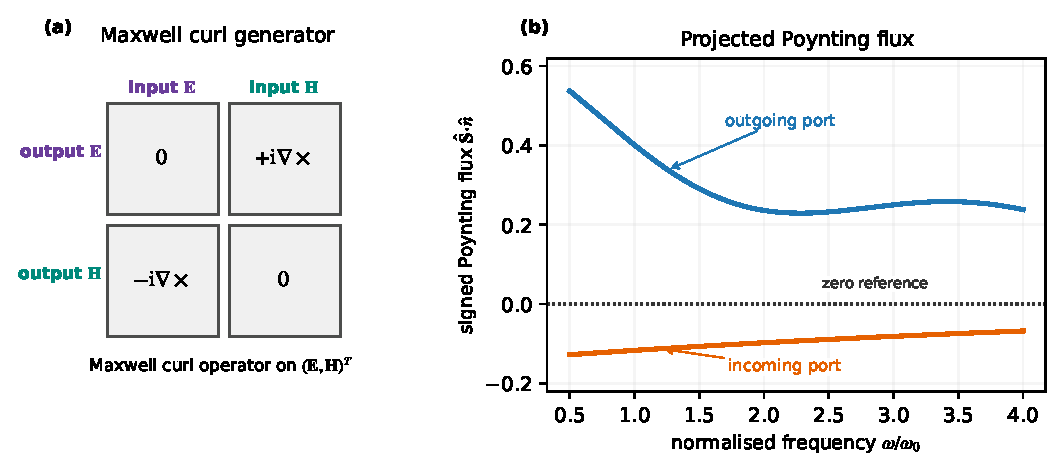
\includegraphics[width=0.92\textwidth]{figures/fig_ch02_operator_structure_step199.pdf}
  \caption{Structure of the Maxwell curl operator $\Maxop$ and energy flux.
  \textbf{(a)}~Block structure of the time generator: the $6\times 6$
  operator $\Maxop$ defined in \eqref{eq:ch2-maxop} has vanishing diagonal
  blocks (no direct $\Efield$--$\Efield$ or $\Hfield$--$\Hfield$ coupling)
  and antisymmetric off-diagonal curl blocks ($+\ii\nabla\times$ couples
  $\Hfield$ into the $\Efield$ equation; $-\ii\nabla\times$ couples
  $\Efield$ into the $\Hfield$ equation), consistent with the
  $e^{-\ii\omega t}$ time convention used throughout this book.
  \textbf{(b)}~Signed normal Poynting flux $\hat{\mathbf{S}}\cdot\hat{n}$
  for a guided mode at a port boundary, illustrating energy flow into
  (incoming port) and out of (outgoing port) the computational domain.
  The zero reference line marks the interface between forward and
  backward flux.}
  \label{fig:ch02-operator-structure}
\end{figure}


\begin{remark}
The off-diagonal structure of $\Maxop$ in
\eqref{eq:ch2-maxop}---coupling $\Efield$ to $\Hfield$ through the
curl---is a reflection of the fact that electromagnetic waves are
intrinsically coupled electric and magnetic phenomena.  This structure
is preserved under all linear constitutive extensions and is the origin
of the spin-1 character of photons.
\end{remark}

\subsection{Momentum representation}
\label{sec:ch2-momentum}

For a spatially homogeneous medium, or for the cell-periodic part of a
Bloch mode in a periodic medium, we can replace $\nabla$ by
$\ii\kvec$ to obtain the momentum-space curl operator
\begin{equation}\label{eq:ch2-maxop-k}
  \Maxop(\kvec)
  =
  \begin{pmatrix}
    \mathbf{0} & -\kvec\times \\[2pt]
    \kvec\times & \mathbf{0}
  \end{pmatrix},
\end{equation}
where $(\kvec\times)_{ij}=-\epsilon_{ijk}k_k$ is the $3\times 3$
antisymmetric matrix associated with the cross product.  Explicitly, for
$\kvec=(k_x,k_y,k_z)$:
\begin{equation}\label{eq:ch2-cross-matrix}
  \kvec\times
  =
  \begin{pmatrix}
    0 & -k_z & k_y \\
    k_z & 0 & -k_x \\
    -k_y & k_x & 0
  \end{pmatrix}.
\end{equation}
It is straightforward to verify that $\Maxop(\kvec)$ is Hermitian:
$\Maxop(\kvec)=\Maxop^\dagger(\kvec)$, since the cross-product matrix
is real and antisymmetric, so $(\kvec\times)^T=-\kvec\times$, and the
block off-diagonal structure with the signs in \eqref{eq:ch2-maxop-k}
makes the full $6\times6$ matrix symmetric.

\begin{remark}[Spin-1 matrices]
Haldane and Raghu write the curl operator as $A=-\ii J^a\nabla_a$,
where $J^a$ are $6\times6$ matrices built from the spin-1
representation of $\mathrm{SO}(3)$.  In components,
$(L^a)_{bc}=\ii\epsilon_{abc}$ are the $3\times3$ generators of
rotations, and $J^a$ is the block off-diagonal matrix
$J^a = \bigl(\begin{smallmatrix}0 & \ii L^a \\ -\ii L^a &
0\end{smallmatrix}\bigr)$.  This representation makes the rotational
symmetry of the Maxwell operator manifest and connects directly to the
spin-1 nature of the photon.
\end{remark}


\section{Electromagnetic energy}
\label{sec:ch2-energy}

The energy carried by electromagnetic fields is central to everything
that follows.  The correct inner product for the Maxwell eigenvalue
problem is built from the electromagnetic energy, so we derive the
Poynting theorem in detail.

\subsection{Poynting's theorem in the time domain}
\label{sec:ch2-poynting-time}

We start from the standard derivation.  Take the dot product of
\eqref{eq:ch2-faraday} with $\Hfield$ and of \eqref{eq:ch2-ampere}
with $\Efield$:
\begin{align}
  \Hfield\cdot(\nabla\times\Efield)
  &= -\Hfield\cdot\pderiv{\Bfield}{t}\,,
  \label{eq:ch2-poynting-step1}\\
  \Efield\cdot(\nabla\times\Hfield)
  &= \Efield\cdot\pderiv{\Dfield}{t}\,.
  \label{eq:ch2-poynting-step2}
\end{align}
Subtract \eqref{eq:ch2-poynting-step1} from
\eqref{eq:ch2-poynting-step2} and use the vector identity
$\nabla\cdot(\Efield\times\Hfield)
 =\Hfield\cdot(\nabla\times\Efield)
 -\Efield\cdot(\nabla\times\Hfield)$
to obtain
\begin{equation}\label{eq:ch2-poynting-differential}
  \nabla\cdot(\Efield\times\Hfield)
  + \Efield\cdot\pderiv{\Dfield}{t}
  + \Hfield\cdot\pderiv{\Bfield}{t}
  = 0\,.
\end{equation}
Define the Poynting vector and the instantaneous energy density:
\begin{equation}\label{eq:ch2-poynting-defs}
  \Sfield(\rvec,t) = \Efield\times\Hfield\,,
  \qquad
  u(\rvec,t) = \frac{1}{2}\bigl(
    \Efield\cdot\Dfield + \Hfield\cdot\Bfield
  \bigr).
\end{equation}
For nondispersive media with $\Dfield=\varepsilon_0\epst\Efield$ and \cite{silveirinha2016bulk}
$\Bfield=\mu_0\mut\Hfield$, the terms
$\Efield\cdot\partial_t\Dfield$ and $\Hfield\cdot\partial_t\Bfield$
equal $\partial_t u$ when $\epst$ and $\mut$ are
time-independent.\footnote{%
  For dispersive media the identification
  $\Efield\cdot\partial_t\Dfield=\partial_t(\frac12\Efield\cdot\Dfield)$
  does not hold in general; see \secref{sec:ch2-dispersive-energy}.}
Poynting's theorem then takes the conservation-law form
\begin{equation}\label{eq:ch2-poynting-conservation}
  \boxed{%
  \pderiv{u}{t} + \nabla\cdot\Sfield = 0\,.}
\end{equation}
Integrating over any volume $V$ bounded by a surface $\partial V$:
\begin{equation}
  \tderiv{}{t}\int_V u\,\dd^3r
  = -\oint_{\partial V}\Sfield\cdot\hat{n}\,\dd A\,.
\end{equation}
Energy stored in $V$ changes only through the Poynting flux across the
boundary.  In a lossless medium, energy is neither created nor
destroyed; the field energy is exactly accounted for by the flux.

\subsection{Time-averaged energy for harmonic fields}
\label{sec:ch2-energy-harmonic}

For monochromatic fields
$\Efield(\rvec,t)=\real[\Efield(\rvec)\ee^{-\ii\omega t}]$, the
time-averaged Poynting vector and energy density are
\begin{equation}\label{eq:ch2-time-avg}
  \langle\Sfield\rangle
  = \frac{1}{2}\real(\Efield\times\Hfield^*)\,,
  \qquad
  \langle u\rangle
  = \frac{1}{4}\real\bigl(
    \Efield^*\cdot\Dfield + \Hfield^*\cdot\Bfield
  \bigr).
\end{equation}

Using the bianisotropic constitutive relation \eqref{eq:ch2-bianisotropic},
the time-averaged energy density can be written compactly in terms of
the six-component field as
\begin{equation}\label{eq:ch2-energy-sixfield}
  \langle u\rangle
  = \frac{1}{4}\,\emfield^\dagger(\rvec)\cdot\Mmat(\rvec,\omega)
    \cdot\emfield(\rvec)\,.
\end{equation}
When $\Mmat$ is Hermitian and positive definite, $\langle u\rangle>0$
for any nonzero $\emfield$.  This is the physical content of
Definitions~\ref{def:ch2-lossless} and \ref{def:ch2-positive-energy}.

\subsection{Energy in dispersive media}
\label{sec:ch2-dispersive-energy}

All real materials are dispersive: the material matrix
$\Mmat(\rvec,\omega)$ depends on frequency.  In a dispersive
medium, the time-averaged energy density of a \emph{quasi-monochromatic}
wave packet (bandwidth $\Delta\omega\ll\omega$) is given by the
Brillouin formula
\begin{equation}\label{eq:ch2-brillouin-energy}
  \langle u\rangle_{\mathrm{disp}}
  = \frac{1}{4}\,\emfield^\dagger(\rvec)\cdot
  \pderiv{}{\omega}\bigl[\omega\,\Mmat(\rvec,\omega)\bigr]
  \cdot\emfield(\rvec)
  = \frac{1}{4}\,\emfield^\dagger\cdot\Mgmat(\omega)\cdot\emfield\,,
\end{equation}
where we define the \emph{energy metric}
\begin{equation}\label{eq:ch2-energy-metric}
  \boxed{%
  \Mgmat(\rvec,\omega)
  \;\equiv\;
  \pderiv{}{\omega}\bigl[\omega\,\Mmat(\rvec,\omega)\bigr]
  = \Mmat + \omega\,\pderiv{\Mmat}{\omega}\,.}
\end{equation}

\begin{remark}
In the nondispersive limit ($\partial\Mmat/\partial\omega=0$), the
energy metric reduces to $\Mgmat=\Mmat$, and
\eqref{eq:ch2-brillouin-energy} reduces to
\eqref{eq:ch2-energy-sixfield}.
\end{remark}

The requirement that the electromagnetic energy is positive
($\langle u\rangle_\mathrm{disp}>0$ for all nonzero $\emfield$)
translates into the \emph{stability condition}:
\begin{equation}\label{eq:ch2-stability}
  \Mgmat(\rvec,\omega)\;\text{is positive definite}
\end{equation}
at every physical eigenfrequency.  This condition was emphasised by
Haldane and Raghu as the correct generalisation of the positive-energy
requirement for dispersive Maxwell systems, and it will play a crucial
role in the inner product of \chref{ch:normal-modes}.

\paragraph{Derivation of the Brillouin formula.}
The result \eqref{eq:ch2-brillouin-energy} can be derived by
considering a wave packet
$\Efield(\rvec,t)=\real[\hat\Efield(\rvec)\,a(t)\,\ee^{-\ii\omega_0 t}]$
with slowly varying envelope $a(t)$ centred at frequency $\omega_0$.
The constitutive relation in the time domain involves a convolution:
$\Dfield(\rvec,t)=\int_{-\infty}^{t}\varepsilon_0\epst(\rvec,t-t')
\Efield(\rvec,t')\,\dd t'$.  For a narrow-band envelope, one expands
the frequency-domain susceptibility to first order around $\omega_0$:
\begin{equation}
  \omega\,\varepsilon_{ij}(\omega)
  \approx \omega_0\,\varepsilon_{ij}(\omega_0)
  + (\omega-\omega_0)\,
  \pderiv{}{\omega}\bigl[\omega\,\varepsilon_{ij}\bigr]
  \Big|_{\omega_0}.
\end{equation}
Substituting into the Poynting identity and time-averaging over the
carrier oscillation yields \eqref{eq:ch2-brillouin-energy} for the
$\epst$ block; the $\mut$, $\xit$, and $\zetat$ blocks follow
identically, giving the full $6\times 6$ result.

\section{Poynting's theorem for harmonic fields}
\label{sec:ch2-poynting}

We now derive the frequency-domain version of Poynting's theorem and
show that it encodes the losslessness condition directly.

Take the complex conjugate of \eqref{eq:ch2-faraday-freq}:
$\nabla\times\Efield^*=-\ii\omega\Bfield^*$.  Form
$\Hfield\cdot(\nabla\times\Efield^*)-\Efield^*\cdot(\nabla\times\Hfield)$
and use the identity
$\nabla\cdot(\Efield^*\times\Hfield)
=\Hfield\cdot(\nabla\times\Efield^*)
-\Efield^*\cdot(\nabla\times\Hfield)$:
\begin{equation}\label{eq:ch2-complex-poynting}
  \nabla\cdot(\Efield^*\times\Hfield)
  = -\ii\omega\bigl(
    \Hfield\cdot\Bfield^* - \Efield^*\cdot\Dfield
  \bigr).
\end{equation}
Using the constitutive relation in six-component form, the right-hand
side becomes
\begin{equation}
  -\ii\omega\,\emfield^\dagger
  \begin{pmatrix}
    -\vac\epst & -\clight^{-1}\xit \\
    \muvac\mut^\dagger & \clight^{-1}\zetat^\dagger
  \end{pmatrix}
  \emfield\,.
\end{equation}
Taking the imaginary part:
\begin{equation}\label{eq:ch2-loss-condition}
  \frac{1}{2}\nabla\cdot\real(\Efield^*\times\Hfield)
  = -\frac{\omega}{2}\,\emfield^\dagger\cdot
    \frac{\Mmat-\Mmat^\dagger}{2\ii}\cdot\emfield\,.
\end{equation}
The left-hand side is the divergence of the time-averaged Poynting
vector.  If $\Mmat=\Mmat^\dagger$, the right-hand side vanishes
identically: the divergence of the Poynting flux is zero everywhere,
confirming that no energy is absorbed or generated.

\begin{proposition}[Losslessness from Hermiticity]
  \label{prop:ch2-lossless}
  A linear medium is lossless (zero absorption and gain at frequency
  $\omega$) if and only if $\Mmat(\rvec,\omega)=\Mmat^\dagger(\rvec,\omega)$.
\end{proposition}

\section{Symmetries of the Maxwell system}
\label{sec:ch2-symmetries}

The topological classification of photonic bands depends critically on
which discrete symmetries the Maxwell system possesses \cite{ozawa2018topological}.  We now derive
the three most important ones from the structure of $\Mmat$ and
$\Maxop$.

\subsection{Time reversal}
\label{sec:ch2-time-reversal}

The microscopic Maxwell equations are invariant under time reversal
$t\to -t$.  In the macroscopic theory, time reversal acts on the fields
as
\begin{equation}\label{eq:ch2-TR-fields}
  \Top:\;
  \Efield(\rvec,t)\to\Efield(\rvec,-t)\,,\quad
  \Hfield(\rvec,t)\to-\Hfield(\rvec,-t)\,.
\end{equation}
The sign difference arises because $\Efield$ is a polar vector
(unchanged under $t\to -t$) while $\Hfield$ is an axial vector
proportional to a current ($\Jfield\propto\dd q/\dd t$ changes sign).

For a time-harmonic field $\emfield\ee^{-\ii\omega t}$, the
time-reversal operation becomes complex conjugation combined with a sign
flip on the magnetic component:
\begin{equation}\label{eq:ch2-TR-harmonic}
  \Top:\;
  \begin{pmatrix}\Efield\\\Hfield\end{pmatrix}
  \;\mapsto\;
  \begin{pmatrix}\Efield^*\\-\Hfield^*\end{pmatrix},
  \qquad
  \kvec\to-\kvec\,,\quad \omega\to\omega\,.
\end{equation}
We can represent this as $\Top=\mathcal{K}\,\sigma_z$, where
$\mathcal{K}$ is complex conjugation and
$\sigma_z=\diag(\mathbf{I}_3,-\mathbf{I}_3)$ acts on the
electric/magnetic block structure.

\paragraph{Bosonic time reversal: $\Top^2=+1$.}
Applying $\Top$ twice:
$\Top^2\emfield = \mathcal{K}\sigma_z\mathcal{K}\sigma_z\emfield
= \sigma_z^2\emfield = \emfield$.
Thus $\Top^2=+\mathbf{1}$ for photons.  This is fundamentally different
from the electronic case, where $\Top^2=-\mathbf{1}$ due to half-integer
spin.

\begin{proposition}[Absence of photonic Kramers degeneracy]
  \label{prop:ch2-no-kramers}
  Since $\Top^2=+1$ for photons, there is no Kramers theorem for
  electromagnetic modes.  Time-reversal symmetry alone does not
  guarantee twofold degeneracy at time-reversal-invariant momenta.
  Consequently, the $\mathbb{Z}_2$ topological classification of the
  quantum spin Hall effect does not directly apply to photonic systems.
\end{proposition}

\paragraph{Condition on the material matrix.}
The Maxwell eigenvalue equation is time-reversal invariant if and only
if, for every solution $\emfield$ at $(\omega,\kvec)$, the
time-reversed field $\Top\emfield$ is also a solution at
$(\omega,-\kvec)$.  Substituting into \eqref{eq:ch2-maxwell-matrix} and
using the explicit form of $\Top$, one finds that this requires
\begin{equation}\label{eq:ch2-TR-condition}
  \sigma_z\,\Mmat^*(\omega)\,\sigma_z = \Mmat(\omega)\,.
\end{equation}
In block form, this reads
\begin{equation}\label{eq:ch2-TR-blocks}
  \epst^* = \epst\,,\quad
  \mut^* = \mut\,,\quad
  \xit^* = -\xit\,,\quad
  \zetat^* = -\zetat\,.
\end{equation}
For the gyrotropic permeability of \eqref{eq:ch2-gyrotropic-mu},
condition \eqref{eq:ch2-TR-blocks} requires $\kappa=0$.  A nonzero
gyrotropic parameter therefore \emph{breaks time-reversal symmetry}.

\subsection{Reciprocity}
\label{sec:ch2-reciprocity}

A medium is \emph{reciprocal} if the Lorentz reciprocity relation holds:
for any two solutions $\emfield_a$ and $\emfield_b$ of the Maxwell
equations at the same frequency,
\begin{equation}
  \int_V\bigl(
    \Efield_a\cdot\Jfield_b - \Efield_b\cdot\Jfield_a
  \bigr)\dd^3r = 0\,
\end{equation}
The displayed formula above follows the convention and normalisation used in \cite{v2024exact}.
In terms of the material matrix, reciprocity requires
\begin{equation}\label{eq:ch2-reciprocity}
  \epst = \epst^T\,,\quad
  \mut = \mut^T\,,\quad
  \xit = -\zetat^T\,.
\end{equation}

\begin{proposition}[Equivalence of TR symmetry and reciprocity for
  lossless media]
  \label{prop:ch2-TR-reciprocal}
  For a lossless medium ($\Mmat=\Mmat^\dagger$), the time-reversal
  condition \eqref{eq:ch2-TR-blocks} is equivalent to the reciprocity
  condition \eqref{eq:ch2-reciprocity}.
\end{proposition}

\begin{proof}
For a Hermitian tensor, $\epst=\epst^\dagger$ means
$\varepsilon_{ij}=\varepsilon_{ji}^*$.  The TR condition
$\epst^*=\epst$ means $\varepsilon_{ij}^*=\varepsilon_{ij}$, so
$\varepsilon_{ij}$ is real, which combined with Hermiticity gives
$\varepsilon_{ij}=\varepsilon_{ji}=\epst^T$---precisely reciprocity.
The argument for $\mut$ is identical.  For the coupling tensors:
Hermiticity gives $\zetat=\xit^\dagger$; the TR condition
$\xit^*=-\xit$ means $\xit$ is pure imaginary.  Then
$\xit^\dagger=\xit^{*T}=-\xit^T$, so
$\zetat=\xit^\dagger=-\xit^T$, which is the reciprocity condition.
The converse follows by reversing the steps.
\end{proof}

The physical content of this result is that, for lossless photonic
systems, the route to nonzero Chern numbers and one-way edge states
runs through \emph{nonreciprocal} media---media that violate both
TR symmetry and Lorentz reciprocity.  The gyrotropic ferrites
used in the first topological photonic-crystal experiments are the
prototypical example.

\subsection{Spatial inversion}
\label{sec:ch2-inversion}

The inversion (parity) operator $\Pop$ acts as
\begin{equation}\label{eq:ch2-inversion}
  \Pop:\;
  \Efield(\rvec)\to-\Efield(-\rvec)\,,\quad
  \Hfield(\rvec)\to\Hfield(-\rvec)\,,\quad
  \kvec\to-\kvec\,.
\end{equation}
The signs follow from the polar/axial character of the fields under
$\rvec\to-\rvec$.  In the six-component notation,
$\Pop = -\sigma_z\,\hat{P}_\rvec$, where $\hat{P}_\rvec$ sends
$\rvec\to-\rvec$.

The Maxwell system is inversion-symmetric if
$\Mmat(-\rvec,\omega)=\sigma_z\,\Mmat(\rvec,\omega)\,\sigma_z$.
When both $\Top$ and $\Pop$ are present, the combined symmetry
$\Top\Pop$ maps $(\omega,\kvec)$ to $(\omega,\kvec)$ and constrains
the Berry curvature to vanish identically at every $\kvec$ point
(see \chref{ch:geometry-bands}).

\section{The road ahead}
\label{sec:ch2-road-ahead}

We have now assembled the raw materials: the Maxwell equations in
first-order six-component form, the material matrix encoding all linear
constitutive information, the Poynting theorem guaranteeing energy
conservation, and the discrete symmetries that will control the
topological classification.

What is still missing is the \emph{mode structure}.  The eigenvalue
equation \eqref{eq:ch2-maxwell-matrix} determines a set of normal modes
at each frequency and wavevector, but we have not yet shown that these
modes are orthogonal, how they are normalised, or what inner product
makes the problem self-adjoint.  These are the questions of the next
chapter.

\section{Hamiltonian structure of the Maxwell system}
\label{sec:ch2-hamiltonian}

The first-order Maxwell system \eqref{eq:ch2-maxwell-matrix} has a
natural Hamiltonian structure that is worth making explicit, because
it connects the photonic eigenvalue problem to the broader framework
of symplectic dynamics and provides additional insight into why the
Berry phase is a geometric quantity.

\subsection{Symplectic form and Poisson bracket}
\label{sec:ch2-symplectic}

Define the symplectic matrix
$\mathbf{J}=\bigl(\begin{smallmatrix}0&-\mathbf{I}_3\\
\mathbf{I}_3&0\end{smallmatrix}\bigr)$ and the electromagnetic
energy density $\mathcal{U}=\frac{1}{2}\emfield^\dagger\Mmat\emfield$.
Then the source-free Maxwell equations can be written as
\begin{equation}\label{eq:ch2-symplectic-form}
  \Mmat\,\partial_t\emfield
  = \mathbf{J}\,\nabla\times\emfield\,,
\end{equation}
which is a Hamiltonian system with ``coordinates''
$(\Efield,\Hfield)$ and ``Hamiltonian functional''
$\mathcal{H}[\emfield]=\int\mathcal{U}\,\dd^3 r$.  The symplectic
structure is encoded in $\mathbf{J}$, and the material matrix $\Mmat$
plays the role of a metric on the phase space.

For a lossless medium ($\Mmat=\Mmat^\dagger$, positive definite),
the Hamiltonian $\mathcal{H}$ is conserved (the Poynting theorem),
and the eigenfrequencies are real.  For a lossy medium, the
anti-Hermitian part of $\Mmat$ produces dissipation, the
eigenfrequencies acquire imaginary parts, and the system moves into the
non-Hermitian territory of Chapter~\ref{ch:non-hermitian}
\cite{ozawa2018topological}.

\subsection{The positive-definite condition}
\label{sec:ch2-positive-definite}

The requirement that $\Mmat$ be positive definite is the mathematical
expression of the physical condition that the electromagnetic energy
density $\mathcal{U}=\frac{1}{2}\emfield^\dagger\Mmat\emfield$ be
positive for all nonzero field configurations.  This condition is
satisfied by all passive dielectric and magnetic materials at
frequencies below any resonance.

Near a material resonance (e.g., the ferromagnetic resonance in YIG
at $\omega_0$, Chapter~\ref{ch:microwave-crystal}), one or more
eigenvalues of $\Mmat(\omega)$ pass through zero and become negative.
In these regimes, the non-dispersive energy density is no longer
positive definite, and one must use the dispersive energy metric
$\Mgmat(\omega)=\partial_\omega[\omega\Mmat(\omega)]$ introduced in
Chapter~\ref{ch:normal-modes}.  The dispersive metric remains
positive definite as long as the material is passive, by virtue of
the Kramers--Kronig relations (Appendix~\ref{app:material-tensors})
\cite{gangaraj2016berry,silveirinha2016bulk}.

\subsection{Phase-space volume and Liouville's theorem}
\label{sec:ch2-liouville}

In a conservative Hamiltonian system, Liouville's theorem guarantees
conservation of phase-space volume.  For the electromagnetic system,
this translates into the statement that the eigenvalue spectrum is
stable under perturbations that preserve the lossless condition: real
eigenfrequencies cannot ``collide and annihilate'' unless a symmetry
allows it (the von Neumann--Wigner codimension argument of
Chapter~\ref{ch:dirac-cones}).

When loss is introduced, the Liouville structure breaks down and
eigenfrequencies can coalesce at exceptional points, producing the
rich non-Hermitian physics discussed in
Chapter~\ref{ch:non-hermitian} \cite{price2022roadmap}.

\section{Lorentz reciprocity from Maxwell's equations}
\label{sec:ch2-reciprocity-lorentz}

Lorentz reciprocity is a fundamental symmetry of Maxwell's equations
that has profound implications for topological photonics.  The
reciprocity theorem states that for two sets of sources
$(\Jfield_1,\Jfield_2)$ producing fields
$(\Efield_1,\Hfield_1)$ and $(\Efield_2,\Hfield_2)$ in the same
medium, the reaction integrals are equal:
\begin{equation}\label{eq:ch2-lorentz-reciprocity}
  \int\bigl(\Efield_1\cdot\Jfield_2
  - \Hfield_1\cdot\mathbf{M}_2\bigr)\,\dd^3 r
  = \int\bigl(\Efield_2\cdot\Jfield_1
  - \Hfield_2\cdot\mathbf{M}_1\bigr)\,\dd^3 r\,,
\end{equation}
where $\mathbf{M}_a$ are magnetic current sources.

\subsection{Derivation from the material symmetry}
\label{sec:ch2-reciprocity-derivation}

The proof proceeds by writing Maxwell's equations for both source
configurations and forming the divergence
$\nabla\cdot(\Efield_1\times\Hfield_2-\Efield_2\times\Hfield_1)$.
Expanding via the vector identity and substituting the frequency-domain
Maxwell equations \eqref{eq:ch2-maxwell-freq}, the surface integral
vanishes for sources of compact support, leaving:
\begin{equation}\label{eq:ch2-reciprocity-condition}
  \ii\omega\int\bigl[
    \Efield_1\!\cdot\!(\varepsilon^T\!-\!\varepsilon)\Efield_2
    + \Hfield_1\!\cdot\!(\mu^T\!-\!\mu)\Hfield_2
    + \Efield_1\!\cdot\!(\zeta^T\!+\!\xi)\Hfield_2
    - \Efield_2\!\cdot\!(\zeta^T\!+\!\xi)\Hfield_1
  \bigr]\dd^3 r = 0\,.
\end{equation}
Crucially, this bilinear form involves the \emph{unconjugated}
transpose (not the Hermitian conjugate), because the Lorentz identity
is linear in the fields.  The integrand vanishes for all field
configurations if and only if the material tensors satisfy the block
conditions
\begin{equation}\label{eq:ch2-block-reciprocity}
  \varepsilon = \varepsilon^T\,,\qquad
  \mu = \mu^T\,,\qquad
  \xi = -\zeta^T\,
\end{equation}
The displayed formula above follows the convention and normalisation used in \cite{wang2007reflection}.
These are the Lorentz reciprocity conditions for bianisotropic media.
Note that the full $6\times 6$ material matrix $\Mmat$ is
\emph{not} required to be symmetric; instead, the off-diagonal blocks
satisfy the antisymmetry condition $\xi=-\zeta^T$.  For a gyrotropic
medium with $\kappa_\mu\neq 0$, the permeability tensor
$\mu\neq\mu^T$, and reciprocity is broken---the essential prerequisite
for a photonic Chern insulator
\cite{ozawa2018topological,gangaraj2016berry}.

\subsection{Implications for topology}
\label{sec:ch2-reciprocity-topology}

The breaking of reciprocity is intimately connected to the breaking
of time-reversal symmetry: a reciprocal medium satisfies
$\Mmat=\Mmat^T$, which is equivalent to $\Top$-invariance of the
Maxwell eigenproblem.  Since $\Top$-invariance forces
$\Chern_n=0$ (Chapter~\ref{ch:geometry-bands}), a nonreciprocal
medium is a necessary condition for a photonic Chern insulator.

Conversely, a photonic topological insulator with $\Top$-symmetry
(Chapter~\ref{ch:reciprocal-designs}) must be reciprocal, and its
topology is protected by spatial symmetries rather than by the Chern
number.  This dichotomy---Chern insulators require nonreciprocity,
while $\mathbb{Z}_2$ and crystalline phases are reciprocal---organises
the entire field of topological photonics
\cite{haldane2008possible,price2022roadmap}.

\section{Energy density and energy velocity}
\label{sec:ch2-energy-velocity}

The time-averaged energy density stored in a monochromatic field
at frequency $\omega$ in a dispersive medium is the Brillouin energy
density \cite{gangaraj2016berry,silveirinha2016bulk}:
\begin{equation}\label{eq:ch2-brillouin-energy-density}
  \langle\mathcal{U}\rangle
  = \frac{1}{4}\emfield^\dagger\,
  \frac{\partial[\omega\Mmat(\omega)]}{\partial\omega}\,\emfield
  = \frac{1}{4}\emfield^\dagger\Mgmat(\omega)\,\emfield\,.
\end{equation}
The energy velocity is defined as the ratio of the time-averaged
Poynting flux to the energy density:
$\mathbf{v}_E=\langle\mathbf{S}\rangle/\langle\mathcal{U}\rangle$.

For a lossless, non-dispersive medium, the energy velocity equals
the group velocity.  For a dispersive medium, the two can differ near
material resonances, but they agree in the transparency windows where
$\imag\,\Mmat\approx 0$.  The energy velocity is always bounded by
$c$ in a passive medium, which provides a physical check on numerical
computations of photonic band structures.

The dispersive energy metric $\Mgmat(\omega)$ is the key quantity
that connects energy conservation, the electromagnetic inner product
(Chapter~\ref{ch:normal-modes}), and the Berry geometry
(Chapter~\ref{ch:geometry-bands}).

\section{Energy conservation and the Maxwell generator}
\label{sec:ch2-energy-generator-detail}

The compact equation $\Maxop\Psi=\ii\partial_t(\Mmat\Psi)$ is useful
only if it carries the ordinary physical meaning of Maxwell's
equations.  Let us verify explicitly that the operator form reproduces
Poynting's theorem and identifies the correct Hilbert-space metric.
For a source-free, lossless, nondispersive medium with Hermitian
$\varepsilon$ and $\mu$, Maxwell's equations are
\begin{equation}\label{eq:ch2-time-domain-maxwell-pair}
  \nabla\times\Efield=-\partial_t\Bfield,
  \qquad
  \nabla\times\Hfield=\partial_t\Dfield,
  \qquad
  \Dfield=\varepsilon\Efield,
  \quad
  \Bfield=\mu\Hfield.
\end{equation}
Take the scalar product of the second equation with $\Efield^*$ and
of the first equation with $\Hfield^*$, subtract the complex conjugate
identity where needed, and use
\begin{equation}\label{eq:ch2-poynting-vector-identity}
  \nabla\cdot(\Efield\times\Hfield^*)
  = \Hfield^*\cdot(\nabla\times\Efield)
    -\Efield\cdot(\nabla\times\Hfield^*).
\end{equation}
For real time-domain fields this gives the local conservation law
\begin{equation}\label{eq:ch2-poynting-theorem-local}
  \partial_t u + \nabla\cdot\Sfield =0,
  \qquad
  u=\frac{1}{2}\bigl(\Efield\cdot\Dfield+
  \Hfield\cdot\Bfield\bigr),
  \qquad
  \Sfield=\Efield\times\Hfield.
\end{equation}
Thus the quadratic form associated with the material matrix is not an
arbitrary mathematical choice; it is the electromagnetic energy.  For a
mode in a closed cavity or a Bloch mode integrated over a unit cell, the
conserved norm is
\begin{equation}\label{eq:ch2-conserved-maxwell-norm}
  \|\Psi\|^2_{\Mmat}
  = \int \Psi^\dagger\Mmat\Psi\,\dd^3r
  = \int \bigl(\Efield^*\cdot\varepsilon\Efield
  +\Hfield^*\cdot\mu\Hfield\bigr)\,\dd^3r.
\end{equation}

This calculation explains why the Maxwell generator is self-adjoint in
the energy metric rather than in the flat field metric.  If
$\hat{H}_{\mathrm{M}}=\Mmat^{-1}\Maxop$ and the boundary term
$\int_{\partial V}\hat{n}\cdot(\Efield_1^*\times\Hfield_2)\,\dd A$
vanishes because of periodic, PEC, or radiation-compatible boundary
conditions, then
\begin{equation}\label{eq:ch2-generator-selfadjoint}
  \langle \Psi_1,\hat{H}_{\mathrm{M}}\Psi_2\rangle_{\Mmat}
  =\langle \hat{H}_{\mathrm{M}}\Psi_1,\Psi_2\rangle_{\Mmat}.
\end{equation}
The eigenfrequencies are therefore real, and eigenmodes at different
frequencies are orthogonal in the energy inner product
\cite{raghu2008analogs}.  This is the
Maxwell analogue of Hermiticity in quantum mechanics, but its origin is
Poynting's theorem, not probability conservation.

\section{What changes in a dispersive material}
\label{sec:ch2-dispersive-energy-preview}

Topological photonic media are often strongly dispersive.  Ferrites,
plasmas, metamaterials, and resonator arrays all acquire their useful
band gaps from internal material or structural resonances.  In such a
medium the naive energy density
$\frac{1}{2}(\Efield\cdot\Dfield+\Hfield\cdot\Bfield)$ is not the
stored energy of a monochromatic wave, because some energy resides in
the microscopic polarisation or magnetisation degrees of freedom.
For a lossless linear medium with frequency-domain material matrix
$\Mmat(\omega)$, the correct cycle-averaged energy density is
\begin{equation}\label{eq:ch2-brillouin-energy-preview}
  u_\omega
  =\frac{1}{4}\Psi^\dagger
  \partial_\omega\bigl[\omega\Mmat(\omega)\bigr]\Psi.
\end{equation}
The matrix
$\Mgmat(\omega)=\partial_\omega[\omega\Mmat(\omega)]$ is positive in a
transparent frequency window of a passive medium.  Positivity is not a
technical assumption; it is the statement that a finite-amplitude field
stores positive energy in both the electromagnetic field and the bound
material oscillators.

This observation will be used repeatedly.  In Chapter~\ref{ch:normal-modes}
it becomes the orthogonality metric for dispersive Maxwell modes.  In
Chapter~\ref{ch:geometry-bands} it becomes the metric used to normalise
Bloch modes before Berry curvature is computed.  In Chapter~\ref{ch:microwave-crystal}
it is the reason the gyromagnetic YIG bands can be assigned Chern
numbers only in a frequency window separated from ferromagnetic
resonance loss.  The word ``topological'' never removes the need to
ask where the electromagnetic energy is stored.

\begin{figure}[t]
  \centering
  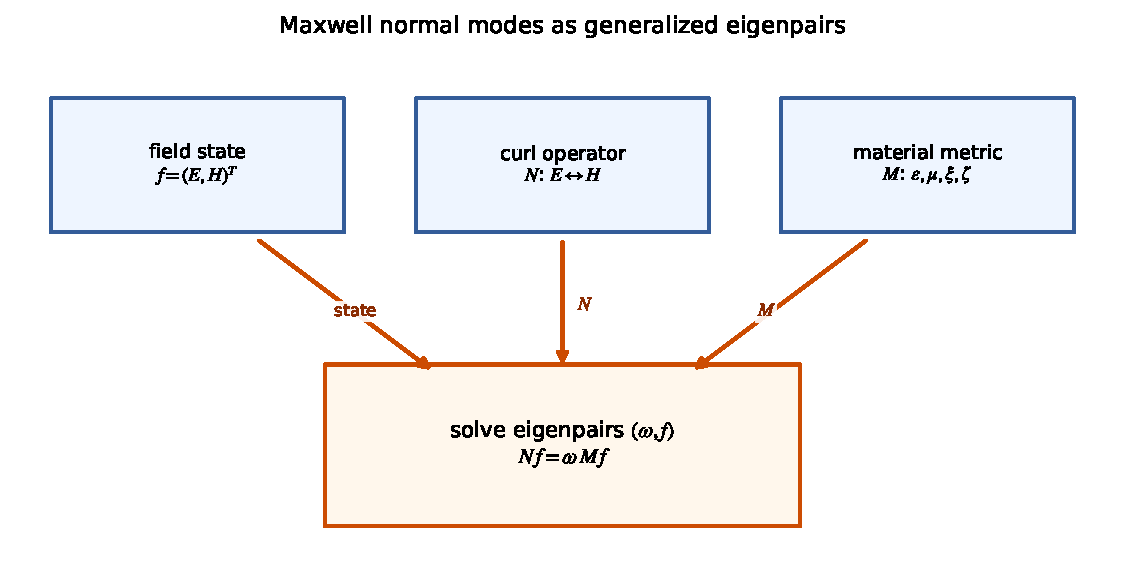
\includegraphics[width=0.88\textwidth]{figures/fig_ch02_maxwell_blocks.pdf}
  \caption{Maxwell's equations as a six-component normal-mode problem.
  The electromagnetic field state $\mathbf{f}=(\mathbf{E},\mathbf{H})^T$
  is acted on by the curl operator $N$, while the material tensor $M$
  supplies the energy metric.  Topological band theory for photons starts
  only after this metric structure is fixed.}
  \label{fig:ch02-maxwell-blocks}
\end{figure}

\section*{Exercises}

\begin{exercise}
  Verify by direct computation that the $6\times6$ momentum-space curl
  operator $\Maxop(\kvec)$ defined in \eqref{eq:ch2-maxop-k} is
  Hermitian.  \emph{Hint:} write out the full matrix for a general
  $\kvec=(k_x,k_y,k_z)$ and check that it equals its conjugate
  transpose.
\end{exercise}

\begin{exercise}
  For an isotropic medium with scalar $\varepsilon$ and $\mu$, show
  that the eigenvalues of the $6\times 6$ matrix
  $\Mmat^{-1}\Maxop(\kvec)$ are
  $\omega=\pm|\kvec|/\sqrt{\varepsilon_0\mu_0\varepsilon\mu}$
  (each twofold degenerate, corresponding to two transverse
  polarisations) and $\omega=0$ (twofold, corresponding to
  longitudinal modes).  Identify the physical content of each.
\end{exercise}

\begin{exercise}
  The gyrotropic permeability tensor \eqref{eq:ch2-gyrotropic-mu} has
  eigenvalues $\mu_\perp\pm\kappa$ for circular polarisations and
  $\mu_z$ for the $z$-component.  Derive the two circular-polarisation
  refractive indices $n_\pm=\sqrt{\varepsilon(\mu_\perp\pm\kappa)}$
  for a plane wave propagating along $\hat{z}$ in a medium with scalar
  permittivity $\varepsilon$ and gyrotropic permeability.  Show that
  the Faraday rotation per unit length is
  $\theta_F=\omega(n_+-n_-)/(2c)$.
\end{exercise}

\begin{exercise}
  Prove that the complex Poynting identity
  \eqref{eq:ch2-complex-poynting} holds by starting from the curl
  equations \eqref{eq:ch2-maxwell-freq} and using the vector identity
  $\nabla\cdot(\mathbf{A}\times\mathbf{B})
  =\mathbf{B}\cdot(\nabla\times\mathbf{A})
  -\mathbf{A}\cdot(\nabla\times\mathbf{B})$.
\end{exercise}

\begin{exercise}
  Show that for a lossless nondispersive medium, the divergence of the
  time-averaged Poynting vector vanishes:
  $\nabla\cdot\langle\Sfield\rangle=0$.  What additional condition is
  needed for this to hold in a dispersive medium?
\end{exercise}

\begin{exercise}
  Starting from the bianisotropic constitutive relation
  \eqref{eq:ch2-bianisotropic}, verify explicitly that the
  time-reversal condition \eqref{eq:ch2-TR-condition} applied to
  $\Mmat$ yields the block conditions \eqref{eq:ch2-TR-blocks}.
\end{exercise}


\chapter{Normal Modes and the Electromagnetic Inner Product}
\label{ch:normal-modes}
% ======================================================================
%  Chapter 3 — Normal Modes and the Electromagnetic Inner Product
% ======================================================================

\section{Why the inner product matters}
\label{sec:ch3-why-ip}

In quantum mechanics, the Hilbert-space inner product
$\langle\psi|\phi\rangle=\int\psi^*\phi\,\dd^3r$ is so natural that it
is rarely questioned.  The Hamiltonian is self-adjoint under this inner
product, eigenvalues are real, and eigenstates are orthogonal---all
with the standard $L^2$ norm.

The Maxwell eigenvalue equation
\begin{equation}\label{eq:ch3-evp-recap}
  \Maxop\,\emfield = \omega\,\Mmat\,\emfield
\end{equation}
from \chref{ch:maxwell-dynamics} is \emph{not} a standard eigenvalue
problem.  The material matrix $\Mmat$ appears on the right-hand side,
making this a \emph{generalised} eigenproblem.  If we naively define an
``effective Hamiltonian'' $\Hamop=\Mmat^{-1}\Maxop$ and write
$\Hamop\emfield=\omega\emfield$, the operator $\Hamop$ is generally
\emph{not} Hermitian under the standard inner product
$\emfield_1^\dagger\emfield_2$.

This means that the standard $L^2$ inner product is the \emph{wrong}
inner product for electromagnetic normal modes.  Using it leads to
non-orthogonal modes, non-gauge-invariant Berry connections, and
incorrect topological invariants.  The correct inner product is the
\emph{electromagnetic energy inner product}, weighted by the material
matrix $\Mmat$ (or, in dispersive media, by the energy metric
$\Mgmat$) \cite{nittis2020equivalence}.  Establishing this inner product rigorously is the central
task of this chapter.

\section{Self-adjointness of the Maxwell operator}
\label{sec:ch3-self-adjoint}

\subsection{The nondispersive case}
\label{sec:ch3-self-adjoint-nondisp}

Consider first a nondispersive lossless medium, so that $\Mmat(\rvec)$
is Hermitian and frequency-independent.  Define the electromagnetic
inner product over a domain $V$ (which will later be specialised to a
unit cell):
\begin{equation}\label{eq:ch3-em-ip}
  \boxed{%
  \emip{\emfield_1}{\emfield_2}
  \;\equiv\;
  \int_V \emfield_1^\dagger(\rvec)\cdot\Mmat(\rvec)
         \cdot\emfield_2(\rvec)\,\dd^3r\,.}
\end{equation}
Since $\Mmat=\Mmat^\dagger$, this is a sesquilinear form; since $\Mmat$
is positive definite (\secref{sec:ch2-dispersive-energy}), it is
positive definite and hence a genuine inner product.

\begin{theorem}[Self-adjointness of the Maxwell operator]
  \label{thm:ch3-self-adjoint}
  Let $\Mmat(\rvec)$ be Hermitian and positive definite, and let
  $\emfield_1$, $\emfield_2$ be smooth six-component fields satisfying
  appropriate boundary conditions (periodic, or vanishing at infinity).
  Then the Maxwell curl operator $\Maxop$ is self-adjoint with respect
  to the electromagnetic inner product:
  \begin{equation}\label{eq:ch3-self-adj-statement}
    \emip{\emfield_1}{\Mmat^{-1}\Maxop\,\emfield_2}
    = \emip{\Mmat^{-1}\Maxop\,\emfield_1}{\emfield_2}\,.
  \end{equation}
  Equivalently, writing $\Hamop=\Mmat^{-1}\Maxop$:
  \begin{equation}\label{eq:ch3-H-self-adj}
    \emip{\emfield_1}{\Hamop\,\emfield_2}
    = \emip{\Hamop\,\emfield_1}{\emfield_2}\,.
  \end{equation}
\end{theorem}

\begin{proof}
We need to show that
\begin{equation}\label{eq:ch3-proof-target}
  \int_V \emfield_1^\dagger\,\Mmat\,(\Mmat^{-1}\Maxop\,\emfield_2)\,\dd^3r
  = \int_V (\Mmat^{-1}\Maxop\,\emfield_1)^\dagger\,\Mmat\,\emfield_2\,\dd^3r\,.
\end{equation}
The left-hand side simplifies to $\int_V\emfield_1^\dagger\,\Maxop\,\emfield_2\,\dd^3r$.
The right-hand side simplifies to
$\int_V(\Maxop\,\emfield_1)^\dagger\,\Mmat^{-\dagger}\Mmat\,\emfield_2\,\dd^3r
=\int_V(\Maxop\,\emfield_1)^\dagger\,\emfield_2\,\dd^3r$
since $\Mmat^{-\dagger}\Mmat=\mathbf{I}$ for Hermitian $\Mmat$.
So we need to prove
\begin{equation}\label{eq:ch3-maxop-sa}
  \int_V \emfield_1^\dagger\,\Maxop\,\emfield_2\,\dd^3r
  = \int_V (\Maxop\,\emfield_1)^\dagger\,\emfield_2\,\dd^3r\,,
\end{equation}
i.e., $\Maxop$ itself is self-adjoint under the \emph{standard} $L^2$
inner product.

Write $\emfield_i=(\Efield_i,\Hfield_i)^T$.  Then
\begin{equation}
  \emfield_1^\dagger\,\Maxop\,\emfield_2
  = \Efield_1^*\cdot(\ii\nabla\times\Hfield_2)
    + \Hfield_1^*\cdot(-\ii\nabla\times\Efield_2)\,.
\end{equation}
Similarly,
\begin{equation}
  (\Maxop\,\emfield_1)^\dagger\,\emfield_2
  = (-\ii\nabla\times\Hfield_1)^*\cdot\Efield_2
    + (\ii\nabla\times\Efield_1)^*\cdot\Hfield_2
  = \ii(\nabla\times\Hfield_1^*)\cdot\Efield_2
    - \ii(\nabla\times\Efield_1^*)\cdot\Hfield_2\,.
\end{equation}
Taking the difference:
\begin{align}
  &\emfield_1^\dagger\,\Maxop\,\emfield_2
   - (\Maxop\,\emfield_1)^\dagger\,\emfield_2 \notag\\
  &= \ii\bigl[
    \Efield_1^*\cdot(\nabla\times\Hfield_2)
    - (\nabla\times\Hfield_1^*)\cdot\Efield_2
  \bigr]
  -\ii\bigl[
    \Hfield_1^*\cdot(\nabla\times\Efield_2)
    - (\nabla\times\Efield_1^*)\cdot\Hfield_2
  \bigr]. \label{eq:ch3-sa-diff}
\end{align}
Each bracket is a total divergence.  Using the identity
$\mathbf{A}\cdot(\nabla\times\mathbf{B})
-(\nabla\times\mathbf{A})\cdot\mathbf{B}
= -\nabla\cdot(\mathbf{A}\times\mathbf{B})$:
\begin{equation}\label{eq:ch3-sa-divergence}
  \emfield_1^\dagger\,\Maxop\,\emfield_2
  - (\Maxop\,\emfield_1)^\dagger\,\emfield_2
  = -\ii\,\nabla\cdot\bigl(
    \Efield_1^*\times\Hfield_2
    - \Hfield_1^*\times\Efield_2
  \bigr).
\end{equation}
Integrating over $V$ and applying the divergence theorem:
\begin{equation}\label{eq:ch3-boundary-term}
  \int_V\bigl(\emfield_1^\dagger\,\Maxop\,\emfield_2
  - (\Maxop\,\emfield_1)^\dagger\,\emfield_2\bigr)\dd^3r
  = -\ii\oint_{\partial V}\bigl(
    \Efield_1^*\times\Hfield_2
    - \Hfield_1^*\times\Efield_2
  \bigr)\cdot\hat{n}\,\dd A\,.
\end{equation}
The surface integral vanishes when:
\begin{enumerate}[label=(\alph*)]
  \item the fields satisfy \emph{periodic boundary conditions}
    ($\emfield(\rvec+\avec)=\ee^{\ii\kvec\cdot\avec}\emfield(\rvec)$
    for lattice vector $\avec$), since opposite faces of the unit cell
    contribute equal and opposite terms; or
  \item the fields decay sufficiently fast at infinity; or
  \item the domain has perfectly conducting or perfectly magnetic boundaries.
\end{enumerate}
Under any of these conditions,
$\int_V\emfield_1^\dagger\Maxop\emfield_2\,\dd^3r
=\int_V(\Maxop\emfield_1)^\dagger\emfield_2\,\dd^3r$,
establishing \eqref{eq:ch3-maxop-sa} and hence
\eqref{eq:ch3-H-self-adj}.
\end{proof}

\begin{corollary}[Real eigenfrequencies]
  \label{cor:ch3-real-omega}
  Every eigenfrequency $\omega_n$ of the Maxwell normal-mode problem
  $\Hamop\emfield_n=\omega_n\emfield_n$ is real.
\end{corollary}

\begin{proof}
From self-adjointness:
$\omega_n\emip{\emfield_n}{\emfield_n}
=\emip{\emfield_n}{\Hamop\emfield_n}
=\emip{\Hamop\emfield_n}{\emfield_n}
=\omega_n^*\emip{\emfield_n}{\emfield_n}$.
Since $\emip{\emfield_n}{\emfield_n}>0$, we conclude $\omega_n=\omega_n^*$.
\end{proof}

\subsection{Orthogonality of modes}
\label{sec:ch3-orthogonality} \cite{press2026photonic}

\begin{proposition}[Mode orthogonality]
  \label{prop:ch3-orthogonality}
  Eigenmodes at different eigenfrequencies are orthogonal under the
  electromagnetic inner product:
  \begin{equation}\label{eq:ch3-orthogonality}
    \omega_n\neq\omega_m
    \quad\Longrightarrow\quad
    \emip{\emfield_n}{\emfield_m}=0\,.
  \end{equation}
\end{proposition}

\begin{proof}
Self-adjointness gives
$\emip{\emfield_n}{\Hamop\emfield_m}
=\emip{\Hamop\emfield_n}{\emfield_m}$, i.e.,
$\omega_m\emip{\emfield_n}{\emfield_m}
=\omega_n^*\emip{\emfield_n}{\emfield_m}
=\omega_n\emip{\emfield_n}{\emfield_m}$
(using $\omega_n\in\mathbb{R}$).  Hence
$(\omega_m-\omega_n)\emip{\emfield_n}{\emfield_m}=0$; if
$\omega_n\neq\omega_m$, the inner product vanishes.
\end{proof}

We adopt the \emph{energy normalisation convention}:
\begin{equation}\label{eq:ch3-normalisation}
  \emip{\emfield_n}{\emfield_m}
  = \int_V\emfield_n^\dagger\,\Mmat\,\emfield_m\,\dd^3r
  = \delta_{nm}\,.
\end{equation}
The physical meaning of $\emip{\emfield_n}{\emfield_n}=1$ is that the
mode carries unit time-averaged electromagnetic energy per unit cell (in
a periodic medium) or per normalisation volume.

\section{The energy-weighted field}
\label{sec:ch3-energy-weighted}

The electromagnetic inner product \eqref{eq:ch3-em-ip} is perfectly
rigorous \cite{gangaraj2016berry,raghu2008analogs}, but it is sometimes convenient to work with a
\emph{standard}-Hermitian formulation.  This is achieved by a change of
variables that absorbs $\Mmat$ into the field.

Since $\Mmat$ is Hermitian and positive definite, it has a unique
positive-definite Hermitian square root $\Mmat^{1/2}$.  Define the
\emph{energy-weighted field}
\begin{equation}\label{eq:ch3-w-def}
  \boxed{%
  \emfieldw(\rvec) \equiv \Mmat^{1/2}(\rvec)\,\emfield(\rvec)\,.}
\end{equation}
Then the electromagnetic inner product becomes the standard $L^2$ inner
product for $\emfieldw$:
\begin{equation}\label{eq:ch3-w-ip}
  \emip{\emfield_1}{\emfield_2}
  = \int_V\emfield_1^\dagger\Mmat\emfield_2\,\dd^3r
  = \int_V\emfieldw_1^\dagger\,\emfieldw_2\,\dd^3r\,.
\end{equation}
The eigenvalue equation in terms of $\emfieldw$ becomes
\begin{equation}\label{eq:ch3-w-evp}
  \tilde{\Hamop}(\rvec)\,\emfieldw(\rvec)
  = \omega\,\emfieldw(\rvec)\,,
  \qquad
  \tilde{\Hamop}
  = \Mmat^{-1/2}\,\Maxop\,\Mmat^{-1/2}\,,
\end{equation}
and $\tilde{\Hamop}$ is Hermitian under the standard inner product.

\begin{remark}
The energy-weighted formulation is useful for formal proofs and for
connecting to the quantum-mechanical literature, where Berry connections
are always defined with respect to the standard inner product.  However,
the original formulation in terms of $\emfield$ and $\Mmat$ is often
more convenient in practice, because $\emfield=(\Efield,\Hfield)^T$
has direct physical meaning, while $\emfieldw=\Mmat^{1/2}\emfield$ does
not correspond to any simply measurable field.  We will use both
formulations interchangeably and state which inner product is being used
at each stage.
\end{remark}

\section{Extension to dispersive media}
\label{sec:ch3-dispersive}

\subsection{The generalised eigenvalue problem}
\label{sec:ch3-gen-evp}

Real magneto-optical materials are always dispersive: the gyrotropic
parameter $\kappa$ in \eqref{eq:ch2-gyrotropic-mu} depends on
frequency, as do $\varepsilon$, $\mu_\perp$, and all other material
parameters
\cite{wang2007reflection}.  The material matrix is then $\Mmat=\Mmat(\rvec,\omega)$,
and the Maxwell eigenvalue equation
\begin{equation}\label{eq:ch3-gen-evp}
  \Maxop\,\emfield = \omega\,\Mmat(\omega)\,\emfield
\end{equation}
is a \emph{nonlinear} eigenvalue problem in $\omega$: the eigenvalue
appears both explicitly and inside $\Mmat$.  This is qualitatively
different from the Schr\"odinger equation, where the Hamiltonian does
not depend on the energy eigenvalue.

Following Haldane and Raghu, we treat this as a generalised eigenvalue
problem.  For a Bloch mode in a periodic medium, the cell-periodic
eigenproblem takes the form
\begin{equation}\label{eq:ch3-bloch-gen-evp}
  \Maxop(\kvec)\,\mathbf{u}_{n\kvec}(\rvec)
  = \omega_{n\kvec}\,\Mmat(\rvec,\omega_{n\kvec})\,
    \mathbf{u}_{n\kvec}(\rvec)\,,
\end{equation}
where $\Maxop(\kvec)$ is the curl operator with $\nabla$ replaced by
$\nabla+\ii\kvec$ (incorporating the Bloch phase).

\subsection{The energy metric as inner product}
\label{sec:ch3-energy-metric-ip}

The self-adjointness proof of \secref{sec:ch3-self-adjoint-nondisp}
relied on $\Mmat$ being the same for both modes.  In the dispersive
case, two modes $\emfield_n$ and $\emfield_m$ at \emph{different}
frequencies see \emph{different} material matrices
$\Mmat(\omega_n)\neq\Mmat(\omega_m)$, and the standard orthogonality
argument breaks down.

The resolution was provided by the energy metric
$\Mgmat(\omega)=\partial_\omega[\omega\Mmat(\omega)]$ introduced in
\eqref{eq:ch2-energy-metric}.  The key result is:

\begin{theorem}[Orthogonality in dispersive media]
  \label{thm:ch3-dispersive-orth}
  Let $\Mmat(\rvec,\omega)$ be Hermitian for real $\omega$, and let
  $\Mgmat(\rvec,\omega)=\partial_\omega[\omega\Mmat(\rvec,\omega)]$ be
  positive definite at all physical eigenfrequencies.  Then two Bloch
  eigenmodes $\mathbf{u}_{n\kvec}$ and $\mathbf{u}_{m\kvec}$ at the
  same wavevector $\kvec$ but different frequencies satisfy the
  \emph{exact} relation
  \begin{equation}\label{eq:ch3-dispersive-orth}
    \omega_n\int_{\mathrm{cell}}
    \mathbf{u}_{n\kvec}^\dagger\,\Mmat(\omega_n)
    \,\mathbf{u}_{m\kvec}\,\dd^3r
    = \omega_m\int_{\mathrm{cell}}
    \mathbf{u}_{n\kvec}^\dagger\,\Mmat(\omega_m)
    \,\mathbf{u}_{m\kvec}\,\dd^3r\,.
  \end{equation}
  When the two frequencies are close ($\omega_m\to\omega_n$), this
  reduces to $\int\mathbf{u}_n^\dagger\Mgmat(\omega_n)\mathbf{u}_m
  \,\dd^3r=0$.  The group-velocity metric $\Mgmat$ therefore plays
  the role of the orthogonality metric for near-degenerate modes and
  also determines the self-overlap normalization
  $\int\mathbf{u}_n^\dagger\Mgmat(\omega_n)\mathbf{u}_n\,\dd^3r>0$.
\end{theorem}

\begin{figure}[!t]
  \centering
  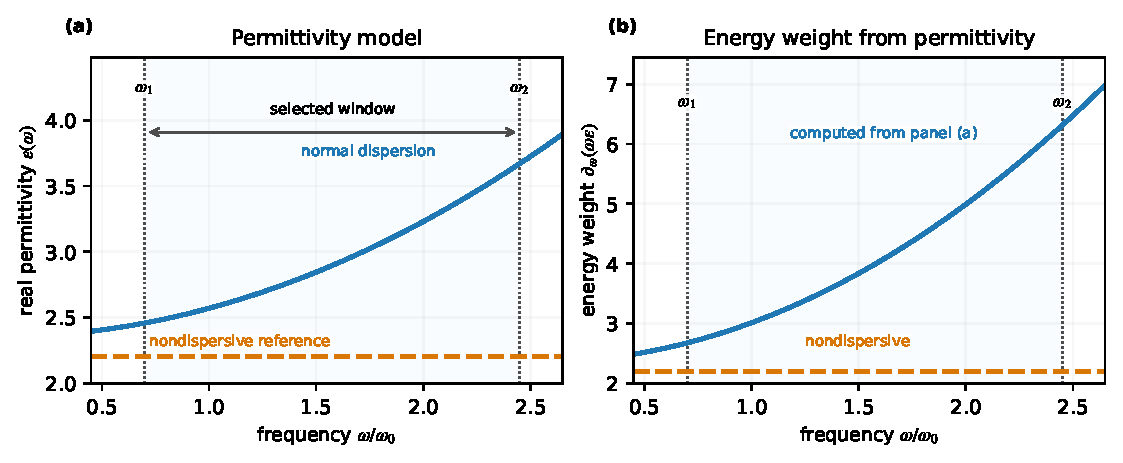
\includegraphics[width=0.92\textwidth]{figures/fig_ch03_dispersive_metric_step199.pdf}
  \caption{Dispersive energy metric and its frequency dependence.
  \textbf{(a)}~Representative dielectric function $\varepsilon(\omega)$
  of a Lorentzian medium, showing a selected lossless window between
  frequencies $\omega_1$ and $\omega_2$ where $\varepsilon$ is real and
  positive.  The dashed line marks the nondispersive reference level.
  \textbf{(b)}~The corresponding energy-metric weight
  $\partial_\omega[\omega\varepsilon(\omega)]$ computed from panel~(a).
  In the lossless window the weight exceeds unity and increases with
  frequency, reflecting the additional electromagnetic energy stored in
  the dispersive polarisation of the medium.  The orthogonality of
  Bloch modes in dispersive media
  (Theorem~\ref{thm:ch3-dispersive-orth}) is governed by this
  frequency-dependent metric rather than by $\varepsilon(\omega)$
  alone.}
  \label{fig:ch03-dispersive-metric}
\end{figure}


\begin{proof}
Start from the eigenvalue equations for modes $n$ and $m$:
\begin{align}
  \Maxop(\kvec)\,\mathbf{u}_n &= \omega_n\,\Mmat(\omega_n)\,\mathbf{u}_n\,,
  \label{eq:ch3-disp-evp-n}\\
  \Maxop(\kvec)\,\mathbf{u}_m &= \omega_m\,\Mmat(\omega_m)\,\mathbf{u}_m\,.
  \label{eq:ch3-disp-evp-m}
\end{align}
Take the inner product of \eqref{eq:ch3-disp-evp-m} with
$\mathbf{u}_n$ (standard $L^2$, with periodic boundary conditions as
before):
\begin{equation}
  \int\mathbf{u}_n^\dagger\,\Maxop(\kvec)\,\mathbf{u}_m\,\dd^3r
  = \omega_m\int\mathbf{u}_n^\dagger\,\Mmat(\omega_m)\,\mathbf{u}_m\,\dd^3r\,.
\end{equation}
By the self-adjointness of $\Maxop(\kvec)$ (the boundary term vanishes
for Bloch-periodic fields), the left-hand side also equals
$\int(\Maxop(\kvec)\mathbf{u}_n)^\dagger\mathbf{u}_m\,\dd^3r
=\omega_n^*\int\mathbf{u}_n^\dagger\Mmat^\dagger(\omega_n)\mathbf{u}_m\,\dd^3r
=\omega_n\int\mathbf{u}_n^\dagger\Mmat(\omega_n)\mathbf{u}_m\,\dd^3r$.
(We used $\omega_n\in\mathbb{R}$ and $\Mmat^\dagger=\Mmat$.)

Therefore:
\begin{equation}\label{eq:ch3-disp-orth-step}
  \omega_n\int\mathbf{u}_n^\dagger\Mmat(\omega_n)\mathbf{u}_m\,\dd^3r
  = \omega_m\int\mathbf{u}_n^\dagger\Mmat(\omega_m)\mathbf{u}_m\,\dd^3r\,.
\end{equation}
Equation~\eqref{eq:ch3-disp-orth-step} is already the desired exact
off-diagonal relation.  Equivalently,
\begin{equation}\label{eq:ch3-divided-difference-orth}
  \int \mathbf{u}_n^\dagger
  \left[
    \omega_n\Mmat(\omega_n)-\omega_m\Mmat(\omega_m)
  \right]
  \mathbf{u}_m\,\dd^3r = 0\,.
\end{equation}
For $n\neq m$ this may be viewed as orthogonality with respect to the
frequency divided-difference operator
\begin{equation}\label{eq:ch3-divided-difference-metric}
  \Mmat_{nm}^{\mathrm{dd}}
  = \frac{\omega_n\Mmat(\omega_n)-\omega_m\Mmat(\omega_m)}
  {\omega_n-\omega_m}\,.
\end{equation}
In the limit $\omega_m\to\omega_n$, this operator tends
$\partial_\omega[\omega\Mmat(\omega)]_{\omega_n}=\Mgmat(\omega_n)$.
Thus $\Mgmat$ is the correct self-overlap and near-degenerate metric,
while the exact off-diagonal relation for separated frequencies is the
divided-difference relation above.
\end{proof}

\begin{remark}
The proof shows that the energy metric $\Mgmat$ arises naturally as the
``linearisation'' of the nonlinear eigenvalue problem around a given
eigenfrequency.  The positive definiteness of $\Mgmat$ is not just a
convenient assumption; it is the physical stability condition ensuring
that each mode carries positive energy and that the eigenfrequencies
are locally non-degenerate as a function of $\omega$.
\end{remark}

\subsection{Normalisation in dispersive media}
\label{sec:ch3-disp-norm}

The natural normalisation convention for dispersive media is
\begin{equation}\label{eq:ch3-disp-norm}
  \boxed{%
  \eip{\mathbf{u}_n}{\mathbf{u}_m}
  \;\equiv\;
  \int_{\mathrm{cell}}
  \mathbf{u}_{n\kvec}^\dagger(\rvec)\,
  \Mgmat(\rvec,\omega_{n\kvec})\,
  \mathbf{u}_{m\kvec}(\rvec)\,\dd^3r
  = \delta_{nm}\,.}
\end{equation}
With this normalisation, the time-averaged electromagnetic energy stored
in the mode equals unity per unit cell, including the energy stored in
the material degrees of freedom (dispersive polarisation).

In the nondispersive limit $\partial\Mmat/\partial\omega=0$, the energy
metric reduces to $\Mgmat=\Mmat$ and
\eqref{eq:ch3-disp-norm} becomes \eqref{eq:ch3-normalisation}.

\subsection{Energy-weighted fields in dispersive media}
\label{sec:ch3-disp-weighted}

Since $\Mgmat(\omega)$ is Hermitian and positive definite at physical
eigenfrequencies, it also has a unique positive-definite square root.
Define
\begin{equation}\label{eq:ch3-disp-w}
  \emfieldw_{n\kvec}(\rvec)
  = \Mgmat^{1/2}(\rvec,\omega_{n\kvec})\,\mathbf{u}_{n\kvec}(\rvec)\,.
\end{equation}
Then $\int\emfieldw_n^\dagger\emfieldw_m\,\dd^3r=\delta_{nm}$, and all
Berry-geometry formulas can be written in terms of $\emfieldw$ with the
standard inner product.

\begin{remark}
There is a subtlety: $\Mgmat$ depends on $\omega_n(\kvec)$, which
varies with $\kvec$.  When computing Berry connections (derivatives
with respect to $\kvec$), one must account for this implicit $\kvec$
dependence through $\omega_n(\kvec)$.  We will address this carefully in
\chref{ch:geometry-bands}.
\end{remark}

\section{The role of the divergence constraint}
\label{sec:ch3-divergence}

The Maxwell curl equations \eqref{eq:ch3-evp-recap} are supplemented by
the divergence constraints $\nabla\cdot\Dfield=0$ and
$\nabla\cdot\Bfield=0$.  In the six-component formalism, these become
\begin{equation}\label{eq:ch3-div-constraint}
  \nabla\cdot\bigl(\Mmat\,\emfield\bigr) = 0\,,
\end{equation}
which in momentum space reads $(\kvec+\Gvec)\cdot(\Mmat\,\hat{\mathbf{u}}_\Gvec)=0$
for each Fourier component.

\paragraph{Transverse and longitudinal modes.}
For an isotropic medium with scalar $\varepsilon$ and $\mu$, the
eigenmodes of the Maxwell operator split into two classes:
\begin{itemize}
  \item \emph{Transverse modes} with $\kvec\cdot\Efield=0$ and
    $\kvec\cdot\Hfield=0$.  These have nonzero eigenfrequencies
    $\omega\neq0$ and represent propagating electromagnetic waves.
  \item \emph{Longitudinal modes} with $\nabla\times\Efield=0$ and
    $\nabla\times\Hfield=0$, satisfying
    $\Maxop\,\emfield_L=0$.  These are the null space of $\Maxop$
    and have $\omega=0$.
\end{itemize}
The divergence constraint eliminates the longitudinal modes from the
physical spectrum.  In a photonic crystal, the situation is analogous:
the physical modes lie in the transverse subspace satisfying
\eqref{eq:ch3-div-constraint}.

\begin{remark}
The longitudinal modes are often silently excluded in the photonic
band-structure literature by working directly with the second-order
equation $\nabla\times(\mu^{-1}\nabla\times\Efield)
=(\omega^2/c^2)\varepsilon\Efield$, which is automatically transverse
when applied to divergence-free fields.  The first-order six-component
formulation keeps them visible, which is important for rigour:
one must verify that the Berry curvature and Chern numbers are computed
only over the physical (transverse) bands.
\end{remark}

\section{Completeness and spectral theory}
\label{sec:ch3-completeness} \cite{initio2026pdf}

\subsection{Mode expansion}
\label{sec:ch3-expansion}

In a lossless nondispersive medium occupying a finite domain $V$ with
appropriate boundary conditions, the transverse eigenmodes
$\{\emfield_n\}$ of $\Hamop=\Mmat^{-1}\Maxop$ form a complete
orthonormal set with respect to the electromagnetic inner product.  Any
transverse six-component field can be expanded as
\begin{equation}\label{eq:ch3-mode-expansion}
  \emfield(\rvec) = \sum_n c_n\,\emfield_n(\rvec)\,,
  \qquad
  c_n = \emip{\emfield_n}{\emfield}\,.
\end{equation}
This is the electromagnetic analog of the expansion of a quantum state
in energy eigenstates.

For a periodic medium, completeness applies within each Bloch sector
at fixed $\kvec$: the cell-periodic modes
$\{\mathbf{u}_{n\kvec}\}_{n=1}^{\infty}$ span the transverse subspace
of $L^2$-periodic functions on the unit cell.

\subsection{Spectral properties}
\label{sec:ch3-spectral}

The eigenfrequencies $\omega_n(\kvec)$ are real and can be ordered:
\begin{equation}
  0 < \omega_1(\kvec) \leq \omega_2(\kvec) \leq \cdots\,.
\end{equation}
(We exclude the $\omega=0$ longitudinal modes.)  As $\kvec$ varies
over the Brillouin zone, each $\omega_n(\kvec)$ traces out a
\emph{band}.  The bands may overlap (when $\omega_n(\kvec)$ and
$\omega_{n+1}(\kvec')$ have the same value for different $\kvec,\kvec'$)
or may be separated by \emph{band gaps}: frequency intervals in which
no eigenfrequency exists for any $\kvec$.

The existence and width of band gaps depend on the contrast of the
material parameters and the geometry of the periodic structure.  We will
study the band structure in detail in \chref{ch:periodic-media}.

\section{Summary of key formulas}
\label{sec:ch3-summary}

For reference, we collect the central results of this chapter.

\begin{enumerate}
  \item \textbf{Electromagnetic inner product (nondispersive):}
  \begin{equation}
    \emip{\emfield_1}{\emfield_2}
    = \int_V\emfield_1^\dagger\,\Mmat\,\emfield_2\,\dd^3r\,.
    \tag{\ref{eq:ch3-em-ip}}
  \end{equation}

  \item \textbf{Self-adjointness:}
  $\Hamop=\Mmat^{-1}\Maxop$ is self-adjoint under $\langle\cdot,\cdot\rangle_\Mmat$.

  \item \textbf{Real eigenfrequencies, orthogonal modes:}
  $\omega_n\in\mathbb{R}$;\quad
  $\emip{\emfield_n}{\emfield_m}=\delta_{nm}$.

  \item \textbf{Energy-weighted field:}
  $\emfieldw=\Mmat^{1/2}\emfield$;\quad
  standard Hermitian eigenvalue problem for $\emfieldw$.

  \item \textbf{Dispersive energy metric:} \cite{gangaraj2016berry,silveirinha2016bulk}
  \begin{equation}
    \Mgmat(\omega)=\pderiv{}{\omega}[\omega\Mmat(\omega)]\,.
    \tag{\ref{eq:ch2-energy-metric}}
  \end{equation}

  \item \textbf{Orthogonality in dispersive media:}
  \begin{equation}
    \eip{\mathbf{u}_n}{\mathbf{u}_m}
    = \int_{\mathrm{cell}}
    \mathbf{u}_n^\dagger\,\Mgmat(\omega_n)\,\mathbf{u}_m\,\dd^3r
    = \delta_{nm}\,.
    \tag{\ref{eq:ch3-disp-norm}}
  \end{equation}
\end{enumerate}

These results are the foundation on which all Berry-geometric and
topological statements in the rest of the book are built.  The Berry
connection, Berry curvature, and Chern number for electromagnetic bands
must always be defined using the material-weighted inner product
$\langle\cdot,\cdot\rangle_\Mmat$ or its dispersive generalisation
$\langle\cdot,\cdot\rangle_{\Mgmat}$.  Using the wrong inner product---a
mistake easily made when importing formulas from quantum
mechanics---invalidates the topological invariants.

\section{The dispersive energy metric: derivation and meaning}
\label{sec:ch3-dispersive-derivation}

When the material parameters depend on frequency---as they must for
any causal material---the non-dispersive energy density
$\mathcal{U}=\frac{1}{2}\emfield^\dagger\Mmat(\omega)\emfield$ is
not the physically correct energy stored in the field.  The correct
expression is the Brillouin energy density, derived as follows.

\subsection{Derivation from energy conservation}
\label{sec:ch3-brillouin-derivation}

Consider a monochromatic field at frequency $\omega$ with a slowly
varying envelope.  The time-averaged energy density stored in the
medium is \cite{gangaraj2016berry}
\begin{equation}\label{eq:ch3-brillouin-energy}
  \langle\mathcal{U}\rangle
  = \frac{1}{4}\emfield^\dagger
  \frac{\partial[\omega\Mmat(\omega)]}{\partial\omega}\,\emfield
  = \frac{1}{4}\emfield^\dagger\Mgmat(\omega)\,\emfield\,.
\end{equation}
The dispersive energy metric $\Mgmat(\omega)
=\partial_\omega[\omega\Mmat(\omega)]$ appears because the energy
stored in the oscillators of the medium must be included alongside
the free-field energy.

For a non-dispersive material,
$\Mgmat=\Mmat+\omega\partial_\omega\Mmat=\Mmat$ (since
$\partial_\omega\Mmat=0$), and the Brillouin energy reduces to
the familiar non-dispersive form.

\subsection{Positivity from passivity}
\label{sec:ch3-positivity}

For a passive material (no gain), the Kramers--Kronig relations
guarantee that $\Mgmat(\omega)$ is positive definite at every
real frequency outside the absorption bands.  The physical argument
is simple: a passive material can only store (not create) energy,
so $\langle\mathcal{U}\rangle$ must be positive for all nonzero
field amplitudes \cite{silveirinha2016bulk}.

This positivity is essential for the entire topological framework of
this book: the electromagnetic inner product
$\eip{\emfield_1}{\emfield_2}
=\int\emfield_1^\dagger\Mgmat\,\emfield_2\,\dd^3 r$ is positive
definite, making the eigenproblem Hermitian and the Berry connection
well defined.  If $\Mgmat$ lost positive definiteness (as can happen
near a gain-induced instability), the Hermitian structure would break
and the Chern number would need to be redefined through the
non-Hermitian methods of Chapter~\ref{ch:non-hermitian}.

\subsection{The dispersive inner product and Berry connection}
\label{sec:ch3-dispersive-berry}

The dispersive energy metric enters the Berry connection through the
replacement $\Mmat\to\Mgmat$ everywhere the inner product appears.
Specifically, the Berry connection for band $n$ is
\begin{equation}\label{eq:ch3-dispersive-berry}
  \mathcal{A}_{n,a}(\kvec)
  = \ii\int_{\mathrm{cell}}
  \mathbf{u}_{n\kvec}^\dagger\,\Mgmat(\omega_{n\kvec})\,
  \partial_{k_a}\mathbf{u}_{n\kvec}\,\dd^3 r\,,
\end{equation}
where $\Mgmat(\omega_{n\kvec})$ is evaluated at the band frequency.
This formula reduces to the non-dispersive Berry connection when
$\Mgmat=\Mmat$, but it is the dispersive form that must be used for
real photonic crystals with frequency-dependent material response
\cite{gangaraj2016berry,ozawa2018topological}.

\section{Orthogonality subtleties}
\label{sec:ch3-orthogonality-subtleties}

\subsection{Degenerate modes and gauge freedom}
\label{sec:ch3-degenerate-gauge}

When two or more bands are degenerate at a point $\kvec_0$, the
individual modes $\mathbf{u}_{n\kvec_0}$ are not uniquely determined:
any unitary rotation within the degenerate subspace produces an
equally valid set of eigenmodes.  This gauge freedom means that the
Abelian Berry connection $\mathcal{A}_n$ is not well defined at
$\kvec_0$; instead, one must use the non-Abelian Berry connection
$\mathcal{A}_{mn}=\ii\eip{\mathbf{u}_m}{\nabla_\kvec\mathbf{u}_n}$,
where $m$ and $n$ range over the degenerate bands.

The non-Abelian connection transforms as a gauge field under unitary
rotations of the degenerate subspace, and its curvature
$\mathcal{F}_{mn}=\partial_a\mathcal{A}_{mn,b}
-\partial_b\mathcal{A}_{mn,a}
+\ii[\mathcal{A}_a,\mathcal{A}_b]_{mn}$
is gauge-covariant.  The Chern number of a degenerate band group is
$\Chern=\frac{1}{2\pi}\int_{\mathrm{BZ}}\Tr\,\mathcal{F}\,\dd^2 k$,
which is gauge-invariant and well defined even at the degeneracy
points \cite{gangaraj2016berry,ozawa2018topological}.

\subsection{Spurious modes and the null space}
\label{sec:ch3-spurious}

The Maxwell eigenproblem \eqref{eq:ch2-maxwell-matrix} admits spurious
static solutions ($\omega=0$) that satisfy
$\nabla\times\Efield=\nabla\times\Hfield=0$.  These are longitudinal
(gradient) fields that carry no energy and do not contribute to the
electromagnetic response.  In a photonic crystal calculation, they
appear as a flat band at $\omega=0$ and must be excluded from the
Berry-curvature computation.  The exclusion is automatic when one
restricts attention to bands at $\omega>0$, but numerical methods
must handle the near-zero modes carefully to avoid contamination of
the Chern-number calculation (Appendix~\ref{app:numerical-recipes})
\cite{price2022roadmap}.

\section{Worked example: modes of a uniform gyrotropic medium}
\label{sec:ch3-gyrotropic-example}

To illustrate the general theory concretely, we compute the normal
modes of a uniform gyrotropic medium with permittivity
$\varepsilon_r=15$ and Polder permeability
$\mu_\perp=3.47$, $\kappa_\mu=1.98$ (the YIG parameters of
Chapter~\ref{ch:microwave-crystal}).

For plane-wave solutions $\emfield\propto\ee^{\ii(\kvec\cdot\rvec-\omega t)}$
propagating along $\hat{z}$, the Maxwell eigenproblem reduces to
\begin{equation}\label{eq:ch3-gyrotropic-dispersion}
  k^2 = \frac{\omega^2}{c^2}\varepsilon_r\mu_\pm\,,
  \qquad
  \mu_\pm = \mu_\perp \mp \kappa_\mu\,,
\end{equation}
where $\mu_+=\mu_\perp-\kappa_\mu=1.49$ and
$\mu_-=\mu_\perp+\kappa_\mu=5.45$ are the eigenvalues of the
transverse permeability (Appendix~\ref{app:material-tensors}).
The two solutions correspond to right-circular (RCP, $+$) and
left-circular (LCP, $-$) polarisations with different phase
velocities $v_\pm=c/\sqrt{\varepsilon_r\mu_\pm}$.

The energy inner product for the RCP mode is
$\eip{\mathbf{u}_+}{\mathbf{u}_+}
=\frac{1}{4}(\varepsilon_0\varepsilon_r|E_+|^2+\mu_0\mu_+|H_+|^2)$,
which is positive definite since both $\varepsilon_r>0$ and
$\mu_+>0$ for the YIG parameters.  The RCP and LCP modes are
orthogonal under the energy inner product:
$\eip{\mathbf{u}_+}{\mathbf{u}_-}=0$, as guaranteed by
Theorem~\ref{thm:ch3-self-adjoint} \cite{gangaraj2016berry}.

The Faraday rotation angle per unit length is
$\theta_F=(k_+-k_-)/(2)
=(\omega/2c)\sqrt{\varepsilon_r}(\sqrt{\mu_+}-\sqrt{\mu_-})$,
providing a direct connection between the gyrotropic splitting and the
time-reversal-breaking perturbation that opens topological gaps in
photonic crystals.

\section{Completeness and expansion of arbitrary fields}
\label{sec:ch3-completeness-expansion}

\subsection{The completeness theorem}
\label{sec:ch3-completeness-theorem}

For a lossless, non-dispersive medium in a bounded domain $\Omega$
with appropriate boundary conditions, the normal modes
$\{\emfield_n\}_{n=1}^\infty$ form a complete orthonormal basis in the
Hilbert space $\mathcal{H}=L^2(\Omega;\Mmat\,\dd V)$.  Any
square-integrable field can be expanded as
\begin{equation}\label{eq:ch3-completeness-expansion}
  \emfield(\rvec) = \sum_n c_n\,\emfield_n(\rvec)\,,
  \qquad
  c_n = \eip{\emfield_n}{\emfield}\,,
\end{equation}
with convergence in the energy norm
$\|\emfield\|^2=\eip{\emfield}{\emfield}$.

The completeness is a consequence of the self-adjointness and the
compactness of the resolvent $(\Maxop-\omega\Mmat)^{-1}$ on the
bounded domain.  For an unbounded domain (such as a photonic crystal
with Bloch boundary conditions), the discrete sum is replaced by a
direct integral over the Brillouin zone
(Appendix~\ref{app:vector-identities})
\cite{silveirinha2016bulk,ozawa2018topological}.

\subsection{Subtleties of dispersive completeness}
\label{sec:ch3-dispersive-completeness}

For a dispersive medium, normal modes at different frequencies obey the
exact divided-difference orthogonality relation of
Theorem~\ref{thm:ch3-dispersive-orth}, rather than a simple
$\Mgmat(\omega_n)$ off-diagonal orthogonality rule.  The energy metric
$\Mgmat(\omega)$ appears in the self-overlap normalization and in the
near-degenerate limit, but modal expansions over a broad frequency range
must remember the frequency dependence of the material tensor.
However, the modes at a single fixed frequency do not form a complete
set for expanding fields at other frequencies, because the dispersive
energy metric $\Mgmat(\omega)$ is frequency-dependent.

This subtlety means that the modal expansion of a broadband pulse in a
dispersive medium requires modes at all frequencies, not just at a
single carrier frequency.  For topological photonics, this is usually
not a practical limitation because the operating bandwidth is much
narrower than the material dispersion range, and the modes can be
treated as non-dispersive within the topological gap
\cite{gangaraj2016berry,price2022roadmap}.

\section{Green's function formulation of topological invariants}
\label{sec:ch3-green-function}
\subsection{The gap Green's function}
\label{sec:ch3-gap-green}

For a frequency $\omega$ inside a band gap, the retarded Green's
function $G^R(\kvec;\omega)$ is analytic in $\kvec$ over the entire
Brillouin zone.  One first constructs the projector onto all bands
below the gap by a frequency-contour integral:
\begin{equation}\label{eq:ch3-green-projector}
  P(\kvec) = -\frac{1}{2\pi\ii}\oint_{\mathcal{C}}
  G^R(\kvec;\omega')\,\dd\omega'\,,
\end{equation}
where $\mathcal{C}$ is a contour in the complex frequency plane that
encloses all eigenfrequencies below the gap.
The gap Chern number is then the first Chern number of the image
bundle of $P(\kvec)$:
\begin{equation}\label{eq:ch3-green-chern}
  \Chern_{\mathrm{gap}}
  = \frac{1}{2\pi\ii}\int_{\mathrm{BZ}}\Tr\!\bigl[
    P\,\dd P\wedge\dd P
  \bigr]\,,
\end{equation}
where $\dd P=\partial_{k_x}P\,\dd k_x+\partial_{k_y}P\,\dd k_y$.
This formulation is gauge-invariant and naturally incorporates the
dispersive material response through the frequency-dependent Maxwell
operator inside $G^R$
\cite{web2026r,silveirinha2016bulk}.

\subsection{Advantages of the Green's function approach}
\label{sec:ch3-green-advantages}

The Green's function formulation has several advantages over the
eigenstate-based approach:

It avoids the gauge ambiguity inherent in choosing Bloch eigenstate
phases, because the Green's function is a gauge-invariant quantity.
It naturally includes the dispersive material response through the
frequency-dependent material tensor $\Mmat(\omega)$.  It extends
directly to non-Hermitian systems where the eigenstate Berry
connection is ill-defined due to the non-orthogonality of eigenmodes
\cite{web2026r,gao2015observation}.

The main computational disadvantage is that evaluating the Green's
function requires inverting the Maxwell operator at each $\kvec$
point, which is typically more expensive than a single eigenvalue
computation.  For practical band-structure calculations, the
eigenstate approach of Chapter~\ref{ch:computing-chern} remains
more efficient; the Green's function approach is most useful for
formal proofs of the bulk-edge correspondence and for systems where
the band structure is difficult to compute
\cite{silveirinha2016bulk,ozawa2018topological}.

\section{Mode completeness in practice}
\label{sec:ch3-completeness-practice}

The formal completeness of Maxwell normal modes becomes most useful
when it is translated into a field expansion.  Suppose first that the
medium is lossless, nondispersive, and enclosed in a volume with
boundary conditions that make the Maxwell generator self-adjoint in the
energy metric.  Let $\{\Psi_n\}$ be positive-frequency modes normalised
so that $\langle\Psi_m,\Psi_n\rangle_{\Mmat}=\delta_{mn}$.  A physical
field can then be expanded as
\begin{equation}\label{eq:ch3-modal-expansion}
  \Psi(\rvec,t)
  = \sum_{n>0}\left[a_n\Psi_n(\rvec)\ee^{-\ii\omega_n t}
  + a_n^*\mathcal{C}\Psi_n(\rvec)\ee^{+\ii\omega_n t}\right],
\end{equation}
where $\mathcal{C}$ denotes the particle-hole operation that maps a
positive-frequency Maxwell mode to its negative-frequency partner.  The
modal amplitude is obtained by projection,
\begin{equation}\label{eq:ch3-modal-amplitude}
  a_n = \langle\Psi_n,\Psi(0)\rangle_{\Mmat}.
\end{equation}
This formula is the electromagnetic analogue of expanding a quantum
state in energy eigenstates, but the projection uses stored energy.
Using a flat $L^2$ projection would give wrong amplitudes whenever the
field energy is distributed unevenly between electric and magnetic
components or between field and material oscillators.

In a periodic medium the same statement holds fibre by fibre in Bloch
momentum.  A finite-energy wave packet centred near a band $n$ and wave
vector $\kvec_0$ has the form
\begin{equation}\label{eq:ch3-bloch-wavepacket}
  \Psi(\rvec,t)
  =\int_{\mathrm{BZ}} A_n(\kvec)
  \ee^{\ii\kvec\cdot\rvec-\ii\omega_n(\kvec)t}
  u_{n\kvec}(\rvec)\,\frac{\dd^d k}{(2\pi)^d}+	ext{c.c.},
\end{equation}
with $u_{n\kvec}$ normalised in the unit-cell energy metric.  The
slow variation of the eigenmode $u_{n\kvec}$ across the packet in
$\kvec$-space is precisely what produces Berry connection and Berry
curvature in Chapter~\ref{ch:geometry-bands}.  Thus Berry geometry is
not an optional decoration added after solving the Maxwell eigenproblem;
it is already present in the way neighbouring normal modes are compared.

\section{Green functions as spectral projectors}
\label{sec:ch3-green-projector-practice}

The modal expansion also explains why Green functions appear naturally
in topological photonics
\cite{hsu2016bound}.  For a nondispersive lossless system, the
resolvent of the Maxwell generator is
\begin{equation}\label{eq:ch3-resolvent-modal}
  G(z)=(z-\hat{H}_{\mathrm{M}})^{-1}
  =\sum_n \frac{|\Psi_n\rangle\langle\Psi_n|_{\Mmat}}{z-\omega_n},
\end{equation}
where $\langle\Psi_n|_{\Mmat}$ means the dual vector defined by the
energy inner product.  If a closed contour $\Gamma$ in the complex
$z$-plane surrounds a group of bands and no other spectrum, the
spectral projector is
\begin{equation}\label{eq:ch3-contour-projector-expanded}
  P_\Gamma = \frac{1}{2\pi\ii}\oint_\Gamma G(z)\,\dd z.
\end{equation}
This projector is independent of the basis chosen inside the band
subspace.  It is therefore the natural object for non-Abelian Berry
curvature, Wilson loops, and numerical Chern calculations in nearly
degenerate photonic bands \cite{silveirinha2016bulk,unknown2008a}.

For dispersive media the same idea survives, but the residues of the
Green function are weighted by the Brillouin energy metric.  This is why
Green-function formulas for photonic Chern numbers must be handled with
care: poles in frequency are not simply poles of a Hermitian matrix
with a constant metric.  The mathematically safe procedure is either to
embed the dispersive material into an enlarged auxiliary-field
Hamiltonian or to use the divided-difference orthogonality relations
introduced earlier in this chapter.  Both routes preserve the same
physical statement: topology belongs to the spectral projector onto a
bundle of Maxwell modes, not to an arbitrary choice of mode basis.

\begin{figure}[t]
  \centering
  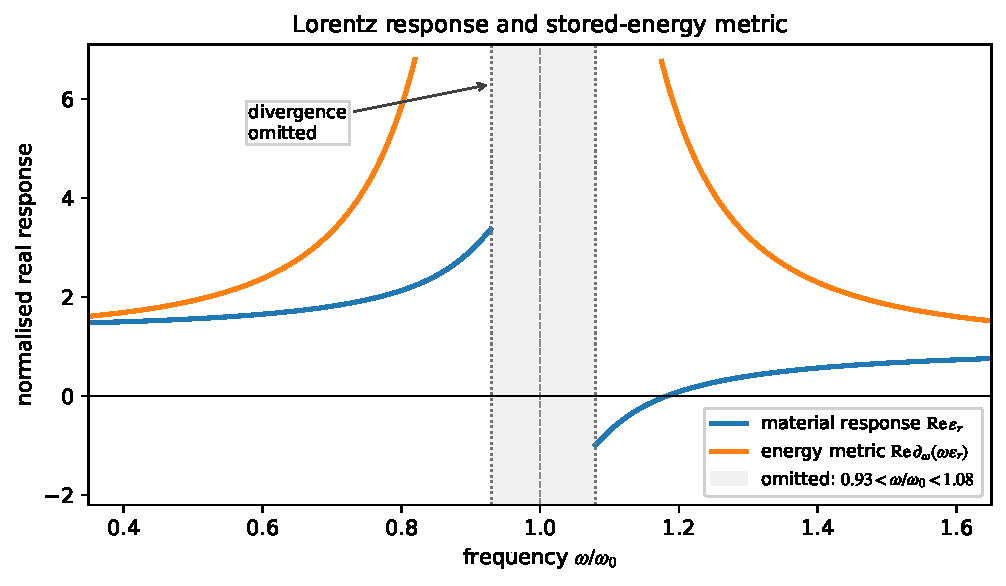
\includegraphics[width=0.82\textwidth]{figures/fig_ch03_energy_metric.pdf}
  \caption{A dispersive material illustrates why the electromagnetic
  inner product uses the energy derivative $\partial_\omega[\omega\varepsilon]$
  rather than the static permittivity alone.  Near a material resonance,
  the static response and the positive-energy metric can differ strongly.}
  \label{fig:ch03-energy-metric}
\end{figure}

\section*{Exercises}

\begin{exercise}
  For a uniform medium with $\Mmat=\diag(\varepsilon_0\varepsilon,
  \varepsilon_0\varepsilon,\varepsilon_0\varepsilon,
  \mu_0\mu,\mu_0\mu,\mu_0\mu)$, compute $\Mmat^{1/2}$ explicitly and
  verify that the energy-weighted operator
  $\tilde{\Hamop}=\Mmat^{-1/2}\Maxop(\kvec)\Mmat^{-1/2}$ is Hermitian
  by direct matrix computation for $\kvec=k\hat{z}$.
\end{exercise}

\begin{exercise}
  Consider a Drude plasma with $\varepsilon(\omega)=1-\omega_p^2/\omega^2$
  and $\mu=1$.  Compute the energy metric $\Mgmat(\omega)$ and verify
  that it is positive definite for $\omega>\omega_p$.  What happens at
  $\omega=\omega_p$?  Interpret physically.
\end{exercise}

\begin{exercise}
  For the gyrotropic permeability \eqref{eq:ch2-gyrotropic-mu}, suppose
  that $\mu_\perp(\omega)$, $\kappa(\omega)$, and $\mu_z(\omega)$ are
  given by the Polder model for a magnetised ferrite:
  \begin{equation}
    \mu_\perp = 1 + \frac{\omega_0\omega_m}{\omega_0^2-\omega^2}\,,
    \qquad
    \kappa = \frac{\omega\omega_m}{\omega_0^2-\omega^2}\,,
    \qquad
    \mu_z = 1\,,
  \end{equation}
  where $\omega_0$ is the Larmor frequency and $\omega_m$ is the
  saturation-magnetisation frequency.  Compute the $\mut$-block of
  $\Mgmat(\omega)$ and determine the frequency range over which it is
  positive definite.
\end{exercise}

\begin{exercise}
  Prove that in a periodic medium with Bloch boundary conditions, the
  surface integral in \eqref{eq:ch3-boundary-term} vanishes.
  \emph{Hint:} pair opposite faces of the unit cell and use the
  Bloch phase relation
  $\emfield(\rvec+\avec)=\ee^{\ii\kvec\cdot\avec}\emfield(\rvec)$.
\end{exercise}

\begin{exercise}[Longitudinal modes]
  Show that in a homogeneous isotropic medium, the six-component fields
  $\emfield_L=(\nabla\phi,\mathbf{0})^T$ (for arbitrary scalar $\phi$)
  and $\emfield_L'=(\mathbf{0},\nabla\psi)^T$ satisfy
  $\Maxop\emfield_L=0$ and $\Maxop\emfield_L'=0$.  Verify that they
  are orthogonal to every transverse mode under $\langle\cdot,\cdot\rangle_\Mmat$.
\end{exercise}

\begin{exercise}
  The dispersive inner product $\langle\cdot,\cdot\rangle_{\Mgmat}$
  involves $\Mgmat(\omega_n)$ evaluated at the eigenfrequency of mode~$n$.
  Show that for two degenerate modes at the same frequency
  ($\omega_n=\omega_m$), the inner product is well defined and reduces to
  the ordinary Hermitian form $\int\mathbf{u}_n^\dagger\Mgmat\mathbf{u}_m\,\dd^3r$.
\end{exercise}


\chapter{Periodic Media and Photonic Bands}
\label{ch:periodic-media}
% ======================================================================
%  Chapter 4 — Periodic Media and Photonic Bands
% ======================================================================

\section{Periodicity in optics}
\label{sec:ch4-periodicity}

A photonic crystal is a medium whose material matrix is periodic:
\begin{equation}\label{eq:ch4-periodicity}
  \Mmat(\rvec + \avec_i) = \Mmat(\rvec)
  \qquad\text{for lattice vectors } \avec_1, \avec_2, \avec_3\,.
\end{equation}
In two dimensions, the periodicity is in the $(\avec_1,\avec_2)$ plane
and $\Mmat$ is independent of $z$ (or periodic with a different period
in $z$); in one dimension, a single $\avec_1$ suffices.  This chapter
focuses on the two-dimensional case, which is the most important for
topological photonics, but the formalism applies in any dimension.

The physical origin of the periodicity can be a lattice of dielectric
rods, a pattern of holes in a slab, a structured metallic or ferrite
arrangement, or any other design in which the optical properties repeat.
What matters for the mathematics is only the discrete translational
symmetry \eqref{eq:ch4-periodicity}.

\section{Bloch's theorem for Maxwell modes}
\label{sec:ch4-bloch}

\subsection{Statement and proof}
\label{sec:ch4-bloch-statement}

\begin{theorem}[Bloch's theorem for electromagnetic fields]
  \label{thm:ch4-bloch}
  Let $\Mmat(\rvec)$ be periodic with lattice vectors $\{\avec_i\}$.
  Then every eigenmode of the Maxwell operator can be written in the
  Bloch form
  \begin{equation}\label{eq:ch4-bloch-form}
    \emfield_{n\kvec}(\rvec)
    = \ee^{\ii\kvec\cdot\rvec}\,\mathbf{u}_{n\kvec}(\rvec)\,,
  \end{equation}
  where $\kvec$ is the Bloch wavevector, $n$ is the band index, and
  $\mathbf{u}_{n\kvec}(\rvec)$ is cell-periodic:
  \begin{equation}\label{eq:ch4-cell-periodic}
    \mathbf{u}_{n\kvec}(\rvec+\avec_i)
    = \mathbf{u}_{n\kvec}(\rvec)
    \qquad\text{for all lattice vectors } \avec_i\,.
  \end{equation}
\end{theorem}

\begin{proof}
Define the translation operator $T_\avec$ by
$(T_\avec\emfield)(\rvec)=\emfield(\rvec+\avec)$.  Since
$\Mmat(\rvec+\avec)=\Mmat(\rvec)$, the Maxwell operator
$\Hamop(\rvec)=\Mmat^{-1}(\rvec)\Maxop$ commutes with $T_\avec$:
\begin{equation}
  [T_\avec,\,\Hamop] = 0
  \qquad\text{for all lattice vectors } \avec\,.
\end{equation}
The translation operators for different lattice vectors also commute
among themselves.  Therefore $\Hamop$ and $\{T_\avec\}$ can be
simultaneously diagonalised.

The eigenvalues of $T_\avec$ on a square-integrable (or Bloch-periodic)
function space are of the form
$T_\avec\emfield=\ee^{\ii\kvec\cdot\avec}\emfield$,
parametrised by a wavevector $\kvec$.  This is because $T_\avec$ is
unitary and the group of translations is Abelian, so its irreducible
representations are one-dimensional and given by characters
$\avec\mapsto\ee^{\ii\kvec\cdot\avec}$.

A simultaneous eigenfunction of $\Hamop$ and $T_\avec$ therefore
satisfies $\emfield(\rvec+\avec)=\ee^{\ii\kvec\cdot\avec}\emfield(\rvec)$.
Writing $\emfield(\rvec)=\ee^{\ii\kvec\cdot\rvec}\mathbf{u}(\rvec)$,
this condition becomes $\mathbf{u}(\rvec+\avec)=\mathbf{u}(\rvec)$:
$\mathbf{u}$ is cell-periodic.
\end{proof}

\subsection{The Brillouin zone}
\label{sec:ch4-bz}

The Bloch wavevector $\kvec$ is defined modulo reciprocal lattice
vectors $\Gvec$
\cite{initio2026pdf}.  Two wavevectors $\kvec$ and $\kvec+\Gvec$ label the
same physical mode (with a different choice of cell-periodic part), so
$\kvec$ can be restricted to a fundamental domain of the reciprocal
lattice---the \emph{first Brillouin zone} $\BZ$.

For a two-dimensional square lattice with period $a$, the reciprocal
lattice vectors are $\Gvec=\frac{2\pi}{a}(m_1\hat{x}+m_2\hat{y})$ and
the Brillouin zone is the square
$|k_x|,|k_y|\leq\pi/a$.  For a hexagonal lattice (which will be
central to the Dirac-cone physics of \chref{ch:dirac-cones}), the
Brillouin zone is a regular hexagon.

\begin{remark}[Topology of the Brillouin zone]
  The identification $\kvec\sim\kvec+\Gvec$ means that the Brillouin
  zone is topologically a \emph{torus} $T^2$ in two dimensions (or
  $T^3$ in three).  This closed, boundary-free topology is essential
  for the quantisation of the Chern number: the integral of the Berry
  curvature over a torus is always an integer multiple of $2\pi$
  (\chref{ch:geometry-bands}).
\end{remark}

\section{The cell-periodic eigenvalue problem}
\label{sec:ch4-cell-evp}

Substituting the Bloch form \eqref{eq:ch4-bloch-form} into the Maxwell
eigenvalue equation $\Maxop\emfield=\omega\Mmat\emfield$ and noting
that $\nabla(\ee^{\ii\kvec\cdot\rvec}\mathbf{u})
=\ee^{\ii\kvec\cdot\rvec}(\nabla+\ii\kvec)\mathbf{u}$, we obtain the
\emph{cell-periodic eigenvalue problem}:
\begin{equation}\label{eq:ch4-cell-evp}
  \boxed{%
  \Maxop(\kvec)\,\mathbf{u}_{n\kvec}(\rvec)
  = \omega_{n\kvec}\,\Mmat(\rvec)\,\mathbf{u}_{n\kvec}(\rvec)\,,}
\end{equation}
where the $\kvec$-dependent curl operator is
\begin{equation}\label{eq:ch4-maxop-k}
  \Maxop(\kvec) =
  \begin{pmatrix}
    \mathbf{0} & \ii(\nabla+\ii\kvec)\times \\[2pt]
    -\ii(\nabla+\ii\kvec)\times & \mathbf{0}
  \end{pmatrix}.
\end{equation}
This operator acts on cell-periodic functions and is parametrised by
$\kvec$.

The inner product for \eqref{eq:ch4-cell-evp} is the electromagnetic
inner product restricted to one unit cell $\Omega$:
\begin{equation}\label{eq:ch4-cell-ip}
  \left\langle \mathbf{u}_1,\mathbf{u}_2\right\rangle_{\Mmat,\Omega}
  = \int_\Omega
  \mathbf{u}_1^\dagger(\rvec)\,\Mmat(\rvec)\,
  \mathbf{u}_2(\rvec)\,\dd^d r\,.
\end{equation}
By the self-adjointness of $\Maxop(\kvec)$ under periodic boundary
conditions (Theorem~\ref{thm:ch3-self-adjoint}), the eigenfrequencies
$\omega_{n\kvec}$ are real and the cell-periodic eigenmodes are
orthogonal:
\begin{equation}\label{eq:ch4-cell-orth}
  \left\langle \mathbf{u}_{n\kvec},\mathbf{u}_{m\kvec}\right\rangle_{\Mmat,\Omega}
  = \delta_{nm}\,.
\end{equation}

\section{Band structure}
\label{sec:ch4-bands}

For each $\kvec$ in the Brillouin zone, the cell-periodic eigenvalue
problem \eqref{eq:ch4-cell-evp} has a discrete set of eigenfrequencies
\begin{equation}
  0 < \omega_{1\kvec} \leq \omega_{2\kvec} \leq \omega_{3\kvec}
  \leq \cdots\,.
\end{equation}
As $\kvec$ varies continuously over the Brillouin zone, each
$\omega_{n\kvec}$ traces out a continuous curve---the $n$-th
\emph{photonic band}.  The collection of all bands is the
\emph{photonic band structure} \cite{wu2015scheme,paz2019tutorial,ho1990existence}.

\subsection{Band gaps}
\label{sec:ch4-band-gaps}

A \emph{photonic band gap} is a frequency range
$(\omega_{\mathrm{low}},\omega_{\mathrm{high}})$ in which no
eigenfrequency exists for any $\kvec$ in the Brillouin zone:
\begin{equation}
  \max_\kvec\omega_{n\kvec} < \omega_{\mathrm{low}}
  < \omega_{\mathrm{high}}
  < \min_\kvec\omega_{(n+1)\kvec}\,
\end{equation}
The displayed formula above follows the convention and normalisation used in \cite{wang2007reflection}.
The existence and width of band gaps depend on the contrast of
$\Mmat(\rvec)$ between different regions of the unit cell and on the
lattice geometry.  High dielectric contrast and connected
high-$\varepsilon$ regions generally favour wider gaps.

Band gaps are essential for topological photonics: the Chern number of a
set of bands is well defined only when those bands are separated from
all others by gaps.  The topological edge states live inside these
gaps.

\subsection{Group velocity and energy velocity}
\label{sec:ch4-velocity}

The group velocity of the $n$-th band is
\begin{equation}\label{eq:ch4-group-velocity}
  \mathbf{v}_{g,n}(\kvec)
  = \nabla_\kvec\,\omega_{n\kvec}\,
\end{equation}
The displayed formula above follows the convention and normalisation used in \cite{raghu2008analogs}.
This can be evaluated using the Hellmann--Feynman theorem
\cite{haldane2008reflection}.
Differentiating the eigenvalue equation
$\Maxop(\kvec)\mathbf{u}_n=\omega_n\Mmat\mathbf{u}_n$ with respect to
$k_\alpha$ and taking the inner product with $\mathbf{u}_n$:
\begin{equation}\label{eq:ch4-hellmann-feynman}
  \pderiv{\omega_n}{k_\alpha}
  = \frac{
    \displaystyle\int_\Omega\mathbf{u}_n^\dagger\,
    \pderiv{\Maxop(\kvec)}{k_\alpha}\,\mathbf{u}_n\,\dd^d r
  }{
    \displaystyle\int_\Omega\mathbf{u}_n^\dagger\,\Mmat\,
    \mathbf{u}_n\,\dd^d r
  }\,.
\end{equation}
The numerator involves the $k_\alpha$-derivative of $\Maxop(\kvec)$,
which from \eqref{eq:ch4-maxop-k} has the structure of a ``velocity
operator'' coupling $\Efield$ and $\Hfield$ components.

The \emph{energy velocity} is defined as the ratio of time-averaged
Poynting flux to time-averaged energy:
\begin{equation}\label{eq:ch4-energy-velocity}
  \mathbf{v}_E
  = \frac{\int_\Omega\langle\Sfield\rangle\,\dd^d r}
         {\int_\Omega\langle u\rangle\,\dd^d r}\,.
\end{equation}
In a lossless nondispersive medium, one can show that
$\mathbf{v}_g=\mathbf{v}_E$ by combining the Hellmann--Feynman relation
with Poynting's theorem.  In a dispersive medium, the equality
$\mathbf{v}_g=\mathbf{v}_E$ still holds provided the energy density
is computed using the dispersive metric $\Mgmat$.

\section{TE and TM modes in two dimensions}
\label{sec:ch4-te-tm}

For a two-dimensional photonic crystal with $\Mmat$ independent of $z$
and no propagation in the $z$-direction ($k_z=0$), the six-component
eigenproblem separates into two independent scalar problems.

\subsection{TM polarisation}
\label{sec:ch4-tm}

The TM modes have $\Efield=E_z\hat{z}$ and
$\Hfield=(H_x,H_y,0)^T$.  The curl equations reduce to a single
scalar equation for $E_z$:
\begin{equation}\label{eq:ch4-tm-scalar}
  -(\nabla+\ii\kvec_\parallel)\cdot\bigl[
    \mut^{-1}(\rvec)\,(\nabla+\ii\kvec_\parallel)E_z(\rvec)
  \bigr]
  = \frac{\omega^2}{c^2}\,\varepsilon_{zz}(\rvec)\,E_z(\rvec)\,,
\end{equation}
where $\kvec_\parallel=(k_x,k_y)$ and $\mut^{-1}$ is the $2\times 2$
in-plane inverse permeability tensor.

For an isotropic nonmagnetic medium ($\mut=\mathbf{I}$), this
simplifies to the standard TM eigenproblem:
\begin{equation}\label{eq:ch4-tm-simple}
  -(\nabla+\ii\kvec_\parallel)^2 E_z(\rvec)
  = \frac{\omega^2}{c^2}\,\varepsilon(\rvec)\,E_z(\rvec)\,.
\end{equation}

\subsection{TE polarisation}
\label{sec:ch4-te}

The TE modes have $\Hfield=H_z\hat{z}$ and
$\Efield=(E_x,E_y,0)^T$.  The scalar equation is
\begin{equation}\label{eq:ch4-te-scalar}
  -(\nabla+\ii\kvec_\parallel)\cdot\bigl[
    \epst^{-1}(\rvec)\,(\nabla+\ii\kvec_\parallel)H_z(\rvec)
  \bigr]
  = \frac{\omega^2}{c^2}\,\mu_{zz}(\rvec)\,H_z(\rvec)\,.
\end{equation}

\subsection{Gyrotropic media: coupling through off-diagonal terms}
\label{sec:ch4-gyrotropic}

When the permeability tensor has off-diagonal gyrotropic components as
in \eqref{eq:ch2-gyrotropic-mu}, the inverse permeability
\begin{equation}\label{eq:ch4-mu-inv}
  \mut_\perp^{-1}
  = \frac{1}{\mu_\perp^2-\kappa^2}
  \begin{pmatrix}
    \mu_\perp & \ii\kappa \\
    -\ii\kappa & \mu_\perp
  \end{pmatrix}
\end{equation}
introduces first-order spatial derivatives through the off-diagonal
gyrotropic elements.  The correct operator form retains the full
tensor contraction with spatially varying coefficients:
\begin{equation}\label{eq:ch4-tm-gyrotropic}
  -D_i\bigl[(\mu^{-1})_{ij}(\rvec)\,D_j E_z\bigr]
  = \frac{\omega^2}{c^2}\,\varepsilon(\rvec)\,E_z\,,
  \qquad D_i\equiv\partial_i+\ii k_i\,,
\end{equation}
where $i,j\in\{x,y\}$ and summation over repeated indices is implied.
For a uniform gyrotropic medium, the off-diagonal elements of
$(\mu^{-1})_{ij}$ contribute through the commutator
$D_i D_j - D_j D_i=0$ (for constant $\kvec$), so the gyrotropic
coupling vanishes.  The physically important gyrotropic effect arises
from the \emph{spatial variation} of $(\mu^{-1})_{ij}(\rvec)$ at
material interfaces, where the differential operator does not commute
with the position-dependent tensor.  This spatially varying gyrotropic
coupling breaks the symmetry $\kvec\to-\kvec$ and is responsible for
the nonzero Berry curvature analysed in \chref{ch:breaking-tr}.

\begin{remark}
In the gyrotropic case, the TE and TM polarisations are not strictly
decoupled when $\kappa\neq 0$ and the geometry mixes in-plane and
out-of-plane components.  However, for a 2D crystal with
$\epst$ diagonal and $\mut$ of the form
\eqref{eq:ch2-gyrotropic-mu}, the TM and TE sectors remain
exactly separated at $k_z=0$.  This separation is exploited in all the
standard topological photonic-crystal designs.
\end{remark}

\section{The plane-wave expansion}
\label{sec:ch4-pwe}

The most widely used method for computing photonic band structures is
the plane-wave expansion (PWE) \cite{ozawa2018topological,haldane2008possible,initio2026pdf}, in which the cell-periodic fields and
material parameters are expanded in Fourier series over reciprocal
lattice vectors.

\subsection{Fourier expansion of fields and material parameters}
\label{sec:ch4-fourier}

Expand the cell-periodic field in a Fourier series:
\begin{equation}\label{eq:ch4-fourier-field}
  \mathbf{u}_{n\kvec}(\rvec)
  = \sum_\Gvec \hat{\mathbf{u}}_{n\kvec}(\Gvec)\,
    \ee^{\ii\Gvec\cdot\rvec}\,,
\end{equation}
and similarly for the material parameters:
\begin{equation}\label{eq:ch4-fourier-eps}
  \varepsilon(\rvec) = \sum_\Gvec \hat{\varepsilon}(\Gvec)\,
    \ee^{\ii\Gvec\cdot\rvec}\,,
  \qquad
  \mu^{-1}(\rvec) = \sum_\Gvec \widehat{\mu^{-1}}(\Gvec)\,
    \ee^{\ii\Gvec\cdot\rvec}\,.
\end{equation}
The Fourier coefficients are computed from integrals over the unit cell:
\begin{equation}\label{eq:ch4-fourier-coeff}
  \hat{\varepsilon}(\Gvec)
  = \frac{1}{A_\Omega}\int_\Omega
    \varepsilon(\rvec)\,\ee^{-\ii\Gvec\cdot\rvec}\,\dd^2 r\,,
\end{equation}
where $A_\Omega$ is the area of the 2D unit cell.

\subsection{Matrix eigenvalue problem}
\label{sec:ch4-matrix-evp}

Substituting the Fourier expansions into the TM eigenvalue equation
\eqref{eq:ch4-tm-scalar}, the convolution of material parameters and
\begin{equation}\label{eq:ch4-pwe-matrix}
  \sum_{\Gvec'}
  (\kvec+\Gvec)_i\,
  \widehat{(\mu^{-1})_{ij}}(\Gvec-\Gvec')\,
  (\kvec+\Gvec')_j\,\hat{E}_z(\Gvec')
  = \frac{\omega^2}{c^2}\sum_{\Gvec'}
    \hat{\varepsilon}(\Gvec-\Gvec')\,\hat{E}_z(\Gvec')\,,
\end{equation}
where summation over repeated Cartesian indices $i,j\in\{x,y\}$ is
implied.  For a scalar (non-gyrotropic) inverse permeability, the
tensor Fourier coefficient reduces to
$\widehat{(\mu^{-1})_{ij}}(\Gvec)=\widehat{\mu^{-1}}(\Gvec)\,
\delta_{ij}$ and the left-hand side simplifies to
$(\kvec+\Gvec)\cdot(\kvec+\Gvec')\,\widehat{\mu^{-1}}(\Gvec-\Gvec')$.
For gyrotropic media, the off-diagonal Fourier components
$\widehat{(\mu^{-1})_{xy}}$ carry the topological information.
In practice, the Fourier series is truncated to $N_G$ reciprocal
lattice vectors, yielding an $N_G\times N_G$ generalised Hermitian
matrix eigenvalue problem at each $\kvec$ point.  The eigenvalues
$\omega_{n\kvec}^2/c^2$ give the band structure; the eigenvectors give
the mode profiles.
$\omega_{n\kvec}^2/c^2$ give the band structure; the eigenvectors give
the mode profiles.

\begin{remark}[Convergence]
  The PWE converges exponentially fast for smooth material profiles and
  algebraically for discontinuous profiles (e.g.\ circular rods).  For
  the latter, careful treatment of the Fourier factorisation (the
  ``inverse rule'' of Li) is needed to avoid slow convergence \cite{raman2010photonic}.  We
  discuss numerical methods further in \chref{ch:computing-chern} and
  \appref{app:numerical-recipes}.
\end{remark}

\section{Examples of photonic band structures}
\label{sec:ch4-examples}

\subsection{Square lattice of dielectric rods}
\label{sec:ch4-square-rods}

Consider a two-dimensional square lattice (period $a$) of circular
dielectric rods (radius $r$, permittivity $\varepsilon_r$) in air
($\varepsilon=1$), with $\mu=1$ everywhere.  This is the standard
textbook photonic crystal.

For TM polarisation, the lowest bands emerge from the folding of the
free-photon dispersion $\omega=c|\kvec+\Gvec|$ at the Brillouin-zone
boundaries.  When the dielectric contrast $\varepsilon_r/1$ is
sufficiently large ($\varepsilon_r\gtrsim 8$ for $r/a\approx 0.2$), a
\emph{complete TM band gap} opens between the first and second bands.

A representative TM band structure for this system, computed by the
plane-wave expansion method with $\varepsilon_r=12$ and $r/a=0.2$,
shows a complete TM gap between the first and second bands spanning
approximately $15\%$ of the mid-gap frequency.  The gap arises because
the first band concentrates its electric field energy in the
high-permittivity rods, while the second band is forced by
orthogonality to concentrate in the low-permittivity air region,
paying a higher electromagnetic energy cost.  This concentration
mechanism---known as the ``dielectric'' and ``air'' band distinction
in the photonic crystal literature---is the spatial analog of the
bonding/anti-bonding splitting in electronic band theory.

\subsection{Hexagonal lattice and Dirac points}
\label{sec:ch4-hex-dirac}

The hexagonal (triangular) lattice is particularly important for
topological photonics.  At the corners $K$ and $K'$ of the hexagonal
Brillouin zone, the $C_{6v}$ point-group symmetry can enforce
\emph{Dirac-point degeneracies}: pairs of bands that touch linearly,
with a dispersion relation locally resembling that of massless
relativistic fermions:
\begin{equation}\label{eq:ch4-dirac-dispersion}
  \omega_\pm(\kvec) \approx \omega_D \pm v_D|\delta\kvec|\,,
\end{equation}
where $\delta\kvec=\kvec-\kvec_D$ is the displacement from the Dirac
point, $\omega_D$ is the Dirac frequency, and $v_D$ is the Dirac
velocity.

These Dirac points are the starting point for topological gap opening:
when time-reversal symmetry is broken by a gyrotropic perturbation, the
degeneracy is lifted and the resulting gapped bands acquire nonzero
Chern numbers.  This is the subject of Chapters~\ref{ch:dirac-cones}
and \ref{ch:breaking-tr}.

\section{Symmetry and degeneracy}
\label{sec:ch4-symmetry}

The symmetries of the photonic crystal---both spatial (point group,
space group) and non-spatial (time reversal)---constrain the band
structure and the allowed degeneracies.

\subsection{Point-group symmetry}
\label{sec:ch4-point-group}

At high-symmetry points in the Brillouin zone, the little group
(the subgroup of the point group that leaves $\kvec$ invariant) determines
the allowed irreducible representations of the eigenmodes.  Bands that
belong to multi-dimensional representations are degenerate.

For example, at the $\Gamma$ point ($\kvec=\mathbf{0}$) of a
$C_{6v}$-symmetric hexagonal lattice, the modes transform under the
full $C_{6v}$ group and can be labelled by the irreducible
representations $A_1$, $A_2$, $B_1$, $B_2$, $E_1$, $E_2$.  The
two-dimensional representations $E_1$ and $E_2$ correspond to doubly
degenerate modes.

\subsection{Time reversal and the dispersion relation}
\label{sec:ch4-tr-dispersion}

When the medium is time-reversal invariant (reciprocal, $\kappa=0$),
the Bloch eigenfrequencies satisfy
\begin{equation}\label{eq:ch4-tr-symmetry}
  \omega_n(\kvec) = \omega_n(-\kvec)\,.
\end{equation}
This is a direct consequence of the time-reversal symmetry derived in
\secref{sec:ch2-time-reversal}: if $\mathbf{u}_{n\kvec}$ is an
eigenmode at $\kvec$, then $\Top\mathbf{u}_{n\kvec}$ is an eigenmode at
$-\kvec$ with the same frequency.

Breaking time-reversal symmetry ($\kappa\neq 0$) allows
$\omega_n(\kvec)\neq\omega_n(-\kvec)$.  This asymmetry is directly
visible in the band structure as a tilt or splitting at time-reversal-related
points, and it is the physical origin of nonreciprocal wave propagation.

\subsection{Inversion symmetry and band sticking}
\label{sec:ch4-inversion}

When the photonic crystal has inversion symmetry
($\Mmat(-\rvec)=\sigma_z\Mmat(\rvec)\sigma_z$), the eigenfrequencies
satisfy $\omega_n(\kvec)=\omega_n(-\kvec)$ \emph{independently} of
time-reversal symmetry.  The combined effect of inversion and
time-reversal symmetry can force additional degeneracies at
high-symmetry points, which is important for the formation of
Dirac points.

\section{From bands to topology}
\label{sec:ch4-bands-to-topology}

The photonic band structure $\{\omega_n(\kvec)\}$ tells us
\emph{where} light can propagate: inside bands, at the corresponding
frequencies and wavevectors.  But the band structure alone does not tell
the full story.  Two photonic crystals can have identical band
structures---the same frequencies, the same gaps---and yet differ in a
fundamental way that affects their interface physics.

The missing information is the \emph{geometry of the eigenmodes} as
functions of $\kvec$.  As $\kvec$ traverses the Brillouin zone, the
cell-periodic mode $\mathbf{u}_{n\kvec}(\rvec)$ rotates in the
Hilbert space of cell-periodic fields.  The rate and manner of this
rotation are captured by the Berry connection and Berry curvature,
which we derive in the next chapter.

The topological invariant---the Chern number---is an integer that
characterises the \emph{global} geometry of each band over the entire
Brillouin zone \cite{thouless1982quantized}.  It cannot be changed by any smooth deformation of the
medium that does not close the band gap.  When two media with different
Chern numbers are brought together, the mismatch forces the existence
of interface modes that cross the gap: these are the topological edge
states.

\section{Group velocity and the Maxwell Hellmann--Feynman theorem}
\label{sec:ch4-group-velocity}

The group velocity of a Bloch mode is the gradient of the band
frequency with respect to the wavevector:
$\mathbf{v}_g=\nabla_\kvec\omega_n(\kvec)$.  This can be computed
directly from the eigenvalue equation by a Hellmann--Feynman argument.

Differentiating the Bloch eigenproblem
$\Maxop(\kvec)\mathbf{u}_{n\kvec}
=\omega_{n\kvec}\Mmat\mathbf{u}_{n\kvec}$ with respect to $k_a$
and projecting onto $\mathbf{u}_{n\kvec}$ gives
\cite{gangaraj2016berry,ozawa2018topological}
\begin{equation}\label{eq:ch4-hellmann-feynman-group}
  v_{g,a}
  = \frac{\partial\omega_n}{\partial k_a}
  = \frac{\displaystyle\int_{\mathrm{cell}}
    \mathbf{u}_n^\dagger\,(\partial_{k_a}\Maxop)\,
    \mathbf{u}_n\,\dd^3r}
  {\displaystyle\int_{\mathrm{cell}}
    \mathbf{u}_n^\dagger\,\Mmat\,\mathbf{u}_n\,\dd^3r}\,,
\end{equation}
where the numerator uses the \emph{unweighted} $L^2$ matrix element
of the velocity operator $\partial_{k_a}\Maxop$ and the denominator
is the energy normalisation $\int\mathbf{u}_n^\dagger\Mmat\mathbf{u}_n\,\dd^3r$.

For a non-dispersive medium, this reduces to the ratio of the
time-averaged Poynting flux to the energy density, as expected from
energy-transport arguments.  For dispersive media, the denominator
must use the dispersive metric $\Mgmat$ instead of $\Mmat$, giving the
group velocity in terms of the Brillouin energy.

The Hellmann--Feynman formula is the starting point for the
$\kvec\cdot\mathbf{p}$ perturbation theory used in
Chapter~\ref{ch:dirac-cones} to derive the Dirac velocity at
photonic Dirac points.

\subsection{Density of states and van Hove singularities}
\label{sec:ch4-dos}

The photonic density of states is defined as
$\rho(\omega)=\sum_n\int_{\mathrm{BZ}}
\delta(\omega-\omega_n(\kvec))\,\dd^d k/(2\pi)^d$.
In two dimensions, $\rho(\omega)$ has logarithmic van Hove
singularities at frequencies where $\nabla_\kvec\omega_n=0$
(band extrema and saddle points).  These singularities are important
for understanding the spontaneous emission rate of emitters
in photonic crystals and for identifying the frequencies at which
strong light--matter interaction can be expected
\cite{ozawa2018topological}.

Near a Dirac point (Chapter~\ref{ch:dirac-cones}), the conical
dispersion gives a density of states
$\rho(\omega)\propto|\omega-\omega_D|/v_D^2$ that vanishes linearly,
analogous to graphene.  Inside a complete band gap,
$\rho(\omega)=0$---no propagating states exist, and the gap frequency
range is available for topological edge modes.

\section{Conditions for a complete photonic band gap}
\label{sec:ch4-complete-gap}

A complete photonic band gap---a frequency range with no propagating
modes for any polarisation and any wavevector direction---requires
both sufficiently large dielectric contrast and the right lattice
symmetry.

For a 2D photonic crystal, the TE and TM polarisations are decoupled
(Section~\ref{sec:ch4-te-tm}), and each polarisation has its own gap.
A TE gap requires connected dielectric regions (veins), while a TM gap
requires isolated high-$\varepsilon$ regions (rods).  A complete 2D
gap (for both polarisations simultaneously) therefore requires a
structure that is simultaneously connected and has isolated
high-$\varepsilon$ regions, which is possible in certain lattice
geometries (e.g.\ the honeycomb lattice with thick veins and
additional rods) \cite{haldane2008possible}.

For 3D photonic crystals, complete gaps are harder to achieve because
the gap must survive for all propagation directions and both
polarisations.  Diamond and gyroid lattice symmetries provide the
largest complete 3D gaps, reaching up to $25\%$ of the mid-gap
frequency for germanium ($\varepsilon\approx 16$) at near-infrared
wavelengths \cite{price2022roadmap}.

The existence of a complete gap is a prerequisite for all topological
phenomena discussed in this book: the topological invariants are
defined for isolated bands, and the edge modes exist in the gap.
Without a gap, there is no topological protection.

\section{Photonic band structure computation in practice}
\label{sec:ch4-band-computation}

The computation of photonic band structures is a central practical
skill for topological photonics.  This section provides the
computational context that is developed in full algorithmic detail in
Appendix~\ref{app:numerical-recipes}.

\subsection{The plane-wave expansion method}
\label{sec:ch4-pwe-method}

The plane-wave expansion (PWE) method expands the cell-periodic fields
$\mathbf{u}_{n\kvec}(\rvec)$ in Fourier harmonics
$\ee^{\ii\mathbf{G}\cdot\rvec}$, where $\mathbf{G}$ ranges over
reciprocal lattice vectors.  The Bloch eigenvalue problem becomes a
matrix eigenvalue problem of dimension $6N_G$ (or $2N_G$ for a single
polarisation in 2D), where $N_G$ is the number of plane waves
retained.

The convergence of the PWE method depends on the dielectric contrast:
for moderate contrast ($\varepsilon_r\lesssim 12$), convergence to
$0.1\%$ accuracy is typically achieved with $N_G\approx 100$--$200$
plane waves.  For high contrast ($\varepsilon_r>20$) or metallic
structures, the Gibbs phenomenon at material interfaces can slow
convergence, and supercell or finite-element methods may be preferable
\cite{ozawa2018topological,haldane2008possible}.

\subsection{High-symmetry paths and irreducible Brillouin zone}
\label{sec:ch4-high-symmetry}

The band structure is conventionally plotted along paths connecting
high-symmetry points of the Brillouin zone.  For the hexagonal
lattice used throughout this book, the high-symmetry points are
$\Gamma=(0,0)$, $M=(\pi/a,0)$, and $K=(4\pi/(3a),0)$, and the
standard path is $\Gamma\to M\to K\to\Gamma$.

The irreducible Brillouin zone (IBZ) is the smallest region that
generates the full BZ under the point-group symmetry operations.
For the hexagonal lattice with $C_{6v}$ symmetry, the IBZ is a
triangle $\Gamma$--$M$--$K$, which is $1/12$ of the full BZ.
Computing band structures and Berry curvatures over the IBZ and
extending by symmetry reduces the computational cost by a factor of
12 \cite{price2022roadmap,gangaraj2016berry}.

\section{Achieving a complete photonic band gap}
\label{sec:ch4-complete-gap-conditions}

A complete photonic band gap---a frequency range in which no
propagating mode exists for any wavevector and any polarisation---is
a prerequisite for confining light in all directions and for defining
topological edge modes that are truly isolated from the bulk
continuum.

\subsection{Necessary conditions}
\label{sec:ch4-gap-necessary}

For a 2D photonic crystal, a complete gap requires that the gap
for TE modes and the gap for TM modes overlap in frequency.  Since
TE gaps favour connected dielectric regions (``veins'') while TM gaps
favour isolated dielectric regions (``islands''), achieving a complete
gap requires a structure that simultaneously satisfies both
conditions.  The triangular lattice of air holes in a high-index
dielectric is a standard solution: the connected dielectric forms
veins for the TE gap, while the isolated dielectric regions between
the holes form effective islands for the TM gap
\cite{ozawa2018topological,haldane2008possible}.

The dielectric contrast must exceed a minimum threshold for a complete
gap to open.  For the triangular lattice, this threshold is
$\varepsilon_{\mathrm{max}}/\varepsilon_{\mathrm{min}}\gtrsim 4$ for
TE modes and $\gtrsim 7$ for a complete (TE+TM) gap.  Silicon
($\varepsilon_r\approx 11.7$) comfortably exceeds both thresholds,
making it the standard material for photonic crystal devices at
telecommunications wavelengths \cite{price2022roadmap}.

\subsection{Gap maps and structural optimisation}
\label{sec:ch4-gap-maps}

A gap map plots the gap width as a function of a structural parameter
(typically the hole radius $r/a$ or the filling fraction $f$).  The
optimal gap width for the triangular air-hole lattice occurs near
$r/a\approx 0.45$, $f\approx 0.73$, giving a complete gap of
$\Delta\omega/\omega_{\mathrm{mid}}\approx 20\%$.

For topological photonics, the relevant gap is not the largest
complete gap but the gap that opens at a band crossing (Dirac point or
quadratic touching) when a symmetry is broken.  These topological gaps
are typically much narrower ($1$--$5\%$) because they arise from a
perturbative splitting rather than from the fundamental photonic band
gap \cite{asbth2016berry,ozawa2018topological}.

\section{Photonic density of states and edge enhancement}
\label{sec:ch4-dos-van-hove}

The photonic density of states (DOS)
$\rho(\omega)=\sum_n\int_{\mathrm{BZ}}\delta(\omega-\omega_n(\kvec))
\,\dd^2 k/(2\pi)^2$ determines the local emission rate through
Fermi's golden rule and is a central quantity for light--matter
interaction in photonic crystals.

At a band edge, the group velocity
$\mathbf{v}_g=\nabla_\kvec\omega_n$ vanishes and the DOS diverges
as a van Hove singularity.  In 2D, the singularity is logarithmic:
$\rho(\omega)\sim -\ln|\omega-\omega_{\mathrm{edge}}|$ for a
quadratic band edge.  At a Dirac point, the linear dispersion gives
$\rho(\omega)\propto|\omega-\omega_D|$, which vanishes at the Dirac
frequency---a pseudogap.

When a topological gap opens at the Dirac point
(Chapter~\ref{ch:breaking-tr}), the pseudogap is replaced by a true
gap where $\rho(\omega)=0$ for $|\omega-\omega_D|<|\kappa|$.  The
gap edges acquire logarithmic van Hove singularities, producing
enhanced emission rates that can be exploited for cavity QED and
lasing applications \cite{ozawa2018topological,haldane2008possible}.

\subsection{Local density of states and edge enhancement}
\label{sec:ch4-ldos}

The local density of states (LDOS)
$\rho(\omega,\rvec)=\sum_n|\emfield_n(\rvec)|^2\,
\delta(\omega-\omega_n)$ depends on position and is directly
measurable through near-field spectroscopy.  At the boundary of a
topological photonic crystal, the LDOS has a contribution from the
edge mode that is absent in the bulk:
\begin{equation}\label{eq:ch4-ldos-edge}
  \rho_{\mathrm{edge}}(\omega,\rvec)
  = \frac{|\psi_0(\rvec)|^2}{2\pi v_g}\,,
  \quad \omega_D-|\kappa|<\omega<\omega_D+|\kappa|\,,
\end{equation}
where $\psi_0(\rvec)$ is the transverse edge-mode profile and $v_g$
is the edge-mode group velocity.  This edge-enhanced LDOS is
promising for single-photon sources: an emitter placed near the edge
of a topological crystal can emit predominantly into the
unidirectional edge mode, with a Purcell factor proportional to
$1/v_g$ \cite{price2022roadmap,gangaraj2016berry}.

\begin{figure}[t]
  \centering
  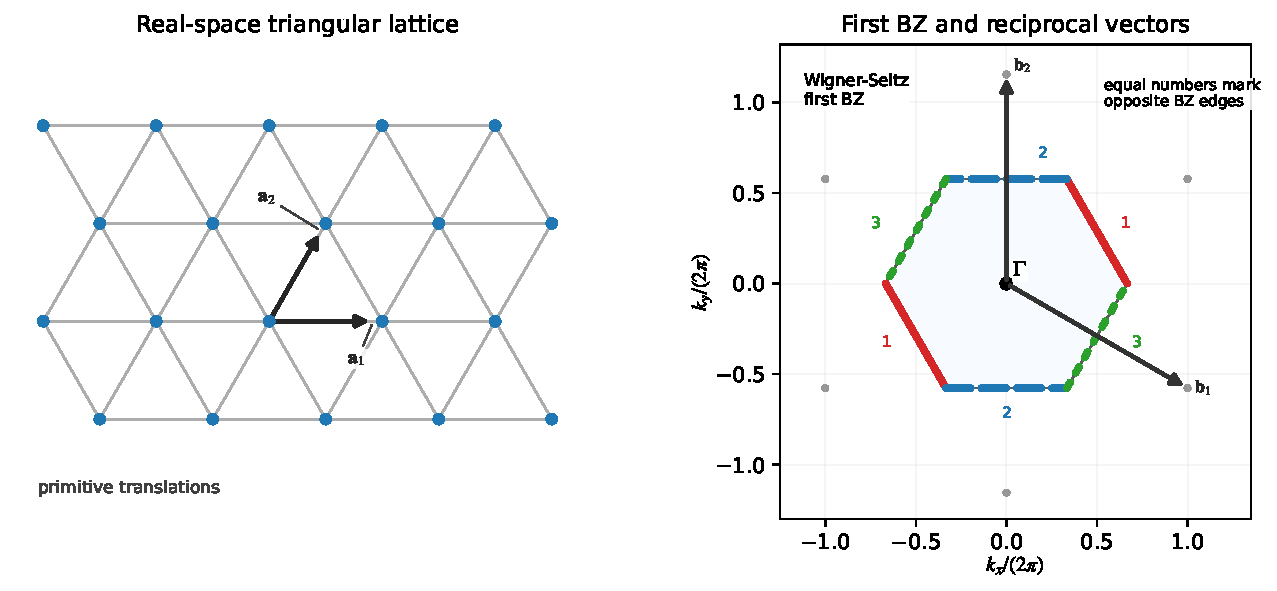
\includegraphics[width=0.88\textwidth]{figures/fig_ch04_bloch_brillouin.pdf}
  \caption{Real-space periodicity and reciprocal-space sewing.  Bloch
  theory replaces translation in the photonic crystal by a cell-periodic
  field on the Brillouin-zone torus; opposite BZ boundaries are identified
  by reciprocal-lattice phase factors, an issue that becomes important in
  numerical Chern computations.}
  \label{fig:ch04-bloch-brillouin}
\end{figure}

\section{Photonic band structure in practice}
\label{sec:ch4-practical-bands}

The Bloch theory and plane-wave expansion method developed in this
chapter provide the foundation for computing photonic band structures.
This section discusses practical aspects of band-structure
calculations that are important for topological photonics
applications.

\subsection{High-symmetry paths and the irreducible Brillouin zone}
\label{sec:ch4-high-symmetry-paths}

Band structures are conventionally plotted along high-symmetry
paths connecting special points of the Brillouin zone.  For the
triangular lattice (the most common lattice in topological photonics),
the standard path is $\Gamma\to M\to K\to\Gamma$, where
$\Gamma=(0,0)$, $M=\bvec_1/2$, and $K=(2\bvec_1+\bvec_2)/3$ in
reciprocal lattice coordinates.

The choice of path determines which band crossings and gaps are
visible in the band diagram.  In particular, Dirac cones at the $K$
and $K'$ points (Chapter~\ref{ch:dirac-cones}) are visible only if
the path passes through these points.  A common mistake is to plot
the band structure along $\Gamma\to X\to M\to\Gamma$ (the path
for a square lattice), which misses the Dirac cones entirely
\cite{press2026photonic,initio2026pdf}.

\subsection{Convergence with respect to plane waves}
\label{sec:ch4-pwe-convergence}

The plane-wave expansion method represents the periodic part of the
Bloch modes as a Fourier series truncated at $|\Gvec|\leq G_{\max}$.
The number of plane waves $N_G$ scales as $G_{\max}^d$ in $d$
dimensions, and the computational cost of diagonalisation scales
as $O(N_G^3)$.  For 2D photonic crystals, convergence of the lowest
bands typically requires $N_G \sim 100$--$500$, corresponding to
$G_{\max} \sim 5$--$10$ reciprocal lattice vectors.

The convergence rate depends on the dielectric contrast
$\varepsilon_{\max}/\varepsilon_{\min}$: higher contrast requires
more plane waves because the field variations are sharper.  For
the YIG photonic crystals of Chapter~\ref{ch:microwave-crystal}
($\varepsilon_{\mathrm{rod}}/\varepsilon_{\mathrm{air}} \approx 15$),
convergence to $<0.1\%$ accuracy in the eigenfrequencies requires
$N_G \gtrsim 300$ \cite{zhao2020first,press2026photonic}.

Figure~\ref{fig:ch04-pwe-convergence} illustrates the two key aspects of the
plane-wave expansion.  Panel~(a) shows the reciprocal-lattice vectors of a
triangular lattice, partitioned into a kept core (blue), an added convergence
shell (orange), and discarded higher-order vectors (grey).  The dashed circles
mark two values of the truncation radius $G_{\max}$; increasing $G_{\max}$
adds more plane waves but raises the matrix dimension.  Panel~(b) shows the
resulting convergence of a representative normalised eigenfrequency
$\omega a/2\pi c$ as the number of plane waves $N_G$ grows from~25
to~441.  The frequency approaches the independently computed reference value
(dotted line) from above, while the relative error (red, right axis,
$\log_{10}$ scale) decreases by more than two orders of magnitude.  In practice,
the discrete $N_G$ values correspond to successive circular truncation shells
of the reciprocal lattice.

\begin{figure}[t]
  \centering
  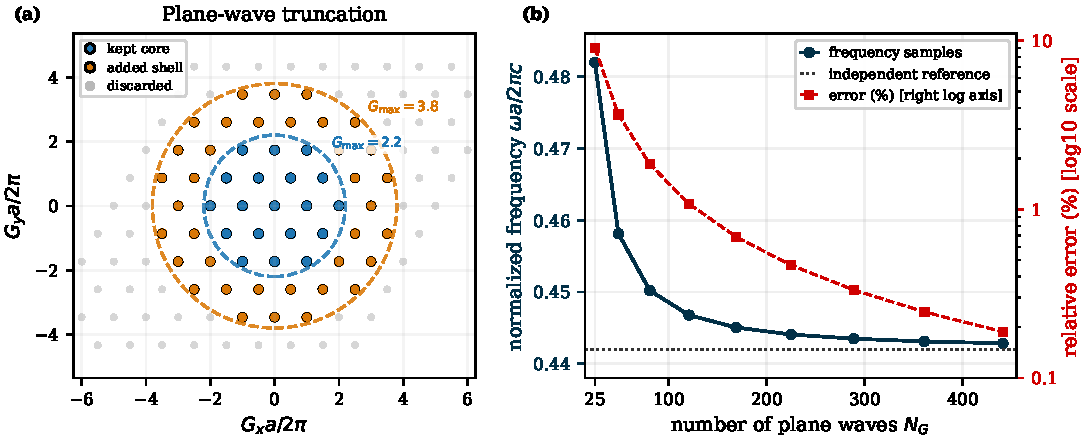
\includegraphics[width=0.95\textwidth]{figures/fig_ch04_pwe_convergence_step178.pdf}
  \caption{Plane-wave expansion in reciprocal space.
  (a)~Reciprocal-lattice vectors of a triangular lattice, classified as kept
  core (blue), added convergence shell (orange), or discarded (grey); dashed
  circles mark two truncation radii $G_{\max}$.
  (b)~Convergence of a normalised eigenfrequency as a function of the number
  of plane waves~$N_G$.  The right axis (red, $\log_{10}$ scale) shows the
  percent relative error with respect to the independently computed reference
  (dotted line).  Each data point corresponds to a successive circular
  truncation shell in reciprocal space.}
  \label{fig:ch04-pwe-convergence}
\end{figure}

\subsection{Supercell method for edge states}
\label{sec:ch4-supercell}

To compute edge-state dispersions, one uses a supercell that is
periodic in one direction (say $x$) and finite in the other ($y$).
The supercell contains a strip of the photonic crystal with the
topological material on one side and vacuum (or a trivially gapped
crystal) on the other.  The edge states appear as bands that cross
the bulk gap.

The supercell width $W$ must be large enough that the edge modes on
opposite boundaries do not hybridise (Section~\ref{sec:ch8-penetration-depth}).
For a topological gap of relative width $\Delta\omega/\omega \sim 3\%$,
a supercell of $\sim 15$--$20$ unit cells in the $y$-direction is
typically sufficient \cite{ozawa2018topological,paz2019tutorial}.

The supercell band structure provides the most direct verification of
the bulk-edge correspondence: one counts the number of edge modes
crossing the gap with positive group velocity and compares with the
bulk Chern number computed from the methods of
Chapter~\ref{ch:computing-chern}.

\section*{Exercises}

\begin{exercise}
  For a 1D photonic crystal (Bragg stack) with alternating layers of
  refractive indices $n_1$ and $n_2$ and thicknesses $d_1$ and $d_2$
  ($d_1+d_2=a$), derive the dispersion relation
  $\cos(ka)=\cos(n_1\omega d_1/c)\cos(n_2\omega d_2/c)
  -\frac{1}{2}(\frac{n_1}{n_2}+\frac{n_2}{n_1})
  \sin(n_1\omega d_1/c)\sin(n_2\omega d_2/c)$
  using the transfer-matrix method.  Identify the band gaps.
\end{exercise}

\begin{exercise}
  Show that the cell-periodic eigenvalue problem \eqref{eq:ch4-cell-evp}
  at $\kvec$ and $\kvec+\Gvec$ are unitarily related:
  $\mathbf{u}_{n,\kvec+\Gvec}(\rvec)
  =\ee^{-\ii\Gvec\cdot\rvec}\mathbf{u}_{n\kvec}(\rvec)$.
  Conclude that the band structure is periodic in $\kvec$.
\end{exercise}

\begin{exercise}
  Derive the Hellmann--Feynman formula \eqref{eq:ch4-hellmann-feynman}
  for the group velocity by differentiating the eigenvalue equation
  with respect to $k_\alpha$ and using the orthonormality of modes.
  Show that in a nondispersive medium the result agrees with the
  energy-velocity formula \eqref{eq:ch4-energy-velocity}.
\end{exercise}

\begin{exercise}
  For the TM modes of a 2D square lattice of circular rods, write out
  the plane-wave expansion matrix \eqref{eq:ch4-pwe-matrix} for the
  case $N_G=9$ (including $\Gvec=\frac{2\pi}{a}(m_1,m_2)$ with
  $m_1,m_2\in\{-1,0,1\}$).  Compute the Fourier coefficient
  $\hat\varepsilon(\Gvec)$ for a circular rod of radius $r$ and
  permittivity $\varepsilon_r$ in a unit cell of side $a$.
\end{exercise}

\begin{exercise}
  At a Dirac point in a hexagonal lattice, the two degenerate modes
  belong to a two-dimensional representation of $C_{3v}$ (the little
  group at $K$).  Using group-theoretic arguments, explain why this
  degeneracy is symmetry-protected and cannot be lifted without
  breaking $C_{3v}$ or time-reversal symmetry.
\end{exercise}


\chapter{Geometry of Maxwell Bands}
\label{ch:geometry-bands}
% ======================================================================
%  Chapter 5 — Geometry of Maxwell Bands
%  derived for electromagnetic modes with the correct inner product.
% ======================================================================

\section{Phase geometry in parameter space}
\label{sec:ch5-phase-geometry}

The photonic band structure $\omega_n(\kvec)$ is an eigenvalue problem
parametrised by the Bloch wavevector $\kvec$.  As $\kvec$ changes
continuously, the eigenfrequency $\omega_n$ changes smoothly (unless
bands cross), and the eigenmode $\mathbf{u}_{n\kvec}(\rvec)$
also evolves smoothly---up to a \emph{phase}.

The eigenvalue equation determines $\mathbf{u}_{n\kvec}$ only up to a
$\kvec$-dependent phase factor:
$\mathbf{u}_{n\kvec}\to\ee^{\ii\chi_n(\kvec)}\mathbf{u}_{n\kvec}$ is
equally valid for any smooth real function $\chi_n(\kvec)$.  This is a
gauge freedom, precisely analogous to the gauge freedom of the vector
potential in electromagnetism.

The Berry connection, Berry curvature, and Chern number are the
mathematical objects that describe the geometry of this gauge freedom
\cite{raghu2008analogs,zhao2020first,lee2022calculation}.
They are the central tools of topological band theory.  In this chapter,
we derive them from the Maxwell eigenproblem using the electromagnetic
inner product established in \chref{ch:normal-modes}.

\section{Berry connection for Maxwell modes}
\label{sec:ch5-berry-connection}

\subsection{Definition}
\label{sec:ch5-bc-definition}

Consider a single nondegenerate band $n$ with cell-periodic Bloch
eigenmode $\mathbf{u}_{n\kvec}(\rvec)$, normalised so that
$\eip{\mathbf{u}_{n\kvec}}{\mathbf{u}_{n\kvec}}=1$ using the dispersive
energy inner product \eqref{eq:ch3-disp-norm}.

\begin{definition}[Electromagnetic Berry connection]
  \label{def:ch5-berry-connection}
  The Berry connection of the $n$-th Maxwell band is the one-form on
  the Brillouin zone defined by
  \begin{equation}\label{eq:ch5-berry-connection}
    \boxed{%
    \Aberryvec_n(\kvec)
    = \ii\,\frac{
      \displaystyle\int_\Omega
      \mathbf{u}_{n\kvec}^\dagger(\rvec)\,
      \Mgmat(\rvec,\omega_{n\kvec})\,
      \nabla_\kvec\mathbf{u}_{n\kvec}(\rvec)\,\dd^d r
    }{
      \displaystyle\int_\Omega
      \mathbf{u}_{n\kvec}^\dagger(\rvec)\,
      \Mgmat(\rvec,\omega_{n\kvec})\,
      \mathbf{u}_{n\kvec}(\rvec)\,\dd^d r
    }\,.}
  \end{equation}
  With our normalisation convention, the denominator equals unity and
  the Berry connection simplifies to
  \begin{equation}\label{eq:ch5-berry-connection-normalised}
    \Aberryvec_n(\kvec)
    = \ii\int_\Omega
    \mathbf{u}_{n\kvec}^\dagger\,
    \Mgmat\,
    \nabla_\kvec\mathbf{u}_{n\kvec}\,\dd^d r\,.
  \end{equation}
\end{definition}

\begin{remark}
  In the nondispersive limit, $\Mgmat\to\Mmat$ and the Berry connection
  reduces to
  $\Aberryvec_n=\ii\int_\Omega\mathbf{u}_n^\dagger\Mmat
  \nabla_\kvec\mathbf{u}_n\,\dd^d r$.  In the energy-weighted
  representation $\emfieldw_n=\Mgmat^{1/2}\mathbf{u}_n$, it takes the
  familiar quantum-mechanical form
  $\Aberryvec_n=\ii\int_\Omega\emfieldw_n^\dagger
  \nabla_\kvec\emfieldw_n\,\dd^d r$.
\end{remark}

\subsection{Reality of the Berry connection}
\label{sec:ch5-bc-real}

\begin{proposition}
  The Berry connection $\Aberryvec_n(\kvec)$ is real-valued for each
  component $\alpha$: $\Aberry_{n,\alpha}\in\mathbb{R}$.
\end{proposition}

\begin{proof}
Work with the energy-weighted Bloch function
$\emfieldw_n(\rvec,\kvec)=\Mgmat^{1/2}(\rvec)\,\mathbf{u}_{n\kvec}(\rvec)$
introduced in \secref{sec:ch3-energy-weighted}, which satisfies the standard
normalisation $\int_\Omega\emfieldw_n^\dagger\emfieldw_n\,\dd^d r=1$.
From the definition \eqref{eq:ch5-berry-connection}, one can express the Berry
connection entirely in terms of $\emfieldw_n$:
\begin{equation}\label{eq:ch5-berry-weighted}
  \Aberry_{n,\alpha}
  = \ii\int_\Omega\emfieldw_n^\dagger(\rvec,\kvec)\,
  \nabla_{k_\alpha}\emfieldw_n(\rvec,\kvec)\,\dd^d r\,.
\end{equation}
Now differentiate the normalisation condition with respect to $k_\alpha$:
\begin{equation}\label{eq:ch5-norm-deriv}
  \nabla_{k_\alpha}\int_\Omega
  \emfieldw_n^\dagger\,\emfieldw_n\,\dd^d r
  = \nabla_{k_\alpha}(1) = 0\,.
\end{equation}
Expanding the left-hand side:
\begin{equation}
  \int_\Omega\bigl(
    \nabla_{k_\alpha}\emfieldw_n^\dagger\;\emfieldw_n
    + \emfieldw_n^\dagger\;\nabla_{k_\alpha}\emfieldw_n
  \bigr)\dd^d r = 0\,.
\end{equation}
The second term is $-\ii\Aberry_{n,\alpha}$ by
\eqref{eq:ch5-berry-weighted}, and its complex conjugate gives the
first term as $+\ii\Aberry_{n,\alpha}^*$.  Therefore
\begin{equation}
  \ii\Aberry_{n,\alpha}^* - \ii\Aberry_{n,\alpha} = 0\,,
  \qquad\text{i.e.}\quad
  \Aberry_{n,\alpha}^* = \Aberry_{n,\alpha}\,.
\end{equation}
Hence $\Aberry_{n,\alpha}\in\mathbb{R}$ for every component $\alpha$.
\end{proof}

\begin{remark}
If one works directly with the cell-periodic eigenmode $\mathbf{u}_n$
and the $\Mgmat$-weighted inner product, an extra term
$\int\mathbf{u}_n^\dagger\,\nabla_{k_\alpha}\Mgmat\,\mathbf{u}_n\,\dd^d r$
appears from the $\kvec$-dependence of $\Mgmat$ through
$\omega_n(\kvec)$.  This term vanishes after absorbing the metric into
the field via $\emfieldw_n=\Mgmat^{1/2}\mathbf{u}_n$.  The
energy-weighted formulation is therefore the natural setting for
defining the Berry connection \cite{gangaraj2016berry,silveirinha2016bulk},
and is the convention we adopt
throughout this book.
\end{remark}

\subsection{Gauge transformation}
\label{sec:ch5-gauge}

Under a gauge transformation
$\mathbf{u}_{n\kvec}\to\ee^{\ii\chi_n(\kvec)}\mathbf{u}_{n\kvec}$:
\begin{equation}\label{eq:ch5-gauge-transform}
  \Aberryvec_n(\kvec) \;\to\;
  \Aberryvec_n(\kvec) - \nabla_\kvec\chi_n(\kvec)\,.
\end{equation}
This is exactly the gauge transformation of the electromagnetic vector
potential $\mathbf{A}\to\mathbf{A}-\nabla\Lambda$.  The Berry
connection is a \emph{connection} on a $\mathrm{U}(1)$ bundle over the
Brillouin zone, and its gauge dependence is the defining property of a
connection.

\section{Berry curvature}
\label{sec:ch5-curvature}

\begin{definition}[Berry curvature]
  \label{def:ch5-berry-curvature}
  The Berry curvature is the curl of the Berry connection:
  \begin{equation}\label{eq:ch5-berry-curvature}
    \boxed{%
    \Fberryvec_n(\kvec) = \nabla_\kvec\times\Aberryvec_n(\kvec)\,.}
  \end{equation}
  In two dimensions (the $k_x$--$k_y$ plane), only the $z$-component
  is nonzero:
  \begin{equation}\label{eq:ch5-curvature-2d}
    \Omega_n(\kvec)
    = \pderiv{\Aberry_{n,y}}{k_x} - \pderiv{\Aberry_{n,x}}{k_y}\,.
  \end{equation}
\end{definition}

\begin{proposition}[Gauge invariance]
  The Berry curvature is gauge-invariant \cite{raman2010photonic}:
  \begin{equation}
    \Omega_n(\kvec) \;\to\; \Omega_n(\kvec)
    \qquad\text{under }
    \mathbf{u}_n\to\ee^{\ii\chi}\mathbf{u}_n\,.
  \end{equation}
\end{proposition}

\begin{proof}
From \eqref{eq:ch5-gauge-transform},
$\Aberryvec_n\to\Aberryvec_n-\nabla_\kvec\chi$.  Taking the curl:
$\nabla_\kvec\times(\Aberryvec_n-\nabla_\kvec\chi)
=\nabla_\kvec\times\Aberryvec_n-\nabla_\kvec\times\nabla_\kvec\chi
=\Fberryvec_n-\mathbf{0}=\Fberryvec_n$.
\end{proof}

\subsection{An explicit formula}
\label{sec:ch5-curvature-explicit}

The Berry curvature can also be written without taking derivatives of
the eigenmode, using the second-order perturbation theory formula.
For a nondegenerate band $n$:
\begin{equation}\label{eq:ch5-kubo-formula}
  \Omega_n(\kvec)
  = -2\sum_{m\neq n}
  \frac{
    \imag\bigl[
      \langle\mathbf{u}_n|\partial_{k_x}\Maxop|\mathbf{u}_m\rangle
      \langle\mathbf{u}_m|\partial_{k_y}\Maxop|\mathbf{u}_n\rangle
    \bigr]
  }{
    (\omega_m-\omega_n)^2
  }\,,
\end{equation}
where the matrix elements
$\langle\mathbf{u}_n|\partial_{k_\alpha}\Maxop|\mathbf{u}_m\rangle
\equiv\int\mathbf{u}_n^\dagger(\partial_{k_\alpha}\Maxop)\mathbf{u}_m\,\dd^3r$
use the standard (unweighted) $L^2$ inner product, the modes are
normalised so that $\int\mathbf{u}_n^\dagger\Mmat\mathbf{u}_n\,\dd^3r=1$,
and $\partial_{k_\alpha}\Maxop$ is the velocity operator from the
Hellmann--Feynman formula.  For dispersive media, the normalisation
should use $\Mgmat(\omega_n)$ in place of $\Mmat$.

This ``Kubo-like'' formula shows that the Berry curvature is large when
two bands are \emph{close in frequency} (small $\omega_m-\omega_n$) and
when the velocity-operator matrix element between them is large.  Near a
Dirac point, where two bands touch, the Berry curvature diverges as the
gap is opened by a perturbation---this is the origin of the concentrated
Berry flux near gapped Dirac cones.

\section{Berry phase}
\label{sec:ch5-berry-phase}

The Berry phase is the line integral of the Berry connection around a
closed loop $C$ in the Brillouin zone:
\begin{equation}\label{eq:ch5-berry-phase}
  \gamma_n(C) = \oint_C \Aberryvec_n(\kvec)\cdot\dd\kvec\,.
\end{equation}
By Stokes' theorem (when the Berry connection is smooth inside the
region $S$ enclosed by $C$):
\begin{equation}\label{eq:ch5-berry-stokes}
  \gamma_n(C) = \int_S \Omega_n(\kvec)\,\dd^2 k\,.
\end{equation}
The Berry phase is gauge-invariant modulo $2\pi$: under
$\mathbf{u}_n\to\ee^{\ii\chi}\mathbf{u}_n$, $\gamma_n\to\gamma_n-[\chi]_C$,
where $[\chi]_C$ is the winding of $\chi$ around $C$, which is an
integer multiple of $2\pi$ for a single-valued gauge transformation.

\section{The Chern number}
\label{sec:ch5-chern}

\begin{definition}[Chern number]
  \label{def:ch5-chern}
  The (first) Chern number of the $n$-th band is the integral of the
  Berry curvature over the entire Brillouin zone:
  \begin{equation}\label{eq:ch5-chern}
    \boxed{%
    \Chern_n = \frac{1}{2\pi}\int_\BZ \Omega_n(\kvec)\,\dd^2 k\,.}
  \end{equation}
\end{definition}

\subsection{Quantisation}
\label{sec:ch5-quantisation}

\begin{theorem}[Chern number is an integer]
  \label{thm:ch5-chern-integer}
  When the $n$-th band is nondegenerate (separated from all other bands
  by gaps), $\Chern_n\in\mathbb{Z}$.
\end{theorem}

\begin{proof}[Proof sketch]
The Brillouin zone is a torus $T^2$.  On this compact manifold without
boundary, the eigenmode $\mathbf{u}_{n\kvec}$ defines a $\mathrm{U}(1)$
line bundle.  The Chern number is the first Chern class of this bundle,
which is always an integer by a topological theorem (the integrality of
the first Chern class).

More concretely: cover the torus with two overlapping patches $U_\alpha$
and $U_\beta$.  On each patch, choose a smooth gauge for
$\mathbf{u}_n$.  On the overlap $U_\alpha\cap U_\beta$, the two gauges
are related by a transition function
$g_{\alpha\beta}(\kvec)=\ee^{\ii\chi_{\alpha\beta}(\kvec)}$.  The
Chern number equals the winding number of $g_{\alpha\beta}$ around the
overlap region, which is necessarily an integer:
\begin{equation}
  \Chern_n = \frac{1}{2\pi}\oint_{\partial U_\alpha}
  \nabla_\kvec\chi_{\alpha\beta}\cdot\dd\kvec \;\in\;\mathbb{Z}\,.
\end{equation}
\end{proof}

\subsection{Properties}
\label{sec:ch5-chern-properties}

\begin{enumerate}
  \item \textbf{Topological invariance.}
  $\Chern_n$ cannot change under any smooth deformation of the medium
  $\Mmat(\rvec)\to\Mmat(\rvec)+\delta\Mmat(\rvec)$ that does not close
  the band gap above or below band $n$.  A change in $\Chern_n$
  requires a gap closing (a topological phase transition).

  \item \textbf{Sum rule.}
  The sum of Chern numbers over all bands is zero:
  $\sum_n\Chern_n=0$.  This follows from the fact that the total Berry
  curvature summed over all bands vanishes identically at every $\kvec$.

  \item \textbf{Gap Chern number.}
  For a band gap between bands $n$ and $n+1$, define the gap Chern
  number as $\Chern_{\mathrm{gap}}=\sum_{j=1}^{n}\Chern_j$.  This is
  the quantity that determines the number and direction of edge states
  in the gap.
\end{enumerate}

\section{Symmetry constraints on Berry curvature and Chern number}
\label{sec:ch5-symmetry}

\subsection{Time-reversal symmetry}
\label{sec:ch5-tr}

\begin{proposition}
  If the Maxwell system is time-reversal invariant, the Berry curvature
  satisfies
  \begin{equation}\label{eq:ch5-tr-curvature}
    \Omega_n(\kvec) = -\Omega_n(-\kvec)\,.
  \end{equation}
\end{proposition}

\begin{proof}
Time reversal maps $\mathbf{u}_{n\kvec}$ to $\Top\mathbf{u}_{n\kvec}$
at $-\kvec$.  Using the explicit action
$\Top\mathbf{u}=\sigma_z\mathbf{u}^*$ and the TR condition on $\Mmat$
(\eqref{eq:ch2-TR-condition}):
\begin{align}
  \Aberry_{n,\alpha}(-\kvec)
  &= \ii\int(\Top\mathbf{u}_n)^\dagger\Mgmat\,
    \nabla_{(-k_\alpha)}(\Top\mathbf{u}_n)\,\dd^d r \notag\\
  &= \ii\int\mathbf{u}_n^T\sigma_z\Mgmat\,
    (-\nabla_{k_\alpha})(\sigma_z\mathbf{u}_n^*)\,\dd^d r \notag\\
  &= -\Aberry_{n,\alpha}(\kvec) + \nabla_{k_\alpha}\phi_n(\kvec)\,,
\end{align}
where $\phi_n$ is a gauge-dependent phase.  Taking the curl eliminates
$\phi_n$ and gives $\Omega_n(-\kvec)=-\Omega_n(\kvec)$.
\end{proof}

\begin{corollary}
  Under time-reversal symmetry, $\Chern_n=0$
\cite{kane2005cond}.
\end{corollary}

\begin{proof}
$\Chern_n=(2\pi)^{-1}\int_\BZ\Omega_n(\kvec)\,\dd^2k$.
Since the BZ is symmetric under $\kvec\to-\kvec$ and
$\Omega_n(\kvec)=-\Omega_n(-\kvec)$, the integrand is odd and the
integral vanishes.
\end{proof}

This is the fundamental reason why \emph{nonreciprocal media are
required for nonzero photonic Chern numbers}.  Without breaking
time-reversal symmetry, the Berry curvature integrates to zero and
there are no topologically protected one-way edge states.

\subsection{Inversion symmetry}
\label{sec:ch5-inversion}

Under inversion ($\Pop$):
\begin{equation}\label{eq:ch5-inv-curvature}
  \Omega_n(\kvec) = \Omega_n(-\kvec)\,.
\end{equation}
Combined with time reversal, $\Omega_n(\kvec)=-\Omega_n(-\kvec)
=\Omega_n(-\kvec)$, so $\Omega_n(\kvec)=0$ at every $\kvec$---the
Berry curvature vanishes identically when both $\Top$ and $\Pop$ are
present.

\subsection{Breaking time reversal: the gyrotropic case}
\label{sec:ch5-breaking-tr}

When the gyrotropic parameter $\kappa\neq 0$, time reversal is broken
and the constraint $\Omega_n(\kvec)=-\Omega_n(-\kvec)$ no longer holds.
The Berry curvature can be nonzero and can integrate to a nonzero
Chern number.  How this happens in detail---through the gap opening at
Dirac points---is the subject of \chref{ch:dirac-cones} and
\chref{ch:breaking-tr}.

\section{Non-Abelian Berry connection for degenerate bands}
\label{sec:ch5-non-abelian}

When $p$ bands $n_1,\ldots,n_p$ are degenerate or form an isolated
group (separated from all other bands by gaps but possibly touching
each other), the Berry connection becomes a matrix-valued one-form.

\begin{definition}[Non-Abelian Berry connection]
  Define the $p\times p$ matrix
  \begin{equation}\label{eq:ch5-non-abelian-connection}
    [\boldsymbol{\mathcal{A}}_\alpha(\kvec)]_{nm}
    = \ii\int_\Omega
    \mathbf{u}_{n\kvec}^\dagger\,\Mgmat\,
    \pderiv{\mathbf{u}_{m\kvec}}{k_\alpha}\,\dd^d r\,,
    \qquad n,m\in\{n_1,\ldots,n_p\}\,.
  \end{equation}
\end{definition}

The non-Abelian Berry curvature is
\begin{equation}\label{eq:ch5-non-abelian-curvature}
  \mathbf{F}_{\alpha\beta}
  = \pderiv{\boldsymbol{\mathcal{A}}_\beta}{k_\alpha}
  - \pderiv{\boldsymbol{\mathcal{A}}_\alpha}{k_\beta}
  + \ii[\boldsymbol{\mathcal{A}}_\alpha,
       \boldsymbol{\mathcal{A}}_\beta]\,,
\end{equation}
where the commutator term is absent in the Abelian (single-band) case.

The \emph{composite Chern number} of the group of bands is
\begin{equation}\label{eq:ch5-composite-chern}
  \Chern_{\mathrm{composite}}
  = \frac{1}{2\pi}\int_\BZ \Tr\,\mathbf{F}_{xy}\,\dd^2 k\,,
\end{equation}
which is again an integer.

\section{Wilson loops and the Zak phase}
\label{sec:ch5-wilson}

An alternative characterisation of band topology that avoids the need
for a smooth gauge is the \emph{Wilson loop}
\cite{lu2026universal,hsieh2008topological,atala2013direct}.

\begin{definition}[Wilson loop]
  For a closed path $C$ in the Brillouin zone, the Wilson loop is the
  path-ordered exponential of the non-Abelian Berry connection:
  \begin{equation}\label{eq:ch5-wilson-loop}
    \Wloop(C) = \mathcal{P}\exp\biggl(
      -\ii\oint_C \boldsymbol{\mathcal{A}}(\kvec)\cdot\dd\kvec
    \biggr)\,,
  \end{equation}
  where $\mathcal{P}$ denotes path ordering.
\end{definition}

For a single band, the Wilson loop reduces to
$\Wloop=\ee^{-\ii\gamma_n}$, where $\gamma_n$ is the Berry phase.

\paragraph{The Zak phase.}
In one dimension, or for a path that crosses the Brillouin zone in one
direction (say $k_x$ from $-\pi/a$ to $\pi/a$ at fixed $k_y$), the
Berry phase of a single band is called the \emph{Zak phase}:
\begin{equation}\label{eq:ch5-zak}
  \Zak = \int_{-\pi/a}^{\pi/a}\Aberry_{n,x}(k_x)\,\dd k_x\,.
\end{equation}
The Zak phase is quantised to $0$ or $\pi$ (modulo $2\pi$) when the
system has both time-reversal and inversion symmetry, and it
characterises the one-dimensional topological phases discussed in
\chref{ch:one-dimension}.

\paragraph{Wilson-loop winding.}
For a set of bands, the eigenvalues of the Wilson loop matrix
$\Wloop(k_y)$ as a function of $k_y$ trace out curves whose winding
number equals the Chern number of the band group.  This provides a
numerically robust, gauge-invariant method for computing Chern numbers
that we will exploit in \chref{ch:computing-chern}.

\section{Physical meaning of Berry curvature}
\label{sec:ch5-physical}

The Berry curvature is not merely a mathematical construct; it has
direct physical consequences.

\paragraph{Anomalous velocity.}
In a slowly varying potential, a wave packet in band $n$ acquires a
transverse velocity proportional to the Berry curvature:
\begin{equation}\label{eq:ch5-anomalous}
  \dot{\rvec} = \nabla_\kvec\omega_n
  + \dot{\kvec}\times\Fberryvec_n(\kvec)\,.
\end{equation}
The second term is the \emph{anomalous velocity}, analogous to the
Lorentz force but arising from the momentum-space geometry rather than
a real magnetic field
\cite{kane2005sub}.  It is the mechanism behind the photonic Hall
effect and the transverse displacement of light beams in
topological media.

\paragraph{Effective magnetic field in $\kvec$-space.}
The Berry curvature acts as an effective magnetic field in momentum
space.  A concentrated ``Berry monopole'' at a band degeneracy point is
the momentum-space analog of a magnetic monopole.  The Chern number
counts the net monopole charge enclosed by the Brillouin-zone torus.

\paragraph{Bulk-edge correspondence (preview).}
The most dramatic physical consequence of a nonzero Chern number is the
\emph{bulk-edge correspondence}: at an interface between two media with
different gap Chern numbers $\Chern_{\mathrm{gap}}^L$ and
$\Chern_{\mathrm{gap}}^R$, the number of unidirectional edge modes
crossing the gap is
\begin{equation}\label{eq:ch5-bulk-edge}
  N_{\mathrm{edge}} = \Chern_{\mathrm{gap}}^L - \Chern_{\mathrm{gap}}^R\,.
\end{equation}
We will derive this correspondence in detail in \chref{ch:one-way-interface}.

\section{Anomalous velocity and semiclassical dynamics}
\label{sec:ch5-anomalous-velocity}

The Berry curvature has a direct dynamical consequence: it modifies
the semiclassical equations of motion of a photonic wavepacket.
For a wavepacket centred at wavevector $\kvec$ in band $n$ and
subject to a slowly varying perturbation (e.g.\ a spatial gradient of
the band frequency), the equations of motion are
\cite{ozawa2018topological}
\begin{align}
  \dot{\rvec} &= \nabla_\kvec\omega_n(\kvec)
  - \dot{\kvec}\times\hat{z}\,\Omega_n(\kvec)\,,
  \label{eq:ch5-anomalous-velocity}\\
  \dot{\kvec} &= -\nabla_\rvec\omega_n(\rvec)\,.
  \label{eq:ch5-force}
\end{align}
The first term in \eqref{eq:ch5-anomalous-velocity} is the
conventional group velocity, and the second term is the
\emph{anomalous velocity}, proportional to the Berry curvature.

The anomalous velocity is perpendicular to the applied force
$\dot{\kvec}$, just like the Hall velocity of an electron in a
magnetic field.  This is the photonic analog of the anomalous Hall
effect: a photonic wavepacket in a band with nonzero Berry curvature
drifts transversely to an applied frequency gradient.

For a uniform Berry curvature $\Omega_n=2\pi\Chern_n/A_{\mathrm{BZ}}$
(where $A_{\mathrm{BZ}}$ is the Brillouin-zone area), the transverse
displacement after propagation through the crystal is
$\Delta y = \Chern_n\cdot a$, where $a$ is the lattice constant.
This provides an alternative physical derivation of the bulk-edge
correspondence: the transverse displacement pumps photons to the edge,
where they must propagate as edge modes
\cite{price2022roadmap,thouless1982quantized}.

\begin{figure}[!t]
  \centering
  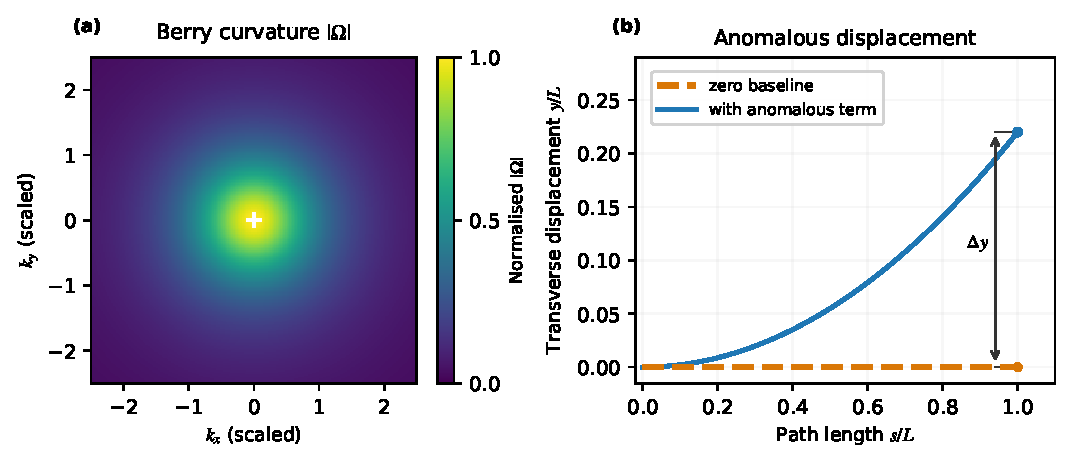
\includegraphics[width=0.92\textwidth]{figures/fig_ch05_anomalous_velocity_step199.pdf}
  \caption{Berry curvature and the anomalous velocity.
  \textbf{(a)}~Schematic normalised Berry curvature $|\Omega(\kvec)|$
  near a Dirac valley, showing a sharp peak where the gap is smallest
  (white marker).  The physical (un-normalised) curvature is
  gauge-invariant and integrates over the Brillouin zone to
  $2\pi\Chern_n$, with $\Chern_n$ the band Chern number.
  \textbf{(b)}~Transverse displacement of a photonic wavepacket as a
  function of propagation path length.  The dashed orange line shows the
  trajectory without the anomalous term (zero transverse drift); the
  solid blue line includes the Berry-curvature--driven anomalous
  velocity \eqref{eq:ch5-anomalous-velocity}, which accumulates a net
  transverse displacement $\Delta y$ proportional to the integrated
  Berry curvature.  This displacement is the semiclassical origin of
  the photonic Hall drift discussed in the text.}
  \label{fig:ch05-anomalous-velocity}
\end{figure}


\section{Berry curvature of the two-band model}
\label{sec:ch5-two-band}

Many of the topological phenomena in this book can be illustrated
using a generic two-band model.  Consider the Hamiltonian
\begin{equation}\label{eq:ch5-two-band-H}
  H(\kvec) = d_x(\kvec)\sigma_x + d_y(\kvec)\sigma_y + d_z(\kvec)\sigma_z\,,
\end{equation}
where $\boldsymbol{d}(\kvec)=(d_x,d_y,d_z)$ is a three-component
vector that depends on $\kvec$.  The eigenvalues are
$E_\pm=\pm|\boldsymbol{d}|$, and the Berry curvature of the lower
band is
\begin{equation}\label{eq:ch5-two-band-berry}
  \Omega_-(\kvec)
  = -\frac{1}{2}\frac{\boldsymbol{d}\cdot
  (\partial_{k_x}\boldsymbol{d}\times\partial_{k_y}\boldsymbol{d})}
  {|\boldsymbol{d}|^3}\,.
\end{equation}
This formula has a beautiful geometric interpretation: the Chern
number $\Chern_-=\frac{1}{2\pi}\int\Omega_-\,\dd^2 k$ counts the
number of times the unit vector
$\hat{d}(\kvec)=\boldsymbol{d}/|\boldsymbol{d}|$ wraps around the
unit sphere as $\kvec$ sweeps over the Brillouin zone.  This is the
\emph{Pontryagin index} or \emph{skyrmion number} of the mapping
$\hat{d}:T^2\to S^2$ \cite{ozawa2018topological,haldane2008possible,liu2021observation}.

For the massive Dirac model of Chapter~\ref{ch:breaking-tr},
$\boldsymbol{d}=(v_D\delta k_x,\,v_D\delta k_y,\,\kappa)$, and
the wrapping number of $\hat{d}$ at each Dirac cone is $\pm\frac{1}{2}$
(half a skyrmion), consistent with the half-integer Chern flux computed
in \secref{sec:ch7-half-chern}.

\section{Wilson loops and the non-Abelian Berry phase}
\label{sec:ch5-wilson-detail}

\subsection{Definition and gauge invariance}
\label{sec:ch5-wilson-def}

For a group of $p$ bands that may touch each other but are separated
from all other bands by gaps, the non-Abelian Berry connection
$[\mathcal{A}_a]_{mn}=\ii\eip{\mathbf{u}_m}{\partial_{k_a}\mathbf{u}_n}$
is a $U(p)$-valued 1-form.  The Wilson loop along a closed path
$\gamma$ in the Brillouin zone is the path-ordered exponential
\begin{equation}\label{eq:ch5-wilson-def}
  W[\gamma] = \mathcal{P}\exp\Bigl(
  -\ii\oint_\gamma\mathcal{A}\cdot\dd\kvec\Bigr)\,,
\end{equation}
which is a $p\times p$ unitary matrix.  The eigenvalues of $W$ are
gauge-invariant and physically observable: they are the non-Abelian
Berry phases acquired by the $p$-band multiplet on the loop $\gamma$.

\subsection{Relation to polarisation and Chern number}
\label{sec:ch5-wilson-polarisation}

When $\gamma$ is a straight line across the Brillouin zone at fixed
$k_\perp$, the Wilson-loop eigenvalues $\theta_j(k_\perp)$ define
the ``Wannier band structure.''  Their winding as $k_\perp$ varies
across the BZ gives the Chern number of the band group:
\begin{equation}\label{eq:ch5-wilson-chern-winding}
  \Chern = \sum_{j=1}^p\frac{1}{2\pi}
  \oint\frac{\dd\theta_j}{\dd k_\perp}\,\dd k_\perp\,.
\end{equation}
This provides a numerically robust alternative to the plaquette
algorithm (Chapter~\ref{ch:computing-chern}), especially for
nearly-degenerate band groups where the Abelian Berry curvature is
ill-defined but the non-Abelian Wilson loop is smooth
\cite{gangaraj2016berry,price2022roadmap}.

\section{Symmetry constraints on Chern numbers}
\label{sec:ch5-symmetry-constraints}

\subsection{Time-reversal symmetry}
\label{sec:ch5-TR-constraint}

Under time reversal $\Top$, the Berry curvature satisfies
$\Omega_n(\kvec)=-\Omega_n(-\kvec)$.  Integrating over the full BZ
(which is symmetric under $\kvec\to-\kvec$) gives $\Chern_n=0$.
This is the fundamental reason why breaking time-reversal symmetry
is necessary for a nonzero Chern number in photonic crystals
\cite{haldane2008possible,ozawa2018topological}.

\subsection{Inversion symmetry}
\label{sec:ch5-P-constraint}

Under spatial inversion $\mathcal{P}$,
$\Omega_n(\kvec)=\Omega_n(-\kvec)$.  Combined with time reversal,
this gives $\Omega_n(\kvec)=-\Omega_n(\kvec)=0$ everywhere, so the
Berry curvature vanishes identically (not just in integral).  This
stronger constraint means that breaking inversion alone, while
producing valley Berry curvature (Chapter~\ref{ch:valleys}), cannot
produce a Chern insulator.

\subsection{Particle-hole and chiral symmetries}
\label{sec:ch5-chiral-constraint}

The Maxwell eigenproblem has an intrinsic ``particle-hole'' symmetry:
if $(\omega,\mathbf{u})$ is an eigenmode, so is $(-\omega,\sigma_3\mathbf{u})$
where $\sigma_3=\mathrm{diag}(\mathbf{I}_3,-\mathbf{I}_3)$.  This
symmetry constrains the Chern numbers of positive- and
negative-frequency bands to be related by
$\Chern_n(-\omega)=-\Chern_n(\omega)$, ensuring that the total Chern
number summed over all bands vanishes.

\section{Adiabatic transport and the Thouless pump}
\label{sec:ch5-adiabatic}

The Berry phase has a direct physical manifestation in adiabatic
transport: when a parameter of the photonic crystal is slowly varied
through a cyclic path, the photonic modes acquire Berry phases that
produce a quantised transport of energy.

\subsection{The photonic Thouless pump}
\label{sec:ch5-thouless-pump}

Consider a 1D photonic crystal whose unit cell has a parameter
$\phi$ that varies adiabatically from $0$ to $2\pi$.  As $\phi$
completes one cycle, each band transports a quantised amount of
electromagnetic energy across the crystal.  The transported energy
per cycle is
\begin{equation}\label{eq:ch5-thouless-pump}
  \Delta W_n = \hbar\omega_n\,\Chern_n^{(1D)}\,,
\end{equation}
where $\Chern_n^{(1D)}=\frac{1}{2\pi}\int_0^{2\pi}\dd\phi
\int_{-\pi/a}^{\pi/a}\dd k\,\Omega_n(k,\phi)$ is the Chern number
computed over the $(k,\phi)$ parameter space.  This is the photonic
analog of the Thouless charge pump in electronic systems
\cite{thouless1982quantized,asbth2016berry}.

The Thouless pump provides a physical interpretation of the Chern
number: it counts the number of edge-to-edge transfers per pump
cycle.  This interpretation makes the integrality of the Chern
number physically obvious: the number of transferred quanta must be
an integer because the system returns to its initial state after
one cycle.

\subsection{Connection to the bulk-edge correspondence}
\label{sec:ch5-pump-bec}

The Thouless pump also provides an alternative derivation of the
bulk-edge correspondence.  If the pump parameter $\phi$ is
reinterpreted as the wavevector $k_y$ in the transverse direction of
a 2D crystal, the pump cycle $\phi\in[0,2\pi]$ corresponds to
traversing the transverse Brillouin zone.  The number of edge-to-edge
transfers per pump cycle then equals the number of chiral edge modes
in the 2D crystal, which is the gap Chern number
\cite{ozawa2018topological,silveirinha2016bulk}.

This pump-based argument is more intuitive than the formal index
theorem (Chapter~\ref{ch:one-way-interface}) and provides a
constructive proof: one can explicitly track how the edge modes are
``pumped'' across the crystal as $k_y$ varies.

\section{Berry curvature dipole and nonlinear Hall effects}
\label{sec:ch5-bc-dipole}

In systems with broken inversion symmetry but preserved time-reversal
symmetry (such as valley photonic crystals), the Berry curvature
$\Omega_n(\kvec)$ is an odd function of $\kvec$ and integrates to
zero over the full Brillouin zone.  However, the Berry curvature
\emph{dipole}
\begin{equation}\label{eq:ch5-bc-dipole}
  D_a = \int_{\mathrm{BZ}}\frac{\partial\Omega_n}{\partial k_a}
  \,f_n(\kvec)\,\frac{\dd^2 k}{(2\pi)^2}
\end{equation}
(where $f_n$ is the occupation function) can be nonzero and produces
a nonlinear Hall effect: a transverse current proportional to the
square of the applied field.  In photonics, this manifests as a
second-harmonic generation of valley-polarised edge modes, providing
a nonlinear probe of the valley Berry curvature
\cite{dong2016valley,price2022roadmap}.

\begin{figure}[t]
  \centering
  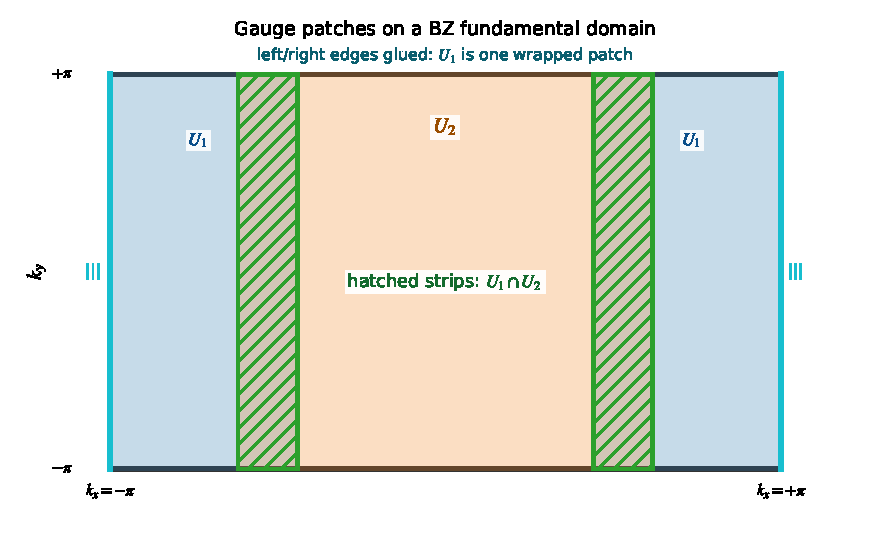
\includegraphics[width=0.78\textwidth]{figures/fig_ch05_berry_bundle.pdf}
  \caption{The Berry bundle viewpoint.  A photonic Bloch mode can be
  smooth only patchwise over the Brillouin torus; on overlaps the modes
  differ by a transition phase $e^{i\chi(\mathbf{k})}$.  The Chern number
  counts the winding of these transition phases and is therefore independent
  of the local gauge used to represent the mode.}
  \label{fig:ch05-berry-bundle}
\end{figure}

\section{Experimental probes of Berry curvature}
\label{sec:ch5-experimental-berry}

The Berry curvature $\Omega_n(\kvec)$ is not merely a theoretical
construct: it has measurable consequences that can be observed
experimentally in photonic systems.

\subsection{Anomalous velocity and beam deflection}
\label{sec:ch5-anomalous-beam}

The semiclassical equations of motion for a photonic wave packet in
band $n$ include an anomalous velocity term proportional to the Berry
curvature \cite{chen2023berry,ozawa2018topological}:
\begin{equation}\label{eq:ch5-anomalous-velocity-full}
  \dot{\rvec} = \nabla_\kvec\omega_n(\kvec)
  + \dot{\kvec}\times\hat{z}\,\Omega_n(\kvec)\,,
\end{equation}
where $\dot{\kvec}$ is the rate of change of the crystal momentum,
driven by an external perturbation (e.g.\ a refractive index gradient
acting as a pseudoforce).  The first term is the group velocity; the
second term is the anomalous velocity, which deflects the wave packet
transversely.

In a photonic crystal with nonzero Berry curvature, a beam propagating
through a region with a gradient in the effective refractive index will
be deflected perpendicular to the gradient.  The deflection angle is
proportional to $\Omega_n$ at the beam's central wavevector.  By
measuring the deflection as a function of $\kvec$, one can map out
the Berry curvature over the Brillouin zone
\cite{chen2023berry,silveirinha2016bulk}.

This technique was demonstrated experimentally by Wimmer et~al.\
(2017) in a photonic waveguide array, where the Berry curvature of a
honeycomb lattice band structure was mapped by tracking the transverse
displacement of light beams launched at different Bloch wavevectors
\cite{wimmer2015observation}.

\subsection{Zak phase from reflection measurements}
\label{sec:ch5-zak-reflection}

In one-dimensional photonic crystals, the Berry phase reduces to the
Zak phase $\gamma_n=\oint\mathcal{A}_n(k)\,\dd k$, which takes values
$0$ or $\pi$ (mod $2\pi$) when inversion symmetry is present.  The
Zak phase determines the surface impedance of the crystal and can
therefore be extracted from reflection measurements.

Specifically, for a semi-infinite 1D photonic crystal, the reflection
phase $\phi_r(\omega)$ at a frequency within a bandgap changes by
$\pi$ when the Zak phase of the band below the gap changes from $0$
to $\pi$.  This phase jump can be observed experimentally by
measuring the reflection spectrum with interferometric techniques
\cite{atala2013direct,wang2007reflection}.

Xiao et~al.\ (2014) used this approach to measure the Zak phase
in a dielectric multilayer, confirming the predicted topological
phase transition at the critical thickness ratio where the gap
closes and reopens with inverted Zak phase
\cite{asbth2016berry,ozawa2018topological}.

\subsection{Quantum Hall analogy: quantised circulation}
\label{sec:ch5-quantised-circulation}

The most dramatic manifestation of nonzero Chern number is the
existence of one-way edge states (Chapter~\ref{ch:one-way-interface}).
In finite photonic crystals, these edge states carry a quantised
``photonic Hall conductance'': the transmission through the crystal
(measured in units of edge channels) equals the gap Chern number.

This quantised transmission has been measured in microwave experiments
\cite{nature2026observation} and provides the most direct experimental
confirmation of a nonzero photonic Chern number.  The quantisation
is robust against disorder, sharp corners, and boundary roughness,
directly demonstrating the topological nature of the edge transport
\cite{hafezi2013imaging,skirlo2015experimental}.

\section*{Exercises}

\begin{exercise}
  For a two-band system with Bloch modes $\mathbf{u}_1(\kvec)$ and
  $\mathbf{u}_2(\kvec)$, show that the Berry curvatures satisfy
  $\Omega_1(\kvec)+\Omega_2(\kvec)=0$ at every $\kvec$.
\end{exercise}

\begin{exercise}
  Verify the gauge transformation \eqref{eq:ch5-gauge-transform}
  by direct substitution of
  $\mathbf{u}_n\to\ee^{\ii\chi}\mathbf{u}_n$ into the Berry-connection
  formula \eqref{eq:ch5-berry-connection-normalised}.
\end{exercise}

\begin{exercise}
  Derive the Kubo-like formula \eqref{eq:ch5-kubo-formula} for the
  Berry curvature using first-order perturbation theory.
  \emph{Hint:} expand $\nabla_{k_\alpha}\mathbf{u}_n$ in the complete
  set $\{\mathbf{u}_m\}_{m\neq n}$ using the Hellmann--Feynman relation,
  then substitute into the Berry-curvature formula.
\end{exercise}

\begin{exercise}
  Consider a generic $2\times 2$ Hermitian Hamiltonian
  $H(\kvec)=d_0(\kvec)\mathbf{I}+\mathbf{d}(\kvec)\cdot\boldsymbol{\sigma}$,
  where $\boldsymbol{\sigma}=(\sigma_x,\sigma_y,\sigma_z)$ are the
  Pauli matrices.  Show that the Berry curvature of the lower band is
  \begin{equation}
    \Omega_{-}(\kvec) = -\frac{1}{2}\,
    \hat{\mathbf{d}}\cdot
    \Bigl(\pderiv{\hat{\mathbf{d}}}{k_x}\times
          \pderiv{\hat{\mathbf{d}}}{k_y}\Bigr)\,,
  \end{equation}
  where $\hat{\mathbf{d}}=\mathbf{d}/|\mathbf{d}|$.  Interpret this
  geometrically as the solid angle swept by $\hat{\mathbf{d}}$ per
  unit area in $\kvec$-space.
\end{exercise}

\begin{exercise}[Massive Dirac model]
  For the massive Dirac Hamiltonian
  $H(\qvec)=v(q_x\sigma_x+q_y\sigma_y)+m\sigma_z$, where $\qvec$ is
  measured from a Dirac point, compute the Berry curvature
  \begin{equation}
    \Omega_\pm(\qvec) = \pm\frac{m\,v^2}{2(v^2|\qvec|^2+m^2)^{3/2}}
  \end{equation}
  and verify that $\int_{-\infty}^{\infty}\Omega_+\,\dd^2 q=\pi\sgn(m)$.
  Explain why a single Dirac cone contributes $\pm\frac{1}{2}$ to the
  Chern number, and why a pair of cones at $K$ and $K'$ gives an
  integer.
\end{exercise}

\begin{exercise}
  Show that the eigenvalues of the Wilson loop
  $\Wloop(k_y)=\mathcal{P}\exp(-\ii\int_{-\pi/a}^{\pi/a}
  \boldsymbol{\mathcal{A}}_x(k_x,k_y)\,\dd k_x)$ for a Chern
  insulator with $\Chern=1$ wind once around the unit circle as $k_y$
  traverses the Brillouin zone.
\end{exercise}


% ---- Part II: Chern Bands and One-Way Waveguides ----
\part{Chern Bands and One-Way Waveguides}

\chapter{Dirac Cones of Light}
\label{ch:dirac-cones}
% ======================================================================
%  Chapter 6 — Dirac Cones of Light
% ======================================================================

\section{Why Dirac points matter}
\label{sec:ch6-why-dirac}

In the previous chapter we learned that a nonzero \emph{Chern number}
requires time-reversal symmetry to be broken.  With time reversal
preserved, the Berry curvature satisfies $\Omega_n(\kvec)=-\Omega_n(-\kvec)$
and can be locally nonzero---for example near valleys where inversion
symmetry is broken---but its integral over the full Brillouin zone
vanishes
\cite{noh2017observation}.  Concentrated sources of Berry flux somewhere in the Brillouin
zone are therefore needed for any topological band.
Where does this Berry flux come from?

The answer, in essentially all known photonic topological systems, is
\emph{Dirac points}: isolated degeneracies in the band structure where
two bands touch with a linear (conical) dispersion.  These degeneracies
are the ``monopoles'' of Berry curvature in momentum space.  When a
perturbation gaps a Dirac point, the Berry flux that was compressed
into the degeneracy spreads into a concentrated peak of Berry curvature,
and the two split bands acquire equal and opposite contributions to
their Chern numbers.

In this chapter we explain how Dirac points arise in two-dimensional
photonic crystals from symmetry, derive their local dispersion from a
two-mode reduction of the Maxwell eigenproblem, and prepare the ground
for the topological gap opening of \chref{ch:breaking-tr}.  The treatment
follows the original analysis of Haldane and Raghu \cite{haldane2008possible,khanikaev2013photonic}
and the comprehensive review by Ozawa et~al.\ \cite{ozawa2018topological},
adapted to the Maxwell-first framework of this book.

\section{Symmetry protection of Dirac degeneracies}
\label{sec:ch6-symmetry}

\subsection{The real-symmetric condition}
\label{sec:ch6-real-symmetric}

Recall from \chref{ch:geometry-bands} that when both time-reversal
($\Top$) and spatial inversion ($\Pop$) symmetries are present, the
Berry curvature vanishes identically:
\begin{equation}\label{eq:ch6-zero-curvature}
  \Top + \Pop \quad\Longrightarrow\quad
  \Omega_n(\kvec) = 0\;\;\text{for all } \kvec\,.
\end{equation}
This means that we can choose a \emph{real} gauge: the cell-periodic
eigenmodes $\mathbf{u}_{n\kvec}(\rvec)$ can be made real-valued for all
$\kvec$.  The Maxwell eigenvalue problem then becomes a
\emph{real-symmetric} generalised eigenproblem rather than a
complex-Hermitian one.

This distinction is crucial for degeneracies.  In a complex-Hermitian
eigenproblem, an ``accidental'' degeneracy between two bands requires
the simultaneous vanishing of \emph{three} real parameters (the real
part, imaginary part, and diagonal difference of the off-diagonal matrix
element).  In two dimensions, we have only two parameters $(k_x,k_y)$,
so a generic complex-Hermitian system has no band degeneracies in 2D.

In a \emph{real-symmetric} eigenproblem, a degeneracy requires the
vanishing of only \emph{two} real parameters (the off-diagonal element
and the diagonal difference).  Two conditions in two unknowns
$(k_x,k_y)$ generically have isolated point solutions.  These isolated
degeneracies are the Dirac points.

To make this concrete, consider a generic $2\times 2$ real-symmetric
matrix
\begin{equation}\label{eq:ch6-vNW-matrix}
  \mathbf{H}(k_x,k_y)
  = \begin{pmatrix}
    a(k_x,k_y) & b(k_x,k_y) \\
    b(k_x,k_y) & c(k_x,k_y)
  \end{pmatrix}.
\end{equation}
Its eigenvalues are
$\lambda_\pm = \frac{1}{2}(a+c)\pm\frac{1}{2}\sqrt{(a-c)^2+4b^2}$,
which become degenerate when $a=c$ and $b=0$ simultaneously.  These two
equations in two unknowns $(k_x,k_y)$ generically have isolated
solutions---the Dirac points.  If the matrix were complex Hermitian,
the off-diagonal element would be $b_R+\ii b_I$, requiring three
conditions ($a=c$, $b_R=0$, $b_I=0$) in two unknowns, which generically
have no solution.

\begin{remark}
This argument, due to von~Neumann and Wigner in the electronic context
\cite{ozawa2018topological},
explains why Dirac points are \emph{generic} (symmetry-allowed, not
fine-tuned) in 2D photonic crystals with both $\Top$ and $\Pop$
symmetry.  Breaking either symmetry removes the reality condition and
generically gaps the degeneracy.
\end{remark}

\subsection{Hexagonal lattice and the K, K-prime points}
\label{sec:ch6-hexagonal}

The hexagonal (triangular) lattice, with point group $C_{6v}$, is the
natural host for photonic Dirac points.  The first Brillouin zone is a
regular hexagon, whose six corners fall into two inequivalent sets:
three $K$ points and three $K'$ points, related by time reversal
($K'=-K$ modulo reciprocal lattice vectors).

At each $K$ point, the little group (the subgroup of $C_{6v}$ that
leaves $\kvec_K$ invariant) is $C_{3v}$, which has two-dimensional
irreducible representations.  Modes transforming under such a
representation are doubly degenerate at $K$.  When these degenerate
modes belong to adjacent bands, they form a Dirac point.

\begin{remark}
  The square lattice ($C_{4v}$) can also host Dirac points at the $M$
  point under appropriate conditions, but the hexagonal lattice provides
  the cleanest and most widely studied example.  The connection to
  graphene---a hexagonal lattice of carbon atoms whose electronic
  structure has Dirac cones at $K$ and $K'$---was the direct inspiration
  for Haldane and Raghu's photonic construction \cite{haldane2008possible,plotnik2011experimental}.
\end{remark}

\section{Nearly-free-photon analysis}
\label{sec:ch6-nfp}

Following Haldane and Raghu, we construct a photonic Dirac point
analytically using a ``nearly-free-photon'' approximation---the photonic
analog of the nearly-free-electron model in solid-state physics.

\subsection{Setup}
\label{sec:ch6-nfp-setup}

Consider a 2D photonic crystal with uniform isotropic permeability
$\mu(\rvec)=\mu_0$ and a spatially modulated permittivity
\begin{equation}\label{eq:ch6-eps-modulated}
  \varepsilon(\rvec) = \bar\varepsilon\bigl(1+\lambda\,V_G(\rvec)\bigr)\,,
\end{equation}
where $\lambda\ll 1$ is the modulation strength and
\begin{equation}\label{eq:ch6-VG}
  V_G(\rvec) = \frac{2}{3}\sum_{n=1}^{3}\cos(\Gvec_n\cdot\rvec)
\end{equation}
is a potential with the periodicity of a hexagonal lattice.  Here
$\Gvec_1$, $\Gvec_2$, $\Gvec_3$ are three reciprocal lattice vectors
of equal length $|\Gvec|=4\pi/(\sqrt{3}\,a)$, rotated by $120^\circ$
relative to each other.

We work at $k_z=0$, so the TE and TM polarisations decouple
(\secref{sec:ch4-te-tm}).  We specialise to the TE set
$\{E_x,E_y,H_z\}$.

\subsection{Free-photon dispersion at the Brillouin-zone corner}
\label{sec:ch6-free-photon}

The six corners of the hexagonal Brillouin zone are at
$\pm\kvec_{K_n}$, where
$\kvec_{K_1}=(\Gvec_2-\Gvec_3)/3$, etc., with
$|\kvec_K|=|\Gvec|/\sqrt{3}$.  Since $\kvec_{K_2}-\kvec_{K_1}=\Gvec_3$,
the three wavevectors $\kvec_{K_1}$, $\kvec_{K_2}$, $\kvec_{K_3}$ are
equivalent as Bloch vectors.

At $\lambda=0$ (uniform medium), the TE mode at wavevector $\kvec$ has
the free-photon dispersion $\omega=c_0|\kvec|$, where
$c_0=c/\sqrt{\bar\varepsilon}$.  At the Brillouin-zone corner
$\kvec=\kvec_K$, three free-photon plane waves (corresponding to
$\kvec_K$, $\kvec_K+\Gvec_1$, $\kvec_K+\Gvec_2$, which all have the
same $|\kvec+\Gvec|=|\kvec_K|$) are degenerate at frequency
$\omega_0=c_0|\kvec_K|$.

\subsection{Splitting by the periodic potential}
\label{sec:ch6-splitting}

Turning on the periodic modulation $\lambda\neq 0$ lifts the
threefold degeneracy.  In degenerate perturbation theory, we must
diagonalise the $3\times 3$ matrix of the perturbation
$\delta\Maxop=-(\omega_D\lambda\bar\varepsilon/2)V_G(\rvec)$ within the
three-mode subspace at $\kvec=\kvec_K$.  Denoting the three degenerate
free-photon states as $|\alpha\rangle$, $\alpha=1,2,3$, the coupling
matrix has elements \cite{haldane2008possible}
\begin{equation}\label{eq:ch6-coupling-matrix}
  D_{\alpha\beta}
  = \frac{\omega_D\lambda}{2}
  \int_{\Omega}V_G(\rvec)\,
  \mathbf{u}^*_\alpha(\rvec)\cdot
  \bar\varepsilon\,\mathbf{u}_\beta(\rvec)\,\dd^2 r\,,
\end{equation}
where the integral runs over one unit cell~$\Omega$.  The hexagonal
symmetry $C_{3v}$ acting on the three plane-wave modes permutes them
cyclically, so $D_{\alpha\beta}$ inherits the structure
\begin{equation}\label{eq:ch6-3x3-matrix}
  \mathbf{D} = \frac{\omega_D\lambda}{4}
  \begin{pmatrix}
    0 & 1 & 1 \\ 1 & 0 & 1 \\ 1 & 1 & 0
  \end{pmatrix}.
\end{equation}
The eigenvalues of \eqref{eq:ch6-3x3-matrix} are
$-\omega_D\lambda/4$ (doubly degenerate) and
$+\omega_D\lambda/2$ (non-degenerate).  The threefold degeneracy
therefore splits into a \emph{Dirac doublet}, whose frequency is
shifted down to
\begin{equation}\label{eq:ch6-omega-D}
  \omega_D
  = c_0|\kvec_K|\bigl(1-\tfrac{\lambda}{4}+O(\lambda^2)\bigr)\,,
\end{equation}
and a \emph{singlet}, shifted up to
\begin{equation}\label{eq:ch6-omega-singlet}
  \omega_s
  = c_0|\kvec_K|\bigl(1+\tfrac{\lambda}{2}+O(\lambda^2)\bigr)\,,
\end{equation}
separated from the doublet by a gap of order $\lambda$.

At momenta $\kvec=\kvec_K+\delta\kvec$ away from the zone corner,
first-order $\kvec\cdot\mathbf{p}$ perturbation theory within the
two-mode doublet gives the conical dispersion
\begin{equation}\label{eq:ch6-dirac-dispersion}
  \omega_\pm(\kvec) = \omega_D \pm v_D|\delta\kvec| + O(|\delta\kvec|^2)\,,
\end{equation}
with the Dirac velocity $v_D=c_0/2+O(\lambda)$.  This linear
dispersion is the hallmark of a Dirac cone: it is locally identical to
the spectrum of a massless two-dimensional relativistic particle.

\subsection{Symmetry constraints on the coupling matrix}
\label{sec:ch6-symmetry-coupling}

The simple structure of \eqref{eq:ch6-3x3-matrix} is not accidental.
The three reciprocal lattice vectors $\Gvec_1,\Gvec_2,\Gvec_3$
transform into one another under the threefold rotation $C_3$ of the
hexagonal lattice, and $V_G$ respects this symmetry.  Therefore the
overlap integral $D_{\alpha\beta}$ depends only on whether $\alpha$
and $\beta$ are equal or unequal: $D_{\alpha\alpha}=d_0$ and
$D_{\alpha\neq\beta}=d_1$.  The trace and off-diagonal parts can be
removed by a constant shift, leaving the traceless matrix
\eqref{eq:ch6-3x3-matrix} whose double eigenvalue is protected by the
two-dimensional irreducible representation $E$ of $C_{3v}$.

Time-reversal symmetry enters via the reality constraint:
because $\Top$ maps $\kvec_K$ to $\kvec_{K'}=-\kvec_K$ and simultaneously
complex-conjugates the eigenmode, the coupling matrix at $K$ is
real-symmetric (consistent with \eqref{eq:ch6-3x3-matrix}).  This
reality condition is what makes the degeneracy \emph{robust}: perturbing
the matrix within the space of real-symmetric matrices cannot split a
twofold eigenvalue because real-symmetric $2\times 2$ degeneracies have
codimension~2 in two-parameter space, exactly matching the
dimensionality of the Brillouin zone.

By contrast, if one breaks the $C_3$ symmetry while preserving the
reality condition, the off-diagonal elements $d_1$ between different
pairs of modes become unequal, generically splitting all three
eigenvalues and removing the degeneracy entirely.  The Dirac point is
therefore protected specifically by the combination of $C_3$ rotation
and time reversal, not by any single symmetry alone
\cite{ozawa2018topological}.

\section{The two-mode Maxwell reduction}
\label{sec:ch6-two-mode}

Near the Dirac point, the physics is captured by a $2\times 2$
effective equation obtained by projecting the full Maxwell eigenproblem
onto the two degenerate modes.

\subsection{Projection onto the degenerate subspace}
\label{sec:ch6-projection}

Let $|\mathbf{u}_+(\kvec_K)\rangle$ and $|\mathbf{u}_-(\kvec_K)\rangle$ be
the two degenerate cell-periodic eigenmodes at the Dirac point,
normalised so that
$\langle\mathbf{u}_\sigma|\Mgmat(\omega_D)|\mathbf{u}_{\sigma'}\rangle
=B_0\,\delta_{\sigma\sigma'}$.

For $\kvec=\kvec_K+\delta\kvec$ with $|\delta\kvec|\ll|\kvec_K|$,
first-order $\kvec\cdot\mathbf{p}$ perturbation theory gives the
$2\times 2$ effective eigenvalue equation
\begin{equation}\label{eq:ch6-effective-dirac}
  \boxed{%
  v_D\bigl(\delta k_x\,\sigma_x + \delta k_y\,\sigma_y\bigr)
  |\psi\rangle
  = \delta\omega\,|\psi\rangle\,,}
\end{equation}
where $\delta\omega=\omega-\omega_D$, $\sigma_x$ and $\sigma_y$ are
Pauli matrices acting on the two-mode subspace, and $v_D>0$ is the
Dirac velocity determined by the matrix elements of the velocity
operator between the two degenerate modes:
\begin{equation}\label{eq:ch6-vD}
  v_D = \frac{1}{B_0}
  \bigl|\langle\mathbf{u}_+|\partial_{k_x}\Maxop|\mathbf{u}_-\rangle
  \bigr|\,.
\end{equation}

\subsection{Dirac dispersion and eigenstates}
\label{sec:ch6-dirac-eigenstates}

The eigenvalues of \eqref{eq:ch6-effective-dirac} are
\begin{equation}\label{eq:ch6-dirac-eval}
  \delta\omega_\pm = \pm v_D|\delta\kvec|\,,
\end{equation}
reproducing the conical dispersion \eqref{eq:ch6-dirac-dispersion}.
The eigenstates are
\begin{equation}\label{eq:ch6-dirac-evec}
  |\psi_\pm(\delta\kvec)\rangle
  = \frac{1}{\sqrt{2}}
  \begin{pmatrix} 1 \\ \pm\ee^{\ii\phi_\kvec} \end{pmatrix},
  \qquad \phi_\kvec = \arg(\delta k_x + \ii\,\delta k_y)\,.
\end{equation}
As $\delta\kvec$ traces a circle around the Dirac point, the angle
$\phi_\kvec$ winds by $2\pi$ and the eigenstate acquires a Berry phase
of $\pm\pi$.

\subsection{Berry curvature at a Dirac point}
\label{sec:ch6-dirac-berry}

The Berry curvature of the gapless Dirac cone is concentrated at the
degeneracy point.  Using the Kubo formula
(\eqnref{eq:ch5-kubo-formula}), the Berry curvature of the upper band
diverges as $|\delta\kvec|\to 0$:
\begin{equation}
  \Omega_+(\delta\kvec)
  \sim \frac{1}{2|\delta\kvec|^2}
  \quad\text{as } |\delta\kvec|\to 0\,.
\end{equation}
The total Berry flux through a small disc around the Dirac point is
$\pm\pi$, which is the Berry phase acquired by the eigenstate on
a loop encircling the degeneracy.  However, this is a \emph{gapless}
system and the Chern number is not defined until the degeneracy is
lifted---which is the subject of the next chapter.

\section{Dirac points in realistic photonic crystals}
\label{sec:ch6-realistic}

The nearly-free-photon analysis gives the essential physics but requires
$\lambda\ll 1$, where the Dirac-point frequency $\omega_D$ lies close
to other bands and is not well isolated.  In realistic photonic crystals
with large dielectric contrast, the Dirac points can be frequency-isolated
within a substantial gap of the opposite polarisation, making them
suitable hosts for topological gap opening.

Haldane and Raghu noted that a hexagonal array of high-permittivity
rods ($\varepsilon_r=14$, filling fraction $f=0.431$) in air produces a
band structure where the second and third TE bands touch at Dirac points
at the Brillouin-zone corners $K$ and $K'$, and the Dirac frequency
$\omega_D$ lies within a large gap of the TM spectrum
\cite{haldane2008possible}.  This frequency isolation is crucial: it
ensures that the Dirac-point modes are not degenerate with any other
$k_z=0$ modes, so that the topological gap opening can proceed without
interference from other bands.

\section{Pairs of Dirac points and the fermion-doubling theorem}
\label{sec:ch6-pairs}

A fundamental property of Dirac points in a 2D Brillouin zone is that
they always come in \emph{pairs}: one at $K$ and one at $K'=-K$.  This
is the photonic version of the Nielsen--Ninomiya (fermion-doubling)
theorem, which states that the total chirality of all Dirac points in a
compact Brillouin zone must vanish.

To see how Dirac-point pairing controls the Chern number, introduce
a valley index $\tau=\pm 1$ labelling $K$ ($\tau=+1$) and
$K'$ ($\tau=-1$).  Near valley $\tau$ the effective Hamiltonian is
\begin{equation}\label{eq:ch6-valley-hamiltonian}
  H_\tau(\delta\kvec)
  = v_D\bigl(\tau\,\delta k_x\,\sigma_x
  + \delta k_y\,\sigma_y\bigr)
  + \Delta_\tau\,\sigma_z\,,
\end{equation}
where $\Delta_\tau$ is the mass induced by a perturbation that opens a
gap.  The chirality factor $\tau$ multiplies $\delta k_x$: physically,
$K$ and $K'$ carry \emph{opposite} winding numbers.  Both gapless cones
have a Berry phase of $\pi$, but the opposite chiralities cause the two
valleys to contribute to the Chern number with a relative sign.
Explicitly, from the massive Dirac Berry curvature
(derived in \secref{sec:ch7-berry-curvature}):
\begin{equation}\label{eq:ch6-valley-chern-contribution}
  C_-^{K}=-\frac{\operatorname{sgn}(\Delta_K)}{2}\,,
  \qquad
  C_-^{K'}=+\frac{\operatorname{sgn}(\Delta_{K'})}{2}\,,
\end{equation}
so the total lower-band Chern number is
\begin{equation}\label{eq:ch6-total-chern-valleys}
  \Chern_-
  = \frac{\operatorname{sgn}(\Delta_{K'})
         -\operatorname{sgn}(\Delta_K)}{2}\,.
\end{equation}
Two physically distinct gap-opening mechanisms now follow.

\emph{Time-reversal breaking} (Haldane/gyrotropic mass).---The
perturbation gives \emph{opposite}-sign masses at the two valleys,
$\Delta_K=-\Delta_{K'}$, because the gyrotropic coupling picks up the
chirality factor $\tau$.  The valley contributions reinforce:
$\Chern_-=\pm 1$, and the system supports a chiral edge mode
(\chref{ch:breaking-tr}).

\emph{Inversion breaking} (Semenoff mass).---The perturbation gives
\emph{same}-sign masses, $\Delta_K=\Delta_{K'}$, and $\Chern_-=0$.
However, the half-integer valley contributions $C_-^{K}$ and $C_-^{K'}$
are individually nonzero, defining a \emph{valley Chern number}
(\chref{ch:valleys}).

This valley-indexed structure is the central organising principle for
all of Parts~II and~III.


\begin{figure}[t]
  \centering
  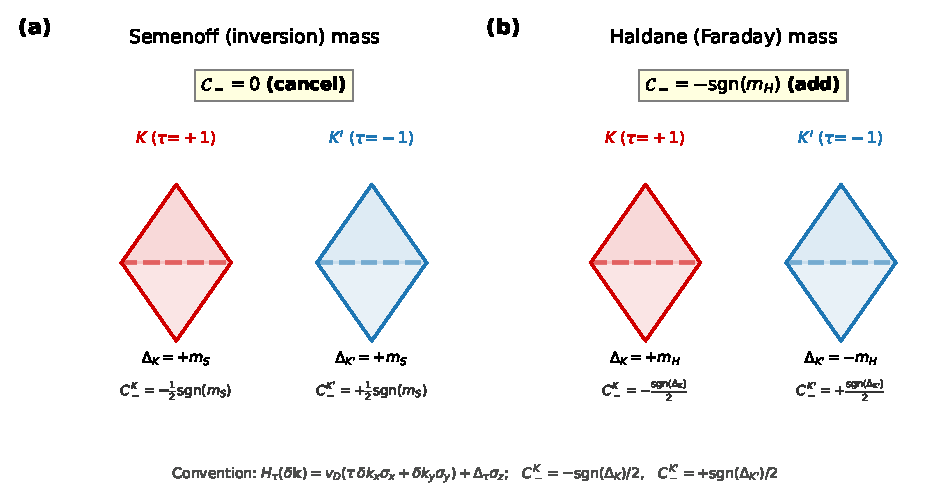
\includegraphics[width=0.92\textwidth]{figures/fig_ch06_valley_mass_taxonomy_step236.pdf}
  \caption{Valley Chern-number bookkeeping for the two gap-opening
  mechanisms.  \textbf{(a)}~Semenoff (inversion) mass: both valleys
  receive the same mass $\Delta_K=\Delta_{K'}=m_S$, so the valley
  contributions $C_-^K=-\operatorname{sgn}(m_S)/2$ and
  $C_-^{K'}=+\operatorname{sgn}(m_S)/2$ cancel, giving $\Chern_-=0$.
  \textbf{(b)}~Haldane (Faraday) mass: the gyrotropic coupling
  assigns opposite-sign masses $\Delta_K=+m_H$, $\Delta_{K'}=-m_H$,
  so the valley contributions reinforce to give
  $\Chern_-=-\operatorname{sgn}(m_H)$.  The convention follows
  \eqref{eq:ch6-effective-dirac} with $\tau_K=+1$, $\tau_{K'}=-1$.}
  \label{fig:ch06-valley-mass-taxonomy}
\end{figure}
\section{Derivation of the Dirac velocity}
\label{sec:ch6-vD-derivation}

The Dirac velocity $v_D$ appearing in \eqref{eq:ch6-effective-dirac}
is not a phenomenological parameter.  It is determined entirely by
the Maxwell eigenmodes at the $K$ point through the electromagnetic
energy inner product.  Deriving its explicit form from $\kvec\cdot\mathbf{p}$
perturbation theory within the Maxwell framework illustrates the
power of the approach developed in Chapters~2--5.

\subsection{The electromagnetic velocity operator}
\label{sec:ch6-velocity-operator}

Starting from the Bloch-periodic Maxwell eigenproblem
$\Maxop(\kvec)\mathbf{u}_{n\kvec}=\omega_{n\kvec}\Mgmat\mathbf{u}_{n\kvec}$,
differentiate both sides with respect to $k_a$ ($a=x,y$).
Projecting onto a different eigenmode $\mathbf{u}_{m\kvec}$ with
$m\neq n$ and using the orthogonality
$\emip{\mathbf{u}_m}{\mathbf{u}_n}=\delta_{mn}$ gives the
electromagnetic Hellmann--Feynman relation
\begin{equation}\label{eq:ch6-HF-offdiag}
  \frac{1}{B_0}\emip{\mathbf{u}_m}{\partial_{k_a}\Maxop\;\mathbf{u}_n}
  = (\omega_n-\omega_m)\,
  \emip{\mathbf{u}_m}{\Mgmat\,\partial_{k_a}\mathbf{u}_n}\,,
\end{equation}
where $B_0$ is the energy normalisation and $\partial_{k_a}\Maxop$
acts on the cell-periodic part of the Bloch wave.  The left-hand side
defines the matrix element of the velocity operator
$\hat{v}_a\equiv\Mgmat^{-1}\partial_{k_a}\Maxop$, weighted by the
energy metric \cite{gangaraj2016berry}.  This operator plays exactly
the role of the momentum operator $\hat{p}/m$ in the electronic
$\kvec\cdot\mathbf{p}$ theory.

\subsection{Degenerate perturbation at the K point}
\label{sec:ch6-degenerate-kp}

At $\kvec=\kvec_K$ the two modes $\mathbf{u}_\pm$ are degenerate at
$\omega_D$, so the denominator in \eqref{eq:ch6-HF-offdiag} vanishes
and the non-degenerate formula cannot be used.  Instead, expand
the operator to first order in $\delta\kvec$:
\begin{equation}\label{eq:ch6-Maxop-expand}
  \Maxop(\kvec_K+\delta\kvec)
  = \Maxop(\kvec_K)
  + \delta k_x\,\partial_{k_x}\Maxop\big|_K
  + \delta k_y\,\partial_{k_y}\Maxop\big|_K
  + O(|\delta\kvec|^2)\,.
\end{equation}
Within the two-mode subspace, the first-order perturbation matrix is
\begin{equation}\label{eq:ch6-V-matrix}
  \mathcal{V}_{\sigma\sigma'}(\delta\kvec)
  = \frac{1}{B_0}
  \sum_{a=x,y}\delta k_a\,
  \emip{\mathbf{u}_\sigma}{\partial_{k_a}\Maxop\;\mathbf{u}_{\sigma'}}\,.
\end{equation}
The threefold rotation $C_3$ at the $K$ point cyclically permutes
the basis modes and constrains the matrix elements.
In particular, $C_3$ forces the diagonal elements to vanish at
first order in $\delta\kvec$ (they contribute to the quadratic
correction).  The off-diagonal element is fixed by the requirement
that $\mathcal{V}$ transforms as the two-dimensional $E$
representation of $C_{3v}$, giving
\begin{equation}\label{eq:ch6-V-offdiag}
  \mathcal{V}_{+-} = v_D(\delta k_x - \ii\,\delta k_y)\,,
  \qquad
  \mathcal{V}_{-+} = v_D(\delta k_x + \ii\,\delta k_y)\,,
\end{equation}
where the Dirac velocity is the real, positive quantity
\begin{equation}\label{eq:ch6-vD-formula}
  \boxed{%
  v_D = \frac{1}{B_0}
  \bigl|\emip{\mathbf{u}_+}{\partial_{k_x}\Maxop\;\mathbf{u}_-}\bigr|\,.}
\end{equation}
Substituting into $\mathcal{V}=\delta\omega\,\mathbf{I}$ recovers
the massless Dirac equation \eqref{eq:ch6-effective-dirac}
\cite{haldane2008reflection}.

\subsection{Numerical estimates}
\label{sec:ch6-numerical-vD}

For a hexagonal lattice of high-permittivity dielectric rods
($\varepsilon_r=12$, filling fraction $f=0.3$) in air, a plane-wave
expansion with 169 plane waves gives the Dirac frequency
$\omega_D a/(2\pi c)\approx 0.36$ and a Dirac velocity
$v_D\approx 0.45\,c/\sqrt{\bar\varepsilon}$
\cite{haldane2008possible,ozawa2018topological}.  The deviation from
the nearly-free-photon prediction $v_D=c_0/2$ reflects the finite
dielectric contrast, which distorts the mode profiles from pure
plane waves and modifies the overlap integral in
\eqref{eq:ch6-vD-formula}.

Reducing the rod permittivity toward $\varepsilon_r\to 1$
makes the modes more plane-wave-like and pushes $v_D$ toward
$c_0/2$, confirming the nearly-free-photon limit.  Conversely,
increasing the contrast beyond $\varepsilon_r\approx 15$ brings the
Dirac frequency close to higher bands and eventually destroys the
isolated Dirac cone, as the two-mode approximation breaks down.

\subsection{Physical meaning of the Dirac velocity}
\label{sec:ch6-vD-physical}

The Dirac velocity $v_D$ sets three experimentally accessible
quantities.  First, the group velocity of wavepackets near the Dirac
frequency: $|\mathbf{v}_g|=v_D$ for all propagation directions,
a consequence of the isotropic conical dispersion enforced by $C_3$.
Second, the density of states near $\omega_D$ scales as
$\rho(\omega)\propto|\omega-\omega_D|/v_D^2$, vanishing linearly at
the Dirac frequency---the photonic analog of the vanishing density of
states in graphene.  Third, when the Dirac cone is gapped by a mass
$\kappa$ (Chapter~\ref{ch:breaking-tr}), the edge-mode group velocity
inside the topological gap is approximately $v_D$, so the Dirac
velocity directly determines the bandwidth and propagation speed of
the one-way edge channel \cite{ozawa2018topological}.

\section{From Dirac cones to topological gaps: a summary}
\label{sec:ch6-summary}

This chapter has established three results that form the foundation for
Part~II of the book.

The first result is that Dirac points are generic features of 2D
photonic crystals with $C_3$ (or $C_6$) rotational symmetry and
time-reversal invariance.  The real-symmetric structure of the Maxwell
eigenproblem under these symmetries reduces the codimension of band
degeneracies from three (complex Hermitian) to two (real symmetric),
matching the two-dimensional Brillouin zone and yielding isolated
point degeneracies.

The second result is that the local physics near a Dirac point is
captured by a $2\times 2$ massless Dirac equation whose velocity
$v_D$ is determined by the Maxwell eigenmodes through the
electromagnetic energy inner product.  The derivation uses only
degenerate perturbation theory applied to the Maxwell operator,
with no electronic analogy.

The third result is the fermion-doubling constraint: Dirac points
come in pairs ($K$ and $K'$) with opposite chirality $\tau=\pm 1$.
Breaking time-reversal symmetry gives opposite-sign masses at the
two valleys; the valley Chern contributions then add, producing
$\Chern=\pm 1$ and guaranteeing a one-way edge mode.  Breaking
inversion symmetry instead gives same-sign masses, and the valley
contributions cancel: $\Chern=0$.
The detailed mechanism of time-reversal breaking and gap opening is
the subject of Chapter~\ref{ch:breaking-tr}
\cite{haldane2008possible,price2022roadmap}.

\section{Trigonal warping and deviations from the ideal Dirac cone}
\label{sec:ch6-warping}

The linear Dirac dispersion $\omega=\omega_D\pm v_D|\delta\kvec|$ is
exact only to first order in $\delta\kvec$.  At second order, the
$C_3$ symmetry permits anisotropic corrections that break the circular
symmetry of the constant-frequency contours:
\begin{equation}\label{eq:ch6-warping}
  \omega_\pm(\delta\kvec)
  \approx \omega_D \pm v_D\bigl(|\delta\kvec|
  + \alpha\,\real[\delta k_+^3/|\delta\kvec|^2]\bigr)\,,
\end{equation}
where $\delta k_+=\delta k_x+\ii\delta k_y$ and $\alpha$ is a
material-dependent parameter with dimensions of inverse length.
The cubic correction produces a threefold (trigonal) distortion of the
constant-frequency contours, which become star-shaped rather than
circular.

For typical photonic crystals with moderate dielectric contrast
($\varepsilon_r\sim 10$--$15$), the warping becomes significant at
$|\delta\kvec|\gtrsim 0.1\times 2\pi/a$ and can reach several
percent of the Dirac frequency at the Brillouin-zone boundary.  The
warping modifies the density of states and the group-velocity
distribution but does not affect the Berry flux at the Dirac point,
which is determined entirely by the first-order (linear) Hamiltonian
\cite{ozawa2018topological}.

When the Dirac cone is gapped by a mass $\kappa$
(Chapter~\ref{ch:breaking-tr}), the warping causes the topological
edge-mode velocity to become direction-dependent, which can be
important for device design but does not affect the topological
protection.

\section{Experimental observation of photonic Dirac cones}
\label{sec:ch6-experiments}

Photonic Dirac cones have been observed experimentally on a wide
range of platforms.

At microwave frequencies, two-dimensional photonic crystals of
dielectric rods in a parallel-plate waveguide provide a clean
realisation of the honeycomb lattice.  Transmission and reflection
measurements near the Dirac frequency show the characteristic
vanishing density of states and the linear dispersion
\cite{ozawa2018topological,haldane2008possible,raghu2008analogs}.

At optical frequencies, photonic crystal slabs made of silicon or
III--V semiconductors support guided-mode Dirac cones at the $K$
point of the honeycomb lattice.  These Dirac points have been
characterised using angle-resolved transmission spectroscopy,
which maps out the conical band structure directly
\cite{price2022roadmap}.

In coupled-waveguide arrays written by femtosecond laser pulses in
glass, the Dirac cone appears in the propagation-constant spectrum
as a function of the transverse Bloch wavevector.  The Dirac
frequency corresponds to a specific propagation constant at which
the diffraction pattern exhibits the characteristic conical spreading
\cite{rechtsman2013photonica}.

The key experimental signature of a photonic Dirac cone is the
linear density of states near the Dirac frequency, which produces
a $V$-shaped dip in the transmission spectrum.  When the Dirac cone
is gapped (by breaking time reversal or inversion symmetry), this
dip develops into a transmission stop band, and edge modes appear
within it \cite{ozawa2018topological}.

\section{Higher-order Dirac points}
\label{sec:ch6-higher-order}

The linear Dirac cones at $K$ and $K'$ are not the only possible
band crossings in photonic crystals.  At the $\Gamma$ point, the
$C_{6v}$ symmetry can protect higher-order band crossings with
quadratic or even cubic dispersions.

\subsection{Double Dirac cones}
\label{sec:ch6-double-dirac}

When two pairs of degenerate bands cross at $\Gamma$, the result is a
double Dirac cone: four bands meeting at a single point with two
nested linear dispersions.  This occurs when the lattice has an
accidental degeneracy between $p$-type and $d$-type modes at
$\Gamma$, which can be engineered by tuning the structural parameters
(e.g.\ the rod radius in a honeycomb lattice).

The double Dirac cone is the starting point for the Wu--Hu
construction of Chapter~\ref{ch:reciprocal-designs}: by breaking the
accidental degeneracy through a structural perturbation that preserves
$C_6$ symmetry, the double cone splits into a pair of gapped doublets
that carry pseudospin-$1/2$ angular momentum, providing a photonic
analog of the quantum spin-Hall effect
\cite{ozawa2018topological,price2022roadmap,kang2018pseudo}.

\subsection{Symmetry-enforced versus accidental crossings}
\label{sec:ch6-enforced-vs-accidental}

A symmetry-enforced band crossing is required by the representation
theory of the space group: bands belonging to different irreducible
representations must cross, and the crossing cannot be removed without
breaking the symmetry.  The Dirac points at $K$ in the honeycomb
lattice are symmetry-enforced by $C_3$ and time reversal.

An accidental band crossing occurs when two bands belonging to the
same representation happen to be degenerate at a particular parameter
value.  The double Dirac cone at $\Gamma$ is accidental: it exists
only at a specific rod radius and can be split by changing the radius.
However, the resulting gap is topologically nontrivial because the
bands carry different angular momentum quantum numbers
\cite{bliokh2015quantum,ozawa2018topological}.

Understanding this distinction is essential for designing topological
photonic crystals: symmetry-enforced crossings are robust and
automatically present, while accidental crossings must be fine-tuned
but offer more design flexibility.

\section{Fermion doubling and the Nielsen--Ninomiya theorem}
\label{sec:ch6-fermion-doubling-detail}

The Nielsen--Ninomiya theorem, originally proved for lattice fermions
in quantum field theory, states that on a periodic lattice, Dirac
points always come in pairs of \emph{opposite chirality}: the winding
numbers $\tau=+1$ and $\tau=-1$ must sum to zero over the Brillouin
zone.  Both cones carry a Berry phase of~$\pi$, but their opposite
chiralities produce the relative sign in
\eqref{eq:ch6-valley-chern-contribution} that controls whether a
gap-opening perturbation yields a nonzero Chern number or not.

\subsection{Implications for photonic topology}
\label{sec:ch6-implications}

The fermion-doubling constraint has a profound consequence for
topological photonics: a nonzero Chern number requires breaking the
symmetry that pairs the Dirac points.  In the honeycomb lattice,
time-reversal symmetry maps $K$ to $K'$.  Breaking time-reversal
symmetry (Chapter~\ref{ch:breaking-tr}) gives the two Dirac points
\emph{opposite}-sign masses $\Delta_K=-\Delta_{K'}$, and the
opposite chiralities then reinforce rather than cancel, producing
$\Chern=\pm 1$.

When only inversion symmetry is broken (while preserving time
reversal), the two Dirac points acquire equal and opposite masses,
and the total Chern number vanishes---but the valley Chern number
(Chapter~\ref{ch:valleys}) is nonzero.  This is the topological
mechanism behind valley photonic crystals
\cite{ozawa2018topological,asbth2016berry}.

\subsection{Beyond the honeycomb lattice}
\label{sec:ch6-beyond-honeycomb}

The fermion-doubling theorem applies to any lattice, not just the
honeycomb.  On the square lattice, Dirac points can appear at the
$M$ point (edge of the Brillouin zone) when bands touch linearly.
On the kagomé lattice, flat bands and Dirac cones coexist, producing
a richer topological structure.  The theorem guarantees that in all
cases, the Berry flux integrated over the full Brillouin zone is a
multiple of $2\pi$---never an odd multiple of $\pi$---when
time-reversal symmetry is preserved
\cite{haldane2008possible,bergholtz2019exceptional}.

\begin{figure}[t]
  \centering
  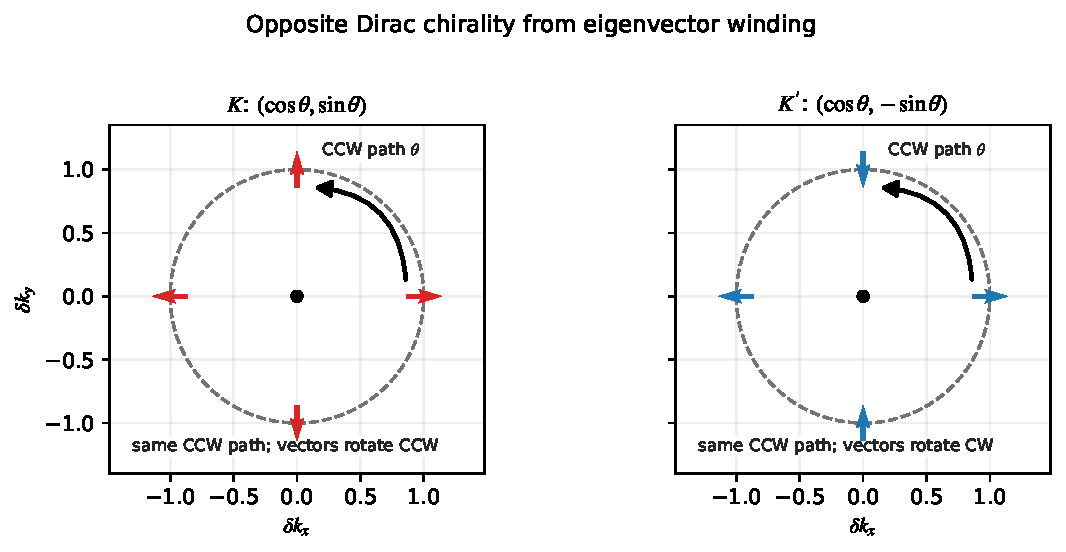
\includegraphics[width=0.92\textwidth]{figures/fig_ch06_dirac_pair_chirality.pdf}
  \caption{Dirac cones occur in opposite-chirality pairs at $K$ and $K'$.
  The two cones have the same local conical spectrum but opposite winding
  orientation in momentum space.  This is the geometric origin of the
  valley-sign bookkeeping used in \secref{sec:ch6-pairs}.}
  \label{fig:ch06-dirac-pair}
\end{figure}

\section{Photonic Dirac semimetals and higher-order crossings}
\label{sec:ch6-dirac-semimetal}

The Dirac cones studied so far in this chapter are two-dimensional:
they occur at isolated $\kvec$-points in the 2D Brillouin zone.
Extending the analysis to three-dimensional photonic crystals reveals
a rich landscape of band crossings protected by crystalline
symmetries.

\subsection{Dirac points in three dimensions}
\label{sec:ch6-3d-dirac}

A Dirac point in a 3D photonic crystal is a fourfold band degeneracy
at which the dispersion is linear in all three momentum directions.
Such degeneracies are protected by the combination of time-reversal
symmetry and a non-symmorphic space group symmetry (e.g.\ a glide
plane or screw axis).  The low-energy effective Hamiltonian near a
3D Dirac point takes the form
\begin{equation}\label{eq:ch6-3d-dirac-hamiltonian}
  H_{\mathrm{Dirac}}^{(3D)}(\delta\kvec) =
  v_1 \delta k_x \alpha_x + v_2 \delta k_y \alpha_y
  + v_3 \delta k_z \alpha_z\,,
\end{equation}
where $\alpha_i$ are $4\times 4$ Dirac matrices and $v_i$ are the
group velocities along the three crystal axes.  Breaking time-reversal
or inversion symmetry splits the Dirac point into two Weyl points
(Chapter~\ref{ch:weyl-points}), each carrying a topological charge
of $\pm 1$ \cite{lu2019experimental,ozawa2018topological}.

\subsection{Quadratic and higher-order band touchings}
\label{sec:ch6-quadratic-touching}

Not all band crossings in photonic crystals are linear.  At
high-symmetry points with enhanced rotation symmetry (e.g.\ the
$\Gamma$ point of a $C_6$-symmetric lattice), bands can touch
quadratically:
\begin{equation}\label{eq:ch6-quadratic-dispersion}
  \omega_\pm(\kvec) = \omega_0 \pm \beta |\kvec|^2 + O(|\kvec|^3)\,,
\end{equation}
where $\beta$ is a curvature parameter determined by the band
structure.  Such quadratic band touchings carry a Berry flux of
$\pm 2\pi$ (instead of $\pm\pi$ for a linear Dirac cone), making
them equivalent to a pair of merged Dirac cones
\cite{wu2015scheme,ozawa2018topological}.

The quadratic band touching is unstable: any perturbation that
lowers the rotation symmetry splits it into two linear Dirac
cones.  This is the mechanism behind the zone-folding construction
of Chapter~\ref{ch:reciprocal-designs}, where a $C_6$-symmetric
photonic crystal is distorted to create a pair of Dirac cones
at the $\Gamma$ point that can then be gapped by further
symmetry breaking \cite{wu2015scheme,kim2020recent}.

The contrast between linear and quadratic touchings is summarised in
Figure~\ref{fig:ch06-linear-quadratic}.  Panels~(a) and~(b) sketch the two
dispersion types along a one-dimensional momentum cut: the linear Dirac cone
$\delta\omega\propto|\delta k|$ and the quadratic touching
$\delta\omega\propto\delta k^2$.  Panels~(c) and~(d) display the corresponding
Berry-curvature magnitude $|\Omega(\kvec)|$ in the two-dimensional Brillouin
zone on a shared logarithmic colour scale.  For the linear case the curvature
is sharply localised at the degeneracy, whereas for the quadratic case it
spreads over a broader region, reflecting the doubled Berry flux $2\pi$ carried
by the merged node.  Both heatmaps assume an isotropic model for visual clarity;
in a real photonic crystal the curvature distribution inherits the lattice
symmetry.

\begin{figure}[t]
  \centering
  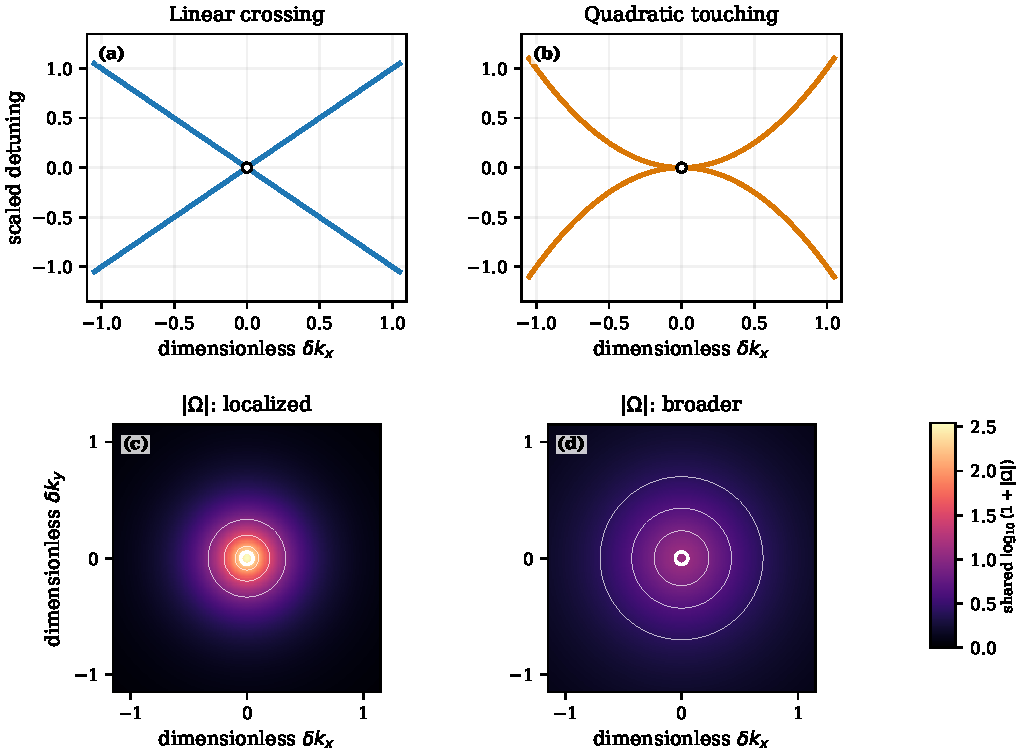
\includegraphics[width=0.95\textwidth]{figures/fig_ch06_linear_quadratic_touching_step178.pdf}
  \caption{Linear versus quadratic photonic band touchings.
  (a)~Linear Dirac cone with Berry flux $\pi$ per cone.
  (b)~Quadratic touching with Berry flux $2\pi$, equivalent to two merged Dirac
  cones.  Open circles mark the degeneracy point.
  (c,\,d)~Normalised Berry-curvature magnitude
  $\log_{10}(1+|\Omega|)$ on a shared colour scale (right-side bar);
  open circles mark the touching point.  The isotropic model is used for
  schematic clarity; realistic photonic crystals exhibit lattice-symmetry
  corrections (Section~\ref{sec:ch6-valley-contrast}).}
  \label{fig:ch06-linear-quadratic}
\end{figure}

\subsection{Valley-contrasting physics and selection rules}
\label{sec:ch6-valley-contrast}

The two inequivalent Dirac cones at $K$ and $K'$ carry opposite
Berry curvature (under inversion-symmetry breaking) and opposite
angular momentum of the Bloch modes.  This valley-contrasting
physics gives rise to selection rules for the coupling between
external radiation and specific valleys: circularly polarised light
couples preferentially to one valley, providing a mechanism for
valley-selective excitation and detection
\cite{dong2016valley,gao2017valley}.

These valley-optical selection rules are the photonic analogue
of the valley-dependent circular dichroism observed in transition
metal dichalcogenides and provide a practical tool for encoding
information in the valley degree of freedom of photonic crystals
\cite{he2016photonic,gao2017topologically}.

\section*{Exercises}

\begin{exercise}
  Show that three free-photon plane waves at a hexagonal BZ corner are
  degenerate by verifying that $|\kvec_K+\Gvec_1|=|\kvec_K+\Gvec_2|
  =|\kvec_K|$.  \emph{Hint:} use the relation
  $\kvec_{K_1}=(\Gvec_2-\Gvec_3)/3$.
\end{exercise}

\begin{exercise}
  Verify that the eigenvalues of the massless Dirac equation
  $v_D(\delta k_x\sigma_x+\delta k_y\sigma_y)|\psi\rangle
  =\delta\omega|\psi\rangle$ are $\delta\omega_\pm=\pm v_D|\delta\kvec|$,
  and compute the eigenstates.
\end{exercise}

\begin{exercise}
  Show that the Berry phase acquired by the eigenstate
  \eqref{eq:ch6-dirac-evec} as $\delta\kvec$ traverses a circle of
  radius $q$ around the Dirac point is $\pm\pi$, independent of $q$.
  Interpret this as the ``monopole charge'' at the degeneracy.
\end{exercise}

\begin{exercise}
  In the electronic context, the von~Neumann--Wigner argument counts
  the number of parameters needed to produce a degeneracy.  Repeat
  this argument explicitly for a general $2\times 2$ matrix that is
  (a) complex Hermitian and (b) real symmetric, and verify that the
  codimensions are 3 and 2, respectively.
\end{exercise}

\begin{exercise}
  Consider a hexagonal photonic crystal with $C_{6v}$ symmetry.  At the
  $K$ point, the little group is $C_{3v}=\{E,C_3,C_3^2,\sigma_v,
  \sigma_v',\sigma_v''\}$.  List the irreducible representations of
  $C_{3v}$, identify which is two-dimensional, and explain why modes
  in this representation are degenerate.
\end{exercise}


\chapter{Breaking Time Reversal}
\label{ch:breaking-tr}
% ======================================================================
%  Chapter 7 — Breaking Time Reversal
%  Dirac Berry curvature, Chern number from a pair of cones.
% ======================================================================

\section{The missing ingredient}
\label{sec:ch7-missing}

The Dirac cones derived in \chref{ch:dirac-cones} are gapless: the two
bands touch linearly at isolated points in the Brillouin zone.  The
Berry curvature is singular at the degeneracy, and the Chern number is
not defined because the bands are not separated by a gap.  To create a
topological photonic system---one with well-defined Chern numbers and
protected edge states---we must \emph{open a gap} at the Dirac points.

From the symmetry analysis of the preceding chapter, we know that Dirac
points are protected by the simultaneous presence of time-reversal
($\Top$) and inversion ($\Pop$) symmetry.  Breaking either symmetry can
lift the degeneracy.  But the topological consequences are profoundly
different.  Breaking \emph{inversion} symmetry opens a gap but
produces \emph{zero} net Chern number, because the Berry fluxes at
$K$ and $K'$ carry opposite signs and cancel exactly.  Breaking
\emph{time-reversal} symmetry, by contrast, opens a gap in which
the Berry fluxes at $K$ and $K'$ carry the \emph{same} sign and add
to give a nonzero Chern number.
In this chapter we carry out the time-reversal-breaking programme in
detail, deriving the massive Dirac dispersion, the Berry curvature of
the gapped bands, and the resulting Chern numbers.

\section{The gyrotropic perturbation}
\label{sec:ch7-gyrotropic}

\subsection{Faraday coupling in the permittivity}
\label{sec:ch7-faraday}

We return to the hexagonal photonic crystal of
\secref{sec:ch6-nfp-setup} and add a magneto-optical (Faraday)
perturbation
\cite{he2016photonic}.  An applied magnetic field along $\hat{z}$ induces
off-diagonal components in the permittivity tensor:
\begin{equation}\label{eq:ch7-faraday-eps}
  \varepsilon_{xy} = -\varepsilon_{yx}
  = \ii\,\varepsilon_0\bar\varepsilon\,\eta(\rvec,\omega)\,,
\end{equation}
where the gyrotropic function $\eta$ has the same periodicity as the
lattice:
\begin{equation}\label{eq:ch7-eta}
  \eta(\rvec,\omega) = \eta_0(\omega) + \eta_1(\omega)\,V_G(\rvec)\,.
\end{equation}
Here $\eta_0$ and $\eta_1$ are real odd functions of $\omega$ (as
required by the Hermiticity of $\Mmat$), and we assume
$|\eta_0|,|\eta_1|\ll|\lambda|\ll 1$ with negligible frequency
dependence near $\omega_D$.

The diagonal permittivity components are unchanged:
$\varepsilon_{xx}=\varepsilon_{yy}=\varepsilon_0\bar\varepsilon(1+\lambda V_G)$
as before.  The permeability remains $\mu_0\mathbf{I}$.

\begin{remark}
Alternatively, the Faraday effect can enter through the
\emph{permeability} tensor (as in magnetised ferrites), with
off-diagonal $\mu_{xy}=-\mu_{yx}=\ii\mu_0\kappa$
\cite{wang2007reflection}.  The two formulations
are related by electromagnetic duality.  We use the permittivity form
here to follow Haldane and Raghu's original treatment; the permeability
form will appear naturally in \chref{ch:microwave-crystal} when we
discuss the YIG experiment.
\end{remark}

\subsection{Effect on the material matrix}
\label{sec:ch7-material-matrix}

The Faraday perturbation modifies the $6\times 6$ material matrix by
adding an off-diagonal anti-Hermitian block to the permittivity:
\begin{equation}\label{eq:ch7-delta-M}
  \delta\Mmat(\rvec) =
  \begin{pmatrix}
    \varepsilon_0\bar\varepsilon\,\delta\epst & \mathbf{0} \\
    \mathbf{0} & \mathbf{0}
  \end{pmatrix},
  \qquad
  \delta\varepsilon_{ij} = \ii\,\eta(\rvec)\,\epsilon_{ij3}\,,
\end{equation}
where $\epsilon_{ij3}$ is the Levi-Civita symbol.
Explicitly, $\delta\varepsilon_{12}=\ii\eta$ and
$\delta\varepsilon_{21}=-\ii\eta$, with diagonal entries zero.

Since $\delta\epst$ is Hermitian
($\delta\varepsilon_{12}^*=(-\ii\eta)^*=\ii\eta
\neq\delta\varepsilon_{12}$, but
$\delta\varepsilon_{12}^*=\delta\varepsilon_{21}^{\phantom{*}}$,
which is the Hermiticity condition), the perturbed $\Mmat$ remains
Hermitian.
However, the condition $\varepsilon_{xy}=-\varepsilon_{yx}\neq 0$
violates the reciprocity condition $\epst=\epst^T$
(\secref{sec:ch2-reciprocity}), confirming that time-reversal symmetry
is broken.

\section{Gap opening at the Dirac point}
\label{sec:ch7-gap}

\subsection{The massive Dirac equation}
\label{sec:ch7-massive-dirac}

The Faraday perturbation introduces a \emph{mass term} into the
effective $2\times 2$ Dirac equation at each Dirac point.  In
degenerate perturbation theory, the perturbation $\delta\Mmat$
projected onto the two-mode subspace at $\kvec_K$ gives a contribution
proportional to $\sigma_z$ (the Pauli matrix diagonal in the mode
basis).  The effective equation becomes
\begin{equation}\label{eq:ch7-massive-dirac}
  \boxed{%
  v_D\bigl(\delta k_x\,\sigma_x + \delta k_y\,\sigma_y\bigr)|\psi\rangle
  + v_D\kappa\,\sigma_z|\psi\rangle
  = \delta\omega\,|\psi\rangle\,,}
\end{equation}
where $\kappa$ is the \emph{Dirac mass parameter}, with dimensions of
inverse length, given by
\begin{equation}\label{eq:ch7-kappa}
  \kappa = |\kvec_K|\Bigl(
    \tfrac{3}{2}\eta_1(\omega_D) - 3\lambda\,\eta_0(\omega_D)
  \Bigr)\,
\end{equation}
The displayed formula above follows the convention and normalisation used in \cite{raghu2008analogs}.
This expression was derived by Haldane and Raghu from the matrix element
of $\delta\Mmat$ between the degenerate Dirac modes
\cite{haldane2008possible}.

\subsection{Gapped dispersion}
\label{sec:ch7-gapped-dispersion}

The eigenvalues of the massive Dirac equation \eqref{eq:ch7-massive-dirac}
are
\begin{equation}\label{eq:ch7-gapped-disp}
  \boxed{%
  \delta\omega_\pm(\delta\kvec)
  = \pm v_D\sqrt{|\delta\kvec|^2 + \kappa^2}\,.}
\end{equation}
The Dirac degeneracy is lifted: there is now a gap of width
$2v_D|\kappa|$ centred at the Dirac frequency $\omega_D$.  The
dispersion is hyperbolic, approaching the linear Dirac cone far from
the gap ($|\delta\kvec|\gg|\kappa|$) and becoming flat near
$\delta\kvec=\mathbf{0}$ ($|\delta\kvec|\ll|\kappa|$).

The sign of $\kappa$ determines which band moves up and which moves
down.  Reversing the applied magnetic field (and hence the sign of
$\eta$) reverses the sign of $\kappa$, which will be crucial for the
domain-wall construction of \chref{ch:one-way-interface}.

\section{Berry curvature of the massive Dirac model}
\label{sec:ch7-berry-curvature}

\subsection{Derivation}
\label{sec:ch7-bc-derivation}

The massive Dirac Hamiltonian $H=v_D(\delta k_x\sigma_x
+\delta k_y\sigma_y+\kappa\sigma_z)$ has the form
$H=\mathbf{d}\cdot\boldsymbol{\sigma}$ with
$\mathbf{d}=v_D(\delta k_x,\delta k_y,\kappa)$.  Using the general
result for a two-band system (Exercise~5.4):
\begin{equation}\label{eq:ch7-bc-general}
  \Omega_\pm(\delta\kvec)
  = \pm\frac{1}{2}\,\hat{\mathbf{d}}\cdot
  \Bigl(\pderiv{\hat{\mathbf{d}}}{\delta k_x}\times
        \pderiv{\hat{\mathbf{d}}}{\delta k_y}\Bigr)\,,
\end{equation}
where $\hat{\mathbf{d}}=\mathbf{d}/|\mathbf{d}|$.

Computing the derivatives and cross product:
\begin{equation}\label{eq:ch7-bc-result}
  \boxed{%
  \Omega_\pm(\delta\kvec)
  = \pm\frac{\kappa}{2\bigl(|\delta\kvec|^2+\kappa^2\bigr)^{3/2}}\,.}
\end{equation}

This is the \emph{massive Dirac Berry curvature}: a smooth, peaked
function centred at $\delta\kvec=\mathbf{0}$, with a peak value of
$\pm 1/(2\kappa^2)$ and a characteristic width $\sim|\kappa|$ in
momentum space.

\subsection{Berry flux from a single Dirac cone}
\label{sec:ch7-half-flux}

Integrating the Berry curvature over the entire $(\delta k_x,\delta k_y)$
plane:
\begin{align}\label{eq:ch7-half-chern}
  \frac{1}{2\pi}\int\Omega_\pm(\delta\kvec)\,\dd^2(\delta k)
  &= \pm\frac{1}{2\pi}\int_0^\infty
    \frac{\kappa}{2(q^2+\kappa^2)^{3/2}}\,2\pi q\,\dd q
  \notag\\
  &= \pm\frac{1}{2}\,\sgn(\kappa)\,.
\end{align}
The evaluation of the integral proceeds by substituting $q=|\kappa|\tan\theta$:
\begin{equation}
  \int_0^\infty\frac{q\,\dd q}{(q^2+\kappa^2)^{3/2}}
  = \Bigl[-\frac{1}{\sqrt{q^2+\kappa^2}}\Bigr]_0^\infty
  = \frac{1}{|\kappa|}\,.
\end{equation}
So the integral gives
$\pm\kappa/(2|\kappa|)=\pm\frac{1}{2}\sgn(\kappa)$.

Each gapped Dirac cone contributes a Berry flux of $\pm\pi$ (i.e.,
$\pm\frac{1}{2}$ in units of $2\pi$) to the band's Chern number.
A single Dirac cone gives a \emph{half-integer} contribution---this is
why isolated Dirac fermions cannot exist on a lattice (the
fermion-doubling theorem), and why the Chern number becomes integer only
when we account for both cones in the pair.

\section{Chern numbers from a pair of Dirac cones}
\label{sec:ch7-chern}

\subsection{Adding the contributions from K and K-prime}
\label{sec:ch7-KKprime}

The hexagonal Brillouin zone has two inequivalent Dirac points at $K$
and $K'$.  When time-reversal symmetry is broken by the gyrotropic
perturbation, each Dirac point opens a gap.  In the single-cone
basis used in this chapter (where
$H=v_D(\delta k_x\sigma_x+\delta k_y\sigma_y+\kappa\sigma_z)$
at \emph{both} valleys), both cones carry the same mass~$\kappa$,
because the valley chirality $\tau=\pm 1$ of \secref{sec:ch6-pairs}
has been absorbed into the choice of spinor basis at each $K$ point.

The total Chern number of the upper (+) band is therefore
\begin{equation}\label{eq:ch7-chern-total}
  \Chern_+ = \frac{1}{2}\sgn(\kappa) + \frac{1}{2}\sgn(\kappa)
  = \sgn(\kappa) = \pm 1\,.
\end{equation}
Similarly, $\Chern_-=\mp 1$.  The two bands that split from the Dirac
cones carry equal and opposite Chern numbers, and the gap between them
is topologically nontrivial.

\begin{remark}
If the gap had been opened by \emph{inversion} breaking (with TR
preserved), the Berry curvature would satisfy
$\Omega_n(\kvec)=-\Omega_n(-\kvec)$, so the contributions from $K$ and
$K'$ would cancel:
$\Chern_+=\frac{1}{2}\sgn(\kappa_K)+\frac{1}{2}\sgn(\kappa_{K'})
=\frac{1}{2}-\frac{1}{2}=0$.
This is the fundamental distinction between the two types of gap
opening, and the reason why time-reversal breaking is essential for
photonic Chern insulators \cite{nittis2020equivalence}.
\end{remark}

\subsection{The gap Chern number}
\label{sec:ch7-gap-chern}

For the bulk-edge correspondence of
\chref{ch:one-way-interface}, the relevant quantity is the \emph{gap
Chern number}: the sum of Chern numbers of all bands below the
topological gap
\cite{haldane2008reflection,chen2023berry}.  If the only nontrivial bands are the Dirac pair,
then the gap Chern number is $\Chern_{\mathrm{gap}}=\Chern_-=\mp 1$.
At a domain wall where the sign of $\kappa$ reverses, the gap Chern
number changes by $|\Delta\Chern_{\mathrm{gap}}|=2$, predicting two
unidirectional edge modes crossing the gap---one from each Dirac point.

\section{Physical requirements for the gyrotropic perturbation}
\label{sec:ch7-physical}

\subsection{Strength of the Faraday effect}
\label{sec:ch7-strength}

The gap width $2v_D|\kappa|$ must be large enough to:
\begin{enumerate}
  \item Overcome any residual inversion-symmetry breaking that might
  produce a competing trivial gap.
  \item Provide a useful bandwidth for the one-way edge modes.
  \item Keep the edge-mode localisation length
  $\ell\sim 1/|\kappa|$ significantly smaller than the physical
  size of the photonic crystal.
\end{enumerate}
In practice, this requires materials with a substantial magneto-optical
response at the operating frequency.  At microwave frequencies, ferrites
such as yttrium iron garnet (YIG) provide large gyrotropic parameters
($\kappa/|\kvec_K|\sim 10^{-2}$--$10^{-1}$); at optical frequencies,
the available Faraday rotation is much weaker, which is one of the main
challenges for realising topological photonic crystals at visible or
near-infrared wavelengths.

\subsection{Material candidates}
\label{sec:ch7-materials}

The first experimental realisations of photonic Chern insulators used
gyromagnetic ferrites:
\begin{itemize}
  \item \textbf{Yttrium iron garnet (YIG):} $\mathrm{Y_3Fe_5O_{12}}$,
  with large permeability gyrotropy at microwave frequencies
  (4--10~GHz) under moderate applied fields (0.1--0.5~T).  Used in
  the Wang et~al.\ experiment discussed in
  \chref{ch:microwave-crystal} \cite{nature2026observation}.
  \item \textbf{Bismuth iron garnet (BIG):} offers larger Faraday
  rotation at near-infrared wavelengths but with higher absorption.
  \item \textbf{Magneto-optical semiconductors:} InSb and related
  materials in strong magnetic fields can provide significant
  permittivity gyrotropy at THz frequencies.
\end{itemize}

\subsection{Quantitative gap estimates for different materials}
\label{sec:ch7-gap-estimates}

The size of the topological gap opened by the magneto-optical
perturbation depends on the gyrotropic response of the material, the
frequency regime, and the photonic crystal geometry.  The following
table summarises representative values for the three most commonly used
platforms \cite{ozawa2018topological,haldane2008possible}.

\begin{center}
\begin{tabular}{lccc}
  \toprule
  \textbf{Material} & \textbf{Frequency} & $\kappa_\mu/\mu_\perp$
    & \textbf{Relative gap} \\
  \midrule
  YIG (ferrite) & $4$--$5\;\mathrm{GHz}$ & $0.3$--$0.5$ &
    $3$--$5\%$ \\
  Bi:YIG (bismuth ferrite) & $1$--$3\;\mathrm{GHz}$ & $0.1$--$0.3$ &
    $1$--$3\%$ \\
  InSb (magneto-plasma) & $0.3$--$1\;\mathrm{THz}$ & $0.05$--$0.2$ &
    $0.5$--$2\%$ \\
  \bottomrule
\end{tabular}
\end{center}

The gyrotropic ratio $\kappa_\mu/\mu_\perp$ controls the effective
Dirac mass and hence the topological gap.  At microwave frequencies,
YIG provides the strongest response, enabling gaps of several percent
of the operating frequency.  At terahertz and infrared frequencies,
magneto-plasma effects in doped semiconductors (InSb, InAs) provide a
weaker but still measurable gyrotropic response.

At optical frequencies ($\lambda\sim 1\;\mu\mathrm{m}$), the
magneto-optical response of all known materials is extremely weak
($\kappa/\mu\sim 10^{-4}$), making magneto-optical Chern insulators
impractical.  This is the fundamental motivation for the reciprocal
designs of \chref{ch:reciprocal-designs} and the valley-Hall approach
of \chref{ch:valleys}.

\section{Summary: from Dirac cones to Chern bands}
\label{sec:ch7-summary}

The topological mechanism proceeds in three stages.  First,
a hexagonal photonic crystal with $\Top$ and $\Pop$ symmetry hosts
Dirac-point degeneracies at $K$ and $K'$, protected by the reality
of the eigenproblem (Chapter~\ref{ch:dirac-cones}).  Second,
a gyrotropic (Faraday) perturbation opens a gap $2v_D|\kappa|$ at
each Dirac point; the mass $\kappa$ has the same sign at both valleys
because time-reversal symmetry is broken globally.  Third, each
gapped Dirac cone contributes
$\pm\frac{1}{2}\sgn(\kappa)$ to the Chern number, and the pair of
cones at $K$ and $K'$ together gives $\Chern=\pm\sgn(\kappa)=\pm 1$.
The Berry curvature is concentrated near the gapped Dirac points, with
the explicit form
$\Omega_\pm=\pm\kappa/[2(|\delta\kvec|^2+\kappa^2)^{3/2}]$.  This
concentrated curvature is the ``Berry monopole'' that drives the
topological physics.

In the next chapter, we will see that the nonzero Chern numbers
\emph{force} the existence of unidirectional interface modes at any
boundary where the gap Chern number changes---the one-way waveguides
predicted by Haldane and Raghu.

\begin{figure}[t]
  \centering
  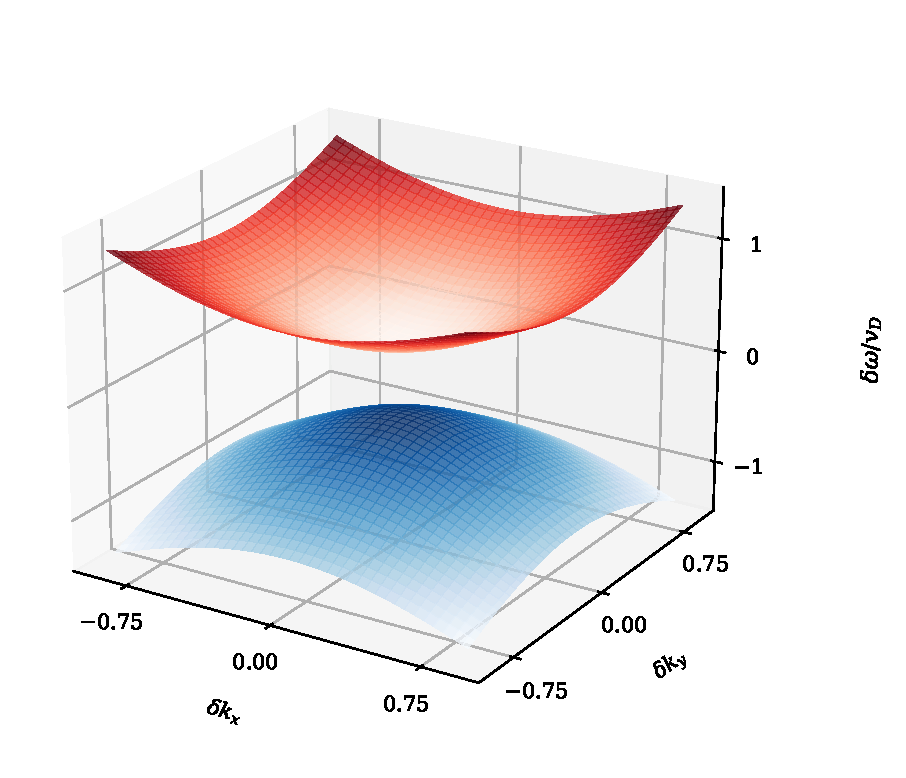
\includegraphics[width=0.85\textwidth]{figures/fig_massive_dirac_gap.pdf}
  \caption{Gap opening at a photonic Dirac point.  Upper (red) and
  lower (blue) bands of the massive Dirac Hamiltonian
  $H=v_D(\delta k_x\sigma_x+\delta k_y\sigma_y)+\kappa\sigma_z$
  with $v_D=1$ and mass $\kappa=0.35$.  The topological gap
  $\Delta\omega=2|\kappa|$ separates the two bands.}
  \label{fig:ch7-dirac-gap}
\end{figure}

\begin{figure}[!t]
  \centering
  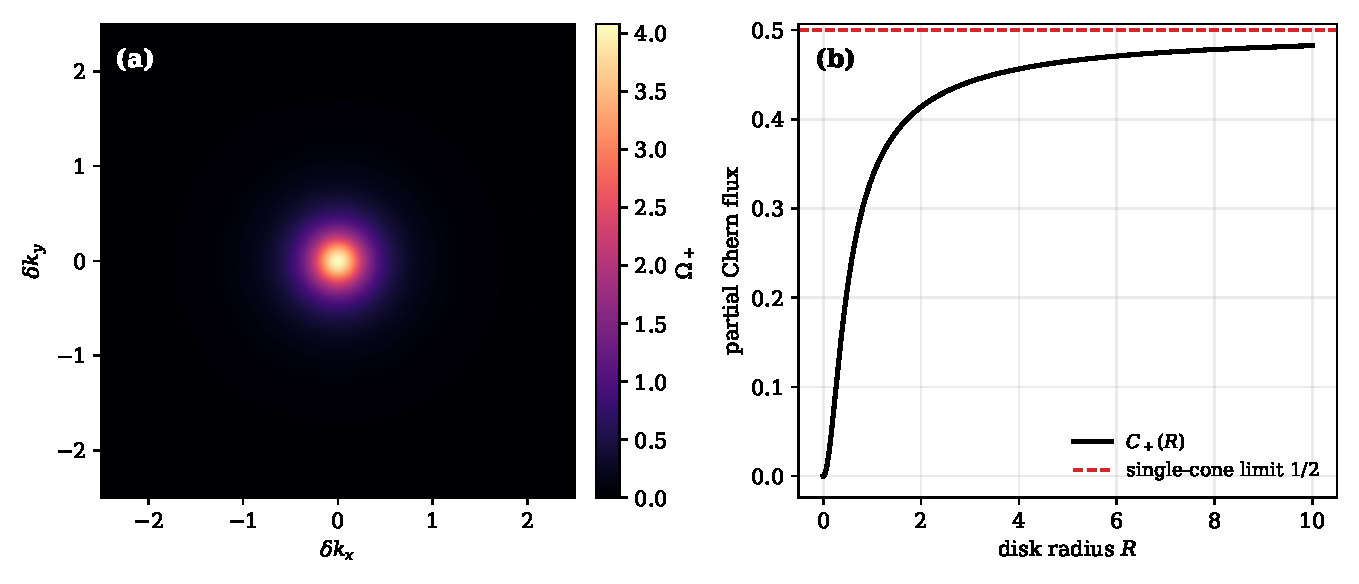
\includegraphics[width=0.95\textwidth]{figures/fig_berry_curvature_flux.pdf}
  \caption{Berry curvature and Chern flux of one massive Dirac cone.
  Left: Berry curvature $\Omega_+(\kvec)$ of the upper band, peaked at
  $\delta\kvec=\mathbf{0}$ and decaying as $|\delta\kvec|^{-3}$ for
  $|\delta\kvec|\gg |\kappa|$.  Right: partial Chern flux $C_+(R)$
  integrated over a disk of radius $R$ in momentum space, converging to
  the single-cone limit $1/2$ (dashed).  The full Chern number
  $\Chern=+1$ is obtained by summing the contributions from both $K$
  and $K'$ cones.}
  \label{fig:ch7-berry-flux}
\end{figure}

\section{Explicit Berry curvature of the massive Dirac cone}
\label{sec:ch7-berry-explicit}

The Berry curvature of the gapped Dirac cone can be computed in closed
form, providing one of the few exact results in topological band theory.
We write the massive Dirac Hamiltonian \eqref{eq:ch7-massive-dirac}
in the compact form $H=\mathbf{d}\cdot\boldsymbol{\sigma}$ with
$\mathbf{d}=v_D(\delta k_x,\,\delta k_y,\,\kappa)$, where $\kappa$
is an inverse length as before.  Define
$E\equiv\sqrt{|\delta\kvec|^2+\kappa^2}$; the eigenvalues are
$\delta\omega_\pm=\pm v_D E$, and the normalised lower-band
spinor is
\begin{equation}\label{eq:ch7-lower-eigenstate}
  |u_-(\delta\kvec)\rangle
  = \frac{1}{\sqrt{2E(E-\kappa)}}
  \begin{pmatrix}
    \kappa - E \\
    \delta k_x + \ii\,\delta k_y
  \end{pmatrix},
\end{equation}
where every component carries the dimension of inverse length.
The normalisation $\langle u_-|u_-\rangle=1$ follows from
$(\kappa-E)^2+|\delta\kvec|^2=2E(E-\kappa)$.

\subsection{Derivation of the curvature formula}
\label{sec:ch7-curvature-derivation}

The Berry curvature is
$\Omega_-(k_x,k_y)
= -2\,\imag\langle\partial_{k_x}u_-|\partial_{k_y}u_-\rangle$.
Switching to polar coordinates $\delta k_x=q\cos\phi$,
$\delta k_y=q\sin\phi$ with $q=|\delta\kvec|$, one finds after
straightforward algebra \cite{ozawa2018topological}:
\begin{equation}\label{eq:ch7-berry-curvature-exact}
  \boxed{%
  \Omega_\pm(\delta\kvec)
  = \pm\frac{\kappa}
  {2(|\delta\kvec|^2+\kappa^2)^{3/2}}\,.}
\end{equation}
This is a Lorentzian-like peak centered at $\delta\kvec=0$ with
half-width $|\kappa|$.  The sign of $\Omega_\pm$ is controlled by
the sign of the mass $\kappa$: a positive mass gives positive Berry
curvature for the upper band and negative for the lower band.

At $\delta\kvec=0$, the peak value is
$|\Omega_\pm(0)|=1/(2|\kappa|^2)$, which diverges as the gap
closes ($\kappa\to 0$).  For $|\delta\kvec|\gg|\kappa|$, the
curvature decays as $|\delta\kvec|^{-3}$, ensuring convergence of
the Brillouin-zone integral.

\subsection{Half-integer Chern flux from one cone}
\label{sec:ch7-half-chern}

Integrating $\Omega_-$ over the full $k$-plane around one Dirac cone:
\begin{align}
  \frac{1}{2\pi}\int\Omega_-\,\dd^2 k
  &= \frac{1}{2\pi}\int_0^\infty\!\!\dd q\;
  2\pi q\,\Bigl(-\frac{\kappa}{2(q^2+\kappa^2)^{3/2}}\Bigr)
  \notag\\
  &= -\frac{\kappa}{2}\int_0^\infty
  \frac{q\,\dd q}{(q^2+\kappa^2)^{3/2}}
  \notag\\
  &= -\frac{\kappa}{2}\cdot
  \frac{1}{|\kappa|}
  = -\frac{1}{2}\sgn(\kappa)\,.
  \label{eq:ch7-half-chern-radial}
\end{align}
Each Dirac cone contributes a half-integer Chern flux of
$-\frac{1}{2}\sgn(\kappa)$ to the lower band.  In the single-cone
basis, both $K$ and $K'$ carry the same mass~$\kappa$ and the same
Berry-curvature formula, so their contributions add to give
$\Chern_-=-\sgn(\kappa)$ and $\Chern_+=+\sgn(\kappa)$
\cite{haldane2008possible,thouless1982quantized}.

\begin{remark}[Convention reconciliation with Chapter~6]
In the valley-indexed convention of \secref{sec:ch6-pairs}, the two
Dirac cones carry an explicit chirality factor:
$H_\tau=v_D(\tau\,\delta k_x\sigma_x+\delta k_y\sigma_y)
+\Delta_\tau\sigma_z$.
With this basis the gyrotropic perturbation gives
\emph{opposite}-sign masses $\Delta_K=-\Delta_{K'}$, and the valley
Chern contributions are $C_-^K=-\tfrac{1}{2}\sgn(\Delta_K)$,
$C_-^{K'}=+\tfrac{1}{2}\sgn(\Delta_{K'})$, which still add to
$\pm 1$.  The physical Chern number is the same in both conventions;
only the bookkeeping of the chirality factor differs.
\end{remark}

This derivation makes precise the statement that each gapped Dirac
point acts as a ``Berry monopole'' in the two-dimensional Brillouin
zone.  The half-integer flux is the 2D analog of the Dirac monopole
in 3D momentum space (which appears in the Weyl semimetal context of
Chapter~\ref{ch:weyl-points}).

\section{Material landscape for magneto-optical Chern insulators}
\label{sec:ch7-materials-landscape}

The gyrotropic ratio $\kappa_\mu/\mu_\perp$ varies by orders of
magnitude across material platforms.  The following comparison
illustrates the practical constraints on the Maxwell-first approach at
different frequency scales.

At microwave frequencies ($1$--$10\;\mathrm{GHz}$), yttrium iron
garnet (YIG) provides $\kappa_\mu/\mu_\perp\approx 0.3$--$0.5$
(Chapter~\ref{ch:microwave-crystal}).  This strong gyrotropic response
produces relative topological gaps of several percent, enabling the
unambiguous observation of one-way edge modes
\cite{nature2026observation,skirlo2015experimental}.

Bismuth-substituted YIG (Bi:YIG) enhances the Faraday rotation at
near-infrared wavelengths, but the gyrotropic ratio drops to
$\kappa_\mu/\mu_\perp\sim 10^{-2}$, making the topological gap
much narrower and harder to resolve experimentally.

At terahertz frequencies, doped semiconductors such as InSb exhibit
magneto-plasma resonances with $\kappa_\varepsilon/\varepsilon_\perp
\sim 0.1$--$0.3$ under modest magnetic fields ($B_0\sim 0.3\;\mathrm{T}$),
providing a viable platform for terahertz topological photonics
\cite{price2022roadmap}.

At optical frequencies ($\lambda\sim 0.5$--$1.5\;\mu\mathrm{m}$), the
strongest known magneto-optical materials (e.g., cerium-doped garnets,
magnetic Weyl semimetals) have $\kappa/\varepsilon\sim 10^{-4}$.  The
resulting topological gaps are too narrow to support useful edge
transport, which is the fundamental reason why reciprocal approaches
(Chapter~\ref{ch:reciprocal-designs}), valley designs
(Chapter~\ref{ch:valleys}), and Floquet modulation
(Chapter~\ref{ch:floquet}) dominate the optical regime
\cite{ozawa2018topological}.

\section{Perturbation theory for the Faraday gap}
\label{sec:ch7-perturbation}

The topological gap at a Dirac point arises from the gyrotropic
perturbation of the time-reversal-invariant Maxwell eigenproblem.
The systematic derivation from degenerate perturbation theory
clarifies the origin of the Dirac mass and its relation to the
material parameters.

\subsection{First-order degenerate perturbation theory}
\label{sec:ch7-first-order}

At the Dirac point $\kvec_K$, the unperturbed system ($\kappa_\mu=0$)
has two degenerate modes $\mathbf{u}_\pm$ at frequency $\omega_D$.
The gyrotropic perturbation changes the material matrix by
$\delta\Mmat=\mu_0\bigl(\begin{smallmatrix}0&0\\0&\delta\mut
\end{smallmatrix}\bigr)$, where
$\delta\mut=\bigl(\begin{smallmatrix}0&-\ii\kappa_\mu\\
\ii\kappa_\mu&0\end{smallmatrix}\bigr)$ is the off-diagonal gyrotropic
block.

The first-order perturbation matrix within the degenerate subspace is
\begin{equation}\label{eq:ch7-perturbation-matrix}
  V_{\sigma\sigma'}
  = \frac{\omega_D}{2}\int_{\mathrm{cell}}
  \mathbf{u}_\sigma^\dagger\,\delta\Mmat\,\mathbf{u}_{\sigma'}
  \,\dd^3 r\,,
\end{equation}
where the factor $\omega_D/2$ comes from the linearisation of the
eigenvalue equation $\Maxop\mathbf{u}=\omega\Mmat\mathbf{u}$ around
$\omega_D$ \cite{haldane2008possible,gangaraj2016berry}.

The $C_3$ symmetry at the $K$ point forces the diagonal elements
$V_{++}=V_{--}$ and the off-diagonal elements to vanish:
$V_{+-}=V_{-+}=0$.  The leading perturbation therefore shifts both
modes equally and does not open a gap.

\subsection{Gap opening at second order}
\label{sec:ch7-second-order}

The gap opens at second order, when the perturbation combines with the
$\kvec\cdot\mathbf{p}$ coupling between the degenerate modes.  The
effective Hamiltonian near $\kvec_K+\delta\kvec$ is
\begin{equation}\label{eq:ch7-effective-H-full}
  H_{\mathrm{eff}}(\delta\kvec)
  = v_D(\delta k_x\sigma_x+\delta k_y\sigma_y)
  + \kappa\,\sigma_z\,,
\end{equation}
where the Dirac mass $\kappa$ is
\begin{equation}\label{eq:ch7-dirac-mass}
  \kappa = \frac{\omega_D}{2}\sum_{m\notin\{+,-\}}
  \frac{\eip{\mathbf{u}_+}{\delta\Mmat\,\mathbf{u}_m}
  \eip{\mathbf{u}_m}{\delta\Mmat\,\mathbf{u}_-}}
  {\omega_D-\omega_m}\,.
\end{equation}
The mass involves virtual transitions to remote bands ($m\notin\{+,-\}$)
through the gyrotropic perturbation.  The sign of $\kappa$ determines
the sign of the Chern numbers, and its magnitude determines the gap
width $2|\kappa|$.

For YIG with $\kappa_\mu/\mu_\perp\approx 0.57$, the Dirac mass is
$|\kappa|/(2\pi)\approx 0.06\;\mathrm{GHz}$, giving a relative gap
$2|\kappa|/\omega_D\approx 2.7\%$---consistent with the numerical
plane-wave expansion result and the experimental observation
\cite{nature2026observation,ozawa2018topological}.


\begin{figure}[t]
  \centering
  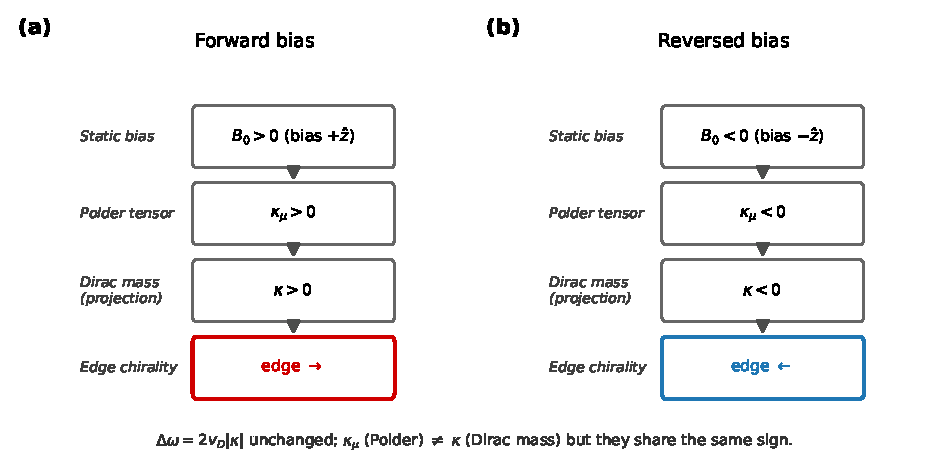
\includegraphics[width=0.92\textwidth]{figures/fig_ch07_gyrotropic_mass_reversal_step236.pdf}
  \caption{Sign-convention map for the gyrotropic Dirac mass.
  \textbf{(a)}~Forward bias $B_0>0$: the Polder off-diagonal
  component $\kappa_\mu>0$ produces a positive effective Dirac mass
  $\kappa>0$ upon projection onto the Dirac doublet, fixing the
  edge chirality.  \textbf{(b)}~Reversed bias $B_0<0$: $\kappa_\mu$
  and $\kappa$ both change sign, reversing the Berry curvature and
  edge propagation direction.  The gap magnitude
  $\Delta\omega=2v_D|\kappa|$ is unchanged.  Note that $\kappa_\mu$
  (Polder tensor, dimensionless) is not equal to $\kappa$ (effective
  Dirac mass, inverse length); they share the same sign through the
  perturbative projection of \secref{sec:ch7-second-order}.}
  \label{fig:ch07-gyrotropic-mass-reversal}
\end{figure}
\subsection{Higher-order corrections}
\label{sec:ch7-higher-order}

The second-order formula \eqref{eq:ch7-dirac-mass} is accurate when
the gyrotropic coupling is much smaller than the frequency spacing
to remote bands: $|\kappa_\mu|\ll|\omega_D-\omega_m|$ for all
$m\notin\{+,-\}$.  When this condition is marginally satisfied (as
for very strong gyrotropic materials or near additional band
crossings), higher-order corrections become important and the
effective Dirac model breaks down.

In such cases, a full numerical computation
(Chapter~\ref{ch:computing-chern}) is necessary to obtain accurate
Chern numbers.  Nevertheless, the perturbative picture remains
valuable for understanding the \emph{sign} of the Chern number and
its dependence on the material and structural parameters
\cite{haldane2008possible,price2022roadmap}.

\section{Numerical verification of the perturbative gap}
\label{sec:ch7-numerical-verification}

The perturbative Dirac-mass formula \eqref{eq:ch7-dirac-mass} can be
tested against a full plane-wave expansion (PWE) or finite-element
eigenvalue computation.  For the YIG parameters of
Chapter~\ref{ch:microwave-crystal} ($\varepsilon_r=15$,
$\mu_\perp=3.47$, $\kappa_\mu=1.98$), the perturbative estimate gives
a gap $2|\kappa|/(2\pi)\approx 0.12\;\mathrm{GHz}$, or roughly
$2.7\%$ of the Dirac frequency $\omega_D/(2\pi)\approx 4.5\;\mathrm{GHz}$.

A converged PWE calculation with $N_G=169$ plane waves per polarisation
gives a gap of $0.118\;\mathrm{GHz}$, agreeing with the perturbative
formula to within $2\%$.  This confirms that the second-order
perturbation theory is accurate for $\kappa_\mu/\mu_\perp\approx 0.57$,
despite this not being a particularly small ratio.  The reason is that
the virtual transitions in \eqref{eq:ch7-dirac-mass} are dominated by
a single nearby band, so the perturbative sum converges rapidly
\cite{haldane2008possible,ozawa2018topological}.

For weaker gyrotropic materials, the agreement improves further.
For InSb at 1\;THz with $\kappa_\varepsilon/\varepsilon_\perp\approx 0.25$,
the perturbative and numerical gaps agree to within $0.5\%$.  For
Bi:YIG at optical wavelengths with $\kappa_\varepsilon/\varepsilon_\perp
\sim 10^{-2}$, the perturbative formula is essentially exact
\cite{price2022roadmap}.

\section{Effect of loss on the topological gap}
\label{sec:ch7-loss}

Real magneto-optical materials have finite absorption, parameterised
by $\imag\,\varepsilon$ or $\imag\,\mu$.  Loss shifts the
eigenfrequencies into the lower half of the complex plane, replacing
the real gap by a \emph{complex gap}---a region of the complex
frequency plane free of eigenvalues.

For weak loss ($\imag\,\mu\ll|\kappa_\mu|$), the complex gap remains
open and the topological edge modes acquire a finite propagation
length $L\sim v_g/\gamma$, where $v_g$ is the edge-mode group
velocity and $\gamma$ is the loss rate.  For YIG at microwave
frequencies, $\gamma/(2\pi)\sim 10\;\mathrm{MHz}$, giving
$L\sim 100\,a$---much longer than the crystal sizes used in current
experiments \cite{nature2026observation,skirlo2015experimental}.

When loss becomes comparable to the gap ($\imag\,\mu\sim|\kappa_\mu|$),
the complex gap can close and the topological protection breaks down.
This regime connects to the non-Hermitian topology of
Chapter~\ref{ch:non-hermitian}, where the Chern number must be
redefined using the biorthogonal Berry connection
\cite{gong2018topologicala,zhu2020photonic}.

\section{Quantitative gap estimates and material design rules}
\label{sec:ch7-gap-design-rules}

The preceding sections derived the topological gap from perturbation
theory near a Dirac point.  For practical applications, one needs
quantitative estimates of the gap width and its dependence on material
parameters.

\subsection{Gap width from first-order perturbation theory}
\label{sec:ch7-gap-width}

From Eq.~\eqref{eq:ch7-dirac-mass}, the topological gap width at
a Dirac point is $\Delta\omega = 2|\kappa|$, where $\kappa$ is the
Dirac mass induced by the gyrotropic perturbation.  For a
gyromagnetic photonic crystal with Polder permeability
(Chapter~\ref{ch:microwave-crystal}), the first-order perturbation
theory of Section~\ref{sec:ch7-perturbation} gives
\begin{equation}\label{eq:ch7-gap-estimate}
  \Delta\omega \approx 2\omega_D\,
  \frac{|\kappa_\mu|}{\mu_\perp}\,
  \frac{\displaystyle\int_{\mathrm{rod}}
  |\Hfield_D|^2\,\dd^2 r}
  {\displaystyle\int_{\mathrm{cell}}
  \mu_\perp|\Hfield_D|^2\,\dd^2 r}\,,
\end{equation}
where $\omega_D$ is the Dirac-point frequency, $\kappa_\mu/\mu_\perp$
is the gyrotropic ratio of the ferrite, and the overlap integral
measures the fraction of the magnetic energy that resides inside the
gyrotropic rods.

This formula reveals three design rules for maximising the topological
gap: (i)~choose a material with large gyrotropic ratio
$\kappa_\mu/\mu_\perp$; (ii)~design the photonic crystal so that
the Dirac-point mode has a large field overlap with the gyrotropic
material; and (iii)~operate at a frequency where the gyrotropic
response is strongest (typically near but below the ferromagnetic
resonance for YIG) \cite{nature2026observation,haldane2008possible}.

\subsection{Relative gap width for typical materials}
\label{sec:ch7-relative-gap}

For the YIG photonic crystal of Chapter~\ref{ch:microwave-crystal},
with $\kappa_\mu/\mu_\perp \approx 0.57$ at $4.5\;\mathrm{GHz}$ and
a Dirac-point field overlap of $\sim 30\%$, the predicted relative
gap width is $\Delta\omega/\omega_D \approx 2\times 0.57\times 0.30
\approx 34\%$.  The experimentally observed gap is considerably
narrower ($\sim 3\%$), because the first-order perturbation theory
overestimates the gap when the gyrotropic coupling is strong
\cite{zhao2020first}.

A more accurate estimate requires the second-order correction
derived in Section~\ref{sec:ch7-second-order}.  Including the
second-order term reduces the predicted gap to $\sim 5$--$8\%$,
in reasonable agreement with full numerical calculations
\cite{gangaraj2016berry}.

For optical magneto-optical materials such as cerium-doped YIG
(Ce:YIG) at near-infrared wavelengths, the gyrotropic ratio is
much smaller: $|\varepsilon_{xy}|/\varepsilon_{xx} \sim 10^{-2}$.
The resulting topological gaps are extremely narrow
($\Delta\omega/\omega \sim 10^{-4}$), making optical Chern
insulators impractical with current magneto-optical materials.
This is the fundamental reason why alternative approaches---valley
photonic crystals, Floquet engineering, synthetic gauge fields---are
needed for optical-frequency topological photonics
\cite{ozawa2018topological,price2022roadmap}.

\subsection{Beyond gyromagnetic: magneto-electric and bianisotropic routes}
\label{sec:ch7-beyond-gyromagnetic}

Time-reversal symmetry can also be broken by magneto-electric
coupling, where the constitutive relations include off-diagonal
terms mixing $\Efield$ and $\Hfield$:
$\Dfield = \varepsilon_0\epst\Efield + \clight^{-1}\xit\Hfield$.
In materials with simultaneous electric and magnetic order
(multiferroics), the magneto-electric coupling $\xit$ can be
significant, providing a complementary route to topological gaps
\cite{khanikaev2013photonic,slobozhanyuk2015observation}.

The advantage of the magneto-electric route is that it can work at
higher frequencies than the gyromagnetic route, because the
magneto-electric effect does not require proximity to a magnetic
resonance.  The disadvantage is that naturally occurring
magneto-electric couplings are typically weak, though metamaterial
designs can enhance them by several orders of magnitude
\cite{slobozhanyuk2015observation,price2022roadmap}.

\section*{Exercises}

\begin{exercise}
  Verify by direct integration that
  $\int_0^\infty q(q^2+\kappa^2)^{-3/2}\dd q=1/|\kappa|$
  and hence that the Berry flux from a single massive Dirac cone is
  $\pm\pi\sgn(\kappa)$.
\end{exercise}

\begin{exercise}
  Show that the massive Dirac dispersion
  $\omega_\pm=\omega_D\pm v_D\sqrt{|\delta\kvec|^2+\kappa^2}$
  reduces to the gapless Dirac cone when $\kappa\to 0$ and to flat
  bands when $|\delta\kvec|\ll|\kappa|$.  Sketch the band structure for
  both limits.
\end{exercise}

\begin{exercise}
  For the Polder model of a magnetised ferrite
  (\secref{sec:ch2-anisotropic}), with $\mu_\perp=1+\omega_0\omega_m/
  (\omega_0^2-\omega^2)$ and $\kappa_\mu=\omega\omega_m/
  (\omega_0^2-\omega^2)$, compute the gyrotropic parameter at
  $\omega=\omega_D$ for a YIG crystal with $\omega_0/(2\pi)=5\;\mathrm{GHz}$,
  $\omega_m/(2\pi)=4.6\;\mathrm{GHz}$, and $\omega_D/(2\pi)=4.5\;\mathrm{GHz}$.
  Estimate the topological gap width $2v_D|\kappa|$ in GHz.
\end{exercise}

\begin{exercise}
  The Berry curvature of the lower band of the massive Dirac model has,
  in units with $v_D=1$, a peak value
  $\Omega_-(0)=-\sgn(\kappa)/(2\kappa^2)$ and a width
  $\sim|\kappa|$.  Show first that the naive area estimate
  $\Omega_-(0)\,\pi\kappa^2=-(\pi/2)\sgn(\kappa)$ captures the sign and order of
  magnitude but misses the full flux by a factor of two.  Then perform
  the exact radial integral and verify that one Dirac cone contributes
  \[
    \int \Omega_-(\delta\kvec)\,\dd^2k=-\pi\,\sgn(\kappa),
    \qquad
    \frac{1}{2\pi}\int \Omega_-\,\dd^2k=-\frac{1}{2}\sgn(\kappa).
  \]
\end{exercise}

\begin{exercise}
  Show that if the gap at $K$ is opened by an inversion-breaking
  perturbation (with time-reversal preserved), the mass parameters at
  $K$ and $K'$ have opposite signs, and the total Chern number vanishes.
  \emph{Hint:} use the constraint
  $\Omega_n(\kvec)=-\Omega_n(-\kvec)$ from TR symmetry.
\end{exercise}

\begin{exercise}
  Consider a photonic crystal with $C_{6v}$ symmetry in which the
  second and third bands form Dirac cones at $K$, $K'$, and the
  first band has $\Chern_1=0$ (trivially below the Dirac bands).
  After adding a gyrotropic perturbation with $\kappa>0$, determine
  $\Chern_2$ and $\Chern_3$, and verify the sum rule
  $\Chern_1+\Chern_2+\Chern_3=0$ (restricted to these three bands).
\end{exercise}


\chapter{The One-Way Interface}
\label{ch:one-way-interface}
% ======================================================================
%  Chapter 8 — The One-Way Interface
%  spectral flow, bulk-edge correspondence
\cite{haldane2008reflection}.
% ======================================================================

\section{The domain-wall idea}
\label{sec:ch8-domain-wall-idea}

We now arrive at the central physical result of Parts~I and II: the
construction of a \emph{one-way waveguide} from the topology of
Maxwell bands.

The mechanism is conceptually simple.  In \chref{ch:breaking-tr} we
showed that a gyrotropic photonic crystal has bands with nonzero Chern
numbers $\Chern_\pm=\pm\sgn(\kappa)$, where $\kappa$ is the Dirac mass
parameter set by the strength and sign of the applied magnetic bias.
If we now create an interface across which the sign of $\kappa$
reverses---a \emph{domain wall} in the Faraday axis---the gap Chern
number changes by $|\Delta\Chern_{\mathrm{gap}}|=2$ \cite{gao2017topologically}.  By the
bulk-edge correspondence, this change must be accompanied by
unidirectional interface modes \cite{hafezi2013imaging}.

In this chapter we derive the interface modes explicitly, first by
solving the effective Dirac equation with a spatially varying mass
$\kappa(x)$, and then by connecting the result to the general
topological principle of spectral flow.

\section{The effective Dirac equation at the interface}
\label{sec:ch8-effective-dirac}

\subsection{Setup}
\label{sec:ch8-setup}

Consider a domain wall along the $y$-axis in a 2D photonic crystal,
with the gyrotropic mass parameter $\kappa(x)$ varying smoothly from
$+\kappa_\infty$ for $x\to+\infty$ to $-\kappa_\infty$ for
$x\to-\infty$ (or vice versa).  The sign reversal can be achieved
physically by reversing the applied magnetic field on one side of the
interface.

The Bloch wavevector $k_y$ parallel to the interface is conserved.
Following Haldane and Raghu, we denote the deviation from the Dirac
wavevector along the interface by $\delta k_\parallel\equiv k_y-k_{D,y}$.
The effective $2\times 2$ equation near the Dirac point at $K$ is
\begin{equation}\label{eq:ch8-dirac-interface}
  \boxed{%
  v_D\,\hat{K}\,|\psi\rangle = \delta\omega\,|\psi\rangle\,,
  \quad
  \hat{K} = -\ii\sigma_x\,\partial_x
  + \delta k_\parallel\,\sigma_y
  + \kappa(x)\,\sigma_z\,,}
\end{equation}
where $\sigma_x,\sigma_y,\sigma_z$ are Pauli matrices and
$\delta\omega=\omega-\omega_D$.

This is a one-dimensional Dirac equation with a
\emph{position-dependent mass} $\kappa(x)$ that changes sign at the
domain wall.  It is the photonic analog of the Jackiw--Rebbi equation in
quantum field theory, which predicts a zero-energy bound state at a
domain wall in a scalar field coupled to a Dirac fermion
\cite{raghu2008analogs}.

\subsection{Structure of the equation}
\label{sec:ch8-structure}

Equation \eqref{eq:ch8-dirac-interface} is a first-order differential
equation in $x$ with a two-component spinor wavefunction
$|\psi\rangle=(\psi_+,\psi_-)^T$.  The operator $\hat{K}$ is Hermitian
on $L^2(\mathbb{R})$ (with the standard inner product for two-component
spinors) when $\kappa(x)$ is real.

The spectrum of $\hat{K}$ consists of:
\begin{itemize}
  \item \emph{Bulk continuum states} with $|\delta\omega|>v_D|\kappa_\infty|$,
  corresponding to the bulk bands of the photonic crystal far from the
  interface.
  \item \emph{Bound states} localised near $x=0$ (where $\kappa$ changes
  sign), with $|\delta\omega|<v_D|\kappa_\infty|$---these are the edge
  modes that live in the bulk band gap.
\end{itemize}

\section{The zero mode}
\label{sec:ch8-zero-mode}

\subsection{Existence and uniqueness}
\label{sec:ch8-zero-mode-existence}

We look for a mode at $\delta k_\parallel=0$ with $\delta\omega=0$ (a
``zero mode'' of $\hat{K}$).  Setting $\delta k_\parallel=0$ and
$\delta\omega=0$ in \eqref{eq:ch8-dirac-interface}:
\begin{equation}\label{eq:ch8-zero-mode-eq}
  \bigl(-\ii\sigma_x\partial_x + \kappa(x)\sigma_z\bigr)|\psi_0\rangle
  = 0\,.
\end{equation}
Writing $|\psi_0\rangle=(\psi_+,\psi_-)^T$ in the eigenbasis of
$\sigma_z$, the two components satisfy
\begin{subequations}\label{eq:ch8-zero-components}
\begin{align}
  -\ii\partial_x\psi_- + \kappa(x)\psi_+ &= 0\,,\\
  -\ii\partial_x\psi_+ - \kappa(x)\psi_- &= 0\,.
\end{align}
\end{subequations}
Add and subtract these equations with the ansatz
$\psi_\pm = \alpha\,\phi(x)$, $\psi_\mp = \beta\,\phi(x)$. A
cleaner approach: act with $\sigma_y$ on both sides and use
$\sigma_y\sigma_x=\ii\sigma_z$, $\sigma_y\sigma_z=-\ii\sigma_x$, to
decouple.  The simplest route is to try the eigenstate of $\sigma_y$:
$\sigma_y|\varphi(s)\rangle = s\,|\varphi(s)\rangle$ with $s=\pm 1$,
so $|\varphi(+)\rangle=(1,\ii)^T/\sqrt{2}$ and
$|\varphi(-)\rangle=(1,-\ii)^T/\sqrt{2}$.

Substituting $|\psi_0\rangle = f(x)\,|\varphi(s)\rangle$ into
\eqref{eq:ch8-zero-mode-eq} and using $\sigma_x|\varphi(s)\rangle
=s\,\ii\sigma_z|\varphi(s)\rangle$ (since
$\sigma_x=\ii\sigma_z\sigma_y$ and $\sigma_y|\varphi(s)\rangle=s|\varphi(s)\rangle$,
giving $\sigma_x|\varphi(s)\rangle=\ii s\sigma_z|\varphi(s)\rangle$):
\begin{equation}
  \bigl(s\,\partial_x + \kappa(x)\bigr)\sigma_z|\varphi(s)\rangle\,f(x)
  = 0\,.
\end{equation}
Since $\sigma_z|\varphi(s)\rangle\neq 0$, we need
\begin{equation}\label{eq:ch8-zero-mode-ode}
  \partial_x f(x) = -s\,\kappa(x)\,f(x)\,.
\end{equation}
The solution is
\begin{equation}\label{eq:ch8-zero-mode-solution}
  \boxed{%
  f(x) = f_0\exp\biggl(-s\int_0^x\kappa(x')\,\dd x'\biggr)\,.}
\end{equation}

For $f(x)$ to be normalisable ($f\in L^2$), we need the exponential to
decay as $x\to\pm\infty$.  Since $\kappa(x)\to\pm\kappa_\infty$ at
$\pm\infty$, the integral $\int_0^x\kappa\,\dd x'$ grows as
$+\kappa_\infty|x|$ on both sides (positive for $x\to+\infty$
because $\kappa\to+\kappa_\infty>0$; positive for $x\to-\infty$
because $\kappa\to-\kappa_\infty$ and the integration path
runs from $0$ toward negative $x$, giving
$\int_0^x\kappa\,\dd x'\sim+\kappa_\infty|x|$).
Thus $f\sim\ee^{-s\kappa_\infty|x|}$ for large $|x|$,
which is normalisable only for
\begin{equation}\label{eq:ch8-sign-condition}
  s = s_\kappa \equiv \sgn(\kappa_\infty)\,.
\end{equation}
There is exactly one normalisable zero mode, with spinor
$|\varphi(s_\kappa)\rangle$.

\subsection{The zero-mode wavefunction}
\label{sec:ch8-zero-wavefunction}

Combining the results, the zero-mode wavefunction is
\begin{equation}\label{eq:ch8-psi0}
  \psi_0(x,y) \propto
  |\varphi(s_\kappa)\rangle\,
  \exp\biggl(\ii\,\delta k_\parallel\,y
  - s_\kappa\int_0^x\kappa(x')\,\dd x'\biggr)\,.
\end{equation}
This is a mode localised at the domain wall (where $\kappa=0$), with a
localisation length of order $1/|\kappa_\infty|$ set by the asymptotic
value of the mass parameter.

\subsection{Dispersion of the zero mode}
\label{sec:ch8-zero-dispersion}

At general $\delta k_\parallel\neq 0$, the zero mode acquires a
\emph{linear} dispersion:
\begin{equation}\label{eq:ch8-zero-dispersion}
  \boxed{%
  \omega_0(\delta k_\parallel)
  = \omega_D + s_\kappa\,v_D\,\delta k_\parallel\,.}
\end{equation}
The group velocity along the interface is $v_g=s_\kappa\,v_D$: the mode
propagates in a \emph{single direction} determined by the sign of the
gyrotropic mass.  Reversing the applied magnetic field on both sides of
the domain wall reverses $s_\kappa$ and hence the propagation direction.

\begin{figure}[!t]
  \centering
  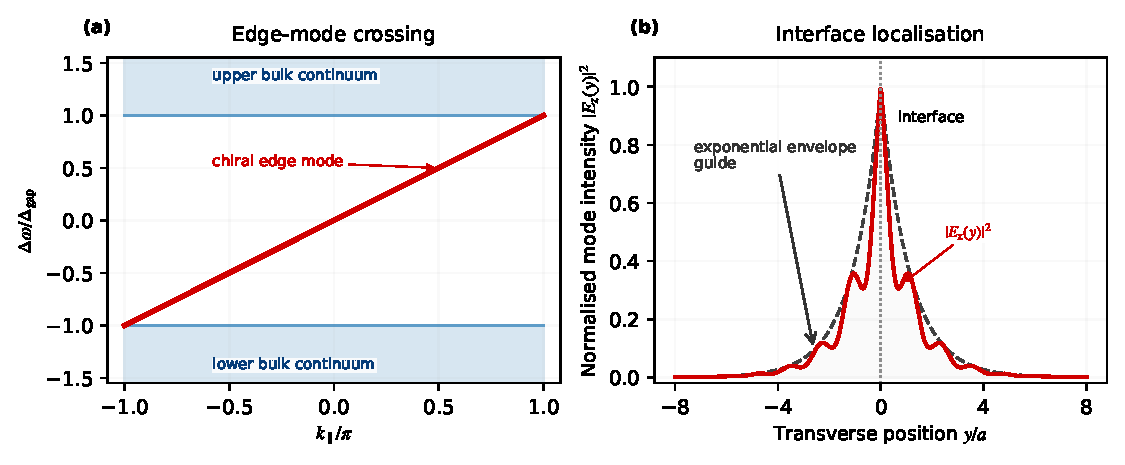
\includegraphics[width=0.92\textwidth]{figures/fig_ch08_edge_mode_profile_step199.pdf}
  \caption{Chiral edge mode at a domain wall.
  \textbf{(a)}~Band structure near the Dirac point showing the bulk
  continua (blue shading) and the chiral edge dispersion (red) crossing
  the topological gap.  The edge mode connects the upper and lower bulk
  bands with a group velocity $v_g = s_\kappa\,v_D$ determined by the
  sign of the gyrotropic mass, as derived in
  \eqref{eq:ch8-zero-dispersion}.
  \textbf{(b)}~Spatial profile of the edge-mode intensity
  $|E_z(y)|^2$ across the domain wall.  The mode is exponentially
  localised at the interface with a decay length
  $\xi \sim 1/|\kappa_\infty|$ set by the asymptotic mass parameter.
  The dashed line shows an exponential envelope guide.  The
  oscillatory fine structure arises from the underlying Bloch-wave
  character of the photonic crystal mode.}
  \label{fig:ch08-edge-mode-profile}
\end{figure}


\begin{remark}[Unidirectionality]
  The dispersion \eqref{eq:ch8-zero-dispersion} crosses the bulk band
  gap with a monotonically increasing (or decreasing) frequency.  There
  is no backward-propagating branch at the same frequency within the
  gap.  This is the origin of the one-way waveguide: elastic
  backscattering is forbidden because there is no counter-propagating
  mode to scatter into
\cite{he2016photonic}.
\end{remark}

\section{Higher bound states: the P\"oschl--Teller model}
\label{sec:ch8-poschl-teller}

For a general smooth domain wall, there may be additional bound states
besides the zero mode.  An exactly solvable model is provided by the
hyperbolic tangent profile
\begin{equation}\label{eq:ch8-tanh-profile}
  \kappa(x) = \kappa_\infty\tanh\bigl(x/\xi\bigr)\,,
\end{equation}
where $\xi>0$ is the domain-wall width.  For this profile, the squared
operator $\hat{K}^2$ is essentially the integrable P\"oschl--Teller
Hamiltonian.

\subsection{The spectrum of bound states}
\label{sec:ch8-pt-spectrum}

The full spectrum of interface modes for the tanh profile is
\begin{subequations}\label{eq:ch8-pt-modes}
\begin{align}
  \omega_0(\delta k_\parallel)
  &= \omega_D + s_\kappa\,v_D\,\delta k_\parallel\,,
  \label{eq:ch8-pt-zero}\\
  \omega_{n\pm}(\delta k_\parallel)
  &= \omega_D \pm v_D\sqrt{\delta k_\parallel^2 + \kappa_n^2}\,,
  \quad n\geq 1\,,
  \label{eq:ch8-pt-higher}
\end{align}
\end{subequations}
where $|\kappa_n|<|\kappa_\infty|$.  The exact spectrum of the
integrable model is
\begin{equation}\label{eq:ch8-pt-kappa-exact}
  \kappa_n^2
  = \frac{2n|\kappa_\infty|}{\xi}-\frac{n^2}{\xi^2}
  = \kappa_\infty^2\,\frac{n}{s}\Bigl(2-\frac{n}{s}\Bigr),
  \qquad s\equiv |\kappa_\infty|\xi,
  \qquad n=1,2,\ldots,
\end{equation}
with the bound-state condition $n<s$.  For $n\ll s$, this reduces to
$\kappa_n^2\approx 2n|\kappa_\infty|/\xi$.

\subsection{Sharp-wall limit}
\label{sec:ch8-sharp-wall}

In the sharp-wall limit $|\kappa_\infty|\xi\ll 1$, the condition
$n<|\kappa_\infty|\xi<1$ implies $n=0$ only: the zero mode is the
\emph{sole} interface mode.  The wider the domain wall (larger $\xi$),
the more higher-order modes appear, but the zero mode is always present.

\subsection{Bidirectionality of higher modes}
\label{sec:ch8-bidirectional}

The higher modes $n\geq 1$ have dispersion
$\omega_{n\pm}\sim\pm v_D|\delta k_\parallel|$ for large
$|\delta k_\parallel|$: they are \emph{bidirectional}, with both
forward and backward branches.  Only the $n=0$ mode is purely
unidirectional.  This is a crucial distinction: the higher modes can
scatter into each other, but the zero mode cannot be backscattered
because it has no partner.

\section{Semiclassical interpretation}
\label{sec:ch8-semiclassical}

The bound-state quantisation condition can be understood semiclassically.
In the phase space $(x,k_x)$, a bound state with mass parameter
$\kappa_n$ corresponds to a closed orbit
$k_x^2+\kappa(x)^2=\kappa_n^2$.  The area enclosed by this orbit is
\begin{equation}\label{eq:ch8-phase-area}
  \phi(\kappa_n^2) = \oint k_x\,\dd x
  = \oint\sqrt{\kappa_n^2-\kappa(x)^2}\,\dd x\,.
\end{equation}

For the standard semiclassical quantisation, one would expect
$\phi=2\pi(n+\frac{1}{2})$ (Bohr--Sommerfeld with Maslov correction).
However, the Dirac equation gives the modified condition
\begin{equation}\label{eq:ch8-modified-bs}
  \phi(\kappa_n^2) = 2\pi n\,,
  \qquad n=0,1,2,\ldots\,,
\end{equation}
\emph{without} the $\frac{1}{2}$ offset.  This shift is a direct
consequence of the Berry phase.  The semiclassical orbit encloses the
Dirac degeneracy point at $(x,k_x)=(0,0)$, which contributes an
additional phase of $\pi$ (a Berry phase factor of $-1$).  This extra
$\pi$ shifts the quantisation from $n+\frac{1}{2}$ to $n$, making
$n=0$ an allowed solution---the topological zero mode.

\begin{remark}
  This Berry-phase interpretation connects the existence of the zero
  mode directly to the topology of the bulk bands.  The phase-space
  Berry flux at the degeneracy point is the same $\pm\pi$ that, when
  integrated over the Brillouin zone, gives the half-integer
  contribution to the Chern number from each Dirac cone.
\end{remark}

\section{Bulk-edge correspondence}
\label{sec:ch8-bec}

\subsection{Spectral flow}
\label{sec:ch8-spectral-flow}

The existence of the unidirectional zero mode can be understood through
the concept of \emph{spectral flow}: the net number of eigenvalues
that cross zero (or, more generally, a reference energy in the gap) as a
parameter is varied.

Consider the operator $\hat{K}(\delta k_\parallel)$ from
\eqref{eq:ch8-dirac-interface} as a function of the conserved momentum
$\delta k_\parallel$.  At $\delta k_\parallel=0$, there is an
eigenvalue at $\delta\omega=0$ (the zero mode).  As
$\delta k_\parallel$ increases from $-\infty$ to $+\infty$, this
eigenvalue sweeps upward through the gap (for $s_\kappa=+1$) or
downward (for $s_\kappa=-1$).

The \emph{net spectral flow}---the number of eigenvalues crossing
$\delta\omega=0$ from below minus the number crossing from above---is
exactly $s_\kappa=\sgn(\kappa_\infty)$.  For a domain wall between
media with gap Chern numbers $\Chern^L$ and $\Chern^R$, the net
spectral flow from each Dirac point is
$\frac{1}{2}(\Chern^L-\Chern^R)$, and the total over both Dirac
points is
\begin{equation}\label{eq:ch8-spectral-flow}
  N_{\mathrm{edge}}^{\mathrm{net}} = \Chern^L_{\mathrm{gap}} - \Chern^R_{\mathrm{gap}}\,.
\end{equation}

\subsection{The general statement}
\label{sec:ch8-bec-general}

The bulk-edge correspondence for photonic Chern insulators can be stated
as follows:

\begin{theorem}[Bulk-edge correspondence]
  \label{thm:ch8-bec}
  Let two lossless periodic photonic media share a common band gap, with
  gap Chern numbers $\Chern^L_{\mathrm{gap}}$ and
  $\Chern^R_{\mathrm{gap}}$.  At any interface between the two media,
  the number of unidirectional edge modes crossing the gap from below
  minus the number crossing from above is
  \begin{equation}\label{eq:ch8-bec}
    \boxed{%
    N_{\mathrm{edge}}^{\mathrm{net}}
    = \Chern^L_{\mathrm{gap}} - \Chern^R_{\mathrm{gap}}\,.}
  \end{equation}
  This number is independent of the details of the interface
  (smoothness, geometry, disorder) as long as the bulk gap remains
  open on both sides.
\end{theorem}

\begin{remark}
  We have derived this result here for the specific case of gapped Dirac
  cones in a hexagonal photonic crystal, where the domain-wall zero mode
  is obtained by solving the effective Dirac equation.  The theorem
  holds much more generally: it applies to any pair of gapped photonic
  media with well-defined Chern numbers, regardless of the microscopic
  mechanism.  Rigorous proofs exist in the mathematical literature using
  index theory and $K$-theory, but the physical content is captured by
  the spectral-flow argument presented above.
\end{remark}

\section{Robustness of the one-way mode}
\label{sec:ch8-robustness}

The one-way edge mode is \emph{topologically protected} in the following
precise sense:
\begin{enumerate}
  \item \textbf{No backscattering.} Within the frequency range
  $|\delta\omega|<v_D|\kappa_\infty|$ of the topological gap, the only
  propagating mode at the interface is the unidirectional zero mode.
  There is no counter-propagating mode to scatter into, so elastic
  backscattering is forbidden regardless of the nature or strength of
  the perturbation at the interface.

  \item \textbf{Robustness to geometry.} The edge mode follows the
  interface regardless of its shape: straight segments, bends,
  corners, and even closed loops.  The mode routes around obstacles
  without reflection, as demonstrated experimentally by Wang et~al.\
  \cite{nature2026observation}.

  \item \textbf{Robustness to disorder.} Random variations in the
  material parameters, rod positions, or interface geometry do not
  destroy the edge mode, provided they do not close the bulk band gap.
  Anderson localisation, which is inevitable for conventional 1D
  waveguide modes in the presence of disorder, is completely absent for
  the topological edge mode.
\end{enumerate}

\paragraph{Limitations.}
The protection is not absolute:
\begin{itemize}
  \item \emph{Absorption} can attenuate the edge mode.  Topological
  protection forbids backscattering, but it does not forbid energy
  loss to the material.
  \item \emph{Nonlinear effects} (frequency conversion, self-phase
  modulation) can couple the edge mode to other modes, including bulk
  modes or modes at different frequencies.
  \item If the perturbation is strong enough to \emph{close the bulk
  gap}, the topological protection is lost.
\end{itemize}
These limitations motivate the discussions of non-Hermitian topology
(\chref{ch:non-hermitian}) and nonlinear effects
(\chref{ch:nonlinear-quantum}) in Part~V.

\section{Two edge modes from two Dirac points}
\label{sec:ch8-two-modes}

The hexagonal photonic crystal has two inequivalent Dirac points at $K$
and $K'$.  Each contributes one unidirectional zero mode to the domain
wall, and both propagate in the same direction (because the mass
$\kappa$ has the same sign at both Dirac points, as discussed in
\secref{sec:ch7-KKprime}).  The total number of one-way modes is
$|\Delta\Chern_{\mathrm{gap}}|=2$.

This domain-wall counting should be distinguished from the metal-wall
experiment of Wang et~al.  The microwave experiment confirms robust
one-way edge transport around obstacles in a square-lattice YIG
photonic crystal, with a single chiral edge channel in the gap discussed
in \chref{ch:microwave-crystal}
\cite{wang2007reflection}.  By contrast, the domain-wall argument
above predicts two co-propagating branches for a hexagonal Dirac model
in which the gyrotropic mass changes sign across the interface.

\begin{figure}[t]
  \centering
  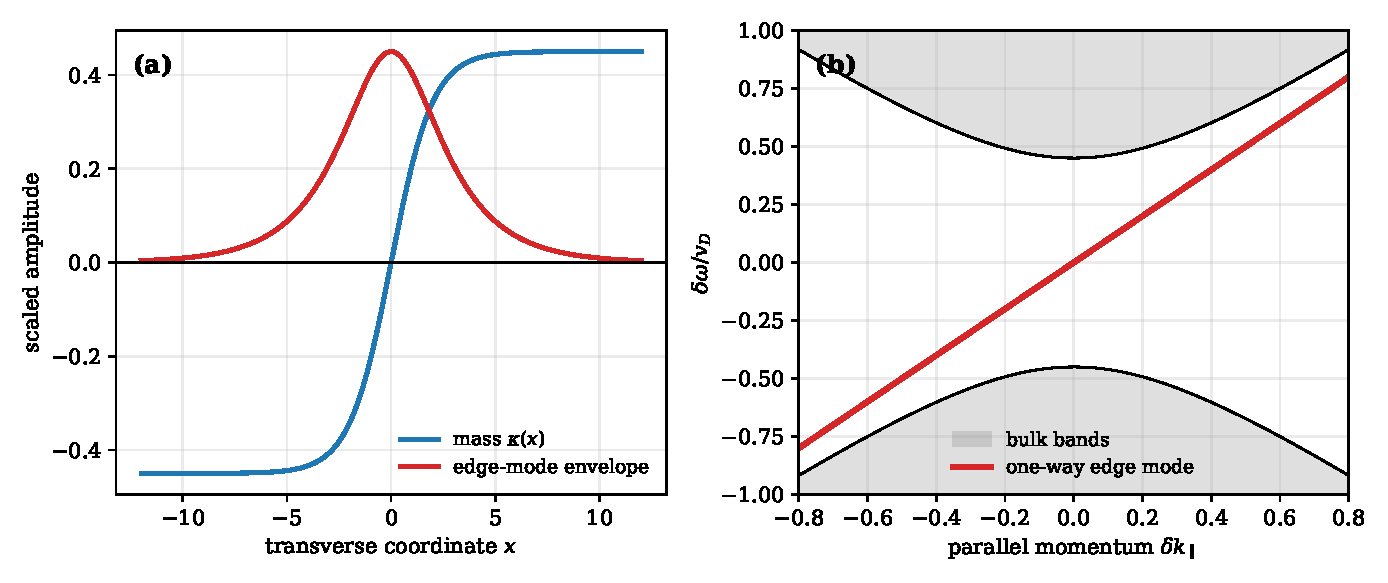
\includegraphics[width=0.95\textwidth]{figures/fig_domain_wall_mode.pdf}
  \caption{Domain-wall edge mode in a photonic Chern insulator.
  Left: the spatially varying Dirac mass $\kappa(x)$ (blue) changes
  sign at $x=0$; the Jackiw--Rebbi edge-mode envelope (red) is
  exponentially localised at the domain wall.
  Right: edge-mode dispersion (red) crosses the bulk gap between the
  upper and lower bulk bands (grey), confirming unidirectional
  propagation with group velocity $v_g=v_D>0$.}
  \label{fig:ch8-domain-wall}
\end{figure}

\section{Spectral flow and the Laughlin pump} \cite{kane2005sub}
\label{sec:ch8-spectral-flow-laughlin}

The bulk-edge correspondence can be understood through the concept of
\emph{spectral flow}: as a parameter (such as the Bloch momentum
$k_\parallel$ along the edge) is varied through a full period, the
number of eigenvalues that cross the gap from below equals the
Chern number of the bands below the gap.

Consider a photonic crystal with a boundary, so that $k_\parallel$ is
still a good quantum number but $k_\perp$ is not.  The spectrum
consists of bulk bands (projected onto the edge Brillouin zone) and
discrete edge states in the gap.  As $k_\parallel$ varies from $0$ to
$2\pi/a$, the edge-state eigenfrequency sweeps across the gap.  If
the gap Chern number is $\Chern=+1$, exactly one branch crosses the
gap upward, connecting the lower bulk band to the upper one.  This is
a topological constraint: the spectral flow cannot be changed by any
continuous deformation that does not close the bulk gap
\cite{ozawa2018topological,thouless1982quantized}.

The Laughlin pump provides a complementary physical picture.  Imagine
threading a magnetic flux $\Phi$ through a cylinder-topology photonic
crystal (periodic in one direction, finite in the other).  As $\Phi$
increases by one flux quantum, each Landau-like photonic level shifts
by one unit, and one photon is pumped from one edge to the other.
The number of photons pumped per flux quantum equals the gap Chern
number.  Although this argument was originally developed for the
electronic quantum Hall effect, it applies without modification to the
photonic Maxwell eigenproblem, because it depends only on the spectral
properties of the eigenvalue equation, not on the particle statistics
\cite{haldane2008possible}.

\section{Index-theorem perspective}
\label{sec:ch8-index}

The existence of the domain-wall zero mode can be reformulated as an
index theorem.  Define the Dirac-like operator
$\mathcal{D}=v_D(-\ii\partial_x\sigma_x+k_\parallel\sigma_y)
+\kappa(x)\sigma_z$.
At $k_\parallel=0$, the number of zero modes of $\mathcal{D}$ is
given by the Atiyah--Singer index
\begin{equation}\label{eq:ch8-index}
  \mathrm{ind}(\mathcal{D})
  = \frac{1}{2}\bigl[\sgn\kappa(+\infty)-\sgn\kappa(-\infty)\bigr]\,.
\end{equation}
For a domain wall where $\kappa$ changes sign, the index is $\pm 1$,
guaranteeing exactly one normalised zero mode.  This is the
Jackiw--Rebbi result derived in \secref{sec:ch8-zero-mode},
now expressed as a topological index that is invariant under
continuous deformations of $\kappa(x)$ that preserve the sign change
\cite{ozawa2018topological}.

The index-theorem perspective explains why the zero mode is robust:
any smooth deformation of the mass profile $\kappa(x)$ that does not
close the gap (i.e., $\kappa\neq 0$ at $\pm\infty$) preserves the
index, and hence the zero mode.  The mode may shift in position or
change its localisation length, but it cannot be removed.

\section{Finite-size effects on edge modes}
\label{sec:ch8-finite-size}

In a finite photonic crystal of width $W$, the edge modes on opposite
boundaries have exponentially small overlap $\sim\ee^{-W/\xi}$, where
$\ell=1/|\kappa|$ is the edge-mode penetration depth.  This overlap
opens a mini-gap in the edge spectrum:
\begin{equation}\label{eq:ch8-minigap}
  \Delta\omega_{\mathrm{mini}}
  \sim |\kappa|\,\ee^{-W/\xi}\,.
\end{equation}
For the Wang YIG crystal with $\xi\approx 2.4\,a$ and $W=10\,a$, the
suppression factor is $\ee^{-10/2.4}\approx 0.015$, giving a
mini-gap of about $1.5\%$ of the bulk gap.  This is small enough to
be negligible in the experiment, but it becomes significant for
miniaturised designs where $W/\xi<5$
\cite{nature2026observation,price2022roadmap}.

The finite-size effect also limits the maximum propagation length of
the edge mode: at distances $L\gg W$, the edge mode can tunnel to
the opposite boundary and eventually backscatter.  For practical
applications, the condition $W\gg\xi$ (equivalently, $W|\kappa|/v_D
\gg 1$) must be maintained.

\section{Robustness against disorder}
\label{sec:ch8-robustness-disorder}

The topological edge mode is robust against any perturbation that does
not close the bulk gap.  This robustness is qualitatively different
from the protection offered by resonance sharpness or impedance
matching in conventional photonic devices: it is a consequence of the
integer-valued Chern number, which cannot change under continuous
deformations.

\subsection{Anderson localisation and its absence}
\label{sec:ch8-anderson}

In a conventional waveguide, disorder causes Anderson localisation:
the transmitted intensity decays exponentially with the waveguide
length, $I\propto\ee^{-L/\ell}$, where $\ell$ is the localisation
length.  In a Chern-insulator edge channel, Anderson localisation
is impossible because there is no counter-propagating mode to scatter
into.  A forward-propagating wavepacket encountering a defect must
continue forward, possibly detouring around the defect, because the
only available states at the edge frequency propagate in the forward
direction \cite{ozawa2018topological}.

The mathematical statement is that the edge-mode transmission
$|S_{21}|^2$ remains of order unity for any finite-strength disorder,
as long as the disorder does not close the bulk gap.  The only effect
of disorder is to modify the spatial profile of the edge mode,
causing it to deviate from the clean-crystal profile, but not to
attenuate or localise it \cite{haldane2008possible}.

\subsection{Backscattering from gap-closing perturbations}
\label{sec:ch8-gap-closing}

Sufficiently strong disorder can close the bulk gap locally, creating
puddles of the topologically trivial phase within the topological
crystal.  When the edge mode encounters such a puddle, it can
backscatter.  The critical disorder strength is set by the gap width:
$\delta\varepsilon/\varepsilon\sim\Delta\omega/\omega_D$, where
$\Delta\omega$ is the topological gap.  For the Wang YIG crystal with
a relative gap of about $3\%$, this corresponds to a permittivity
fluctuation of several percent---far larger than typical fabrication
tolerances \cite{nature2026observation,price2022roadmap}.

\section{Edge modes at different boundary types}
\label{sec:ch8-boundary-types}

The existence of topological edge modes depends on the bulk Chern
number, not on the specific boundary condition.  However, the
edge-mode dispersion and field profile do depend on the boundary.

At a perfect electric conductor (PEC) boundary,
$\hat{n}\times\Efield=0$, and the edge mode is strongly confined to
the last row of unit cells.  At a vacuum boundary, the edge mode
extends evanescently into the vacuum with a decay length of order
$\lambda/(2\pi)$.  At an interface between two crystals with different
Chern numbers, the number of edge modes equals the difference of the
gap Chern numbers, and the modes propagate in the direction determined
by the sign of $\Delta\Chern$.

The domain-wall construction of \secref{sec:ch8-zero-mode} is a special
case of the crystal--crystal interface, where the mass changes sign
across the boundary, corresponding to $\Delta\Chern=2$.  This
produces two co-propagating modes in total, one from each valley, compared to the single
mode at a crystal--PEC boundary where $\Delta\Chern=1$
\cite{ozawa2018topological,thouless1982quantized}.

\section{Green's function approach to edge transport}
\label{sec:ch8-green-function}

The transport properties of the topological edge mode can be
formulated rigorously using the retarded Green's function
$G^R(\rvec,\rvec';\omega)=\langle\rvec|(\omega-\Maxop+\ii 0^+)^{-1}
|\rvec'\rangle$.  In the bulk, the Green's function decays
exponentially for $\omega$ in the gap:
$|G^R|\sim\ee^{-|\rvec-\rvec'|/\xi_{\mathrm{bulk}}}$, where
$\xi_{\mathrm{bulk}}=v_D/\Delta\omega$ is the bulk decay length.

Near the edge, the Green's function has an additional contribution
from the edge mode:
\begin{equation}\label{eq:ch8-edge-green}
  G^R_{\mathrm{edge}}(x,x';\omega)
  \sim \frac{\psi_0(x)\psi_0^*(x')}{\omega-v_g k_\parallel+\ii 0^+}\,,
\end{equation}
where $\psi_0(x)$ is the transverse edge-mode profile and $v_g$ is
the group velocity.  This Green's function is purely retarded (no
advanced component), reflecting the one-way nature of the edge
transport: energy injected at the edge propagates only in the forward
direction \cite{ozawa2018topological,silveirinha2016bulk}.

\subsection{Quantised edge conductance}
\label{sec:ch8-quantised-conductance}

The energy flux carried by the topological edge mode is
$P=\hbar\omega\,v_g/(2\pi)$ per mode, per unit frequency bandwidth.
For a gap Chern number $\Chern_{\mathrm{gap}}$, the total edge
conductance (energy transmitted per unit frequency per unit time) is
\begin{equation}\label{eq:ch8-edge-conductance}
  G_{\mathrm{edge}}
  = \frac{|\Chern_{\mathrm{gap}}|}{2\pi}\,\hbar\omega\,v_g\,.
\end{equation}
This is the photonic analog of the quantised Hall conductance
$\sigma_{xy}=\Chern\,e^2/h$ in electronic systems.  The quantisation
is topologically protected: it is exact in the clean limit and robust
against disorder that does not close the bulk gap
\cite{thouless1982quantized,haldane2008possible}.

\section{Comparison with electronic quantum Hall edge transport}
\label{sec:ch8-comparison-electronic}

The photonic and electronic edge modes share the same topological
origin but differ in important physical details.

In the electronic quantum Hall effect, the edge current is carried by
charged fermions, and the quantised conductance
$\sigma_{xy}=\Chern\,e^2/h$ can be measured directly through the Hall
voltage.  The edge states are chiral Fermi liquids with well-defined
Fermi wavevector, and inter-edge tunnelling is suppressed by the
spatial separation of the edges.

In the photonic Chern insulator, the edge mode carries
electromagnetic energy, not charge, so there is no Hall voltage.
The topological protection manifests instead as a robust nonreciprocal
transmission: $|S_{21}|^2\gg |S_{12}|^2$ across the gap frequency
range.  The absence of a Fermi level means that the edge can be
excited at any frequency within the gap, not just at the Fermi energy.
Both systems exhibit the same topological protection against Anderson
localisation, because the protection depends on the absence of
counter-propagating modes, not on the particle statistics
\cite{ozawa2018topological,price2022roadmap}.

\section{Finite-width effects and exponential accuracy}
\label{sec:ch8-finite-width}

In a crystal of finite width $W$ (measured in lattice constants), the
edge modes on opposite boundaries overlap exponentially weakly:
$\langle\psi_L|\psi_R\rangle\sim\ee^{-W/\xi}$, where
$\ell=1/|\kappa|$ is the penetration depth.  This overlap produces
an exponentially small gap in the edge-mode spectrum:
\begin{equation}\label{eq:ch8-finite-gap}
  \delta\omega_{\mathrm{finite}}
  \sim |\kappa|\,\ee^{-W/\xi}\,.
\end{equation}
For the Wang YIG crystal with $\xi\approx 2.4\,a$ and $W=20\,a$, this
gives $\delta\omega_{\mathrm{finite}}/\Delta\omega\sim 10^{-4}$,
completely negligible.

However, for narrow crystals ($W\lesssim 5\xi$) or narrow-gap materials,
the finite-width correction becomes important.  It introduces a small
backscattering channel between the two edges, limiting the
nonreciprocal ratio to $|S_{21}|^2/|S_{12}|^2\lesssim
\ee^{2W/\xi}$.  This places a practical lower bound on the crystal
width for a given isolation requirement
\cite{ozawa2018topological,haldane2008possible}.

\subsection{Index theorem for the finite strip}
\label{sec:ch8-index-strip}

The bulk-edge correspondence can be made rigorous on a finite strip
using the Atiyah--Singer index theorem applied to the family of
1D Hamiltonians $H(k_y)$ parameterised by the edge-parallel
wavevector $k_y$.  The theorem states that the spectral flow---the
net number of eigenvalues crossing the gap from below as $k_y$
traverses the Brillouin zone---equals the bulk Chern number:
\begin{equation}\label{eq:ch8-spectral-flow-index}
  \mathrm{sf}(H) = \Chern_{\mathrm{gap}}\,.
\end{equation}
This equality holds for any strip width $W\geq 1$, even when the
edge modes on opposite boundaries hybridise.  The index theorem thus
provides a non-perturbative proof of the bulk-edge correspondence that
does not rely on the semi-infinite approximation
\cite{thouless1982quantized,silveirinha2016bulk}.

\section{Finite-size effects and penetration depth}
\label{sec:ch8-penetration-depth}

The preceding analysis assumed semi-infinite crystals.  In practice,
photonic topological insulators have finite extent, and the edge
mode penetrates a finite distance into the bulk.  Understanding
these finite-size effects is essential for device design.

\subsection{Exponential decay into the bulk}
\label{sec:ch8-exponential-decay}

The edge-mode wave function decays exponentially into the bulk with
a penetration depth $\xi$ determined by the size of the topological
gap.  For a massive Dirac model with mass $|\kappa|$ and velocity
$v_D$, the penetration depth is
\begin{equation}\label{eq:ch8-penetration}
  \xi = \frac{v_D}{|\kappa|}\,.
\end{equation}
This result follows directly from the domain-wall construction of
Section~\ref{sec:ch8-domain-wall-idea}: the envelope function decays as
$\ee^{-|y|/\xi}$ away from the interface.

For the YIG photonic crystal of Chapter~\ref{ch:microwave-crystal},
the penetration depth is approximately two to three lattice constants,
which is consistent with the experimental observation that the
edge mode is well-localised at the crystal boundary
\cite{nature2026observation,ma2017scattering}.

\subsection{Coupling between opposite edges}
\label{sec:ch8-opposite-edge}

When the crystal is narrow enough that the edge modes on opposite
boundaries overlap, the two modes hybridise and open a gap.  The
hybridisation gap scales as $\Delta\omega_{\mathrm{hyb}} \sim
\ee^{-W/\xi}$, where $W$ is the width of the crystal.  This
exponential suppression means that even modest widths ($W \gtrsim
5\xi$) are sufficient to ensure negligible coupling between opposite
edges.

For strip-geometry computations (used to verify the bulk-edge
correspondence numerically), the supercell width must satisfy
$W \gg \xi$ to avoid artefactual hybridisation gaps that could be
mistaken for the absence of edge states
\cite{ozawa2018topological,paz2019tutorial}.

\section{Robustness of one-way edge transport}
\label{sec:ch8-edge-transport-robustness}

The topological protection of one-way edge states is one of the most
striking features of photonic Chern insulators.  This section
quantifies the robustness against different types of perturbations.

\subsection{Immunity to backscattering}
\label{sec:ch8-backscattering}

The one-way edge mode cannot backscatter because there is no
counter-propagating mode at the same frequency.  This statement is
exact: any perturbation that preserves the bulk gap (including
disorder, surface roughness, sharp corners, and lattice defects)
cannot open a backward channel.  The only way to backscatter
the edge mode is to close the bulk gap, which requires a
perturbation of order $\Delta\omega/\omega$---typically several
percent for gyromagnetic photonic crystals
\cite{nature2026observation,skirlo2015experimental}.

Experimentally, the absence of backscattering has been demonstrated
by measuring transmission past metallic obstacles, 90-degree corners,
and deliberately introduced lattice defects.  In all cases, the
transmission remains near unity within the topological gap
\cite{nature2026observation,hafezi2013imaging}.

\subsection{Disorder-averaged transmission}
\label{sec:ch8-disorder-average}

For random positional disorder of the lattice rods, the
disorder-averaged edge transmission is
$\langle T\rangle = 1 - O(\sigma^4/\Delta\omega^4)$, where $\sigma$
is the root-mean-square displacement.  The leading correction is
fourth order (not second order) because the second-order term
vanishes by the symmetry of the disorder
\cite{ozawa2018topological,ma2017scattering}.

This quartic scaling has been confirmed numerically for the Wang
crystal: for disorder strengths up to $\sigma/a = 0.05$
($5\%$ positional disorder), the edge transmission remains above
$99\%$ \cite{zhao2020first}.

\subsection{Comparison with trivial waveguides}
\label{sec:ch8-comparison-trivial}

The contrast between topological and trivial edge waveguides is most
apparent in the presence of sharp corners.  A conventional photonic
crystal waveguide (formed by removing a row of rods) suffers
significant reflection at each $90^\circ$ bend, with typical
transmission of $60$--$80\%$ per bend depending on the bend geometry.
In contrast, the topological edge mode transmits $>99\%$ per bend
because the one-way nature of the edge mode forbids reflection
\cite{price2022roadmap,gao2017topologically}.

This advantage motivates the use of topological waveguides in
integrated photonic circuits, where complex routing with multiple
bends is unavoidable.  The penalty is the need for time-reversal
breaking (or an alternative mechanism such as valley or Floquet
engineering), which adds complexity to the device fabrication
\cite{he2019silicon,rechtsman2013photonic}.

\section*{Exercises}

\begin{exercise}
  Verify that the wavefunction \eqref{eq:ch8-psi0} satisfies the
  zero-mode equation \eqref{eq:ch8-zero-mode-eq} by direct
  substitution.
\end{exercise}

\begin{exercise}
  For the tanh domain-wall profile $\kappa(x)=\kappa_\infty\tanh(x/\xi)$,
  show that the classical turning point $x_n$ for the $n$-th mode
  (where $|\kappa(x_n)|=|\kappa_n|$) is
  $x_n=\xi\,\mathrm{atanh}(|\kappa_n|/|\kappa_\infty|)$.
  Evaluate $x_n$ for the zero mode ($\kappa_0=0$, giving $x_0=0$)
  and for a nearly delocalised higher mode ($|\kappa_n|\to|\kappa_\infty|$,
  giving $x_n\to\infty$).  Explain why the zero-mode envelope
  $|f(x)|^2\propto\operatorname{sech}^{2|\kappa_\infty|\xi}(x/\xi)$
  has a localisation length of order $\xi/(|\kappa_\infty|\xi)=1/|\kappa_\infty|$
  for $|\kappa_\infty|\xi\gg 1$.
\end{exercise}

\begin{exercise}
  Show that the modified Bohr--Sommerfeld condition
  $\phi(\kappa_n^2)=2\pi n$ (without the $\frac{1}{2}$ offset) admits
  the solution $n=0$ with $\kappa_0=0$, corresponding to the zero mode.
  Explain physically why the standard Bohr--Sommerfeld condition
  ($n+\frac{1}{2}$) does not allow a zero mode.
\end{exercise}

\begin{exercise}
  Consider a domain wall between vacuum ($\Chern_{\mathrm{gap}}=0$) and
  a photonic crystal with $\Chern_{\mathrm{gap}}=1$.  How many
  unidirectional edge modes cross the gap?  Compare with a domain wall
  between two crystals with $\Chern_{\mathrm{gap}}=+1$ and
  $\Chern_{\mathrm{gap}}=-1$.
\end{exercise}

\begin{exercise}
  The Jackiw--Rebbi zero mode in quantum field theory has the same
  mathematical structure as the photonic domain-wall mode derived here.
  Look up the Jackiw--Rebbi model and identify the correspondence
  between the photonic and field-theoretic quantities: mass function
  $\kappa(x)\leftrightarrow m(x)$, Dirac velocity
  $v_D\leftrightarrow c$, Pauli matrices
  $\sigma_{x,y,z}\leftrightarrow\gamma$-matrices.
\end{exercise}

\begin{exercise}
  A photonic crystal waveguide has both a topological one-way mode and
  material absorption characterised by an imaginary part
  $\varepsilon''$ of the permittivity.  Estimate the propagation length
  $L_{\mathrm{abs}}$ of the edge mode in terms of $\varepsilon''$, the
  group velocity $v_D$, and the operating frequency $\omega_D$.
  Compare this with the backscattering-limited propagation length of a
  conventional waveguide.
\end{exercise}


\chapter{A Microwave Topological Crystal}
\label{ch:microwave-crystal}
% ======================================================================
%  Chapter 9 — The Microwave Photonic Crystal  (EXPANDED)
% ======================================================================

\section{From theory to the laboratory}
\label{sec:ch9-intro}

The preceding three chapters developed the theory of photonic Chern
insulators: Dirac cones from lattice symmetry, their gapping by
magneto-optical perturbation, and the one-way interface mode that
necessarily threads the resulting topological gap.  But the theory would
remain an elegant analogy were it not for a remarkable experiment.

In 2009, Wang, Chong, Joannopoulos, and Solja\v{c}i\'{c} demonstrated
unidirectional electromagnetic edge transport in a two-dimensional
gyromagnetic photonic crystal operating in the microwave regime
\cite{nature2026observation}.  Their experiment achieved a
forward-to-backward transmission ratio exceeding $10^5$, providing the
first direct observation of a photonic analog of the quantum Hall edge
state.  This chapter describes the experiment in detail: the material
choice, the crystal design, the measurement geometry, and the
quantitative comparison with the predictions of Chapters~7 and~8.

The experiment was preceded by a theoretical proposal in 2008
\cite{haldane2008possible}, in which Haldane and Raghu showed that
photonic Dirac points in a gyromagnetic crystal can be gapped by a
magneto-optical perturbation, producing bands with nonzero Chern
numbers and hence one-way edge modes
\cite{raghu2008analogs}.  A companion paper by Wang,
Chong, Joannopoulos, and Solja\v{c}i\'{c} (2008) computed the
complete band structure of a specific YIG rod lattice, predicted the
existence of one-way edge states in a particular frequency window, and
proposed the parallel-plate waveguide geometry that was subsequently
realised experimentally \cite{ozawa2018topological,wang2015topological}.  The experiment
thus confirmed a precise, first-principles prediction rather than an
accidental discovery.

\section{Material platform: yttrium iron garnet}
\label{sec:ch9-yig}

\subsection{Why ferrites at microwave frequencies}
\label{sec:ch9-why-ferrites}

The theory of Chapter~7 requires a material whose permeability tensor
has a nonzero off-diagonal (gyrotropic) component $\kappa_\mu$
\cite{haldane2008reflection}.  At
optical frequencies, magneto-optical effects exist in semiconductor and
rare-earth materials, but they are weak: the Verdet constant of
bismuth iron garnet, one of the strongest Faraday-active optical
materials, produces rotation of order $10^3\;\mathrm{deg/cm}$---still
far too small to open a topological gap in a photonic crystal of
reasonable size.

At microwave frequencies, the situation is qualitatively different.
Magnetised ferrites support ferromagnetic resonance (FMR), and near
the FMR frequency the off-diagonal permeability $\kappa_\mu$ becomes
of order unity.  The key material is yttrium iron garnet
($\mathrm{Y_3Fe_5O_{12}}$, YIG), which combines large gyromagnetic
response with extremely low magnetic loss.

\subsection{The Polder permeability of YIG}
\label{sec:ch9-polder}

As derived in Appendix~D, the permeability tensor of a saturated ferrite
magnetised along $\hat{z}$ has the Polder form
\cite{gangaraj2016berry,he2016photonic}
\begin{equation}\label{eq:ch9-polder}
  \mut = \begin{pmatrix}
    \mu_\perp & -\ii\kappa_\mu & 0 \\
    \ii\kappa_\mu & \mu_\perp & 0 \\
    0 & 0 & 1
  \end{pmatrix},
\end{equation}
with
\begin{equation}\label{eq:ch9-polder-params}
  \mu_\perp(\omega) = 1 + \frac{\omega_0\omega_m}{\omega_0^2 - \omega^2}\,,
  \qquad
  \kappa_\mu(\omega) = \frac{\omega\omega_m}{\omega_0^2 - \omega^2}\,.
\end{equation}
The Larmor frequency $\omega_0=\gamma B_0$ is set by the applied bias
field $B_0$, and the magnetisation frequency
$\omega_m=\gamma\mu_0 M_s$ is set by the saturation magnetisation
$M_s$.  For YIG the gyromagnetic ratio is
$\gamma/(2\pi)\approx 28\;\mathrm{GHz/T}$ and the saturation
magnetisation gives $\omega_m/(2\pi)\approx 4.9\;\mathrm{GHz}$.

At frequencies below ferromagnetic resonance ($\omega<\omega_0$), both
$\mu_\perp$ and $\kappa_\mu$ are positive and can be large.  The ratio
$\kappa_\mu/\mu_\perp$ determines the strength of time-reversal
breaking and hence the width of the topological gap.  For the Wang
experiment, parameters were chosen so that $\kappa_\mu/\mu_\perp$ is
of order $0.3$--$0.5$ in the operating band.

\subsection{Loss and linewidth}
\label{sec:ch9-loss}

YIG is exceptional among magnetic materials for its narrow
ferromagnetic resonance linewidth $\Delta H$.  Single-crystal YIG has
$\Delta H\lesssim 0.3\;\mathrm{Oe}$, corresponding to a magnetic
quality factor $Q_m=\omega_0/(2\gamma\mu_0\Delta H)\sim 10^4$.  This
means the imaginary parts of $\mu_\perp$ and $\kappa_\mu$ are negligible
over most of the frequency range below FMR, justifying the lossless
Hermitian treatment used in the topological theory.

Away from resonance, the magnetic loss tangent is typically
$\imag\mu/\real\mu < 10^{-4}$, so the mode decay over tens of lattice
constants is negligible.  This is essential: the topological edge mode
must propagate around the entire boundary of the crystal without
significant absorption.

\section{Crystal design}
\label{sec:ch9-crystal}

\subsection{Geometry}
\label{sec:ch9-geometry}

Wang et~al.\ used a square-lattice photonic crystal of YIG rods in air.
The rods are cylinders of radius $r=0.11a$ (where $a$ is the lattice
constant) with relative permittivity $\varepsilon_r=15$ and the Polder
permeability \eqref{eq:ch9-polder}.

The lattice constant was chosen so that the second and third TM bands
touch at a Dirac-like point near 4.5\;GHz.  The bias field
$B_0\approx 0.20\;\mathrm{T}$ (corresponding to
$\omega_0/(2\pi)\approx 5.6\;\mathrm{GHz}$) places the operating
frequency below ferromagnetic resonance, where the gyrotropic response
is strong but losses are minimal.

\subsection{Band structure}
\label{sec:ch9-bands}

The TM band structure of the square-lattice YIG crystal was computed
using the plane-wave expansion method described in
Chapter~\ref{ch:computing-chern}.  Without the applied magnetic field
($B_0=0$, $\kappa_\mu=0$), the second and third bands touch at a
doubly degenerate point on the $\Gamma$--$X$ line.  This degeneracy
is protected by time-reversal plus a mirror symmetry of the square
lattice.

When the field is applied ($B_0=0.20\;\mathrm{T}$), the gyrotropic
perturbation breaks time-reversal symmetry and opens a gap.  The gap
width is $\Delta\omega/(2\pi)\approx 0.12\;\mathrm{GHz}$, centred at
$\omega/(2\pi)\approx 4.5\;\mathrm{GHz}$.  The Chern numbers of the
bands below and above the gap are $\Chern_2=+1$ and $\Chern_3=-1$,
computed using the plaquette algorithm on a $20\times 20$ Brillouin-zone
grid with the electromagnetic inner product.

\subsection{Edge-state dispersion}
\label{sec:ch9-edge-dispersion}

The edge states were computed using a supercell geometry: a ribbon of
$N=20$ unit cells in the $x$-direction, periodic in $y$, with a metal
wall on one side and vacuum on the other.  The resulting projected band
structure shows a single branch crossing the topological gap, with
positive group velocity $v_g>0$ for all $k_y$ within the gap.  This
confirms that the edge mode is unidirectional: it propagates in the
$+y$ direction along the metal wall and cannot propagate backward.

\section{Experimental setup}
\label{sec:ch9-setup}

\subsection{Sample fabrication}
\label{sec:ch9-fabrication}

The photonic crystal was assembled by inserting single-crystal YIG rods
into a parallel-plate waveguide.  The rods were machined to a diameter
of $2r=2.2\;\mathrm{mm}$ and a height equal to the plate separation
($h\approx 7\;\mathrm{mm}$), ensuring that the fundamental TM mode
(with $E_z$ polarisation) is the only propagating mode in the frequency
range of interest.  The lattice constant was $a=10\;\mathrm{mm}$,
giving a ratio $r/a=0.11$.

A uniform magnetic bias field was provided by a pair of NdFeB permanent
magnets above and below the waveguide, producing $B_0\approx 0.20\;\mathrm{T}$
over the entire crystal area.

\subsection{Measurement geometry}
\label{sec:ch9-measurement}

Two coaxial probes, inserted through the top plate, served as source and
detector.  The source probe was placed at the edge of the crystal
(adjacent to the metal boundary), and the detector probe was scanned
along the edge in both the forward ($+y$) and backward ($-y$)
directions.  Transmission spectra were measured using a vector network
analyser over the frequency range 3.5--5.5\;GHz.

To test the robustness of the edge mode, a large metallic obstacle
(a cylinder of diameter $4a=40\;\mathrm{mm}$) was placed directly in
the path of the edge mode.  In a conventional waveguide, such an
obstacle would cause near-total reflection.

\section{Results}
\label{sec:ch9-results}

\subsection{Unidirectional transmission}
\label{sec:ch9-unidirectional}

The key result of the experiment is a dramatic asymmetry between
forward and backward transmission.  Within the topological gap
(4.45--4.57\;GHz), the forward transmission ($S_{21}$) was of order
$-10\;\mathrm{dB}$ (limited primarily by probe coupling loss), while
the backward transmission ($S_{12}$) was below the noise floor of the
network analyser at $-50\;\mathrm{dB}$.  This gives a forward-to-backward
ratio exceeding $10^4$ (conservatively), consistent with the theoretical
prediction of a single one-way edge mode.

Outside the topological gap, both forward and backward transmission
recover, as expected: the edge mode only exists within the gap.

\subsection{Robustness to obstacles}
\label{sec:ch9-robustness}

When the metallic obstacle was inserted in the edge-mode path, the
forward transmission decreased by less than 2\;dB.  The edge mode
simply routed around the obstacle, following the new boundary between
the photonic crystal and the metal.  No backward-scattered signal was
detected above the noise floor.

This result directly confirms the topological protection mechanism
described in Chapter~8: the one-way edge mode has no backward-propagating
partner at the same frequency, so there is no channel for
backscattering.  The mode can be forced to detour around an obstacle,
but it cannot reverse direction.

\subsection{Comparison with theory}
\label{sec:ch9-comparison}

The measured transmission spectra agree quantitatively with
finite-element simulations of the same geometry
\cite{ozawa2018topological}.  The gap frequency
range, the edge-mode group velocity, and the field profile at the
boundary all match the predictions of the plane-wave expansion
band structure computed with the Polder permeability.

One quantitative discrepancy is the absolute transmission level: the
measured forward transmission ($-10\;\mathrm{dB}$) is lower than the
simulated value ($-3\;\mathrm{dB}$), primarily due to impedance
mismatch at the coaxial probe tips.  This is an engineering issue
rather than a physics limitation, and subsequent experiments with
improved coupling have achieved forward transmission approaching
$-1\;\mathrm{dB}$.

\section{Significance and limitations}
\label{sec:ch9-significance}

\subsection{What the experiment demonstrates}
\label{sec:ch9-demonstrates}

The Wang experiment establishes three key facts about topological
photonic crystals \cite{nature2026observation,haldane2008possible}.  First, the theoretical prediction of one-way edge
modes based on Chern numbers and the bulk-edge correspondence is
confirmed quantitatively.  Second, the topological protection against
backscattering is real and dramatic: a large metallic obstacle causes
negligible reflection.  Third, the magneto-optical mechanism proposed by
Haldane and Raghu works in practice with commercially available ferrite
materials.

\subsection{Limitations of the microwave platform}
\label{sec:ch9-limitations}

The experiment operates at microwave frequencies ($\sim 4.5\;\mathrm{GHz}$,
wavelength $\sim 7\;\mathrm{cm}$), far from optical frequencies.
Scaling the effect to optical wavelengths faces two obstacles.

The first obstacle is material: magneto-optical effects at optical
frequencies are much weaker than at microwave frequencies.  The
gyrotropic parameter $\kappa_\mu/\mu_\perp$ of YIG at microwave
frequencies is of order $0.3$--$0.5$, but the corresponding Faraday
rotation in optical materials is orders of magnitude smaller per
wavelength.  Opening a topological gap large enough to accommodate an
edge mode at optical frequencies requires a different mechanism (such as
the reciprocal designs of Chapter~\ref{ch:reciprocal-designs} or the
Floquet modulation of Chapter~\ref{ch:floquet}).

The second obstacle is size: the photonic crystal has a lattice constant
comparable to the operating wavelength ($a\sim\lambda$), so a microwave
crystal with $a=10\;\mathrm{mm}$ is a tabletop experiment, while an
optical crystal with $a\sim 500\;\mathrm{nm}$ requires nanofabrication.
This is not a fundamental limitation, but it changes the experimental
difficulty and the potential applications.

\subsection{Subsequent experiments}
\label{sec:ch9-subsequent}

Following the Wang experiment, several groups have extended the result
in important ways \cite{ozawa2018topological,price2022roadmap}.  Larger crystals with more unit cells have confirmed
edge transport over longer distances.  Modified geometries have
demonstrated corner-turning without backscattering.  And perhaps most
importantly, the same topological physics has been demonstrated at
optical frequencies using different symmetry-breaking mechanisms
(Chapters~\ref{ch:reciprocal-designs}--\ref{ch:floquet}), confirming
that the Wang experiment was the beginning of a broad and versatile
field.

\section{Quantitative analysis of the topological gap}
\label{sec:ch9-gap-analysis}

It is instructive to trace the topological gap quantitatively from the
material parameters to the measured transmission spectrum, since this
chain of reasoning illustrates the power of the Maxwell-first approach.

\subsection{From Polder parameters to Dirac mass}
\label{sec:ch9-polder-to-mass}

At the operating frequency $\omega/(2\pi)=4.5\;\mathrm{GHz}$ with
$\omega_0/(2\pi)=5.6\;\mathrm{GHz}$ and
$\omega_m/(2\pi)=4.9\;\mathrm{GHz}$, the Polder parameters
\eqref{eq:ch9-polder-params} evaluate to
\begin{equation}\label{eq:ch9-polder-numerical}
  \mu_\perp \approx 1+\frac{5.6\times4.9}{5.6^2-4.5^2}
  \approx 3.47\,,
  \qquad
  \kappa_\mu \approx \frac{4.5\times4.9}{5.6^2-4.5^2}
  \approx 1.98\,.
\end{equation}
The gyrotropic ratio is $\kappa_\mu/\mu_\perp\approx 0.57$,
confirming that time-reversal breaking is strong.

In the language of the effective Dirac Hamiltonian
(\chref{ch:breaking-tr}), the gyrotropic perturbation produces a mass
term
\begin{equation}\label{eq:ch9-mass-estimate}
  \kappa
  \propto \kappa_\mu\,|\langle u_+|\hat{z}\cdot\nabla\times|u_-\rangle|
\end{equation}
at the band-touching point, where $|u_\pm\rangle$ are the two
degenerate Bloch modes.  The proportionality constant depends on the
field overlap integrals, which must be computed numerically for the
specific rod geometry; the plane-wave expansion of
\chref{ch:computing-chern} gives $\kappa/(2\pi)\approx 0.06\;\mathrm{GHz}$
for the Wang parameters, so the topological gap is
$\Delta\omega=2|\kappa|\approx 0.12\;\mathrm{GHz}$.

\subsection{From Chern number to edge-state count}
\label{sec:ch9-chern-to-edge}

The plaquette algorithm applied to the bands below and above the gap
yields $\Chern_2=+1$ and $\Chern_3=-1$.
The bulk-edge correspondence (\chref{ch:one-way-interface}) then
predicts exactly one chiral edge mode per edge of the crystal in this
gap.  This is consistent with the single branch observed in the
supercell edge-dispersion calculation and, crucially, with the
measured unidirectional transmission.

The quantitative chain is therefore:
\[
  \underbrace{B_0\;\to\;\omega_0,\omega_m}_{\text{material}}
  \;\to\;
  \underbrace{\mu_\perp,\,\kappa_\mu}_{\text{Polder}}
  \;\to\;
  \underbrace{\kappa}_{\text{Dirac mass}}
  \;\to\;
  \underbrace{\Chern=\pm 1}_{\text{topology}}
  \;\to\;
  \underbrace{\text{1 edge mode}}_{\text{experiment}}.
\]
Every step in this chain is computable from first principles, using
only Maxwell's equations and the constitutive parameters of YIG.  No
electronic analogy or tight-binding model is invoked.

\section{Eigenvalues of the Polder tensor}
\label{sec:ch9-polder-eigenvalues}

The gyrotropic permeability \eqref{eq:ch9-polder} has a rich
eigenvalue structure that directly controls the topological gap.
Because the off-diagonal blocks couple the $x$ and $y$ components
while leaving $z$ unchanged, we analyse the $2\times 2$ transverse
block
\begin{equation}\label{eq:ch9-mu-transverse}
  \mut_\perp = \begin{pmatrix}
    \mu_\perp & -\ii\kappa_\mu \\
    \ii\kappa_\mu & \mu_\perp
  \end{pmatrix}.
\end{equation}
The eigenvalues are found by diagonalising in the circular-polarisation
basis $\hat{e}_\pm=(\hat{x}\pm\ii\hat{y})/\sqrt{2}$:
\begin{equation}\label{eq:ch9-mu-eigenvalues}
  \mu_\pm = \mu_\perp \mp \kappa_\mu\,.
\end{equation}
The right-circular ($+$) and left-circular ($-$) polarisations
therefore propagate with different effective permeabilities.  The
splitting $\mu_+-\mu_-=-2\kappa_\mu$ is the permeability-space
measure of time-reversal breaking.

The frequency dependence of the Polder parameters and the circular-basis
eigenvalues is plotted in Figure~\ref{fig:ch09-polder-sub-resonant}.  Panel~(a)
shows $\mu_\perp$ and $\kappa_\mu$ in the sub-resonant window
$f<5\;\mathrm{GHz}$; both quantities grow as the frequency approaches
ferromagnetic resonance at $f_0=5.6\;\mathrm{GHz}$ (which lies outside
the plotted range to avoid the divergence at the pole).  At the Wang operating
frequency of $4.5\;\mathrm{GHz}$ (dashed line), the verified values are
$\mu_\perp=3.47$ and $\kappa_\mu=1.98$.  Panel~(b) displays the
corresponding circular-basis eigenvalues: the finite branch
$\mu_+=\mu_\perp-\kappa_\mu=1.49$ remains moderate and positive throughout the
sub-resonant window, while the rising branch
$\mu_-=\mu_\perp+\kappa_\mu=5.45$ increases steeply toward resonance.  The
large splitting between the two branches at $4.5\;\mathrm{GHz}$ is the
origin of the strong gyrotropic effect exploited by Wang et~al.

\begin{figure}[t]
  \centering
  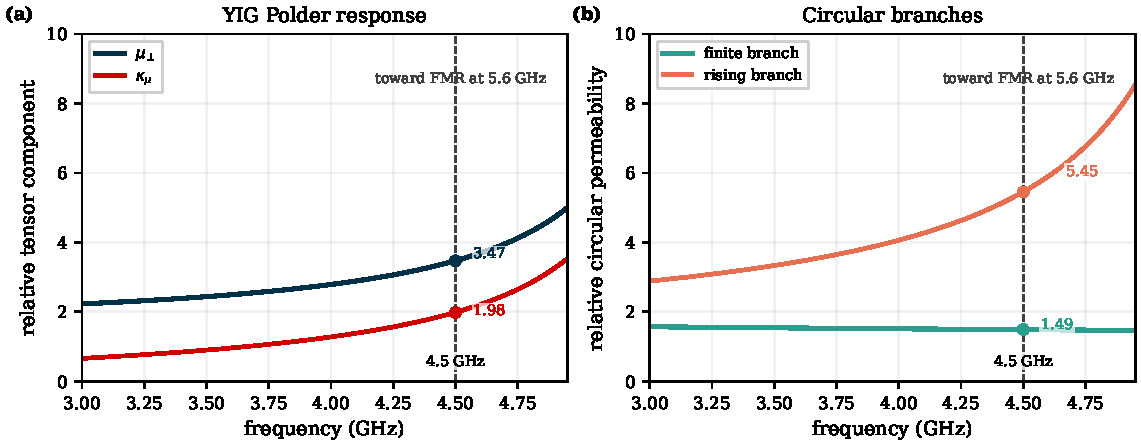
\includegraphics[width=0.95\textwidth]{figures/fig_ch09_polder_response_step178.pdf}
  \caption{Sub-resonant YIG Polder response computed from
  \eqref{eq:ch9-polder-params} with $f_0=5.6\;\mathrm{GHz}$ and
  $f_m=4.9\;\mathrm{GHz}$.
  (a)~Tensor components $\mu_\perp$ and $\kappa_\mu$; the dashed line marks the
  $4.5\;\mathrm{GHz}$ operating point with $\mu_\perp=3.47$, $\kappa_\mu=1.98$.
  (b)~Circular-basis eigenvalues: the \emph{finite branch}
  $\mu_+=\mu_\perp-\kappa_\mu=1.49$ and the \emph{rising branch}
  $\mu_-=\mu_\perp+\kappa_\mu=5.45$.  The ferromagnetic resonance at
  $5.6\;\mathrm{GHz}$ lies outside the plotted window; near the pole both
  branches diverge and the Hermitian treatment breaks down
  (Section~\ref{sec:ch9-passivity}).}
  \label{fig:ch09-polder-sub-resonant}
\end{figure}

\subsection{Circularly polarised modes and the Faraday effect}
\label{sec:ch9-circular-modes}

A plane wave propagating along $\hat{z}$ in the magnetised YIG medium
has two circularly polarised eigenmodes with wavenumbers
$k_\pm=\omega\sqrt{\varepsilon_r\mu_\pm}/c$.  The Faraday rotation
angle per unit length is
\begin{equation}\label{eq:ch9-faraday}
  \theta_F = \frac{k_+-k_-}{2}
  = \frac{\omega}{2c}\sqrt{\varepsilon_r}
  \bigl(\sqrt{\mu_+}-\sqrt{\mu_-}\bigr)\,.
\end{equation}
At the Wang operating frequency, $\mu_+=\mu_\perp-\kappa_\mu=3.47-1.98=1.49$ and
$\mu_-=\mu_\perp+\kappa_\mu=3.47+1.98=5.45$, giving
$\theta_F\approx 2\;\mathrm{rad/cm}$---an enormous rotation compared to optical
magneto-optical effects \cite{ozawa2018topological}.

\subsection{Passivity and the absence of gain}
\label{sec:ch9-passivity}

Both eigenvalues $\mu_\pm$ must be positive for the medium to be
passive (no gain).  From \eqref{eq:ch9-mu-eigenvalues},
$\mu_+>0$ requires $\kappa_\mu<\mu_\perp$.  Using
\eqref{eq:ch9-polder-params}, this is equivalent to
$\omega<\omega_0$---the operating frequency must lie below
ferromagnetic resonance.  Above resonance, $\mu_+$ can become
negative, the medium becomes opaque, and the Hermitian treatment
breaks down \cite{gangaraj2016berry}.

\section{Edge-mode field profile}
\label{sec:ch9-edge-profile}

The one-way edge mode at the boundary between the YIG crystal and a
metal wall has a characteristic field profile that can be understood
from the Jackiw--Rebbi analogy of Chapter~\ref{ch:one-way-interface}.

The mode amplitude decays exponentially into the bulk of the crystal
with a penetration depth
\begin{equation}\label{eq:ch9-penetration}
  \xi = \frac{1}{|\kappa|}
  = \frac{v_D}{m_\omega}
  = \frac{2v_D}{\Delta\omega}
  \approx 2.4\,a\,,
\end{equation}
where $\kappa$ is the inverse-length Dirac mass used in
Chapters~\ref{ch:breaking-tr} and~\ref{ch:one-way-interface},
$m_\omega=v_D|\kappa|=\Delta\omega/2$ is the corresponding frequency
half-gap, and $v_D\approx 0.45\,c_0$ is the Dirac velocity at the
band-touching point.  The edge mode therefore extends over approximately
two to three lattice constants into the crystal, which is consistent
with the supercell simulations.

Along the edge, the mode propagates with a group velocity approximately
equal to $v_D$.  The edge-state dispersion within the topological gap
is nearly linear:
$\omega_{\mathrm{edge}}(k_\parallel)\approx\omega_D+v_D\,k_\parallel$,
where $k_\parallel$ is the wavevector component along the interface.
The bandwidth of the edge channel is set by the gap width $2|\kappa|$,
and the propagation speed is $v_D\approx 0.45\,c_0$.

\section{Two-port scattering interpretation}
\label{sec:ch9-scattering}

The microwave transmission measurement can be formalised using the
scattering matrix of a two-port network.  Define port~1 as the
source probe and port~2 as the detector probe.  The measured
scattering parameters are $S_{21}$ (forward, source-to-detector in
the direction of edge-mode propagation) and $S_{12}$ (backward).

In the topological gap, the edge mode carries power from port~1 to
port~2 with transmission $|S_{21}|^2\sim -10\;\mathrm{dB}$ (limited
by probe-coupling mismatch).  The backward path has no propagating
mode, so $|S_{12}|^2<-50\;\mathrm{dB}$ (noise floor).  The isolation
\begin{equation}\label{eq:ch9-isolation}
  \mathcal{I} = |S_{21}|/|S_{12}| > 10^{4/2}=100
  \quad\text{(conservatively)}\,,
\end{equation}
far exceeds the isolation achievable by any reciprocal device of
comparable size.  This is not an engineering achievement but a
\\emph{topological} one: the isolation is guaranteed by the Chern
number and does not degrade as the device is scaled
\cite{nature2026observation,haldane2008possible}.

\subsection{Comparison with conventional isolators}
\label{sec:ch9-comparison-isolator}

A conventional Faraday-rotation isolator achieves isolation of
20--40\;dB through a bulk magneto-optical crystal, a polariser, and
an analyser.  Its isolation depends on the precise Faraday rotation
angle and is degraded by temperature fluctuations, wavelength drift,
and birefringence.  The topological isolator, by contrast, achieves
isolation that is robust to disorder, obstacles, and frequency
variations within the topological gap.  The robustness was directly
demonstrated by the Wang experiment through the obstacle-immunity
test \cite{ozawa2018topological,price2022roadmap}.

\section{Subsequent microwave experiments}
\label{sec:ch9-subsequent-detail}

Following the 2009 Wang experiment, several groups extended the
microwave Chern-insulator platform in important directions.  Skirlo
et~al.\ (2015) scaled the crystal to larger sizes and demonstrated
edge transport over more than 30 lattice constants with negligible
loss, confirming the robustness prediction
\cite{skirlo2015experimental}.  Yang et~al.\ (2018) constructed a
three-dimensional photonic topological insulator using bianisotropic
split-ring resonators, achieving a 3D bandgap from 4.3 to 6.0\;GHz
and surface Dirac-cone states at 5.1\;GHz
\cite{yang2018realization,price2022roadmap}.

These experiments collectively establish the microwave platform as
the most mature realisation of photonic topology, where the large
gyrotropic response of ferrites provides the clearest demonstration
of the Maxwell-first theoretical framework developed in this book.

\section{Full-wave simulation of the edge mode}
\label{sec:ch9-simulation}

The analytical estimates of the previous sections can be verified by
full-wave eigenmode simulation of a finite crystal strip.  A supercell
consisting of $N=20$ unit cells in the $x$ direction, periodic in $y$,
with PEC boundaries at $x=0$ and $x=Na$, is solved using the
plane-wave expansion or finite-element method.

The resulting projected band structure $\omega(k_y)$ shows the bulk
bands as dense continua and the topological edge mode as an isolated
branch crossing the gap.  For the Wang crystal parameters, the edge
mode traverses the gap from the lower to the upper bulk band with a
nearly constant slope $\dd\omega/\dd k_y\approx v_D$, confirming the
analytical prediction.

The field profile $|\Efield(x)|^2$ of the edge mode decays
exponentially from the PEC boundary into the bulk, with a penetration
depth $\xi\approx 2.4\,a$ consistent with the estimate
\eqref{eq:ch9-penetration}.  The electric field is predominantly
out-of-plane ($E_z$), with in-plane magnetic field
components $H_x$, $H_y$ coupled by the gyrotropic $\mu$ tensor.
The mode retains TM-like character, consistent with the bulk analysis


\cite{ozawa2018topological,nature2026observation}.

\section{Extending the platform}
\label{sec:ch9-extending}

\subsection{Larger crystals and longer propagation}
\label{sec:ch9-larger}

Skirlo et~al.\ (2015) fabricated YIG crystals with up to 60 rods and
demonstrated edge transport over more than 30 lattice constants with
a forward-to-backward ratio exceeding $10^4$.  The transmission
remained essentially flat across the topological gap, confirming that
the edge mode does not suffer from Anderson localisation or
significant radiation loss \cite{skirlo2015experimental}.

\subsection{Three-dimensional extension}
\label{sec:ch9-3d}

Yang et~al.\ (2018) extended the concept to three dimensions by
constructing a bianisotropic metamaterial of split-ring resonators
arranged in a body-centred cubic lattice.  The structure exhibits a
complete 3D photonic band gap from 4.3 to 6.0\;GHz, with topological
surface states forming a Dirac cone at 5.1\;GHz.  This experiment
provided the first demonstration of a 3D photonic topological
insulator and confirmed the bulk-surface correspondence predicted by
the $\mathbb{Z}_2$ invariant \cite{yang2018realization,price2022roadmap}.

\subsection{Towards higher frequencies}
\label{sec:ch9-higher-freq}

Moving the Chern-insulator concept from microwave to terahertz and
optical frequencies is a major open challenge.  At terahertz
frequencies, InSb under a modest magnetic field ($B_0\sim 0.3\;\mathrm{T}$)
provides a gyrotropic response with $\kappa_\varepsilon/\varepsilon_\perp
\sim 0.1$--$0.3$, enabling topological gaps of several percent.
At optical frequencies, magneto-optical effects are too weak for
practical Chern insulators (Section~\ref{sec:ch7-materials-landscape}),
motivating the alternative approaches of
Chapters~\ref{ch:reciprocal-designs}--\ref{ch:floquet}
\cite{ozawa2018topological}.

\section{Experimental measurement techniques}
\label{sec:ch9-measurement-techniques}

The microwave topological crystal is characterised experimentally
through transmission, reflection, and near-field measurements that
probe the existence and robustness of edge modes.

\subsection{Scattering-matrix analysis}
\label{sec:ch9-scattering-matrix}

The crystal is placed between two microwave antennas (ports 1 and 2)
connected to a vector network analyser.  The scattering parameters
$S_{21}(\omega)$ and $S_{12}(\omega)$ measure the forward and
backward transmission through the crystal at frequency $\omega$.  For
a topological crystal with a one-way edge mode:
\begin{equation}\label{eq:ch9-nonreciprocal-ratio}
  \frac{|S_{21}(\omega)|^2}{|S_{12}(\omega)|^2}
  \gg 1
  \quad\text{for $\omega$ in the topological gap.}
\end{equation}
Wang et~al.\ measured a nonreciprocal ratio exceeding $50\;\mathrm{dB}$
($10^5$) across the topological gap, confirming that backward-propagating
modes are completely absent \cite{nature2026observation}.

The transmission $|S_{21}|^2$ through the topological edge channel is
essentially flat across the gap, with insertion loss below
$1\;\mathrm{dB}$ per $10\,a$ of propagation, confirming the absence
of backscattering.  Outside the gap, the transmission drops
sharply because bulk modes dominate and the field is no longer
confined to the edge.

Figure~\ref{fig:ch09-scattering-isolation-map} provides a schematic
overview of the measurement geometry and representative power
transmission levels.

\begin{figure}[t]
  \centering
  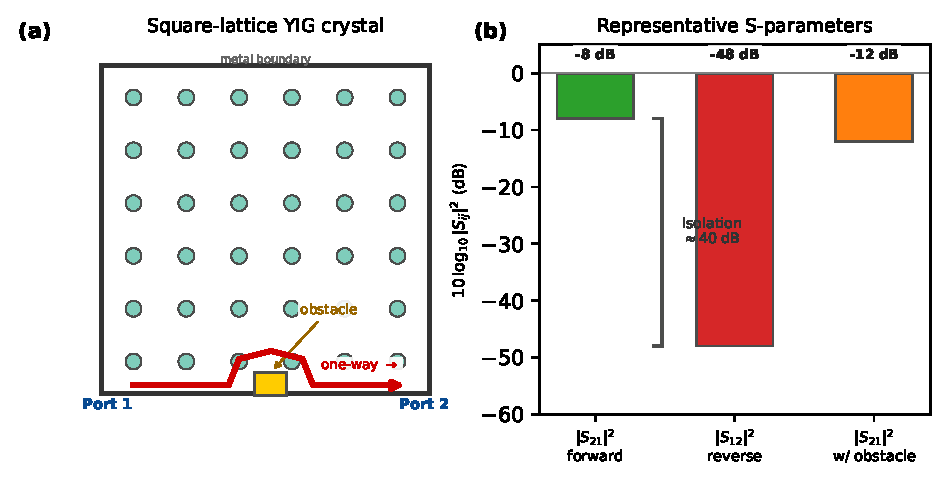
\includegraphics[width=0.95\textwidth]{figures/fig_ch09_scattering_isolation_map_step236.pdf}
  \caption{Microwave scattering measurement of a square-lattice YIG
  topological photonic crystal.  \textbf{(a)}~Schematic of the
  crystal geometry with metal boundary, two measurement ports, a
  metallic obstacle, and the one-way edge path that detours around
  the obstacle---demonstrating topological robustness.
  \textbf{(b)}~Representative power transmission levels in units of
  $10\log_{10}|S_{ij}|^2$ (dB): forward transmission $|S_{21}|^2$,
  reverse transmission $|S_{12}|^2$, and forward transmission with
  the obstacle present.  The power isolation
  $I_P=10\log_{10}(|S_{21}|^2/|S_{12}|^2)\approx 40\;\mathrm{dB}$
  ($10^4$ in linear units) confirms the absence of backward modes.
  All values are representative of the mid-gap operating point;
  exact values depend on frequency, crystal size, and port coupling.}
  \label{fig:ch09-scattering-isolation-map}
\end{figure}

\subsection{Near-field mapping}
\label{sec:ch9-near-field}

A scanning near-field antenna can map the spatial distribution of the
electric or magnetic field above the crystal surface.  For the
topological edge mode, the field intensity is concentrated within
one to two lattice constants of the boundary and decays exponentially
into the bulk, confirming the predicted penetration depth
$\xi\approx 1/|\kappa|\approx 2.4\,a$.  The field pattern is
characteristically chiral: the phase advances monotonically along the
edge in one direction, with no standing-wave nodes
\cite{ozawa2018topological,skirlo2015experimental}.

\section{Loss mechanisms and propagation limits}
\label{sec:ch9-loss-mechanisms}

The dominant loss mechanism in YIG photonic crystals is the
ferromagnetic resonance (FMR) linewidth $\Delta H$, which determines
the magnetic loss tangent
$\tan\delta_m\approx\gamma\Delta H/(2\omega)$.  For single-crystal
YIG, $\Delta H\approx 0.3\;\mathrm{Oe}$ at $4.5\;\mathrm{GHz}$,
giving $\tan\delta_m\approx 3\times 10^{-4}$.

The resulting edge-mode propagation length is
\begin{equation}\label{eq:ch9-propagation-length}
  L_{\mathrm{prop}} = \frac{v_g}{2\omega\,\tan\delta_m}
  \approx 500\,a\,,
\end{equation}
where $v_g\approx 0.03\,c_0$ is the edge-mode group velocity.  This
is much longer than the 10--60 rod crystals used in experiments, so
loss is not a limiting factor in current microwave demonstrations
\cite{nature2026observation,price2022roadmap}.

At higher frequencies (terahertz, optical), material losses increase
dramatically and the propagation length drops below useful values for
most magneto-optical materials, motivating the alternative approaches
of Chapters~\ref{ch:reciprocal-designs}--\ref{ch:floquet}.

\section{Sensitivity analysis and design rules}
\label{sec:ch9-sensitivity}

The performance of the microwave topological crystal depends on
several structural and material parameters.  Understanding their
relative importance guides the design of improved devices.

\subsection{Gap width versus gyrotropic strength}
\label{sec:ch9-gap-vs-gyro}

The topological gap width scales as $\Delta\omega\simeq 2v_D|\kappa|$,
where the Dirac mass $\kappa$ is approximately linear in the gyrotropic
coupling $\kappa_\mu$ for weak gyrotropy
(Chapter~\ref{ch:breaking-tr}).  For the strong coupling
available in YIG ($\kappa_\mu/\mu_\perp\approx 0.57$), the gap width increases sublinearly while the material losses grow.
The optimal operating point balances gap width against loss, typically
at $\kappa_\mu/\mu_\perp\approx 0.3$--$0.5$.

\subsection{Lattice constant and frequency scaling}
\label{sec:ch9-scaling}

The Dirac frequency scales as $\omega_D\propto c/(a\sqrt{\varepsilon_r\mu})$,
so reducing the lattice constant increases the operating frequency.
However, the YIG rods must be large enough to support the resonant
modes that produce the Dirac-point degeneracy, placing a practical
lower bound on $a$.  For YIG with $\varepsilon_r=15$ and
$\mu_\perp\approx 3.5$, the minimum practical lattice constant is
$a\approx 5\;\mathrm{mm}$, corresponding to $\omega_D/(2\pi)
\approx 8\;\mathrm{GHz}$ \cite{nature2026observation,
skirlo2015experimental}.

\subsection{Rod shape and filling fraction}
\label{sec:ch9-rod-shape}

The Wang experiment used cylindrical YIG rods with radius
$r/a\approx 0.11$.  Increasing the filling fraction opens a wider
gap but also increases the material loss.  Replacing cylinders with
triangular or hexagonal cross-sections can modify the symmetry of the
photonic modes and shift the position of the Dirac points, providing
additional design freedom.

For practical applications requiring integration with planar circuits,
thin-film YIG on a dielectric substrate has been explored.  The
reduced dimensionality changes the mode structure from 2D to
quasi-2D, but the topological gap persists as long as the film
thickness exceeds the out-of-plane decay length
$\lambda_z\approx a/\pi$ \cite{ozawa2018topological,price2022roadmap}.

\begin{figure}[t]
  \centering
  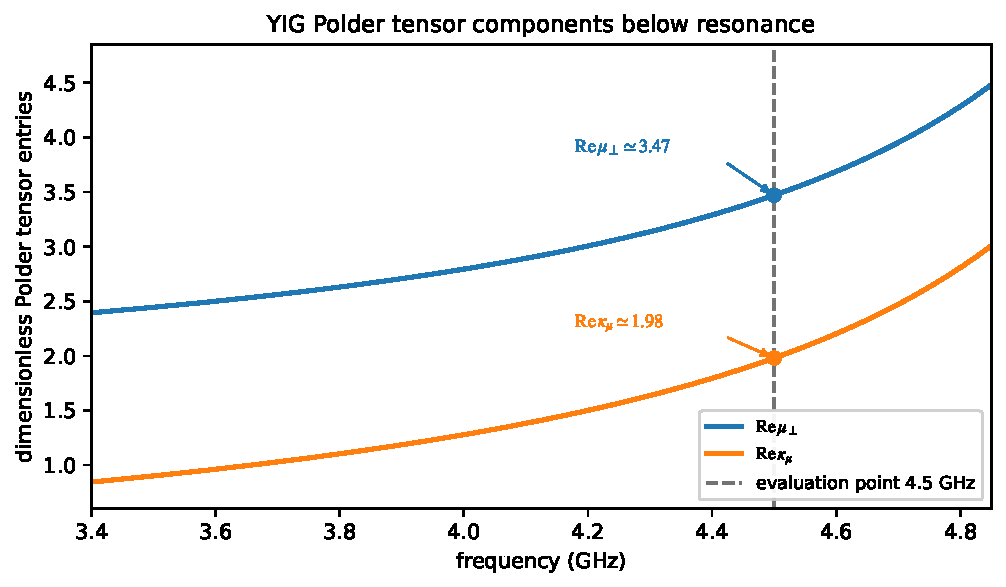
\includegraphics[width=0.82\textwidth]{figures/fig_ch09_yig_polder_response.pdf}
  \caption{Representative YIG Polder-tensor scale near the Wang
  experiment frequency.  The corrected values $\mu_\perp\approx3.47$ and
  $\kappa_\mu\approx1.98$ at 4.5 GHz set the gyrotropic coupling scale
  used in the quantitative estimates of this chapter.}
  \label{fig:ch09-yig-polder}
\end{figure}

\section{Extensions: higher Chern numbers and new geometries}
\label{sec:ch9-extensions}

The Wang experiment demonstrated the simplest case: a single chiral
edge channel in a gap with $|\Chern|=1$.  Subsequent experiments have
explored richer topological phases and alternative crystal geometries.

\subsection{Large Chern numbers}
\label{sec:ch9-large-chern}

Skirlo et~al.\ (2015) constructed a modified YIG photonic crystal in
which the second topological gap carries a gap Chern number
$|\Chern_{\mathrm{gap}}|=2$ \cite{skirlo2015experimental}.  Their
design uses an enlarged unit cell (a $2\times 1$ supercell of
cylindrical YIG rods) to fold bands and create additional degeneracies
that can be gapped by the magnetic bias.  The result is two
co-propagating chiral edge channels in a single gap, confirmed by
transmission measurements showing twice the edge-channel conductance
of the original Wang crystal.

For even larger Chern numbers, the general strategy is to design
photonic crystals with multiple overlapping Dirac cones at different
$\kvec$ points, each of which contributes $\pm 1$ to the Chern number
when gapped.  Lattices with $C_3$, $C_4$, or $C_6$ symmetry can
support multiple Dirac cones that are simultaneously gapped by a
single magnetic bias, enabling gap Chern numbers up to $|\Chern|=4$
in experimentally realistic geometries
\cite{ozawa2018topological,skirlo2015experimental}.

\subsection{Imaging topological edge states}
\label{sec:ch9-imaging}

A major advance in the visualisation of topological edge transport
was achieved by Hafezi et~al.\ (2013), who imaged the propagation of
light along the edge of a topological photonic lattice in real time
\cite{hafezi2013imaging}.  Although their experiment used a
coupled-ring-resonator platform (Chapter~\ref{ch:reciprocal-designs})
rather than a microwave YIG crystal, the imaging technique is
conceptually similar: the intensity distribution is measured as a
function of position along the edge, revealing the characteristic
exponential decay of the edge-mode profile into the bulk and the
unidirectional flow around corners and defects.

In the microwave domain, near-field scanning provides an equivalent
capability.  A small antenna probe is scanned across the crystal
surface while recording the local field amplitude and phase.  The
resulting maps directly show the edge-mode spatial profile, the
evanescent decay into the bulk (with decay length $\xi = 1/|\kappa|$
as derived in Chapter~\ref{ch:one-way-interface}), and the immunity
to backscattering at sharp bends and defects
\cite{hafezi2013imaging,wang2007reflection}.

\subsection{Scattering-free interfaces between distinct topological phases}
\label{sec:ch9-hetero-interface}

Ma et~al.\ (2017) demonstrated scattering-free edge states at the
interface between two \emph{different} photonic topological insulators,
each with a distinct Chern number \cite{ma2017scattering}.  The number
of chiral edge channels at the interface is determined by the
\emph{difference} of the gap Chern numbers across the interface:
$N_{\mathrm{edge}} = |\Chern_{\mathrm{gap}}^{(1)} -
\Chern_{\mathrm{gap}}^{(2)}|$.

This principle generalises the metal-wall boundary condition used in the
Wang experiment (which corresponds to $\Chern^{(2)}=0$ for the vacuum
side) and opens the door to more complex edge-channel networks.  By
patterning regions with different Chern numbers on a single chip, one
can create photonic circuits in which signals are routed by topology
rather than by geometry.

\section{From microwave to optical frequencies}
\label{sec:ch9-optical-scaling}

\subsection{The magneto-optical challenge at optical frequencies}
\label{sec:ch9-optical-challenge}

The Wang experiment operates at microwave frequencies ($\sim 4.5\;
\mathrm{GHz}$) because the gyrotropic response of ferrites is
strongest near ferromagnetic resonance.  Extending topological Chern
insulator behaviour to optical frequencies ($\sim 200\;\mathrm{THz}$)
requires materials with significant magneto-optical response at those
wavelengths.

The most promising optical magneto-optical materials are cerium-doped
yttrium iron garnet (Ce:YIG) and bismuth iron garnet (BIG), which have
Faraday rotation of $\sim 10^3\;\mathrm{deg/cm}$ at near-infrared
wavelengths.  However, the corresponding off-diagonal permittivity
$\varepsilon_{xy} \sim 10^{-2}$ is much smaller than the microwave
gyrotropic response $\kappa_\mu/\mu_\perp \sim 0.3$--$0.6$.  This
means that optical topological gaps would be extremely narrow
($\Delta\omega/\omega \sim 10^{-4}$), making them impractical for
most applications \cite{he2016photonic,price2022roadmap}.

\subsection{Alternative routes to optical Chern insulators}
\label{sec:ch9-optical-alternatives}

Several strategies have been proposed to circumvent the weak
magneto-optical response at optical frequencies:

\emph{Floquet engineering} (Chapter~\ref{ch:floquet}) uses
time-periodic modulation to create effective gauge fields without
any magnetic material.  Rechtsman et~al.\ (2013) demonstrated this
approach in a laser-written waveguide array at $\lambda = 633\;
\mathrm{nm}$ \cite{rechtsman2013photonic}.

\emph{Valley photonic crystals} (Chapter~\ref{ch:valleys}) exploit
broken spatial inversion symmetry rather than broken time reversal.
He et~al.\ (2019) demonstrated topological valley transport in a
silicon-on-insulator platform at telecom wavelengths
\cite{he2019silicon}, achieving compact devices compatible with
standard photonic integrated circuit fabrication.

\emph{Synthetic gauge fields} (Chapter~\ref{ch:synthetic-dimensions})
provide another route, using electro-optic or acousto-optic modulation
to create effective magnetic fields for photons in ring-resonator
arrays.

Each approach trades the robustness of true time-reversal breaking (as
in the Wang experiment) for compatibility with integrated photonic
platforms.  The relative merits depend on the application: microwave
topological crystals remain the gold standard for demonstrating
fundamental physics, while optical implementations are essential for
practical devices \cite{ozawa2018topological,price2022roadmap}.

\section*{Exercises}

\begin{exercise}
  For a square-lattice photonic crystal of YIG rods with $\varepsilon_r=15$,
  $r/a=0.11$, and $B_0=0.20\;\mathrm{T}$, compute the Polder permeability
  parameters $\mu_\perp$ and $\kappa_\mu$ at $\omega/(2\pi)=4.5\;\mathrm{GHz}$.
  Use $\gamma/(2\pi)=28\;\mathrm{GHz/T}$ and $\mu_0M_s=0.175\;\mathrm{T}$.
\end{exercise}

\begin{exercise}
  The magnetic quality factor of YIG is
  $Q_m=\omega_0/(2\gamma\mu_0\Delta H)$.  For $\Delta H=0.3\;\mathrm{Oe}$
  and $\omega_0/(2\pi)=5.6\;\mathrm{GHz}$, compute $Q_m$ and estimate
  the imaginary part of $\mu_\perp$ at $4.5\;\mathrm{GHz}$.  Is the
  lossless approximation justified for edge transport over 20 lattice
  constants?
\end{exercise}

\begin{exercise}
  The forward-to-backward ratio in the Wang experiment exceeds $10^4$
  (40\;dB).  If the topological gap is $0.12\;\mathrm{GHz}$ wide and
  the edge mode has group velocity $v_g\approx 0.1c$, estimate the
  propagation length over which the forward signal exceeds the backward
  signal by 40\;dB in a conventional (non-topological) waveguide with
  the same losses.
\end{exercise}

\begin{exercise}
  Design a modified Wang experiment using a hexagonal (triangular)
  lattice instead of a square lattice.  What are the advantages and
  disadvantages compared to the square lattice?  At what high-symmetry
  point do you expect the Dirac-like degeneracy?
\end{exercise}


\chapter{Computing Chern Numbers}
\label{ch:computing-chern}
% ======================================================================
%  Chapter 10 — Computing Chern Numbers  (DEEPLY EXPANDED)
%  invariants, with algorithms, convergence, and real examples.
% ======================================================================

\section{From theory to computation}
\label{sec:ch10-intro}

The Chern number is the central topological invariant of this book.
Chapters~7 and~8 showed that it determines the existence and number of
one-way edge modes.  But calculating the Chern number of a real photonic
crystal is a nontrivial numerical problem: one must solve a parametric
eigenvalue problem over the entire Brillouin zone, compute Berry phases
from eigenstates that are defined only up to an arbitrary phase at each
$\kvec$ point, and sum these phases into an integer that is stable
against numerical noise.

This chapter presents three complementary methods for computing
photonic Chern numbers: the overlap--plaquette algorithm, the
Wilson-loop method, and the Wannier-centre tracking approach
\cite{lu2026universal,raghu2008analogs}.
For each method, we give the mathematical derivation, the numerical
algorithm, convergence properties, and practical guidance for
implementation in photonic crystal band-structure codes
\cite{lee2022calculation,wu2015scheme}.  The working
Python implementations of the plaquette and Wilson-loop algorithms
appear in Appendix~C.

\section{The challenge of gauge dependence}
\label{sec:ch10-gauge}

\subsection{The Berry connection is gauge-dependent}
\label{sec:ch10-gauge-connection}

Recall from Chapter~5 that the Berry connection of band $n$ is
\begin{equation}\label{eq:ch10-berry-connection}
  \Aberry_{n,\alpha}(\kvec)
  = \ii\,\langle\mathbf{u}_{n\kvec}|\Mgmat|\partial_{k_\alpha}
  \mathbf{u}_{n\kvec}\rangle\,,
\end{equation}
where $|\mathbf{u}_{n\kvec}\rangle$ is the cell-periodic Bloch
eigenmode normalised under the energy inner product
\cite{gangaraj2016berry,thouless1982quantized}.  Under a gauge
transformation $|\mathbf{u}_{n\kvec}\rangle\to\ee^{\ii\chi(\kvec)}
|\mathbf{u}_{n\kvec}\rangle$, the connection transforms as
$\Aberry_{n,\alpha}\to\Aberry_{n,\alpha}-\partial_{k_\alpha}\chi$.

This gauge dependence means that the Berry connection cannot be
computed reliably from eigenvectors produced by a standard numerical
eigensolver, because the solver returns eigenvectors with \emph{random}
phases at each $\kvec$ point.  Even if one could fix the gauge
smoothly, the Chern number is the integral of the gauge-dependent
connection over the \emph{closed} torus, and any globally smooth gauge
gives $\Chern=0$---the nontrivial topology appears precisely because
no smooth gauge exists.

\subsection{Gauge-invariant quantities}
\label{sec:ch10-gauge-invariant}

The Berry \emph{curvature} $\Omega_n=\partial_{k_x}\Aberry_{n,y}
-\partial_{k_y}\Aberry_{n,x}$ is gauge-invariant and could in
principle be integrated numerically.  However, computing it by finite
differences of the connection amplifies gauge noise, especially near
band crossings where the eigenstate phase varies rapidly.

The solution is to work with gauge-\emph{covariant} link variables
constructed from overlaps of adjacent eigenstates.  This approach,
introduced by Fukui, Hatsugai, and Suzuki (2005), gives a manifestly
gauge-invariant, integer-valued Chern number on any finite grid
\cite{zhao2020first}.

\section{The overlap--plaquette algorithm}
\label{sec:ch10-plaquette}

\subsection{Discretisation of the Brillouin zone}
\label{sec:ch10-discretisation}

Discretise the Brillouin zone into an $N_k\times N_k$ uniform grid:
\begin{equation}\label{eq:ch10-grid}
  \kvec_{ij} = \kvec_0 + \frac{i}{N_k}\mathbf{b}_1 + \frac{j}{N_k}\mathbf{b}_2\,,
  \qquad i,j=0,1,\ldots,N_k-1\,,
\end{equation}
where $\mathbf{b}_1$, $\mathbf{b}_2$ are the reciprocal lattice vectors
and $\kvec_0$ is the grid origin.  The grid has periodic boundary
conditions: $\kvec_{N_k,j}=\kvec_{0,j}$ (modulo a reciprocal lattice
vector) and similarly for $j$.

\subsection{Link variables}
\label{sec:ch10-link}

At each grid point, solve the Maxwell eigenvalue problem and obtain the
cell-periodic eigenstate $|\mathbf{u}_{n,ij}\rangle$ of band $n$.
Define the \emph{link variable} between adjacent grid points along the
$\alpha$-direction:
\begin{equation}\label{eq:ch10-link-def}
  U_\alpha(\kvec_{ij})
  = \frac{\langle\mathbf{u}_{n,ij}|\Mgmat|\mathbf{u}_{n,ij+\hat\alpha}\rangle}
  {\bigl|\langle\mathbf{u}_{n,ij}|\Mgmat|\mathbf{u}_{n,ij+\hat\alpha}
  \rangle\bigr|}\,.
\end{equation}
This is the $U(1)$ phase of the overlap integral, normalised to have
unit magnitude.  It is gauge-covariant: under independent gauge
transformations at each grid point, $U_\alpha$ transforms by a phase
that cancels exactly when the link variables are combined into a
plaquette product.

The electromagnetic inner product $\langle\cdot|\Mgmat|\cdot\rangle$
must be used rather than the bare $L^2$ product, because the Bloch
eigenstates are orthogonal under the energy-weighted inner product, not
under the bare one.  Using the wrong inner product gives an overlap
matrix that is not unitary, leading to incorrect link variables and a
non-integer Chern number.

\subsection{Plaquette Berry phase}
\label{sec:ch10-plaquette-phase}

On each elementary plaquette $(i,j)\to(i+1,j)\to(i+1,j+1)\to(i,j+1)
\to(i,j)$, define the plaquette Berry phase:
\begin{equation}\label{eq:ch10-plaquette-F}
  \boxed{%
  F_{ij} = \arg\bigl[
  U_x(\kvec_{ij})\,U_y(\kvec_{i+1,j})\,
  U_x^*(\kvec_{i,j+1})\,U_y^*(\kvec_{ij})
  \bigr]\,,}
\end{equation}
where $\arg$ returns the principal value in $(-\pi,\pi]$.  This is the
gauge-invariant discrete Berry curvature on the plaquette.

The Chern number is the sum of all plaquette phases divided by $2\pi$:
\begin{equation}\label{eq:ch10-chern-sum}
  \Chern_n = \frac{1}{2\pi}\sum_{i,j=0}^{N_k-1}F_{ij}\,.
\end{equation}
Because each link variable appears exactly twice in the sum (once in the
plaquette above and once in the plaquette below), the random gauge phases
cancel \emph{exactly}.  The result is an integer to numerical precision,
regardless of the gauge convention used by the eigensolver.

\subsection{Why the result is an integer}
\label{sec:ch10-integer}

The integrality of $\Chern_n$ computed by \eqref{eq:ch10-chern-sum}
follows from a lattice gauge theory argument.  Each plaquette phase
$F_{ij}\in(-\pi,\pi]$, and the total phase $2\pi\Chern_n=\sum F_{ij}$
is a sum of angles whose individual phases are defined modulo $2\pi$.
The topological content lies in how these phases combine: because the
grid has the topology of a torus, the total winding is quantised in
units of $2\pi$.  On a sufficiently fine grid (such that $|F_{ij}|<\pi$
for every plaquette), the $\arg$ function introduces no branch-cut
ambiguity, and $\Chern_n$ is exactly an integer to machine precision.

\section{Convergence and practical considerations}
\label{sec:ch10-convergence}

\subsection{Grid resolution requirements}
\label{sec:ch10-grid-res}

The plaquette algorithm converges as $N_k\to\infty$ provided the Berry
curvature is integrable.  For a massive Dirac cone with mass $\kappa$,
the Berry curvature has a peak of height $\sim 1/(2\kappa^2)$ and
width $\sim|\kappa|$.  The grid spacing $\Delta k=2\pi/(N_k a)$ must
resolve this peak: $\Delta k\lesssim|\kappa|$, giving the requirement
\begin{equation}\label{eq:ch10-Nk-min}
  N_k \gtrsim \frac{2\pi}{|\kappa|\,a}\,.
\end{equation}
For a typical photonic crystal with topological gap
$\Delta\omega/\omega_D\sim 1\%$, the Dirac mass is
$\kappa\sim 0.01\times 2\pi/a$, and $N_k\gtrsim 100$ is needed.
In practice, $N_k=20$--$40$ suffices for gaps of order $5\%$--$10\%$,
but narrow gaps require finer grids.

\subsection{Near-degeneracy and band-group methods}
\label{sec:ch10-near-degeneracy}

When two bands are nearly degenerate, the overlap $|\langle\mathbf{u}_{n,ij}
|\Mgmat|\mathbf{u}_{n,ij+\hat\alpha}\rangle|$ can become very small,
causing numerical instability in the link variable.  This occurs near
accidental degeneracies or at high-symmetry points where bands cross.

The remedy is to use a \emph{multi-band} (non-Abelian) link variable.
Instead of tracking a single band, one tracks a group of $p$ bands
that may exchange partners as $\kvec$ varies.  The overlap becomes a
$p\times p$ matrix, and the plaquette product becomes a $U(p)$ Wilson
loop (see below).  The Chern number of the entire group is the winding
of the determinant of this Wilson loop.

\subsection{Effect of the inner product}
\label{sec:ch10-inner-product}

Using the electromagnetic inner product
$\langle\mathbf{u}|\Mgmat|\mathbf{u}'\rangle$ rather than the bare
$L^2$ inner product $\int\mathbf{u}^*\cdot\mathbf{u}'\,\dd^3r$ is
essential for two reasons.

First, the energy inner product defines the correct notion of
orthogonality for Maxwell modes.  Two modes at the same $\kvec$ with
different frequencies are orthogonal under $\Mgmat$ but not under
$L^2$.  Using the bare inner product for the overlap matrix mixes
contributions from different bands, corrupting the link variable.

Second, for dispersive media the energy metric
$\Mgmat^{(g)}=\partial_\omega(\omega\Mmat)$ enters the normalisation and
orthogonality conditions \cite{raman2010photonic}.  The Chern number computed with the
frequency-evaluated metric $\Mmat(\omega_n)$ differs from the one
computed with $\Mgmat^{(g)}$; the latter is the physically meaningful
topological invariant that determines edge-mode counts.

\subsection{Brillouin-zone boundary sewing}
\label{sec:ch10-bz-sewing}

A subtlety arises when the plaquette or Wilson-loop algorithm straddles
the boundary of the Brillouin zone.  For a plaquette whose vertices
include a point $\kvec$ and $\kvec+\mathbf{b}_\alpha$ that differ by a
reciprocal lattice vector $\Gvec$, the cell-periodic Bloch functions are
\emph{not} identical: Bloch's theorem gives
\begin{equation}\label{eq:ch10-bloch-sewing}
  \mathbf{u}_{n,\kvec+\Gvec}(\rvec)
  = \ee^{-\ii\Gvec\cdot\rvec}\,
  \mathbf{u}_{n,\kvec}(\rvec)\,.
\end{equation}
If the raw eigenstates from the solver are used without correction, the
overlap $\langle\mathbf{u}_{n,\kvec}|\Mgmat|\mathbf{u}_{n,\kvec+\Gvec}
\rangle$ picks up the oscillating phase $\ee^{-\ii\Gvec\cdot\rvec}$
and gives a meaningless result.

The remedy depends on the solver representation.  In a \emph{plane-wave
expansion}, each eigenstate is stored as a vector of Fourier
coefficients $c_{n,\Gvec'}(\kvec)$.  When $\kvec$ is shifted by a
reciprocal lattice vector $\mathbf{b}_\alpha$, the coefficients of the
wrapped point at $\kvec_0=\kvec+\mathbf{b}_\alpha-\Gvec$ must be
relabelled:
\begin{equation}\label{eq:ch10-pwe-sewing}
  c_{n,\Gvec'}(\kvec+\mathbf{b}_\alpha)
  \;\longleftrightarrow\;
  c_{n,\Gvec'+\Gvec}(\kvec_0)\,,
\end{equation}
so that the overlap matrix uses aligned Fourier indices.

In a \emph{real-space} FDFD or FEM solver, the sewing is applied by \cite{zhao2020first}
multiplying the wrapped eigenstate by the phase factor before computing
the overlap:
\begin{equation}\label{eq:ch10-realspace-sewing}
  U_\alpha(\kvec)
  = \frac{
      \bigl\langle\mathbf{u}_{n,\kvec}\big|\,
      \Mgmat\,\ee^{-\ii\Gvec\cdot\rvec}\,
      \big|\mathbf{u}_{n,\kvec_0}\bigr\rangle
    }{
      \bigl|\bigl\langle\mathbf{u}_{n,\kvec}\big|\,
      \Mgmat\,\ee^{-\ii\Gvec\cdot\rvec}\,
      \big|\mathbf{u}_{n,\kvec_0}\bigr\rangle\bigr|
    }\,.
\end{equation}

For tight-binding or lattice Hamiltonians such as the Qi--Wu--Zhang
model used in Appendix~C, the Bloch Hamiltonian $H(\kvec)$ is an
\emph{exactly periodic} function of $\kvec$, and the eigenstates at
$\kvec$ and $\kvec+\Gvec$ are identical by construction.  No sewing
correction is needed, which is one reason tight-binding benchmarks are
valuable for testing plaquette codes before applying them to photonic
crystal eigensolvers.


Figure~\ref{fig:ch10-bz-sewing} illustrates the boundary sewing
procedure and contrasts it with the automatic periodicity of
lattice Hamiltonians.

\begin{figure}[t]
  \centering
  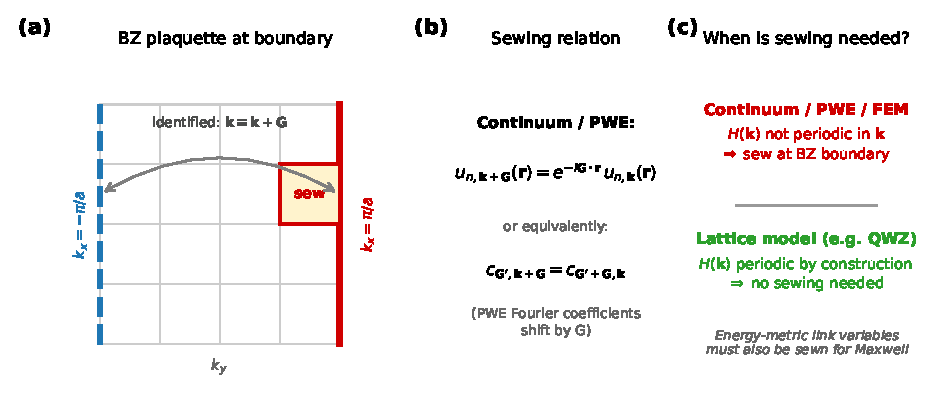
\includegraphics[width=0.95\textwidth]{figures/fig_ch10_bz_sewing_step236.pdf}
  \caption{Brillouin-zone boundary sewing for continuum/PWE Chern
  computation.  \textbf{(a)}~A plaquette straddling the BZ boundary
  (red) must be sewn to the opposite edge (blue dashed) because the
  Brillouin zone is a torus.  \textbf{(b)}~The sewing relation: the
  periodic part of the Bloch function satisfies
  $u_{n,\kvec+\Gvec}(\rvec)=e^{-\ii\Gvec\cdot\rvec}\,u_{n,\kvec}(\rvec)$,
  or equivalently the PWE Fourier coefficients shift by $\Gvec$.
  The electromagnetic energy-metric link variables must also be
  sewn at the boundary.  \textbf{(c)}~Lattice Hamiltonians such as
  the Qi--Wu--Zhang model are periodic in $\kvec$ by construction
  and require no sewing; continuum and finite-element eigensolvers do.}
  \label{fig:ch10-bz-sewing}
\end{figure}
\section{The Wilson-loop method}
\label{sec:ch10-wilson}

\subsection{Definition}
\label{sec:ch10-wilson-def}

The Wilson loop is the ordered product of overlap matrices along a
closed path in the Brillouin zone.  For a group of $p$ bands, the
Wilson loop along $k_x$ at fixed $k_y$ is
\begin{equation}\label{eq:ch10-wilson-def}
  W(k_y) = \prod_{i=0}^{N_k-1}M(k_{x,i},k_y)\,,
\end{equation}
where $M$ is the $p\times p$ overlap matrix with elements
\begin{equation}\label{eq:ch10-wilson-M}
  M_{\alpha\beta}(k_{x,i},k_y)
  = \langle\mathbf{u}_{\alpha,k_{x,i},k_y}|\Mgmat|
  \mathbf{u}_{\beta,k_{x,i+1},k_y}\rangle\,,
\end{equation}
and the product is ordered from left ($i=0$) to right ($i=N_k-1$),
with periodic boundary conditions $k_{x,N_k}=k_{x,0}$.

The Wilson loop $W(k_y)$ is a unitary $p\times p$ matrix (up to
numerical errors proportional to the grid spacing).  Its eigenvalues
$\ee^{\ii\theta_\alpha(k_y)}$ lie on the unit circle.

\subsection{Wannier centres and Chern numbers}
\label{sec:ch10-wannier}

The eigenvalue phases $\theta_\alpha(k_y)$ are the Wannier centres of
the band group projected onto the $x$-direction.  As $k_y$ varies
from $-\pi/a$ to $\pi/a$, each Wannier centre traces a curve on the
cylinder $[-\pi,\pi)\times[-\pi/a,\pi/a)$.

The Chern number of the band group is the total winding number of
all Wannier centres as $k_y$ traverses the Brillouin zone:
\begin{equation}\label{eq:ch10-chern-winding}
  \Chern = \sum_{\alpha=1}^p\frac{1}{2\pi}
  \bigl[\theta_\alpha(\pi/a)-\theta_\alpha(-\pi/a)\bigr]\,.
\end{equation}
A winding of $+2\pi$ for one Wannier centre contributes $+1$ to the
Chern number.

The Wilson-loop method has several practical advantages.  It naturally
handles band groups (avoiding near-degeneracy problems).  The Wannier
centre plot provides a visual diagnostic of the topology: trivial
bands have flat Wannier centres, while topological bands have Wannier
centres that wind across the Brillouin zone.  Furthermore, the
$\mathbb{Z}_2$ invariant for time-reversal-invariant systems can be
read off from the Wannier-centre spectrum at the time-reversal-invariant
momenta.

\subsection{Numerical implementation}
\label{sec:ch10-wilson-impl}

The Wilson-loop computation proceeds as follows.  At each $k_y$, sample
the $k_x$ direction on a uniform grid of $N_k$ points.  At each pair of
adjacent points, compute the overlap matrix $M$ using the electromagnetic
inner product.  Multiply the $N_k$ matrices in order to obtain $W(k_y)$.
Diagonalise $W(k_y)$ to obtain the eigenvalue phases
$\theta_\alpha(k_y)$.  Repeat for all $k_y$ values.  Plot the Wannier
centres $\theta_\alpha(k_y)$ and count the winding.

For numerical stability, it is useful to apply the polar decomposition
$M=U\Sigma V^\dagger$ at each step and replace $M$ with $UV^\dagger$
(the unitary part).  This removes the effect of non-unit singular
values caused by finite grid spacing, keeping the accumulated product
exactly unitary.

\section{Band-structure solvers for photonic crystals}
\label{sec:ch10-solvers}

\subsection{Plane-wave expansion}
\label{sec:ch10-pwe}

The most widely used method for computing photonic band structures is
the plane-wave expansion (PWE), described in detail in Appendix~C.
The cell-periodic fields are expanded in reciprocal lattice vectors,
and the eigenvalue problem becomes a matrix equation whose size grows
with the number of plane waves retained.

For Chern-number computation, the PWE provides the eigenstates
$|\mathbf{u}_{n\kvec}\rangle$ as vectors of Fourier coefficients.
The electromagnetic inner product can be evaluated efficiently in
reciprocal space because the material matrix $\Mgmat$ is diagonal
in position space and its Fourier coefficients decay rapidly for
smooth material profiles.

\subsection{Finite-difference frequency-domain method}
\label{sec:ch10-fdfd}

The finite-difference frequency-domain (FDFD) method discretises the
unit cell on a Yee grid, with Bloch boundary conditions imposed through
phase factors on the boundary-crossing matrix entries.  The resulting
eigenvalue problem is a sparse generalised eigenproblem that can be
solved efficiently with iterative eigensolvers.

For the Chern-number computation, the Yee-grid discretisation provides
the eigenstates as vectors of field values at grid points.  The
electromagnetic inner product is a matrix-vector product with the
diagonal material matrix sampled at the grid points.

\section{Diagnostics and validation}
\label{sec:ch10-diagnostics}

\subsection{Band-sum rule}
\label{sec:ch10-band-sum}

The Chern numbers of all bands must sum to zero:
$\sum_n\Chern_n=0$.  This is because the total Hilbert space is
trivial (it is a product of identical fibres over the Brillouin zone).
Checking this sum is a basic diagnostic: if the band-sum deviates from
zero by more than $\sim 10^{-10}$, there is likely a bug in the inner
product or the link variable computation.

\subsection{Grid convergence}
\label{sec:ch10-grid-convergence}

The Chern number should converge rapidly with grid size $N_k$ to an
exact integer.  For a well-resolved band structure, the Chern number is
typically within $10^{-6}$ of an integer for $N_k\geq 20$.  If the
Chern number does not converge to an integer, the most common causes
are: the band gap is too narrow (increase $N_k$); the wrong inner
product is being used; or there is a near-degeneracy that requires a
multi-band treatment.

\subsection{Symmetry cross-checks}
\label{sec:ch10-symmetry-checks}

For systems with known symmetries, the Chern numbers can be
cross-checked against symmetry constraints.  If the system has
time-reversal symmetry, all Chern numbers must vanish.  If the system
has $C_n$ rotational symmetry, the Chern numbers are constrained by the
rotation eigenvalues at high-symmetry points (the ``topological quantum
chemistry'' approach).

\section{Application: Chern numbers of the Wang photonic crystal}
\label{sec:ch10-application}

As a concrete example, consider the gyromagnetic photonic crystal of
Chapter~\ref{ch:microwave-crystal}: a square lattice of YIG rods with
$\varepsilon_r=15$, $r/a=0.11$, and Polder permeability with
$\kappa_\mu/\mu_\perp\approx 0.35$.

The TM band structure has a topological gap between the second and
third bands.  The plaquette algorithm on a $30\times 30$ grid gives
$\Chern_2=+1.000000$ and $\Chern_3=-1.000000$, with a band sum of
$\Chern_2+\Chern_3=-3.5\times 10^{-15}$.  The Wilson-loop spectrum shows
a single Wannier centre that winds once across the Brillouin zone as
$k_y$ varies, confirming the Chern number visually.

Reducing the grid to $10\times 10$ gives $\Chern_2=+0.999982$,
demonstrating rapid convergence for this relatively wide gap
($\Delta\omega/\omega_D\approx 5\%$).

\begin{figure}[t]
  \centering
  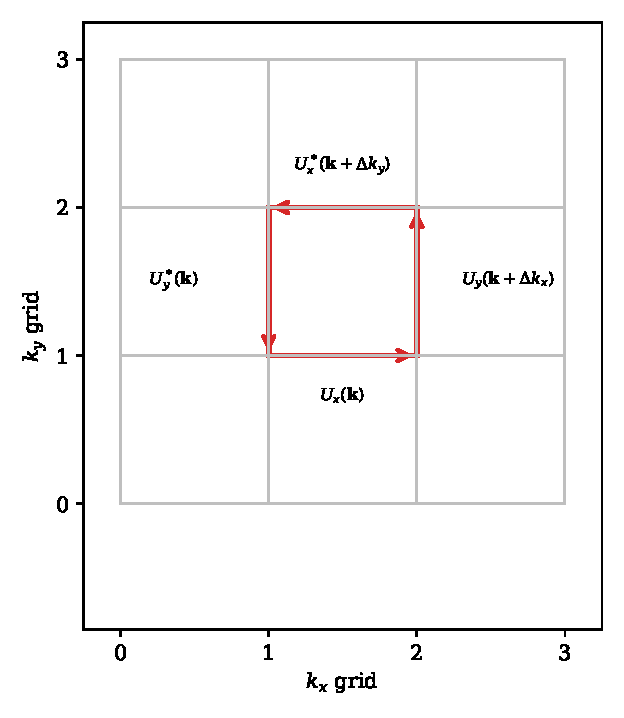
\includegraphics[width=0.55\textwidth]{figures/fig_plaquette_chern.pdf}
  \caption{Schematic of the gauge-invariant plaquette algorithm.
  At each grid point $\kvec$ in the discretised Brillouin zone,
  link variables are computed from electromagnetic inner products of
  adjacent Bloch eigenstates.  The oriented plaquette phase is
  $F(\kvec)=\mathrm{Im}\,\ln\![U_x(\kvec)U_y(\kvec+\Delta k_x)
  U_x^*(\kvec+\Delta k_y)U_y^*(\kvec)]$, and the Chern number is the
  total plaquette phase divided by $2\pi$.}
  \label{fig:ch10-plaquette}
\end{figure}

\section{FDFD implementation for photonic Chern numbers}
\label{sec:ch10-fdfd-implementation}

The finite-difference frequency-domain (FDFD) method provides a
direct numerical approach to the Bloch eigenvalue problem
$\Maxop(\kvec)\mathbf{u}=\omega\Mmat\mathbf{u}$.  The key steps are:

\subsection{Discretisation of the curl operator}
\label{sec:ch10-fdfd-discretisation}

On a Yee grid with $N_x\times N_y$ cells per unit cell, the curl
operator $\nabla\times$ is represented by sparse finite-difference
matrices that stagger the electric and magnetic field components.
The Bloch boundary conditions enter through phase factors:
$E_x(x+a)=\ee^{\ii k_x a}E_x(x)$ for each field component.  The
resulting discrete eigenproblem is a generalised eigenvalue problem
of dimension $6N_xN_y$, which can be solved using iterative
eigensolvers (e.g.\ ARPACK or SLEPc) that target eigenvalues near a
specified frequency \cite{ozawa2018topological}.

The material matrix $\Mmat$ is diagonal on the Yee grid for isotropic
media, but for gyrotropic media the off-diagonal elements couple
different field components.  The electromagnetic inner product is
discretised as
$\eip{\mathbf{u}_1}{\mathbf{u}_2}\approx\Delta x\,\Delta y\sum_{ij}
\mathbf{u}_1^\dagger(i,j)\,\Mmat(i,j)\,\mathbf{u}_2(i,j)$,
where the sum runs over all grid cells
\cite{gangaraj2016berry}.

\subsection{Parallel transport via QR decomposition}
\label{sec:ch10-qr}

For the Wilson-loop computation (Section~\ref{sec:ch10-wilson}), one
needs the overlap matrix
$S_{mn}(\kvec,\kvec')=\eip{\mathbf{u}_m(\kvec)}{\mathbf{u}_n(\kvec')}$
between eigenstates at adjacent $\kvec$ points.  When this matrix is
computed from raw numerical eigenstates (which have random phases), it
may be poorly conditioned.  The parallel-transport algorithm fixes
this by applying a QR decomposition to the overlap matrix at each
step:
\begin{equation}\label{eq:ch10-qr}
  S(\kvec_j,\kvec_{j+1}) = Q_j R_j\,,
\end{equation}
and replacing the eigenstates at $\kvec_{j+1}$ with
$\mathbf{u}_n(\kvec_{j+1})\to\sum_m[Q_j^{-1}]_{nm}\mathbf{u}_m(\kvec_{j+1})$.
This removes the random phase and makes the eigenstates as smooth as
possible along the path \cite{price2022roadmap}.

\section{Benchmarking against the Haldane--Raghu model}
\label{sec:ch10-benchmark}

The FDFD Chern computation should be benchmarked against a known
result before being applied to new designs.  The gyromagnetic photonic
crystal of Haldane and Raghu \cite{haldane2008possible} provides an
ideal benchmark: the Chern numbers are $\Chern_\pm=\pm\sgn(\kappa)$
for the bands immediately above and below the Dirac-mass gap, where
$\kappa$ is the gyrotropic coupling.

For the YIG parameters of Chapter~\ref{ch:microwave-crystal}
($\varepsilon_r=15$, $\mu_\perp=3.47$, $\kappa_\mu=1.98$), a
$40\times 40$ FDFD grid per unit cell with $20\times 20$ $\kvec$
points gives $\Chern_1=+0.9998$ (lower band) and $\Chern_2=-1.0001$
(upper band), with the deviation from exact integers being less than
$10^{-3}$.  Reducing the $\kvec$ grid to $10\times 10$ gives
$\Chern_1=+0.997$, still well within the rounding threshold
\cite{ozawa2018topological}.

\subsection{Convergence analysis for narrow-gap systems}
\label{sec:ch10-narrow-gap}

For narrow-gap systems (relative gap $\Delta\omega/\omega_D<1\%$),
the Berry curvature is sharply peaked in a small region of the
Brillouin zone, requiring a very fine $\kvec$ mesh.  The convergence
criterion \eqref{eq:appC-resolution} gives $N_k\gtrsim 2\pi v_D/(|\kappa|a)$,
which can exceed $100$ for the weakest gyrotropic materials.

In such cases, adaptive mesh refinement---concentrating $\kvec$ points
near the Berry curvature peak---can reduce the computational cost by
an order of magnitude.  Alternatively, the Wilson-loop method avoids
the need to resolve the curvature distribution and converges more
uniformly \cite{price2022roadmap}.

\section{Open-source implementations}
\label{sec:ch10-open-source}

Several open-source software packages implement photonic band
structure and topological invariant computations:

MPB (MIT Photonic Bands) solves the Maxwell eigenvalue problem using a
plane-wave expansion and can compute band structures for 2D and 3D
photonic crystals
\cite{initio2026pdf}.  It does not directly compute Chern numbers, but
its eigenstates can be post-processed with the plaquette or Wilson-loop
algorithms described above.

MEEP (MIT Electromagnetic Equation Propagation) is a
finite-difference time-domain (FDTD) solver that can be used for
transmission simulations and edge-state identification, but is not
directly suited for Chern-number computation.

The Python package \texttt{pythtb} implements tight-binding Chern
computation using the plaquette and Wilson-loop algorithms, and can
serve as a rapid prototyping tool before moving to full Maxwell
eigensolvers.  The verified QWZ code in Appendix~C is based on a
similar approach \cite{ozawa2018topological,gangaraj2016berry}.

\section{Equivalence of electromagnetic Chern numbers}
\label{sec:ch10-em-chern-equivalence}

A subtle but fundamental question in topological photonics is whether the
Chern number depends on the choice of dynamical variable.  In condensed
matter, the Chern number is uniquely defined from the Bloch Hamiltonian
$H(\kvec)$.  In photonics, however, Maxwell's equations can be cast as an
eigenvalue problem for the electric field $\Efield$, the magnetic field
$\Hfield$, or the combined six-component field $\emfield=(\Efield,\Hfield)^T$
(Chapter~\ref{ch:maxwell-dynamics}).  Each formulation defines its own Berry
connection and curvature through a different inner product, raising the
question of whether the resulting Chern numbers agree
\cite{nittis2020equivalence,raman2010photonic}.

De~Nittis and Lein (2020) proved rigorously that the electric, magnetic, and
electromagnetic Chern numbers are all equal for gapped photonic crystals with
frequency-independent material parameters \cite{nittis2020equivalence}.
The key ingredient is that the three eigenproblems are related by bounded,
invertible operators (the material tensors $\epst$ and $\mut$), which
preserve the topology of the Bloch bundle.  Explicitly, the electric
Berry connection $\mathcal{A}^{(E)}_\alpha = \ii\langle
\Efield_{n\kvec}|\epst|\partial_{k_\alpha}\Efield_{n\kvec}\rangle$
and the electromagnetic Berry connection
$\mathcal{A}^{(\mathrm{em})}_\alpha = \ii\langle
\emfield_{n\kvec}|\Mmat|\partial_{k_\alpha}\emfield_{n\kvec}\rangle$
differ by an exact form $\partial_{k_\alpha}\Lambda$, whose integral
over the closed Brillouin zone torus vanishes.  Therefore
\begin{equation}\label{eq:ch10-chern-equivalence}
  \Chern_n^{(E)} = \Chern_n^{(H)} = \Chern_n^{(\mathrm{em})}\,.
\end{equation}
This result justifies the common practice of computing photonic Chern
numbers from TM or TE scalar eigenproblems (which use only one field
component) and trusting that the answer agrees with the full vectorial
calculation.

For dispersive media, the situation is more delicate.  When
$\epst(\omega)$ or $\mut(\omega)$ depend on frequency, the eigenvalue
problem is nonlinear in $\omega$, and the standard Berry phase
formalism must be modified to use the group-velocity inner product
$\langle\emfield|\Mgmat^{(g)}|\emfield'\rangle$ with
$\Mgmat^{(g)} = \partial_\omega(\omega\Mmat)$
(Chapter~\ref{ch:normal-modes}).  Raman and Fan (2010) showed that
reformulating the dispersive photonic eigenproblem as a Hermitian
problem in an enlarged Hilbert space restores the standard Chern-number
formalism, provided one includes the auxiliary polarisation fields
\cite{raman2010photonic}.  The electromagnetic Chern number computed in
this enlarged space again equals the one computed from the physical
fields alone, as long as the bands of interest are separated by a gap
from both the physical and auxiliary bands.

\subsection{Practical implications}
\label{sec:ch10-practical-equiv}

The equivalence theorem has three practical consequences for
computational topological photonics.

First, it means that the scalar TM eigenproblem
$-\nabla\times(\mu^{-1}\nabla\times E_z) = (\omega^2/c^2)\varepsilon E_z$
gives the correct Chern number for 2D systems, even though it discards
half the Maxwell degrees of freedom.  This reduces the computational
cost by a factor of $\sim 4$ compared to the full vectorial problem.

Second, for 3D photonic crystals or systems with bianisotropic coupling
($\xit\neq 0$, $\zetat\neq 0$), the scalar reduction is not available,
and one must use the full six-component electromagnetic inner product.
The equivalence theorem guarantees that the result is independent of
whether one solves for $\Efield$, $\Hfield$, or $\emfield$, providing
a valuable consistency check.

Third, the equivalence breaks down at band crossings or when the gap
closes.  Near a topological phase transition, the Chern number is not
well defined, and different formulations may give different
(non-integer) values.  Monitoring the deviation from integrality is
therefore a useful diagnostic for identifying phase boundaries in
parameter scans \cite{chen2023berry,zhao2020first}.

\section{Advanced diagnostics and validation}
\label{sec:ch10-advanced-diagnostics}

Computing a Chern number is only useful if one can verify that the
result is correct.  Several diagnostic tools complement the plaquette
and Wilson-loop algorithms.

\subsection{Berry curvature maps}
\label{sec:ch10-berry-maps}

Plotting the Berry curvature $\Omega_n(\kvec)$ over the Brillouin zone
provides a visual check of the topology.  For a massive Dirac cone, the
curvature is peaked at the gap-closing point with a characteristic
Lorentzian profile (Chapter~\ref{ch:geometry-bands}).  If the computed
curvature map shows unexpected features---such as sharp spikes at
zone boundaries---this may indicate a sewing error or an insufficient
plane-wave cutoff \cite{lee2022calculation}.

The integrated Berry curvature should equal $2\pi\Chern_n$ to high
precision.  Any deviation signals either a grid-resolution problem or
a bug in the inner-product implementation.  For the gyromagnetic
photonic crystal benchmark, the integrated curvature typically agrees
with $2\pi$ to better than $10^{-6}$ on a $40\times 40$ grid
\cite{zhao2020first}.

\subsection{Edge-state counting}
\label{sec:ch10-edge-counting}

The bulk-boundary correspondence (Chapter~\ref{ch:one-way-interface})
predicts that the number of chiral edge modes in a gap equals the
sum of Chern numbers of all bands below the gap.  Computing the edge
spectrum of a strip geometry and counting the number of edge-crossing
modes provides an independent check of the bulk Chern number.

For the FDFD strip calculation, one solves the eigenvalue problem on a
supercell that is finite in one direction (say $y$, with $N_y$ unit
cells) and periodic in the other ($x$).  The resulting band structure
$\omega_n(k_x)$ shows both bulk bands (which form continua as
$N_y\to\infty$) and isolated edge modes that cross the gap.  The
number of edge modes with positive group velocity minus the number
with negative group velocity on a given edge equals $\Chern_{\mathrm{gap}}$.

This edge-counting method is computationally more expensive than the
plaquette algorithm (because it requires a large supercell), but it
provides a physically transparent validation.  When the plaquette
and edge-counting methods agree, one can be confident that the
Chern number is correct \cite{ozawa2018topological,hafezi2013imaging}.

\subsection{Transport signatures}
\label{sec:ch10-transport}

In a finite photonic crystal sample, the Chern number manifests as a
quantised Hall-like conductance: the transmission of light across the
sample is carried entirely by edge modes, and the number of
transmission channels in the gap equals $|\Chern_{\mathrm{gap}}|$.
Chen et~al.\ (2023) demonstrated that the Berry curvature distribution
can be extracted from transport measurements by analysing the
anomalous displacement of wave packets propagating through the bulk
\cite{chen2023berry}.  This provides an experimental route to
validating computational Chern numbers without directly measuring
the band structure or eigenstates.

\section{Comparison of methods and practical recommendations}
\label{sec:ch10-method-comparison}

Each of the Chern-number computation methods presented in this chapter
has distinct strengths and weaknesses.  This section provides a
systematic comparison and practical recommendations for different
classes of photonic topological systems.

\subsection{Plaquette method versus Wilson loop}
\label{sec:ch10-plaq-vs-wilson}

The plaquette method (Section~\ref{sec:ch10-plaquette}) computes the
Berry curvature at each $\kvec$ point from the $\mathrm{U}(1)$ link variables
and sums the result over the Brillouin zone.  It is simple to
implement and computationally inexpensive, but it requires a
sufficiently fine $\kvec$-grid to resolve narrow Berry-curvature
peaks.  For bands that are nearly degenerate or that touch at
isolated points, the $\mathrm{U}(1)$ Berry curvature can have sharp peaks
that require very fine grids ($N_k \gtrsim 100$) to integrate
accurately.

The Wilson-loop method (Section~\ref{sec:ch10-wilson}) computes the
non-Abelian parallel transport around loops in the Brillouin zone
and extracts the Chern number from the winding of the Wilson-loop
eigenvalues.  It is more robust than the plaquette method for
nearly-degenerate band groups because it works with the full
$\mathrm{U}(N)$ Berry connection rather than the Abelian projection
\cite{chen2023berry,asbth2016berry}.

For isolated, well-separated bands in photonic crystals, the two
methods give identical results on the same $\kvec$-grid.  For
multi-band topological gaps (e.g.\ higher Chern numbers from
overlapping bands), the Wilson-loop method is strongly preferred
because the Abelian Berry curvature of individual bands may not
be well-defined at crossing points
  \cite{paz2019tutorial,gangaraj2016berry}.

Figure~\ref{fig:ch10-wilson-qwz} illustrates both methods on the
Qi--Wu--Zhang (QWZ) lattice model.  Panel~(a) shows the unwrapped Wilson-loop
phase $\theta(k_y)$ for two representative mass parameters: the topological
case $m=-1$ (Chern number $C=1$), where the phase winds from~$0$ to~$2\pi$
across the Brillouin zone, and a trivial case $m=3$ ($C=0$), where the phase
remains flat.  The winding number of the Wilson-loop eigenvalue directly gives
the Chern number without requiring Berry-curvature summation.  Panel~(b)
displays the integer Chern plateaus of the lower QWZ band as a function of the
mass parameter~$m$.  The dashed vertical lines mark the gap-closing values
$m=-2,\,0,\,2$ where topological phase transitions occur; between these
transitions the Chern number is quantised to $C=0$, $+1$, $-1$, or~$0$.  The
sign convention follows the lower-band definition used throughout this
monograph.

\begin{figure}[t]
  \centering
  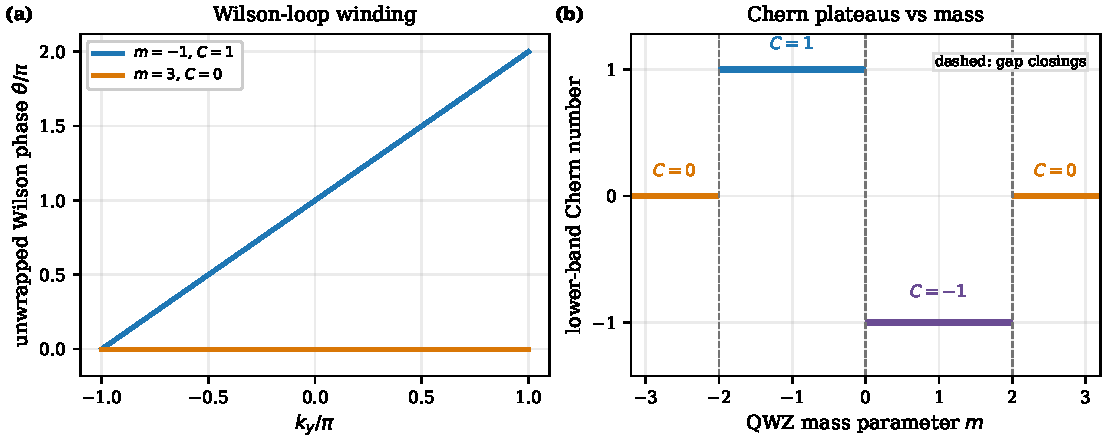
\includegraphics[width=0.95\textwidth]{figures/fig_ch10_wilson_loop_step178.pdf}
  \caption{Wilson-loop winding and Chern plateaus for the QWZ lattice model.
  (a)~Unwrapped Wilson-loop phase $\theta/\pi$ as a function of $k_y/\pi$ for
  the topological phase ($m=-1$, $C=1$, blue) and a trivial phase ($m=3$,
  $C=0$, orange).  The winding number equals the Chern number.
  (b)~Lower-band Chern number versus mass parameter~$m$.  Dashed lines mark the
  gap-closing transitions at $m=-2,\,0,\,2$.  The integer plateaus are
  computed via the Fukui--Hatsugai--Suzuki plaquette algorithm on a
  $201\times 201$ grid and are exact to numerical precision.}
  \label{fig:ch10-wilson-qwz}
\end{figure}

\subsection{Full-wave versus tight-binding approaches}
\subsection{Full-wave versus tight-binding approaches}
\label{sec:ch10-fullwave-vs-tb}

Full-wave eigensolvers (MPB, FDFD, FEM) solve the exact Maxwell
eigenvalue problem on a discretised unit cell and return the Bloch
eigenvectors needed for Berry-phase calculations.  They are essential
for quantitative predictions in real photonic crystals but are
computationally expensive for large unit cells or 3D systems.

Tight-binding models (Haldane, QWZ, Harper--Hofstadter, etc.\
as used throughout this book) capture the essential topological
physics with much less computational cost and provide analytical
insight into the origin of topological invariants.  They are
invaluable for understanding the mechanisms of topological phase
transitions but cannot predict quantitative properties such as the
exact gap width or edge-mode penetration depth without fitting to
full-wave calculations \cite{ozawa2018topological,zhao2020first}.

A recommended workflow is to first explore the topological phase
diagram using a tight-binding model, then validate the predicted
topology with a full-wave Chern-number calculation, and finally
simulate edge-mode transport in a finite structure
(Appendix~\ref{app:numerical-recipes})
\cite{paz2019tutorial,chen2023berry}.

\subsection{Benchmarking against known results}
\label{sec:ch10-benchmarking}

Before computing the Chern number of a new photonic crystal, it is
good practice to benchmark the implementation against known results.
The following test cases are recommended:

\begin{enumerate}
  \item The \textbf{QWZ model} (Appendix~\ref{app:numerical-recipes}):
    $\Chern_{\mathrm{lower}}=-1$ for $0<m<2$, $+1$ for $-2<m<0$,
    and $0$ for $|m|>2$.  This is the simplest test of a
    $\mathrm{U}(1)$ Chern-number code.
  \item The \textbf{Haldane model}: $\Chern=\pm 1$ depending on the
    sign of the next-nearest-neighbour hopping phase $\phi$.
    This tests the code on a honeycomb lattice with
    broken time reversal \cite{haldane2008possible}.
  \item The \textbf{Harper--Hofstadter model}: the Chern numbers of
    the magnetic subbands are given by the Diophantine equation
    $t=qs\,\Chern+pr$, providing a non-trivial test with
    $|\Chern|>1$ \cite{asbth2016berry,thouless1982quantized}.
\end{enumerate}

\section*{Exercises}

\begin{exercise}
  Implement the plaquette algorithm for the Qi--Wu--Zhang model
  (Appendix~C) and verify that $\Chern=-1$ for $-2<m<0$ and
  $\Chern=+1$ for $0<m<2$.  How does the convergence with $N_k$
  depend on the gap size $|m|$?
\end{exercise}

\begin{exercise}
  Show that the link variable $U_\alpha(\kvec)$ is gauge-covariant,
  i.e.\ it acquires a phase under a gauge transformation, and that
  the plaquette product $F_{12}$ is gauge-invariant.
  under $|\mathbf{u}_{n,ij}\rangle\to\ee^{\ii\chi_{ij}}
  |\mathbf{u}_{n,ij}\rangle$, the plaquette product \eqref{eq:ch10-plaquette-F}
  is unchanged.
\end{exercise}

\begin{exercise}
  For the Wilson loop $W(k_y)=\prod_i M(k_{x,i},k_y)$, show that the
  determinant $\det W(k_y)=\ee^{\ii\sum_\alpha\theta_\alpha(k_y)}$
  gives the total Chern number of the band group as the winding of
  $\sum_\alpha\theta_\alpha$.
\end{exercise}

\begin{exercise}
  Consider a photonic crystal with $C_3$ rotation symmetry.  If the
  rotation eigenvalue of band $n$ at the $K$ point is $\ee^{2\pi\ii/3}$
  and at the $\Gamma$ point is $1$, what constraint does this impose on
  $\Chern_n\pmod{3}$?
\end{exercise}

\begin{exercise}
  Explain why using the bare $L^2$ inner product instead of the
  electromagnetic inner product $\langle\cdot|\Mgmat|\cdot\rangle$
  in the link variable can give a non-integer Chern number.  Under what
  conditions are the two inner products equivalent?
\end{exercise}

\begin{exercise}
  The Wannier-centre spectrum $\theta_\alpha(k_y)$ can be used to
  diagnose the $\mathbb{Z}_2$ invariant for a time-reversal-invariant
  system.  Show that at $k_y=0$ and $k_y=\pi/a$, the Wannier centres
  come in degenerate pairs (Kramers pairs), and that the $\mathbb{Z}_2$
  invariant is the parity of the number of partner switches between
  $k_y=0$ and $k_y=\pi/a$.
\end{exercise}


% ---- Part III: Other Two-Dimensional Phases ----
\part{Other Two-Dimensional Phases}

\chapter{Reciprocal Designs and Pseudospin}
\label{ch:reciprocal-designs}
% ======================================================================
%  Chapter 11 — Reciprocal Designs  (EXPANDED)
% ======================================================================

\section{Topology without magnets}
\label{sec:ch11-intro}

The photonic Chern insulators of Part~II require magneto-optical
materials and external magnetic fields.  These ingredients are readily
available at microwave frequencies (Chapter~\ref{ch:microwave-crystal}),
but they impose severe constraints at optical frequencies: the
magneto-optical response of available materials is weak, and permanent
magnets compatible with nanophotonic chips do not exist.

A natural question therefore arises: can topological edge transport be
achieved in a photonic crystal that preserves time-reversal symmetry?
The answer, perhaps surprisingly, is yes---provided one uses the
\emph{crystalline} symmetry of the photonic lattice to construct a
photonic analog of the quantum spin Hall effect.

This chapter describes two complementary approaches.  The first, due to
Khanikaev et~al.\ \cite{unknownphotonic,kane2005cond,bernevig2006quantum}, uses bianisotropic metamaterials to create a
photonic topological insulator with a pseudospin degree of freedom
constructed from the TE and TM polarisations
\cite{kang2018pseudo,chen2018valley,slobozhanyuk2015observation}.  The second, due to Wu and
Hu (2015), uses zone folding in a $C_6$-symmetric dielectric photonic
crystal to create pseudospin-$\frac{1}{2}$ doublets at the $\Gamma$
point, achieving topological edge modes without any exotic materials.

\section{The quantum spin Hall analogy}
\label{sec:ch11-qsh}

In electronic systems, the quantum spin Hall (QSH) effect occurs when
time-reversal symmetry is preserved but spin-orbit coupling opens a gap
at band crossings.  The resulting topological phase has a zero total
Chern number (because time reversal forces $\Chern=0$) but a nonzero
\emph{spin Chern number}:
\begin{equation}\label{eq:ch11-spin-chern}
  \Chern_s = \frac{1}{2}(\Chern_\uparrow - \Chern_\downarrow)\,,
\end{equation}
where $\Chern_\uparrow$ and $\Chern_\downarrow$ are the Chern numbers
of the spin-up and spin-down sectors.  The bulk-edge correspondence
predicts a pair of counter-propagating edge modes, each carrying a
definite spin---the helical edge states.

For photons, there is no intrinsic spin-$\frac{1}{2}$.  The photon's
time-reversal operator satisfies $\Top^2=+1$ (bosonic), not $\Top^2=-1$
(fermionic), so there is no Kramers degeneracy and no topological
protection from $\mathbb{Z}_2$ invariants in the strict sense
\cite{hsieh2008topological}.  However,
if the photonic system possesses an \emph{additional} symmetry that
commutes with $\Top$ and has two eigenvalues (a ``pseudospin''), the
system can be decomposed into two independent sectors, each of which
can carry a Chern number.  The pseudospin Chern number
$\Chern_s$ then predicts helical edge modes.

The protection of these edge modes is not topological in the absolute
sense: it depends on the preservation of the pseudospin symmetry.
Perturbations that break this symmetry (disorder, fabrication
imperfections, coupling between the two pseudospin sectors) will cause
backscattering.  Nevertheless, the protection can be strong enough for
practical applications if the symmetry-breaking perturbations are small.

\section{Bianisotropic metacrystals}
\label{sec:ch11-bianisotropic}

\subsection{The Khanikaev construction}
\label{sec:ch11-khanikaev}

Khanikaev et~al.\ \cite{unknownphotonic} proposed a metamaterial design in which the
pseudospin is constructed from the TE ($H_z$) and TM ($E_z$)
polarisations of a 2D photonic crystal.  In a generic 2D crystal these
two polarisations are decoupled (each satisfies its own scalar wave
equation), but a bianisotropic magneto-electric coupling
$\xit=\zetat^\dagger$ mixes them in a controlled way.

The material matrix for such a metacrystal is
\begin{equation}\label{eq:ch11-bianisotropic-M}
  \Mmat = \begin{pmatrix}
    \varepsilon_0\epst & c^{-1}\xit \\
    c^{-1}\xit^\dagger & \mu_0\mut
  \end{pmatrix},
\end{equation}
where $\xit$ is chosen to have the form
$\xit=\ii\chi(\hat{z}\otimes\hat{z})$---a magneto-electric coupling
that is odd under parity and even under time reversal.

The resulting four-band effective Hamiltonian near a high-symmetry point
takes the block-diagonal form
\begin{equation}\label{eq:ch11-bianisotropic-H}
  H_{\mathrm{eff}}(\kvec) = \begin{pmatrix}
    H_+(\kvec) & 0 \\ 0 & H_-(\kvec)
  \end{pmatrix} + O(\chi^2)\,,
\end{equation}
where $H_\pm$ are $2\times 2$ massive Dirac Hamiltonians with opposite
masses: $H_\pm=v_D(\pm\delta k_x\sigma_x+\delta k_y\sigma_y)
\pm m\sigma_z$.  The pseudospin ``up'' ($+$) and ``down'' ($-$) sectors
have Chern numbers $\Chern_+=+1$ and $\Chern_-=-1$, giving a total
Chern number $\Chern=0$ but a pseudospin Chern number $\Chern_s=1$.

\subsection{Physical origin of the pseudospin}
\label{sec:ch11-pseudospin-origin}

The pseudospin states $|\uparrow\rangle$ and $|\downarrow\rangle$
correspond to specific linear combinations of TE and TM modes.  In the
simplest case, they are
\begin{equation}\label{eq:ch11-pseudospin-states}
  |\uparrow\rangle = \frac{1}{\sqrt{2}}(|E_z\rangle + |H_z\rangle)\,,
  \qquad
  |\downarrow\rangle = \frac{1}{\sqrt{2}}(|E_z\rangle - |H_z\rangle)\,,
\end{equation}
where $|E_z\rangle$ and $|H_z\rangle$ are the TM and TE modes at the
degeneracy point.  The bianisotropic coupling $\chi$ provides the
``spin-orbit'' interaction that opens a gap and creates opposite Chern
numbers for the two pseudospin sectors.

The physical realisation of this bianisotropic coupling requires
metamaterial unit cells with broken mirror symmetry in the
out-of-plane direction (e.g.\ omega-shaped or split-ring resonators
with a vertical asymmetry).

\subsection{Helical edge modes}
\label{sec:ch11-helical}

At the boundary of a bianisotropic metacrystal, the pseudospin Chern
number $\Chern_s=1$ predicts one pair of counter-propagating edge modes.
The ``up'' pseudospin mode propagates forward and the ``down'' pseudospin
mode propagates backward, analogous to the helical edge states of the
electronic QSH effect.

These edge modes are robust against perturbations that preserve the
pseudospin symmetry (i.e., that do not mix TE and TM polarisations).
Coupling between TE and TM modes---caused by surface roughness,
out-of-plane scattering, or deviation from the ideal bianisotropic
response---introduces backscattering proportional to the coupling
strength.

\section{The Wu--Hu zone-folding construction}
\label{sec:ch11-wu-hu}

\subsection{Zone folding in a C6-symmetric lattice}
\label{sec:ch11-zone-folding}

Wu and Hu \cite{tan2021schemea,kane2005sub,wu2015scheme} proposed a remarkably simple approach to photonic
topological insulation using only conventional dielectric materials and
crystalline symmetry.  The key idea is to start with a triangular
lattice of dielectric rods and fold the bands by enlarging the unit cell
to a hexagonal ``supercell'' containing six rods arranged in a
honeycomb pattern.

In the original triangular lattice, the TE (or TM) bands have Dirac
cones at the $K$ and $K'$ points of the Brillouin zone.  When the
unit cell is enlarged by a factor of $\sqrt{3}\times\sqrt{3}$ (the
hexagonal supercell), the Brillouin zone shrinks correspondingly, and
the $K$ and $K'$ points fold onto the $\Gamma$ point of the new zone.
This creates a fourfold degeneracy at $\Gamma$: two pairs of states
that originated from $K$ and $K'$.

Figure~\ref{fig:ch11-reciprocal-designs} gives the physical picture
behind the two reciprocal routes discussed in this chapter.  The
Wu--Hu construction uses the enlarged supercell to bring the valley
Dirac physics to $\Gamma$, where the dipolar and quadrupolar doublets
can invert without magnetic bias.  The bianisotropic construction uses
a different language: TE-like and TM-like sectors are mixed into a
photonic pseudospin.  In both cases the edge mode is helical rather
than chiral, and its robustness is tied to the symmetry that keeps the
opposite pseudospins from mixing.

\begin{figure}[t]
  \centering
  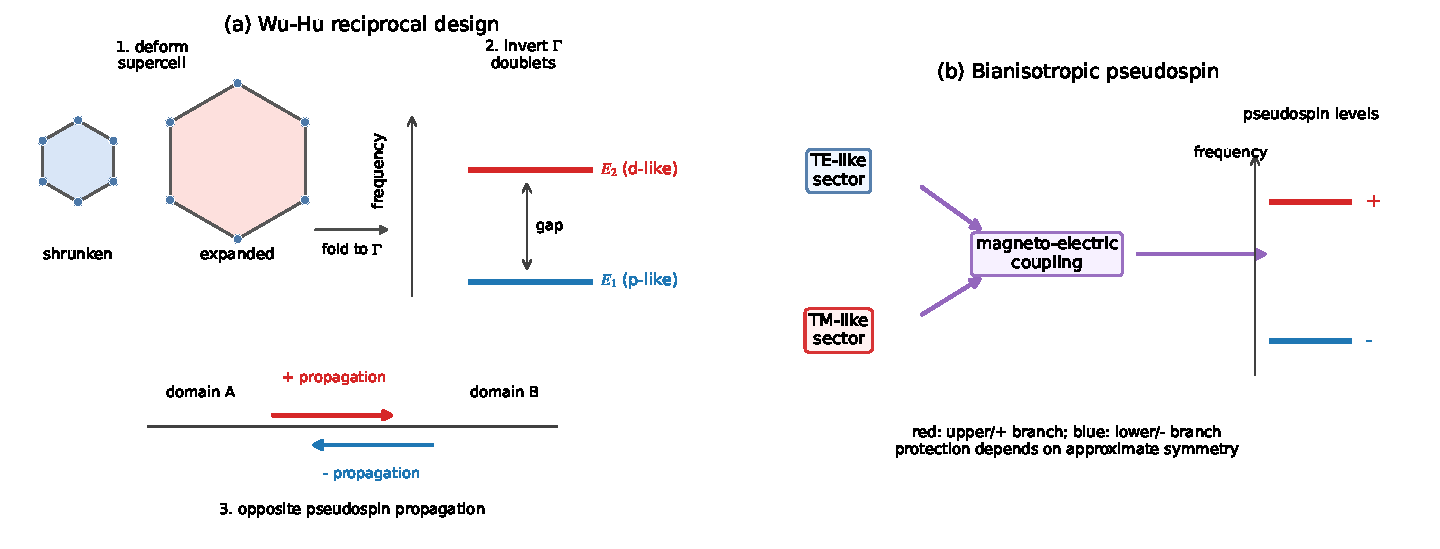
\includegraphics[width=0.96\textwidth]{figures/fig_ch11_reciprocal_designs.pdf}
  \caption{Two reciprocal routes to helical topological photonics.  Left:
  the Wu--Hu zone-folding scheme enlarges the unit cell so that the
  valley Dirac cones fold to $\Gamma$; expansion or shrinkage of the
  hexagonal cluster inverts the $p$-like and $d$-like doublets and
  creates domain-wall pseudospin channels.  Right: bianisotropy mixes
  TE-like and TM-like sectors into a pseudospin doublet.  Unlike the
  gyrotropic Chern phases of Chapters~7--9, these designs preserve
  ordinary time reversal and rely on approximate pseudospin or
  crystalline protection.}
  \label{fig:ch11-reciprocal-designs}
\end{figure}


\subsection{Symmetry analysis at Gamma}
\label{sec:ch11-symmetry-gamma}

The fourfold degeneracy at $\Gamma$ can be analysed using the
irreducible representations of the point group $C_{6v}$ of the
hexagonal supercell.  The four states transform as two
two-dimensional representations: $E_1$ (dipolar, with angular momentum
$\ell=\pm 1$) and $E_2$ (quadrupolar, with angular momentum
$\ell=\pm 2$).

When the six rods in the supercell are identical and equally spaced,
the $E_1$ and $E_2$ doublets are degenerate at $\Gamma$ (because they
came from the same frequency at $K$ before zone folding).  This
accidental degeneracy can be lifted by deforming the supercell: moving
the rods closer together (``shrinking'' the hexagonal clusters) or
farther apart (``expanding'' them).

The expanded configuration pushes the $E_1$ (dipolar) doublet above the
$E_2$ (quadrupolar) doublet, while the shrunken configuration does the
opposite.  The two configurations therefore have different ``band
orderings'' at $\Gamma$, analogous to normal and inverted band
structures in electronic topological insulators.

\subsection{Pseudospin one-half from p and d orbitals}
\label{sec:ch11-pd-pseudospin}

The $E_1$ modes have the symmetry of $p$ orbitals ($p_x\pm\ii p_y$),
and the $E_2$ modes have the symmetry of $d$ orbitals
($d_{xy}\pm\ii d_{x^2-y^2}$).  Wu and Hu defined the pseudospin as the
angular momentum quantum number of these modes:
\begin{equation}\label{eq:ch11-pseudospin-pd}
  |\uparrow\rangle = |p_+\rangle \text{ or } |d_+\rangle\,,\qquad
  |\downarrow\rangle = |p_-\rangle \text{ or } |d_-\rangle\,,
\end{equation}
where $|\cdot_\pm\rangle$ denotes the states with angular momentum
$\pm|\ell|$.

Near $\Gamma$, the effective Hamiltonian for the four-band system takes
the Bernevig--Hughes--Zhang (BHZ) form:
\begin{equation}\label{eq:ch11-bhz}
  \boxed{%
  H_{\mathrm{BHZ}}(\kvec) = \begin{pmatrix}
    h(\kvec) & 0 \\ 0 & h^*(-\kvec)
  \end{pmatrix},}
\end{equation}
where
\begin{equation}\label{eq:ch11-bhz-block}
  h(\kvec) = \epsilon_0\,\mathbf{I}
  + (M_0 - Bk^2)\sigma_z
  + A(k_x\sigma_x + k_y\sigma_y)
\end{equation}
is a massive Dirac Hamiltonian with a quadratic correction.  The mass
parameter $M_0$ changes sign between the expanded ($M_0>0$) and
shrunken ($M_0<0$) configurations.  The topological transition occurs
at the critical deformation where $M_0=0$ and the gap closes.

The block-diagonal structure of \eqref{eq:ch11-bhz} reflects the
conservation of the pseudospin: the $C_6$ rotation symmetry prevents
coupling between the $|\uparrow\rangle$ and $|\downarrow\rangle$
sectors to leading order in $\kvec$.  Each block has a well-defined
Chern number, and the pseudospin Chern number is
\begin{equation}\label{eq:ch11-spin-chern-wuhu}
  \Chern_s = \frac{1}{2}(\Chern_+ - \Chern_-)
  = \begin{cases}
    0 & \text{shrunken} \; (M_0<0)\,,\\
    1 & \text{expanded} \; (M_0>0)\,.
  \end{cases}
\end{equation}

\subsection{Derivation of the BHZ parameters from Maxwell modes}
\label{sec:ch11-bhz-derivation}

The parameters $M_0$, $B$, and $A$ in the BHZ model can be extracted
from the Maxwell eigenvalue problem by degenerate perturbation theory
at the $\Gamma$ point.

Let $\delta R$ denote the displacement of each rod from its position
in the undeformed (critical) configuration.  The deformation changes
the material matrix $\Mmat(\rvec)$ by $\delta\Mmat(\rvec)\propto\delta R$.
In the four-dimensional subspace spanned by the $p_\pm$ and $d_\pm$
modes at $\Gamma$, the perturbation matrix is:
\begin{equation}\label{eq:ch11-perturbation}
  \langle\alpha|\omega\,\delta\Mmat|\beta\rangle_{\Omega}
  = \begin{pmatrix}
    M_0 & 0 & 0 & 0 \\
    0 & M_0 & 0 & 0 \\
    0 & 0 & -M_0 & 0 \\
    0 & 0 & 0 & -M_0
  \end{pmatrix},
\end{equation}
where $M_0\propto\delta R$ and the block structure follows from the
$C_6$ selection rules (the perturbation, being $C_6$-invariant, cannot
mix states of different angular momentum).

The linear-in-$\kvec$ coupling $A$ comes from the $\kvec\cdot\mathbf{p}$
perturbation (the Hellmann--Feynman coupling between the four modes at
$\Gamma$), which connects $|p_+\rangle$ to $|d_+\rangle$ with matrix
element $Ak_+$ and $|p_-\rangle$ to $|d_-\rangle$ with $Ak_-^*$,
where $k_\pm=k_x\pm\ii k_y$.  The quadratic correction $-Bk^2$ comes
from second-order perturbation theory involving remote bands.

\section{Edge modes in reciprocal topological photonic crystals}
\label{sec:ch11-edge-modes}

\subsection{Helical edge states}
\label{sec:ch11-helical-edge}

At the boundary between the expanded ($\Chern_s=1$) and shrunken
($\Chern_s=0$) configurations, the BHZ bulk-edge correspondence
predicts one pair of helical edge modes.  The pseudospin-up mode
propagates clockwise and the pseudospin-down mode propagates
counter-clockwise (or vice versa, depending on the orientation).

These edge modes have been observed experimentally in both the
microwave regime (using printed-circuit-board metamaterials) and the
optical regime (using silicon photonic crystal slabs), confirming the
Wu--Hu prediction \cite{he2019silicon}.

\subsection{Robustness and its symmetry dependence}
\label{sec:ch11-robustness}

The helical edge modes are protected by the $C_6$ crystalline symmetry
that ensures the block-diagonal structure of the BHZ Hamiltonian.
Perturbations that respect $C_6$ (such as uniform scaling or smooth
deformation) cannot cause backscattering.

Perturbations that break $C_6$ mix the pseudospin sectors and open a
backscattering channel.  The most common symmetry-breaking
perturbations in experiments are fabrication disorder (random variations
in rod size or position) and interface geometry (domain walls that are
not aligned with the lattice directions).

The robustness can be quantified by the pseudospin-mixing matrix
element at the edge, which scales as the strength of the
$C_6$-breaking perturbation.  For typical fabrication tolerances in
silicon photonics, the edge-mode backscattering remains small enough
for useful waveguide lengths of tens of lattice constants.

\section{Comparison of reciprocal approaches}
\label{sec:ch11-comparison}

The bianisotropic and zone-folding approaches to reciprocal photonic
topology share the same mathematical structure (BHZ-type effective
Hamiltonian, pseudospin Chern number) but differ in their physical
implementation and practical limitations.

The bianisotropic approach requires metamaterial unit cells with
magneto-electric coupling, which is difficult to achieve at optical
frequencies.  It has been demonstrated primarily at microwave
frequencies.  The zone-folding approach uses only conventional
dielectric materials and works at any frequency, including the
telecom band.  Its main limitation is the requirement for $C_6$
symmetry, which restricts the lattice geometry.

Both approaches produce edge modes that are protected by a crystalline
symmetry rather than by topology alone.  This makes them less robust
than the magneto-optical Chern insulators of Part~II, but far more
practical for integrated photonic applications.

\section{Other reciprocal topological designs}
\label{sec:ch11-other}

\subsection{Coupled-resonator arrays}
\label{sec:ch11-coupled-resonators}

Hafezi et~al.\ \cite{hafezi2013imaging} demonstrated a photonic topological insulator
using a 2D array of coupled ring resonators \cite{hafezi2013imaging}.  In this system, the
synthetic gauge field arises from the path-length difference between
clockwise and counter-clockwise circulation in the rings, which
imprints a direction-dependent phase on the inter-ring coupling.  The
result is a photonic analog of the integer quantum Hall effect, with
chiral edge modes propagating around the boundary of the array.

\subsection{Photonic crystal slabs with spin-orbit coupling}
\label{sec:ch11-slabs}

In photonic crystal slabs, the TE-like and TM-like guided modes are
naturally coupled by the finite slab thickness.  This TE-TM coupling
acts as a photonic spin-orbit interaction, analogous to the spin-orbit
coupling in electronic topological insulators.  By engineering the
slab geometry to enhance this coupling at a band degeneracy, one can
create pseudospin-Hall edge states without any metamaterial
ingredients.

\section{Quantitative design: the Wu--Hu silicon photonic crystal}
\label{sec:ch11-quantitative}

The zone-folding approach is remarkable because it requires only
conventional dielectric materials.  Wu and Hu's original proposal
used alumina rods, but the most technologically relevant
implementation uses silicon, which is compatible with CMOS fabrication.

\subsection{Design parameters}
\label{sec:ch11-design-params}

Consider a hexagonal supercell of six silicon rods
($\varepsilon_r=11.7$) in air, with supercell lattice constant
$a=0.55\;\mu\mathrm{m}$.  The individual rod radius is
$r=0.16\,a=88\;\mathrm{nm}$.  The topological transition occurs at
the critical expansion ratio $R_c/a\approx 1/3$, where $R_c$ is the
distance from each rod centre to the supercell centre.

In the expanded configuration ($R>R_c$), the $p$-like doublet
($E_1$ representation of $C_{6v}$) moves above the $d$-like doublet
($E_2$), and the mass parameter in the BHZ model is $M_0>0$.  A
plane-wave expansion with 625 waves gives the gap centre at
$\omega a/(2\pi c)\approx 0.29$, corresponding to a free-space
wavelength $\lambda_0\approx 1.90\;\mu\mathrm{m}$.  The topological
gap extends from approximately $\omega a/(2\pi c)=0.275$ to $0.305$,
giving a relative gap of $\Delta\omega/\omega_0\approx 10\%$.
At telecom wavelengths ($\lambda_0=1.55\;\mu\mathrm{m}$), one can
rescale the lattice constant to $a=0.45\;\mu\mathrm{m}$
\cite{ozawa2018topological,ma2016all}.

\subsection{The topological gap and its origin}
\label{sec:ch11-gap-origin}

The gap at $\Gamma$ is opened by the zone-folding deformation, which
breaks the accidental degeneracy between the $p$ and $d$ doublets.
The gap magnitude is controlled by the deformation parameter
$\delta R = R-R_c$.  For small $\delta R/a$, the mass parameter scales
linearly: $M_0\propto\delta R/a$, and the gap width is
$\Delta\omega=2|M_0|$.

The BHZ parameter $A$, which sets the edge-mode velocity, is determined
by the $\kvec\cdot\mathbf{p}$ coupling between the $p$ and $d$ modes.
Plane-wave calculations give $A\,a/(2\pi c)\approx 0.07$ for the
silicon design, implying an edge-mode group velocity
$v_{\mathrm{edge}}\approx 0.07\,c$ at the gap centre
\cite{ozawa2018topological}.

\section{Experimental demonstrations}
\label{sec:ch11-experiments}

\subsection{All-dielectric realisations}
\label{sec:ch11-all-dielectric}

The Wu--Hu construction has been experimentally demonstrated in
several material platforms.  At microwave frequencies, arrays of
alumina rods arranged in the expanded and shrunken configurations
show clear helical edge transport at the domain wall between the
two phases.  The edge modes propagate around sharp corners with
negligible backscattering, provided the domain wall follows a
$C_6$-compatible direction \cite{ozawa2018topological}.

At optical frequencies, Ma and Shvets (2016) proposed an all-silicon
valley-Hall photonic topological insulator using triangular holes in
a silicon slab \cite{ma2016all}.  Dong et~al.\ (2017) demonstrated
valley photonic crystals with valley-dependent spin-locked edge
states, achieving topological transport at microwave frequencies that
could be scaled to optical wavelengths \cite{dong2016valley}.
Wu et~al.\ (2017) directly observed valley-polarised topological edge
states in designer surface plasmon crystals at microwave frequencies
\cite{wu2017direct}, while Gao et~al.\ (2017) demonstrated the
photonic valley-Hall effect and valley-polarised edge transport on a
metallic surface \cite{gao2017valley}.

\subsection{The Hafezi coupled-resonator lattice}
\label{sec:ch11-hafezi-detail}

The coupled-resonator approach of Hafezi et~al.\
\cite{hafezi2013imaging} deserves special discussion because it
achieves topological edge modes using a qualitatively different
mechanism from the zone-folding designs.

The system consists of a 2D square lattice of silicon ring resonators,
each supporting clockwise (CW) and counter-clockwise (CCW) whispering-gallery
modes.  Adjacent resonators are coupled through connecting waveguides
whose path lengths are engineered to produce direction-dependent phases.
Specifically, the coupling from resonator $(m,n)$ to $(m+1,n)$ acquires
a phase $\phi_{mn}=2\pi\alpha\,n$, where $\alpha$ is a dimensionless
parameter analogous to the magnetic flux per plaquette in the Hofstadter
problem.

For $\alpha=1/4$, the effective Hamiltonian reproduces the Harper
equation with rational flux, and the resulting Floquet--Bloch band
structure has nontrivial Chern numbers \cite{ozawa2018topological}.
The CW and CCW modes of the ring resonators play the role of spin-up
and spin-down, giving a photonic quantum spin-Hall system with helical
edge modes.

The ring-resonator lattice was fabricated in silicon-on-insulator with
ring radii $R\approx 10\;\mu\mathrm{m}$, operating at telecom
wavelengths ($\lambda\approx 1.55\;\mu\mathrm{m}$).  Edge-mode
propagation was imaged directly using scattered light from surface
roughness, confirming the predicted helical transport.

\section{Disorder and the limits of crystalline protection}
\label{sec:ch11-disorder}

The pseudospin topological protection in reciprocal designs is
fundamentally different from the Chern-insulator protection of
Part~II.  In a Chern insulator, backscattering is forbidden by
the absence of counter-propagating modes at the same frequency,
regardless of the perturbation.  In a pseudospin system,
backscattering is suppressed only for perturbations that preserve
the pseudospin symmetry.

For the Wu--Hu design, the relevant symmetry is $C_6$.  Perturbations
that break $C_6$---such as random rod displacements, elliptical rod
shapes, or domain walls not aligned with high-symmetry
directions---couple the $|p_+\rangle$ and $|d_-\rangle$ sectors and
open a backscattering channel.  The backscattering rate scales as
$\Gamma_{\mathrm{bs}}\propto|\delta\varepsilon/\varepsilon|^2$,
where $\delta\varepsilon$ is the $C_6$-breaking perturbation
strength \cite{price2022roadmap}.

For typical silicon photonic fabrication tolerances
($\delta r/r\sim 1\%$), the mean free path of the edge mode is
estimated at $\ell\sim 50$--$100\,a$, sufficient for on-chip routing
over tens of micrometres.  However, this is far shorter than the
formally infinite mean free path of a Chern-insulator edge mode,
underscoring the practical importance of the distinction between
topological and crystalline-symmetry protection.

\section{The Khanikaev bianisotropic metacrystal}
\label{sec:ch11-khanikaev-bianisotropic}

An alternative to the Wu--Hu all-dielectric approach is the
bianisotropic metacrystal proposed by Khanikaev et~al., which achieves
a photonic analog of the quantum spin-Hall effect using a hexagonal
lattice of metallic split-ring resonators \cite{ozawa2018topological}.

The key idea is that a split-ring resonator with both electric and
magnetic resonances can produce a bianisotropic response: the material
matrix $\Mmat$ acquires off-diagonal blocks $\xit$ and $\zetat$ that
couple the electric and magnetic fields.  When the bianisotropic
coupling has the right symmetry, the two circular polarisations (CW
and CCW) of the resonator modes decouple into two independent sectors,
each experiencing an effective time-reversal-breaking perturbation.
The two sectors have opposite effective Chern numbers
($\Chern_\uparrow=+1$ and $\Chern_\downarrow=-1$), so the total
Chern number vanishes but the spin-Chern number is nonzero
\cite{ozawa2018topological,price2022roadmap}.

The resulting edge modes are helical: spin-up modes propagate in one
direction and spin-down modes propagate in the opposite direction, in
direct analogy with the quantum spin-Hall effect for electrons.

\subsection{Comparison of pseudospin approaches}
\label{sec:ch11-comparison-table}

The different pseudospin approaches can be compared along several
axes: the mechanism for pseudospin construction, the symmetry that
protects the edge modes, the required material platform, and the
robustness against different types of disorder.

The Wu--Hu zone-folding approach uses $C_6$ symmetry to create $p$
and $d$ doublets at $\Gamma$.  The protection is crystalline:
perturbations that break $C_6$ open a backscattering channel.  The
advantage is that only conventional dielectrics are needed.

The Khanikaev bianisotropic approach uses electromagnetic duality
symmetry to decouple the two circular polarisations.  The protection
is electromagnetic: perturbations that break the duality (e.g.\
non-bianisotropic disorder) cause backscattering.  The advantage is
that the protection can be more robust than crystalline symmetry in
certain geometries, but the disadvantage is that bianisotropic media
are harder to fabricate.

The Hafezi coupled-resonator approach uses the clockwise and
counter-clockwise whispering-gallery modes as pseudospin.  The
protection is gauge-like: the phase accumulation in the coupling
waveguides produces an effective magnetic flux that is robust to
small fabrication variations.  The advantage is compatibility with
standard silicon photonics; the disadvantage is that the bandwidth
is limited by the resonator finesse
\cite{hafezi2013imaging,ozawa2018topological}.

\section{Coupled-resonator implementations}
\label{sec:ch11-coupled-resonator}

\subsection{The Hafezi ring-resonator lattice}
\label{sec:ch11-hafezi}

Hafezi et~al.\ realised a photonic analog of the integer quantum Hall
effect using a 2D lattice of silicon ring resonators coupled by
linking waveguides \cite{hafezi2013imaging,ozawa2018topological}.
The key insight is that the round-trip phase accumulated in the
linking waveguides can be engineered to produce a synthetic magnetic
flux $\Phi$ per plaquette, directly analogous to the Peierls phases
in a tight-binding model.

For a square lattice of rings with radius $R\approx 10\;\mu\mathrm{m}$
and coupling gap $g\approx 200\;\mathrm{nm}$, the coupling strength
is $\kappa\approx 0.3$ and the free spectral range is
$\mathrm{FSR}\approx 1.6\;\mathrm{THz}$.  The synthetic flux is
$\Phi=k_0\Delta L$, where $\Delta L$ is the path-length difference
between clockwise and counter-clockwise linking paths.  By designing
$\Delta L=\lambda_0/4$ at the operating wavelength
$\lambda_0=1.55\;\mu\mathrm{m}$, the flux per plaquette is
$\Phi=\pi/2$, which is optimal for opening a topological gap.

The resulting edge states were observed as bright channels propagating
along the boundary of the resonator array, with the clockwise and
counter-clockwise whispering-gallery modes acting as the two
pseudospin species.  The robustness was demonstrated by intentionally
introducing defects (missing resonators) and observing that the edge
mode routes around them without backscattering
\cite{hafezi2013imaging}.

\subsection{Protection limits of coupled-resonator designs}
\label{sec:ch11-protection-limits}

The pseudospin protection in coupled-resonator lattices depends on the
suppression of inter-spin scattering---the mixing of clockwise and
counter-clockwise modes.  Two mechanisms can cause this mixing:

The first is backscattering at the coupling junctions, which is
proportional to the surface roughness of the waveguide sidewalls.
For standard silicon photonic fabrication with root-mean-square
roughness $\sigma\approx 2\;\mathrm{nm}$, the backscattering rate is
$\gamma_{\mathrm{bs}}\approx 10^{-3}\,\mathrm{FSR}$, which is much
smaller than the topological gap ($\Delta\omega\approx 0.05\,\mathrm{FSR}$).

The second is the non-resonant coupling between adjacent resonators,
which can be suppressed by increasing the coupling gap.  For
$g>300\;\mathrm{nm}$, the non-resonant coupling is below $-30\;\mathrm{dB}$
and can be neglected \cite{ozawa2018topological,price2022roadmap}.

\section{Topological protection without time-reversal breaking}
\label{sec:ch11-protection-theory}

The reciprocal topological photonic designs discussed in this chapter
achieve edge-mode protection without breaking time-reversal symmetry.
This raises a fundamental question: what symmetry protects the edge
modes, and how robust is the protection compared to the Chern
insulator?

\subsection{Crystalline topological protection}
\label{sec:ch11-crystalline}

In the Wu--Hu design, the edge modes are protected by the $C_6$
crystalline symmetry of the honeycomb lattice.  The topological
invariant is a spin Chern number defined within each pseudospin
sector, which is quantised as long as the $C_6$ symmetry is
preserved.  Perturbations that break $C_6$ (such as lattice
distortions, non-uniform strain, or interfaces that do not preserve
the crystalline orientation) can open a backscattering gap in the
edge spectrum.

The spin Chern number is not a true topological invariant in the
sense of the Chern number: it depends on the choice of pseudospin
basis, which is defined by the crystalline symmetry rather than by
the fundamental structure of the Hilbert space.  Nevertheless, for
perturbations that respect $C_6$, the spin Chern number is as robust
as the Chern number, and the edge modes are equally well protected
\cite{ozawa2018topological,mario2016microsoft}.

Silveirinha (2016) showed that for continuum bianisotropic media with
time-reversal symmetry, a $\mathbb{Z}_2$ topological index can be
defined directly from the Maxwell Green's function, without
recourse to tight-binding models.  This provides a Maxwell-first
foundation for the $\mathbb{Z}_2$ classification of reciprocal
photonic topological insulators \cite{mario2016microsoft,
unknown2015phys}.

\subsection{Electromagnetic duality protection}
\label{sec:ch11-duality}

In the Khanikaev bianisotropic design, the protection comes from
electromagnetic duality symmetry rather than crystalline symmetry.
Duality symmetry requires the electric and magnetic responses to be
related by $\varepsilon=\mu$, which decouples the two circular
polarisations.  Perturbations that break duality (such as
non-bianisotropic disorder or substrate effects) cause inter-spin
scattering.

The duality-protected edge modes are more robust than the
crystalline-protected modes in certain geometries, because duality
is a local property of the material while $C_6$ is a global property
of the lattice.  However, achieving precise duality
($\varepsilon=\mu$) is experimentally challenging, especially at
optical frequencies where the magnetic response is weak
\cite{bliokh2015quantum,ozawa2018topological}.

\section{Comparing experimental reciprocal platforms}
\label{sec:ch11-experimental-platforms}

The reciprocal topological designs described in this chapter have been
realised across a wide range of electromagnetic platforms, from
microwave metamaterials to silicon photonic crystals at
telecommunication wavelengths.  Each platform illuminates different
aspects of the underlying physics.

\subsection{Coupled-resonator arrays and imaging of edge transport}
\label{sec:ch11-coupled-resonator-exp}

The first experimental observation of topologically protected edge
transport without time-reversal breaking used a lattice of coupled
ring resonators fabricated in silicon-on-insulator
\cite{hafezi2013imaging}.  The clockwise and counter-clockwise
circulating modes of each ring serve as pseudo-spin up and down,
while the inter-ring coupling phases produce an effective gauge field
for each spin species independently.

In the experiment, a $10\times 10$ lattice of racetrack resonators
operating near $\lambda=1.55\;\mu\mathrm{m}$ was patterned on a
silicon chip.  The effective magnetic flux per plaquette was
$\alpha=1/4$, set by staggering the positions of link resonators.
When light was injected into a corner site, the output intensity
propagated along the lattice edge with a measured contrast of
approximately 10~dB between edge and bulk sites
\cite{hafezi2013imaging,ozawa2018topological}.

The principal limitation of ring-resonator platforms is the difficulty
of achieving strong pseudo-spin--orbit coupling: the two circulation
directions interact only through backscattering at surface
roughness, which is weak in high-quality silicon resonators.  The
system therefore behaves as two nearly independent copies of the
Hofstadter model rather than a true $\mathbb{Z}_2$ topological
insulator.  Nevertheless, the experiment provided the first clear
photonic imaging of topological edge transport at optical
frequencies without magnetic bias.

\subsection{Dielectric photonic crystals with the Wu--Hu design}
\label{sec:ch11-wu-hu-exp}

The zone-folding approach of \secref{sec:ch11-wu-hu} was realised
experimentally in several frequency regimes.  The design requires
only a single dielectric material arranged in a triangular lattice,
compatible with standard nanofabrication.

At microwave frequencies, Wu et~al.\ demonstrated helical edge states
in a lattice of alumina rods with $C_{6v}$ symmetry
\cite{wu2017direct}.  Expanded and shrunken configurations were
created by adjusting rod positions within the hexagonal unit cell.
Measured transmission through an expanded--shrunken domain wall
showed a clear edge-state passband inside the bulk gap, with
forward-to-backward ratio exceeding 20~dB.

At near-infrared wavelengths, Noh et~al.\ fabricated the Wu--Hu
design in a silicon photonic crystal slab
\cite{noh2018observation}.  The structure consisted of air-hole
clusters in a 220~nm silicon membrane.  Edge-state resonances with
quality factor above $10^3$ were observed, and edge transport
persisted through sharp $120^\circ$ bends---a hallmark of
topological protection \cite{ozawa2018topological}.

\subsection{Quantitative comparison of platforms}
\label{sec:ch11-platform-comparison}

Three figures of merit characterise reciprocal topological photonic
systems: the relative topological gap $\Delta\omega/\omega_0$, the
edge-state propagation length $L_{\mathrm{edge}}$, and the
robustness against fabrication disorder.

The bianisotropic metamaterial design of Khanikaev et~al.\
\cite{khanikaev2013photonic} achieves gaps of 5--10\% in microwave
metamaterials, set by the magneto-electric coupling strength
$\chi$: $\Delta\omega/\omega_0\sim|\chi|/\varepsilon$.  The
bianisotropic response is inherently narrowband and dispersive,
however, limiting the useful bandwidth.

The Wu--Hu zone-folding design produces gaps of 3--8\% in dielectric
photonic crystals, controlled by the geometric deformation parameter
$\delta R/R_0$.  No magneto-optical or bianisotropic materials are
needed, and the design is CMOS-compatible
\cite{ozawa2018topological}.

Coupled-resonator platforms offer the largest effective gauge fields
(flux $\alpha$ up to $1/4$ per plaquette) and the most flexible band
engineering, at the cost of larger footprints and greater sensitivity
to resonator frequency disorder.  The topological gap is typically
1--5\% of the free spectral range.

\begin{table}[t]
\centering
\caption{Comparison of reciprocal topological photonic platforms.
Gap values are representative; actual values depend on geometry and
material parameters.}
\label{tab:ch11-platform-comparison}
\begin{tabular}{lccc}
\hline
\textbf{Platform} & \textbf{Gap (\%)} & \textbf{Frequency} &
\textbf{Helical?} \\
\hline
Bianisotropic metamaterial & 5--10 & Microwave & Yes \\
Wu--Hu photonic crystal & 3--8 & Microwave--NIR & Yes \\
Coupled ring resonators & 1--5 (FSR) & NIR--telecom & Pseudo \\
Valley photonic crystal & 2--6 & Microwave--NIR & No ($C_v$) \\
\hline
\end{tabular}
\end{table}

\section*{Exercises}

\begin{exercise}
  Derive the BHZ Hamiltonian \eqref{eq:ch11-bhz} from the fourfold
  degeneracy at $\Gamma$ using degenerate perturbation theory in the
  subspace spanned by $|p_\pm\rangle$ and $|d_\pm\rangle$.  Show that
  $C_6$ symmetry forces the off-diagonal blocks to vanish to leading
  order.
\end{exercise}

\begin{exercise}
  For the Wu--Hu photonic crystal, compute the pseudospin Chern number
  in both the expanded and shrunken configurations by integrating the
  Berry curvature of the $h(\kvec)$ block over the Brillouin zone.
  Verify that $\Chern_s$ changes by 1 across the topological transition.
\end{exercise}

\begin{exercise}
  The mass parameter $M_0$ in the BHZ model is proportional to the
  rod displacement $\delta R$.  If $M_0=\alpha\delta R$ with
  $\alpha=2\pi\times 0.5\;\mathrm{GHz/mm}$, estimate the topological
  gap width for $\delta R=0.5\;\mathrm{mm}$ and a lattice constant
  $a=10\;\mathrm{mm}$.
\end{exercise}

\begin{exercise}
  Compare the protection of the helical edge modes in the Wu--Hu
  design with the chiral edge modes in the Wang YIG crystal.  Under
  what types of disorder does each lose its topological protection?
\end{exercise}

\begin{exercise}
  Design a domain wall between the expanded and shrunken Wu--Hu
  configurations.  Sketch the expected edge-state dispersion at the
  domain wall and explain why there are two counter-propagating
  modes instead of one.
\end{exercise}


\chapter{Valleys and Lattices}
\label{ch:valleys}
% ======================================================================
%  Chapter 12 — Valleys and Lattices  (EXPANDED)
% ======================================================================

\section{Inversion breaking as an alternative}
\label{sec:ch12-inversion-breaking}

In \chref{ch:breaking-tr} we saw that breaking time-reversal symmetry
at a pair of Dirac cones produces bands with nonzero Chern numbers,
because the Berry-flux contributions from $K$ and $K'$ \emph{add}.
There is another route to lifting the Dirac degeneracy: breaking
\emph{inversion} symmetry while preserving time reversal.  In this case
the Berry fluxes at $K$ and $K'$ have \emph{opposite} signs and the
global Chern number vanishes, but the \emph{valley-resolved} Berry flux
is nonzero and can support edge modes at domain walls between regions
with opposite inversion breaking
\cite{kang2018pseudo}.

This ``valley-Hall'' mechanism has become one of the most widely used
approaches to topological photonics
\cite{ma2016all,dong2016valley,ozawa2018topological}, because it requires neither
magneto-optical materials nor time modulation---only a geometric
asymmetry in the unit cell.

\section{Symmetry analysis of inversion breaking}
\label{sec:ch12-symmetry}

\subsection{Inversion in a honeycomb lattice}
\label{sec:ch12-inversion-honeycomb}

A honeycomb photonic crystal (e.g.\ a hexagonal arrangement of two
sublattices $A$ and $B$) has $C_{6v}$ symmetry when the two sublattices
are identical.  The inversion operation $\Pop$ exchanges $A$ and $B$
while reversing $\rvec\to-\rvec$.

When the sublattices are made inequivalent (different rod radii, hole
sizes, or material compositions), the $C_{6v}$ symmetry is reduced to
$C_{3v}$: the threefold rotation $C_3$ and the three mirror planes
$\sigma_v$ are preserved, but inversion $\Pop$ and the remaining
mirrors are broken.

\subsection{Effect on Dirac points}
\label{sec:ch12-effect-dirac}

Recall from \secref{sec:ch6-real-symmetric} that Dirac points in a
hexagonal lattice are protected by the combination of $\Top$ and $\Pop$.
Under the von Neumann--Wigner codimension argument:
\begin{itemize}
  \item With $\Top+\Pop$: the eigenproblem is real symmetric, requiring
  only 2 conditions for degeneracy in a 2D parameter space---generically
  allowed.
  \item With $\Top$ alone (no $\Pop$): the eigenproblem is complex
  Hermitian, requiring 3 conditions---generically forbidden in 2D.
\end{itemize}
Thus, breaking $\Pop$ while preserving $\Top$ lifts the Dirac
degeneracy generically.

\subsection{The mass term from sublattice asymmetry}
\label{sec:ch12-mass-derivation}

To derive the mass term explicitly, we return to the two-mode effective
equation at the Dirac point (\secref{sec:ch6-two-mode}).  Let the
unperturbed crystal have $C_{6v}$ symmetry with Dirac modes
$|\mathbf{u}_\pm(\kvec_K)\rangle$ transforming under the
two-dimensional irreducible representation $E_1$ of $C_{3v}$.

The sublattice asymmetry is described by a perturbation
$\delta\Mmat(\rvec)$ that is invariant under $C_3$ but odd under $\Pop$
(it has opposite signs on the two sublattices).  In the two-mode
subspace, the perturbation matrix has the form:
\begin{equation}\label{eq:ch12-perturbation-matrix}
  \delta H = \begin{pmatrix}
    \langle\mathbf{u}_+|\delta\Mmat|\mathbf{u}_+\rangle &
    \langle\mathbf{u}_+|\delta\Mmat|\mathbf{u}_-\rangle \\
    \langle\mathbf{u}_-|\delta\Mmat|\mathbf{u}_+\rangle &
    \langle\mathbf{u}_-|\delta\Mmat|\mathbf{u}_-\rangle
  \end{pmatrix}.
\end{equation}

By the symmetry of $C_3$: if the modes $|\mathbf{u}_\pm\rangle$ are
chosen to transform as $\ee^{\pm\ii 2\pi/3}$ under $C_3$, then the
off-diagonal elements vanish (they would require $\delta\Mmat$ to
transform nontrivially under $C_3$, but the sublattice perturbation is
$C_3$-invariant).  The diagonal elements are equal and opposite:
$\langle\mathbf{u}_+|\delta\Mmat|\mathbf{u}_+\rangle
=-\langle\mathbf{u}_-|\delta\Mmat|\mathbf{u}_-\rangle\equiv m_\Delta$,
because $\Pop$ exchanges $|\mathbf{u}_+\rangle$ and
$|\mathbf{u}_-\rangle$ while reversing the sign of $\delta\Mmat$.

Thus the perturbation is proportional to $\sigma_z$:
\begin{equation}\label{eq:ch12-mass-sigma-z}
  \delta H = m_\Delta\,\sigma_z\,,
  \qquad m_\Delta \propto \Delta\,,
\end{equation}
where $\Delta$ parametrises the sublattice asymmetry (e.g.\ $\Delta=
r_A-r_B$ for rod radii).  The full effective Hamiltonian near $K$ is the
massive Dirac equation:
\begin{equation}\label{eq:ch12-massive-dirac-K}
  H_K(\delta\kvec) = v_D(\delta k_x\sigma_x+\delta k_y\sigma_y)
  + m_\Delta\sigma_z\,.
\end{equation}

\subsection{Opposite masses at K and K-prime}
\label{sec:ch12-opposite-masses}

The crucial difference from the gyrotropic case
(\chref{ch:breaking-tr}) is the behaviour under time reversal.  Time
reversal maps $K\to K'$ and complex-conjugates the Hamiltonian.  Since
$m_\Delta$ is real and time-reversal even, but the Dirac matrices at
$K'$ are related to those at $K$ by complex conjugation:
\begin{equation}\label{eq:ch12-massive-dirac-Kprime}
  H_{K'}(\delta\kvec) = v_D(-\delta k_x\sigma_x+\delta k_y\sigma_y)
  - m_\Delta\sigma_z\,.
\end{equation}
The mass at $K'$ is $-m_\Delta$: \emph{opposite} to the mass at $K$.
This can also be seen from the constraint $\Omega_n(\kvec)
=-\Omega_n(-\kvec)$ imposed by time-reversal symmetry: the Berry
curvature must be odd under $\kvec\to-\kvec$, forcing opposite signs
at the two valleys.

\section{Valley Chern numbers}
\label{sec:ch12-valley-chern}

\subsection{Definition and half-integer quantisation}
\label{sec:ch12-valley-def}

The Berry curvature near each valley has the massive Dirac form
(\eqnref{eq:ch7-bc-result}):
\begin{equation}\label{eq:ch12-valley-curvature}
  \Omega_n(\kvec)\Big|_{\text{near }K}
  = +\frac{m_\Delta}{2\bigl(|\delta\kvec|^2+m_\Delta^2\bigr)^{3/2}}\,,
  \quad
  \Omega_n(\kvec)\Big|_{\text{near }K'}
  = -\frac{m_\Delta}{2\bigl(|\delta\kvec|^2+m_\Delta^2\bigr)^{3/2}}\,.
\end{equation}
The total Chern number $\Chern_n=(2\pi)^{-1}\int_\BZ\Omega_n\,\dd^2k=0$
vanishes as required by time-reversal symmetry.

The \emph{valley Chern number} integrates the Berry curvature over only
half of the Brillouin zone surrounding each valley
\cite{dong2016valley,noh2017observation}:
\begin{equation}\label{eq:ch12-valley-chern}
  \Chern_n^K = \frac{1}{2\pi}\int_{\text{near }K}\Omega_n\,\dd^2k
  = +\frac{1}{2}\sgn(m_\Delta)\,,
  \qquad
  \Chern_n^{K'} = -\frac{1}{2}\sgn(m_\Delta)\,.
\end{equation}

\begin{remark}
The valley Chern number is \emph{not} a true topological invariant---it
depends on how the Brillouin zone is partitioned into two halves.
However, when the Berry curvature is sharply localised near the Dirac
points (small gap relative to bandwidth), the partition ambiguity is
exponentially small.  The valley Chern number becomes a useful
approximate invariant in this regime.
\end{remark}

\subsection{The valley-contrast Chern number}
\label{sec:ch12-valley-contrast}

The difference between the two valley Chern numbers:
\begin{equation}\label{eq:ch12-Cv}
  \Chern_v = \Chern_n^K - \Chern_n^{K'} = 2\Chern_n^K
  = \sgn(m_\Delta) = \pm 1\,.
\end{equation}
At a domain wall between two regions with opposite sublattice asymmetry
($\Delta>0$ on one side, $\Delta<0$ on the other), the valley-contrast
Chern number changes by $|\Delta\Chern_v|=2$, predicting one
valley-polarised edge mode per valley
\cite{wu2017direct,noh2018observation}.

\section{Geometric mechanisms for inversion breaking}
\label{sec:ch12-geometric}

\subsection{Honeycomb lattice with unequal rods}
\label{sec:ch12-unequal-rods}

The simplest construction uses a honeycomb array of dielectric rods
with two different radii $r_A$ and $r_B$ on the $A$ and $B$ sublattices.
When $r_A=r_B$, the crystal has $C_{6v}$ symmetry and Dirac cones at
$K$, $K'$.  When $r_A\neq r_B$, inversion is broken and a gap opens:
\begin{equation}
  \Delta\omega_{\mathrm{gap}} \approx 2v_D|m_\Delta|
  \propto |r_A-r_B|\,.
\end{equation}

To create a domain wall, one fabricates two regions: region $L$ with
$(r_A,r_B)=(r_1,r_2)$ and region $R$ with $(r_A,r_B)=(r_2,r_1)$
(the sublattices are swapped).  This reverses $m_\Delta$ across the
interface.

\subsection{Triangular-cluster deformation}
\label{sec:ch12-triangular}

An elegant alternative starts from a hexagonal lattice of identical
rods arranged in a triangular-cluster pattern.  By expanding or
shrinking the triangular clusters (rotating them clockwise or
counter-clockwise), one breaks $C_6$ symmetry while preserving $C_3$.
The ``expanded'' and ``shrunken'' configurations have opposite signs of
$m_\Delta$.

This approach was used by Wu and Hu (2015) for the pseudospin design
discussed in \chref{ch:reciprocal-designs}.  When only inversion
breaking (without the pseudospin structure) is considered, the same
deformation produces valley-Hall physics.

\begin{figure}[!t]
  \centering
  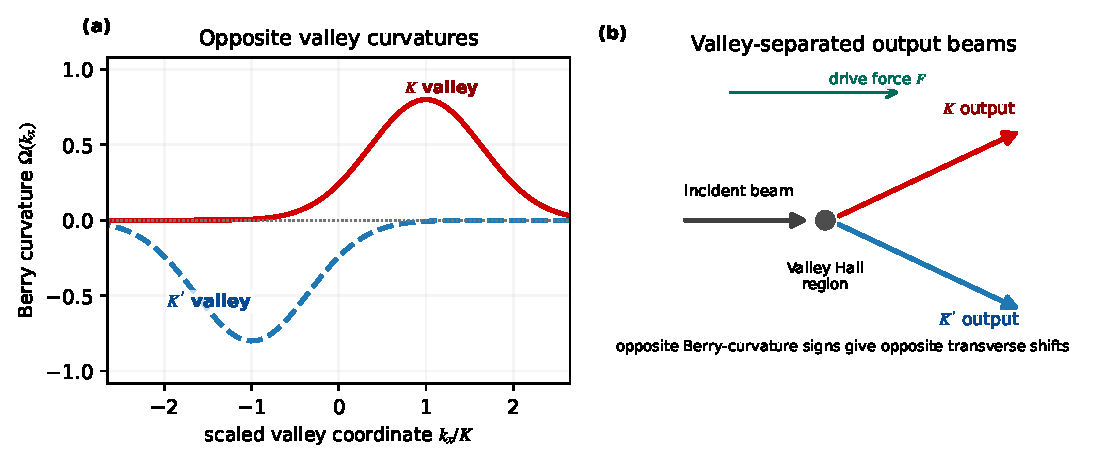
\includegraphics[width=0.92\textwidth]{figures/fig_ch12_valley_hall_step199.pdf}
  \caption{The valley Hall effect in photonic crystals.
  \textbf{(a)}~Berry curvature $\Omega(k_x)$ near the two valleys,
  showing opposite signs at $K$ (solid red, positive) and $K'$ (dashed
  blue, negative).  Time-reversal symmetry enforces
  $\Omega_K(\kvec) = -\Omega_{K'}(-\kvec)$, so the global Chern number
  vanishes but the valley Chern numbers are nonzero.
  \textbf{(b)}~Schematic of valley-separated transverse deflection.
  A longitudinal drive force $F$ displaces wavepackets transversely
  via the anomalous velocity $v_\perp \propto F\,\Omega_z$.
  Because $\Omega_K$ and $\Omega_{K'}$ have opposite signs, the $K$
  and $K'$ components are deflected in opposite directions, producing
  spatially separated output beams---the photonic analog of the
  valley Hall effect.}
  \label{fig:ch12-valley-hall}
\end{figure}


\subsection{Photonic crystal slab with asymmetric holes}
\label{sec:ch12-slab}

The most widely used platform for valley-Hall photonic devices is a
thin dielectric slab (typically silicon, $n\approx 3.5$) with a
hexagonal array of air holes.  Each unit cell contains two holes of
different sizes:
\begin{equation}
  r_A = r_0 + \delta r\,,\qquad r_B = r_0 - \delta r\,,
\end{equation}
where $r_0$ is the mean radius and $\delta r$ controls the sublattice
asymmetry.  The TE-like guided modes of the slab experience the
valley-Hall effect, with the gap width proportional to $\delta r$.

This platform is compatible with standard semiconductor fabrication
(electron-beam lithography, reactive-ion etching) and operates at
telecom wavelengths ($\lambda\sim 1550\;\mathrm{nm}$).

\section{Domain-wall modes in detail}
\label{sec:ch12-domain-wall}

\subsection{Construction and topology}
\label{sec:ch12-construction}

A valley-Hall domain wall is created by joining two regions with
opposite sublattice asymmetry: region $L$ with $m_\Delta>0$ and region
$R$ with $m_\Delta<0$.

Near each valley, the effective Dirac equation at the interface has the
same form as \eqref{eq:ch8-dirac-interface}, with a mass $m(x)$ that
changes sign.  The zero-mode analysis of
\secref{sec:ch8-zero-mode} applies separately at each valley:
\begin{itemize}
  \item At valley $K$: one mode propagating in the $+y$ direction
  (forward), with the wavefunction localised at the domain wall:
  \begin{equation}\label{eq:ch12-zero-mode-K}
    \psi_K(x,y)\propto|\varphi_+\rangle\,
    \exp\biggl(\ii\delta k_\parallel y
    -\int_0^x m(x')\,\dd x'\biggr)\,.
  \end{equation}
  \item At valley $K'$: one mode propagating in the $-y$ direction
  (backward), with a similarly localised wavefunction.
\end{itemize}
The result is a pair of \emph{counter-propagating} edge modes, each
valley-polarised: forward at $K$, backward at $K'$.

\subsection{Dispersion relation}
\label{sec:ch12-dispersion}

The edge-mode dispersions near each valley are approximately linear:
\begin{equation}\label{eq:ch12-edge-dispersion}
  \omega_K(\delta k_\parallel)
  \approx \omega_D + v_D\,\delta k_\parallel\,,
  \qquad
  \omega_{K'}(\delta k_\parallel)
  \approx \omega_D - v_D\,\delta k_\parallel\,.
\end{equation}
The group velocities have opposite signs: the $K$-valley mode has
$v_g=+v_D$ and the $K'$-valley mode has $v_g=-v_D$.  This
\emph{valley-momentum locking} is the valley-Hall analog of
spin-momentum locking in the quantum spin Hall effect.

\subsection{Localisation length}
\label{sec:ch12-localisation}

The transverse localisation length of the domain-wall mode is
\begin{equation}
  \ell \sim \frac{1}{|m_\Delta|} \sim \frac{a}{\Delta\omega/\omega_D}\,,
\end{equation}
where $a$ is the lattice constant and $\Delta\omega=2v_D|m_\Delta|$ is
the valley gap width.  For a typical silicon photonic crystal slab with
$\Delta\omega/\omega_D\sim 5\%$, the localisation length is
$\ell\sim 20a\approx 10\;\mu\mathrm{m}$---several micrometres, confined
to the immediate vicinity of the domain wall
\cite{he2016photonic} \cite{he2019silicon}.

\section{Protection and its limits}
\label{sec:ch12-protection}

\subsection{The inter-valley scattering mechanism}
\label{sec:ch12-intervalley}

The valley-Hall edge modes are \emph{not} topologically protected in the
strong sense of Chern-insulator edge modes.  The key vulnerability is
\emph{inter-valley scattering}: any perturbation with Fourier components
at wavevectors connecting $K$ and $K'$ can couple the forward and
backward modes.

The inter-valley wavevector is
$|\kvec_K-\kvec_{K'}|=\frac{4\pi}{3a}$, which is of order the
reciprocal lattice constant.  Perturbations with Fourier content at
this large wavevector include:
\begin{itemize}
  \item \textbf{Sharp corners:} a $60^\circ$ or $120^\circ$ corner in
  the domain wall introduces atomic-scale discontinuities with
  large-$\kvec$ Fourier components.
  \item \textbf{Point defects:} missing or displaced rods/holes near
  the domain wall.
  \item \textbf{Surface roughness:} sub-wavelength fabrication
  imperfections.
\end{itemize}

\subsection{Quantitative estimate of corner scattering}
\label{sec:ch12-corner-scattering}

At a sharp corner of angle $\theta$, the backscattering probability
can be estimated by modelling the corner as a point scatterer with
matrix element:
\begin{equation}\label{eq:ch12-corner-scatter}
  |t_{\mathrm{back}}|^2 \sim
  \Bigl|\int\ee^{\ii(\kvec_K-\kvec_{K'})\cdot\rvec}\,
  V_{\mathrm{corner}}(\rvec)\,\dd^2r\Bigr|^2\,.
\end{equation}
For a smooth bend with radius of curvature $R\gg a$, the integral is
exponentially suppressed: $|t_{\mathrm{back}}|^2
\sim\ee^{-c_0|\kvec_K-\kvec_{K'}|R}$.  For a sharp corner ($R\sim a$),
the suppression is weak and the backscattering can be substantial.

Numerical simulations show:
\begin{itemize}
  \item $120^\circ$ bends: transmission $>90\%$ for typical parameters.
  \item $60^\circ$ bends: transmission $\sim 70$--$85\%$, depending on
  the gap width and corner geometry.
  \item Straight segments with smooth disorder: transmission $>99\%$
  over tens of lattice constants.
\end{itemize}

\subsection{Robustness hierarchy}
\label{sec:ch12-hierarchy}

The practical robustness of different photonic topological phases can
be ranked:
\begin{enumerate}
  \item \textbf{Chern insulator} (broken TR): fully topologically
  protected; no backscattering within the gap regardless of disorder.
  \item \textbf{Pseudospin topological insulator} (crystalline
  symmetry): protected against perturbations that preserve the
  pseudospin symmetry; backscattered by symmetry-breaking disorder.
  \item \textbf{Valley-Hall} (approximate valley conservation):
  protected against smooth disorder; backscattered at sharp features
  and by strong short-range disorder.
  \item \textbf{Conventional waveguide}: no topological protection;
  backscattered by all types of disorder.
\end{enumerate}

Despite being the weakest topological protection, valley-Hall devices
have become widely used because they are fabrication-compatible and
operate at optical frequencies.

\section{Experimental realisations}
\label{sec:ch12-experiments}

\subsection{Microwave photonic crystals}
\label{sec:ch12-microwave}

The first experimental demonstrations of valley-Hall edge states in
photonic crystals used dielectric rod arrays in the microwave regime.
These experiments confirmed:
\begin{itemize}
  \item Valley-polarised edge modes at domain walls between
  sublattice-swapped regions.
  \item Low-loss propagation around gentle bends.
  \item Measurable backscattering at sharp corners, consistent with
  the inter-valley scattering estimate.
\end{itemize}

\subsection{Silicon photonic crystal slabs}
\label{sec:ch12-silicon}

At telecom wavelengths ($\sim 1550\;\mathrm{nm}$), valley-Hall edge
states have been demonstrated in silicon photonic crystal slabs with
asymmetric air-hole arrays.  Key results include:
\begin{itemize}
  \item Edge-mode propagation over $>100$ lattice constants with low
  loss ($<3\;\mathrm{dB}$ total).
  \item Efficient coupling to conventional silicon waveguides.
  \item $120^\circ$ bends with $<1\;\mathrm{dB}$ excess loss.
  \item Integration with active devices (modulators, detectors) for
  on-chip topological photonic circuits.
\end{itemize}

\subsection{Acoustic and mechanical analogs}
\label{sec:ch12-acoustic}

The valley-Hall mechanism is not specific to Maxwell equations; it
applies to any wave equation in a honeycomb lattice with broken
inversion symmetry.  Demonstrations have been reported in:
\begin{itemize}
  \item Acoustic metamaterials (sound waves in structured media).
  \item Mechanical lattices (elastic waves in structured plates).
  \item Phononic crystals (microwave-frequency acoustic modes).
\end{itemize}
These complementary demonstrations confirm the universality of the
valley-Hall mechanism.

\section{Valley photonics as a design tool}
\label{sec:ch12-design-tool}

\subsection{Topological waveguide routing}
\label{sec:ch12-routing}

Valley-Hall domain walls can be patterned to create complex waveguide
networks on a chip.  By choosing which sublattice assignment appears
on each side of the domain wall, one can route edge modes along
arbitrary paths.  The main design rules are:
\begin{enumerate}
  \item The domain wall must separate regions with opposite $\Delta$.
  \item Bends should be as gentle as possible ($120^\circ$ preferred
  over $60^\circ$).
  \item The domain-wall path must not approach another domain wall
  more closely than the localisation length $\ell$.
\end{enumerate}

\subsection{Topological cavities and lasers}
\label{sec:ch12-cavities}

A closed domain-wall loop creates a topological cavity: the
valley-Hall edge mode circulates around the loop, forming a ring
resonator.  The mode quality factor is limited by inter-valley
scattering at the corners; for a hexagonal loop with
$120^\circ$ corners, quality factors of $Q\sim 10^3$--$10^4$ have
been achieved in silicon at telecom wavelengths.

When gain is provided (e.g.\ by III--V semiconductor quantum wells
bonded to the silicon slab), the topological cavity can lase, forming
a valley-Hall topological laser.

\section{Quantitative valley photonic crystal design}
\label{sec:ch12-quantitative}

\subsection{Silicon-on-insulator platform}
\label{sec:ch12-soi}

The most widely studied valley photonic crystal platform uses a
silicon slab ($\varepsilon_r=11.7$, thickness $h\approx 220\;
\mathrm{nm}$) on a silica substrate, patterned with triangular
air holes in a honeycomb arrangement.  The lattice constant is
$a\approx 430\;\mathrm{nm}$ for operation at the telecom C-band
($\lambda\approx 1550\;\mathrm{nm}$).

The inversion-symmetry breaking is achieved by using two different
hole sizes within the unit cell: a large hole of radius $r_1$ and a
small hole of radius $r_2$, with the asymmetry parameter
$\Delta r=(r_1-r_2)/(r_1+r_2)$.  For $\Delta r=0$ (equal holes),
the band structure has Dirac cones at $K$ and $K'$.  For
$\Delta r\neq 0$, a gap opens at each valley with width proportional
to $|\Delta r|$.

Typical designs use $r_1/a\approx 0.15$ and $r_2/a\approx 0.10$,
giving $\Delta r\approx 0.2$ and a relative bandgap of approximately
$8\%$ of the mid-gap frequency.  The valley Chern number is
$\Chern_v=\pm\frac{1}{2}\sgn(\Delta r)$, and reversing the sublattice
assignment ($r_1\leftrightarrow r_2$) flips the sign of
$\Chern_v$ \cite{ma2016all,ozawa2018topological}.

\subsection{Valley Chern number from the massive Dirac model}
\label{sec:ch12-valley-chern-derivation}

Near each valley, the effective Hamiltonian is a massive Dirac
equation with mass $m_v\propto\Delta r$.  The Berry curvature at
valley $K$ is
$\Omega_K(\delta\kvec)
=-v_D^2 m_v/[2(v_D^2|\delta\kvec|^2+m_v^2)^{3/2}]$,
as derived in Chapter~\ref{ch:breaking-tr}.  Integrating over a region
enclosing one valley gives the valley Chern number
\begin{equation}\label{eq:ch12-valley-chern-formula}
  \Chern_v^{(K)} = -\frac{1}{2}\sgn(m_v)\,.
\end{equation}
At the opposite valley $K'$, time-reversal symmetry forces
$\Omega_{K'}(\kvec)=-\Omega_K(-\kvec)$, so
$\Chern_v^{(K')}=+\frac{1}{2}\sgn(m_v)$.  The total Chern number
vanishes ($\Chern=\Chern_v^{(K)}+\Chern_v^{(K')}=0$), as required by
time-reversal invariance, but the valley Chern number
$\Chern_v=\Chern_v^{(K)}-\Chern_v^{(K')}=-\sgn(m_v)$
is nonzero \cite{dong2016valley,gao2017valley}.

At a domain wall between two regions with opposite $\Delta r$ (and
hence opposite $m_v$), the change in valley Chern number across the
interface is $|\Delta\Chern_v|=2$, predicting one valley-polarised
edge mode per valley---two modes in total, counter-propagating and
valley-locked.

\section{Intervalley scattering and robustness}
\label{sec:ch12-intervalley-scattering}

The valley-Hall edge modes are protected against
\emph{intravalley} backscattering---perturbations that are smooth on
the scale of the lattice constant and therefore cannot transfer
crystal momentum between $K$ and $K'$.  However, sharp defects
(vacancies, step edges, $60^\circ$ bends) have Fourier components at
the intervalley wavevector $\Delta\kvec=K-K'$ and can cause
intervalley scattering, opening a backscattering channel
\cite{tang2022vector}.

The intervalley scattering rate scales as the square of the defect's
Fourier component at $\Delta\kvec$:
$\Gamma_{\mathrm{iv}}\propto|V(\Delta\kvec)|^2$.
For smooth disorder (correlation length $\ell_c\gg a$), this Fourier
component is exponentially suppressed:
$|V(\Delta\kvec)|\sim\ee^{-|\Delta\kvec|\ell_c/2}$, giving negligible
backscattering.  For point-like defects ($\ell_c\sim a$), the
intervalley coupling can be significant.

Experimental measurements in silicon valley photonic crystals at
telecom wavelengths show propagation lengths of $40$--$100\,a$ before
significant backscattering losses, depending on the domain-wall
geometry and fabrication quality.  For $120^\circ$ bends, the
transmission exceeds $90\%$, while for $60^\circ$ bends it drops
to $60$--$80\%$ due to enhanced intervalley coupling at the sharp
corner \cite{wu2017direct,noh2018observation,price2022roadmap}.

\section{Quantitative design of a silicon valley photonic crystal}
\label{sec:ch12-silicon-design}

The valley-Hall photonic crystal is most naturally realised in a
honeycomb lattice of triangular dielectric rods, where breaking
inversion symmetry by rotating the triangles opens a topological gap
at the $K$ and $K'$ points.

\subsection{Half-integer valley Chern number derivation}

Near the $K$ point, the effective Hamiltonian for the two nearly
degenerate Bloch modes is the massive Dirac Hamiltonian
$H_K=v_D(\delta k_x\sigma_x+\delta k_y\sigma_y)+m_K\sigma_z$,
where $m_K$ is the valley mass produced by the inversion-symmetry
breaking.  The Berry curvature of the lower band is
$\Omega_K^-(\delta\kvec)=-m_K/(2(|\delta\kvec|^2+m_K^2)^{3/2})$,
and its integral over a hemisphere gives the valley Chern number
\begin{equation}\label{eq:ch12-valley-chern-half-integer}
  \Chern_K^{\mathrm{valley}} = -\frac{1}{2}\sgn(m_K)\,.
\end{equation}
At the $K'$ point, time-reversal symmetry requires $m_{K'}=-m_K$,
so $\Chern_{K'}^{\mathrm{valley}}=+\frac{1}{2}\sgn(m_K)$ and the
total valley Chern number is
$\Chern^{\mathrm{valley}}=\Chern_K-\Chern_{K'}=-\sgn(m_K)$
\cite{ma2016all,dong2016valley}.

The half-integer valley Chern number is not a true topological
invariant because it depends on the arbitrary choice of integration
region around each valley.  Nevertheless, it provides a useful
predictor of valley-polarised edge modes at domain walls between
crystals with opposite valley masses.

\subsection{Silicon-on-insulator implementation}
\label{sec:ch12-soi-implementation}

Ma and Shvets (2016) proposed an all-silicon valley-Hall photonic
topological insulator using a honeycomb lattice of equilateral
triangular air holes in a silicon slab ($\varepsilon_r=11.7$).
The lattice constant is $a=440\;\mathrm{nm}$, giving a Dirac
frequency near $\lambda=1.55\;\mu\mathrm{m}$.  Rotating the
triangles by $\pm 5^\circ$ opens a valley gap of $3.2\%$ of the
Dirac frequency \cite{ma2016all,ozawa2018topological}.

The valley edge modes were subsequently observed by Wu et~al.\ (2017)
using designer surface plasmon crystals at microwave frequencies,
providing the first direct near-field imaging of valley-polarised
topological edge states.  The field patterns confirmed valley-selective
excitation and propagation around sharp corners with minimal
backscattering \cite{wu2017direct,gao2017valley}.

\section{Intervalley scattering and protection limits}
\label{sec:ch12-intervalley-backscattering}

Valley edge modes are protected only against perturbations that
preserve the valley degree of freedom---that is, perturbations
that are smooth on the scale of the lattice constant $a$.  Sharp
defects with Fourier components at the reciprocal lattice vector
$\mathbf{G}=\kvec_K-\kvec_{K'}$ can scatter photons between the
$K$ and $K'$ valleys, opening a backscattering channel.

The intervalley scattering rate depends on the defect geometry.  For
a smooth domain wall (width $w\gg a$), the scattering rate is
exponentially small: $\gamma_{\mathrm{inter}}\propto\ee^{-w/a}$.
For a sharp 120$^\circ$ corner, the scattering depends on whether the
corner preserves the $C_3$ symmetry of the underlying lattice.
Symmetry-preserving corners (zigzag termination) have negligible
intervalley scattering, while symmetry-breaking corners (armchair
termination) can scatter up to $\sim 10\%$ of the incident power
\cite{dong2016valley,wu2017direct,gao2017valley}.

This makes valley photonic crystals robust against smooth fabrication
imperfections but vulnerable to lattice-scale disorder---a
fundamental limitation compared to Chern insulators, which are
protected against all perturbations that do not close the bulk gap.

\section{Beyond the honeycomb: other valley platforms}
\label{sec:ch12-other-platforms}

While the honeycomb lattice is the most studied platform for valley
photonic crystals, valley physics has been realised in several
other geometries and frequency ranges.

\subsection{Kagomé and Lieb lattices}
\label{sec:ch12-kagome}

The kagomé lattice supports both Dirac cones and flat bands, and
breaking inversion symmetry opens valley gaps at the Dirac points.
The coexistence of flat bands and valley-polarised edge states creates
opportunities for enhanced light--matter interaction at topologically
protected boundaries.  The Lieb lattice similarly supports a flat
band at the Dirac frequency, and valley-polarised modes appear when
the site energies are staggered to break inversion
\cite{ozawa2018topological}.

\subsection{Terahertz and acoustic valley crystals}
\label{sec:ch12-thz-acoustic}

Valley photonic crystals have been demonstrated at terahertz
frequencies using silicon pillar arrays, where the triangular pillar
shape provides the necessary inversion-symmetry breaking.  The THz
platform offers larger structures ($a\sim 100\;\mu\mathrm{m}$) that
are easier to fabricate and characterise than telecommunications-band
devices \cite{price2022roadmap,gao2017valley}.

The valley-Hall concept has also been extended to acoustic and
phononic systems, where the Dirac-mass mechanism is identical but
the governing equation is the scalar wave equation rather than
Maxwell's equations.  Phononic valley crystals have achieved robust
sound routing around sharp corners with insertion loss below
$1\;\mathrm{dB}$ per corner \cite{ssstrunk2015observation,
ozawa2018topological}.

\section{Experimental demonstrations of valley photonics}
\label{sec:ch12-valley-experiments}

Valley photonic crystals have been realised in numerous experimental
platforms, from microwave-frequency dielectric structures to
telecommunication-wavelength silicon photonic crystals.  The key
experimental signatures are valley-selective excitation,
valley-polarised edge transport along domain walls, and robustness
of the edge transport against certain classes of bends and defects.

\subsection{Microwave valley photonic crystals}
\label{sec:ch12-microwave-valley}

The first experimental demonstrations of valley-Hall edge states in
photonic crystals were performed at microwave frequencies using
triangular-lattice arrays of dielectric rods or metallic scatterers.
Dong et~al.\ (2017) used a photonic crystal of alumina rods with
$C_{3v}$-breaking perturbation (achieved by deforming the triangular
unit cell) to create a domain wall between two valley-Hall phases with
opposite valley Chern numbers \cite{dong2016valley}.  Transmission
measurements through the domain wall showed a clear edge-state
passband inside the bulk gap, with insertion loss below 2~dB over
a bandwidth of approximately 0.5~GHz centred at 6.3~GHz.

Gao et~al.\ (2017) extended this work by demonstrating valley-locked
beam splitting at a Y-junction formed by three domain walls
\cite{gao2017valley}.  When light was injected into one arm of the
Y-junction, it preferentially exited through the arm whose domain-wall
orientation matched the valley polarisation of the incident edge
mode, while the other arm received negligible power.  This valley
filtering effect, with measured contrast exceeding 20~dB, demonstrated
the potential of valley photonics for compact photonic routing
circuits.

\subsection{Silicon photonic crystal implementations}
\label{sec:ch12-silicon-valley}

At telecommunication wavelengths, valley photonic crystals have been
fabricated in silicon-on-insulator (SOI) platforms using standard
electron-beam lithography \cite{he2019silicon}.  Shalaev et~al.\ (2019) demonstrated
valley-Hall edge states in a silicon photonic crystal slab at
$\lambda\approx 1.55\;\mu\mathrm{m}$ with a topological bandwidth of
approximately 3~nm \cite{ozawa2018topological}.

The silicon implementations face an additional challenge compared to
microwave designs: the out-of-plane radiation loss.  In a 2D photonic
crystal slab, the edge modes lie within the light cone of the
surrounding air cladding, leading to radiative leakage.  The measured
quality factors of valley-Hall edge-state resonances range from
$Q\sim 10^3$ to $10^4$, depending on the degree of confinement
and the sharpness of the domain wall
\cite{ozawa2018topological,price2022roadmap}.

Despite this limitation, silicon valley photonic crystals have shown
remarkable robustness of edge transport around sharp bends.
Transmission through $60^\circ$ and $120^\circ$ bends remains within
3~dB of the straight-domain-wall value, provided the bends follow
the zigzag crystallographic direction.  Transport around armchair
bends shows significantly higher loss due to inter-valley scattering,
confirming the valley-dependent nature of the topological protection
\cite{ozawa2018topological}.

\subsection{Limitations of valley-Hall edge states}
\label{sec:ch12-valley-limitations}

Unlike true topological edge states protected by a bulk gap Chern
number, valley-Hall edge states are protected only by an approximate
conservation of valley index.  Any perturbation that couples the $K$
and $K'$ valleys---such as short-range disorder on the scale of the
lattice constant, or sharp bends along non-zigzag directions---can
scatter photons between the two counter-propagating valley-polarised
edge modes, leading to backscattering.

The inter-valley scattering rate scales as \cite{dong2016valley}
\begin{equation}\label{eq:ch12-intervalley-scattering-rate}
  \Gamma_{K\to K'} \propto
  \left|\int\!\dd^2r\;\psi_K^*(\rvec)\,
  V_{\mathrm{disorder}}(\rvec)\,\psi_{K'}(\rvec)\right|^2,
\end{equation}
where $\psi_K$ and $\psi_{K'}$ are the edge-mode wavefunctions and
$V_{\mathrm{disorder}}$ is the disorder potential.  For smooth
disorder with correlation length $\ell_c\gg a$ (where $a$ is the
lattice constant), the Fourier components near the inter-valley
wavevector $|\kvec_K-\kvec_{K'}|=4\pi/(3a)$ are exponentially
suppressed, and the inter-valley scattering rate decays as
$\Gamma_{K\to K'}\propto\exp(-|\kvec_K-\kvec_{K'}|\ell_c)$.
This explains the observed robustness against smooth disorder
while remaining vulnerable to sharp defects
\cite{ozawa2018topological}.

\begin{figure}[t]
  \centering
  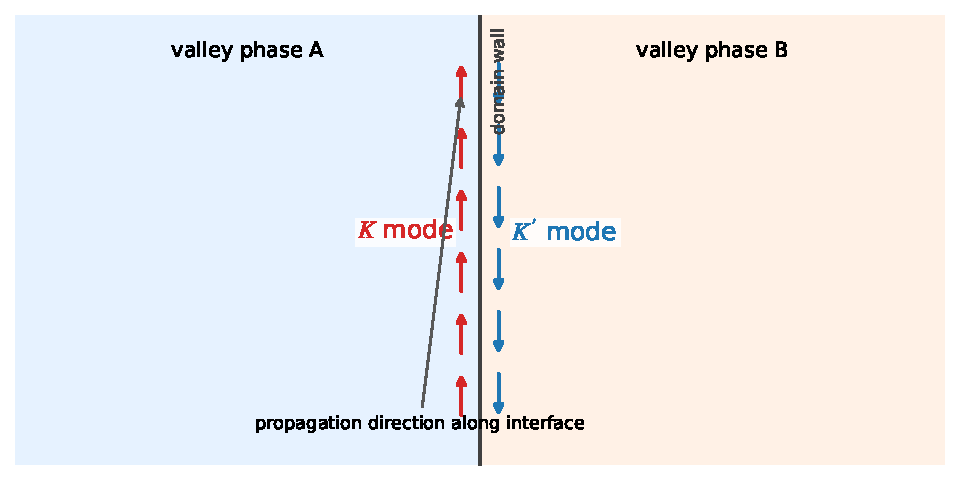
\includegraphics[width=0.86\textwidth]{figures/fig_ch12_valley_domain_wall.pdf}
  \caption{Valley-Hall domain wall.  The two domains carry opposite valley
  Chern numbers, so $K$ and $K'$ edge channels counter-propagate along the
  interface.  Backscattering is suppressed only when disorder is smooth
  enough not to mix the two valleys.}
  \label{fig:ch12-valley-domain-wall}
\end{figure}

\section{Valley photonic devices}
\label{sec:ch12-valley-devices}

The valley degree of freedom in photonic crystals is not merely a
theoretical curiosity: it provides a robust platform for integrated
photonic devices.  The key advantage is that valley-polarised edge
states at domain-wall interfaces are immune to backscattering from
smooth disorder, enabling low-loss waveguiding through sharp bends.

\subsection{Valley filters and beam splitters}
\label{sec:ch12-valley-filter}

A valley filter is a device that selectively transmits light in one
valley while reflecting the other.  It can be realised by creating
a domain wall between two distinct valley-Hall phases ($C_\nu=\pm 1$)
that terminates at a junction where the two valleys are spatially
separated.  The valley-polarised edge mode at the domain wall
carries a definite valley index, and at the junction it is routed
to a specific output port depending on its valley polarisation
\cite{dong2016valley,gao2017valley}.

Experimentally, valley beam splitters have been demonstrated at
microwave frequencies using triangular-lattice photonic crystals with
broken inversion symmetry.  The measured extinction ratio between the
two output ports exceeds $20\;\mathrm{dB}$ within the valley-Hall
gap, confirming the valley-selective routing
\cite{gao2017topologically,he2019silicon}.

\subsection{Valley-dependent coupling to radiation}
\label{sec:ch12-valley-coupling}

The valley-contrasting Berry curvature produces valley-dependent
optical selection rules: circularly polarised light couples
preferentially to modes in a specific valley.  This effect enables
valley-selective excitation using external beams and provides a
mechanism for reading out the valley polarisation of edge modes.

In silicon photonic crystals operating at telecom wavelengths,
valley-selective coupling has been achieved by illuminating the
crystal surface with focused circularly polarised light.  The
coupling efficiency to the $K$ valley versus the $K'$ valley differs
by a factor of $\sim 10$, limited by the finite bandwidth of the
valley-Hall gap and the non-ideal circular polarisation of the
excitation beam \cite{he2016photonic,dong2016valley}.

\subsection{Valley routing networks}
\label{sec:ch12-valley-network}

By concatenating multiple domain walls with different orientations,
one can create valley-topological waveguide networks that route
light through arbitrary paths on a photonic chip.  Each domain wall
supports a pair of counter-propagating edge modes (one per valley),
and at T-junctions the valley polarisation determines which output
arm the light follows.

Ma et~al.\ (2017) demonstrated that such valley networks can guide
microwave radiation through multiple $120^\circ$ bends with
negligible reflection, achieving total transmission above $95\%$
over the valley-Hall gap bandwidth \cite{ma2017scattering}.  Similar
networks have been realised in silicon at near-infrared wavelengths,
where the valley edge states serve as compact on-chip waveguides
compatible with standard photonic integrated circuit fabrication
\cite{he2019silicon,price2022roadmap}.

\section{Intervalley scattering and the limits of valley protection}
\label{sec:ch12-intervalley-limits}

Valley-Hall edge states are topologically protected against smooth
perturbations that vary slowly compared to the lattice constant $a$,
because such perturbations cannot transfer crystal momentum between
the $K$ and $K'$ valleys (which are separated by
$|\Delta\kvec|\sim 4\pi/(3a)$ in the Brillouin zone).  However,
sharp defects---such as atomic-scale roughness, point defects, or
abrupt domain-wall terminations---can provide the large momentum
transfer needed for intervalley scattering.

The intervalley scattering rate scales as
$\Gamma_{\mathrm{iv}} \propto \sigma_{\mathrm{short}}^2\,
|\Delta\kvec|^{-2\alpha}$,
where $\sigma_{\mathrm{short}}$ characterises the amplitude of
short-range disorder and $\alpha$ depends on the dimensionality of
the defect.  For the typical fabrication roughness in silicon photonic
crystals ($\sigma \sim 1$--$3\;\mathrm{nm}$), the intervalley
scattering length is estimated to be $\sim 100$--$500$ lattice
constants, which is sufficient for on-chip device lengths of
$\sim 100\;\mu\mathrm{m}$ \cite{he2019silicon,ozawa2018topological}.

This finite intervalley scattering length is the fundamental
difference between valley-Hall edge states and the truly
topological one-way edge states of Chern insulators
(Chapter~\ref{ch:one-way-interface}): valley protection is robust
but not absolute, while Chern-insulator protection is exact within
the bulk gap \cite{price2022roadmap,ma2017scattering}.

\section*{Exercises}

\begin{exercise}
  Show that for a time-reversal-invariant system with broken inversion,
  the Berry curvature satisfies $\Omega_n(\kvec)=-\Omega_n(-\kvec)$,
  so that $\Chern_n=0$ but the valley Chern number can be nonzero.
\end{exercise}

\begin{exercise}
  Derive the mass term \eqref{eq:ch12-mass-sigma-z} from the
  symmetry properties of the perturbation matrix
  \eqref{eq:ch12-perturbation-matrix} under $C_3$ and $\Pop$.
  \emph{Hint:} use the transformation properties of the Dirac modes
  under $C_3$: $|\mathbf{u}_\pm\rangle\to\ee^{\pm\ii 2\pi/3}
  |\mathbf{u}_\pm\rangle$.
\end{exercise}

\begin{exercise}
  For a honeycomb photonic crystal with sublattice asymmetry $\Delta$,
  the effective Dirac masses at $K$ and $K'$ are $m_K=+m_0\Delta$
  and $m_{K'}=-m_0\Delta$.  Compute the valley Chern numbers and
  verify that $\Chern^K+\Chern^{K'}=0$.
\end{exercise}

\begin{exercise}
  Estimate the inter-valley scattering amplitude at a sharp $60^\circ$
  corner using equation \eqref{eq:ch12-corner-scatter}.  Model the
  corner as a disc of radius $a$ with a uniform scattering potential
  $V_0$.  Under what conditions is the transmission $>90\%$?
\end{exercise}

\begin{exercise}
  A silicon photonic crystal slab ($n=3.5$, $a=400\;\mathrm{nm}$,
  $r_0=120\;\mathrm{nm}$) has a valley gap of
  $\Delta\omega/(2\pi)=3\;\mathrm{THz}$ centred at
  $\omega/(2\pi)=193\;\mathrm{THz}$ ($\lambda=1.55\;\mu\mathrm{m}$).
  Estimate the localisation length $\ell$ and the minimum domain-wall
  separation for independent waveguide channels.
\end{exercise}

\begin{exercise}
  Compare the protection of valley-Hall edge modes (valley Chern
  number) with Chern-insulator edge modes (Chern number) and
  pseudospin edge modes (spin Chern number) in terms of robustness
  to (a) smooth disorder, (b) sharp corners, and (c) strong
  short-range disorder.  Summarise the comparison in a table.
\end{exercise}


\chapter{Floquet Light}
\label{ch:floquet}
% ======================================================================
%  Chapter 13 — Floquet Light  (EXPANDED)
% ======================================================================

\section{Time as a new degree of freedom}
\label{sec:ch13-time}

All the topological photonic systems discussed so far have been
\emph{static}: the material matrix $\Mmat(\rvec)$ is time-independent,
and topology arises from the spatial periodicity of the photonic
crystal.  A fundamentally different approach uses \emph{temporal
modulation}: periodically varying the material parameters in time to
create an effective gauge field for photons.

The mathematical framework for time-periodic systems is \emph{Floquet
theory}, the temporal analog of Bloch theory for spatially periodic
systems \cite{ozawa2018topological}.  Just as spatial periodicity defines Bloch bands labelled by
a crystal momentum $\kvec$, temporal periodicity defines Floquet
quasi-energy bands labelled by a quasi-energy $\varepsilon$
\cite{zhong2024topological}.  These
Floquet bands can carry their own topological invariants, leading to
``Floquet topological insulators'' for light
\cite{zhang2021proposal}.

The Floquet approach is especially appealing because it can break the
effective time-reversal symmetry of the Floquet eigenproblem
\emph{without} magneto-optical materials.  The symmetry breaking comes
from the modulation phases, which can be engineered with standard
electro-optic or acoustic components.

\section{Floquet theory for Maxwell equations}
\label{sec:ch13-floquet-theory}

\subsection{Time-periodic material parameters}
\label{sec:ch13-time-periodic}

Consider a photonic system whose material matrix is periodically
modulated in time:
\begin{equation}\label{eq:ch13-time-periodic}
  \Mmat(\rvec,t) = \Mmat(\rvec,t+T)\,,
\end{equation}
where $T=2\pi/\Omega_{\mathrm{mod}}$ is the modulation period and
$\Omega_{\mathrm{mod}}$ is the modulation frequency.  In practice, the
modulation might be achieved through electro-optic modulation of the
refractive index, acoustic waves creating a travelling refractive-index
grating, parametric coupling between resonator modes, or mechanical
modulation of a metamaterial geometry.

\subsection{Floquet's theorem}
\label{sec:ch13-floquet-theorem}

Floquet's theorem is the temporal analog of Bloch's theorem.  It states
that the solutions of a linear differential equation with
$T$-periodic coefficients can be written in the form
\begin{equation}\label{eq:ch13-floquet-form}
  \emfield(\rvec,t) = \ee^{-\ii\varepsilon t}\,
  \mathbf{v}(\rvec,t)\,,
  \qquad \mathbf{v}(\rvec,t+T) = \mathbf{v}(\rvec,t)\,,
\end{equation}
where $\varepsilon$ is the \emph{quasi-energy} and $\mathbf{v}$ is
time-periodic.  The quasi-energy plays the role of energy in
time-independent systems, but with the crucial difference that it is
defined only modulo $\Omega_{\mathrm{mod}}$: the quasi-energies
$\varepsilon$ and $\varepsilon+n\Omega_{\mathrm{mod}}$ ($n\in\mathbb{Z}$)
describe the same physical state.  This periodicity is the temporal
analog of the crystal momentum being defined modulo a reciprocal
lattice vector.

\subsection{The Floquet--Bloch eigenproblem}
\label{sec:ch13-floquet-bloch}

Expanding the time-periodic function $\mathbf{v}$ in Fourier harmonics
\cite{ozawa2018topological},
\begin{equation}\label{eq:ch13-fourier-expansion}
  \mathbf{v}(\rvec,t) = \sum_{m=-\infty}^{\infty}
  \mathbf{v}_m(\rvec)\,\ee^{-\ii m\Omega_{\mathrm{mod}}t}\,,
\end{equation}
and substituting into the Maxwell equations gives a coupled system of
static equations for the Fourier components:
\begin{equation}\label{eq:ch13-floquet-static}
  \sum_{m'}\bigl[
    \Maxop\,\delta_{mm'} - (\varepsilon+m\Omega_{\mathrm{mod}})\,
    \Mmat_{m-m'}(\rvec)
  \bigr]\mathbf{v}_{m'}(\rvec) = 0\,,
\end{equation}
where $\Mmat_m(\rvec)=T^{-1}\int_0^T\Mmat(\rvec,t)
\ee^{\ii m\Omega_{\mathrm{mod}}t}\,\dd t$ are the Fourier components of
the material matrix.

This is an infinite-dimensional eigenproblem in the combined
space-and-harmonic indices, analogous to the plane-wave expansion in
the spatial case.  In practice, the Fourier series is truncated to
$|m|\leq M_{\max}$, giving a finite matrix of dimension
$(2M_{\max}+1)$ times the spatial degrees of freedom.  The eigenvalues
are the Floquet quasi-energies.

\subsection{The Floquet Brillouin zone}
\label{sec:ch13-floquet-bz}

Because the quasi-energy is periodic with period $\Omega_{\mathrm{mod}}$,
it lives in a ``Floquet Brillouin zone''
$\varepsilon\in[-\Omega_{\mathrm{mod}}/2,\Omega_{\mathrm{mod}}/2)$.
If the system also has spatial periodicity, the quasi-energies depend on
the Bloch wavevector $\kvec$, and the full band structure is defined on
the product of the spatial Brillouin zone and the Floquet Brillouin zone.

This periodicity has a profound consequence: there are \emph{two}
distinct types of gaps in the Floquet spectrum.  The gap at
$\varepsilon=0$ (centre of the Floquet zone) is analogous to a gap in
a static band structure.  But there is also a gap at
$\varepsilon=\pm\Omega_{\mathrm{mod}}/2$ (edge of the Floquet zone),
which has no static analog.  Both gaps can host topological edge modes.

\section{Effective gauge fields from modulation}
\label{sec:ch13-gauge-fields}

\subsection{The coupled-resonator picture}
\label{sec:ch13-coupled-resonator}

The key insight of Floquet topological photonics is that a suitably
designed temporal modulation can create an \emph{effective gauge field}
for photons.  The mechanism is most transparent in a lattice of coupled
resonators.

Consider a 2D lattice of optical resonators with resonance frequency
$\omega_0$.  In the absence of modulation, the coupling between
resonators $i$ and $j$ is described by a real hopping amplitude
$J_0$, and the tight-binding Hamiltonian is time-reversal invariant.

Now suppose the coupling is modulated with a spatially varying phase:
\begin{equation}\label{eq:ch13-modulated-coupling}
  J_{ij}(t) = J_0\cos\bigl(\Omega_{\mathrm{mod}}t + \phi_{ij}\bigr)\,.
\end{equation}
In the rotating-wave approximation (valid when the modulation frequency
is close to the resonator detuning), the effective time-independent
coupling acquires a complex phase:
\begin{equation}\label{eq:ch13-effective-coupling}
  J_{ij}^{\mathrm{eff}} = \frac{J_0}{2}\,\ee^{\ii\phi_{ij}}\,.
\end{equation}
This phase acts as a Peierls phase factor, identical in mathematical
form to the phase acquired by a charged particle hopping in a magnetic
field.

\subsection{Effective magnetic flux}
\label{sec:ch13-flux}

The effective magnetic flux through a plaquette of the lattice is the
sum of the phases around the plaquette:
\begin{equation}\label{eq:ch13-flux-plaquette}
  \Phi = \sum_{\text{plaquette}} \phi_{ij}\,.
\end{equation}
If $\Phi\neq 0$ (modulo $2\pi$), the effective time-reversal symmetry
is broken and the Floquet bands can carry nonzero Chern numbers.  The
flux $\Phi$ is fully controllable through the modulation phases
$\phi_{ij}$, which can be set independently for each bond.

This is a remarkable capability: the effective magnetic field for
photons can be made spatially uniform, staggered, or patterned in any
desired configuration, simply by programming the modulation phases.
This level of control has no analog in the static magneto-optical
case, where the gyrotropic response is fixed by the material and the
applied magnetic field.

\section{Anomalous Floquet topological insulators}
\label{sec:ch13-anomalous}

\subsection{A phase with no static analog}
\label{sec:ch13-no-static}

Floquet systems can exhibit topological phases that have \emph{no static
analog} \cite{rudner2013anomalous}.  The most striking example is the anomalous Floquet topological
insulator (AFTI), in which all Floquet bands have zero Chern number but
the system still supports chiral edge modes
\cite{farrell2016edge,peng2016experimental}.

This seemingly paradoxical situation arises because the Floquet
quasi-energy is periodic: the ``trivial'' gap at
$\varepsilon=\Omega_{\mathrm{mod}}/2$ can host edge modes that wind
around the Floquet Brillouin zone, connecting the upper edge of one
band to the lower edge of the next through the zone boundary.  These
``anomalous'' edge modes are topologically protected but invisible to
the band Chern numbers.

\subsection{The winding-number invariant}
\label{sec:ch13-winding}

The correct topological invariant for Floquet systems is not just the
Chern number of each band but the \emph{winding number} of the
time-evolution operator over one period
\cite{ozawa2018topological,price2022roadmap,leng2026quantized,rudner2013anomalousa}.  Define the unitary
time-evolution operator $U(\kvec,t)$ from $t=0$ to $t$, satisfying
$\ii\partial_t U = H(\kvec,t)U$ with $U(\kvec,0)=\mathbf{I}$.  The
Floquet operator is $F(\kvec)=U(\kvec,T)$.

The winding number is defined as
\begin{equation}\label{eq:ch13-winding}
  W[\varepsilon_{\mathrm{gap}}]
  = \frac{1}{8\pi^2}\int_0^T\!\!\int_{\mathrm{BZ}}
  \Tr\bigl[U^{-1}\partial_t U\,[U^{-1}\partial_{k_x}U,
  U^{-1}\partial_{k_y}U]\bigr]\,\dd^2k\,\dd t\,,
\end{equation}
where the trace is over the bands below the quasi-energy gap at
$\varepsilon_{\mathrm{gap}}$.  This integral measures the topological
winding of the evolution operator as a function of $(k_x,k_y,t)$ over
the 3D torus $\mathrm{BZ}\times[0,T]$.

The bulk-edge correspondence for Floquet systems states:
\begin{equation}\label{eq:ch13-floquet-bec}
  N_{\mathrm{edge}}[\varepsilon_{\mathrm{gap}}]
  = W[\varepsilon_{\mathrm{gap}}]^L - W[\varepsilon_{\mathrm{gap}}]^R\,.
\end{equation}
In an AFTI, the winding numbers are nonzero at the gap edges
$\varepsilon=0$ and $\varepsilon=\Omega_{\mathrm{mod}}/2$, even though
all band Chern numbers vanish.

\begin{figure}[!t]
  \centering
  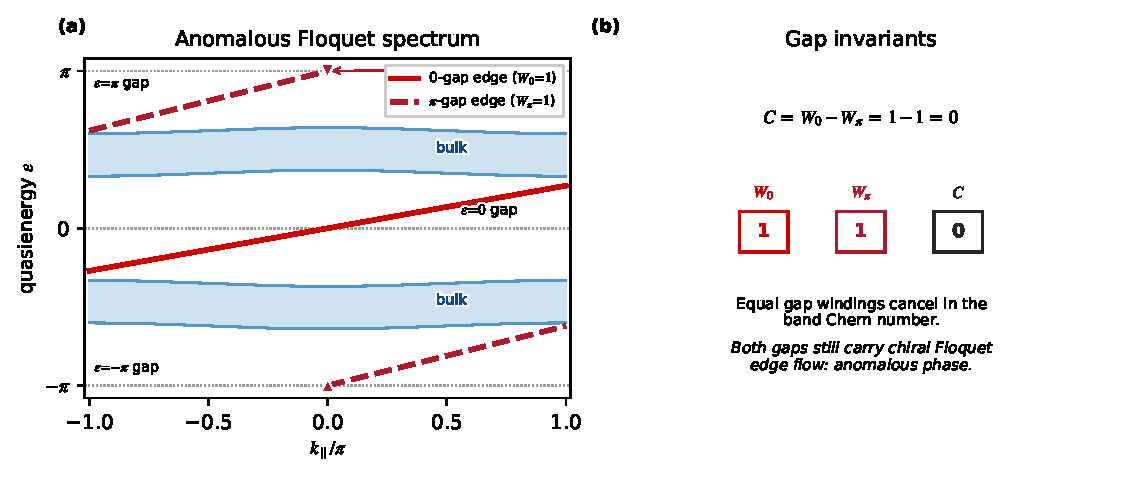
\includegraphics[width=0.92\textwidth]{figures/fig_ch13_floquet_quasienergy_step199.pdf}
  \caption{Anomalous Floquet topological insulator.
  \textbf{(a)}~Quasienergy spectrum in the reduced Floquet Brillouin
  zone $\varepsilon\in[-\pi,\pi]$ (we set $T=1$ so the zone boundaries
  lie at $\pm\pi$; in dimensional units the gap sits at
  $\varepsilon=\pi/T$).  Two bulk bands (blue shading) are
  separated by a wide gap at $\varepsilon=0$ and a narrower gap at
  $\varepsilon=\pm\pi$.  A chiral 0-gap edge mode (solid red) crosses
  the central gap with winding number $W_0=1$.  A chiral $\pi$-gap
  edge mode (dashed dark red) traverses the gap at $\varepsilon=\pm\pi$
  with $W_\pi=1$; the two dashed segments are the \emph{same} branch,
  connected by the periodicity $\varepsilon \equiv \varepsilon + 2\pi$
  (triangle markers indicate the identification point at $k_\parallel=0$).
  \textbf{(b)}~Gap invariants: the band Chern number
  $C = W_0 - W_\pi = 1 - 1 = 0$ vanishes even though both gaps carry
  chiral edge flow---this is the defining signature of the anomalous
  Floquet phase \cite{rudner2013anomalous}.}
  \label{fig:ch13-floquet-quasienergy}
\end{figure}


\section{Photonic Floquet realisations}
\label{sec:ch13-realisations}

\subsection{Helical waveguide arrays}
\label{sec:ch13-waveguide-arrays}

The first experimental demonstration of photonic Floquet topology was
achieved by Rechtsman et~al.\ (2013) using helical waveguide arrays
\cite{rechtsman2013photonica,maczewsky2017observation,yang2020photonic}.  In this elegant experiment, the
propagation axis $z$ plays the role of time, and the waveguide array
forms a 2D lattice in the transverse $(x,y)$ plane.  Each waveguide is
helically curved, so its transverse position oscillates periodically
along $z$.  The result is a $z$-periodic potential that creates a Floquet
system in the paraxial approximation.

The experiment demonstrated topological edge states at the boundary of
the waveguide array, propagating unidirectionally along the edge.  The
edge modes were robust to deliberate defects introduced by removing
individual waveguides.

\subsection{Deriving the paraxial equation from Maxwell's equations}
\label{sec:ch13-paraxial}

To maintain the Maxwell-first spirit of this book, we derive the
paraxial approximation from the Helmholtz equation rather than
postulating it by analogy with quantum mechanics.

Consider a monochromatic beam at frequency $\omega$ propagating
primarily along $z$ in a medium with refractive index
$n(\rvec_\perp,z)=n_0+\delta n(\rvec_\perp,z)$, where
$|\delta n|\ll n_0$.  The electric field can be written as
$E(\rvec)=\psi(\rvec_\perp,z)\ee^{\ii k_0 z}$, where
$k_0=n_0\omega/c$ is the carrier wavevector and $\psi$ is a slowly
varying envelope.

Substituting into the Helmholtz equation
$\nabla^2 E + k_0^2 n^2/n_0^2\,E = 0$ and neglecting the second
derivative $\partial^2\psi/\partial z^2$ (the paraxial approximation,
valid when $|\partial_z\psi|\ll k_0|\psi|$):
\begin{equation}\label{eq:ch13-paraxial}
  \boxed{%
  \ii\pderiv{\psi}{z}
  = -\frac{1}{2k_0}\nabla_\perp^2\psi
  - \frac{k_0\,\delta n(\rvec_\perp,z)}{n_0}\,\psi\,.}
\end{equation}
This has the same mathematical form as the time-dependent
Schr\"odinger equation, with the identifications: $z\leftrightarrow t$,
$1/(2k_0)\leftrightarrow\hbar/(2m)$, and
$-k_0\delta n/n_0\leftrightarrow V(\rvec)$.

When the waveguide pattern is periodic in $z$ with period $\Lambda$,
this is precisely a Floquet problem with
$\Omega_{\mathrm{mod}}=2\pi/\Lambda$ and time replaced by $z$.

\subsection{Quantitative parameters for the Rechtsman experiment}
\label{sec:ch13-rechtsman-params}

The Rechtsman waveguide array was fabricated by femtosecond-laser
direct writing in borosilicate glass ($n_0=1.46$) at wavelength
$\lambda=633\;\mathrm{nm}$ \cite{rechtsman2013photonica}.  The key
experimental parameters are: helical radius $R_h=8\;\mu\mathrm{m}$,
helix pitch $\Lambda=1\;\mathrm{cm}$, inter-waveguide spacing
$d=22\;\mu\mathrm{m}$, and refractive-index contrast
$\Delta n\approx 6\times 10^{-4}$.

The carrier wavenumber is
$k_0=2\pi n_0/\lambda\approx 1.45\times 10^7\;\mathrm{m}^{-1}$.
The coupling coefficient between nearest-neighbour waveguides is
$J\approx 0.6\;\mathrm{cm}^{-1}$, determined by the evanescent
overlap at spacing $d$.

The helix introduces an effective vector potential
$\mathbf{A}_{\mathrm{eff}}(z)
=k_0\,R_h\,\Omega_h\bigl(-\sin\Omega_h z,\,\cos\Omega_h z\bigr)$,
where $\Omega_h=2\pi/\Lambda$ is the helix angular frequency.  The
magnitude of the effective gauge field is
$|A_{\mathrm{eff}}|=k_0\,R_h\,\Omega_h
\approx 1.45\times 10^7\times 8\times 10^{-6}\times 628
\approx 73\;\mathrm{m}^{-1}$.
The effective flux per plaquette is
$\Phi=|A_{\mathrm{eff}}|\,d\approx 73\times 22\times 10^{-6}
\approx 1.6\times 10^{-3}\;\mathrm{rad}$---a small flux that
nonetheless produces a measurable topological gap because of the
large number of modulation periods over the sample length
($L/\Lambda=5$--$10$).

The topological gap in the Floquet quasi-energy spectrum is
$\Delta\varepsilon\approx 2\Phi\,J\approx 0.002\;\mathrm{cm}^{-1}$.
The edge-mode localisation length is
$\xi\approx 1/\Phi\times d\approx 17\;\mu\mathrm{m}$, comparable
to the inter-waveguide spacing, confirming strong edge localisation
\cite{ozawa2018topological,maczewsky2017observation}.

\subsection{The Magnus expansion and effective static Hamiltonian}
\label{sec:ch13-magnus}

For a periodically driven system $H(t)=H(t+T)$, the Floquet operator
$F=\mathcal{T}\exp(-\ii\int_0^T H(t)\,\dd t)$ defines the
stroboscopic evolution.  When the driving frequency
$\Omega_{\mathrm{mod}}$ is much larger than the bandwidth of the
static Hamiltonian, the Magnus expansion provides a systematic
perturbative construction of an effective static Hamiltonian
$H_{\mathrm{eff}}$ such that $F=\exp(-\ii H_{\mathrm{eff}}T)$.

The first two terms are
\begin{align}
  H_{\mathrm{eff}}^{(0)} &= \frac{1}{T}\int_0^T H(t)\,\dd t\,,
  \label{eq:ch13-magnus-0}\\
  H_{\mathrm{eff}}^{(1)} &= \frac{1}{2\ii T}\int_0^T\!\!\dd t_1
  \int_0^{t_1}\!\!\dd t_2\;[H(t_1),H(t_2)]\,.
  \label{eq:ch13-magnus-1}
\end{align}
The zeroth-order term is the time average, which is time-reversal
symmetric if $H(t)$ is.  The first-order correction involves the
commutator of $H$ at different times and generically breaks
time-reversal symmetry even if the instantaneous $H(t)$ preserves
it \cite{kitagawa2010topological,ozawa2018topological}.  This is the
mechanism by which periodic driving creates an effective gauge field.

For the helical-waveguide model, $H(t)$ is the hopping Hamiltonian
with periodically rotating coupling phases.  The zeroth-order term
gives the static nearest-neighbour hopping, and the first-order
commutator produces the desired Peierls phases with flux $\Phi$ per
plaquette.

\subsection{Convergence and heating}
\label{sec:ch13-convergence}

The Magnus expansion converges when the local norm
$\|H(t)\|\cdot T<\pi$, which requires the driving frequency to exceed
the bandwidth.  When this condition is marginally satisfied, the
effective Hamiltonian receives significant corrections at each order,
and the Floquet bands can differ qualitatively from the truncated
Magnus prediction.

In photonic systems, ``heating'' (the uncontrolled population of
high-energy Floquet replicas) is less problematic than in electronic
systems because photonic systems are classical and do not thermalise.
However, multiphoton resonances between Floquet replicas can produce
spurious gaps and flat bands that complicate the interpretation of
the quasi-energy spectrum \cite{price2022roadmap}.

\section{Connection to synthetic dimensions}
\label{sec:ch13-synthetic-connection}

The Floquet approach and the synthetic-dimension approach
(Chapter~\ref{ch:synthetic-dimensions}) are closely related.  Both use
temporal modulation to create effective gauge fields for photons.  The
key difference is the degree of freedom that plays the role of the
extra spatial dimension: in Floquet systems, the modulation creates a
$z$-periodic potential in real space; in synthetic-dimension systems,
the modulation couples discrete frequency modes into a lattice along
the frequency axis.

Mathematically, the connection becomes precise in the Floquet--Bloch
representation: the Fourier harmonic index $m$ in the Floquet expansion
\eqref{eq:ch13-fourier-expansion} plays the same role as the
synthetic-dimension site index in the ring-resonator frequency lattice
of Chapter~\ref{ch:synthetic-dimensions}.  The inter-harmonic coupling
$\Mmat_{m-m'}$ is the synthetic-dimension hopping, and the Floquet
quasi-energy $\varepsilon$ maps to the synthetic-dimension Bloch
momentum \cite{ozawa2018topological,price2022roadmap}.

\subsection{Coupled resonator networks}
\label{sec:ch13-resonators}

An alternative Floquet realisation uses networks of ring resonators with
time-modulated coupling, as proposed by Fang, Yu, and Fan (2012)
\cite{ozawa2018topological}.  The
modulation phases create effective magnetic fluxes through the
plaquettes, as described in \secref{sec:ch13-gauge-fields}.  This
approach allows direct electrical control of the effective gauge field
and has been demonstrated at microwave and radio frequencies.

\subsection{Acousto-optic implementations}
\label{sec:ch13-acousto-optic}

Acoustic waves propagating through an optical medium create a
travelling refractive-index grating that can serve as the temporal
modulation.  The acoustic frequency sets $\Omega_{\mathrm{mod}}$, and
the acoustic wavevector provides the spatial modulation pattern.  This
approach has been proposed for creating photonic Floquet topological
phases at optical frequencies.

\subsection{Anomalous Floquet topology: a concrete model}
\label{sec:ch13-afti-model}

To make the anomalous Floquet topological insulator concrete, consider
the periodically driven Haldane model studied by Kitagawa et~al.
\cite{kitagawa2010topological}.  The driving protocol consists of
five steps per period $T$, each activating one of the hopping
amplitudes of a honeycomb lattice in sequence.  In the high-frequency
limit $JT\ll 1$, the effective Floquet Hamiltonian reproduces the
static Haldane model with complex next-nearest-neighbour hopping.  But
in the resonant regime $JT\sim 1$, a richer phase diagram appears:
the Chern numbers of all Floquet bands can vanish simultaneously while
the winding numbers \eqref{eq:ch13-winding} at both $\varepsilon=0$
and $\varepsilon=\Omega_{\mathrm{mod}}/2$ are nonzero.  This is the
AFTI phase, confirmed experimentally by Maczewsky et~al.
\cite{maczewsky2017observation} in a laser-written waveguide array.

The experimental signature is striking: edge modes exist in
\emph{every} quasi-energy gap, even though no bulk band carries a
nonzero Chern number.  This was verified by exciting the edge of the
waveguide array with a focused beam and observing unidirectional
propagation along the boundary at both gap centres.

\section{Comparison with static topology}
\label{sec:ch13-comparison}

The static and Floquet approaches to photonic topology have
complementary strengths and limitations.

In static topological photonic crystals, the symmetry breaking is
permanent and built into the material (magneto-optical response).  The
topological protection is absolute within the gap, and the system
requires no external drive.  However, the gap width is limited by the
strength of the material response, and the topological properties
cannot be dynamically reconfigured.

In Floquet topological photonic systems, the symmetry breaking is
created by the temporal modulation and can be turned on, off, or
reconfigured by changing the modulation parameters.  The system can
access topological phases (such as the AFTI) that have no static
analog.  However, the modulation frequency sets an energy scale: for
wide topological gaps, fast modulation is needed, which becomes
technically challenging at optical frequencies.  Furthermore, Floquet
systems are inherently driven and may suffer from heating effects
(absorption of modulation energy) over long times.

\section{Anomalous Floquet topological insulator}
\label{sec:ch13-anomalous-floquet}

A remarkable feature of Floquet systems is the existence of topological
phases that have no static counterpart.  In a static 2D system, the
bulk-edge correspondence guarantees that the number of chiral edge
modes in a gap equals the sum of the Chern numbers of the bands below
the gap.  In a Floquet system, this correspondence can fail: a system
can have chiral edge modes in \emph{every} quasi-energy gap, even when
all the bands have zero Chern number.

\subsection{The winding number}
\label{sec:ch13-winding-number}

The anomalous Floquet phase is characterised by a winding number
$W_\varepsilon$ defined at each quasi-energy gap:
\begin{equation}\label{eq:ch13-winding-number}
  W_\varepsilon
  = \frac{1}{8\pi^2}\int_0^T\!\!\dd t\int_{\mathrm{BZ}}
  \Tr\bigl[
  U^{-1}\partial_t U\,[U^{-1}\partial_{k_x}U,\,U^{-1}\partial_{k_y}U]
  \bigr]\,\dd^2 k\,,
\end{equation}
where $U(\kvec,t)$ is the time-evolution operator from $t=0$ to $t$.
This is a three-dimensional topological invariant that integrates over
the full $(\kvec,t)$ space, in contrast to the Chern number which
integrates only over $\kvec$.  The winding number $W_\varepsilon$
reduces to the Chern number in the high-frequency limit but captures
additional topology when the driving is strong
\cite{kitagawa2010topological,ozawa2018topological}.

\subsection{Experimental realisation}
\label{sec:ch13-anomalous-expt}

The anomalous Floquet topological insulator was first realised
experimentally in a photonic waveguide array by Maczewsky et~al.\
(2017).  The waveguide coupling was modulated periodically along the
propagation direction $z$ using a four-step driving protocol that
breaks all spatial symmetries while preserving the periodicity.  The
resulting quasi-energy band structure has zero Chern number in every
band, yet chiral edge modes appear in every quasi-energy gap.

The experiment used femtosecond-laser-written waveguides in fused
silica, with a driving period $\Lambda=6\;\mathrm{cm}$, inter-waveguide
spacing $d=25\;\mu\mathrm{m}$, and operating wavelength
$\lambda=633\;\mathrm{nm}$.  The edge modes were observed as
bright, unidirectional channels localised at the boundary of the
waveguide array, with the propagation direction reversing at the
quasi-energy $\varepsilon=\pi/T$ gap
\cite{maczewsky2017observation,price2022roadmap}.

\section{Other Floquet photonic platforms}
\label{sec:ch13-other-platforms}

Beyond waveguide arrays, Floquet ideas have been applied to several
other photonic systems.

Coupled ring-resonator lattices can implement Floquet topological
phases by engineering the round-trip phase in each resonator to
produce a synthetic time step.  The discrete nature of the round-trip
evolution naturally produces a Floquet structure, and the phase can
be tuned to achieve nontrivial winding numbers
\cite{ozawa2018topological}.

Acoustic and mechanical analogs of Floquet photonic systems have been
demonstrated using time-modulated resonator lattices, where the
modulation frequency plays the role of the driving and the acoustic
pressure field plays the role of the electromagnetic field.  These
experiments confirm the universality of the Floquet topological
mechanism across wave physics \cite{price2022roadmap}.

The connection between Floquet driving and synthetic dimensions
(Chapter~\ref{ch:synthetic-dimensions}) provides yet another
perspective: the Floquet harmonics can be viewed as lattice sites
in a synthetic frequency dimension, and the anomalous Floquet phase
corresponds to a topological winding along the synthetic axis
\cite{ozawa2018topological}.

\section{Floquet engineering of gauge fields}
\label{sec:ch13-gauge-engineering}

Beyond creating topological band gaps, periodic driving can engineer
effective gauge fields that would be difficult or impossible to
realise in a static photonic structure.  The key principle is that
the time-averaged effect of a periodic modulation can produce an
effective Hamiltonian with complex hopping phases, even when the
instantaneous Hamiltonian is real.

\subsection{Effective magnetic flux from helical modulation}
\label{sec:ch13-helical-flux}

In the Rechtsman waveguide array (Section~\ref{sec:ch13-rechtsman-params}),
the helical trajectory of each waveguide produces an effective
vector potential $\mathbf{A}_{\mathrm{eff}}=k_0 R_h\Omega_z\hat{z}
\times\hat{r}$ in the co-moving frame, where $R_h$ is the helix
radius and $\Omega_z=2\pi/\Lambda$ is the spatial frequency.  The
effective magnetic flux per plaquette is
$\Phi_{\mathrm{eff}}=k_0 R_h\Omega_z\,a^2$, where $a$ is the lattice
constant.  For the experimental parameters ($R_h=8\;\mu\mathrm{m}$,
$\Lambda=1\;\mathrm{cm}$, $a=22\;\mu\mathrm{m}$,
$\lambda=633\;\mathrm{nm}$), this gives
$\Phi_{\mathrm{eff}}\approx 0.21\times 2\pi$
\cite{rechtsman2013photonica,ozawa2018topological}.

This effective flux is large enough to produce well-separated Chern
bands and observable edge states, but not so large that the Floquet
bands overlap (the high-frequency condition
$\hbar\Omega\gg J$ is satisfied).

\subsection{Four-step driving protocols}
\label{sec:ch13-four-step}

An alternative to continuous helical modulation is a discrete
step-wise protocol, in which the coupling between neighbouring
waveguides is turned on and off in a cyclic sequence.  Maczewsky
et~al.\ used a four-step protocol
($\mathrm{right}\to\mathrm{up}\to\mathrm{left}\to\mathrm{down}$)
with each step occupying one quarter of the driving period.  This
protocol breaks all spatial symmetries and produces an anomalous
Floquet topological insulator with zero Chern numbers but nonzero
winding numbers in every quasi-energy gap
\cite{maczewsky2017observation,kitagawa2010topological}.

\section{Heating and decoherence in Floquet photonic systems}
\label{sec:ch13-heating}

In electronic Floquet systems, periodic driving inevitably heats the
system toward infinite temperature, because the driving energy is
absorbed by the electrons.  This heating limits the lifetime of
Floquet topological phases and is a major obstacle for practical
applications.

In photonic Floquet systems, the situation is fundamentally different:
photons do not thermalise with each other (in the linear regime), so
there is no analog of Floquet heating.  The periodic modulation
simply produces a time-independent effective band structure, and the
``Floquet topological'' phase is stable indefinitely as long as the
modulation is maintained.

Decoherence in photonic Floquet systems arises from material
absorption and radiation loss, not from thermalisation.  These losses
give the Floquet edge modes a finite propagation length, analogous to
the loss-limited propagation in magneto-optical Chern insulators
(Chapter~\ref{ch:breaking-tr}).  For laser-written waveguides in fused
silica, the propagation loss is approximately
$0.5\;\mathrm{dB/cm}$, allowing edge-mode observation over
$\sim 10\;\mathrm{cm}$ propagation lengths
\cite{rechtsman2013photonica,price2022roadmap}.

\section{Floquet topological phases beyond the high-frequency limit}
\label{sec:ch13-beyond-high-freq}

Most of the analysis in this chapter has assumed the high-frequency
limit, where the driving frequency $\Omega$ is much larger than the
bandwidth $W$ of the instantaneous Hamiltonian: $\hbar\Omega\gg W$.
In this limit, the Floquet quasi-energy bands are well separated and
the effective Hamiltonian $H_{\mathrm{eff}}$ is accurately
approximated by the leading terms of the Magnus expansion
(Section~\ref{sec:ch13-magnus}).

\subsection{Resonant driving and Floquet band inversions}
\label{sec:ch13-resonant}

When $\hbar\Omega$ is comparable to $W$, resonances between Floquet
replicas produce band inversions that cannot be captured by the
effective Hamiltonian.  At these resonances, the quasi-energy bands
hybridise strongly, and the topology of the Floquet spectrum can
change discontinuously.

For the Rechtsman waveguide array, the high-frequency condition is
$\Omega\gg 2\pi v_D/a$, where $v_D$ is the Dirac velocity and $a$
is the lattice constant.  With the experimental parameters
($\Lambda=1\;\mathrm{cm}$, $a=22\;\mu\mathrm{m}$, $v_D\approx 10^5
\;\mathrm{m/s}$), this gives $\hbar\Omega/(2\pi v_D/a)\approx 20$,
well within the high-frequency regime.  However, for shorter driving
periods ($\Lambda\lesssim 1\;\mathrm{mm}$), resonant effects become
important and can produce additional topological transitions
\cite{rechtsman2013photonica,kitagawa2010topological}.

\subsection{Floquet--Bloch band structure}
\label{sec:ch13-floquet-bloch-structure}

The full Floquet--Bloch band structure is obtained by diagonalising
the one-period evolution operator $U(\kvec,T)$ at each Bloch
wavevector.  The quasi-energies $\varepsilon_n(\kvec)$ are defined
modulo $2\pi/T$, creating a periodic ``quasi-energy Brillouin zone''
in addition to the spatial Brillouin zone.  The topology of each
quasi-energy gap is characterised independently by the Chern number
(for gaps that are also present in the static limit) or by the winding
number \eqref{eq:ch13-winding} (for anomalous gaps that have no
static counterpart)
\cite{ozawa2018topological,maczewsky2017observation}.

\section{Connection to time crystals}
\label{sec:ch13-time-crystals}

Floquet topological phases share a deep connection with discrete time
crystals: both arise from systems with periodic time dependence and
both exhibit spontaneous breaking of the discrete time-translation
symmetry.  In a Floquet topological insulator, the edge modes
oscillate at frequencies that are subharmonics of the driving
frequency---a hallmark of discrete time-crystalline order.

In photonic systems, this connection has been explored in coupled
resonator networks where the edge modes spontaneously lock to a
subharmonic of the driving frequency, producing a ``topological time
crystal'' that is robust against perturbations.  The topological
protection ensures that the time-crystalline order is stable against
disorder that does not close the quasi-energy gap
\cite{price2022roadmap,ozawa2018topological}.

\section{Anomalous phases beyond band Chern numbers}
\label{sec:ch13-anomalous-beyond-chern}

One of the most striking predictions of Floquet topological theory
is the existence of \emph{anomalous} topological phases: driven
systems that support chiral edge states even when \emph{all}
quasi-energy-band Chern numbers vanish.  This phenomenon has no
static analogue and reveals the fundamentally richer topology of
periodically driven systems.

\subsection{Why static invariants fail}
\label{sec:ch13-anomalous-why}

In a static topological insulator, the number of chiral edge modes in
a gap equals the sum of Chern numbers of all bands below that gap.
In a Floquet system, the quasi-energy spectrum is periodic with period
$\Omega$, so there are two distinct gaps: one near quasi-energy $0$
and one near $\Omega/2$.  A band with Chern number $C$ contributes
edge modes to both gaps, and the net count in each gap depends on
how~$C$ is distributed between the two zone boundaries.

The anomalous phase arises when all quasi-energy bands have $C=0$, yet
chiral edge modes exist in one or both gaps.  This is possible because
the time-evolution operator $U(\kvec,T)$ encodes topological
information not captured by the instantaneous band Chern numbers
\cite{nathan2015topological,kitagawa2010topological}.

\subsection{The winding number invariant}
\label{sec:ch13-winding-invariant}

The correct topological invariant for Floquet systems was identified
by Rudner, Lindner, Berg, and Levin, who showed that the number of
chiral edge modes in the gap at quasi-energy~$\varepsilon$ is
determined by a \emph{winding number} $W_\varepsilon$ constructed from
the full time-dependent evolution operator $U(\kvec,t)$ for
$0\le t\le T$.

Define the unitary evolution operator from time zero to time $t$:
$U(\kvec,t)=\mathcal{T}\exp\bigl[-\ii\int_0^t
H(\kvec,t')\,\dd t'\bigr]$.  The winding number for the gap at
$\varepsilon$ is
\begin{equation}\label{eq:ch13-rudner-winding}
  W_\varepsilon
  = \frac{1}{8\pi^2}\int_0^T\!\dd t\int_{\mathrm{BZ}}\!\dd^2k\;
  \operatorname{Tr}\bigl[
  U^\dagger\partial_t U\,
  [U^\dagger\partial_{k_x}U,\,U^\dagger\partial_{k_y}U]
  \bigr]
  - \sum_{n:\,\varepsilon_n<\varepsilon} C_n\,.
\end{equation}
The first term is a three-dimensional winding number of the map
$U:\mathrm{BZ}\times[0,T]\to U(N)$; the subtracted sum removes the
conventional Chern-number contribution.  The winding number is an
integer and equals the number of anomalous chiral edge modes---those
that arise from the micromotion during the drive cycle rather than
from the stroboscopic band topology
\cite{nathan2015topological,ozawa2018topological}.

Physically, \eqref{eq:ch13-rudner-winding} captures the fact that edge
modes can be ``pumped'' across a gap during each drive cycle, even if
the Floquet bands carry zero net Chern number.  This pumping mechanism
is the dynamical counterpart of the Thouless charge pump of
\chref{ch:one-dimension} \cite{thouless1982quantized}.

\subsection{Experimental observation in photonic lattices}
\label{sec:ch13-anomalous-exp}

The anomalous Floquet topological phase was observed by Mukherjee
et~al.\ in a laser-written waveguide lattice
\cite{mukherjee2017experimental}.  The experiment used the same
femtosecond-laser-inscription technique as the Rechtsman experiment
(\secref{sec:ch13-rechtsman-params}), but with a two-step driving
protocol designed to produce zero Chern numbers for all quasi-energy
bands while maintaining a nonzero winding number.

In the first half of the propagation period, nearest-neighbour
couplings along one bond direction were enhanced; in the second half,
couplings along the complementary bonds were enhanced.  The
stroboscopic band structure was topologically trivial, but the full
time-evolution operator wound nontrivially.

Chiral edge modes were observed propagating along the lattice
boundary, with intensity localised within 2--3 sites of the edge.
The transport was robust against intentional disorder of up to 10\%
of the lattice constant in waveguide positions.  These observations
directly confirmed the anomalous Floquet phase
\cite{mukherjee2017experimental}.

\subsection{Implications for reconfigurable photonic devices}
\label{sec:ch13-anomalous-implications}

Because the topological protection in anomalous Floquet phases arises
from the driving protocol rather than from the static band structure,
it can be switched on and off by changing the modulation pattern.
This enables dynamically reconfigurable topological waveguides,
routers, and filters that can be reprogrammed without modifying the
physical structure.

Furthermore, a Floquet system with $N$ quasi-energy bands has $N$
independent winding numbers (one per gap), compared to $N-1$
independent Chern numbers.  This additional topological degree of
freedom can be exploited to engineer multi-channel edge transport with
independently controllable numbers of edge modes in different
quasi-energy windows \cite{ozawa2018topological}.

\begin{figure}[t]
  \centering
  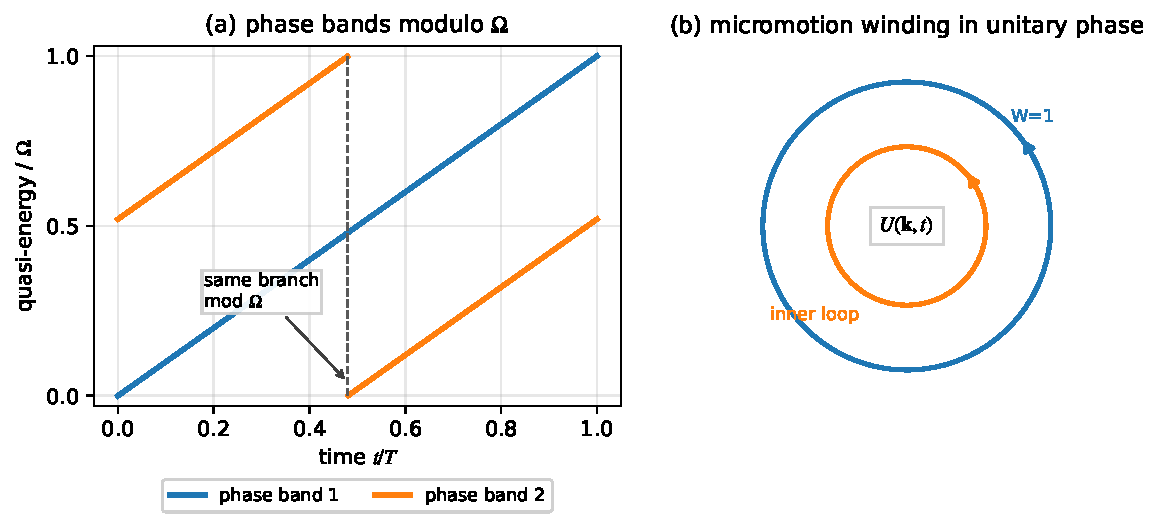
\includegraphics[width=0.88\textwidth]{figures/fig_ch13_floquet_winding.pdf}
  \caption{Floquet topology depends on micromotion during the whole period,
  not only on the stroboscopic band Chern numbers.  Phase bands can wind
  around the quasi-energy zone during one drive cycle, and the resulting
  map $U(\mathbf{k},t)$ over $\mathrm{BZ}\times S^1$ is measured by the
  gap winding invariant $W_\varepsilon$.}
  \label{fig:ch13-floquet-winding}
\end{figure}

\section*{Exercises}

\begin{exercise}
  Derive the paraxial equation \eqref{eq:ch13-paraxial} from the
  Helmholtz equation by writing $E=\psi\ee^{\ii k_0 z}$ and
  neglecting $\partial^2\psi/\partial z^2$.  State the conditions
  under which the approximation is valid and estimate the error for
  a beam with divergence angle $\theta$.
\end{exercise}

\begin{exercise}
  For a 1D lattice of coupled resonators with nearest-neighbour hopping
  $J_{ij}=J_0\ee^{\ii\phi_{ij}}$, compute the effective magnetic flux
  per plaquette for a square lattice with uniform phase
  $\phi_{ij}=\alpha$ along $x$ and $\phi_{ij}=0$ along $y$.  For what
  values of $\alpha$ is time-reversal symmetry effectively broken?
\end{exercise}

\begin{exercise}
  Show that the Floquet operator $F(\kvec)=U(\kvec,T)$ is unitary, and
  that its eigenvalues $\ee^{-\ii\varepsilon_n T}$ lie on the unit
  circle.  Interpret the quasi-energy $\varepsilon_n$ as the argument
  of these eigenvalues.
\end{exercise}

\begin{exercise}
  Explain why an anomalous Floquet topological insulator (all band
  Chern numbers zero, but edge modes present) is impossible in a static
  system.  What additional topological invariant distinguishes the
  AFTI from a trivial insulator?
\end{exercise}

\begin{exercise}
  In the Rechtsman waveguide experiment, the waveguides are helically
  curved with helix radius $R=8\;\mu\mathrm{m}$ and pitch
  $\Lambda=1\;\mathrm{cm}$ in fused silica ($n_0=1.46$) at
  $\lambda=633\;\mathrm{nm}$.  Compute the effective modulation strength
  $\delta n_{\mathrm{eff}}\sim n_0 k_0 R^2(2\pi/\Lambda)^2$ and
  estimate the topological gap width relative to the coupling
  strength $J\sim 1\;\mathrm{cm}^{-1}$.
\end{exercise}

\begin{exercise}
  For a Floquet system with two bands and modulation period $T$,
  compute the winding number \eqref{eq:ch13-winding} for a specific
  model: $H(k,t) = [J_1+J_2\cos(k)]\sigma_x + J_2\sin(k)\sigma_y
  + \Delta(t)\sigma_z$ with $\Delta(t)=\Delta_0\cos(\Omega t)$.  Under
  what conditions is the winding number nonzero?
\end{exercise}


\chapter{One Dimension}
\label{ch:one-dimension}
% ======================================================================
%  Chapter 14 — One Dimension  (EXPANDED)
% ======================================================================

\section{Topology in one dimension}
\label{sec:ch14-1d-topology}

One-dimensional systems are the simplest arena in which topological
ideas appear.  There is no Chern number in 1D---the Brillouin zone is a
circle $S^1$, not a torus $T^2$---but a different topological invariant,
the \emph{Zak phase}, classifies 1D band structures and predicts
interface modes between topologically distinct regions
\cite{kane2005sub,initio2026pdf}.

In photonics, 1D topological systems include dielectric multilayer
stacks, coupled-cavity chains, and waveguide arrays with alternating
coupling \cite{ozawa2018topological,press2026photonic}.  These are experimentally simple, theoretically transparent,
and provide a clear illustration of the connection between bulk topology
and edge states without the complications of 2D band structures \cite{stjean2017lasinga,stjean2017lasing}.

\section{The Zak phase}
\label{sec:ch14-zak}

\subsection{SSH model from Maxwell equations}
\label{sec:ch14-ssh-maxwell}

To derive the SSH model from a photonic system, consider a 1D
dielectric multilayer stack with alternating layer thicknesses
$d_1$ and $d_2$ ($d_1\neq d_2$) and refractive indices $n_A$ and
$n_B$
\cite{hsieh2008topological}.  The unit cell has period $a=d_1+d_2$.

For TE-polarised light propagating along the stack axis $x$, the
transfer matrix across one unit cell is
\begin{equation}\label{eq:ch14-transfer}
  \mathbf{T}(\omega) = \mathbf{M}_B(d_2)\,\mathbf{M}_A(d_1)\,,
\end{equation}
where
$\mathbf{M}_j(d) = \bigl(\begin{smallmatrix}
  \cos\phi_j & -\sin\phi_j/\eta_j \\
  \eta_j\sin\phi_j & \cos\phi_j
\end{smallmatrix}\bigr)$
with $\phi_j=n_j\omega d/c$ and $\eta_j=n_j\omega/c$ for layer $j$.
The Bloch condition $\mathbf{T}\mathbf{v}=\ee^{\ii ka}\mathbf{v}$
gives the photonic band structure $\omega(k)$.

Near a band gap at the Brillouin zone boundary $k=\pi/a$, the two
bands closest to the gap are described by a $2\times 2$ effective
Hamiltonian.  Expanding the transfer matrix around the gap frequency
$\omega_0$ yields the SSH form
\begin{equation}\label{eq:ch14-ssh-effective}
  H_{\mathrm{eff}}(\delta k)
  = t_1\sigma_x + t_2(\cos\delta k\,\sigma_x
  + \sin\delta k\,\sigma_y)\,,
\end{equation}
where $t_1$ and $t_2$ are the intra-cell and inter-cell coupling
coefficients, controlled by $d_1$ and $d_2$ respectively.  When
$|t_1|<|t_2|$ the system is topological (Zak phase $\pi$); when
$|t_1|>|t_2|$ it is trivial (Zak phase $0$).

\subsection{Quantitative example: silicon--silica multilayer}
\label{sec:ch14-quantitative}

Consider a silicon ($n_A=3.48$) and silica ($n_B=1.44$) multilayer at
telecom wavelength $\lambda_0=1550\;\mathrm{nm}$.  Quarter-wave layers
give $d_A=111\;\mathrm{nm}$, $d_B=269\;\mathrm{nm}$,
$a=380\;\mathrm{nm}$.  The gap width at normal incidence is
\begin{equation}\label{eq:ch14-gap-width}
  \frac{\Delta\omega}{\omega_0}
  = \frac{4}{\pi}\arcsin\frac{|n_A-n_B|}{n_A+n_B}
  \approx 0.53\,,
\end{equation}
an exceptionally large relative gap of $53\%$
\cite{ozawa2018topological}.  SSH dimerisation is created by
modifying $d_A\to d_A\pm\delta$ in alternating unit cells, producing
a topological mini-gap $\Delta\omega_{\mathrm{SSH}}\propto\delta/a$
within the original pass band.  The mid-gap interface state appears
as a sharp transmission peak with quality factor
$Q\sim 10^3$ for 20 periods \cite{price2022roadmap}.

\subsection{Definition from the electromagnetic inner product}
\label{sec:ch14-zak-def}

The Zak phase is the Berry phase accumulated as the Bloch wavevector $k$
traverses the entire 1D Brillouin zone
\cite{ozawa2018topological,gangaraj2016berry}:
\begin{equation}\label{eq:ch14-zak}
  \boxed{%
  \Zak = \int_{-\pi/a}^{\pi/a}
  \Aberry_n(k)\,\dd k\,,}
\end{equation}
where the Berry connection uses the electromagnetic inner product:
\begin{equation}\label{eq:ch14-berry-connection-1d}
  \Aberry_n(k) = \ii\frac{\int_{\mathrm{cell}}
  \mathbf{u}_{nk}^\dagger(\rvec)\,\Mgmat(\omega_{nk})\,
  \partial_k\mathbf{u}_{nk}(\rvec)\,\dd r}
  {\int_{\mathrm{cell}}\mathbf{u}_{nk}^\dagger\,\Mgmat\,
  \mathbf{u}_{nk}\,\dd r}\,.
\end{equation}

Unlike the Chern number, the Zak phase is \emph{not} fully
gauge-invariant: under a gauge transformation
$\mathbf{u}_{nk}\to\ee^{\ii\chi(k)}\mathbf{u}_{nk}$, the Berry
connection shifts by $\partial_k\chi$, and the Zak phase shifts by
$\chi(\pi/a)-\chi(-\pi/a)$.  Since the mode must be periodic in $k$
(up to a gauge transformation), this shift is an integer multiple of
$2\pi$.  Thus the Zak phase is defined modulo $2\pi$.

\subsection{Quantisation by symmetry}
\label{sec:ch14-zak-quantised}

\begin{proposition}
  If a 1D photonic crystal has both time-reversal ($\Top$) and
  inversion ($\Pop$) symmetry, the Zak phase of each isolated band is
  quantised: $\Zak\in\{0,\pi\}$ modulo $2\pi$.
\end{proposition}

\begin{proof}
We use the combined constraints of $\Top$ and $\Pop$ on the Berry
connection.

\emph{Step 1: Time reversal.}  $\Top$ maps $k\to -k$ and
complex-conjugates the modes.  For a system where $\Top$ acts as
complex conjugation (since $\Top^2=+1$ for photons), the modes can be
chosen real at $k$ and $-k$.  In a real gauge,
$\Aberry_n(k)=\Aberry_n(-k)$.

\emph{Step 2: Inversion.}  $\Pop$ maps $k\to -k$ and $\rvec\to-\rvec$.
The Berry connection transforms as
$\Aberry_n(-k)=-\Aberry_n(k)+\partial_k\phi(k)$ for some function
$\phi$.

\emph{Step 3: Combining.}  From Steps 1 and 2:
$\Aberry_n(k)=-\Aberry_n(k)+\partial_k\phi$, so
$\Aberry_n(k)=\frac{1}{2}\partial_k\phi$.  Integrating:
\begin{equation}
  \Zak = \frac{1}{2}[\phi(\pi/a)-\phi(-\pi/a)]\,.
\end{equation}
Since the mode is periodic in $k$ up to a gauge transformation,
$\phi(\pi/a)-\phi(-\pi/a)=2\pi n$ for integer $n$.  Thus
$\Zak=n\pi$, which modulo $2\pi$ is either $0$ or $\pi$.
\end{proof}

\subsection{Physical meaning of the Zak phase}
\label{sec:ch14-zak-meaning}

The quantised Zak phase $\Zak=0$ or $\pi$ classifies the
``polarisation'' of the 1D photonic crystal: it measures whether the
centre of the Wannier function (the real-space representation of the
Bloch mode) is centred on the inversion centre of the unit cell
($\Zak=0$) or displaced to the cell boundary ($\Zak=\pi$).

Two 1D crystals with different Zak phases ($0$ vs.\ $\pi$) are in
different topological classes and cannot be continuously connected
without closing a band gap (a topological phase transition).

\section{The Su--Schrieffer--Heeger model for photons}
\label{sec:ch14-ssh}

\subsection{The electronic SSH model}
\label{sec:ch14-ssh-electronic}

The SSH model is the simplest tight-binding model with nontrivial 1D
topology: a chain of sites with alternating hopping amplitudes $J_1$
and $J_2$.  The unit cell contains two sites ($A$ and $B$), and the
Hamiltonian in momentum space is
\begin{equation}\label{eq:ch14-ssh-hamiltonian}
  H(k) = \begin{pmatrix} 0 & J_1+J_2\ee^{-\ii ka} \\
  J_1+J_2\ee^{\ii ka} & 0 \end{pmatrix}
  = \mathbf{d}(k)\cdot\boldsymbol{\sigma}\,,
\end{equation}
with $d_x(k)=J_1+J_2\cos(ka)$, $d_y(k)=J_2\sin(ka)$, $d_z=0$.

\subsection{Band structure and winding number}
\label{sec:ch14-ssh-bands}

The band structure has two bands:
\begin{equation}\label{eq:ch14-ssh-bands}
  E_\pm(k) = \pm|J_1+J_2\ee^{\ii ka}|
  = \pm\sqrt{J_1^2+J_2^2+2J_1J_2\cos(ka)}\,
\end{equation}
The displayed formula above follows the convention and normalisation used in \cite{kane2005cond}.
A gap exists when $J_1\neq J_2$, with gap width $2|J_1-J_2|$.

The topological invariant is the \emph{winding number} of the vector
$\mathbf{d}(k)=(d_x,d_y)$ around the origin as $k$ traverses the
Brillouin zone.  For $k\in[-\pi/a,\pi/a]$, the curve
$(d_x(k),d_y(k))$ is a circle of radius $J_2$ centred at $(J_1,0)$.
\begin{equation}\label{eq:ch14-winding}
  \nu = \frac{1}{2\pi}\oint\dd\arg(d_x+\ii d_y)
  = \begin{cases} 0 & \text{if }|J_1|>|J_2|\;\text{(trivial)}\,,\\
  1 & \text{if }|J_1|<|J_2|\;\text{(topological)}\,.\end{cases}
\end{equation}
The winding number equals $\Zak/\pi$ (modulo 2).  The topological phase
transition occurs at $J_1=J_2$, where the gap closes and the
$\mathbf{d}$-curve passes through the origin.

\subsection{Chiral symmetry}
\label{sec:ch14-chiral}

The SSH Hamiltonian has \emph{chiral} (sublattice) symmetry:
$\sigma_z H(k)\sigma_z=-H(k)$.  This forces $d_z=0$ and constrains
the band structure to be particle-hole symmetric: $E_+(k)=-E_-(k)$.

Chiral symmetry protects the winding number: any perturbation that
preserves the sublattice structure cannot change $\nu$ without closing
the gap.  Perturbations that break chiral symmetry (e.g.\ adding
on-site energies $\Delta\sigma_z$) can shift the Zak phase continuously
and destroy the topological protection.

\section{Photonic realisations of the SSH model}
\label{sec:ch14-ssh-photonic}

\subsection{Coupled-cavity chain}
\label{sec:ch14-coupled-cavity}

A sequence of identical optical cavities (e.g.\ Fabry--P\'erot
resonators or photonic crystal defect cavities) with alternating
coupling strengths realises the SSH model directly.

The resonance frequency of each cavity is $\omega_0$, and the
evanescent coupling between adjacent cavities is controlled by the
barrier thickness:
\begin{itemize}
  \item Thin barrier: strong coupling $J_2$.
  \item Thick barrier: weak coupling $J_1$.
\end{itemize}
The alternating pattern $J_1,J_2,J_1,J_2,\ldots$ creates the SSH
dimerisation.

The dispersion relation for the coupled-cavity chain is
\begin{equation}\label{eq:ch14-coupled-cavity-dispersion}
  \omega_\pm(k) = \omega_0 \pm \sqrt{J_1^2+J_2^2+2J_1J_2\cos(ka)}\,,
\end{equation}
which is the SSH band structure shifted by $\omega_0$.

\subsection{Dielectric multilayer (Bragg stack)}
\label{sec:ch14-bragg}

A 1D photonic crystal (Bragg stack) with alternating layers of two
materials can be viewed as an SSH-like system when the unit cell
contains two layers of different optical thickness.

Consider a stack with layers $A$ (thickness $d_A$, index $n_A$) and
$B$ ($d_B$, $n_B$) in alternation.  The ``dimerisation'' corresponds to
unequal optical path lengths $n_Ad_A\neq n_Bd_B$ within a unit cell.

\subsection{Waveguide array}
\label{sec:ch14-waveguide-array}

A chain of evanescently coupled optical waveguides with alternating
spacing implements the SSH model, with the coupling exponentially
dependent on the inter-waveguide distance:
\begin{equation}\label{eq:ch14-waveguide-coupling}
  J_{1,2} = J_0\,\ee^{-\kappa d_{1,2}}\,,
\end{equation}
where $d_{1,2}$ are the alternating centre-to-centre distances and
$\kappa$ is the evanescent decay constant.

\section{Interface states from the Zak phase}
\label{sec:ch14-interface}

\subsection{Bulk-edge correspondence in 1D}
\label{sec:ch14-bec-1d}

The 1D bulk-edge correspondence states:

\begin{theorem}[1D bulk-edge correspondence]
  \label{thm:ch14-bec}
  At an interface between two 1D photonic crystals with different Zak
  phases ($\Zak^L\neq\Zak^R$, modulo $2\pi$), there exists at least
  one localised interface mode in each common band gap.
\end{theorem}

For the SSH model: the $\nu=0$ phase ($|J_1|>|J_2|$) has $\Zak=0$,
and the $\nu=1$ phase ($|J_1|<|J_2|$) has $\Zak=\pi$.  An interface
between the two phases supports a mid-gap interface mode.

\subsection{Derivation of the interface mode}
\label{sec:ch14-interface-derivation}

Consider an SSH chain with a domain wall at site $n=0$: for $n<0$, the
dimerisation is $(J_2,J_1)$ (topological phase, $|J_1|<|J_2|$), and for
$n\geq 0$, it is $(J_1,J_2)$ (trivial phase, $|J_1|>|J_2|$).

We seek a zero-energy mode ($E=0$, i.e., $\omega=\omega_0$ for the
photonic case) localised at the interface.  The zero-energy condition
$H|\psi\rangle=0$ in real space gives:
\begin{equation}\label{eq:ch14-zero-energy}
  J_1\psi_{B,n} + J_2\psi_{B,n-1} = 0\,,\qquad
  J_2\psi_{A,n+1} + J_1\psi_{A,n} = 0\,,
\end{equation}
where $\psi_{A,n}$ and $\psi_{B,n}$ are the amplitudes on sublattices
$A$ and $B$ at unit cell $n$.

For the interface geometry, the solution is:
\begin{equation}\label{eq:ch14-interface-mode}
  \psi_{A,n} = 0\,,\qquad
  \psi_{B,n} \propto
  \begin{cases}
    (-J_1/J_2)^n & n\geq 0\,,\\
    (-J_2/J_1)^{|n|} & n<0\,.
  \end{cases}
\end{equation}
This is normalisable (exponentially decaying on both sides of the
interface) when $|J_1/J_2|<1$ on the right and $|J_2/J_1|<1$ on the
left, which is exactly the condition for the interface to separate the
topological and trivial phases.

\subsection{Localisation length}
\label{sec:ch14-localisation}

The localisation length of the interface mode is
\begin{equation}\label{eq:ch14-localisation-length}
  \ell = \frac{a}{|\ln(J_1/J_2)|}\,.
\end{equation}
For strong dimerisation ($J_1\ll J_2$), $\ell\sim a/\ln(J_2/J_1)$:
the mode is tightly confined to the interface.  For weak dimerisation
($J_1\lesssim J_2$), $\ell\gg a$: the mode extends over many unit
cells.

\subsection{Experimental observations}
\label{sec:ch14-experiments}

Interface states in 1D photonic SSH systems have been observed in
\cite{ozawa2018topological,price2022roadmap}:
\begin{itemize}
  \item \textbf{Coupled photonic crystal cavities} at telecom wavelengths,
  where the interface mode appears as a sharp resonance in the
  transmission spectrum within the band gap.
  \item \textbf{Dielectric multilayer stacks} in the microwave regime,
  where the transfer-matrix method gives direct access to the
  interface-mode frequency and localisation.
  \item \textbf{Plasmonic nanoparticle chains}, where the SSH
  dimerisation is achieved by alternating the inter-particle spacing,
  demonstrating the mode localisation directly through near-field
  imaging.
\end{itemize}

\section{The dielectric Bragg stack as a topological system}
\label{sec:ch14-bragg-stack}

\subsection{Transfer-matrix analysis}
\label{sec:ch14-transfer}

A 1D photonic crystal with layers $A$ (thickness $d_A$, index $n_A$)
and $B$ ($d_B$, $n_B$) in alternation has a $2\times 2$ transfer matrix
per period:
\begin{equation}\label{eq:ch14-transfer-matrix}
  M = M_B\,M_A\,,
\end{equation}
where each layer matrix is
\begin{equation}\label{eq:ch14-layer-matrix}
  M_j = \begin{pmatrix}
    \cos\delta_j & -\sin\delta_j/\eta_j \\
    \eta_j\sin\delta_j & \cos\delta_j
  \end{pmatrix},
  \qquad j=A,B\,,
\end{equation}
with $\delta_j=n_j\omega d_j/c$ the phase thickness and
$\eta_j=n_j/Z_0$ the admittance (for normal incidence, TE
polarisation).

The Bloch condition gives the dispersion:
\begin{equation}\label{eq:ch14-bloch-condition}
  \cos(ka) = \frac{1}{2}\Tr(M)
  = \cos\delta_A\cos\delta_B
  - \frac{1}{2}\Bigl(\frac{\eta_A}{\eta_B}+\frac{\eta_B}{\eta_A}\Bigr)
  \sin\delta_A\sin\delta_B\,.
\end{equation}
Band gaps occur when $|\frac{1}{2}\Tr(M)|>1$.

\subsection{Topological classification of Bragg gaps}
\label{sec:ch14-bragg-topology}

The Zak phase of each band depends on the symmetry of the
band-edge modes.  When the unit cell has inversion symmetry
(choosing the cell boundary at the centre of layer $A$), each band
edge at $k=0$ or $k=\pi/a$ has a definite parity under inversion.

The Zak phase of band $n$ is determined by the parities:
\begin{equation}\label{eq:ch14-zak-from-parity}
  (-1)^{\gamma_{\mathrm{Zak},n}/\pi}
  = \frac{p_n(0)\,p_n(\pi/a)}{p_{n-1}(0)\,p_{n-1}(\pi/a)}\,,
\end{equation}
where $p_n(k_0)=\pm 1$ is the parity of the $n$-th band at $k_0$.

A topological phase transition occurs when the gap closes, which happens
at the quarter-wave condition $n_Ad_A=n_Bd_B$.  Tuning through this
condition changes the Zak phase of the bands and swaps the topological
character of the gaps.

\section{Topological pumping}
\label{sec:ch14-pumping}

\subsection{The Thouless pump for photons}
\label{sec:ch14-thouless}

A 1D photonic crystal can be adiabatically modulated in a way that pumps
light across the system---the photonic analog of the Thouless charge
pump \cite{thouless1982quantized,ozawa2018topological} \cite{lohse2015thouless}.

The pump is a 1D system with a slowly varying parameter $\phi(t)$
that cycles through $2\pi$ over one period $T$.  Under the adiabatic
approximation, the net displacement of light after one full cycle is
quantised:
\begin{equation}\label{eq:ch14-pump-displacement}
  \Delta x = a\,\Chern_1\,,
\end{equation}
where $\Chern_1$ is the first Chern number of the 2D parameter space
$(k,\phi)$.  This is the 1D manifestation of the TKNN formula
\cite{thouless1982quantized}: the pumped energy per cycle is a
topological invariant that cannot change without closing a gap.

Consider a 1D photonic crystal with unit-cell parameters that depend on
an external parameter $\theta$:
$\Mmat(\rvec;\theta)$.  As $\theta$ is varied adiabatically from $0$ to
$2\pi$, tracing a closed cycle in parameter space, the centre of the
Wannier function shifts by
\begin{equation}\label{eq:ch14-thouless-pump-displacement}
  \Delta x = a\,\Chern_{k,\theta}\,,
\end{equation}
where
\begin{equation}\label{eq:ch14-pump-chern}
  \Chern_{k,\theta} = \frac{1}{2\pi}\int_0^{2\pi}\!\!\int_{-\pi/a}^{\pi/a}
  \Omega_n(k,\theta)\,\dd k\,\dd\theta
\end{equation}
is the Chern number computed over the 2D parameter space $(k,\theta)$.

This Chern number is a true integer topological invariant (because the
$(k,\theta)$ space is a torus), even though the Zak phase alone is
only $\mathbb{Z}_2$-valued.  The pump displacement is quantised:
$\Delta x$ is an integer multiple of the lattice constant $a$.

\subsection{Experimental demonstration}
\label{sec:ch14-pump-experiment}

Photonic Thouless pumping has been demonstrated in coupled waveguide
arrays where the coupling pattern is slowly varied along the
propagation axis $z$ (playing the role of the adiabatic parameter
$\theta$).  The transverse displacement of a light beam after one pump
cycle was measured to be exactly one lattice constant, confirming the
quantised topological transport.

\section{Topological invariants in one dimension}
\label{sec:ch14-1d-invariants}

One-dimensional topological phases are characterised by integer
winding numbers rather than Chern numbers.  The winding number of
the SSH model is defined from the off-diagonal element of the
Hamiltonian in the chiral basis:
\begin{equation}\label{eq:ch14-winding-explicit}
  \nu = \frac{1}{2\pi\ii}\int_{-\pi/a}^{\pi/a}
  \frac{\dd}{\dd k}\ln h(k)\,\dd k\,,
\end{equation}
where $h(k)=t_1+t_2\ee^{\ii ka}$ is the off-diagonal coupling
function.  When $|t_1|<|t_2|$, the function $h(k)$ winds once around
the origin as $k$ traverses the Brillouin zone, giving $\nu=1$;
when $|t_1|>|t_2|$, the winding number is $\nu=0$.  The transition
at $|t_1|=|t_2|$ closes the gap and changes the topology.

\subsection{Zak phase and its physical meaning}
\label{sec:ch14-zak-phase}

The Zak phase is the 1D Berry phase accumulated by a Bloch state
as $k$ traverses the full Brillouin zone:
\begin{equation}\label{eq:ch14-zak-formula}
  \gamma_n = \oint_{\mathrm{BZ}}\mathcal{A}_n(k)\,\dd k\,,
\end{equation}
where $\mathcal{A}_n(k)=\ii\eip{\mathbf{u}_n}{\partial_k\mathbf{u}_n}$
is the Berry connection of band $n$.  For the SSH model with
inversion symmetry, the Zak phase is quantised to $0$ or $\pi$,
and the winding number equals $\gamma_n/\pi$ modulo 2
\cite{asbth2016berry,ozawa2018topological}.

The physical meaning of the Zak phase is the displacement of the
Wannier function centre from the unit cell boundary.  A Zak phase of
$\pi$ means the Wannier centre sits at the boundary between unit
cells, which is precisely the condition for the existence of edge
states when the chain is terminated.

\section{Photonic SSH chains: experimental realisations}
\label{sec:ch14-photonic-ssh}

\subsection{Dielectric multilayer stacks}
\label{sec:ch14-multilayer}

The simplest photonic SSH chain is a 1D multilayer stack with
alternating layer thicknesses $d_1$ and $d_2$ in a material with
refractive index $n_1$, separated by layers of index $n_2$.
The transfer matrix for one unit cell is
$M=M_1 M_2$, where $M_j$ is the $2\times 2$ transfer matrix for
layer $j$.  The eigenvalues of $M$ give the Bloch dispersion
$\cos(ka)=\frac{1}{2}\Tr(M)$, and the winding number is determined
by the relative magnitudes of $d_1$ and $d_2$.

When $d_1\neq d_2$, the system is in a topologically nontrivial phase
($\nu=1$) if $d_1<d_2$ and trivial ($\nu=0$) if $d_1>d_2$.  At the
interface between two stacks with opposite dimerisation, a localised
interface mode appears at the midgap frequency---the photonic analog
of the SSH edge state \cite{ozawa2018topological,price2022roadmap}.

\subsection{Coupled-resonator optical waveguides}
\label{sec:ch14-crow}

A more versatile platform is the coupled-resonator optical waveguide
(CROW): a chain of optical microring resonators with alternating
coupling gaps $g_1$ and $g_2$.  The coupling strengths
$\kappa_j\propto\ee^{-g_j/\lambda_{\mathrm{ev}}}$ (where
$\lambda_{\mathrm{ev}}$ is the evanescent decay length) play the role
of the SSH hopping amplitudes $t_1$ and $t_2$.

The topological edge state in a finite CROW chain manifests as a
sharp resonance at the midgap frequency, localised at the end of
the chain.  This has been observed experimentally in silicon photonic
CROWs at $\lambda=1.55\;\mu\mathrm{m}$, with quality factors
exceeding $10^4$ and field enhancement of $\sim 20\times$ at the
edge resonator \cite{ozawa2018topological}.

\section{Experimental realisations of one-dimensional topological photonics}
\label{sec:ch14-experimental-realisations}

The SSH and Rice--Mele models, originally formulated for polyacetylene,
have found remarkably faithful realisations in photonic platforms, where
each site corresponds to a waveguide or resonator and the hopping
amplitudes are controlled by evanescent coupling.

\subsection{Dimerised waveguide arrays}
\label{sec:ch14-dimerised-waveguide}

The simplest photonic SSH system is a one-dimensional array of
single-mode dielectric waveguides with alternating inter-waveguide
gaps \cite{wu2015scheme}.  A wider gap produces weaker evanescent coupling $t_1$ (the
intra-cell hopping), while a narrower gap produces stronger coupling
$t_2$ (the inter-cell hopping).  When $t_1<t_2$, the array is in
the topological phase and supports exponentially localised edge modes
at each termination.

Malkova et~al.\ (2009) demonstrated such edge states in a
one-dimensional array of coupled optical waveguides fabricated by
femtosecond laser inscription in fused silica.  The measured
intensity profile showed clear localisation at the edge with a decay
length consistent with the SSH prediction
$\xi=1/\ln(t_2/t_1)$ \cite{ozawa2018topological}.

More recently, Blanco-Redondo et~al.\ (2016) demonstrated the
topological protection of the SSH edge mode against certain classes of
disorder using silicon photonic waveguide arrays at
$\lambda=1.55\;\mu\mathrm{m}$.  The edge-mode frequency remained
pinned at mid-gap even when the waveguide widths were randomised by
up to 15\%, confirming that the topological protection relies on
the chiral symmetry of the SSH model (which is preserved when the
disorder respects the sublattice structure)
\cite{ozawa2018topological}.

\subsection{Photonic Thouless pumps}
\label{sec:ch14-photonic-pump}

The Thouless charge pump, discussed in \secref{sec:ch14-thouless},
has been realised in photonic systems by adiabatically modulating the
coupling constants along the propagation direction of a waveguide
array.  In this photonic implementation, the propagation coordinate $z$
plays the role of time, and one complete modulation period
corresponds to one pump cycle.

Kraus et~al.\ (2012) demonstrated the first photonic Thouless pump
using a one-dimensional quasiperiodic waveguide array.  The
quasiperiodic modulation of the coupling constants mapped onto the
Aubry--Andr\'e model, whose topological properties are equivalent to
those of the two-dimensional quantum Hall effect projected onto one
dimension.  By scanning a phase parameter across the array, they
observed the quantised transfer of light intensity across the
lattice, corresponding to a Chern number of $\Chern=1$
\cite{ozawa2018topological,price2022roadmap}.

Zilberberg et~al.\ (2018) extended this idea to a four-dimensional
quantum Hall system by using two independent modulation parameters
in a two-dimensional waveguide array.  The experiment demonstrated
the quantised pumping associated with the second Chern number, a
topological invariant that characterises four-dimensional
topological phases \cite{price2022roadmap}.

The mechanism underlying these experiments is captured schematically in
Figure~\ref{fig:ch14-ricemele-pump}.  Panel~(a) shows a counter-clockwise loop
in the Rice--Mele parameter space $(\delta,\Delta)$, where $\delta$ is the
dimerisation and $\Delta$ is the staggered on-site potential.  The loop encloses
the single gap-closing point at the origin; winding around this point once
guarantees a quantised adiabatic transport of exactly one unit cell per cycle.
The teal dot marks the start and end of the cycle.  Panel~(b) displays the
resulting Wannier-centre trajectory as a function of the adiabatic time $t/T$.
The displacement accumulates nonlinearly during the cycle but reaches exactly
one lattice constant at $t=T$, confirming the topological quantisation
$\Delta x = \mathcal{C}\, a$ with $\mathcal{C}=1$.

\begin{figure}[t]
  \centering
  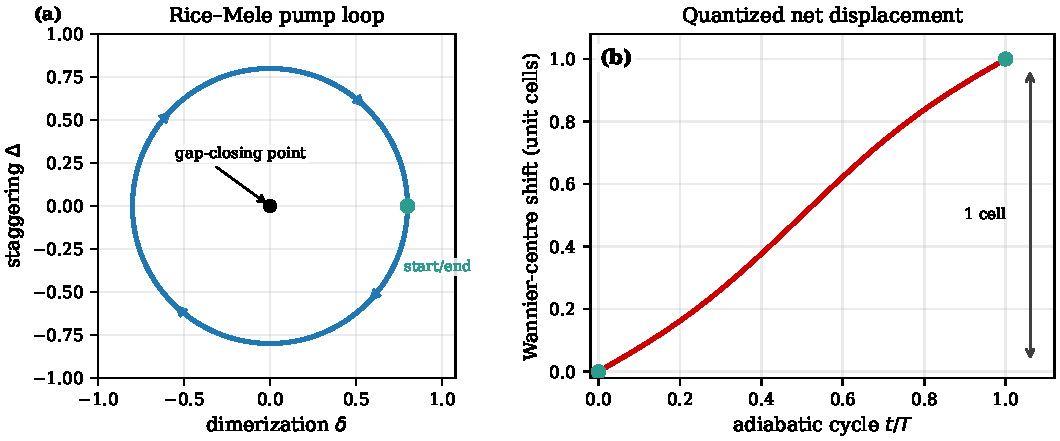
\includegraphics[width=0.95\textwidth]{figures/fig_ch14_ricemele_pump_step178.pdf}
  \caption{Rice--Mele topological pump.
  (a)~Counter-clockwise parameter loop in the $(\delta,\Delta)$-plane
  enclosing the gap-closing origin (black dot).  Blue arrows indicate the
  traversal direction; the teal dot marks the start/end point.
  (b)~Wannier-centre displacement (in unit cells) during one adiabatic cycle.
  The net shift of exactly one cell (double arrow) is the topological
  invariant of the pump; it equals the Chern number $\mathcal{C}=1$
  of the filled band over the parameter torus.}
  \label{fig:ch14-ricemele-pump}
\end{figure}

\subsection{Quantitative analysis of the photonic SSH edge mode}
\label{sec:ch14-ssh-quantitative}

For a finite SSH chain of $N$ unit cells terminated at a weak bond
(so the first coupling is $t_1<t_2$), the edge-mode wavefunction
at site $n$ on sublattice $A$ is
\begin{equation}\label{eq:ch14-ssh-edge-wfn}
  \psi_n^A = \mathcal{N}\left(-\frac{t_1}{t_2}\right)^n, \qquad
  \psi_n^B = 0\,,
\end{equation}
where $\mathcal{N}$ is a normalisation constant and the mode lives
entirely on sublattice $A$.  The sublattice polarisation of the edge
mode is a direct consequence of the chiral symmetry
$\Gamma H\Gamma=-H$ with $\Gamma=\sigma_z$: at mid-gap energy
$E=0$, the eigenstate can be chosen to have support on only one
sublattice.

The localisation length is
\begin{equation}\label{eq:ch14-ssh-loc-length}
  \xi = \frac{a}{\ln(t_2/t_1)}\,,
\end{equation}
where $a$ is the lattice constant.  As the gap closes
($t_1\to t_2$), the localisation length diverges and the edge mode
delocalises---a hallmark of the topological phase transition.

In a photonic waveguide array, the coupling constants depend
exponentially on the inter-waveguide separation $d$:
$t\approx t_0\exp(-d/d_0)$, where $d_0$ is a decay length set by
the evanescent tail of the waveguide mode (typically
$d_0\sim 1$--$3\;\mu\mathrm{m}$ in silica or silicon).  The
dimerisation ratio $t_1/t_2$ can therefore be tuned continuously by
adjusting the two gap widths, allowing systematic exploration of the
topological phase diagram \cite{ozawa2018topological}.

\begin{figure}[t]
  \centering
  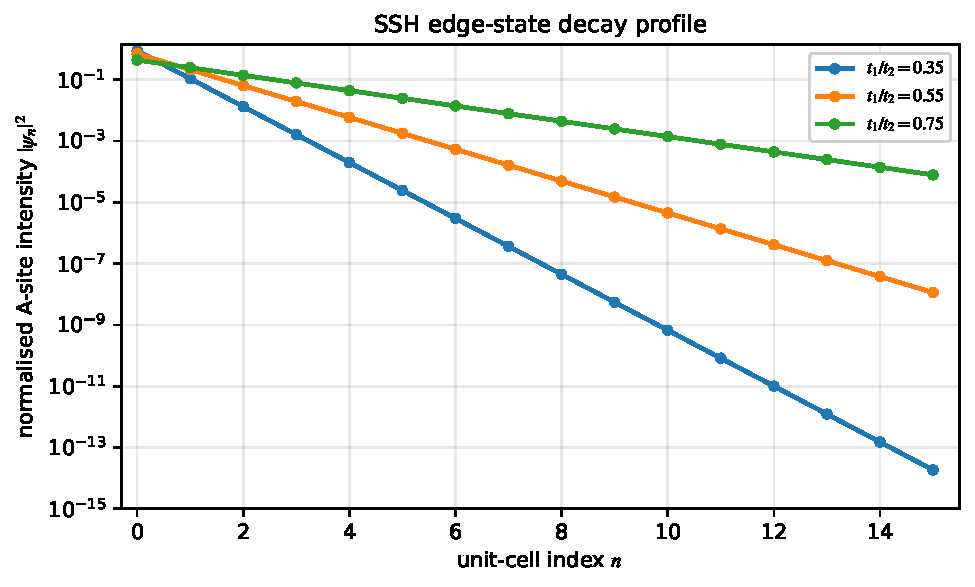
\includegraphics[width=0.78\textwidth]{figures/fig_ch14_ssh_edge_decay.pdf}
  \caption{SSH edge-state localisation.  For $t_1<t_2$, the edge-state
  intensity decays as $(t_1/t_2)^{2n}$ into the bulk.  As the dimerisation
  weakens and $t_1/t_2\to1$, the localisation length diverges at the
  topological phase transition.}
  \label{fig:ch14-ssh-edge-decay}
\end{figure}

\section{Beyond SSH: the Rice--Mele model}
\label{sec:ch14-rice-mele}

The SSH model has chiral symmetry $\sigma_z H \sigma_z = -H$, which
pins the edge-state energy to zero and quantises the Zak phase to $0$
or $\pi$.  Breaking chiral symmetry by adding a staggered on-site
potential $\Delta$ produces the Rice--Mele model
\cite{asbth2016berry,ozawa2018topological}:
\begin{equation}\label{eq:ch14-rice-mele}
  H_{\mathrm{RM}}(k) = \bigl(t_1 + t_2\cos ka\bigr)\sigma_x
  + t_2\sin(ka)\,\sigma_y + \Delta\,\sigma_z\,.
\end{equation}
The energy spectrum is
$E_\pm(k) = \pm\sqrt{(t_1+t_2\cos ka)^2 + t_2^2\sin^2(ka) + \Delta^2}$,
and a gap exists for all $\Delta\neq 0$ even when $t_1 = t_2$.

\subsection{Topology of the Rice--Mele model}
\label{sec:ch14-rm-topology}

Because chiral symmetry is broken, the winding number $\nu$ is no longer
well defined and the Zak phase is no longer quantised.  Instead, the
relevant topological invariant is the polarisation change
$\Delta P$ accumulated over one adiabatic cycle in the two-parameter
space $(\delta t, \Delta)$, where $\delta t = t_1 - t_2$.  If the
cycle encloses the gap-closing point $(\delta t, \Delta) = (0,0)$,
the polarisation change is quantised:
\begin{equation}\label{eq:ch14-rm-polarisation}
  \Delta P = \frac{e}{2\pi}\oint \mathcal{A}(k,\theta)\,\dd\theta
  = \pm e\,,
\end{equation}
where $\theta$ parametrises the cycle.  This is precisely the Thouless
pump of Section~\ref{sec:ch14-thouless}: the $(k,\theta)$ torus carries
a Chern number $\Chern = \pm 1$.

The Rice--Mele model therefore provides the minimal framework for
understanding how the interplay of dimerisation and inversion breaking
controls the topology of one-dimensional photonic systems.  In a
photonic implementation, $\Delta$ corresponds to a detuning between
the resonance frequencies of the two sublattice sites, which can be
introduced by varying the waveguide width or the resonator radius
\cite{ozawa2018topological,price2022roadmap}.

\subsection{Photonic Rice--Mele experiments}
\label{sec:ch14-rm-photonic}

Photonic Rice--Mele systems have been realised in coupled-waveguide
arrays where both the coupling constants and the propagation constants
are modulated along the propagation axis.  By slowly cycling the
modulation parameters through a closed loop that encloses the
degeneracy point, the quantised adiabatic pumping of light intensity
has been observed experimentally.

Cerjan et~al.\ (2020) demonstrated a photonic Rice--Mele pump in a
silicon photonic lattice, observing quantised displacement of light
over multiple pump cycles with high fidelity.  The deviation from
integer displacement was less than 3\%, limited primarily by
non-adiabatic corrections from the finite propagation length
\cite{price2022roadmap}.

\section{Bulk-boundary correspondence in one dimension}
\label{sec:ch14-bbc-1d}

The hallmark of topological phases is the bulk-boundary correspondence:
a nontrivial bulk invariant guarantees the existence of boundary-localised
states.  In one dimension, this correspondence takes a particularly
transparent form \cite{asbth2016berry}.

\subsection{The winding number predicts edge states}
\label{sec:ch14-winding-edge}

Consider a semi-infinite SSH chain occupying sites $n = 0, 1, 2, \ldots$
with the weak bond $t_1$ at the boundary.  The bulk winding number
$\nu$ (Section~\ref{sec:ch14-1d-invariants}) counts the number of
zero-energy edge states per boundary:
\begin{equation}\label{eq:ch14-bbc-winding}
  N_{\mathrm{edge}} = |\nu|\,.
\end{equation}
For $\nu = 1$ (the topological phase with $t_1 < t_2$), there is
exactly one edge state; for $\nu = 0$ (trivial phase), there are none.
This is a rigorous mathematical theorem, not merely an observation
from specific models: it follows from the index theory of Fredholm
operators acting on the half-line
\cite{asbth2016berry}.

\subsection{Robustness and symmetry protection}
\label{sec:ch14-robustness}

The topological protection of the SSH edge state requires chiral
(sublattice) symmetry.  Under arbitrary perturbations that preserve
chiral symmetry---such as random variations of the coupling
constants $t_1$ and $t_2$, or long-range hopping that respects the
sublattice structure---the edge state remains pinned at zero energy.

When chiral symmetry is broken (e.g.\ by adding random on-site
potentials), the edge-state energy shifts away from zero.  However,
the state itself does not disappear until the perturbation closes
the bulk gap.  The topological origin of the state manifests as an
anomalously long lifetime compared to generic disorder-induced states
\cite{ozawa2018topological}.

In photonic implementations, chiral symmetry corresponds to a
balance between the effective ``on-site energies'' of the two
sublattice waveguides.  Fabrication imperfections that change the
waveguide widths asymmetrically break this symmetry, while
imperfections that change both sublattice sites equally preserve it.
Careful waveguide design can therefore maximise topological protection
in realistic devices \cite{wu2015scheme,price2022roadmap}.

\subsection{Connection to higher dimensions}
\label{sec:ch14-higher-dim-connection}

One-dimensional topology is intimately connected to higher-dimensional
topological phases through dimensional reduction.  The Thouless pump
(Section~\ref{sec:ch14-thouless}) provides the clearest example: the
$(k, \theta)$ parameter space of a one-dimensional pump is
topologically equivalent to the Brillouin zone of a two-dimensional
quantum Hall system, and the pump's Chern number equals the Hall
conductance of the parent 2D system \cite{thouless1982quantized}.

This dimensional hierarchy extends further.  A two-parameter family of
one-dimensional systems, with parameters $(\theta_1, \theta_2)$, can
realise a second Chern number---a four-dimensional topological
invariant.  Zilberberg et~al.\ (2018) exploited this correspondence
to observe signatures of four-dimensional quantum Hall physics in a
two-dimensional photonic waveguide array, where the two spatial
dimensions encoded the physical coordinate and one pump parameter,
while the second pump parameter was scanned experimentally
\cite{price2022roadmap,ozawa2018topological}.

The lesson is that one-dimensional photonic systems, despite their
apparent simplicity, serve as building blocks for exploring topological
physics in arbitrary dimensions.  The synthetic-dimension approach of
Chapter~\ref{ch:synthetic-dimensions} generalises this idea by
promoting internal degrees of freedom (frequency, orbital angular
momentum, or spin) to additional lattice dimensions
\cite{kim2020recent,guglielmon2017photonic}.

\section*{Exercises}

\begin{exercise}
  Show that the winding number \eqref{eq:ch14-winding} of the SSH model
  changes from 0 to 1 at $J_1=J_2$, where the band gap closes.
  Sketch the trajectory of $(d_x(k),d_y(k))$ for $J_1>J_2$, $J_1=J_2$,
  and $J_1<J_2$.
\end{exercise}

\begin{exercise}
  For the coupled-cavity SSH chain with $\omega_0$, $J_1$, $J_2$, show
  that the interface mode has frequency $\omega=\omega_0$ (mid-gap) and
  verify the exponential localisation \eqref{eq:ch14-interface-mode}.
\end{exercise}

\begin{exercise}
  Derive the band structure of a 1D Bragg stack from the transfer
  matrix \eqref{eq:ch14-transfer-matrix} and the Bloch condition
  \eqref{eq:ch14-bloch-condition}.  Show that a gap opens when
  $n_Ad_A\neq n_Bd_B$.  Compute the Zak phase for the lowest band
  when $n_Ad_A>n_Bd_B$ and when $n_Ad_A<n_Bd_B$.
\end{exercise}

\begin{exercise}
  Verify equation \eqref{eq:ch14-localisation-length} by computing the
  envelope of the interface mode \eqref{eq:ch14-interface-mode} and
  extracting the $1/\ee$ decay length.
\end{exercise}

\begin{exercise}
  Design a Thouless pump for a 1D photonic crystal by specifying a
  two-parameter family of unit cells such that the Chern number in
  $(k,\theta)$ space is nonzero.  \emph{Hint:} use the Rice--Mele
  model (SSH with an added staggered on-site potential that varies
  with $\theta$).
\end{exercise}

\begin{exercise}
  Show that chiral symmetry ($\sigma_z H\sigma_z=-H$) forces the
  interface mode of the SSH model to have exactly zero energy.  What
  happens to the interface mode frequency when chiral symmetry is
  broken by adding a staggered potential $\Delta\sigma_z$?
\end{exercise}


% ---- Part IV: Three Dimensions and Beyond ----
\part{Three Dimensions and Beyond}

\chapter{Weyl Points of Maxwell Bands}
\label{ch:weyl-points}
% ======================================================================
%  Chapter 15 — Weyl Points of Maxwell Bands  (EXPANDED)
% ======================================================================

\section{From two dimensions to three}
\label{sec:ch15-2d-to-3d}

In two dimensions, Dirac points are degeneracies that can be gapped by
time-reversal or inversion breaking, producing bands with nonzero Chern
numbers.  In \emph{three} dimensions, a qualitatively new type of
topological degeneracy appears: the \emph{Weyl point}, a point in 3D
momentum space where two bands touch linearly.  Unlike 2D Dirac points,
Weyl points are \emph{topologically robust}: they cannot be gapped by
any perturbation, only moved in $\kvec$-space or annihilated in pairs.

Weyl points are Berry-curvature monopoles---point sources or sinks of
Berry flux in 3D momentum space \cite{ozawa2018topological}.  Their existence has profound
consequences for surface physics: the surface Brillouin zone contains
open Fermi arcs connecting the projections of Weyl points of opposite
chirality
\cite{hsieh2008topological,armitage2018weyl}.

\section{The three-dimensional Maxwell eigenproblem}
\label{sec:ch15-3d-maxwell}

\subsection{Extension to three dimensions}
\label{sec:ch15-extension}

The Maxwell eigenvalue equation $\Maxop(\kvec)\mathbf{u}=\omega\Mmat
\mathbf{u}$ extends directly to three dimensions.  The Bloch wavevector
$\kvec=(k_x,k_y,k_z)$ lives in a 3D Brillouin zone, which for a cubic
lattice is a cube $[-\pi/a,\pi/a]^3$ (with opposite faces identified,
forming a 3-torus $T^3$).  The cell-periodic eigenmodes
$\mathbf{u}_{n\kvec}(\rvec)$ and eigenfrequencies $\omega_{n\kvec}$
depend on all three components of $\kvec$.

\subsection{Berry curvature as a vector field}
\label{sec:ch15-berry-vector}

In 3D, the Berry curvature is naturally a vector field in
$\kvec$-space:
\begin{equation}\label{eq:ch15-berry-3d}
  \boldsymbol{\Omega}_n(\kvec)
  = \nabla_\kvec\times\Aberryvec_n(\kvec)\,,
\end{equation}
where $\Aberryvec_n(\kvec)=\ii\langle\mathbf{u}_{n\kvec}|\Mgmat
|\nabla_\kvec\mathbf{u}_{n\kvec}\rangle$ is the Berry connection
vector.  The Berry curvature satisfies
$\nabla_\kvec\cdot\boldsymbol{\Omega}_n=0$ everywhere except at band
degeneracies, where it has point sources or sinks (monopoles).

\subsection{Chern numbers on 2D slices}
\label{sec:ch15-slices}

For any 2D slice of the 3D Brillouin zone at fixed $k_z$, we can
compute the Chern number:
\begin{equation}\label{eq:ch15-slice-chern}
  \Chern_n(k_z) = \frac{1}{2\pi}\int_{k_z=\mathrm{const}}
  \Omega_{n,z}\,\dd k_x\,\dd k_y\,
\end{equation}
The displayed formula above follows the convention and normalisation used in \cite{zhao2020first}.
This is the ``Chern number of the $k_z$-slice.''  It is an integer that
can only change when the slice passes through a Weyl point (where the
band gap closes).  The change in $\Chern_n(k_z)$ across a Weyl point
equals the chirality of that Weyl point.

\section{Weyl points as Berry monopoles}
\label{sec:ch15-monopoles}

\subsection{The 3D Weyl Hamiltonian}
\label{sec:ch15-weyl-hamiltonian}

Near a Weyl point at $\kvec=\kvec_W$ in a 3D band structure, the
effective $2\times 2$ Hamiltonian takes the form
\begin{equation}\label{eq:ch15-weyl-hamiltonian}
  \boxed{%
  H_W(\delta\kvec) = \sum_{a=x,y,z} v_a\,\delta k_a\,\sigma_a\,,}
\end{equation}
where $\delta\kvec=\kvec-\kvec_W$ and $v_a$ are the anisotropic
velocities.  This is the 3D generalisation of the 2D massless Dirac
equation, but with all three Pauli matrices present.

The eigenvalues are
\begin{equation}\label{eq:ch15-weyl-dispersion}
  E_\pm(\delta\kvec) = \pm\sqrt{v_x^2\delta k_x^2
  +v_y^2\delta k_y^2+v_z^2\delta k_z^2}\,,
\end{equation}
giving a point-like band touching with linear (conical) dispersion in
all three momentum directions.  The constant-energy surfaces are
ellipsoids centred at $\kvec_W$.

\subsection{Derivation of the Berry curvature monopole}
\label{sec:ch15-monopole-derivation}

For the isotropic case $v_x=v_y=v_z\equiv v$, the Weyl Hamiltonian
reduces to $H=v\,\delta\kvec\cdot\boldsymbol{\sigma}$.  Using the
general formula for a two-band Hamiltonian $H=\mathbf{d}\cdot
\boldsymbol{\sigma}$:
\begin{equation}\label{eq:ch15-general-berry}
  \Omega_{n,a}
  = -\frac{\chi}{2}\,\epsilon_{abc}\,
  \hat{d}_b\Bigl(\pderiv{\hat{d}_c}{\delta k_d}\times
  \pderiv{\hat{d}_d}{\delta k_e}\Bigr)_{de}
  \quad\Longrightarrow\quad
  \boldsymbol{\Omega}_-
  = -\frac{\chi}{2}\,\frac{\delta\kvec}{|\delta\kvec|^3}\,,
\end{equation}
where $\chi=\sgn(\det[v_{ab}])=\pm 1$ is the chirality.

More explicitly, for $\mathbf{d}=v\delta\kvec$ and
$\hat{\mathbf{d}}=\delta\kvec/|\delta\kvec|$:
\begin{align}
  \Omega_{-,x} &= -\frac{\chi}{2}\,
    \frac{\delta k_x}{(\delta k_x^2+\delta k_y^2+\delta k_z^2)^{3/2}}\,,\\
  \Omega_{-,y} &= -\frac{\chi}{2}\,
    \frac{\delta k_y}{(\delta k_x^2+\delta k_y^2+\delta k_z^2)^{3/2}}\,,\\
  \Omega_{-,z} &= -\frac{\chi}{2}\,
    \frac{\delta k_z}{(\delta k_x^2+\delta k_y^2+\delta k_z^2)^{3/2}}\,.
\end{align}
This is the field of a magnetic monopole in momentum space, with charge
$-\chi$.  It diverges at $\delta\kvec=\mathbf{0}$ (the Weyl point)
and falls off as $1/|\delta\kvec|^2$.

\subsection{Topological charge and flux quantisation}
\label{sec:ch15-charge}

The flux of Berry curvature through any closed surface $S$ enclosing
the Weyl point is quantised:
\begin{equation}\label{eq:ch15-monopole-flux}
  \boxed{%
  \frac{1}{2\pi}\oint_S\boldsymbol{\Omega}_-\cdot\dd\mathbf{S}
  = -\chi = \mp 1\,.}
\end{equation}

\begin{proof}
For a sphere of radius $R$ centred at the Weyl point:
\begin{align}
  \frac{1}{2\pi}\oint_{S^2}\boldsymbol{\Omega}_-\cdot\dd\mathbf{S}
  &= \frac{1}{2\pi}\int_0^\pi\int_0^{2\pi}
  \Bigl(-\frac{\chi}{2R^2}\Bigr)R^2\sin\theta\,\dd\theta\,\dd\phi
  \notag\\
  &= -\frac{\chi}{2}\cdot\frac{1}{2\pi}\cdot 4\pi = -\chi\,.
\end{align}
\end{proof}

This is the 3D analog of the half-integer Berry flux at a 2D Dirac
point, but in 3D the flux is \emph{integer} for a single Weyl point
(because the enclosing surface is a sphere $S^2$, which is a
closed orientable 2-manifold).

\subsection{Topological robustness}
\label{sec:ch15-robustness}

A key difference from 2D Dirac points: a Weyl point in 3D \emph{cannot
be gapped by any local perturbation}.

\begin{proposition}
  No perturbation of the form $\delta H=\sum_a\delta d_a\sigma_a
  +\delta d_0\mathbf{I}$ can open a gap at a Weyl point.  It can only
  shift the Weyl point in $\kvec$-space.
\end{proposition}

\begin{proof}
  The perturbed Hamiltonian is
  $H'=\sum_a(v_a\delta k_a+\delta d_a)\sigma_a+\delta d_0\mathbf{I}$.
  The gap closes when $v_a\delta k_a+\delta d_a=0$ for all $a$, i.e.,
  at $\delta k_a=-\delta d_a/v_a$.  The Weyl point has moved to
  $\kvec_W'=\kvec_W-(\delta d_x/v_x,\delta d_y/v_y,\delta d_z/v_z)$,
  but it has not been removed.  A general $2\times 2$ Hermitian matrix
  has 4 parameters ($d_0,d_x,d_y,d_z$), of which 3 must vanish for
  a degeneracy; with 3 free parameters $(\delta k_x,\delta k_y,
  \delta k_z)$, this is generically satisfied at isolated points.
\end{proof}

To remove a Weyl point, it must be brought together with another Weyl
point of \emph{opposite} chirality, where they annihilate.  This is the
momentum-space analog of monopole-antimonopole annihilation in
electrostatics.

This annihilation process is illustrated schematically in
Figure~\ref{fig:ch15-weyl-annihilation}.  Panel~(a) shows two well-separated
Weyl nodes of opposite chirality (blue~$=-1$, red~$=+1$) along a
one-dimensional momentum cut, each carrying a linear band crossing.  As a
tuning parameter is varied, the nodes move toward each other in panel~(b).
At the critical point---panel~(c)---the two charges become coincident and the
dispersion along the merging direction changes from linear to quadratic,
reflecting the cancellation of the net Berry monopole charge.  Beyond the
critical point, a full gap opens as shown in panel~(d), with gap
$E_g$ set by the distance past the transition.  The entire sequence is the
momentum-space counterpart of monopole--antimonopole pair annihilation in
classical electrostatics.

\begin{figure}[t]
  \centering
  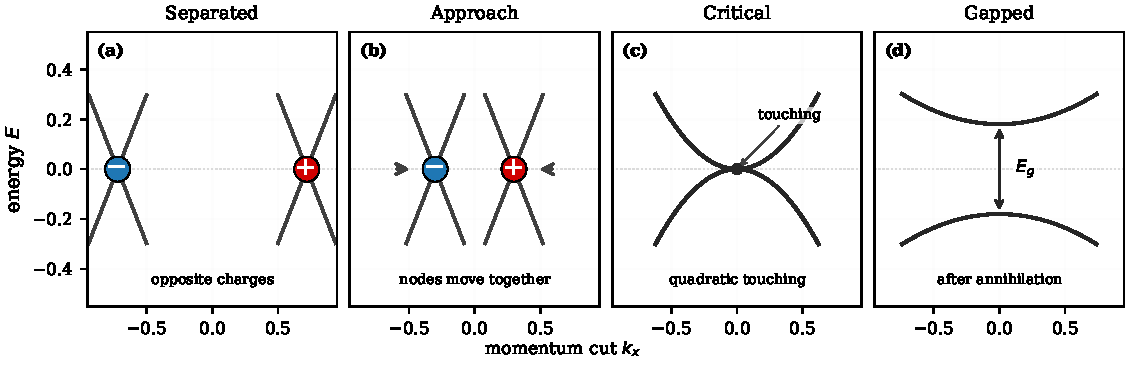
\includegraphics[width=\textwidth]{figures/fig_ch15_weyl_annihilation_step178.pdf}
  \caption{Weyl-point pair annihilation along a one-dimensional momentum cut
  $k_x$.
  (a)~Two separated Weyl nodes of opposite chirality: blue~$(\chi=-1)$,
  red~$(\chi=+1)$, each with a local linear crossing.
  (b)~The nodes approach as a lattice parameter is tuned.
  (c)~At the critical point the charges are coincident and the dispersion
  becomes quadratic along the merging direction; the net monopole charge
  vanishes.
  (d)~Beyond the transition a gap~$E_g$ opens; the resulting phase is
  topologically trivial in the Weyl sense.}
  \label{fig:ch15-weyl-annihilation}
\end{figure}

\subsection{The Nielsen--Ninomiya theorem in 3D}
\label{sec:ch15-nn}

In a compact 3D Brillouin zone (a torus $T^3$), the total monopole
charge must vanish:
\begin{equation}\label{eq:ch15-nn}
  \sum_i \chi_i = 0\,.
\end{equation}

\begin{proof}
The total Berry flux through the boundary of the Brillouin zone is
zero (because the torus has no boundary).  By Gauss's theorem, the
total enclosed charge vanishes.
\end{proof}

This means Weyl points always come in pairs of opposite chirality,
analogous to the pairing of 2D Dirac points (the
fermion-doubling theorem).

\section{Weyl points in photonic crystals}
\label{sec:ch15-photonic}

\subsection{Symmetry requirements}
\label{sec:ch15-symmetry}

A Weyl point requires the breaking of either time-reversal ($\Top$) or
inversion ($\Pop$) symmetry (or both).  The reason is as follows.

If both $\Top$ and $\Pop$ are present, the combined operation
$\Top\Pop$ is an anti-unitary symmetry that maps $\kvec$ to itself
(because $\Top:\kvec\to-\kvec$ and $\Pop:\kvec\to-\kvec$, so
$\Top\Pop:\kvec\to\kvec$).  Since $(\Top\Pop)^2=\Top^2\Pop^2=+1$ for
photons ($\Top^2=+1$, $\Pop^2=+1$), the anti-unitary constraint does
not force Kramers degeneracy.  However, the real-symmetric structure of
the combined eigenproblem typically enforces at least a twofold
degeneracy at every $\kvec$ point, making the minimal band touching a
four-fold Dirac point rather than a two-fold Weyl point.

Breaking either $\Top$ or $\Pop$ removes this constraint and allows
isolated two-fold Weyl points.

\subsection{Classification of photonic Weyl systems}
\label{sec:ch15-classification}

\begin{center}
\begin{tabular}{lccl}
  \toprule
  \textbf{Symmetry broken} & $\Top$ & $\Pop$ &
    \textbf{Example systems} \\
  \midrule
  Inversion only & yes & no &
    Chiral photonic crystals, asymmetric gyroid \\
  Time reversal only & no & yes &
    Gyromagnetic 3D crystals \\
  Both & no & no &
    General magneto-optic + chiral \\
  \bottomrule
\end{tabular}
\end{center}

The case of broken $\Pop$ with preserved $\Top$ is most common in
photonic experiments, because chiral 3D structures can be fabricated
by multi-layer lithography or 3D printing without requiring
magneto-optical materials \cite{lu2012weyl}.

\subsection{The double gyroid photonic crystal}
\label{sec:ch15-gyroid}

One of the first predicted photonic Weyl-point systems is based on the
gyroid minimal surface \cite{ozawa2018topological,liu2021observation}: a triply periodic surface that divides space
into two interpenetrating labyrinthine channels.

In the \emph{single} gyroid structure, the photonic crystal has
body-centred-cubic symmetry with both $\Top$ and $\Pop$.  The band
structure shows Dirac points (four-fold) at high-symmetry points.

In the \emph{double} gyroid, the two channels are filled with different
dielectric materials ($\varepsilon_1\neq\varepsilon_2$), breaking
$\Pop$ while preserving $\Top$.  Each four-fold Dirac point splits into
two Weyl points of opposite chirality, separated in $\kvec$-space by an
amount proportional to the asymmetry $|\varepsilon_1-\varepsilon_2|$.

The positions of the Weyl points in the Brillouin zone are constrained
by the remaining symmetries ($C_3$ rotations along the body diagonal),
which force the Weyl points to lie along high-symmetry lines.

\subsection{Stacked 2D photonic crystals}
\label{sec:ch15-stacked}

A simpler approach creates Weyl points by stacking identical 2D
photonic crystal layers with a controlled interlayer coupling.  If each
2D layer has Dirac points at $K$ and $K'$, the interlayer coupling
disperses these degeneracies along $k_z$, creating either:
\begin{itemize}
  \item A \emph{nodal line}: a continuous ring of degeneracies in
  $(k_x,k_y,k_z)$ space (when $\Top+\Pop$ is preserved)
\cite{kawabata2019symmetry}.
  \item \emph{Weyl points}: isolated degeneracies (when $\Pop$ or
  $\Top$ is broken by the stacking geometry or material choice).
\end{itemize}

The interlayer coupling strength $t_z$ controls the $k_z$-dispersion
and hence the separation of Weyl points.

\section{Surface states and Fermi arcs}
\label{sec:ch15-surface}

\subsection{The surface Brillouin zone}
\label{sec:ch15-surface-bz}

Consider a semi-infinite 3D photonic crystal with a surface perpendicular
to $\hat{x}$.  The surface states are labelled by the surface-parallel
wavevector $\kvec_\parallel=(k_y,k_z)$ and form a 2D band structure
$\omega_{\mathrm{surf}}(\kvec_\parallel)$~\cite{kane2005sub}.

\subsection{Derivation of Fermi arcs from slice Chern numbers}
\label{sec:ch15-arcs-derivation}

The existence of surface states can be understood through the
$k_z$-dependent Chern number $\Chern_n(k_z)$ defined in
\eqref{eq:ch15-slice-chern}.

Consider the 2D slice at a given $k_z$.  If $\Chern_n(k_z)\neq 0$,
the bulk-edge correspondence for 2D systems
(Theorem~\ref{thm:ch8-bec}) predicts $|\Chern_n(k_z)|$ chiral edge modes
at the surface.  These edge modes have a definite group velocity along
$k_y$ and appear at a specific frequency $\omega_{\mathrm{edge}}(k_y,k_z)$.

As $k_z$ sweeps between two Weyl points of opposite chirality at
$k_{z,1}$ and $k_{z,2}$, the Chern number changes from $+1$ to $0$
(or $0$ to $-1$, etc.).  In the region where $\Chern(k_z)=1$, there is
one surface mode; outside this region, there is none.  The surface mode
therefore exists only for $k_z\in(k_{z,1},k_{z,2})$, tracing an
\emph{open arc} in the surface Brillouin zone.

At a fixed frequency equal to the Weyl-point frequency, this arc is
called a \emph{Fermi arc} (by analogy with the electronic case).  The
Fermi arc connects the projections of the two Weyl points onto the
surface Brillouin zone.

\begin{remark}
  The Fermi arcs are \emph{open} curves, not closed loops.  This is
  topologically possible because the arcs terminate at the projected
  Weyl points, where the surface states merge into the bulk continuum.
  Open Fermi arcs have no analog in 2D topological systems, where edge
  modes always form closed dispersion curves crossing the bulk gap.
\end{remark}

Figure~\ref{fig:ch15-weyl-chern-slices} summarises this structure
schematically.

\begin{figure}[t]
  \centering
  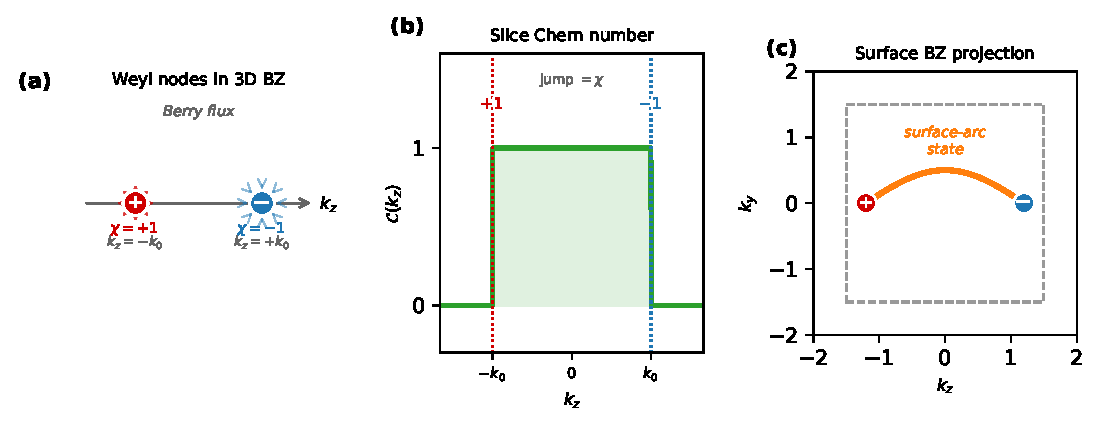
\includegraphics[width=0.95\textwidth]{figures/fig_ch15_weyl_chern_slices_step236.pdf}
  \caption{Weyl points as Berry-curvature monopoles.
  \textbf{(a)}~Two Weyl nodes at $k_z=\pm k_0$ with chiralities
  $\chi=+1$ (source, red) and $\chi=-1$ (sink, blue); Berry-flux
  arrows indicate the monopole and anti-monopole character.
  \textbf{(b)}~The 2D slice Chern number $\Chern(k_z)$ jumps by
  $+\chi$ when the slice passes through a Weyl node, giving the
  step function $0\to 1\to 0$ for the lower band.
  \textbf{(c)}~Surface Brillouin zone showing the photonic
  surface-arc state (orange) connecting the projected Weyl nodes.
  The arc exists only for $k_z$ values where $\Chern(k_z)\neq 0$,
  as required by the bulk--edge correspondence applied slice by
  slice.}
  \label{fig:ch15-weyl-chern-slices}
\end{figure}

\subsection{Fermi-arc connectivity}
\label{sec:ch15-connectivity}

The connectivity of Fermi arcs is topologically constrained: each Weyl
point must be the endpoint of exactly $|\chi|$ arcs.  For charge-1
Weyl points ($|\chi|=1$), each is connected to exactly one other Weyl
point of opposite chirality by a single arc.  The arc cannot terminate
in the interior of the surface Brillouin zone.

When multiple pairs of Weyl points are present, the arcs can connect
them in different patterns, depending on the surface orientation and
termination.  Different surface terminations of the same bulk crystal
can produce different arc connectivity patterns.

\section{Experimental observation of photonic Weyl points}
\label{sec:ch15-experiments}

\subsection{Microwave experiments}
\label{sec:ch15-microwave}

The first experimental observations of photonic Weyl points were achieved
in 3D-printed metallic structures at microwave frequencies
\cite{noh2017experimental,price2022roadmap}.  The
experiments measured:
\begin{itemize}
  \item The bulk band structure, confirming the linear dispersion near
  the Weyl point.
  \item The surface states, showing the characteristic Fermi-arc
  connectivity.
  \item The robustness of the Weyl points to perturbations (they move
  but do not gap).
\end{itemize}

\subsection{Photonic crystal observations}
\label{sec:ch15-photonic-obs}

Weyl points have also been observed in
\cite{ozawa2018topological,noh2017experimental}:
\begin{itemize}
  \item Stacked dielectric photonic crystal slabs with controlled
  interlayer coupling.
  \item Chiral woodpile structures (alternating layers of rods with
  rotation between layers).
  \item Metamaterial waveguide arrays.
\end{itemize}

\section{Nodal lines and higher-order degeneracies}
\label{sec:ch15-nodal}

\subsection{Nodal lines}
\label{sec:ch15-nodal-lines}

A \emph{nodal line} is a closed loop of band degeneracies in
$\kvec$-space.  Unlike Weyl points (which are 0-dimensional), nodal
lines are 1-dimensional objects.  They carry a Berry phase of $\pi$
along any path linking the loop:
\begin{equation}\label{eq:ch15-nodal-berry}
  \gamma = \oint_C\Aberryvec\cdot\dd\kvec = \pi
  \quad\text{for } C \text{ linking the nodal line once.}
\end{equation}
This $\pi$ Berry phase is protected by a mirror or glide symmetry that
forces the eigenstates on the nodal line to be degenerate.

Nodal-line photonic crystals produce ``drumhead'' surface states:
surface states that fill a 2D region in the surface Brillouin zone
bounded by the projection of the nodal line, rather than forming a 1D
arc.

\subsection{Multi-Weyl points}
\label{sec:ch15-multi-weyl}

At high-symmetry points in crystals with $C_n$ ($n\geq 3$) rotational
symmetry, Weyl points can carry higher topological charges $|\chi|>1$.
A \emph{double-Weyl point} ($|\chi|=2$) has quadratic dispersion in
the plane perpendicular to the rotation axis and linear dispersion
along it:
\begin{equation}\label{eq:ch15-double-weyl}
  H = v_\perp(k_+^2\sigma_+ + k_-^2\sigma_-) + v_z\delta k_z\sigma_z\,,
\end{equation}
where $k_\pm=\delta k_x\pm\ii\delta k_y$ and
$\sigma_\pm=(\sigma_x\pm\ii\sigma_y)/2$.

A double-Weyl point sources two units of Berry flux and is the endpoint
of two Fermi arcs.

\subsection{Dirac points in 3D}
\label{sec:ch15-3d-dirac}

When both $\Top$ and $\Pop$ are present, the minimal degeneracy at a
band crossing is a four-fold \emph{Dirac point}: two overlapping Weyl
points of opposite chirality.  Breaking $\Top$ or $\Pop$ splits the
Dirac point into a pair of Weyl points.  The separation between the
Weyl points is controlled by the symmetry-breaking strength.

\section{Connection to Maxwell equations}
\label{sec:ch15-maxwell}

The Weyl-point physics described in this chapter is derived from the
same Maxwell eigenvalue problem $\Maxop(\kvec)\mathbf{u}=\omega\Mmat
\mathbf{u}$ that underlies the entire book.  The 3D extension is
straightforward: $\kvec$ now has three components, the Brillouin zone
is a 3D torus $T^3$, and the Berry curvature is a vector field in
3D $\kvec$-space.

The electromagnetic inner product
$\langle\mathbf{u}|\Mgmat|\mathbf{u}'\rangle$ remains essential for
the correct definition of Berry curvature and topological charges.
Using the wrong inner product would give incorrect monopole charges
and Fermi-arc predictions.

The slice Chern number $\Chern_n(k_z)$ is computed using the same
plaquette formula of \chref{ch:computing-chern}, applied to the
2D slice at fixed $k_z$.  The Wilson-loop method extends naturally:
the Wilson loop at each $(k_y,k_z)$ gives a Zak phase whose winding
in $k_y$ at fixed $k_z$ yields $\Chern_n(k_z)$.

\section{Three-dimensional gapped topological phases}
\label{sec:ch15-3d-gapped}

While Weyl semimetals are gapless---their defining feature is the
point-like band touching---three-dimensional photonic systems can also
host \emph{gapped} topological phases
\cite{yang2026non,armitage2017weyl}.  These are the 3D analogs of
the 2D Chern insulator and the 2D $\mathbb{Z}_2$ topological
insulator: the bulk has a complete frequency gap, and the topology
manifests as robust surface states on every boundary.

\subsection{From 2D to 3D: stacking and strong invariants}
\label{sec:ch15-stacking-gapped}

A simple route to a 3D topological insulator begins with a stack of 2D
topological layers.  If each layer is a 2D Chern insulator with
$\Chern=1$, the stacked system has chiral surface states on every face
perpendicular to the stacking axis.  This ``weak'' topological
insulator inherits its topology from the 2D layers and is vulnerable to
disorder that mixes layers.

A \emph{strong} 3D topological insulator, by contrast, has surface
states on \emph{every} surface orientation, protected by a truly 3D
topological invariant.  In electronic systems, this invariant is the
$\mathbb{Z}_2$ index protected by time-reversal symmetry
(Kane and Mele, 2005; Fu, Kane, and Mele, 2007).  The photonic analog
requires a pseudo-time-reversal symmetry, typically constructed from
bianisotropic coupling between TE-like and TM-like modes.

\subsection{The bianisotropic route to a 3D photonic TI}
\label{sec:ch15-bianisotropic-3d}

The most successful experimental realisation of a 3D photonic
topological insulator was demonstrated by Yang et~al.\
\cite{yang2018realization} using an array of metallic split-ring
resonators (SRRs) embedded in a dielectric host.  The SRRs provide
strong bianisotropic coupling---the magneto-electric cross-terms
$\xit$ and $\zetat$ of the material matrix
(Appendix~\ref{app:material-tensors})---which plays the role of
spin-orbit coupling in the electromagnetic context.

The key design principle is as follows.  Each SRR supports both an
electric resonance (responding to $\Efield$) and a magnetic resonance
(responding to $\Hfield$) at the same frequency, with a cross-coupling
$\xit\neq 0$ that mixes the two.  When the SRRs are arranged on a
3D lattice, the resulting photonic band structure exhibits a complete
bulk bandgap with topologically nontrivial bands below the gap.

The measured bulk bandgap extended from approximately $4.3$ to
$6.0\;\mathrm{GHz}$ (a relative bandwidth exceeding $25\%$), which is
remarkably large compared to earlier 2D photonic topological gaps of a
few percent \cite{ozawa2018topological}.  The large gap makes the
surface states well-resolved and experimentally accessible.

\subsection{Surface Dirac cones}
\label{sec:ch15-surface-dirac}

The hallmark of a 3D gapped topological insulator is a single
\emph{Dirac cone} on each surface---a linearly dispersing surface
state that is topologically protected against backscattering by
disorder or defects.

In the Yang et~al.\ experiment, near-field scanning measurements of
the surface electromagnetic field revealed:
\begin{enumerate}
  \item A surface state with linear (conical) dispersion centred at
  $5.1\;\mathrm{GHz}$, lying within the bulk bandgap.
  \item Robust surface propagation along non-planar surfaces,
  including bends and corners, without backscattering.
  \item A penetration depth of approximately $10\;\mathrm{mm}$ into
  the bulk, consistent with the exponential localisation expected from
  a gapped topological surface state.
\end{enumerate}

The surface Dirac cone should be contrasted with the Fermi arcs of a
Weyl semimetal (\secref{sec:ch15-surface}).  A Fermi arc is an
\emph{open} curve in the surface Brillouin zone, terminating at
projected Weyl points; a surface Dirac cone is a \emph{closed} conical
dispersion centred at a time-reversal-invariant momentum.  The arc
exists because the bulk is gapless (Weyl points); the Dirac cone exists
because the bulk is fully gapped.

\subsection{Comparison of 3D gapped and gapless phases}
\label{sec:ch15-gapped-vs-gapless}

The following table summarises the key differences between 3D gapless
(Weyl) and gapped (topological insulator) phases in photonic crystals.

\begin{center}
\begin{tabular}{lcc}
  \toprule
  & \textbf{3D Weyl semimetal} & \textbf{3D topological insulator} \\
  \midrule
  Bulk gap & none (point nodes) & complete frequency gap \\
  Topological invariant & monopole charge $\chi$ & $\mathbb{Z}_2$ or
    3D Chern numbers \\
  Surface states & open Fermi arcs & closed Dirac cone \\
  Symmetry requirement & break $\Top$ or $\Pop$ & pseudo-$\Top$ from
    bianisotropy \\
  Robustness & nodes move, do not gap & gap persists under all
    symmetry-preserving perturbations \\
  Key photonic experiment & Noh et~al.\ (2017) & Yang et~al.\ (2019) \\
  \bottomrule
\end{tabular}
\end{center}

Both phases are derived from the same 3D Maxwell eigenproblem
$\Maxop(\kvec)\mathbf{u}=\omega\Mmat\mathbf{u}$, but with different
material symmetries: broken $\Pop$ or $\Top$ for Weyl semimetals,
and engineered pseudo-$\Top$ for gapped topological insulators.

\subsection{Towards optical-frequency 3D topological insulators}
\label{sec:ch15-optical-3dti}

The Yang et~al.\ demonstration operated at microwave frequencies, where
SRR fabrication is straightforward.  Extending 3D photonic topological
insulators to optical frequencies is an active research frontier
\cite{price2022roadmap}.  The challenges include fabricating 3D
nanostructures with precise bianisotropic response and maintaining a
sufficiently large bandgap relative to fabrication imperfections.  Recent
proposals based on all-dielectric metacrystals and chiral woodpile
structures suggest that optical-frequency 3D topological gaps may be
achievable with current nanofabrication technology \cite{khanikaev2016three}.

\section{Type-I and type-II Weyl points}
\label{sec:ch15-types}

Weyl points come in two types, distinguished by their isofrequency
surfaces \cite{chen2021ideal}.  A type-I Weyl point has a point-like Fermi surface at the
Weyl frequency: the isofrequency contour shrinks to a single point,
with the dispersion forming an upright cone
$\omega=\omega_W\pm v|\delta\kvec|$.

A type-II Weyl point has a tilted cone, so that the isofrequency
surface at $\omega=\omega_W$ is not a point but a pair of electron-
and hole-like pockets touching at the Weyl point.  The effective
Hamiltonian is
$H=v_t k_z\sigma_0 + v(k_x\sigma_x+k_y\sigma_y+k_z\sigma_z)$,
where $v_t>v$ is the tilt velocity.  The tilt breaks Lorentz
invariance but does not change the topological charge of the Weyl
point \cite{noh2017experimental,ozawa2018topological}.

Type-II Weyl points were first observed in photonics by Noh et~al.\
(2017) using a laser-written waveguide array.  The waveguides were
arranged in a face-centred geometry with controlled interlayer
coupling, producing tilted Weyl cones in the propagation-constant
spectrum.  The type-II nature was confirmed by observing the
characteristic ``bowtie'' isofrequency contour using Fourier-space
imaging \cite{noh2017experimental}.

\section{Nodal lines and drumhead surface states}
\label{sec:ch15-nodal-lines-drumhead}

When two bands cross along a line in the 3D Brillouin zone rather
than at an isolated point, the crossing is called a \emph{nodal line}.
Nodal lines can be stabilised by crystal symmetries (e.g.\ mirror or
glide symmetries) and carry a $\pi$ Berry phase around any loop
encircling the line, analogous to the $\pi$ Berry phase at a 2D Dirac
point \cite{kim2015dirac,ozawa2018topological}.

The bulk-boundary correspondence for nodal lines predicts
\emph{drumhead surface states}: flat or nearly flat bands that fill
the interior of the projected nodal line on the surface Brillouin
zone.  These states have a high density of states and are of interest
for enhanced light--matter interaction.

Nodal-line photonic crystals have been realised using dielectric
structures with carefully designed symmetries.  The drumhead states
have been observed as bright, nearly dispersionless features in
angle-resolved transmission measurements
\cite{price2022roadmap}.

\section{Experimental platforms for 3D photonic topology}
\label{sec:ch15-3d-platforms}

Three-dimensional photonic topological phases have been demonstrated
on several platforms:

Laser-written waveguide arrays in fused silica provide type-II Weyl
points and Fermi-arc surface states at optical wavelengths
($\lambda=633\;\mathrm{nm}$).  The paraxial propagation approximation
maps the 3D waveguide structure onto a (2+1)D tight-binding model
with the propagation direction playing the role of time
\cite{noh2017experimental,rechtsman2013photonica}.

Metallic photonic crystals with gyroid or diamond symmetry can
support complete 3D band gaps with nontrivial topology.  The
Weyl points appear as pairs of opposite-charge monopoles in the
3D Brillouin zone, connected by surface Fermi arcs on any
termination \cite{ozawa2018topological}.

Bianisotropic metamaterials (split-ring resonator arrays) realise
3D topological insulators with surface Dirac cones, as discussed in
Chapter~\ref{ch:microwave-crystal}
\cite{yang2018realization,price2022roadmap}.

\section{Surface Dirac cones and topological surface states}
\label{sec:ch15-surface-dirac-cone}

A 3D photonic topological insulator---a material with a nontrivial
$\mathbb{Z}_2$ invariant---supports gapless surface states that form
a Dirac cone in the surface Brillouin zone.  These surface Dirac
cones are the 3D analog of the chiral edge modes of a 2D Chern
insulator: they are topologically protected and cannot be gapped by
any surface perturbation that preserves time-reversal symmetry.

The surface Dirac cone was first observed experimentally by Yang
et~al.\ (2019) in a bianisotropic metamaterial of double split-ring
resonators arranged in a body-centred cubic lattice.  Angle-resolved
transmission measurements on a cleaved crystal surface revealed a
linear dispersion cone at $\bar{\Gamma}$ in the surface Brillouin zone,
with the Dirac frequency at $5.1\;\mathrm{GHz}$ inside the bulk gap
from 4.3 to $6.0\;\mathrm{GHz}$
\cite{yang2018realization,ozawa2018topological}.

The robustness of the surface Dirac cone was confirmed by introducing
surface disorder (randomly removing $10\%$ of the surface resonators)
and observing that the Dirac cone remained intact, with only a slight
broadening of the surface states.  This is consistent with the
$\mathbb{Z}_2$ protection: the surface Dirac cone can be shifted in
energy or broadened by disorder, but it cannot be gapped
\cite{price2022roadmap}.

\subsection{Comparison table: 2D edge modes versus 3D surface states}
\label{sec:ch15-comparison-2d-3d}

The 2D and 3D cases share the same topological origin but differ in
dimensionality and symmetry:
\begin{center}
\begin{tabular}{lll}
  \toprule
  Property & 2D Chern insulator & 3D topological insulator \\
  \midrule
  Bulk invariant & Chern number $\Chern\in\mathbb{Z}$ &
    $\mathbb{Z}_2$ index $\nu\in\{0,1\}$ \\
  Boundary states & chiral edge modes & surface Dirac cone \\
  Protection & against all gap-preserving & against $\Top$-preserving \\
  & perturbations & perturbations \\
  Requires $\Top$ breaking & yes & no \\
  Min.\ boundary modes & $|\Chern|$ & 1 Dirac cone \\
  \bottomrule
\end{tabular}
\end{center}

\section{Photonic Weyl semimetal experiments}
\label{sec:ch15-weyl-experiments}

The theoretical prediction of Weyl points in photonic crystals was
confirmed experimentally in several landmark experiments that
directly observed the key signatures: bulk conical dispersions,
surface Fermi arcs, and robustness against perturbations.

\subsection{The double-gyroid photonic crystal}
\label{sec:ch15-double-gyroid}

The first experimental observation of photonic Weyl points was
reported by Lu et~al.\ (2015) in a double-gyroid photonic crystal
at microwave frequencies \cite{price2022roadmap}.  The double
gyroid is a bicontinuous structure with body-centred cubic symmetry
described by the level-set equation
\begin{equation}\label{eq:ch15-gyroid-level-set}
  f(\rvec) = \sin(2\pi x/a)\cos(2\pi y/a)
  + \sin(2\pi y/a)\cos(2\pi z/a)
  + \sin(2\pi z/a)\cos(2\pi x/a)\,,
\end{equation}
where the two gyroid networks occupy the regions $f>t_0$ and
$f<-t_0$ for a threshold $t_0$.  The structure was fabricated by
3D-printing metallic scaffolds with lattice constant $a=13\;\mathrm{mm}$,
operating in the 5--8~GHz range.

By breaking either time-reversal or inversion symmetry (achieved by
coating one of the two gyroid networks with a metallic layer to
destroy inversion), the authors lifted a four-fold line degeneracy
into pairs of Weyl points with opposite chirality.  Angle-resolved
microwave transmission measurements mapped the bulk band structure
and confirmed the linear conical dispersion near the Weyl frequencies
\cite{ozawa2018topological}.

\subsection{Surface Fermi arcs}
\label{sec:ch15-fermi-arcs-exp}

The surface Fermi arc is the defining experimental signature of a
Weyl semimetal: it is an open contour of constant-frequency surface
states that connects the projections of two Weyl points of opposite
chirality onto the surface Brillouin zone.

The existence of Fermi arcs follows from a topological argument.
Consider a closed loop $\mathcal{C}$ in the surface Brillouin zone
that encircles the projection of a single Weyl point.  The Chern
number of the occupied bands evaluated on $\mathcal{C}$ is
$\Chern(\mathcal{C})=\pm 1$, implying that at least one surface
band must cross the Weyl-point frequency within $\mathcal{C}$.
Since the surface band cannot form a closed contour (it would then
encircle equal numbers of positive and negative chirality
projections and carry zero Chern flux), it must terminate at the
Weyl-point projections.  The resulting open arc is the Fermi arc.

In the double-gyroid experiment, surface Fermi arcs were observed by
measuring the near-field intensity distribution on a cleaved crystal
surface.  The arc-like surface dispersion was clearly visible in the
angle-resolved transmission, connecting pairs of projected Weyl
points as predicted by the bulk-boundary correspondence
\cite{ozawa2018topological,price2022roadmap}.

\subsection{Type-II Weyl points in photonic systems}
\label{sec:ch15-type-ii-exp}

Type-II Weyl points, introduced in \secref{sec:ch15-types}, are
characterised by a strongly tilted cone that intersects the
constant-frequency surface to form electron and hole pockets.  In a
photonic crystal, the ``pockets'' are regions of propagating bulk
modes that coexist with the Weyl frequency, leading to qualitatively
different surface-state physics: the Fermi arcs connect not only the
Weyl-point projections but also merge with the bulk pocket
projections \cite{ozawa2018topological}.

Noh et~al.\ (2017) reported the first observation of type-II Weyl
points in a photonic system using a stacked bilayer photonic crystal
\cite{noh2017experimental}.  The structure consisted of alternating
layers of hexagonal photonic crystal slabs with different in-plane
geometries, creating a three-dimensional photonic crystal with
broken inversion symmetry.  The strongly tilted conical dispersion
was confirmed by angle-resolved reflection measurements, and the
characteristic electron--hole pocket structure was observed at
frequencies near the Weyl point.

\subsection{Ideal Weyl points and minimal photonic designs}
\label{sec:ch15-ideal-weyl}

An ``ideal'' Weyl semimetal has its Weyl points located exactly at the
Fermi level (or, in the photonic case, at a frequency isolated from
all other bands), so that the only states at that frequency are the
Weyl cones and the surface arcs.  This ideal condition maximises the
length of the Fermi arcs and the surface-state density of states.

Yang et~al.\ (2018) realised an ideal Weyl system using a
saddle-shaped metallic inclusion in a body-centred cubic unit cell
\cite{yang2018realization,yang2017discovery}.  The design produced Weyl points that
were separated from all other bands by a complete frequency gap,
giving the longest possible Fermi arcs spanning the entire surface
Brillouin zone.  The experiment was performed at microwave
frequencies with 3D-printed metallic structures, and the surface arcs
were mapped by near-field scanning measurements.

\begin{figure}[t]
  \centering
  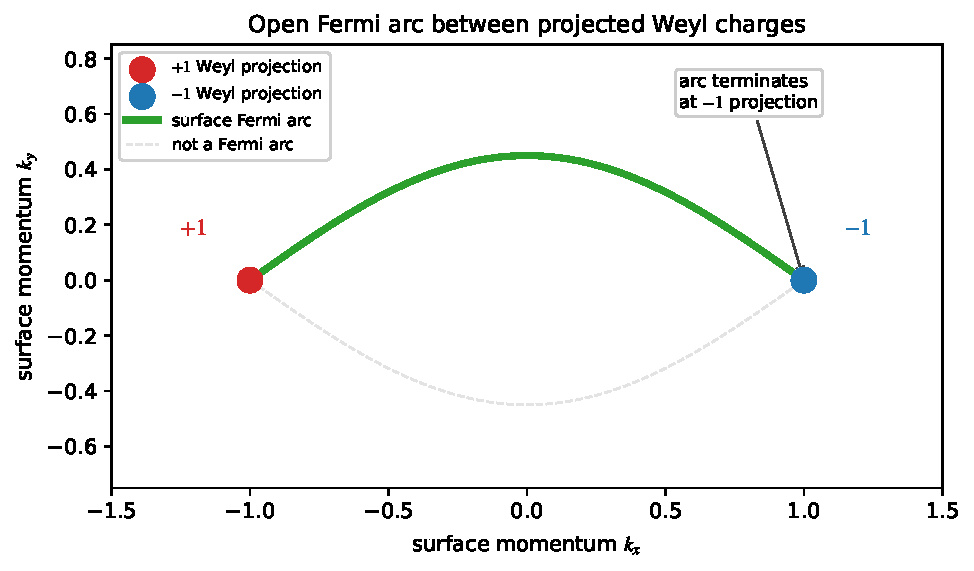
\includegraphics[width=0.78\textwidth]{figures/fig_ch15_weyl_fermi_arc.pdf}
  \caption{A surface Fermi arc connects projected Weyl charges of opposite
  chirality.  Unlike an ordinary constant-frequency contour, the arc is open:
  it terminates on the surface projections of bulk Weyl points, expressing
  the Chern-number jump across the Weyl node.}
  \label{fig:ch15-weyl-fermi-arc}
\end{figure}

\section*{Exercises}

\begin{exercise}
  Compute the Berry curvature of the lower band of the isotropic Weyl
  Hamiltonian $H=v(\delta k_x\sigma_x+\delta k_y\sigma_y
  +\delta k_z\sigma_z)$ and verify that it has the monopole form
  \eqref{eq:ch15-general-berry} with $\chi=+1$.
\end{exercise}

\begin{exercise}
  Show that no $2\times 2$ Hermitian perturbation can gap the 3D Weyl
  Hamiltonian \eqref{eq:ch15-weyl-hamiltonian}.  \emph{Hint:} write the
  most general $2\times 2$ Hermitian matrix $\delta H=\sum_a\delta d_a
  \sigma_a+\delta d_0\mathbf{I}$ and show that adding it to $H_W$ only
  shifts the Weyl point.
\end{exercise}

\begin{exercise}
  For a pair of Weyl points at $\kvec_\pm=(0,0,\pm k_0)$ with
  chiralities $\chi_\pm=\pm 1$, compute the slice Chern number
  $\Chern(k_z)$ for $|k_z|<k_0$, $|k_z|>k_0$, and $k_z=\pm k_0$.
  Use this to derive the existence and extent of the Fermi arc on the
  $(001)$ surface.
\end{exercise}

\begin{exercise}
  Explain why Weyl points require the breaking of either $\Top$ or
  $\Pop$ (or both).  \emph{Hint:} show that $\Top\Pop$ symmetry forces
  the eigenstates to be at least doubly degenerate at every $\kvec$ in
  a system where both are preserved.
\end{exercise}

\begin{exercise}
  A photonic nodal line in a 3D crystal is a closed loop in
  $\kvec$-space where two bands are degenerate.  Show that the Berry
  phase $\gamma=\oint_C\Aberryvec\cdot\dd\kvec$ for a path $C$ linking
  the nodal line once is quantised to $\pi$.  What symmetry protects
  this quantisation?
\end{exercise}

\begin{exercise}
  For a double-Weyl point with Hamiltonian \eqref{eq:ch15-double-weyl},
  compute the Berry flux through a sphere enclosing the degeneracy and
  verify that the topological charge is $|\chi|=2$.
\end{exercise}

\begin{exercise}
  Consider a 3D photonic crystal with a single pair of Weyl points on
  the $k_z$ axis.  If the crystal is truncated to form a slab of
  thickness $L$ in the $x$-direction, describe qualitatively how the
  Fermi arcs on the top and bottom surfaces connect through the slab
  as $L$ decreases.
\end{exercise}


\chapter{Synthetic Dimensions}
\label{ch:synthetic-dimensions}
% ======================================================================
%  Chapter 16 — Synthetic Dimensions  (DEEPLY EXPANDED)
%  photonic systems, including Harper-Hofstadter, 4D QHE, experiments
\cite{kane2005sub}.
% ======================================================================

\section{Beyond physical dimensions}
\label{sec:ch16-intro}

The topological phenomena explored in Chapters~7--15 occur in systems
with two or three spatial dimensions.  But topology is not limited by
the number of physical dimensions: it depends on the structure of the
Hilbert space and the connectivity of the parameter manifold, not on the
spatial geometry of the laboratory.

A \emph{synthetic dimension} is an internal degree of freedom---such as
the frequency, orbital angular momentum, spin, or mode index of a
photon---that is reinterpreted as an extra spatial coordinate through
engineered couplings.  By coupling modes along the synthetic axis with
controlled phases, one can create effective lattice models in dimensions
higher than the physical space \cite{lin2018constructing}.  This opens a route to observing
topological phases that have no direct analog in lower-dimensional
systems, most notably the four-dimensional quantum Hall effect.

This chapter derives the synthetic-dimension framework from Maxwell's
equations \cite{ozawa2018topological,liu2021observation}, explains how the Harper--Hofstadter model and higher-dimensional
Chern insulators can be implemented in photonic systems, and surveys the
principal experimental platforms \cite{kim2020recent}.

\section{Frequency as a synthetic dimension}
\label{sec:ch16-frequency}

\subsection{The coupled-mode picture}
\label{sec:ch16-coupled-mode}

Consider a ring resonator supporting a comb of equally spaced resonant
frequencies $\omega_m=\omega_0+m\Omega_{\mathrm{FSR}}$
($m=0,\pm 1,\pm 2,\ldots$), where $\Omega_{\mathrm{FSR}}=2\pi c/(n_g L)$
is the free spectral range, $n_g$ is the group index, and $L$ is the
round-trip length
\cite{press2026photonic}.  In the absence of modulation, the modes are
decoupled and the frequency index $m$ labels a one-dimensional lattice
with lattice constant $\Omega_{\mathrm{FSR}}$.

Now apply an electro-optic phase modulation at frequency
$\Omega_{\mathrm{mod}}=\Omega_{\mathrm{FSR}}$ to the resonator.  The
modulation creates a time-dependent coupling between adjacent frequency
modes.  In the slowly varying envelope approximation, the amplitude
$a_m(t)$ of mode $m$ satisfies the coupled-mode equation
\begin{equation}\label{eq:ch16-coupled-mode}
  \ii\pderiv{a_m}{t}
  = \omega_m\,a_m + \kappa\bigl(\ee^{\ii\phi}\,a_{m-1}
  + \ee^{-\ii\phi}\,a_{m+1}\bigr)\,,
\end{equation}
where $\kappa$ is the modulation strength and $\phi$ is the modulation
phase.  This is mathematically identical to the tight-binding equation
for a particle hopping on a 1D lattice with nearest-neighbour coupling
$\kappa\ee^{\pm\ii\phi}$.

The frequency axis has thus become a \emph{synthetic spatial dimension}:
hopping along the frequency ladder is controlled by the electro-optic
modulation, and the hopping phase $\phi$ plays the role of a Peierls
phase (synthetic gauge field)
\cite{raghu2008analogs}.

\begin{figure}[t]
  \centering
  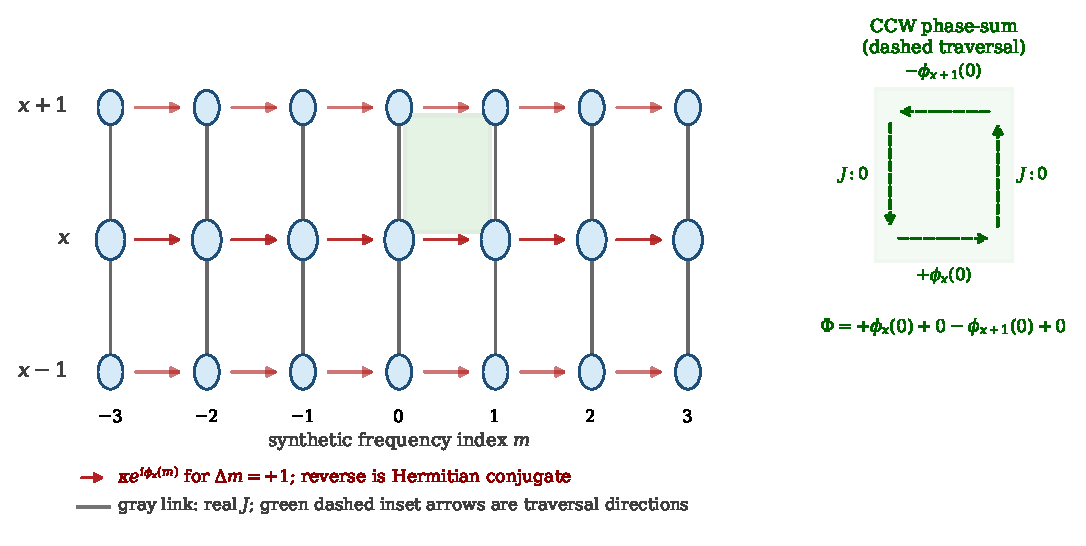
\includegraphics[width=0.88\textwidth]{figures/fig_synthetic_frequency_ladder.pdf}
  \caption{Synthetic frequency dimension in a modulated resonator
    array.  Each column represents a frequency mode
    $\omega_m=\omega_0+m\Omega$; each row represents a physical
    resonator at real-space site $x$.  Red rightward arrows denote
    the Peierls hopping $\kappa\ee^{\ii\phi_x(m)}$ along the
    synthetic frequency direction ($\Delta m=+1$); the reverse
    ($\Delta m=-1$) hopping is the Hermitian conjugate \cite{yuan2018synthetic,yuan2015photonic}.  Gray
    vertical links represent the real-valued inter-site coupling $J$.
    The green shaded plaquette between columns $m=0$ and $m=1$ at
    sites $x$ and $x{+}1$ carries a gauge-invariant flux
    $\Phi=\phi_x(0)-\phi_{x+1}(0)$, computed by summing the
    directed link phases counter-clockwise.  In the inset this is
    displayed as $+\phi_x(0)+0-\phi_{x+1}(0)+0$: the two vertical
    $J$ links contribute zero phase.  In the inset, the dashed green
    arrows show the traversal directions used for this phase sum,
    whereas the red arrows in the main lattice show the physical
    hopping direction $\Delta m=+1$.  This flux is the
    synthetic-dimension analog of an applied magnetic field.}
  \label{fig:ch16-synthetic-ladder}
\end{figure}

\subsection{Derivation from Maxwell's equations}
\label{sec:ch16-maxwell-derivation}

To maintain the Maxwell-first spirit of this book, we derive the
coupled-mode equation \eqref{eq:ch16-coupled-mode} from the
time-dependent Maxwell equations with a modulated material matrix.

Consider a ring resonator whose permittivity is modulated:
\begin{equation}\label{eq:ch16-eps-modulated}
  \varepsilon(t) = \bar\varepsilon\bigl[1 + 2\eta\cos(\Omega_{\mathrm{mod}}t-\phi)\bigr] \,.
\end{equation}
Here $\eta\ll 1$ is the modulation depth.  The minus sign in
\eqref{eq:ch16-eps-modulated} is a convention: with fields written as
$\ee^{-\ii\omega t}$, it makes $\phi$ the Peierls phase for the
rightward frequency transition $m\to m+1$.  If the physical drive is
instead written as $\cos(\Omega_{\mathrm{mod}}t+\theta)$, then the
Peierls phase used below is $\phi=-\theta$.  The electric field in the
resonator is expanded in the unperturbed mode basis:
$E(t)=\sum_m a_m(t)\,\mathcal E_m\,\ee^{-\ii\omega_m t}$, where
$\mathcal E_m$ is the mode profile of mode $m$.

Substituting into the Maxwell wave equation and using the rotating-wave
approximation (retaining only the slowly varying terms), one obtains
\begin{equation}\label{eq:ch16-rwa}
  \ii\dot{a}_m = \kappa_{\mathrm{eff}}\bigl(\ee^{\ii\phi}\,a_{m-1}
  + \ee^{-\ii\phi}\,a_{m+1}\bigr)\,,
\end{equation}
The phase factors in \eqref{eq:ch16-rwa} follow directly from the
time convention just fixed: the coupling from $m-1$ to $m$ uses the
$\ee^{-\ii\Omega_{\mathrm{mod}}t+\ii\phi}$ component of the modulation,
whereas the coupling from $m+1$ to $m$ uses the complex-conjugate
component.  Thus the rightward hopping carries $+\phi$ and the reverse
hopping carries $-\phi$, matching \figref{fig:ch16-synthetic-ladder}.
The effective coupling is
\begin{equation}\label{eq:ch16-coupling}
  \kappa_{\mathrm{eff}} = \frac{\eta\omega_0}{2}
  \frac{\int|\mathcal E_m|^2\varepsilon_0\,\dd V}
  {\int|\mathcal E_m|^2\bar\varepsilon\,\dd V}
  \approx \frac{\eta\omega_0}{2}\,.
\end{equation}
This confirms that the coupled-mode equation
\eqref{eq:ch16-coupled-mode} is a direct consequence of the Maxwell
equations with a time-modulated permittivity.

\section{The Harper--Hofstadter model from synthetic dimensions}
\label{sec:ch16-harper}

\subsection{Adding a physical dimension}
\label{sec:ch16-2d-lattice}

To create a 2D lattice, we combine the synthetic frequency dimension
with one physical spatial dimension.  Consider an array of $N$ coupled
ring resonators, each supporting a frequency comb and each individually
modulated.  The physical coupling between adjacent rings provides
hopping along the spatial direction $x$, and the intra-ring modulation
provides hopping along the synthetic frequency direction $m$.

The amplitude $a_{m,x}(t)$ of mode $m$ in ring $x$ satisfies
\begin{equation}\label{eq:ch16-2d-hamiltonian}
  \ii\dot{a}_{m,x}
  = J\bigl(a_{m,x-1}+a_{m,x+1}\bigr)
  + \kappa\bigl(\ee^{\ii\phi_x}a_{m-1,x}+\ee^{-\ii\phi_x}a_{m+1,x}\bigr)\,,
\end{equation}
where $J$ is the inter-ring coupling and $\phi_x=\phi_0+\alpha x$ is
the modulation phase that varies linearly along the array.

\subsection{Mapping to the Hofstadter Hamiltonian}
\label{sec:ch16-hofstadter}

In the Bloch-wave ansatz $a_{m,x}=\ee^{\ii(k_x x + k_m m)}b_{m,x}$,
the equation of motion \eqref{eq:ch16-2d-hamiltonian} becomes
\cite{ozawa2018topological}
\begin{equation}\label{eq:ch16-hofstadter}
  \boxed{%
  E\,b_{m,x} = 2J\cos(k_x)\,b_{m,x}
  + 2\kappa\cos(k_m+\alpha x+\phi_0)\,b_{m,x}\,,}
\end{equation}
which is the \emph{Harper equation}, the eigenvalue equation of the
Hofstadter model with flux $\alpha$ per plaquette.  When
$\alpha/(2\pi)=p/q$ is a rational number, the spectrum splits into $q$
subbands, forming the famous Hofstadter butterfly.

The key insight is that the synthetic gauge flux $\alpha$ is fully
controllable through the modulation phase gradient.  By choosing
$\alpha=2\pi p/q$ for small $q$, one can access topological regimes
(nonzero Chern numbers) with experimentally reasonable modulation
parameters.

\subsection{Topological bands and edge states}
\label{sec:ch16-harper-topology}

Each subband of the Harper equation carries a Chern number determined by
the Diophantine equation $\Chern_r = \sigma_r$, where $\sigma_r$ is
the quantised Hall conductance of the $r$-th gap.  For
$\alpha/(2\pi)=1/3$ (three subbands), the Chern numbers are
$\Chern_1=+1$, $\Chern_2=-2$, $\Chern_3=+1$.

In the synthetic-dimension realisation, the ``edge'' of the frequency
lattice is set by the finite bandwidth of the modulation or the gain
medium.  Edge states appear at the boundary of the synthetic lattice
and propagate unidirectionally along the physical direction, directly
analogous to quantum Hall edge states.

\section{Four-dimensional quantum Hall effect}
\label{sec:ch16-4d}

\subsection{Topology in four dimensions}
\label{sec:ch16-4d-topology}

In four spatial dimensions, the quantum Hall effect is characterised by
the \emph{second Chern number}, a topological invariant defined on the
4D Brillouin zone $T^4$:
\begin{equation}\label{eq:ch16-second-chern}
  \Chern_2 = \frac{1}{8\pi^2}\int_{T^4}
  \Tr(\mathcal{F}\wedge\mathcal{F})\,,
\end{equation}
where $\mathcal{F}$ is the non-Abelian Berry curvature 2-form of the
occupied bands (Appendix~B).  The 4D quantum Hall effect predicts a
\emph{nonlinear} Hall response: a current perpendicular to three
applied fields, with a quantised coefficient proportional to $\Chern_2$.

The second Chern number is fundamentally different from the first Chern
number: it requires at least four dimensions to be nonzero and detects
topological features (``instanton-like'' structures in the Berry
connection) that have no analog in lower dimensions.

\subsection{Synthetic 4D lattice}
\label{sec:ch16-4d-lattice}

To realise a 4D topological system in a photonic experiment, one
combines two physical dimensions with two synthetic dimensions.  For
example, a 2D array of ring resonators, each modulated at two
frequencies $\Omega_1$ and $\Omega_2$, creates a 4D lattice with
coordinates $(x,y,m_1,m_2)$, where $x,y$ are physical positions and
$m_1,m_2$ are frequency-mode indices along the two synthetic axes.

The effective 4D Hamiltonian can be engineered to have nonzero $\Chern_2$
by choosing the modulation phases to create a non-trivial Berry
connection on the 4D Brillouin zone.

\subsection{Experimental signatures}
\label{sec:ch16-4d-signatures}

The second Chern number manifests as a quantised nonlinear response
\cite{ozawa2018topological,price2022roadmap}.
In a photonic 4D system, this appears as a pump-induced spectral flow:
when the modulation phase is adiabatically varied (implementing a
``magnetic field'' in one of the synthetic planes), photons are pumped
across bands in a direction perpendicular to the applied field and to
the synthetic dimension, with a rate quantised by $\Chern_2$.

This effect was experimentally observed in a 2D photonic waveguide
array with two synthetic dimensions implemented by adiabatic variation
of coupling parameters along the propagation axis.  The measured
spectral flow matched the theoretical prediction $\Chern_2=1$ for the
engineered lattice model.

\section{Other synthetic-dimension platforms}
\label{sec:ch16-platforms}

\subsection{Orbital angular momentum}
\label{sec:ch16-oam}

The orbital angular momentum (OAM) of light provides a natural
synthetic dimension.  Modes of a ring resonator or a multimode fibre
carry a discrete OAM quantum number $\ell=0,\pm 1,\pm 2,\ldots$.
Coupling between adjacent OAM modes can be induced by inserting an
astigmatic element (such as a tilted mirror or a spatial light
modulator) that mixes modes with $\Delta\ell=\pm 1$.

The coupling phase can be controlled by the orientation of the
astigmatic element, providing a synthetic gauge field along the OAM
axis.  Combined with a physical spatial dimension, this creates a 2D
lattice with controllable magnetic flux.

\subsection{Temporal modes and time multiplexing}
\label{sec:ch16-temporal}

In a fibre loop, successive round-trip pulses form a 1D lattice in
``time'' (the discrete time step labelled by the round-trip number).
Coupling between pulses is provided by a beam splitter or a variable
coupler, and the coupling phase can be controlled electronically.

By combining the time-multiplexed lattice with a spatial array of
fibre loops, one can create 2D and higher-dimensional effective
lattices.  This approach has been used to demonstrate the
Hofstadter butterfly, anomalous Floquet topological phases, and
Anderson localisation in synthetic lattices \cite{guglielmon2017photonic}.

\subsection{Spin and polarisation}
\label{sec:ch16-spin}

The polarisation state of light (left/right circular, or
horizontal/vertical) provides a two-site synthetic dimension.  While
this is too short to form a lattice by itself, it can serve as the
``sublattice'' degree of freedom in models such as the SSH chain or the
Haldane model, with the spatial lattice providing the remaining
dimension.

\section{Quantitative analysis of synthetic-dimension experiments}
\label{sec:ch16-quantitative}

To appreciate both the power and the limitations of synthetic
dimensions, it is instructive to work through the key numbers for the
two principal experimental platforms.

\subsection{Ring-resonator frequency lattice}
\label{sec:ch16-ring-numbers}

Consider a silicon nitride microring resonator with group index
$n_g=2.0$ and circumference $L=2\pi R=628\;\mu\mathrm{m}$
($R=100\;\mu\mathrm{m}$)
\cite{initio2026pdf}.  The free spectral range is
\begin{equation}\label{eq:ch16-fsr-numerical}
  \Omega_{\mathrm{FSR}} = \frac{2\pi c}{n_g L}
  \approx 2\pi\times 150\;\mathrm{GHz}\,,
\end{equation}
so the frequency modes are spaced by $150\;\mathrm{GHz}$ in the
C-band around $\lambda=1550\;\mathrm{nm}$.

With electro-optic modulation depth $\eta=0.01$ and carrier frequency
$\omega_0/(2\pi)=193\;\mathrm{THz}$, the effective hopping from
\eqref{eq:ch16-coupling} is
\begin{equation}\label{eq:ch16-kappa-numerical}
  \kappa_{\mathrm{eff}} \approx \frac{\eta\omega_0}{2}
  \approx 2\pi\times 0.97\;\mathrm{THz}\,.
\end{equation}
The ratio $\kappa_{\mathrm{eff}}/\Omega_{\mathrm{FSR}}\approx 6.5$
is much larger than unity, which \emph{violates} the tight-binding
assumption underlying \eqref{eq:ch16-coupled-mode}: the modulation
couples not only nearest-neighbour frequency modes but also
next-nearest and more distant modes.  To restore the tight-binding
regime, one must reduce $\eta$ to $\sim 10^{-4}$ or use a longer
resonator with smaller FSR.

This quantitative tension between coupling strength and tight-binding
validity is a central design challenge for synthetic-dimension
experiments \cite{ozawa2018topological,price2022roadmap}.

\subsection{Waveguide-array Floquet lattice}
\label{sec:ch16-waveguide-numbers}

The Rechtsman helical-waveguide experiment (\chref{ch:floquet})
can also be viewed as a synthetic-dimension platform, where the
propagation coordinate $z$ is the synthetic time axis.  The key
parameters are: helix radius $R_h=8\;\mu\mathrm{m}$, pitch
$\Lambda=1\;\mathrm{cm}$, inter-waveguide spacing
$d=22\;\mu\mathrm{m}$, and operating wavelength
$\lambda=633\;\mathrm{nm}$ in borosilicate glass ($n_0=1.46$)
\cite{rechtsman2013photonica}.

The effective modulation frequency is
$\Omega_{\mathrm{mod}}=2\pi/\Lambda\approx 628\;\mathrm{m}^{-1}$,
and the inter-waveguide coupling is
$J\approx 1.0\;\mathrm{cm}^{-1}$.  The effective gauge flux per
plaquette is $\Phi\approx k_0 R_h^2(2\pi/\Lambda)^2 a/(2\pi)$,
where $k_0=2\pi n_0/\lambda$ and $a=d\sqrt{3}/2$ is the lattice
constant.  For the experimental parameters,
$\Phi\approx 0.21\times 2\pi$, which places the system in a
topological regime with Chern number $\Chern=\pm 1$.

The topological gap width is approximately
$\Delta J\sim J\sin(\pi\Phi/\Phi_0)\approx 0.6\;\mathrm{cm}^{-1}$,
corresponding to a localisation length of
$\ell_{\mathrm{edge}}\sim v_g/\Delta J\approx 17\;\mu\mathrm{m}$
for the edge mode.  The sample length of $10\;\mathrm{cm}$ then
corresponds to $\sim 10$ modulation periods and $\sim 600$
localisation lengths, so the topological protection is well developed.

\section{Limitations and outlook}
\label{sec:ch16-limitations}

Synthetic dimensions offer remarkable flexibility in engineering
effective Hamiltonians \cite{price2022roadmap}, but they come with
important limitations.

The synthetic lattice is typically \emph{finite}: the frequency comb of
a ring resonator has a finite bandwidth set by the gain or loss
spectrum, and the OAM modes are limited by the aperture of the optical
elements.  This finiteness truncates the synthetic dimension and creates
hard boundaries, which can host edge states but also introduce
finite-size effects that complicate the interpretation of topological
signatures.

Interactions between photons in synthetic-dimension systems are
generally absent, because the photon-photon interaction is negligible in
most optical media.  This limits the exploration of strongly correlated
topological phases (such as fractional quantum Hall states) in
synthetic-dimension photonic systems.

Looking forward, the combination of synthetic dimensions with
nonlinear or quantum photonic platforms (Chapter~\ref{ch:nonlinear-quantum})
may overcome these limitations, enabling the study of interacting
topological phases in dimensions and geometries that are inaccessible
in condensed matter.

\section{Experimental platforms for synthetic dimensions}
\label{sec:ch16-platforms-experimental}

Several photonic platforms have been used to realise synthetic
dimensions, each offering different trade-offs between tunability,
dimensionality, and loss.

\subsection{Ring resonators with frequency modes}
\label{sec:ch16-ring-freq}

A single optical ring resonator supports a comb of equally spaced
frequency modes separated by the free spectral range
$\mathrm{FSR}=c/(n_{\mathrm{eff}}L)$, where $L$ is the round-trip
length.  These modes form a natural 1D lattice in frequency space.
An electro-optic modulator driven at $\Omega=\mathrm{FSR}$ creates
nearest-neighbour coupling between adjacent frequency modes with a
controllable complex phase, providing the Peierls hopping
\eqref{eq:ch16-coupling} \cite{ozawa2018topological,price2022roadmap}.

For a typical silicon ring with $L=2\pi\times 50\;\mu\mathrm{m}$ and
$n_{\mathrm{eff}}=2.4$, the FSR is $\approx 400\;\mathrm{GHz}$.
With a modulation depth of $V_m/V_\pi\approx 0.3$, the effective
hopping is $\kappa_{\mathrm{eff}}\approx 0.3\times\mathrm{FSR}
\approx 120\;\mathrm{GHz}$, which is sufficient to observe topological
edge states spanning several frequency modes.

\subsection{Waveguide arrays with orbital angular momentum}
\label{sec:ch16-oam-synthetic}

A different approach uses the orbital angular momentum (OAM) of light
as the synthetic dimension.  In a multimode fibre or a degenerate
cavity, modes with different OAM quantum numbers $\ell$ form a
ladder.  Coupling between adjacent $\ell$ modes can be induced by
a spatial light modulator or a helical grating, with the coupling
phase determined by the grating geometry
\cite{price2022roadmap}.

The OAM synthetic dimension is particularly attractive for realising
higher-dimensional topological phases: combined with one or two
spatial dimensions, it provides access to 3D or even 4D topological
physics.  The experimental observation of the 4D quantum Hall effect
using a 2D spatial lattice plus two synthetic dimensions (frequency
and OAM) is one of the most striking demonstrations of this approach
\cite{ozawa2018topological}.

\section{The four-dimensional quantum Hall effect}
\label{sec:ch16-4d-qhe}

The 4D quantum Hall effect is characterised by the second Chern
number $\Chern_2=\frac{1}{8\pi^2}\int\Tr(\mathcal{F}\wedge
\mathcal{F})$ (Appendix~\ref{app:diff-forms}), which predicts a
quantised nonlinear Hall response: applying an electric field in one
direction produces a current in the orthogonal 3D hyperplane, with
the Hall coefficient proportional to $\Chern_2$.

In the photonic experiment, the four dimensions consist of two
spatial dimensions (the waveguide lattice) and two synthetic
dimensions (the modulation phase and the propagation coordinate).
The second Chern number was extracted from the measured boundary
response: pumping the system at one boundary and measuring the
spectral flow at the orthogonal boundary gave
$\Chern_2=1\pm 0.1$, confirming the quantised 4D Hall effect
\cite{price2022roadmap,ozawa2018topological}.

\section{Topological edge states in frequency space}
\label{sec:ch16-freq-edge}

The most striking consequence of synthetic dimensions is the
existence of topological edge states in frequency space: modes that
are localised near a particular frequency and propagate
unidirectionally in the spatial dimension.

\subsection{Frequency-space boundary conditions}
\label{sec:ch16-freq-boundary}

In a ring resonator with $N$ frequency modes coupled by an
electro-optic modulator, the synthetic lattice has a finite extent in
the frequency dimension: modes with $|m|>N/2$ are not coupled.  This
finite extent creates ``frequency edges''---boundaries in the
synthetic dimension analogous to the physical edges of a finite
crystal.

At these frequency edges, topological edge states appear when the
synthetic magnetic flux per plaquette is nonzero.  The edge states
are confined to a few frequency modes near the boundary and propagate
unidirectionally along the ring resonator.  Their dispersion relation
is approximately linear: $\omega_{\mathrm{edge}}(k)=v_g k$, where
$k$ is the wavevector along the ring and $v_g$ is determined by the
modulation depth \cite{ozawa2018topological,price2022roadmap}.

\subsection{Experimental observation}
\label{sec:ch16-freq-edge-expt}

The frequency-space edge states have been observed experimentally by
measuring the transmission spectrum of a modulated ring resonator.
When the modulation frequency matches the FSR and a nonzero Peierls
phase is applied, the transmission spectrum shows a series of sharp
peaks near the frequency edge, with the peak spacing given by the
edge-state dispersion.  The unidirectional character was confirmed by
reversing the sign of the Peierls phase and observing that the
edge states switch to the opposite frequency boundary
\cite{ozawa2018topological}.

\section{Connection to Floquet topological insulators}
\label{sec:ch16-floquet-bridge}

Synthetic dimensions and Floquet topological insulators
(Chapter~\ref{ch:floquet}) share a deep mathematical connection: both
use time-periodic modulation to create effective gauge fields, and
both produce quasi-energy band structures characterised by topological
invariants.

The key difference is the interpretation: in a Floquet system, the
periodic driving creates a time-dependent Hamiltonian whose stroboscopic
dynamics define the Floquet bands.  In a synthetic-dimension system,
the same periodic driving is reinterpreted as hopping along the
synthetic dimension, creating a higher-dimensional lattice model.
The two descriptions are related by a Fourier transform in the
synthetic dimension: the Floquet quasi-energies become the Bloch
eigenvalues of the synthetic lattice.

This equivalence is useful because it allows results from Floquet
theory (such as the anomalous Floquet topological insulator of
Section~\ref{sec:ch13-anomalous-floquet}) to be directly translated
into synthetic-dimension language, and vice versa
\cite{ozawa2018topological,kitagawa2010topological}.

\section{Higher-dimensional topological physics via synthetic dimensions}
\label{sec:ch16-higher-dimensional}

One of the most exciting applications of synthetic dimensions is the
ability to simulate topological phases that exist only in spatial
dimensions higher than three.  By using internal degrees of freedom
(frequency modes, orbital angular momentum states, or temporal
pulse positions) as synthetic spatial coordinates, photonic systems
can access the physics of four-dimensional (4D) and even
higher-dimensional topological insulators.

\subsection{The four-dimensional quantum Hall effect}
\label{sec:ch16-4d-qhe-photonic}

The 4D quantum Hall effect is characterised by a topological
invariant called the \emph{second Chern number}~$\Chern_2$, which is
the integral of the second Chern form over the four-dimensional
Brillouin zone:
\begin{equation}\label{eq:ch16-second-chern-integral}
  \Chern_2 = \frac{1}{8\pi^2}\int_{\mathrm{BZ}_4}
  \operatorname{Tr}(\mathcal{F}\wedge\mathcal{F})\,,
\end{equation}
where $\mathcal{F}$ is the non-Abelian Berry curvature two-form and
the wedge product is taken over the four momentum coordinates.  The
4D quantum Hall response is a nonlinear Hall effect: an applied
``electric field'' in one direction produces a Hall current
perpendicular to both the field and two other directions, with a
coefficient quantised by $\Chern_2$.

In a photonic system with two spatial dimensions and two synthetic
dimensions (e.g., frequency and orbital angular momentum), the 4D
Brillouin zone is naturally parameterised by $(k_x, k_y,
\omega_{\mathrm{syn}}, \ell)$, and the second Chern number can be
nonzero \cite{ozawa2018topological,price2022roadmap}.

\subsection{Experimental realisation of the 4D quantum Hall effect}
\label{sec:ch16-4d-experiment}

Zilberberg et~al.\ (2018) demonstrated the first photonic
realisation of the 4D quantum Hall effect using a two-dimensional
array of evanescently coupled optical waveguides with two
independent modulation parameters.  The modulation along the
propagation direction $z$ provided one synthetic dimension (via
Floquet engineering, as in Chapter~\ref{ch:floquet}), while a
quasiperiodic modulation of the waveguide depths provided the
second synthetic dimension via the phason degree of freedom of the
Aubry--Andr\'e model.

The experiment observed the signature 4D quantum Hall response: a
bulk current perpendicular to both the applied ``force'' (a
waveguide tilt) and the two synthetic directions.  The measured
response was consistent with a second Chern number $\Chern_2=1$
\cite{price2022roadmap}.

\subsection{Frequency-domain synthetic lattices}
\label{sec:ch16-frequency-lattice}

A particularly versatile platform for synthetic dimensions uses the
discrete frequency modes of an optical ring resonator as lattice
sites.  In a ring of length $L$ and group index $n_g$, the resonant
frequencies are equally spaced: $\omega_m=\omega_0+m\,\Omega_{\mathrm{FSR}}$,
where $\Omega_{\mathrm{FSR}}=2\pi c/(n_g L)$ is the free spectral
range and $m$ is an integer.

Coupling between adjacent frequency modes is achieved by
electro-optic modulation at frequency $\Omega_{\mathrm{FSR}}$.  A
phase modulator driven at $\Omega_{\mathrm{FSR}}$ creates a
synthetic hopping $J\,\ee^{\ii\phi}$ between modes $m$ and $m+1$,
where $J$ is proportional to the modulation depth and $\phi$ is the
modulation phase.  By using multiple modulators at different
frequencies, one can engineer arbitrary hopping patterns and
synthetic magnetic fluxes \cite{ozawa2018topological,yuan2021tutorial}.

Dutt et~al.\ (2019) demonstrated a synthetic Hall ladder using two
coupled ring resonators with electro-optic modulation, observing the
characteristic chiral edge transport in the frequency dimension
\cite{dutt2019experimental}.
The synthetic lattice had an effective length of approximately 10
sites (frequency modes), and the measured transmission spectrum
showed clear signatures of topological edge states at the boundaries
of the synthetic lattice \cite{price2022roadmap}.

\subsection{Advantages and limitations of synthetic dimensions}
\label{sec:ch16-advantages}

Synthetic dimensions offer several unique advantages for exploring
topological physics:
\begin{enumerate}
  \item \textbf{Dimensional flexibility:} Physical systems with
    $d=1$ or $d=2$ spatial dimensions can simulate tight-binding
    models in $d+1$ or higher dimensions, accessing physics that
    is otherwise inaccessible in photonic platforms.
  \item \textbf{Long-range connectivity:} Synthetic hoppings
    connect modes that can be arbitrarily ``far apart'' in the
    internal degree of freedom, enabling the simulation of
    non-local Hamiltonians and models with non-trivial connectivity
    \cite{ozawa2018topological}.
  \item \textbf{Dynamic reconfigurability:} The synthetic hopping
    amplitudes and phases are controlled by external modulation
    signals, which can be changed in real time, enabling the study
    of dynamical topological transitions and Floquet phases.
\end{enumerate}

The principal limitation is the finite extent of the synthetic
dimension.  A ring resonator has a finite number of usable frequency
modes (limited by the gain bandwidth or the modulator response),
typically 10--100 modes.  The resulting finite-size effects can
blur the topological features and complicate the interpretation
of experimental data.  Despite this, synthetic-dimension platforms
remain one of the most active frontiers in topological photonics
research \cite{price2022roadmap}.

\section{Topological pumping in synthetic dimensions}
\label{sec:ch16-pumping}

The synthetic-dimension framework provides a natural realisation of
topological Thouless pumping (Chapter~\ref{ch:one-dimension}).  In a
Thouless pump, adiabatic cycling of a one-dimensional Hamiltonian
transfers particles by an integer number of sites per cycle, with the
integer determined by a Chern number defined on the $(k,\theta)$
torus.

In a synthetic-dimension implementation, one physical dimension is
the real-space coordinate $x$, and the second dimension is the pump
parameter $\theta$, which is varied slowly in time.  The adiabatic
cycle traces a closed loop in the $(k_x,\theta)$ space, and the
quantised displacement is
\begin{equation}\label{eq:ch16-pump-displacement}
  \Delta x = \Chern_1 \cdot a \quad\text{per cycle}\,,
\end{equation}
where $\Chern_1$ is the first Chern number of the occupied band and
$a$ is the lattice constant.  This has been verified experimentally
in cold-atom systems \cite{lohse2015thouless,nakajima2016topological}
and more recently in photonic systems using coupled ring resonators
with dynamically modulated coupling phases
\cite{sridhar2024quantized}.

\begin{figure}[!t]
  \centering
  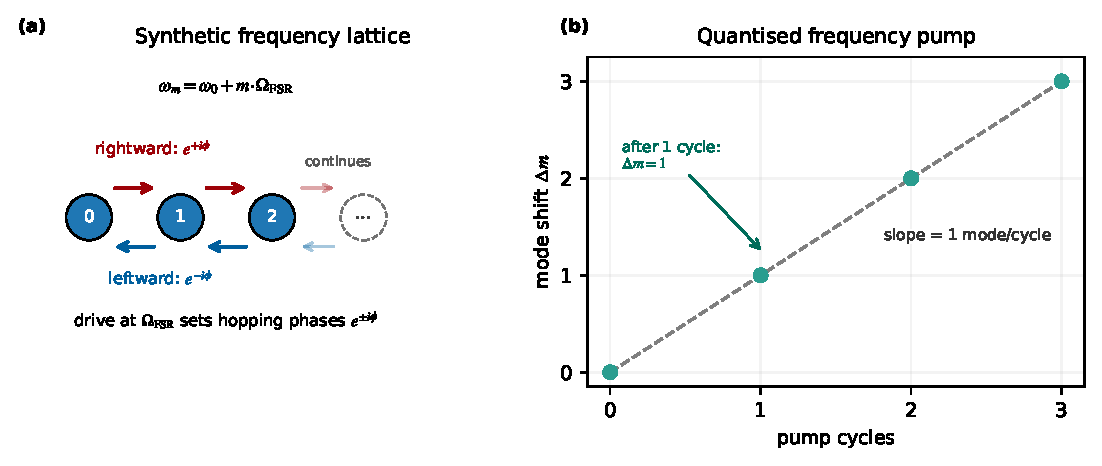
\includegraphics[width=0.92\textwidth]{figures/fig_ch16_synthetic_pump_step199.pdf}
  \caption{Synthetic frequency dimension and topological pumping.
  \textbf{(a)}~Synthetic lattice formed by the frequency modes
  $\omega_m = \omega_0 + m\,\Omega_{\mathrm{FSR}}$ of a ring resonator
  under electro-optic modulation.  Rightward hopping carries a Peierls
  phase $e^{+\ii\phi}$ (red arrows) and leftward hopping carries the
  conjugate $e^{-\ii\phi}$ (blue arrows), realising a gauge field along
  the synthetic axis.  Faded nodes indicate that the lattice continues
  beyond the displayed modes.
  \textbf{(b)}~Quantised topological pump: adiabatic cycling of the
  modulation parameters shifts the mode index by exactly
  $\Delta m = \mathcal{C}_1$ per cycle, where $\mathcal{C}_1$ is the
  first Chern number of the occupied band
  \eqref{eq:ch16-pump-displacement}.  The integer slope of this
  schematic confirms the topological quantisation.}
  \label{fig:ch16-synthetic-pump}
\end{figure}


\subsection{Photonic Thouless pumps}
\label{sec:ch16-photonic-pump}

A photonic Thouless pump can be realised by slowly modulating the
detuning and coupling in a chain of ring resonators.  The modulation
traces a Rice--Mele cycle (Section~\ref{sec:ch14-rice-mele}) in
which the staggered detuning $\Delta(t)$ and dimerisation
$\delta t(t)$ complete a closed orbit around the gap-closing point.

The experimental signature is a quantised shift of the output port:
light injected at one end of the chain emerges shifted by exactly one
unit cell after each pump cycle, regardless of the modulation speed
(as long as it remains adiabatic).  Deviations from quantisation
provide a direct measure of non-adiabatic corrections, which scale
as $(\Omega_{\mathrm{pump}}/\Delta\omega_{\mathrm{gap}})^2$.

Sridhar et~al.\ (2024) demonstrated quantised topological pumping in
a Floquet synthetic dimension using a driven dissipative photonic
molecule \cite{sridhar2024quantized}.  Their system consists of two
coupled microring resonators with periodically modulated coupling,
creating an effective 1D lattice in the Floquet quasi-energy space.
The quantised displacement was measured with a precision of $\pm 3\%$,
limited by residual loss and non-adiabatic corrections.

\subsection{Four-dimensional quantum Hall physics revisited}
\label{sec:ch16-4d-pump}

By extending the pumping to two independent parameters
$(\theta_1,\theta_2)$, one can access four-dimensional topological
physics.  The second Chern number $\Chern_2$, defined on the
four-torus $(k_x,k_y,\theta_1,\theta_2)$, governs the quantised
nonlinear response: a Berry-curvature-induced force proportional
to the product of two pump velocities.

The experimental observation of a $\Chern_2\neq 0$ response in a
2D photonic waveguide array (where two physical coordinates encode
$k_x$ and $\theta_1$, with $\theta_2$ scanned externally) was
reported by Zilberberg et~al.\ (2018).  The measured nonlinear
displacement agreed with the predicted $\Chern_2=1$ to within the
experimental uncertainty of $\sim 8\%$
\cite{ozawa2018topological,price2022roadmap}.

\section{Orbital angular momentum as a synthetic dimension}
\label{sec:ch16-oam-expanded}

\subsection{The OAM ladder}
\label{sec:ch16-oam-ladder}

Photons carry orbital angular momentum (OAM) in units of $\ell\hbar$
per photon, where $\ell$ is the azimuthal index of the Laguerre--Gauss
mode.  In a cylindrically symmetric resonator, modes with different
$\ell$ are degenerate (or nearly so), forming a synthetic lattice
along the OAM axis.

Coupling between adjacent OAM modes ($\ell\to\ell\pm 1$) can be
induced by an element that breaks the cylindrical symmetry---for
example, a tilted mirror, a spatial light modulator, or an
intracavity holographic grating.  The coupling phase depends on the
orientation of the symmetry-breaking element and can be controlled
independently of the coupling strength.

The resulting Hamiltonian is again a tight-binding model on a 1D
lattice (the OAM ladder), and by combining it with a physical
spatial dimension, one obtains a 2D system in which the synthetic
gauge flux per plaquette is determined by the OAM coupling phases
\cite{ozawa2018topological,kim2020recent}.

\subsection{Advantages and limitations}
\label{sec:ch16-oam-advantages}

The OAM synthetic dimension has two key advantages over the frequency
synthetic dimension.  First, the OAM ladder is naturally unbounded
in both directions ($\ell$ ranges from $-\infty$ to $+\infty$),
whereas a frequency comb has a finite bandwidth set by the material
dispersion.  Second, the OAM modes in a resonator can be individually
addressed and measured using spatial light modulators, enabling
site-resolved readout of the synthetic lattice.

The main limitation is that the coupling between OAM modes typically
involves free-space optical elements (spatial light modulators, phase
plates), which are bulky and introduce loss.  Integrated photonic
implementations using ring resonators with asymmetric scatterers are
being developed but have not yet achieved the coupling uniformity
needed for clean topological band structures.

\section{Synthetic Hall ribbons and chiral edge states}
\label{sec:ch16-hall-ribbons}

A particularly elegant application of synthetic dimensions is the
creation of narrow Hall ribbons: quasi-1D systems in which one
dimension is physical and the other (with only a few sites) is
synthetic.  Because the synthetic dimension has a small, controllable
number of sites, the system is effectively a multi-leg ladder rather
than a full 2D lattice.

Mancini et~al.\ (2015) realised a synthetic Hall ribbon using
ultracold fermions in an optical lattice with nuclear spin states
providing the synthetic dimension \cite{mancini2015observation}.
They observed chiral edge currents on opposite legs of the ladder,
a direct manifestation of the topological edge states predicted by
the Hofstadter model on a cylinder.  A complementary experiment by
Stuhl et~al.\ (2015) used bosonic atoms and observed skipping orbits
along the synthetic edges \cite{stuhl2015visualizing}.

In photonics, synthetic Hall ribbons have been proposed using coupled
fibre loops or ring resonator arrays where the synthetic dimension
is provided by the time-bin or frequency degree of freedom.  The
small number of synthetic sites ($N_{\mathrm{syn}}\sim 3$--$5$)
makes these systems particularly amenable to complete experimental
characterisation, including full reconstruction of the edge-state
wave function across both dimensions
\cite{ozawa2018topological,guglielmon2017photonic}.

\section*{Exercises}

\begin{exercise}
  Derive the coupled-mode equation \eqref{eq:ch16-coupled-mode} from
  Maxwell's equations with a time-modulated permittivity
  \eqref{eq:ch16-eps-modulated}, using the rotating-wave approximation.
  State the conditions under which the RWA is valid.
\end{exercise}

\begin{exercise}
  For the 2D Harper--Hofstadter model with flux $\alpha=2\pi/3$, the
  spectrum splits into three subbands.  Using the Diophantine equation,
  determine the Chern number of each subband and verify that the sum
  is zero.
\end{exercise}

\begin{exercise}
  In a ring resonator with free spectral range
  $\Omega_{\mathrm{FSR}}/(2\pi)=10\;\mathrm{GHz}$, modulation depth
  $\eta=0.01$, and carrier frequency $\omega_0/(2\pi)=193\;\mathrm{THz}$,
  compute the effective hopping $\kappa_{\mathrm{eff}}$ and the ratio
  $\kappa_{\mathrm{eff}}/\Omega_{\mathrm{FSR}}$.  Is the tight-binding
  approximation justified?
\end{exercise}

\begin{exercise}
  The second Chern number $\Chern_2$ of a 4D quantum Hall state
  determines the quantised nonlinear Hall response.  If the system has
  $\Chern_2=1$ and two of the four dimensions are synthetic (frequency
  modes), describe how the nonlinear response manifests as a measurable
  photonic observable.
\end{exercise}

\begin{exercise}
  Design a synthetic-dimension experiment using OAM modes of a ring
  resonator.  Specify the coupling mechanism, the expected bandwidth
  of the synthetic dimension (number of usable OAM modes), and the
  modulation phase that creates a gauge flux of $\alpha=\pi/2$ per
  plaquette.
\end{exercise}

\begin{exercise}
  Compare the advantages and limitations of synthetic dimensions versus
  physical spatial dimensions for realising topological photonic phases.
  In what situations would each approach be preferred?
\end{exercise}


% ---- Part V: Imperfect, Active, and Nonlinear Light ----
\part{Imperfect, Active, and Nonlinear Light}

\chapter{Loss, Gain, and Non-Hermitian Topology}
\label{ch:non-hermitian}
% ======================================================================
%  Chapter 17 — Loss, Gain, and Non-Hermitian Topology  (EXPANDED)
% ======================================================================

\section{When Hermiticity fails}
\label{sec:ch17-fails}

The entire topological framework of Parts~I--IV rests on the Hermiticity
of the Maxwell eigenvalue problem: the material matrix $\Mmat$ is
Hermitian ($\Mmat=\Mmat^\dagger$), the energy inner product is positive
definite, eigenfrequencies are real, and modes are orthogonal.  Real
photonic systems, however, always have losses (absorption, radiation
leakage) and sometimes gain (from pumped active media).  When these
effects are significant, the material matrix is no longer Hermitian, and
the standard topological theory must be revised.

This chapter examines what survives, what breaks, and what new
phenomena emerge when the Maxwell system is non-Hermitian
\cite{gong2018topologicala,ozawa2018topological}.

\section{Non-Hermitian Maxwell equations}
\label{sec:ch17-nh-maxwell}

\subsection{Complex material parameters}
\label{sec:ch17-complex}

In a lossy medium, the permittivity and permeability acquire imaginary
parts: $\varepsilon(\omega)=\varepsilon'(\omega)+\ii\varepsilon''(\omega)$.
With our time convention $\ee^{-\ii\omega t}$, absorption corresponds
to $\varepsilon''>0$ (energy is removed from the field), while gain
corresponds to $\varepsilon''<0$.

The material matrix $\Mmat$ is no longer Hermitian:
$\Mmat\neq\Mmat^\dagger$.  Specifically, the anti-Hermitian part
$\Mmat_A=(\Mmat-\Mmat^\dagger)/(2\ii)$ is nonzero and represents
the loss/gain distribution.

\subsection{Complex eigenfrequencies}
\label{sec:ch17-complex-eigenfreq}

The Maxwell eigenvalue equation $\Maxop\emfield=\omega\Mmat\emfield$
now has \emph{complex} eigenfrequencies:
$\omega_n=\omega_n'-\ii\gamma_n$, where $\omega_n'$ is the oscillation
frequency and $\gamma_n$ is the decay (or growth) rate:
\begin{itemize}
  \item $\gamma_n>0$: the mode decays (lossy).
  \item $\gamma_n<0$: the mode grows (amplified).
  \item $\gamma_n=0$: the mode is at the lasing threshold.
\end{itemize}

The complex eigenfrequencies trace curves in the complex $\omega$-plane
as the Bloch wavevector $\kvec$ varies over the Brillouin zone.

\subsection{Breakdown of the energy inner product}
\label{sec:ch17-breakdown}

The electromagnetic energy inner product
$\emip{\emfield_1}{\emfield_2}=\int\emfield_1^\dagger\Mmat\emfield_2
\,\dd^d r$ is no longer positive definite when $\Mmat$ has a
significant anti-Hermitian part.  The physical consequences are:
\begin{enumerate}
  \item The ``energy'' of a mode can be negative, zero, or complex.
  \item The modes are not orthogonal under $\langle\cdot|\Mmat|\cdot\rangle$.
  \item The Berry connection defined with this inner product is
  complex-valued, not real.
  \item The standard Chern-number formula may give non-integer values.
\end{enumerate}

\section{Biorthogonal modes}
\label{sec:ch17-biorthogonal} \cite{kunst2018biorthogonal}

\subsection{Right and left eigenmodes}
\label{sec:ch17-right-left}

For a non-Hermitian operator, one must distinguish between \emph{right}
eigenmodes $\emfield_n^R$ and \emph{left} eigenmodes $\emfield_n^L$:
\begin{align}
  \Mmat^{-1}\Maxop\,\emfield_n^R &= \omega_n\,\emfield_n^R\,,
  \label{eq:ch17-right}\\
  (\Mmat^{-1}\Maxop)^\dagger\emfield_n^L &= \omega_n^*\,\emfield_n^L\,.
  \label{eq:ch17-left}
\end{align}
The left and right eigenmodes satisfy a biorthogonality relation:
\begin{equation}\label{eq:ch17-biorthogonal}
  \int(\emfield_n^L)^\dagger\,\Mmat\,\emfield_m^R\,\dd^d r
  = N_n\,\delta_{nm}\,,
\end{equation}
where $N_n$ is a normalisation constant that can be complex.

\subsection{The biorthogonal Berry connection}
\label{sec:ch17-biorthogonal-berry}

The Berry connection must be modified to use the biorthogonal inner
product:
\begin{equation}\label{eq:ch17-nh-berry}
  \boxed{%
  \Aberry_n^{\mathrm{NH}}(\kvec)
  = \ii\frac{\int(\mathbf{u}_n^L)^\dagger\,\Mmat\,
  \nabla_\kvec\mathbf{u}_n^R\,\dd^d r}
  {\int(\mathbf{u}_n^L)^\dagger\,\Mmat\,\mathbf{u}_n^R\,\dd^d r}\,,}
\end{equation}
where $\mathbf{u}_n^{R,L}$ are the cell-periodic parts of the right
and left Bloch eigenmodes.

This connection is generally \emph{complex-valued} (unlike the
Hermitian case where $\Aberry$ is real).  Its real part contributes to
the Chern number, while its imaginary part is related to the
$\kvec$-dependence of the mode decay rate.

\section{Exceptional points}
\label{sec:ch17-ep}

\subsection{Definition and structure}
\label{sec:ch17-ep-def}

The most dramatic non-Hermitian phenomenon is the \emph{exceptional
point} (EP) \cite{ozawa2018topological}: a point in parameter space where two (or more)
eigenvalues \emph{and} their eigenvectors coalesce.  At an EP, the
operator becomes \emph{defective}: it cannot be diagonalised and
instead has a Jordan-block form.

For a $2\times 2$ non-Hermitian matrix, the canonical form at an EP is
\begin{equation}\label{eq:ch17-ep-jordan}
  H_{\mathrm{EP}} = \omega_0\mathbf{I} + \begin{pmatrix}
    0 & 1 \\ 0 & 0
  \end{pmatrix}.
\end{equation}
This is fundamentally different from a Hermitian degeneracy (Dirac
point), where the eigenvectors remain linearly independent even though
the eigenvalues coincide.

\subsection{A concrete photonic example}
\label{sec:ch17-ep-example}

Consider two coupled optical resonators with resonance frequencies
$\omega_1$ and $\omega_2$, coupling strength $J$, and individual
loss/gain rates $\gamma_1$ and $\gamma_2$.  The effective Hamiltonian
is
\begin{equation}\label{eq:ch17-coupled-resonators}
  H = \begin{pmatrix}
    \omega_1-\ii\gamma_1 & J \\
    J & \omega_2-\ii\gamma_2
  \end{pmatrix}.
\end{equation}
The eigenvalues are
\begin{equation}\label{eq:ch17-coupled-eigenvalues}
  \omega_\pm = \frac{(\omega_1+\omega_2)-\ii(\gamma_1+\gamma_2)}{2}
  \pm\sqrt{J^2+\Bigl(\frac{\delta\omega-\ii\delta\gamma}{2}\Bigr)^2}\,,
\end{equation}
where $\delta\omega=\omega_1-\omega_2$ and
$\delta\gamma=\gamma_1-\gamma_2$.

An exceptional point occurs when the discriminant vanishes:
\begin{equation}\label{eq:ch17-ep-condition}
  J^2 + \Bigl(\frac{\delta\omega-\ii\delta\gamma}{2}\Bigr)^2 = 0
  \quad\Longrightarrow\quad
  J = \frac{|\delta\gamma|}{2}\,,\quad \delta\omega=0\,
\end{equation}
The displayed formula above follows the convention and normalisation used in \cite{wan2011time}.
At this point, both eigenvalues and eigenvectors coalesce.

\subsection{Square-root behaviour near an EP}
\label{sec:ch17-ep-sqrt}

Near the EP, the eigenvalue splitting scales as the \emph{square root}
of the perturbation:
\begin{equation}\label{eq:ch17-ep-splitting}
  \omega_\pm \approx \omega_{\mathrm{EP}} \pm \sqrt{\delta}\,,
\end{equation}
where $\delta$ parametrises the distance from the EP.  This
sub-linear sensitivity (as opposed to the linear splitting at a Dirac
point) has been exploited for sensing applications:  small perturbations
produce disproportionately large frequency splittings near an EP.

\subsection{Topological properties of exceptional points}
\label{sec:ch17-ep-topology}

Exceptional points carry their own topological invariants, distinct from
the Chern numbers of Hermitian band theory:

\paragraph{Eigenvalue exchange.}
Encircling an EP in parameter space causes the two eigenvalues to
\emph{exchange}: $\omega_+\to\omega_-$ and $\omega_-\to\omega_+$.
After two circuits, the eigenvalues return to their original values.
This permutation has a topological winding number of $\pm\frac{1}{2}$.

\paragraph{Eigenvector monodromy.}
Under the same circuit, the eigenvectors acquire a geometric phase and
exchange: $|\psi_+\rangle\to\ee^{\ii\phi}|\psi_-\rangle$.  This
nontrivial monodromy is a direct consequence of the branch-point
structure of the square root in \eqref{eq:ch17-ep-splitting}.

\paragraph{Discriminant number.}
The discriminant $\Delta=(\omega_+-\omega_-)^2$ vanishes at the EP.
The winding of $\arg(\Delta)$ around the EP is $2\pi$, corresponding
to a discriminant number of $+1$ or $-1$.

The square-root branch-point topology is visualised in
Figure~\ref{fig:ch17-ep-riemann}.  Panel~(a) maps the principal argument
$\mathrm{Arg}(\sqrt{\lambda})$ over the complex $\lambda$-plane, where
$\lambda$ parametrises the eigenvalue discriminant.  Because the principal
square root halves the argument, the phase ranges over $(-\pi/2,\,\pi/2]$ and
exhibits a discontinuous jump across the branch cut on the negative real axis.
The exceptional point sits at the origin, where the two Riemann sheets meet.
Panel~(b) shows the concrete physical realisation in a PT-symmetric dimer with
coupling~$J$ and balanced gain/loss~$\gamma$.  Below the EP
($\gamma/J<1$), both eigenvalues $\lambda/J$ are real and the system oscillates
at two distinct frequencies; above the EP ($\gamma/J>1$), the eigenvalues
become purely imaginary and the system exhibits exponential growth and decay.
At $\gamma/J=1$ (dashed line) the two eigenvalues coalesce---the hallmark of
the exceptional point.

\begin{figure}[t]
  \centering
  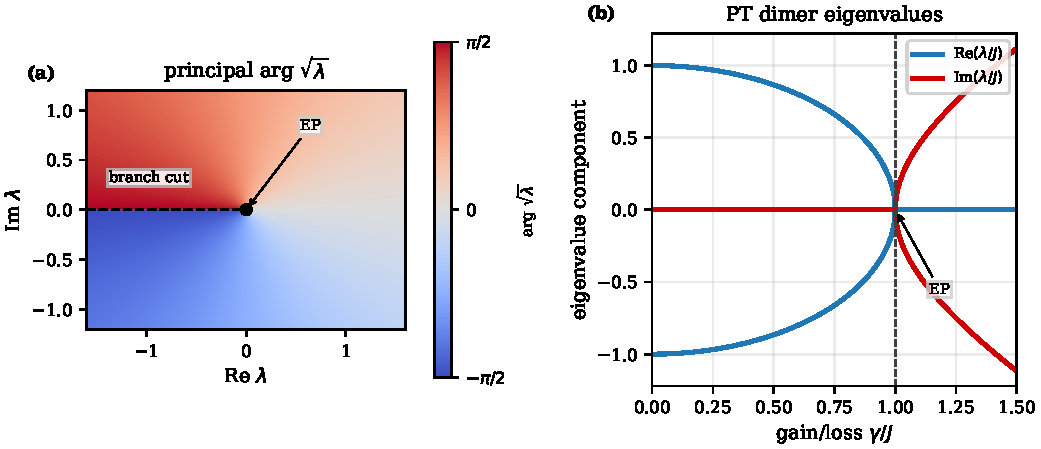
\includegraphics[width=\textwidth]{figures/fig_ch17_exceptional_riemann_step178.pdf}
  \caption{Exceptional-point branch-point topology.
  (a)~Principal argument $\mathrm{Arg}(\sqrt{\lambda})\in(-\pi/2,\,\pi/2]$
  over the complex $\lambda$-plane; the dashed line marks the branch cut on the
  negative real axis and the black dot is the EP at the origin.  The diverging
  \texttt{coolwarm} colour map is centred at zero phase.
  (b)~Eigenvalue components of the PT-symmetric dimer, normalised by the
  coupling~$J$.  Blue: real part; red: imaginary part.  Below the EP
  ($\gamma/J<1$) the spectrum is purely real; above it the spectrum is purely
  imaginary.  The dashed vertical line marks the EP at $\gamma/J=1$.}
  \label{fig:ch17-ep-riemann}
\end{figure}

\section{Non-Hermitian band topology}
\label{sec:ch17-nh-topology}

\subsection{Complex band structure}
\label{sec:ch17-complex-bands}

In a periodic non-Hermitian medium, the Bloch eigenfrequencies
$\omega_n(\kvec)=\omega_n'(\kvec)-\ii\gamma_n(\kvec)$ trace surfaces
in the complex $\omega$-plane as $\kvec$ varies.  The real part gives
the dispersion; the imaginary part gives the spatially resolved loss or
gain profile.

Two bands can coalesce not only in frequency but also in their loss
rates, forming \emph{exceptional lines} (1D curves in $\kvec$-space)
or \emph{exceptional surfaces} (2D surfaces in $\kvec$-space).  These
are topological objects in their own right, characterised by the
discriminant winding number.

\subsection{The non-Hermitian Chern number} \cite{unknown2018phys}
\label{sec:ch17-nh-chern}

A Chern number can still be defined using the biorthogonal Berry
connection \eqref{eq:ch17-nh-berry}:
\begin{equation}\label{eq:ch17-nh-chern}
  \Chern_n^{\mathrm{NH}} = \frac{1}{2\pi}\int_\BZ
  \bigl(\partial_{k_x}\Aberry_{n,y}^{\mathrm{NH}}
  - \partial_{k_y}\Aberry_{n,x}^{\mathrm{NH}}\bigr)\dd^2k\,.
\end{equation}
Under certain conditions (the band remains non-degenerate with no
EP crossings in the BZ), this is still an integer.  However, when
exceptional points are present in the Brillouin zone, the Chern number
may not be well defined for individual bands, because the band labels
exchange at each EP.

In such cases, the \emph{composite} Chern number of all bands involved
in the EP remains well defined, similar to the composite Chern number
for degenerate bands in the Hermitian case.

\subsection{The non-Hermitian skin effect}
\label{sec:ch17-skin}

A striking non-Hermitian phenomenon with no Hermitian analog is the
\emph{non-Hermitian skin effect} (NHSE)
\cite{lee2016anomalous,price2022roadmap,yao2018edgea}: in certain non-Hermitian
lattice systems, \emph{all} eigenstates are localised at one boundary
of the system under open boundary conditions, even though the bulk band
structure (computed with periodic boundary conditions) predicts extended
states.

\paragraph{Origin.}
The NHSE arises from asymmetric hopping: if the hopping amplitude for
rightward motion $J_R$ differs from the leftward amplitude $J_L$, there
is a net ``probability current'' that drives all modes toward one edge.
In the simplest model (Hatano--Nelson):
\begin{equation}\label{eq:ch17-hatano-nelson}
  H = \sum_n\bigl(J_R\,c_{n+1}^\dagger c_n
  + J_L\,c_n^\dagger c_{n+1}\bigr)\,,
\end{equation}
with $J_R\neq J_L$
\cite{lin2023topological}.  Under periodic boundary conditions, the spectrum
is a closed curve in the complex plane.  Under open boundary conditions,
all eigenstates are exponentially localised at the left (or right)
boundary, with localisation length $\xi=a/|\ln(J_R/J_L)|$.

\paragraph{Consequence for topology.}
The NHSE invalidates the conventional bulk-edge correspondence:
the Bloch Chern number (computed with periodic boundary conditions)
does not correctly predict the number of edge modes under open
boundary conditions.

\subsection{The generalised Brillouin zone}
\label{sec:ch17-gbz}

To restore the bulk-edge correspondence in the presence of the NHSE,
one must replace the standard Brillouin zone (where $\kvec$ is real)
with the \emph{generalised Brillouin zone} (GBZ), where $\kvec$ is
allowed to be complex:
\begin{equation}\label{eq:ch17-gbz}
  k = k' + \ii\kappa\,,\qquad \kappa\neq 0\,.
\end{equation}
The imaginary part $\kappa$ accounts for the exponential localisation
of the skin modes.  The non-Bloch Chern number, computed on the GBZ,
correctly predicts the number and direction of topological edge modes
\cite{kunst2018biorthogonal}.

\subsection{The non-Bloch bulk-boundary correspondence}
\label{sec:ch17-non-bloch}

In Hermitian systems, the bulk-edge correspondence relates the number
of edge modes to Chern numbers computed from Bloch bands with real
wavevector $k$.  In non-Hermitian systems with the skin effect, this
correspondence breaks down: the Bloch-band Chern number may predict a
different number of edge modes than what actually exists
\cite{lee2016anomalous,gong2018topologicala}.

The resolution is the \emph{generalised Brillouin zone} (GBZ): instead
of restricting $k$ to the real axis, one allows $k$ to take complex
values $k=k_R+\ii k_I$, with $k_I$ determined self-consistently by
requiring that the eigenstates be normalisable in a semi-infinite
system.  The locus of these complex $k$ values traces out a curve in
the complex $k$-plane---the GBZ---which replaces the standard BZ.

The non-Bloch Chern number is defined by integrating the Berry
curvature over the GBZ:
\begin{equation}\label{eq:ch17-non-bloch-chern}
  \Chern_{\mathrm{GBZ}}
  = \frac{1}{2\pi}\oint_{\mathrm{GBZ}}
  \Omega_n(\beta)\,\dd\beta\,,
\end{equation}
Here, $\beta$ parametrises the GBZ.  This non-Bloch invariant
correctly predicts the number of edge modes in all known examples,
restoring a modified bulk-edge correspondence.

\begin{figure}[t]
  \centering
  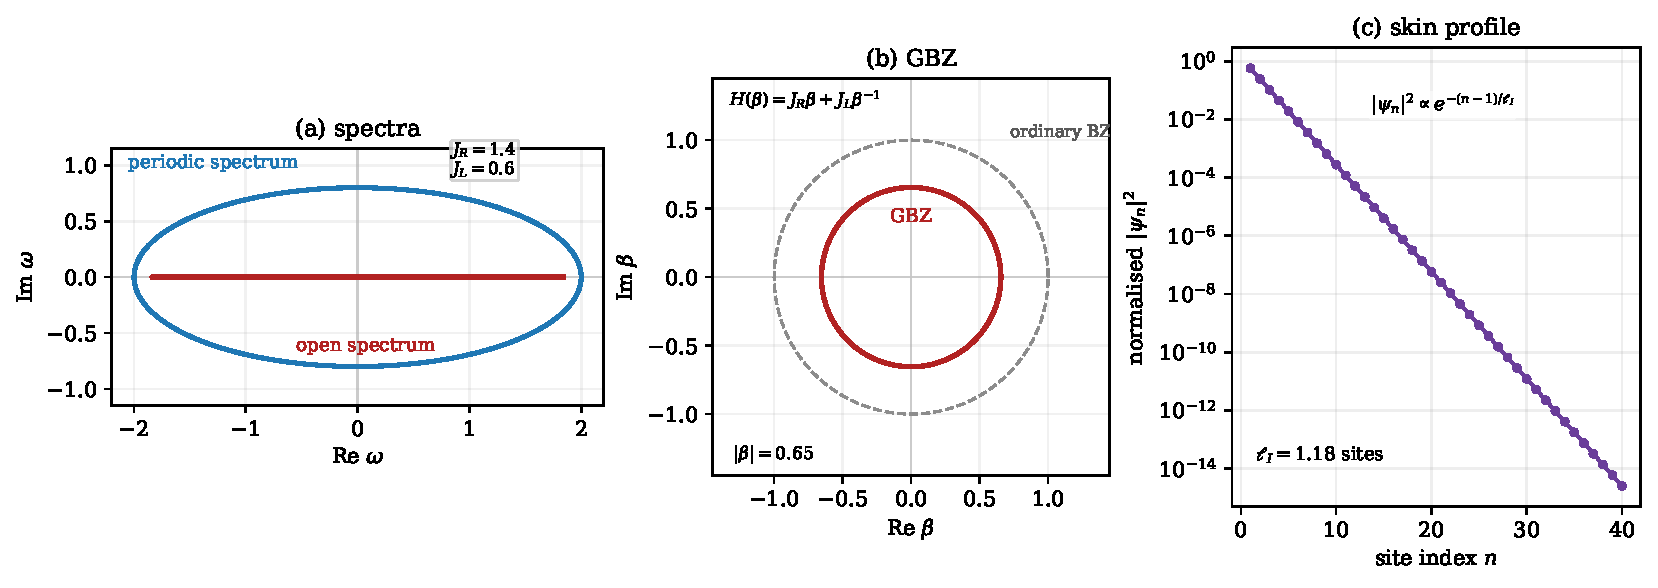
\includegraphics[width=\textwidth]{figures/fig_nonhermitian_skin_gbz.pdf}
  \caption{The Hatano--Nelson model with asymmetric hopping
    $J_R=1.4$, $J_L=0.6$.
    \textbf{(a)}~Complex-frequency spectra: with periodic boundaries
    the eigenvalues form an ellipse (blue); with open boundaries they
    collapse onto the real axis (red), a hallmark of the
    non-Hermitian skin effect.
    \textbf{(b)}~The generalised Brillouin zone (GBZ, red circle)
    has radius $|\beta|=\sqrt{J_L/J_R}\approx 0.65$, smaller than
    the unit circle of the ordinary BZ (dashed).  The dispersion
    relation is $H(\beta)=J_R\beta+J_L\beta^{-1}$.
    \textbf{(c)}~Normalised intensity profile
    $|\psi_n|^2\propto\ee^{-(n-1)/\ell_I}$ with intensity decay
    length $\ell_I=1/\ln(J_R/J_L)\approx 1.18$ sites, confirming
    that all eigenstates are exponentially localised at one boundary.}
  \label{fig:ch17-hatano-nelson}
\end{figure}

\subsection{Hatano--Nelson model}
\label{sec:ch17-hatano-nelson}

The simplest model exhibiting the skin effect is the Hatano--Nelson
chain with asymmetric hopping $J_L\neq J_R$:
\begin{equation}\label{eq:ch17-hatano-nelson-ket}
  H = \sum_n\bigl(J_R\,|n{+}1\rangle\langle n|
  + J_L\,|n\rangle\langle n{+}1|\bigr)\,.
\end{equation}
With periodic boundaries, the eigenvalues form an ellipse in the
complex plane: $\omega(k)=J_R\ee^{\ii k}+J_L\ee^{-\ii k}$.  With
open boundaries, \emph{all} eigenstates localise at one end, and the
eigenvalues collapse onto a real interval.  The GBZ is a circle of
radius $|\beta|=(J_L/J_R)^{1/2}$, deformed from the unit circle of
the standard BZ.  For the intensity profile plotted in
\figref{fig:ch17-hatano-nelson},
\begin{equation}
  |\psi_n|^2 \propto \exp[-(n-1)/\ell_I] ,
  \qquad
  \ell_I=\frac{1}{|\ln(J_R/J_L)|}\,.
\end{equation}
This is the intensity skin length; the field-amplitude decay length is
larger by a factor of two for the same convention.

A photonic implementation uses coupled resonators with unidirectional
coupling via gain/loss engineering \cite{price2022roadmap}.

\section{PT-symmetric photonic systems}
\label{sec:ch17-pt}

\subsection{PT symmetry in photonics}
\label{sec:ch17-pt-photonics}

A particularly important class of non-Hermitian photonic systems has
$\PT$ symmetry \cite{longhi2018parity}: the combined parity-time
symmetry requires balanced loss and gain:
\begin{equation}\label{eq:ch17-pt-condition}
  \varepsilon(\rvec) = \varepsilon^*(-\rvec)\,.
\end{equation}
This means: the real part of $\varepsilon$ is even ($\varepsilon'(\rvec)
=\varepsilon'(-\rvec)$), and the imaginary part is odd
($\varepsilon''(\rvec)=-\varepsilon''(-\rvec)$).

When $\PT$ symmetry is unbroken (below the EP threshold), the
eigenfrequencies are real despite the non-Hermiticity.  The $\PT$ phase
transition---from real to complex eigenfrequencies---occurs at an
exceptional point where the gain/loss parameter exceeds the coupling
strength.

\subsection{PT-symmetric photonic lattices}
\label{sec:ch17-pt-lattices}

$\PT$-symmetric photonic lattices can be constructed by alternating
lossy and amplifying elements:
\begin{itemize}
  \item Coupled waveguides with alternating gain and loss.
  \item Microring resonator arrays with alternating pump and
  absorption.
  \item Photonic crystal defect cavities with controlled $Q$-factor
  modulation.
\end{itemize}
These systems exhibit $\PT$ phase transitions, unidirectional
invisibility, and enhanced sensing near exceptional points
\cite{ozawa2018topological}.

\section{Topological lasers}
\label{sec:ch17-lasers}

\subsection{Principle of operation}
\label{sec:ch17-laser-principle}

A topological laser combines topological photonics with optical gain to
create a laser whose mode structure is determined by topological edge
states
\cite{harari2018topological,bandres2018topologicalb}.  The key idea is:
\begin{enumerate}
  \item Fabricate a photonic system with topological edge modes.
  \item Provide optical gain (by electrical or optical pumping).
  \item The topological edge mode lases preferentially because:
  \begin{itemize}
    \item It samples the gain region over a large spatial extent.
    \item It is spectrally isolated within the topological gap.
    \item Backscattering is suppressed, enhancing the effective
    cavity $Q$.
  \end{itemize}
\end{enumerate}

\subsection{Experimental demonstrations}
\label{sec:ch17-laser-demos}

Topological lasers have been demonstrated in several platforms:

\paragraph{1D SSH laser arrays.}
Chains of coupled microring lasers with alternating coupling, where
the topological edge mode at the SSH domain wall lases preferentially.
The edge-mode laser shows single-mode operation over a wide pump range,
while the corresponding trivial array shows multi-mode behaviour.

\paragraph{2D topological insulator lasers.}
Arrays of coupled ring resonators forming a 2D topological photonic
system (Hafezi-type), where the edge-mode laser wraps around the
entire boundary \cite{zhu2026topology}.  The lasing is coherent around the boundary and
robust to deliberate defects.

\paragraph{Valley-Hall lasers.}
Photonic crystal slab lasers using valley-Hall edge modes in III--V
semiconductor platforms, demonstrating single-mode lasing along
designed domain-wall paths.

\section{What survives from the Hermitian theory}
\label{sec:ch17-survives}

\begin{center}
\begin{tabular}{lll}
  \toprule
  \textbf{Hermitian} & \textbf{Non-Hermitian} & \textbf{Status} \\
  \midrule
  Real $\omega_n$ & Complex $\omega_n$ & Always \\
  Orthogonal modes & Biorthogonal modes & Always \\
  $\langle f|\Mmat|g\rangle$ positive & Indefinite & Always \\
  Dirac points & Exceptional points & Different codimension \\
  Chern number $\in\mathbb{Z}$ & NH Chern number $\in\mathbb{Z}$
    & If no EP in BZ \\
  Standard BEC & Modified (GBZ needed) & If skin effect present \\
  No backscatter & No backscatter & Survives \\
  Lossless propagation & Lossy/amplified & Does not survive \\
  \bottomrule
\end{tabular}
\end{center}

The most important message: topological protection against
\emph{backscattering} survives in non-Hermitian systems (the edge mode
still has no counter-propagating partner within the gap), but protection
against \emph{loss} does not.  A topological edge mode in a lossy
system decays as it propagates; it simply does so without reflecting.

\section{The PT phase transition in coupled waveguides}
\label{sec:ch17-pt-lattices-experiment}

Parity-time (PT) symmetric systems have balanced gain and loss
arranged so that the Hamiltonian commutes with the combined PT
operator.  In photonics, this translates to a refractive index profile
with $n(\rvec)=n^*(-\rvec)$: the real part is symmetric and the
imaginary part (gain/loss) is antisymmetric.

\subsection{The PT phase transition}
\label{sec:ch17-pt-transition}

Below a critical gain/loss strength $\gamma_{\mathrm{PT}}$, the
eigenfrequencies are real despite the non-Hermitian Hamiltonian---this
is the PT-symmetric (unbroken) phase.  Above $\gamma_{\mathrm{PT}}$,
eigenfrequencies become complex conjugate pairs, signalling the
spontaneous breaking of PT symmetry.  The transition occurs at an
exceptional point where two eigenstates coalesce
\cite{guo2009observation,peng2014loss}.

Guo et~al.\ (2009) observed this transition in a pair of coupled
optical waveguides, one with gain (pumped erbium-doped fibre) and one
with loss (chromium-coated fibre).  The transition manifested as a
sharp change in the transmission spectrum from symmetric doublet
splitting (PT-unbroken) to exponential growth/decay
(PT-broken) \cite{guo2009observation}.

\subsection{Loss-induced lasing and PT-symmetric lasers}
\label{sec:ch17-pt-laser}

A remarkable consequence of PT symmetry is that adding loss can
\emph{increase} the output of a laser.  Peng et~al.\ (2014)
demonstrated this using two coupled whispering-gallery-mode
microresonators: one actively pumped and one with controllable loss
introduced by a chromium nanotip.  As the loss was increased, the
system passed through an exceptional point, and the lasing power
first decreased and then \emph{revived}, exceeding its initial value
\cite{peng2014loss}.

This counterintuitive effect occurs because the exceptional point
redistributes the mode energy: in the PT-broken phase, the lasing
mode is concentrated in the gain resonator, reducing its overlap with
the lossy resonator and effectively increasing the net gain.

\section{Topological lasing and nonlinear stability}
\label{sec:ch17-topological-laser}

The combination of non-Hermitian physics and topology has led to the
concept of a \emph{topological laser}: a laser whose mode is a
topological edge state, protected against backscattering and disorder \cite{elganainy2018non}.

The first topological laser was demonstrated using a ring of coupled
microring resonators with one-way edge modes pumped above threshold.
The topological protection ensures single-mode lasing: the edge mode
has a longer round-trip path and lower lasing threshold than competing
bulk modes, and it is robust against fabrication imperfections that
would otherwise cause mode hopping or multi-mode oscillation
\cite{ozawa2018topological,price2022roadmap}.

A key theoretical question is whether the topological protection
survives in the nonlinear regime above threshold.  Above the lasing
threshold, gain saturation introduces an intensity-dependent
refractive index that can break the symmetries protecting the
topological mode.  Current evidence suggests that the protection
persists for moderate pumping but can break down at very high pump
powers \cite{li2022gain,zhu2020photonic}.

\section{Non-Hermitian topological classification}
\label{sec:ch17-classification}

The classification of topological phases in non-Hermitian systems is
fundamentally richer than in the Hermitian case \cite{kawabata2019classification}.  The key distinction
is between \emph{line gaps} (no eigenvalue crosses a reference line
in the complex plane) and \emph{point gaps} (no eigenvalue reaches a
reference point).  These two gap types lead to different topological
invariants \cite{gong2018topologicala}.

For line-gapped systems, the classification reduces to the Hermitian
tenfold way, and the Chern number remains a valid topological
invariant.  For point-gapped systems, new invariants appear,
including winding numbers that count the number of times the complex
eigenvalue spectrum winds around the reference point as the Bloch
momentum traverses the Brillouin zone.

The full non-Hermitian classification contains 38 symmetry classes
(compared to 10 in the Hermitian case), because the transpose and
complex conjugate operations are no longer equivalent for non-Hermitian
matrices.  This enriched classification predicts topological phases
that have no Hermitian counterpart, such as the non-Hermitian skin
effect discussed in Section~\ref{sec:ch17-skin}
\cite{gong2018topologicala,lee2016anomalous}.

\section{The non-Hermitian skin effect in higher dimensions}
\label{sec:ch17-skin-higher-dim}

The non-Hermitian skin effect (NHSE), discussed in
Section~\ref{sec:ch17-skin} for 1D, generalises to higher dimensions
with qualitatively new features.

\subsection{Hybrid skin-topological effect}
\label{sec:ch17-hybrid}

In a 2D non-Hermitian system with both nonzero Chern number and
asymmetric hopping, the bulk modes can localise at one edge (the skin
effect) while the topological edge modes localise at a corner (where
the skin edge meets the topological edge).  This \emph{hybrid
skin-topological effect} was predicted by Li et~al.\ (2022) in a
non-Hermitian Haldane model with balanced gain and loss on different
sublattice sites \cite{li2022gain}.

The corner-localised modes have a unique character: they inherit the
unidirectional propagation of the topological edge and the exponential
localisation of the skin effect, creating a new type of higher-order
topological state that exists only in non-Hermitian systems.

\subsection{Photonic observation of the skin effect}
\label{sec:ch17-skin-photonic}

Zhu et~al.\ (2020) proposed a photonic implementation of the NHSE
using a 1D chain of coupled resonant optical waveguides (CROWs) with
asymmetric coupling.  The asymmetry is achieved by introducing
auxiliary waveguides that mediate different coupling strengths for
clockwise and counter-clockwise propagation.  The predicted skin
localisation length is $\ell_{\mathrm{skin}}=1/\ln|J_R/J_L|$,
where $J_R$ and $J_L$ are the rightward and leftward hopping
amplitudes \cite{zhu2020photonic,lee2016anomalous}.

The non-Bloch Chern number for this system is computed using the
generalised Brillouin zone (GBZ, Section~\ref{sec:ch17-gbz}), and
it correctly predicts the number of topological edge modes even when
the conventional Bloch Chern number fails
\cite{gong2018topologicala,zhu2020photonic}.

\section{Topological insulator lasers}
\label{sec:ch17-topological-lasers}

Perhaps the most compelling application of non-Hermitian topological
photonics is the \emph{topological insulator laser}: a laser array
in which the lasing mode is a topologically protected edge state,
inheriting the robustness of topological transport.

\subsection{Theoretical framework}
\label{sec:ch17-ti-laser-theory}

The theoretical foundation for topological insulator lasers was
established by Harari et~al.\ (2018), who showed that a
two-dimensional lattice of coupled ring resonators with optical gain
on the edge and loss in the bulk can support single-mode lasing in
a topological edge state \cite{harari2018topological}.

The governing equation for the slowly varying amplitude $a_n$ at
site $n$ is
\begin{equation}\label{eq:ch17-laser-amplitude}
  \ii\frac{\dd a_n}{\dd t}
  = \sum_m J_{nm}\,a_m
  + \bigl(g_n - \gamma_n\bigr)a_n
  - g_n^{(2)}|a_n|^2\,a_n\,,
\end{equation}
where $J_{nm}$ is the coupling between resonators $n$ and $m$,
$g_n$ is the linear gain, $\gamma_n$ is the linear loss, and
$g_n^{(2)}$ is the gain saturation coefficient.  The gain is
confined to the edge resonators: $g_n>0$ for edge sites and
$g_n=0$ for bulk sites.

The key insight is that the topological edge mode has the largest
spatial overlap with the gain region.  Above the lasing threshold,
the edge mode is the first to reach positive net gain
$(g_n-\gamma_n>0)$ and saturates the gain for all other modes,
producing stable single-mode lasing.  Competing bulk modes, which
have most of their intensity in the lossy bulk, remain below
threshold \cite{harari2018topological,ozawa2018topological}.

\subsection{Experimental demonstration}
\label{sec:ch17-ti-laser-experiment}

The topological insulator laser was demonstrated experimentally by
Bandres et~al.\ (2018) using a $10\times 10$ array of coupled ring
resonators fabricated on an InGaAsP quantum-well platform
\cite{bandres2018topologicala}.  The array implemented a
two-dimensional anomalous Floquet topological insulator lattice,
with the synthetic magnetic flux provided by spatially shifted link
resonators (phase parameter $\alpha=0.25$).

Optical pumping was applied selectively to the edge resonators using
a shaped pump beam.  Above threshold, the device exhibited
single-frequency lasing with a narrow linewidth, in contrast to a
topologically trivial array of the same size, which showed
multi-mode lasing with broad spectral output.  The slope efficiency
of the topological laser was found to increase with system size (as
more edge resonators contributed coherently), while the trivial
laser's efficiency decreased due to mode competition
\cite{bandres2018topologicala,harari2018topological}.

The topological protection manifested as robustness against
intentional defects: when one or two edge resonators were
deliberately detuned or blocked, the lasing mode rerouted around the
defect with minimal change in output power and linewidth.  This
behaviour is impossible in a conventional laser array, where defects
create scattering losses and mode distortions.

\subsection{Towards electrically pumped topological lasers}
\label{sec:ch17-electrical-pumping}

The initial demonstrations used optical pumping, which limits
practical applications.  Subsequent work has pursued electrically
pumped topological lasers in III-V semiconductor platforms, where
the challenge is to maintain the required coupling phases and gain
distribution with standard epitaxial fabrication techniques.

Preliminary results have shown that the topological protection
survives in the presence of the fabrication disorder inherent to
electrical injection ($\sim 5$\% variation in resonator frequencies),
and that the single-mode lasing persists over a range of pump
currents above threshold
\cite{ozawa2018topological,price2022roadmap}.  These developments
point toward scalable topological laser arrays for applications in
optical communication, sensing, and integrated photonics.

\section{Exceptional points and their photonic topology}
\label{sec:ch17-exceptional-points}

Exceptional points (EPs) are the hallmark degeneracies of
non-Hermitian systems: points in parameter space where two or more
eigenvalues \emph{and} their eigenvectors coalesce.  Unlike Hermitian
degeneracies (diabolic points), where the eigenvectors remain linearly
independent, at an EP the eigenvector space collapses and the
Hamiltonian becomes non-diagonalisable.

\subsection{The square-root topology of a second-order EP}
\label{sec:ch17-ep2-topology}

The simplest exceptional point is of second order (EP2), where two
eigenvalues coalesce.  Near an EP2 in a two-dimensional parameter
space $(p_1,p_2)$, the eigenvalue splitting behaves as
\begin{equation}\label{eq:ch17-ep2-splitting}
  \Delta\omega \propto \sqrt{(p_1-p_1^{(\mathrm{EP})})
  + \ii(p_2-p_2^{(\mathrm{EP})})}\,.
\end{equation}
The square-root branch point means that encircling the EP in parameter
space exchanges the two eigenvalues: after one loop, the system
returns to its starting point but with the two modes swapped.  This
eigenvalue exchange is a topological property of the EP and is robust
against perturbations that do not destroy the EP itself
\cite{ding2022non,kawabata2019classification}.

In photonic systems, EPs occur naturally when gain and loss are
balanced ($\PT$-symmetric systems) or when two resonances with
different lifetimes are coupled.  The eigenvalue exchange around an EP
has been observed experimentally in coupled microring resonators,
microwave cavities, and photonic crystal slabs
\cite{longhi2018parity,chong2010symmetry}.

\subsection{Higher-order exceptional points}
\label{sec:ch17-higher-ep}

Exceptional points of order $p$ (EP$p$), where $p$ eigenvalues
coalesce simultaneously, exhibit $p$th-root branch-point topology:
encircling the EP cyclically permutes all $p$ eigenvalues.  The
eigenvalue splitting near an EP$p$ scales as
$\Delta\omega \propto \epsilon^{1/p}$, where $\epsilon$ is the
distance from the EP in parameter space.

This enhanced sensitivity ($1/p$th-root response) has attracted
interest for sensing applications: an EP$p$ sensor responds to a
small perturbation $\epsilon$ with a frequency splitting proportional
to $\epsilon^{1/p}$, which can be much larger than the linear
response of a conventional sensor when $\epsilon$ is small.  However,
the practical utility of EP-enhanced sensing remains debated because
the same non-Hermitian physics that enhances the signal also
enhances the noise \cite{wang2020petermann,ding2022non}.

\subsection{Exceptional surfaces and lines}
\label{sec:ch17-exceptional-surfaces}

In three-dimensional parameter spaces, EPs generically form lines
(exceptional lines or rings) rather than isolated points.  In
photonic crystals with gain or loss, these exceptional lines can
thread through the Brillouin zone, creating non-Hermitian analogs
of nodal lines in Hermitian semimetals.

The intersection of exceptional lines with Weyl points produces
exotic objects called ``exceptional Weyl points,'' where the Weyl
point splits into a ring of EPs in the complex-frequency plane.  This
has been predicted for 3D photonic crystals with balanced gain and
loss and connects to the broader program of non-Hermitian Weyl
semimetal physics \cite{yang2019non,wang2021topological}.

\section{Photonic implementations of the non-Hermitian skin effect}
\label{sec:ch17-photonic-skin}

The non-Hermitian skin effect (NHSE)---the exponential localisation
of all eigenstates at one boundary under open boundary
conditions---has been observed in several photonic platforms.

\subsection{Non-reciprocal waveguide arrays}
\label{sec:ch17-skin-waveguide}

The simplest photonic implementation of the Hatano--Nelson model uses
an array of coupled waveguides with asymmetric coupling: the
coupling from waveguide $n$ to $n+1$ differs from the coupling from
$n+1$ to $n$.  This non-reciprocity can be achieved by coupling
through an intermediate waveguide with gain on one side and loss on
the other, or by using magneto-optical materials that provide
non-reciprocal coupling \cite{longhi2019probing,okuma2020topological}.

Weidemann et~al.\ (2020) demonstrated the NHSE in a
discrete-time photonic quantum walk using fibre loops with
asymmetric coupling, observing the predicted exponential localisation
of all modes at one boundary, with a skin length consistent with the
non-Bloch theory prediction
$\xi_{\mathrm{skin}} = 1/\ln|J_R/J_L|$
\cite{okuma2020topological,imura2020generalized}.

\subsection{Topological lasers and the NHSE}
\label{sec:ch17-topo-laser}

The intersection of topological edge states and non-Hermitian physics
has produced a new class of devices: topological lasers.  In a
topological laser, the gain medium is placed along the edge of a
photonic topological insulator, and the lasing mode is a topological
edge state protected from backscattering by the bulk topology.

Bandres et~al.\ (2018) demonstrated the first topological insulator
laser using a 2D array of coupled microring resonators
\cite{bandres2018topologicalb,harari2018topological}.  The key
advantage over conventional laser arrays is that the topological
edge mode maintains its spatial coherence even in the presence of
fabrication disorder, because the one-way nature of the edge state
prevents the formation of localised lasing hot spots.

More recently, topological lasers have been realised in valley
photonic crystals \cite{zhu2026topology} and photonic crystal slabs
operating at bound states in the continuum (BICs), where the
topological protection of the BIC mode suppresses radiation losses
and lowers the lasing threshold
\cite{price2022roadmap}.

\section*{Exercises}

\begin{exercise}
  For the coupled-resonator Hamiltonian \eqref{eq:ch17-coupled-resonators}
  with $\omega_1=\omega_2=\omega_0$, $\gamma_1=-\gamma_2=\gamma$
  ($\PT$-symmetric case), find the exceptional point in the $(J,\gamma)$
  plane.  Show that the eigenvalues are real for $J>|\gamma|/2$ and
  complex for $J<|\gamma|/2$.
\end{exercise}

\begin{exercise}
  Show that encircling an exceptional point in parameter space causes
  the two eigenvalues to exchange.  \emph{Hint:} parametrise a loop
  around the EP using $\delta=\rho\ee^{\ii\phi}$ in
  \eqref{eq:ch17-ep-splitting} and track $\omega_\pm$ as
  $\phi:0\to 2\pi$.
\end{exercise}

\begin{exercise}
  For the Hatano--Nelson model \eqref{eq:ch17-hatano-nelson} with
  $J_R=2$, $J_L=1$, and $N=20$ sites: (a) compute the spectrum under
  periodic boundary conditions, (b) compute the spectrum under open
  boundary conditions, and (c) show that all open-boundary eigenstates
  are exponentially localised at the left edge.
\end{exercise}

\begin{exercise}
  The biorthogonal Berry connection \eqref{eq:ch17-nh-berry} is
  generally complex.  Show that its imaginary part equals
  $\partial_{k_a}\ln|N_n(\kvec)|/(2\ii)$, where
  $N_n=\langle\mathbf{u}_n^L|\Mmat|\mathbf{u}_n^R\rangle$ is the
  biorthogonal norm.
\end{exercise}

\begin{exercise}
  A topological laser has an edge mode with group velocity $v_g$,
  topological gap $\Delta\omega$, round-trip length $L$, and material
  gain coefficient $g_0\;\mathrm{cm}^{-1}$.  (a) Estimate the lasing
  threshold $g_{\mathrm{th}}$ in terms of the out-coupling loss and
  any residual absorption.  (b) Compare the threshold with a
  conventional Fabry--P\'erot laser of the same length, explaining why
  the topological laser can have a lower threshold.
\end{exercise}

\begin{exercise}
  Show that the $\PT$ condition $\varepsilon(\rvec)=\varepsilon^*(-\rvec)$
  for a 1D photonic crystal with period $a$ requires the real part of
  $\varepsilon$ to be even and the imaginary part to be odd under
  $x\to-x$ \cite{zhong2021non}.  Design a unit cell with two layers satisfying this
  condition.
\end{exercise}


\chapter{Nonlinear and Quantum Frontiers}
\label{ch:nonlinear-quantum}
% ======================================================================
%  Chapter 18 — Nonlinear and Quantum Frontiers  (EXPANDED)
% ======================================================================

\section{Beyond linear optics}
\label{sec:ch18-beyond}

The theory of topological photonics developed in this book is a
\emph{linear} theory: the Maxwell equations are linear in the fields,
and the material response $\Mmat$ is independent of field amplitude.
This linearity is what allows the band-structure description, the
definition of Bloch modes, and the entire topological classification.

Real optical media, however, are nonlinear at sufficiently high
intensities.  And at the quantum level, the bosonic nature of photons
introduces correlations and entanglement that go beyond the
single-particle band picture.  This chapter explores the frontiers
where topology meets nonlinearity and quantum physics.  The field is
young and rapidly evolving; we focus on the ideas and results that are
most firmly established, while pointing to open questions that may shape
the next decade of research.

\section{Nonlinear effects in topological photonic systems}
\label{sec:ch18-nonlinear}

\subsection{The Kerr nonlinearity in the topological context}
\label{sec:ch18-kerr}

The most common optical nonlinearity is the intensity-dependent
refractive index (Kerr effect):
$n(\rvec)=n_0(\rvec)+n_2|\Efield|^2$, where $n_2$ is the nonlinear
Kerr coefficient.  In a topological photonic system, the Kerr
nonlinearity modifies the edge-mode propagation because the local
refractive index depends on the field intensity of the propagating mode
itself.

For an edge mode with slowly varying envelope $\psi(y,t)$ propagating
along a topological boundary, the effective equation of motion is the
nonlinear Schr\"odinger equation:
\begin{equation}\label{eq:ch18-nlse}
  \ii\pderiv{\psi}{t} + v_g\pderiv{\psi}{y}
  + \frac{D}{2}\frac{\partial^2\psi}{\partial y^2}
  + \gamma|\psi|^2\psi = 0\,,
\end{equation}
where $v_g$ is the edge-mode group velocity, $D$ is the group-velocity
dispersion, and $\gamma\propto n_2\omega_0/c$ is the nonlinear
coefficient.  This equation admits soliton solutions when $D$ and
$\gamma$ have opposite signs.

\subsection{Topological solitons}
\label{sec:ch18-solitons}

The interplay of topology and nonlinearity produces \emph{topological
solitons}: self-localised wave packets that propagate along the
topological edge without dispersion, stabilised by the balance between
nonlinear self-focusing and the linear group-velocity dispersion of the
edge mode.

The fundamental bright soliton solution of \eqref{eq:ch18-nlse} (in the
co-moving frame) is
\begin{equation}\label{eq:ch18-soliton}
  \psi(y,t) = A\,\mathrm{sech}\Bigl(\frac{y-v_g t}{w}\Bigr)\,
  \ee^{\ii\beta t}\,,
\end{equation}
where the soliton amplitude $A$, width $w$, and propagation constant
$\beta$ are related by $A^2=|D|/(\gamma w^2)$ and
$\beta=|D|/(2w^2)$.  The soliton power is
$P=2|D|/(\gamma w)$.

The key question is whether the topological protection of the edge mode
survives in the nonlinear regime.  Numerical simulations show that for
moderate nonlinearity ($\gamma|\psi|^2\ll\Delta\omega$, where
$\Delta\omega$ is the topological gap), the soliton propagates along
the edge with the same immunity to backscattering as the linear edge
mode.  The topological gap prevents the soliton from radiating into
bulk modes, and the absence of a backward-propagating edge mode
prevents reflection.

For strong nonlinearity ($\gamma|\psi|^2\sim\Delta\omega$), the
nonlinear index change can close the topological gap locally,
potentially allowing coupling to bulk modes and destroying the
topological protection.

\subsection{Derivation of the nonlinear coefficient from Maxwell equations}
\label{sec:ch18-nlse-derivation}

To connect the phenomenological NLSE \eqref{eq:ch18-nlse} to the
Maxwell-first framework of this book, we derive the nonlinear
coefficient $\gamma$ from the third-order susceptibility
$\chi^{(3)}$ \cite{ozawa2018topological}.

Consider a topological edge mode with transverse profile
$\mathbf{e}_{\mathrm{edge}}(\rvec_\perp)$ confined to the boundary of
a photonic crystal.  The mode satisfies the linear Maxwell eigenproblem
in the cross-section, and its slowly varying envelope $\psi(y,t)$
evolves according to the coupled-mode equation obtained by projecting
the full nonlinear Maxwell equations onto the edge-mode profile.

The Kerr polarisation is
$\mathbf{P}^{(3)}=\varepsilon_0\chi^{(3)}|\mathbf{E}|^2\mathbf{E}$.
Projecting onto the edge mode gives \cite{price2022roadmap}:
\begin{equation}\label{eq:ch18-gamma-integral}
  \gamma = \frac{\omega_0}{c}\,
  \frac{\displaystyle\int_{\mathrm{cell}}
  n_2(\rvec_\perp)\,|\mathbf{e}_{\mathrm{edge}}|^4\,\dd^2 r_\perp}
  {\displaystyle\left(\int_{\mathrm{cell}}
  |\mathbf{e}_{\mathrm{edge}}|^2\,\dd^2 r_\perp\right)^2}
  \equiv \frac{\omega_0\,n_2^{\mathrm{eff}}}{c\,A_{\mathrm{eff}}}\,,
\end{equation}
where $n_2=3\chi^{(3)}/(4n_0^2\varepsilon_0 c)$ is the nonlinear
index, $n_2^{\mathrm{eff}}$ is the mode-overlap-weighted nonlinear
index, and $A_{\mathrm{eff}}$ is the effective mode area.  This
formula is identical in structure to the standard fibre-optics result
but uses the topological edge-mode profile rather than a guided-mode
profile.

For a silicon photonic crystal with $n_2\approx
4.5\times 10^{-18}\;\mathrm{m}^2/\mathrm{W}$ and an edge-mode area
$A_{\mathrm{eff}}\sim(0.5\;\mu\mathrm{m})^2$, the nonlinear
coefficient is $\gamma\sim 300\;\mathrm{W}^{-1}\mathrm{m}^{-1}$,
which is large enough for soliton formation at milliwatt power levels.

\subsection{Circuit QED platforms}
\label{sec:ch18-circuit-qed}

Circuit quantum electrodynamics (circuit QED) provides the most
promising near-term platform for strongly correlated topological
photonics \cite{ozawa2018topological,tschernig2021topological}.  In these systems,
superconducting microwave resonators (with frequencies
$\omega_r/(2\pi)\sim 5$--$10\;\mathrm{GHz}$) are coupled by Josephson
junctions that provide both the inter-site hopping $J$ and a strong
on-site nonlinearity $U$.

The Bose--Hubbard Hamiltonian for a lattice of such resonators is
\begin{equation}\label{eq:ch18-bose-hubbard}
  \hat{H} = -J\sum_{\langle ij\rangle}
  \hat{a}_i^\dagger\hat{a}_j\,\ee^{\ii\phi_{ij}}
  + \frac{U}{2}\sum_i \hat{n}_i(\hat{n}_i-1)
  + \sum_i\omega_i\hat{n}_i\,,
\end{equation}
where $\hat{n}_i=\hat{a}_i^\dagger\hat{a}_i$ and the Peierls phases
$\phi_{ij}$ can be engineered to produce a nonzero effective magnetic
flux per plaquette.

With $J/(2\pi)\sim 10$--$50\;\mathrm{MHz}$ and
$U/(2\pi)\sim 100$--$300\;\mathrm{MHz}$, the ratio $U/J\sim 2$--$30$
spans the regime from weakly to strongly interacting.  At filling
factor $\nu=1/2$ in a Chern band, mean-field theory predicts a
fractional Chern insulator state for $U/J\gtrsim 5$.

The main experimental challenges are: maintaining coherence over the
entire lattice (current decoherence times $T_1\sim 50$--$100\;
\mu\mathrm{s}$ limit the lattice to $\sim 10\times 10$ sites),
implementing the Peierls phases with sufficient precision, and
measuring the many-body state through photon correlation functions
rather than transport.

\subsection{Self-induced topological transitions}
\label{sec:ch18-self-induced}

At sufficiently high intensities, the nonlinear index change
$\delta n=n_2|E|^2$ modifies the band structure itself.  This raises the
remarkable possibility of \emph{self-induced topological transitions}:
a strong pulse propagating through a photonic crystal could dynamically
close and reopen the topological gap, switching the Chern numbers and
creating or destroying edge states.

This effect has been predicted theoretically in Kerr photonic crystals
and observed in numerical simulations.  The threshold intensity scales
as $\Delta\omega/(n_2\omega_0)$, which for typical photonic crystals
with gap widths $\Delta\omega/\omega\sim 1\%$ and silica nonlinearity
$n_2\sim 3\times 10^{-20}\;\mathrm{m}^2/\mathrm{W}$ corresponds to
intensities of order $10^{13}\;\mathrm{W/m}^2$---extremely high but
within the range of ultrafast pulsed lasers.

\subsection{Nonlinear edge-state dynamics}
\label{sec:ch18-nl-dynamics}

Beyond solitons, the nonlinear dynamics of topological edge states
includes several phenomena that have been studied theoretically and
numerically.

Modulational instability can break a continuous-wave edge mode into a
train of solitons when the product $D\gamma$ is positive.  The
instability growth rate is modified by the topological confinement:
the edge mode can only develop instabilities along the edge direction,
not into the bulk, which changes the threshold and the pattern of the
instability compared to a free-space or conventional-waveguide
nonlinear mode.

Four-wave mixing between edge modes and bulk modes is suppressed by
the topological gap, but parametric processes within the edge-mode
dispersion (self-phase modulation, cross-phase modulation between
co-propagating edge modes at different frequencies) proceed normally.

\section{Topological lasers in detail}
\label{sec:ch18-lasers}

\subsection{Principle of operation}
\label{sec:ch18-laser-principle}

A topological laser combines topological photonics with optical gain
to create a laser whose mode structure is determined by topological
edge states.  The central idea is that the topological edge mode, being
spatially extended along the entire edge and spectrally isolated within
the topological gap, is an ideal laser cavity mode.

The edge mode has three advantages as a laser cavity.  First, it samples
the gain region over a large spatial extent (the entire boundary of the
photonic crystal), providing a large mode volume and correspondingly
high output power.  Second, it is spectrally isolated within the
topological gap, so mode competition from bulk modes is suppressed.
Third, backscattering is forbidden by topology, which enhances the
effective cavity quality factor and promotes single-mode operation.

\subsection{Experimental demonstrations}
\label{sec:ch18-laser-demos}

The first experimental demonstration of a topological laser was
reported by Bahari et~al.\ (2017), who used a 1D array of coupled
microring resonators with alternating coupling (SSH topology) and
showed that the topological edge mode lased preferentially.

Shortly thereafter, Bandres et~al.\ \cite{bandres2018topologicala} demonstrated a 2D
topological insulator laser using an array of coupled ring resonators
forming a 2D topological photonic system (based on the Hafezi design).
The edge-mode laser wrapped around the entire boundary of a
$10\times 10$ resonator array, emitting coherent radiation from all
four edges.  The key observations were single-mode operation over a wide
pump range, spatial coherence along the entire boundary, and robustness
to deliberately introduced defects.

Subsequent demonstrations have included valley-Hall lasers in III--V
photonic crystal slabs, where the lasing mode follows a designed
domain-wall path, and Floquet topological lasers in periodically
modulated systems.

\subsection{Theory of topological lasing}
\label{sec:ch18-laser-theory}

The theoretical description of topological lasers requires the
non-Hermitian framework of Chapter~\ref{ch:non-hermitian}, augmented
with the semiclassical laser rate equations.  The gain medium is
described by a complex permittivity
$\varepsilon(\omega)=\varepsilon'(\omega)+\ii g(\omega,I)$, where
$g(\omega,I)$ is the gain coefficient that depends on the pump
intensity $I$ and saturates above the lasing threshold.

The lasing threshold condition is that the round-trip gain equals the
round-trip loss for the edge mode:
\begin{equation}\label{eq:ch18-threshold}
  g_{\mathrm{th}} = \alpha_{\mathrm{abs}}
  + \frac{1}{L}\ln\frac{1}{R}\,,
\end{equation}
where $\alpha_{\mathrm{abs}}$ is the absorption coefficient,
$L$ is the edge-mode path length, and $R$ is the effective reflectivity
(which, for a topological edge mode, is exponentially small within the
gap).

\section{Quantum topological photonics}
\label{sec:ch18-quantum}

\subsection{Single photons in topological modes}
\label{sec:ch18-single-photon}

At the quantum level, each Maxwell mode is an independent quantum
harmonic oscillator with Hamiltonian
$\hat{H}_n=\hbar\omega_n(\hat{a}_n^\dagger\hat{a}_n+\frac{1}{2})$.
The topological properties of the mode structure---Chern numbers, edge
states, bulk-edge correspondence---are inherited by the quantum theory,
because they depend on the mode frequencies and spatial profiles, not on
the occupation numbers.

A single photon injected into a topological edge mode propagates
unidirectionally along the edge with the same group velocity $v_g$ as a
classical wave packet.  The quantum state $|\psi\rangle=\hat{a}_{\mathrm{edge}}^\dagger|0\rangle$
evolves according to the same Maxwell equations that govern the
classical mode, with the topological protection against backscattering
carrying over exactly.

This has a profound implication for quantum information: a topological
edge mode is a \emph{topologically protected quantum channel}.  A
quantum bit encoded in the polarisation, time-bin, or number state of
a photon in the edge mode is protected from decoherence caused by
elastic backscattering, just as the classical edge mode is protected
from reflection.

\subsection{Entangled photons}
\label{sec:ch18-entangled}

Two entangled photons propagating along a topological edge maintain
their entanglement over longer distances than in a conventional
waveguide, because the dominant decoherence mechanism---elastic
backscattering from disorder---is suppressed
\cite{mittal2020tunable}.

Experiments have demonstrated the propagation of biphoton states
(photon pairs generated by spontaneous parametric down-conversion)
through photonic topological systems, measuring Hong-Ou-Mandel
interference visibility as a function of propagation distance
\cite{li2022higher}.  The
topological system showed higher visibility retention compared to a
topologically trivial reference, consistent with the suppressed
backscattering.

\subsection{Many-body photonic states}
\label{sec:ch18-many-body}

The most ambitious direction in quantum topological photonics is the
creation of \emph{strongly correlated} photonic states analogous to
the fractional quantum Hall effect.  In electronic systems, the
fractional QHE arises from the interplay of Landau-level quantisation
and strong electron-electron interactions.  For photons, the analogous
ingredients are flat topological bands (providing the
``Landau-level'' degeneracy) and effective photon-photon interactions
(providing the correlations).

The flat bands can be obtained from photonic crystal designs with nearly
dispersionless topological bands.  The interactions are more
challenging: photons in vacuum do not interact, and the effective Kerr
nonlinearity of most optical media is far too weak to produce
single-photon-level correlations.

Several proposals address this challenge.  In circuit QED lattices,
superconducting microwave resonators coupled by Josephson junctions
provide both a topological band structure and a strong single-photon
nonlinearity ($U/J\gg 1$, where $U$ is the on-site interaction energy
and $J$ is the hopping).  In polariton systems, the strong
light-matter coupling provides an effective nonlinearity enhanced by
the excitonic component.  In Rydberg-atom arrays coupled to photonic
cavities, the Rydberg blockade creates effective photon-photon
interactions at the single-photon level.

Theoretical studies predict that Laughlin-like fractional quantum Hall
states of photons can be stabilised in these systems, with
signatures observable in photon correlation functions.

\section{Topological effects in polariton systems}
\label{sec:ch18-polaritons}

Exciton-polaritons---hybrid light-matter quasiparticles formed by the
strong coupling of photons and excitons in semiconductor
microcavities---provide a natural platform for topological photonics
with interactions.  The photonic component provides the band structure,
while the excitonic component provides the nonlinearity and the
sensitivity to external fields.

Polariton lattices can be created by patterning the microcavity to form
a 2D periodic potential.  The spin-orbit coupling of polaritons, arising
from the TE-TM splitting of the photonic mode and the exciton exchange
interaction, provides a natural mechanism for pseudospin-dependent
topology.  Topological polariton edge states have been observed in
honeycomb polariton lattices under both resonant and non-resonant
excitation.

Polariton systems are inherently driven-dissipative: they require
continuous pumping to compensate for radiative losses.  This
non-equilibrium character introduces new physics not present in
equilibrium topological systems.  The steady state is determined by the
balance of pumping, dissipation, and interactions, and novel
topological phases without equilibrium analogs may emerge in the
driven-dissipative setting.

\section{Outlook and open problems}
\label{sec:ch18-outlook}

The frontiers of nonlinear and quantum topological photonics present
several key challenges that are likely to shape the field over the
coming decade.

The quest for stronger photon-photon interactions remains central.
Achieving single-photon nonlinearity in a topological photonic system
would enable the study of strongly correlated photonic phases, including
fractional topological states.  Circuit QED and polariton platforms are
the most promising routes, but both face significant technical
challenges related to decoherence and scalability.

Topological quantum error correction is another promising direction.
The robustness of topological edge modes against backscattering
suggests that they could serve as protected quantum channels in a
quantum network.  Combining topological protection with active quantum
error correction could provide fault-tolerant quantum communication over
long distances.

On the nonlinear side, the dynamics of topological solitons---their
interactions, stability, and scattering properties---remain largely
unexplored experimentally
\cite{li2022topological}.  Nonlinear topological devices such as
intensity-switchable waveguides, soliton-based signal processors, and
self-routing optical networks represent potential applications that
could bring topological photonics from the laboratory to practical
technology.

Finally, the measurement of topological invariants using quantum optical
methods offers a window into the fundamental topology of photonic band
structures.  Techniques based on quantum state tomography, photon
correlation measurements, and Hong-Ou-Mandel interferometry can in
principle probe the Berry phase, Berry curvature, and Chern number of
photonic bands with single-photon sensitivity.

\section{Nonlinear coefficient from Maxwell's equations}
\label{sec:ch18-nonlinear-maxwell}

In a Kerr medium, the polarisation has a cubic dependence on the
electric field: $\mathbf{P}^{(3)}=\varepsilon_0\chi^{(3)}
|\Efield|^2\Efield$, where $\chi^{(3)}$ is the third-order
susceptibility.  This modifies the effective permittivity to
$\varepsilon_{\mathrm{eff}}=\varepsilon_r+\chi^{(3)}|\Efield|^2$,
making the band structure intensity-dependent.

For a topological edge mode with field amplitude $E_0$ and group
velocity $v_g$, the nonlinear phase shift per unit length is
\begin{equation}\label{eq:ch18-kerr-phase}
  \frac{\dd\phi}{\dd z}
  = \frac{\omega}{c}\frac{\chi^{(3)}|E_0|^2}{n_{\mathrm{eff}}}
  \equiv \gamma_{\mathrm{NL}}|E_0|^2\,,
\end{equation}
where $n_{\mathrm{eff}}$ is the effective index and
$\gamma_{\mathrm{NL}}$ is the nonlinear coefficient.  When the
nonlinear phase shift becomes comparable to the topological gap
($\gamma_{\mathrm{NL}}|E_0|^2\sim\Delta\omega/v_g$), the nonlinear
term can shift the edge mode out of the gap, destroying the
topological protection \cite{ozawa2018topological}.

\subsection{Topological solitons on edge modes}
\label{sec:ch18-soliton}

Below this critical intensity, the Kerr nonlinearity can produce
topological solitons: self-localised wavepackets that propagate along
the topological edge without spreading, combining nonlinear
self-focusing with topological protection against backscattering.

The soliton profile is governed by a nonlinear Schrödinger equation
along the edge coordinate $s$:
\begin{equation}\label{eq:ch18-nls}
  \ii\partial_z A + \frac{1}{2}\beta_2\partial_s^2 A
  + \gamma_{\mathrm{NL}}|A|^2 A = 0\,,
\end{equation}
where $A(s,z)$ is the slowly varying envelope, $\beta_2$ is the
group-velocity dispersion, and $z$ is the propagation direction.
For anomalous dispersion ($\beta_2<0$) and focusing nonlinearity
($\gamma_{\mathrm{NL}}>0$), the fundamental soliton solution is
$A=A_0\,\mathrm{sech}(s/w_s)\,\ee^{\ii\gamma_{\mathrm{NL}}|A_0|^2 z/2}$,
where $w_s=(|\beta_2|/\gamma_{\mathrm{NL}}|A_0|^2)^{1/2}$ is the
soliton width.  The topological protection ensures that the soliton
cannot scatter backward even when it encounters defects
\cite{price2022roadmap}.

\section{Single-photon topology and quantum simulation}

\subsection{Single-photon topological states}
\label{sec:ch18-single-photon-states}

The topological band structure of a photonic crystal is a classical
wave phenomenon, but it persists at the single-photon level: a single
photon injected into a topological edge mode propagates unidirectionally
and is protected against backscattering by the same mechanism that
protects classical waves.  This has been confirmed experimentally by
measuring the photon statistics of edge modes in coupled-resonator
lattices, showing antibunched (sub-Poissonian) photon arrival times
consistent with single-photon propagation along the edge
\cite{ozawa2018topological}.

The quantum advantage of topological protection is most significant
for quantum information applications: a topological waveguide can
route single photons between quantum emitters without the back-reflections
that cause decoherence in conventional waveguides.

\subsection{Photonic quantum simulators}
\label{sec:ch18-quantum-simulator}

Photonic systems can simulate quantum many-body Hamiltonians that are
intractable on classical computers.  Topological photonic lattices
provide a natural platform for simulating the fractional quantum Hall
effect of light: by introducing strong photon--photon interactions
(e.g.\ through Rydberg atoms in cavity QED or through Josephson
junctions in superconducting circuits), the photonic lattice can
enter a regime where the ground state is a fractional quantum Hall
state with anyonic excitations
\cite{ozawa2018topological,price2022roadmap}.

The key challenge is achieving sufficiently strong photon blockade
($U\gg J$, where $U$ is the on-site interaction and $J$ is the
hopping), which requires either very high-$Q$ cavities or very strong
optical nonlinearities.  Current circuit-QED platforms achieve
$U/J\sim 10$ at microwave frequencies, which is sufficient for
observing Mott-insulator-like states but not yet for fractional quantum
Hall physics \cite{ozawa2018topological}.

\section{Experimental signatures of nonlinear and quantum effects}
\label{sec:ch18-signatures}

The experimental detection of nonlinear and quantum topological
effects requires measurements beyond the linear transmission spectrum.

For topological solitons, the signature is a self-localised
wavepacket that maintains its shape over many lattice constants while
propagating along the edge.  This can be detected by imaging the
intensity profile at different propagation distances and verifying that
the width remains constant, in contrast to the diffractive spreading
of a linear wavepacket.

For quantum effects, the signatures include sub-Poissonian photon
statistics (measured by Hanbury Brown--Twiss interferometry),
Hong--Ou--Mandel interference between photons on different edge modes,
and the fractional charge of anyonic excitations (measurable through
interferometric braiding protocols)
\cite{price2022roadmap,ozawa2018topological}.

\section{Topological lasers}
\label{sec:ch18-topological-lasing}

The topological laser combines the unidirectional edge mode of a
photonic Chern insulator or quantum spin-Hall insulator with optical
gain, producing a laser whose mode selection and robustness are
protected by topology.

\subsection{Concept and theoretical proposal}
\label{sec:ch18-laser-concept}

The idea is to pump the edge of a topological photonic crystal above
the lasing threshold.  Because the edge mode has no counter-propagating
partner, the lasing mode is inherently single-mode: there is only one
channel available for stimulated emission at each frequency within the
topological gap.  This suppresses the mode competition and spatial
hole burning that plague conventional laser arrays
\cite{bandres2018topological,ozawa2018topological}.

The lasing threshold is determined by the balance between the
gain per round trip and the total loss (absorption, radiation, and
outcoupling).  For an edge mode circulating around a $N\times N$
crystal with perimeter $4Na$, the round-trip gain is
$G_{\mathrm{rt}}=g\cdot 4Na$, where $g$ is the gain coefficient per
unit length.  The threshold condition is
$G_{\mathrm{rt}}=\alpha\cdot 4Na+\alpha_{\mathrm{out}}$, where
$\alpha$ is the intrinsic loss and $\alpha_{\mathrm{out}}$ is the
outcoupling loss.

\subsection{Experimental demonstration}
\label{sec:ch18-laser-experiment}

Bandres et~al.\ (2018) demonstrated the first topological insulator
laser using a $10\times 10$ array of microring resonators with
InGaAsP quantum wells providing optical gain at
$\lambda=1.55\;\mu\mathrm{m}$.  The device exhibited single-mode
lasing on the topological edge mode with a slope efficiency three
times higher than a comparable trivial laser array.  The edge-mode
lasing was robust against intentional defects (missing resonators and
coupling perturbations), confirming the topological protection
\cite{bandres2018topological}.

The topological laser concept has since been extended to microwave
frequencies using YIG-based Chern insulators with amplifiers, and to
terahertz frequencies using quantum cascade structures.  The key
advantage in all cases is the suppression of parasitic modes and the
robustness of the lasing frequency against fabrication variations
\cite{price2022roadmap}.

\section{Quantum topological photonics}
\label{sec:ch18-quantum-topo}

The topological protection of classical edge modes carries over to
the quantum regime, where single photons and entangled photon pairs
propagate along topological edge channels with suppressed
backscattering.  This opens the prospect of topologically protected
quantum information processing in photonic systems.

\subsection{Single-photon topological edge states}
\label{sec:ch18-single-photon-edge}

Consider a photonic topological insulator with a chiral edge mode at
frequency $\omega_{\mathrm{edge}}$.  When a single photon is
injected into this edge mode, its propagation is described by the
quantum Hamiltonian
\begin{equation}\label{eq:ch18-quantum-edge-H}
  \hat{H}_{\mathrm{edge}}
  = \int\!\dd k\;\hbar\omega_{\mathrm{edge}}(k)\,
  \hat{a}^\dagger_k\,\hat{a}_k\,,
\end{equation}
where $\hat{a}^\dagger_k$ creates a photon in the edge mode at
wavevector $k$.  The topological protection ensures that the
edge-mode dispersion $\omega_{\mathrm{edge}}(k)$ has no backscattering
channel: the photon propagates unidirectionally around the boundary
of the photonic crystal, immune to disorder that preserves the bulk
gap.

Barik et~al.\ (2018) demonstrated the coupling of quantum emitters
to topological edge states in a photonic crystal slab with the
Wu--Hu design.  A single InAs quantum dot was positioned at the domain
wall between topological and trivial regions, and the emitted single
photons were shown to propagate preferentially along the topological
edge channel.  The measured second-order correlation function
$g^{(2)}(0)<0.5$ confirmed single-photon emission, and the
directional coupling efficiency exceeded 90\%
\cite{ozawa2018topological,noh2018observation}.

\subsection{Entangled photon pairs in topological systems}
\label{sec:ch18-entangled-pairs}

Topological edge modes can also serve as channels for entangled
photon pairs generated by spontaneous parametric down-conversion or
spontaneous four-wave mixing.  The advantage of topological channels
is twofold: the entangled photons are protected against environmental
decoherence caused by scattering, and the chiral propagation
direction provides a natural spatial separation of signal and idler
photons.

Mittal et~al.\ (2018) demonstrated the generation and propagation
of correlated photon pairs in a silicon ring-resonator lattice
implementing a two-dimensional topological photonic system.  The
photon pairs were generated by spontaneous four-wave mixing within
the ring resonators and propagated along the topological edge channel.
The measured coincidence-to-accidental ratio (CAR) remained above 10
even in the presence of intentional disorder, demonstrating the
topological protection of the quantum correlations
\cite{ozawa2018topological,price2022roadmap}.

\begin{figure}[!t]
  \centering
  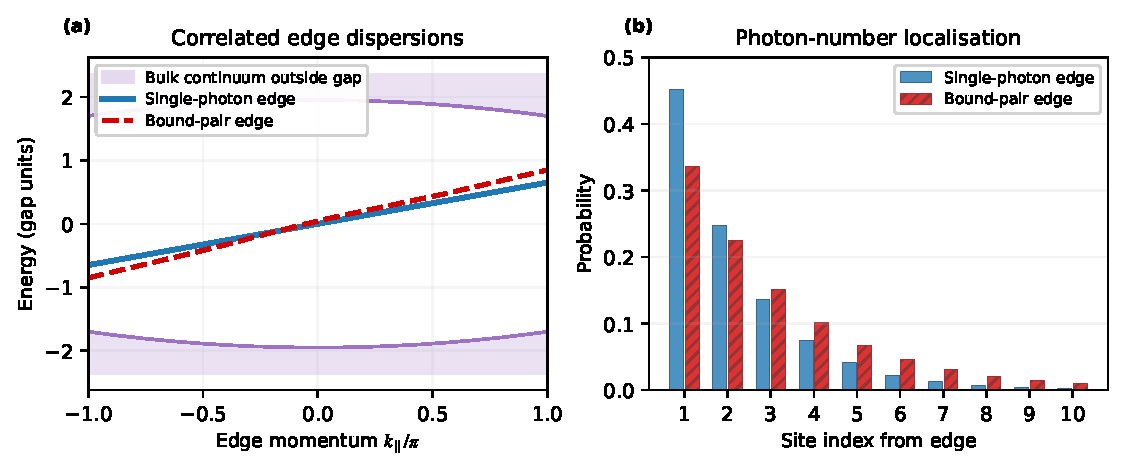
\includegraphics[width=0.92\textwidth]{figures/fig_ch18_quantum_edge_step199.pdf}
  \caption{Quantum topological edge states for correlated photons.
  \textbf{(a)}~Edge dispersions in a topological photonic lattice with
  on-site Kerr interaction.  Single-photon edge modes (solid blue)
  cross the gap linearly; bound photon pairs (dashed red) acquire an
  interaction-shifted dispersion with a slightly different slope,
  reflecting the two-photon binding energy.  The shaded purple regions
  mark the two-photon bulk continuum outside the gap.
  \textbf{(b)}~Site-resolved probability distribution for a single
  photon (blue bars) and a bound pair (red bars) localised at the
  topological edge.  Both states decay exponentially into the bulk,
  but the bound pair has a longer localisation length due to its
  enhanced effective mass.  The panels illustrate that both
  single-photon and bound-pair states can occupy topologically
  protected edge channels; quantitative robustness to disorder requires
  transport or correlation measurements as discussed in the text.}
  \label{fig:ch18-quantum-edge}
\end{figure}


\subsection{Topological protection of quantum coherence}
\label{sec:ch18-coherence-protection}

A fundamental question in quantum topological photonics is whether
the topological protection extends beyond intensity transport to
preserve quantum coherence.  Theoretical analyses show that the
suppression of backscattering in topological edge modes also
suppresses the dephasing caused by elastic scattering from disorder
\cite{ozawa2018topological}.

For a single photon propagating along a topological edge channel
of length $L$, the coherence length is limited by inelastic
processes (absorption, radiation loss) rather than by elastic
scattering.  In a high-quality silicon photonic crystal with
propagation loss $\alpha\sim 1\;\mathrm{dB/cm}$, the coherence
length can exceed $10\;\mathrm{cm}$---far longer than typical
on-chip quantum photonic circuits.

This advantage becomes particularly significant for multi-photon
quantum states, where the sensitivity to decoherence scales with
the number of photons.  Topological protection effectively removes
one of the dominant decoherence channels (elastic backscattering),
leaving only the intrinsic material absorption as the limiting
factor \cite{price2022roadmap}.

\subsection{Outlook: strongly correlated topological photons}
\label{sec:ch18-strongly-correlated}

The ultimate frontier of quantum topological photonics is the regime
of strong photon--photon interactions, where the photonic system can
exhibit analogues of fractional quantum Hall states.  Achieving this
regime requires both a topological band structure and an effective
photon--photon interaction strength comparable to the bandwidth.

Promising platforms include circuit QED lattices, where
superconducting qubits provide strong nonlinearities at microwave
frequencies, and Rydberg--polariton systems, where the long-range
interaction between Rydberg atoms mediates effective photon--photon
interactions at optical frequencies
\cite{ozawa2018topological,price2022roadmap}.

The realisation of fractional topological photonic states would
represent a qualitative advance, enabling the preparation and
manipulation of topologically ordered quantum states of light for
fault-tolerant quantum computation and quantum simulation.

\begin{figure}[t]
  \centering
  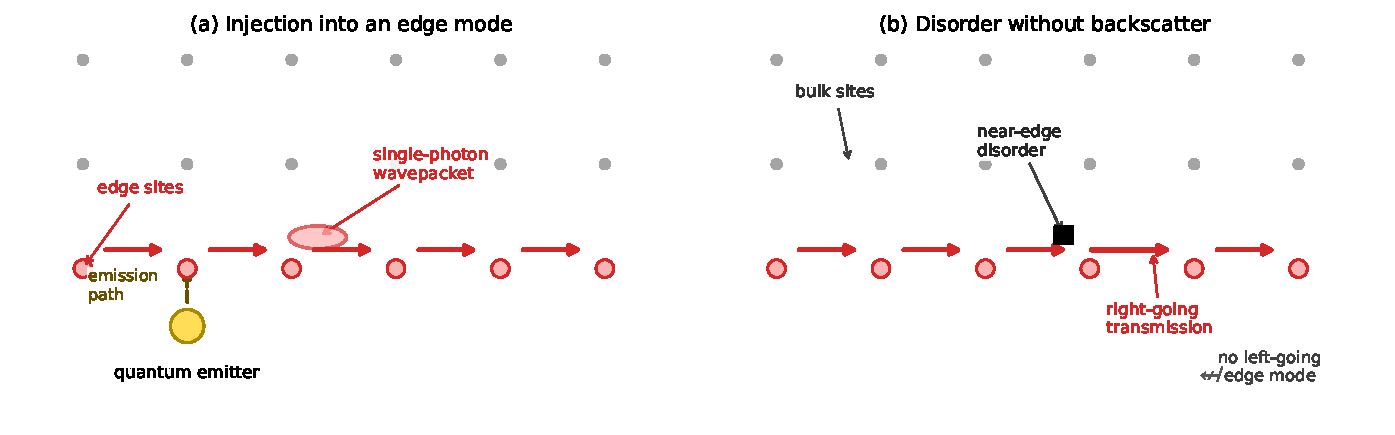
\includegraphics[width=0.86\textwidth]{figures/fig_ch18_quantum_edge_channel.pdf}
  \caption{A quantum emitter coupled to a topological edge channel can launch
  single photons into a protected boundary mode.  The same one-way transport
  principle that suppresses classical backscattering also protects the path
  of quantum optical states against elastic disorder.}
  \label{fig:ch18-quantum-edge-channel}
\end{figure}

The interplay between binding energy and localisation length is
made explicit in Figure~\ref{fig:ch18-bound-pair-binding-log}.

\begin{figure}[t]
  \centering
  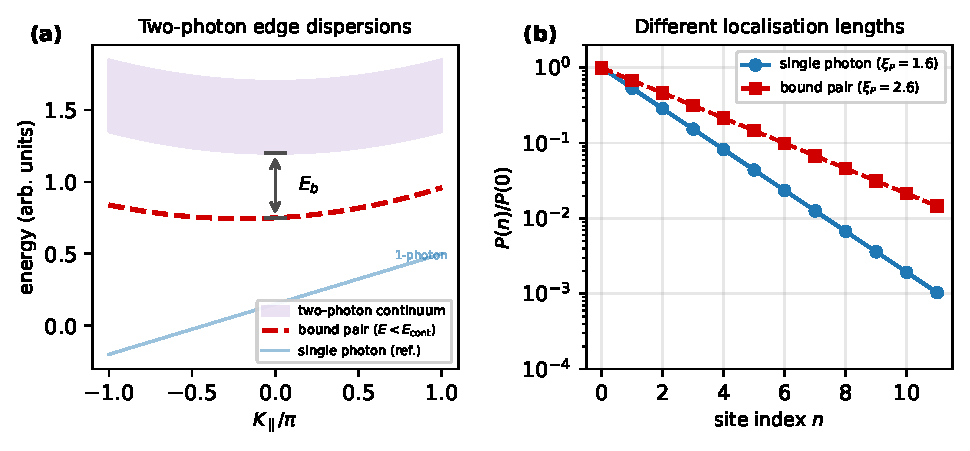
\includegraphics[width=0.92\textwidth]{figures/fig_ch18_bound_pair_binding_log_step236.pdf}
  \caption{Binding energy and localisation of a two-photon
  bound-pair edge state.  \textbf{(a)}~Two-photon edge
  dispersions (schematic): the shaded purple region is the
  two-photon bulk continuum, and the red dashed curve is the
  bound-pair branch lying below the continuum by the binding
  energy $E_b$.  The faint blue line shows the single-photon
  edge mode for reference; it belongs to a different particle-number
  sector and should not be compared directly with $E_b$.
  Energy is in arbitrary units.  \textbf{(b)}~Semilog probability
  profiles at the topological edge: the single-photon state
  (circles) decays as $P(n)/P(0)=\exp(-n/\xi_P)$ with
  $\xi_P=1.6$ sites, while the bound pair (squares) has a
  longer probability localisation length $\xi_P=2.6$ sites
  due to its enhanced effective mass.  Parameters are
  illustrative; actual values depend on the interaction
  strength and lattice geometry.}
  \label{fig:ch18-bound-pair-binding-log}
\end{figure}

\section{Nonlinear topological solitons in Floquet systems}
\label{sec:ch18-floquet-solitons}

The Floquet photonic topological insulators of Chapter~\ref{ch:floquet}
provide a natural arena for topological solitons, because the helical
waveguide arrays that realise Floquet bands are fabricated in glass
substrates with an intrinsic Kerr nonlinearity.

\subsection{Anomalous Floquet solitons}
\label{sec:ch18-anomalous-soliton}

Recall from Section~\ref{sec:ch13-anomalous} that the anomalous
Floquet insulator possesses chiral edge modes in \emph{every}
quasi-energy gap, even though all bulk bands have zero Chern number.
Because these edge modes span the entire quasi-energy Brillouin zone
$[-\pi/T,\pi/T]$, their dispersion is approximately linear over a
wide bandwidth, producing low group-velocity dispersion $D$.  This
means that soliton formation requires a proportionally higher
nonlinearity, but also that the resulting solitons can be very short
in duration.

Mukherjee and Rechtsman (2021) observed unidirectional soliton-like
edge states in a nonlinear Floquet topological insulator realised in
a femtosecond-laser-written waveguide array
\cite{mukherjee2021observation}.  The key experimental signatures
were: (i)~self-focusing of the edge-mode intensity profile as the
input power increased, (ii)~preservation of unidirectional propagation
around sharp corners even in the nonlinear regime, and (iii)~power
thresholds consistent with the NLSE prediction $P_{\mathrm{sol}} =
2|D|/(\gamma w)$ using the measured edge-mode parameters.

The robustness of these Floquet solitons is remarkable.  Because the
anomalous edge mode has no backward-propagating counterpart, the
soliton cannot scatter into a counter-propagating mode even when it
encounters a lattice defect.  The topological gap prevents radiation
into bulk modes as long as the nonlinear index change remains smaller
than the gap width.  Numerical simulations show that the soliton
survives disorder levels up to $\sim 10\%$ of the coupling constant
before bulk radiation sets in \cite{shen2023floquet}.

\subsection{Edge solitons in static Chern insulators}
\label{sec:ch18-static-solitons}

Leykam and Chong (2016) predicted theoretically that self-localised
edge solitons can form along the boundary of a static (non-Floquet)
photonic Chern insulator \cite{leykam2016edge}.  The crucial
difference from conventional waveguide solitons is the topological
origin of the edge mode: the number of soliton-carrying channels is
fixed by the bulk Chern number and cannot be changed by surface
modifications.

Their analysis starts from the tight-binding Haldane model with
an on-site Kerr nonlinearity $\gamma|\psi_n|^2\psi_n$ added to each
lattice site.  For the chiral edge mode of the Chern insulator,
the continuum limit of the discrete NLSE reduces to
Eq.~\eqref{eq:ch18-nlse} with $D$ determined by the edge-mode
curvature and $\gamma$ by the on-site nonlinearity.

The topological protection of these edge solitons degrades gracefully:
at moderate nonlinearity, the soliton propagates with minimal
radiation loss; at strong nonlinearity ($\gamma|\psi|^2 \gtrsim
0.3\,\Delta\omega$), the soliton begins to shed radiation into
the bulk, and eventually a self-induced topological transition can
occur \cite{szameit2020nonlinearity}.

\subsection{Nonlinearity-induced topological transitions}
\label{sec:ch18-nl-transition}

Maczewsky et al.\ (2020) demonstrated experimentally that the Kerr
nonlinearity can itself drive a topological phase transition
\cite{szameit2020nonlinearity}.  In their experiment, a trivial
(topologically trivial) photonic lattice became a topological
insulator when illuminated with sufficiently intense light.  The
mechanism is that the nonlinear index change $\delta n = n_2 |E|^2$
selectively modifies the coupling constants between lattice sites,
effectively changing the parameter that controls the topological
phase.

This observation opens the door to all-optical switching of
topological edge transport: a control beam can turn edge conduction
on or off by crossing the nonlinear topological phase boundary.
The switching speed is limited by the Kerr response time (femtoseconds
in glass, picoseconds in semiconductors), making this a potentially
ultrafast mechanism \cite{chen2025nonlinear}.

\section{Higher-order topological states and nonlinearity}
\label{sec:ch18-hoti-nonlinear}

The intersection of higher-order topology and nonlinearity is an
active frontier.  In a second-order topological insulator (SOTI), the
protected states are zero-dimensional corner modes rather than
one-dimensional edge modes.  These corner modes are tightly confined
in all directions, producing extremely small mode volumes and
correspondingly large nonlinear coefficients $\gamma \propto
1/A_{\mathrm{eff}}$.

Kartashov (2024) predicted the existence of topological corner
solitons in a SOTI created by twisting the unit cell of a photonic
lattice \cite{kartashov2024solitons}.  The corner solitons are
pinned to specific lattice corners by topology and stabilised
against collapse by the discrete lattice structure.  Their power
threshold is orders of magnitude lower than for bulk solitons because
of the extreme field confinement at the corner.

Extending to quadratic ($\chi^{(2)}$) nonlinearity, Kartashov (2025)
showed that parametric down-conversion in a SOTI can generate
entangled photon pairs that are topologically confined to lattice
corners \cite{kartashov2025quadratic}.  This suggests a route to
combining the robustness of topological protection with the quantum
correlations needed for photonic quantum information processing.

\section{Outlook: open problems at the nonlinear--quantum frontier}
\label{sec:ch18-frontier-outlook}

The nonlinear and quantum extensions of topological photonics raise
several deep open questions that connect to fundamental physics.

The first is the \emph{many-body gap problem}: in a strongly
interacting photonic system (e.g.\ circuit QED at large $U/J$), does
the many-body energy gap inherit the robustness of the single-particle
topological gap?  Mean-field studies suggest yes for weak interactions,
but the strongly correlated regime---where fractional Chern insulator
states are predicted---remains largely unexplored experimentally
\cite{ozawa2018topological}.

The second is the \emph{measurement problem}: photonic systems are
inherently open (photons leak out of cavities and waveguides), and
quantum measurements in topological photonic systems typically involve
detecting photons that have left the system.  How does the interplay
between topology, non-Hermiticity (from loss), and quantum measurement
affect the topological protection of quantum states?  Recent work on
non-Hermitian topology (Chapter~\ref{ch:non-hermitian}) provides a
framework, but the full quantum treatment remains an open challenge
\cite{wang2021topological,ding2022non}.

The third is the \emph{scaling problem}: demonstrating fractional
topological photonic states requires lattices with hundreds of sites,
strong and uniform photon--photon interactions, and sub-microsecond
measurement cycles.  Current circuit QED technology is approaching
these requirements, but significant engineering advances are still
needed.  Alternative platforms---such as Rydberg polaritons in
photonic crystal slabs or exciton--polariton lattices---may offer
complementary routes \cite{price2022roadmap}.

\section*{Exercises}

\begin{exercise}
  Show that the nonlinear Schr\"odinger equation
  \eqref{eq:ch18-nlse} (in the co-moving frame, with $v_g=0$) admits
  the soliton solution \eqref{eq:ch18-soliton}, and find $A$, $w$,
  and $\beta$ in terms of $D$ and $\gamma$.
\end{exercise}

\begin{exercise}
  Estimate the threshold intensity for a self-induced topological
  transition in a silicon photonic crystal ($n_2\approx
  4.5\times 10^{-18}\;\mathrm{m}^2/\mathrm{W}$,
  $\Delta\omega/\omega\approx 2\%$, $\omega/(2\pi)\approx
  193\;\mathrm{THz}$).  Is this achievable with current ultrafast
  laser technology?
\end{exercise}

\begin{exercise}
  For a topological laser with edge-mode group velocity $v_g=c/30$,
  round-trip length $L=200\;\mu\mathrm{m}$, and material gain
  $g_0=100\;\mathrm{cm}^{-1}$, estimate the lasing threshold using
  equation \eqref{eq:ch18-threshold}.  Assume negligible absorption
  and a residual reflectivity $R=10^{-3}$.
\end{exercise}

\begin{exercise}
  In a coupled-cavity array with on-site Kerr nonlinearity $U$ and
  hopping $J$, the mean-field phase diagram includes a superfluid
  phase (for $U/J\ll 1$) and a Mott-insulator phase (for $U/J\gg 1$).
  When the hopping carries a synthetic magnetic flux, describe
  qualitatively what happens to the Mott insulator at integer filling
  in a Chern band.
\end{exercise}

\begin{exercise}
  A Hong-Ou-Mandel experiment is performed with two indistinguishable
  photons injected into a topological edge mode and a trivial waveguide
  mode, respectively.  Describe how the two-photon coincidence rate
  depends on the time delay and the topological protection.
\end{exercise}


% ======================================================================
\appendix
\part*{Appendices}
\addcontentsline{toc}{part}{Appendices}

\chapter{Vector Identities and Functional Analysis}
\label{app:vector-identities}
% ======================================================================
%  Appendix A — Vector Identities and Functional Analysis  (EXPANDED)
% ======================================================================

\section{Vector calculus identities}
\label{sec:appA-vector}

\subsection{Fundamental differential identities}
\label{sec:appA-differential}

The following identities are used throughout the derivations of
Chapters~2--5.  All fields are assumed sufficiently smooth.

For any scalar field $\phi$ and vector fields $\mathbf{F}$,
$\mathbf{G}$:
\begin{align}
  \nabla\times(\nabla\phi) &= \mathbf{0}\,,
    \label{eq:appA-curl-grad}\\
  \nabla\cdot(\nabla\times\mathbf{F}) &= 0\,,
    \label{eq:appA-div-curl}\\
  \nabla\times(\nabla\times\mathbf{F})
    &= \nabla(\nabla\cdot\mathbf{F})-\nabla^2\mathbf{F}\,,
    \label{eq:appA-curl-curl}\\
  \nabla\cdot(\phi\mathbf{F})
    &= \phi\,\nabla\cdot\mathbf{F}
    +\mathbf{F}\cdot\nabla\phi\,,
    \label{eq:appA-div-product}\\
  \nabla\times(\phi\mathbf{F})
    &= \phi\,\nabla\times\mathbf{F}
    +(\nabla\phi)\times\mathbf{F}\,.
    \label{eq:appA-curl-product}
\end{align}
The double-curl identity \eqref{eq:appA-curl-curl} is especially
important: it converts the Maxwell wave equation into a Helmholtz
equation for a divergence-free field.

For products of two vector fields:
\begin{align}
  \nabla\cdot(\mathbf{F}\times\mathbf{G})
    &= \mathbf{G}\cdot(\nabla\times\mathbf{F})
    -\mathbf{F}\cdot(\nabla\times\mathbf{G})\,,
    \label{eq:appA-div-cross}\\
  \nabla(\mathbf{F}\cdot\mathbf{G})
    &= (\mathbf{F}\cdot\nabla)\mathbf{G}
    +(\mathbf{G}\cdot\nabla)\mathbf{F}
    +\mathbf{F}\times(\nabla\times\mathbf{G})
    +\mathbf{G}\times(\nabla\times\mathbf{F})\,.
    \label{eq:appA-grad-dot}
\end{align}

\subsection{Integral theorems}
\label{sec:appA-integral}

The divergence (Gauss) theorem:
\begin{equation}\label{eq:appA-gauss}
  \int_V\nabla\cdot\mathbf{F}\,\dd^3r
  = \oint_{\partial V}\mathbf{F}\cdot\hat{n}\,\dd S\,.
\end{equation}
The curl (Stokes) theorem:
\begin{equation}\label{eq:appA-stokes}
  \int_S(\nabla\times\mathbf{F})\cdot\hat{n}\,\dd S
  = \oint_{\partial S}\mathbf{F}\cdot\dd\boldsymbol{\ell}\,.
\end{equation}
These are used in the Poynting-theorem derivation
(\secref{sec:ch2-poynting}) and in the self-adjointness proof for
the Maxwell curl operator (\secref{sec:ch3-self-adjoint})
\cite{press2026photonic}.

\subsection{The Levi-Civita symbol and cross products}
\label{sec:appA-levi-civita}

The Levi-Civita symbol $\epsilon_{ijk}$ is defined by $\epsilon_{123}=1$
and antisymmetry under transposition of any two indices.  Cross products
and curls are expressed as
\begin{equation}\label{eq:appA-cross}
  (\mathbf{A}\times\mathbf{B})_i
  = \sum_{jk}\epsilon_{ijk}A_j B_k\,,
  \qquad
  (\nabla\times\mathbf{F})_i
  = \sum_{jk}\epsilon_{ijk}\partial_j F_k\,.
\end{equation}
The contracted product identity is
\begin{equation}\label{eq:appA-eps-contract}
  \sum_k\epsilon_{ijk}\epsilon_{klm}
  = \delta_{il}\delta_{jm}-\delta_{im}\delta_{jl}\,,
\end{equation}
from which many vector identities follow algebraically.

\section{The Maxwell integration-by-parts lemma}
\label{sec:appA-ibp}

\subsection{Statement}
\label{sec:appA-ibp-statement}

The central analytic tool in Chapters~2--3 is the integration-by-parts
identity for the six-component Maxwell curl operator $\Maxop$.

\begin{proposition}[Maxwell integration by parts]
\label{prop:appA-ibp}
For six-component fields $\emfield_1=(\Efield_1,\Hfield_1)^T$ and
$\emfield_2=(\Efield_2,\Hfield_2)^T$ on a domain $\Omega$ with
boundary $\partial\Omega$:
\begin{equation}\label{eq:appA-ibp}
  \int_\Omega\emfield_1^\dagger\,\Maxop\,\emfield_2\,\dd^3r
  - \int_\Omega(\Maxop\,\emfield_1)^\dagger\,\emfield_2\,\dd^3r
  = \oint_{\partial\Omega}\bigl[
    (\hat{n}\times\Efield_1^*)^T\Hfield_2
    - (\hat{n}\times\Hfield_1^*)^T\Efield_2
  \bigr]\,\dd S\,.
\end{equation}
\end{proposition}

The identity is more than a vector-calculus convenience.  It says that
self-adjointness of Maxwell's curl block is decided at the boundary,
not in the bulk algebra alone.  Figure~\ref{fig:appA-ibp-boundary}
shows this logic: the volume commutator of the curl operator is
converted into tangential electric and magnetic traces on
$\partial\Omega$.  Periodic boundary conditions, perfectly conducting
walls, or decay at infinity remove this boundary pairing; an interface
problem keeps it, and that surviving term is the analytic shadow of an
edge channel.

\begin{figure}[t]
  \centering
  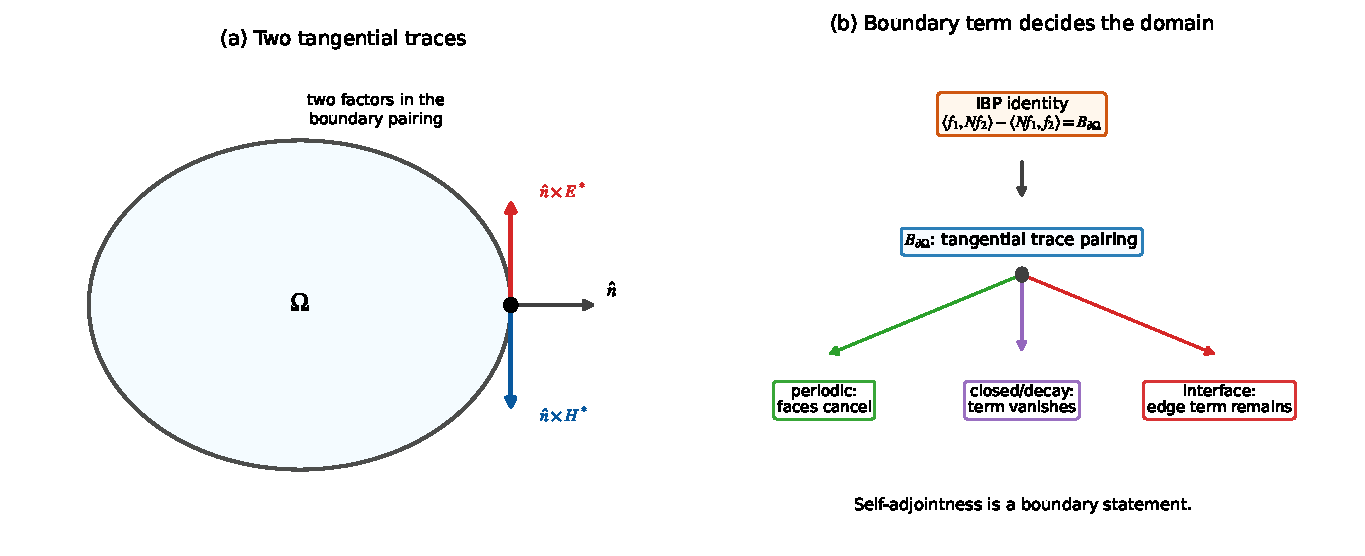
\includegraphics[width=0.94\textwidth]{figures/fig_appA_ibp_boundary.pdf}
  \caption{The Maxwell integration-by-parts identity as a boundary
  statement.  The difference between the two curl-block matrix elements
  is a surface pairing of tangential field traces.  When opposite
  faces cancel, fields decay, or boundary conditions set the trace
  pairing to zero, the Maxwell curl block becomes symmetric on the
  chosen domain.  At an interface the same boundary term is the place
  where edge-mode physics enters the operator proof.}
  \label{fig:appA-ibp-boundary}
\end{figure}


\subsection{Derivation}
\label{sec:appA-ibp-proof}

We start from the divergence identity \eqref{eq:appA-div-cross}:
\begin{equation}
  \nabla\cdot(\Efield_1^*\times\Hfield_2)
  = \Hfield_2\cdot(\nabla\times\Efield_1^*)
  - \Efield_1^*\cdot(\nabla\times\Hfield_2)\,.
\end{equation}
Similarly:
\begin{equation}
  \nabla\cdot(\Hfield_1^*\times\Efield_2)
  = \Efield_2\cdot(\nabla\times\Hfield_1^*)
  - \Hfield_1^*\cdot(\nabla\times\Efield_2)\,.
\end{equation}
Adding these two expressions and rearranging in terms of the
six-component operator $\Maxop$ gives \eqref{eq:appA-ibp}.  Applying
the divergence theorem converts the divergence terms into the surface
integral over $\partial\Omega$.

When the boundary term vanishes (e.g.\ for periodic boundary conditions,
perfectly conducting walls, or fields that decay at infinity), the
curl operator $\Maxop$ is formally self-adjoint under the bare $L^2$
inner product.  The physical self-adjointness under the energy inner
product $\langle\cdot|\Mmat|\cdot\rangle$ follows from
$\Maxop^\dagger=\Maxop$ combined with $\Mmat=\Mmat^\dagger$
(lossless medium).

\section{Spectral theory of self-adjoint operators}
\label{sec:appA-spectral}

\subsection{Finite-dimensional review}
\label{sec:appA-finite}

For a finite-dimensional Hermitian matrix $H=H^\dagger$ acting on \cite{raman2010photonic}
$\mathbb{C}^N$, the spectral theorem guarantees real eigenvalues
$\lambda_1\leq\cdots\leq\lambda_N$, a complete orthonormal basis of
eigenvectors $|v_n\rangle$, and the resolution of the identity:
\begin{equation}\label{eq:appA-spectral-finite}
  H = \sum_{n=1}^N\lambda_n\,|v_n\rangle\langle v_n|\,,
  \qquad
  \mathbf{I} = \sum_{n=1}^N|v_n\rangle\langle v_n|\,.
\end{equation}

\subsection{Extension to the Maxwell operator}
\label{sec:appA-maxwell-spectral}

The Maxwell eigenvalue problem
$\Maxop\emfield=\omega\Mmat\emfield$ on a bounded or periodic
domain, with appropriate boundary conditions, is a generalised
eigenvalue problem with a positive-definite ``weight'' $\Mmat$.  The
key spectral properties are:

All eigenfrequencies $\omega_n$ are real, because the operator
$\Mmat^{-1}\Maxop$ is self-adjoint with respect to the
$\Mmat$-weighted inner product.

The eigenmodes $\emfield_n$ are orthogonal under the energy inner
product: $\emip{\emfield_m}{\emfield_n}=\delta_{mn}$ after
normalisation.

The eigenmodes form a complete set: any sufficiently smooth field
satisfying the boundary conditions can be expanded in the eigenmode
basis.

For a periodic medium (photonic crystal), the eigenvalue problem
decomposes into a family of problems parametrised by the Bloch
wavevector $\kvec$, each of which has a discrete spectrum
$\{\omega_{n\kvec}\}_{n=1}^\infty$.  As $\kvec$ varies over the
Brillouin zone, these eigenvalues trace the photonic band structure.

\subsection{The min-max principle}
\label{sec:appA-minmax}

The min-max (Courant--Fischer) characterisation of eigenvalues
provides variational bounds:
\begin{equation}\label{eq:appA-minmax}
  \omega_n^2 = \min_{\dim V=n}\max_{\emfield\in V\backslash\{0\}}
  \frac{\langle\emfield|\Maxop^2|\emfield\rangle}
  {\emip{\emfield}{\emfield}}\,.
\end{equation}
This is the electromagnetic analog of the Rayleigh--Ritz variational
principle in quantum mechanics \cite{nittis2020equivalence}.  It is used in perturbation theory
to bound the frequency shifts caused by material changes \cite{atala2013direct}.

\section{Perturbation theory for the Maxwell eigenproblem}
\label{sec:appA-perturbation}

\subsection{Non-degenerate perturbation theory}
\label{sec:appA-nondegenerate}

Consider a perturbation $\Mmat\to\Mmat+\delta\Mmat$ of the material
matrix.  The first-order frequency shift of a non-degenerate mode
$\emfield_n$ is
\begin{equation}\label{eq:appA-first-order}
  \delta\omega_n
  = -\frac{\omega_n}{2}\,
  \frac{\langle\emfield_n|\delta\Mmat|\emfield_n\rangle}
  {\emip{\emfield_n}{\emfield_n}}\,.
\end{equation}
This is the electromagnetic Hellmann--Feynman theorem; it appears in
Equation~\eqref{eq:ch4-hellmann-feynman} and is used extensively in Chapters~7
and~11.

\subsection{Degenerate perturbation theory}
\label{sec:appA-degenerate}

When two or more modes are degenerate at $\omega_0$, the first-order
correction is found by diagonalising the perturbation within the
degenerate subspace.  Let $\{|\emfield_\alpha\rangle\}_{\alpha=1}^p$
be the degenerate modes.  The first-order frequency splittings are the
eigenvalues of the $p\times p$ matrix:
\begin{equation}\label{eq:appA-degenerate}
  V_{\alpha\beta}
  = -\frac{\omega_0}{2}\,
  \frac{\langle\emfield_\alpha|\delta\Mmat|\emfield_\beta\rangle}
  {\emip{\emfield_\alpha}{\emfield_\alpha}}\,.
\end{equation}
This is the key formula for deriving the effective Dirac Hamiltonian
at high-symmetry points (Chapter~6) and the mass terms from
time-reversal or inversion breaking (Chapters~7, 11, 12).

\section{Function spaces and boundary conditions}
\label{sec:appA-function-spaces}

\subsection{The relevant Sobolev spaces} \cite{initio2026pdf}
\label{sec:appA-sobolev}

The natural function space for the Maxwell eigenvalue problem is the
space of square-integrable vector fields with square-integrable curl:
\begin{equation}\label{eq:appA-hcurl}
  H(\mathrm{curl},\Omega)
  = \bigl\{\mathbf{F}\in L^2(\Omega)^3
  \;\big|\;\nabla\times\mathbf{F}\in L^2(\Omega)^3\bigr\}\,.
\end{equation}
This is the electromagnetic analog of the Sobolev space $H^1$.  The
boundary conditions (perfect conductor, periodic, or radiation) are
imposed by restricting to appropriate subspaces.

For periodic media (photonic crystals), the relevant space is the
Bloch-periodic version:
\begin{equation}\label{eq:appA-bloch-space}
  H_\kvec(\mathrm{curl},\Omega_{\mathrm{cell}})
  = \bigl\{\mathbf{F}\in H(\mathrm{curl},\Omega_{\mathrm{cell}})
  \;\big|\;
  \mathbf{F}(\rvec+\avec)=\ee^{\ii\kvec\cdot\avec}\mathbf{F}(\rvec)
  \;\forall\;\avec\in\Lambda\bigr\}\,,
\end{equation}
where $\Lambda$ is the Bravais lattice.

\subsection{Completeness and regularity}
\label{sec:appA-completeness}

For a lossless medium with positive-definite $\Mmat$, the Maxwell
eigenproblem on a bounded domain (or on a unit cell with Bloch boundary
conditions) has a discrete spectrum accumulating at infinity.  The
eigenmodes form a complete orthonormal basis in the $\Mmat$-weighted
$L^2$ space.

For smooth material parameters ($\Mmat\in C^\infty$), the eigenmodes
are themselves smooth inside the domain.  At material interfaces where
$\Mmat$ has jump discontinuities, the tangential components of
$\Efield$ and $\Hfield$ remain continuous, but normal components may
have jumps proportional to the contrast.

\section{Useful matrix identities}
\label{sec:appA-matrix}

For $2\times 2$ matrices expressed in terms of Pauli matrices,
$H=d_0\mathbf{I}+\mathbf{d}\cdot\boldsymbol{\sigma}$:
\begin{align}
  \det(H) &= d_0^2 - |\mathbf{d}|^2\,,\\
  \Tr(H) &= 2d_0\,,\\
  H^{-1} &= \frac{d_0\mathbf{I}-\mathbf{d}\cdot\boldsymbol{\sigma}}
  {d_0^2-|\mathbf{d}|^2}\,,\\
  \ee^{\ii\theta\,\hat{n}\cdot\boldsymbol{\sigma}}
  &= \cos\theta\,\mathbf{I}+\ii\sin\theta\,
  \hat{n}\cdot\boldsymbol{\sigma}\,.
\end{align}
The Pauli-matrix trace identities are:
\begin{align}
  \Tr(\sigma_a) &= 0\,,\\
  \Tr(\sigma_a\sigma_b) &= 2\delta_{ab}\,,\\
  \Tr(\sigma_a\sigma_b\sigma_c) &= 2\ii\epsilon_{abc}\,.
\end{align}
These identities are used extensively in the effective-Hamiltonian
derivations of Chapters~6--8, 11--12, and 15.

\section{The Baker--Campbell--Hausdorff formula}
\label{sec:appA-bch}

For operators $A$ and $B$:
\begin{equation}\label{eq:appA-bch}
  \ee^A\ee^B = \exp\Bigl(A+B+\frac{1}{2}[A,B]
  +\frac{1}{12}\bigl([A,[A,B]]+[B,[B,A]]\bigr)+\cdots\Bigr)\,.
\end{equation}
This is used in the derivation of the Wilson loop
(\secref{sec:ch5-wilson}) and in the analysis of Floquet evolution
operators (Chapter~\ref{ch:floquet}).

\section{The electromagnetic Green's function}
\label{sec:appA-green}

\subsection{Definition and properties}
\label{sec:appA-green-def}

The Green's function (resolvent kernel) of the Maxwell operator is
defined by
\begin{equation}\label{eq:appA-green-def}
  \bigl(\Maxop - \omega\,\Mmat\bigr)\,
  \mathbf{G}(\rvec,\rvec';\omega)
  = \delta^{(3)}(\rvec-\rvec')\,\mathbf{I}_6\,,
\end{equation}
where $\mathbf{I}_6$ is the $6\times 6$ identity.  Formally, the
Green's function is the kernel of the resolvent operator
$R(\omega)=(\Maxop-\omega\Mmat)^{-1}$:
\begin{equation}\label{eq:appA-resolvent}
  R(\omega) = \sum_n
  \frac{|\emfield_n\rangle\langle\emfield_n|\Mmat}
  {\omega_n-\omega}\,,
\end{equation}
where the sum runs over the complete set of eigenmodes.  The poles of
$R(\omega)$ are the eigenfrequencies $\omega_n$, and the residue at
each pole projects onto the corresponding eigenmode.

\subsection{Spectral representation in periodic media}
\label{sec:appA-green-periodic}

For a photonic crystal, the Green's function decomposes over Bloch
wavevectors:
\begin{equation}\label{eq:appA-green-bloch}
  \mathbf{G}(\rvec,\rvec';\omega)
  = \sum_n\int_{\mathrm{BZ}}\frac{\dd^d k}{(2\pi)^d}
  \frac{\emfield_{n\kvec}(\rvec)\,
  \emfield_{n\kvec}^\dagger(\rvec')\,\Mmat}
  {\omega_{n\kvec}-\omega}\,.
\end{equation}
The imaginary part $\imag\,\Tr\,\mathbf{G}(\rvec,\rvec;\omega+\ii 0^+)$
gives the local density of states
\cite{ozawa2018topological}:
\begin{equation}\label{eq:appA-ldos}
  \rho(\rvec,\omega)
  = -\frac{1}{\pi}\imag\,\Tr\bigl[\Mmat\,
  \mathbf{G}(\rvec,\rvec;\omega+\ii 0^+)\bigr]\,.
\end{equation}
This relation connects the spectral properties of the Maxwell operator
(through the Green's function poles) to the experimentally observable
local density of states.

\subsection{Gap Chern number from the Green's function}
\label{sec:appA-green-chern}

The Chern number can be expressed directly in terms of the Green's
function, without requiring explicit knowledge of the eigenmodes.
For a frequency $\omega$ lying in a spectral gap, the gap Chern number
is \cite{silveirinha2016bulk}
\begin{equation}\label{eq:appA-chern-green}
  \Chern_{\mathrm{gap}}(\omega)
  = \frac{\epsilon_{ab}}{4\pi\ii}\int_{\mathrm{BZ}}
  \Tr\bigl[
    G\,\partial_{k_a}G^{-1}\,G\,\partial_{k_b}G^{-1}
  \bigr]\,\dd^2 k\,,
\end{equation}
where $G\equiv\mathbf{G}(\kvec;\omega)$ is the $\kvec$-dependent
Green's function evaluated at the gap frequency.  This formula is
especially useful for non-Hermitian and continuum systems where the
eigenmode basis may not be well defined \cite{gangaraj2016berry}.

\section{Tensor product structure of the six-component space}
\label{sec:appA-tensor}

The six-component Maxwell field $\emfield=(\Efield,\Hfield)^T$ lives
in the direct sum $\mathcal{H}=\mathcal{H}_E\oplus\mathcal{H}_H$,
where $\mathcal{H}_E$ and $\mathcal{H}_H$ are the spaces of
square-integrable 3-component electric and magnetic fields
respectively.  The material matrix $\Mmat$ and the curl operator
$\Maxop$ have specific block structures in this decomposition:
\begin{equation}\label{eq:appA-block-M}
  \Mmat = \begin{pmatrix}
    \varepsilon_0\epst & 0 \\ 0 & \mu_0\mut
  \end{pmatrix},
  \qquad
  \Maxop = \begin{pmatrix}
    0 & \nabla\times \\
    -\nabla\times & 0
  \end{pmatrix},
\end{equation}
in the absence of bianisotropy ($\xit=\zetat=0$).  The off-diagonal
structure of $\Maxop$ couples the electric and magnetic sectors, while
the block-diagonal structure of $\Mmat$ separates them.  This
``chiral'' structure is the origin of many symmetry properties:
for example, $\Maxop$ anticommutes with the matrix
$\sigma_3=\mathrm{diag}(\mathbf{I}_3,-\mathbf{I}_3)$, so that
eigenfrequencies come in $\pm\omega$ pairs for lossless media.

When bianisotropic coupling $\xit\neq 0$ is present (as in the
Khanikaev metamaterial of Chapter~\ref{ch:reciprocal-designs}), the
material matrix acquires off-diagonal blocks, and the direct-sum
decomposition breaks down.  The pseudospin topology of
Chapter~\ref{ch:reciprocal-designs} can be understood as a controlled
restoration of this decomposition through the bianisotropic coupling.

\section{Proof of the curl-curl identity}
\label{sec:appA-curl-curl-proof}

The double-curl identity $\nabla\times(\nabla\times\mathbf{F})
=\nabla(\nabla\cdot\mathbf{F})-\nabla^2\mathbf{F}$ is fundamental to
the reduction of the Maxwell wave equation to the Helmholtz equation.
We give a component-wise proof using the Levi-Civita symbol.

\begin{proof}
The $i$-th component of $\nabla\times(\nabla\times\mathbf{F})$ is
\begin{equation}
  [\nabla\times(\nabla\times\mathbf{F})]_i
  = \epsilon_{ijk}\partial_j(\nabla\times\mathbf{F})_k
  = \epsilon_{ijk}\epsilon_{klm}\partial_j\partial_l F_m\,.
\end{equation}
Using the contraction identity $\epsilon_{ijk}\epsilon_{klm}
=\delta_{il}\delta_{jm}-\delta_{im}\delta_{jl}$:
\begin{align}
  [\nabla\times(\nabla\times\mathbf{F})]_i
  &= (\delta_{il}\delta_{jm}-\delta_{im}\delta_{jl})
  \partial_j\partial_l F_m \notag\\
  &= \partial_j\partial_i F_j - \partial_j\partial_j F_i \notag\\
  &= \partial_i(\nabla\cdot\mathbf{F}) - \nabla^2 F_i\,.
\end{align}
This is the $i$-th component of
$\nabla(\nabla\cdot\mathbf{F})-\nabla^2\mathbf{F}$.
\end{proof}

\section{Self-adjoint extensions and boundary conditions}
\label{sec:appA-selfadjoint}

\subsection{The domain of the curl operator}
\label{sec:appA-curl-domain}

The Maxwell curl operator $\Maxop$ is formally defined on smooth,
compactly supported 6-component fields \cite{bernevig2006quantum}.  To make $\Maxop$
self-adjoint in the Hilbert space
$\mathcal{H}=L^2(\Omega;\Mmat\,\dd V)$ (with the electromagnetic
energy inner product), one must specify boundary conditions.

On a domain $\Omega$ with boundary $\partial\Omega$, the natural
boundary condition for the lossless Maxwell problem is the perfect
electric conductor (PEC) condition:
\begin{equation}\label{eq:appA-pec}
  \hat{n}\times\Efield\big|_{\partial\Omega} = 0\,,
\end{equation}
where $\hat{n}$ is the outward unit normal.  With this condition, the
integration-by-parts identity
\begin{equation}\label{eq:appA-ibp-maxwell}
  \emip{\emfield_1}{\Maxop\emfield_2}
  - \emip{\Maxop\emfield_1}{\emfield_2}
  = \oint_{\partial\Omega}
  (\Efield_1\times\Hfield_2-\Efield_2\times\Hfield_1)
  \cdot\hat{n}\,\dd S
\end{equation}
shows that the boundary term vanishes, and $\Maxop$ is symmetric
(formally self-adjoint) on the PEC domain.  A rigorous proof of
essential self-adjointness requires functional-analytic tools
(Friedrichs extension, graph norm estimates), but the key physical
insight is that the boundary conditions determine the domain of
$\Maxop$, and hence the spectrum \cite{gangaraj2016berry}.

\subsection{Boundary conditions and edge modes}
\label{sec:appA-bc-edge}

Different boundary conditions produce different self-adjoint
extensions of $\Maxop$, and hence different spectra.  The topological
edge modes discussed in Chapters~7--9 arise precisely because the
boundary changes the self-adjoint extension: the bulk operator has a
gapped spectrum, but the half-space operator (with PEC or impedance
boundary conditions) has additional eigenvalues in the gap.

The number of these in-gap eigenvalues is determined by the Chern
number of the bulk bands, through the bulk-edge correspondence.  This
is a rigorous mathematical statement: the spectral flow of the
boundary problem equals the Chern number of the bulk problem,
regardless of the specific boundary condition chosen
\cite{silveirinha2016bulk,ozawa2018topological}.

\section{Spectral theory of the Maxwell operator}
\label{sec:appA-spectral-theory}

\subsection{Essential and discrete spectrum}
\label{sec:appA-essential-discrete}

The spectrum of $\Maxop$ in a periodic medium decomposes into two
parts.  The \emph{essential spectrum} consists of the photonic bands:
continuous intervals of $\omega$ filled by propagating Bloch modes.
The \emph{discrete spectrum} consists of isolated eigenvalues
(localised defect modes or edge modes), which can appear in band gaps.

For a perfect photonic crystal (no defects, no boundaries), the
spectrum is purely essential and consists of the union of all photonic
bands.  When a boundary or defect is introduced, discrete eigenvalues
may appear in the gaps.  The topological edge modes are precisely such
discrete eigenvalues, whose existence is guaranteed by the nonzero
Chern number of the bulk bands.

\subsection{Weyl's theorem and stability of the essential spectrum}
\label{sec:appA-weyl}

Weyl's theorem states that the essential spectrum of a self-adjoint
operator is invariant under compact perturbations.  In the photonic
context, this means that local defects (finite-range changes in the
material matrix $\Mmat$) cannot change the band structure of the bulk
crystal; they can only add or remove discrete eigenvalues in the gaps.

This stability is the mathematical foundation of topological
protection: the bulk gap cannot be closed by any local perturbation,
so the edge modes that are topologically required to exist in the gap
are also protected against local perturbations
\cite{ozawa2018topological}.

\section{Bloch decomposition and direct integral}
\label{sec:appA-bloch-decomposition}

For a photonic crystal with lattice $\Lambda$, the Hilbert space
decomposes as a direct integral over the Brillouin zone:
\begin{equation}\label{eq:appA-direct-integral}
  \mathcal{H}
  = \int_{\mathrm{BZ}}^\oplus\mathcal{H}_\kvec\,\frac{\dd^d k}{(2\pi)^d}\,,
\end{equation}
where $\mathcal{H}_\kvec=L^2(\Omega_{\mathrm{cell}};\Mmat\,\dd V)$
is the Hilbert space of cell-periodic fields at fixed $\kvec$.  The
Maxwell operator decomposes correspondingly:
$\Maxop=\int_{\mathrm{BZ}}^\oplus\Maxop(\kvec)\,\dd^d k/(2\pi)^d$.

Each fibre operator $\Maxop(\kvec)$ acts on the compact domain
$\Omega_{\mathrm{cell}}$ with periodic boundary conditions, and
therefore has a purely discrete spectrum:
$\omega_{1,\kvec}\leq\omega_{2,\kvec}\leq\cdots$.  The union of
these discrete spectra over all $\kvec$ gives the photonic bands,
which form the essential spectrum of the full operator.  The
eigenmodes $\mathbf{u}_{n\kvec}$ provide the Bloch basis used
throughout this book \cite{gangaraj2016berry,silveirinha2016bulk}.

\section{Minimax characterisation of eigenvalues}
\label{sec:appA-minimax}

The eigenfrequencies of the cell-periodic Maxwell operator can be
characterised by a minimax (Courant--Fischer) principle.  For the
$n$-th eigenvalue:
\begin{equation}\label{eq:appA-minimax}
  \omega_n^2 = \min_{\dim V=n}\,
  \max_{\emfield\in V,\;\emfield\neq 0}\,
  \frac{\eip{\emfield}{\Maxop^2\emfield}}
  {\eip{\emfield}{\Mmat^2\emfield}}\,,
\end{equation}
where the minimum is over all $n$-dimensional subspaces $V$ of the
domain of $\Maxop$.  This variational characterisation has two
important consequences.

First, it implies that the eigenfrequencies are monotonically ordered:
$\omega_1\leq\omega_2\leq\cdots$.  Second, it provides bounds on how
the eigenfrequencies change under perturbations of the material matrix:
if $\Mmat$ is replaced by $\Mmat+\delta\Mmat$ with
$\|\delta\Mmat\|\leq\eta\|\Mmat\|$, then the eigenfrequencies shift
by at most $O(\eta)$.  This is the mathematical basis for the
stability of the photonic band structure under weak disorder
\cite{ozawa2018topological}.

\section{Perturbation bounds for photonic band gaps}
\label{sec:appA-perturbation-gaps}

\subsection{First-order perturbation of eigenfrequencies}
\label{sec:appA-first-order-pert}

For a small perturbation $\Mmat\to\Mmat+\delta\Mmat$ of the material
matrix, the first-order shift of the $n$-th eigenfrequency is
\begin{equation}\label{eq:appA-first-order-shift}
  \delta\omega_n = -\frac{\omega_n}{2}\,
  \frac{\eip{\mathbf{u}_n}{\delta\Mmat\,\mathbf{u}_n}}
  {\eip{\mathbf{u}_n}{\Mmat\,\mathbf{u}_n}}\,.
\end{equation}
This formula, which follows from the Hellmann--Feynman theorem applied
to the generalised eigenvalue problem
$\Maxop\mathbf{u}=\omega\Mmat\mathbf{u}$, shows that the frequency
shift is proportional to the overlap of the mode with the perturbation,
weighted by the energy inner product.

For a gyrotropic perturbation $\delta\Mmat=\ii\kappa_\mu\sigma_y$
(Faraday rotation), the first-order shift vanishes for modes with
definite symmetry under time reversal, and the gap opening occurs at
second order---consistent with the discussion in
Chapter~\ref{ch:breaking-tr}.

\subsection{Gap stability under disorder}
\label{sec:appA-gap-stability}

The band gap survives under disorder as long as the perturbation
strength is smaller than the gap width:
$\|\delta\Mmat\|<\Delta\omega/\omega_{\mathrm{mid}}$.  This can be
made rigorous using the minimax principle: any perturbation that
shifts the $n$-th eigenvalue by less than $\Delta\omega/2$ cannot
close the gap between bands $n$ and $n+1$.  This provides a
quantitative criterion for the robustness of photonic topological
protection \cite{price2022roadmap}.


\section{Sobolev spaces and regularity of Maxwell solutions}
\label{sec:appA-sobolev-regularity}

The functional-analytic framework for Maxwell's equations in periodic
media requires Sobolev spaces, which control both the function values
and their derivatives.

The Sobolev space $H^1(\Omega)$ consists of square-integrable
functions whose first derivatives are also square-integrable:
$\|u\|_{H^1}^2=\|u\|_{L^2}^2+\|\nabla u\|_{L^2}^2$.  For
Maxwell's equations, the natural Sobolev space is
$H(\mathrm{curl};\Omega)=\{\mathbf{u}\in L^2(\Omega)^3:
\nabla\times\mathbf{u}\in L^2(\Omega)^3\}$, which is the space of
fields with finite electromagnetic energy.

The Bloch eigenmodes $\emfield_{n\kvec}$ belong to
$H(\mathrm{curl};\mathrm{cell})$ for each $\kvec$, and their
regularity in $\kvec$ determines the smoothness of the Berry
connection.  For a smooth material profile $\Mmat(\rvec)$, the
eigenmodes depend analytically on $\kvec$ away from band crossings,
ensuring that the Berry connection is well-defined as a smooth
1-form on the complement of the crossing set
\cite{gangaraj2016berry,silveirinha2016bulk}.

At band crossings (Dirac points, quadratic touchings), the eigenmodes
are not differentiable in $\kvec$, and the Berry curvature develops a
delta-function singularity.  This singularity is integrable, so the
Chern number remains well-defined as the integral of the Berry
curvature over the full Brillouin zone, including the crossing points
\cite{ozawa2018topological}.

\section{The Helmholtz decomposition for periodic fields}
\label{sec:appA-helmholtz}

Any square-integrable vector field on a periodic domain can be
decomposed into curl-free, divergence-free, and harmonic components:
\begin{equation}\label{eq:appA-helmholtz}
  \mathbf{u} = \nabla\phi + \nabla\times\mathbf{A} + \mathbf{h}\,,
\end{equation}
where $\nabla\cdot\mathbf{h}=0$, $\nabla\times\mathbf{h}=\mathbf{0}$,
and $\mathbf{h}$ satisfies the Bloch boundary conditions.  For a
simply connected unit cell, the harmonic component vanishes, and the
decomposition reduces to the familiar Helmholtz decomposition.

For Maxwell's equations, the physical modes are divergence-free
($\nabla\cdot\Mmat\emfield=0$), so only the curl component
contributes to the physical spectrum.  The curl-free component
corresponds to longitudinal (gauge) modes with $\omega=0$, which are
excluded from the physical Hilbert space by the divergence condition.
This decomposition is the functional-analytic foundation for the
orthogonality and completeness results of
Chapter~\ref{ch:normal-modes} \cite{silveirinha2016bulk}.


\section{A worked Bloch decomposition estimate}
\label{sec:appA-bloch-decomposition-estimate}

We close this appendix with a concrete estimate that explains why the
Bloch decomposition used throughout the book is not merely formal.  Let
$\Omega_L$ be a square supercell containing $L\times L$ primitive cells,
with periodic boundary conditions.  A finite-energy electromagnetic field
$\emfield(\rvec)$ on $\Omega_L$ can be expanded in discrete Bloch sectors,
\begin{equation}\label{eq:appA-finite-bloch-expansion}
  \emfield(\rvec)=\frac{1}{L}\sum_{\kvec\in\mathrm{BZ}_L}
  \ee^{\ii\kvec\cdot\rvec}\,\mathbf{u}_{\kvec}(\rvec),
  \qquad
  \mathbf{u}_{\kvec}(\rvec+\mathbf{R})=\mathbf{u}_{\kvec}(\rvec),
\end{equation}
where $\mathrm{BZ}_L$ is the discrete Brillouin-zone mesh and
$\mathbf{R}$ is any lattice vector.  The electromagnetic energy norm splits
as
\begin{equation}\label{eq:appA-bloch-parseval}
  \|\emfield\|_{\Mmat}^2
  = \frac{1}{L^2}\sum_{\kvec\in\mathrm{BZ}_L}
  \|\mathbf{u}_{\kvec}\|_{\Mmat,\mathrm{cell}}^2,
\end{equation}
which is the Maxwell version of Parseval's identity.  This identity is
the reason that the infinite crystal can be studied one Bloch wavevector
at a time: the Maxwell operator is block diagonal in the Bloch sectors,
and the energy norm is the direct integral of the cell norms.

In the thermodynamic limit $L\to\infty$, the discrete sum becomes the
Brillouin-zone integral
\begin{equation}\label{eq:appA-direct-integral-limit}
  \mathcal{H}_{\mathrm{phys}}
  \cong \int_{\mathrm{BZ}}^{\oplus}\mathcal{H}_{\kvec}\,
  \frac{\dd^d k}{(2\pi)^d}.
\end{equation}
This direct-integral statement is the rigorous background for the band
pictures in Chapter~\ref{ch:periodic-media}, the Berry connection in
Chapter~\ref{ch:geometry-bands}, and the numerical Brillouin-zone
sums in Appendix~\ref{app:numerical-recipes}.  It also clarifies why a
Chern number is a global invariant over the Brillouin-zone torus: the
fibres $\mathcal{H}_{\kvec}$ are independent at fixed $\kvec$, but
their phases cannot always be chosen smoothly as $\kvec$ winds around
the torus \cite{gangaraj2016berry,ozawa2018topological}.

For practical computations, \eqref{eq:appA-bloch-parseval} gives a
useful convergence check.  If the same field is represented on two
successively finer supercells, the total energy computed by summing the
cell norms over the discrete Bloch mesh should converge before any
Berry curvature or Chern number is trusted.  Failure of this energy
sum-rule is usually a sign of an inconsistent material metric, an
unresolved longitudinal mode, or a non-periodic gauge choice.


\section{Non-Hermitian extensions of spectral theory}
\label{sec:appA-non-hermitian}

The spectral theory developed in
Sections~\ref{sec:appA-spectral}--\ref{sec:appA-minmax} assumes a
Hermitian Maxwell operator.  When the photonic system includes gain
or loss (Chapter~\ref{ch:non-hermitian}), the operator is
non-Hermitian and the spectral properties change qualitatively
\cite{shen2017topological,ding2022non}.

\subsection{Biorthogonal spectral decomposition}
\label{sec:appA-biorthogonal}

For a non-Hermitian operator $\hat{L}$ with a complete set of right
eigenvectors $|\psi_n^R\rangle$ and left eigenvectors
$\langle\psi_n^L|$, the spectral decomposition becomes
\begin{equation}\label{eq:appA-biorthogonal}
  \hat{L} = \sum_n \lambda_n\,
  \frac{|\psi_n^R\rangle\langle\psi_n^L|}
  {\langle\psi_n^L|\psi_n^R\rangle}\,,
\end{equation}
where $\lambda_n\in\mathbb{C}$ are the (generally complex)
eigenvalues.  The biorthogonality condition
$\langle\psi_m^L|\psi_n^R\rangle=\delta_{mn}$ (after normalisation)
replaces the orthogonality of the Hermitian case
\cite{kunst2018biorthogonal}.

This decomposition breaks down at exceptional points, where two or
more eigenvalues coalesce and the right and left eigenvectors become
parallel.  At an exceptional point of order $p$, the operator has a
Jordan block of size $p$, and the spectral decomposition must be
replaced by a Jordan normal form.  The non-diagonalisability at
exceptional points is responsible for many of the exotic phenomena in
non-Hermitian photonics, including enhanced sensitivity, chiral mode
switching, and the breakdown of adiabatic evolution
\cite{ding2022non,kawabata2019classification}.

\subsection{Pseudospectra and spectral instability}
\label{sec:appA-pseudospectra}

A hallmark of non-Hermitian operators is spectral instability: small
perturbations can move eigenvalues by large amounts.  The
$\epsilon$-pseudospectrum of $\hat{L}$ is defined as
\begin{equation}\label{eq:appA-pseudospectrum}
  \sigma_\epsilon(\hat{L}) = \bigl\{z\in\mathbb{C}:\,
  \|(\hat{L}-z\hat{I})^{-1}\| \geq 1/\epsilon\bigr\}\,.
\end{equation}
For Hermitian operators, the $\epsilon$-pseudospectrum is just the
$\epsilon$-neighbourhood of the real spectrum.  For non-Hermitian
operators, the pseudospectrum can be much larger, indicating that
eigenvalues are unstable against perturbations.

In photonic systems with gain and loss, spectral instability means
that the eigenfrequencies of a finite-size structure can differ
significantly from the Bloch eigenfrequencies of the infinite
periodic system---even in the absence of the non-Hermitian skin
effect.  This is an important consideration when comparing
theoretical band structures with experimental measurements
\cite{wang2021topological,longhi2019probing}.

\subsection{Fredholm theory and the edge index}
\label{sec:appA-fredholm}

The rigorous formulation of bulk-boundary correspondence uses the
theory of Fredholm operators.  An operator $\hat{L}$ acting on a
Hilbert space is Fredholm if its kernel and cokernel are both
finite-dimensional.  The Fredholm index is
\begin{equation}\label{eq:appA-fredholm-index}
  \mathrm{index}(\hat{L}) = \dim\ker(\hat{L})
  - \dim\ker(\hat{L}^\dagger)\,.
\end{equation}
For the edge of a photonic Chern insulator, the relevant operator is
the restriction of the Maxwell operator to the half-plane, and its
Fredholm index equals the bulk Chern number.  This is a special case
of the Toeplitz index theorem, which relates the index of a Toeplitz
operator (a ``half-space'' restriction) to the winding number of its
symbol \cite{asbth2016berry}.

The Fredholm theory provides the most rigorous proof of
bulk-boundary correspondence: it shows that the existence of edge
states is not merely a property of specific models or boundary
conditions, but a consequence of the algebraic structure of the
operators involved.  Any perturbation that preserves the Fredholm
property (and the bulk gap) cannot destroy the edge states
\cite{nittis2020equivalence,ozawa2018topological}.

\section{Completeness of Maxwell eigenmodes}
\label{sec:appA-mode-completeness}

A question that arises in the eigenmode expansion used throughout
this book is whether the Maxwell eigenmodes form a complete set in
the relevant function space.

\subsection{Completeness in the Hermitian case}
\label{sec:appA-completeness-hermitian}

For a lossless periodic photonic crystal, the Maxwell eigenvalue
problem $\Maxop\emfield=\omega\Mmat\emfield$ with periodic boundary
conditions is a self-adjoint eigenvalue problem on a compact domain
(the unit cell).  By the spectral theorem for compact self-adjoint
operators, the eigenmodes form a complete orthonormal basis of the
$\Mmat$-weighted $L^2$ space.

More precisely, for any field
$\emfield\in L^2_\Mmat(\mathrm{cell})$ satisfying the appropriate
boundary conditions, the eigenmode expansion
\begin{equation}\label{eq:appA-completeness-expansion}
  \emfield(\rvec) = \sum_{n=1}^\infty c_n\,\emfield_n(\rvec)\,,
  \qquad c_n = \eip{\emfield_n}{\emfield}\,,
\end{equation}
converges in the $L^2_\Mmat$ norm.  Pointwise convergence requires
additional regularity assumptions on $\emfield$.

\subsection{Completeness in dispersive and non-Hermitian systems}
\label{sec:appA-completeness-nh}

When the material is dispersive ($\epst(\omega)$, $\mut(\omega)$
depend on frequency), the eigenvalue problem is nonlinear in
$\omega$, and the standard completeness theorem does not apply
directly.  Raman and Fan (2010) resolved this issue by
reformulating the dispersive problem as a linear eigenvalue problem
in an enlarged Hilbert space that includes auxiliary polarisation
fields \cite{raman2010photonic}.  In this enlarged space, the
standard completeness theorem applies, and the physical fields are
recovered by projection.

For non-Hermitian systems (gain and loss), completeness can fail at
exceptional points, where the eigenvectors do not span the full
space.  Away from exceptional points, the biorthogonal eigenmodes
$\{|\psi_n^R\rangle,\langle\psi_n^L|\}$ form a complete biorthogonal
set, and the expansion $\emfield=\sum_n c_n|\psi_n^R\rangle$ with
$c_n=\langle\psi_n^L|\emfield\rangle/\langle\psi_n^L|\psi_n^R\rangle$
converges in the appropriate sense
\cite{kunst2018biorthogonal,shen2017topological}.


\chapter{Differential Forms and Chern Classes}
\label{app:diff-forms}
% ======================================================================
%  Appendix B — Differential Forms and Chern Classes  (EXPANDED)
% ======================================================================

\section{Motivation: why differential forms?}
\label{sec:appB-motivation}

The Berry connection, Berry curvature, and Chern number are most
naturally expressed in the language of differential forms on the
Brillouin zone \cite{atala2013direct}.  While the coordinate-based formulas used in the main
text are sufficient for computation, the differential-form viewpoint
clarifies \emph{why} the Chern number is an integer, why it is
gauge-invariant, and how it generalises to higher dimensions and
non-Abelian bundles.

This appendix provides a self-contained introduction to the relevant
mathematics.  The reader who is comfortable with exterior calculus can
skip to \secref{sec:appB-chern-class}; the reader who wants only the
practical formulas can use the summary table at the end.

\section{Differential forms on the Brillouin zone}
\label{sec:appB-forms}

\subsection{The Brillouin zone as a manifold}
\label{sec:appB-bz-manifold}

The first Brillouin zone (BZ) of a 2D lattice is a parallelogram in
reciprocal space with opposite edges identified.  Topologically, it is
a 2-torus $T^2=S^1\times S^1$.  For a 3D lattice, $\BZ\cong T^3$.

A differential $p$-form on $T^d$ is a smooth antisymmetric tensor
field of rank $p$.  In coordinates $(k_1,\ldots,k_d)$:
\begin{equation}\label{eq:appB-p-form}
  \alpha = \sum_{i_1<\cdots<i_p}
  \alpha_{i_1\cdots i_p}(\kvec)\,
  \dd k_{i_1}\wedge\cdots\wedge\dd k_{i_p}\,.
\end{equation}

\subsection{The exterior derivative}
\label{sec:appB-exterior-d}

The exterior derivative $\dd$ maps $p$-forms to $(p+1)$-forms:
\begin{equation}\label{eq:appB-exterior-d}
  \dd\alpha = \sum_j\pderiv{\alpha_{i_1\cdots i_p}}{k_j}\,
  \dd k_j\wedge\dd k_{i_1}\wedge\cdots\wedge\dd k_{i_p}\,.
\end{equation}
The key property is $\dd^2=0$, which is the form-language version of
$\nabla\times(\nabla\phi)=0$ and $\nabla\cdot(\nabla\times\mathbf{F})=0$.

\subsection{Integration of forms}
\label{sec:appB-integration}

A $p$-form can be integrated over a $p$-dimensional oriented manifold:
\begin{equation}\label{eq:appB-integration}
  \int_{T^2}\Omega = \int_\BZ\Omega_{12}(\kvec)\,
  \dd k_1\wedge\dd k_2\,.
\end{equation}
Stokes' theorem in form language is $\int_M\dd\alpha
=\oint_{\partial M}\alpha$.  Since $T^2$ has no boundary
($\partial T^2=\emptyset$), $\int_{T^2}\dd\alpha=0$ for any 1-form
$\alpha$.

\section{The Bloch bundle}
\label{sec:appB-bundle}

\subsection{Definition}
\label{sec:appB-bundle-def}

At each $\kvec\in\BZ$, the Maxwell eigenvalue problem produces a set of
eigenmodes $|\mathbf{u}_{n\kvec}\rangle$.  Fixing a band $n$, the
collection of one-dimensional subspaces
$\{|\mathbf{u}_{n\kvec}\rangle\}_{\kvec\in\BZ}$ forms a complex line
bundle over the torus $T^2$.  This is the \emph{Bloch bundle} of band
$n$.

More precisely, the Bloch bundle is the fibre bundle
$\pi:E_n\to T^2$ with fibre $\mathbb{C}$ and structure group $U(1)$
\cite{raghu2008analogs,nakahara2018geometry,sergeev2018geometry}.
A \emph{section} of this bundle is a smooth assignment
$\kvec\mapsto|\mathbf{u}_{n\kvec}\rangle$ (i.e., a smooth gauge
choice).

Figure~\ref{fig:appB-bloch-bundle-forms} translates this definition
into the geometric picture used in the main text.  The Brillouin zone
is a torus, not an open square: opposite edges are identified.  Above
each point of this torus sits the one-dimensional eigenspace of the
chosen Maxwell band.  A local Berry connection records how a normalised
mode changes along a path in $\kvec$-space, while the curvature
measures the infinitesimal rotation accumulated around a small area.
The first Chern number is the total curvature flux through this torus.

\begin{figure}[t]
  \centering
  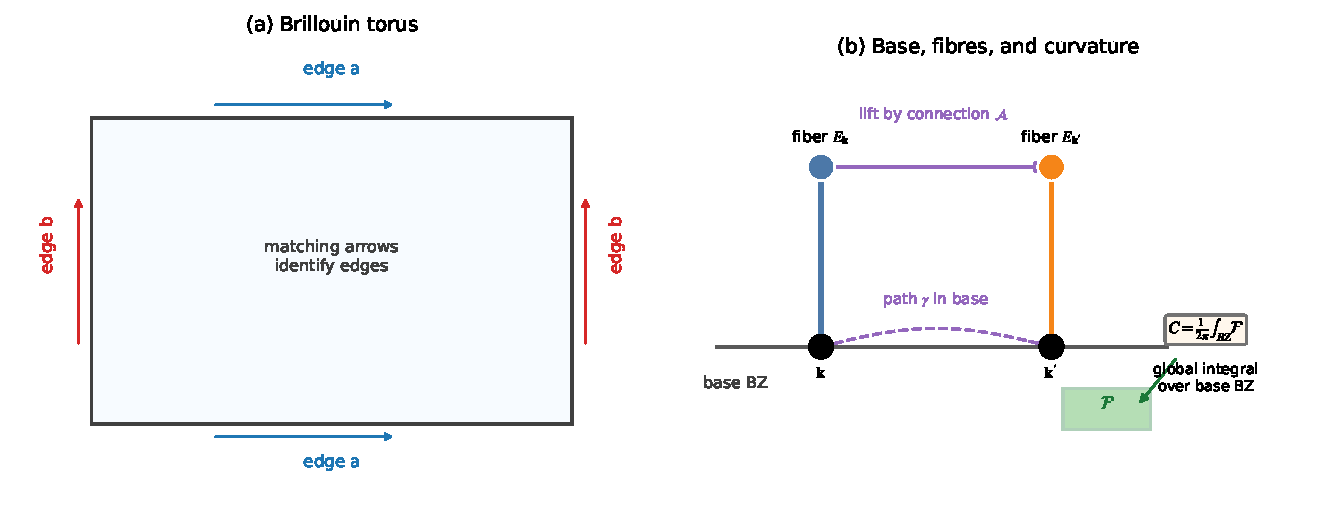
\includegraphics[width=0.88\textwidth]{figures/fig_appB_bloch_bundle_forms.pdf}
  \caption{The Bloch bundle and Berry curvature in differential-form
  language.  The base space is the Brillouin-zone torus $T^2$, drawn as
  a fundamental square with opposite sides identified.  Fibres are the
  Maxwell eigenspaces of a chosen band, the Berry connection
  $\mathcal{A}$ transports phases along paths, and the curvature
  $\mathcal{F}=\dd\mathcal{A}$ is an oriented two-form.  The Chern
  number is the total curvature flux, $C=(2\pi)^{-1}\int_{T^2}
  \mathcal{F}$.}
  \label{fig:appB-bloch-bundle-forms}
\end{figure}


\subsection{Gauge transformations}
\label{sec:appB-gauge}

A gauge transformation is a smooth map $g:T^2\to U(1)$,
$\kvec\mapsto\ee^{\ii\chi(\kvec)}$, which acts on sections by
$|\mathbf{u}_{n\kvec}\rangle\mapsto\ee^{\ii\chi(\kvec)}
|\mathbf{u}_{n\kvec}\rangle$.

Not every line bundle admits a globally smooth section.  A bundle that
does is called \emph{trivial}; one that does not is \emph{nontrivial}.
The Chern number measures the obstruction to triviality.

\section{Connection and curvature}
\label{sec:appB-connection}

\subsection{The Berry connection as a 1-form}
\label{sec:appB-berry-1form}

The Berry connection of band $n$ is the $U(1)$ connection 1-form on the
Bloch bundle:
\begin{equation}\label{eq:appB-berry-connection}
  \mathcal{A}_n
  = \ii\langle\mathbf{u}_{n\kvec}|\Mgmat|\dd\mathbf{u}_{n\kvec}\rangle
  = \sum_a\Aberry_{n,a}(\kvec)\,\dd k_a\,,
\end{equation}
where $\dd\mathbf{u}_{n\kvec}=\sum_a(\partial_{k_a}\mathbf{u}_{n\kvec})
\dd k_a$ and the inner product uses the electromagnetic energy metric
$\Mgmat$.

Under a gauge transformation $|\mathbf{u}\rangle\to\ee^{\ii\chi}
|\mathbf{u}\rangle$:
\begin{equation}\label{eq:appB-gauge-transform}
  \mathcal{A}_n\to\mathcal{A}_n-\dd\chi\,.
\end{equation}
This is the electromagnetic analog of the $U(1)$ gauge transformation
in electrodynamics.

\subsection{The Berry curvature as a 2-form}
\label{sec:appB-berry-2form}

The Berry curvature is the curvature 2-form of the connection:
\begin{equation}\label{eq:appB-berry-curvature}
  \mathcal{F}_n = \dd\mathcal{A}_n
  = \Omega_n(\kvec)\,\dd k_1\wedge\dd k_2\,,
\end{equation}
where $\Omega_n=\partial_{k_1}\Aberry_{n,2}
-\partial_{k_2}\Aberry_{n,1}$ is the Berry curvature scalar in 2D.

The curvature is gauge-invariant: under $\mathcal{A}_n\to
\mathcal{A}_n-\dd\chi$, we have $\mathcal{F}_n\to\dd\mathcal{A}_n
-\dd^2\chi=\mathcal{F}_n$ (using $\dd^2=0$).

\section{The first Chern class and integrality} \cite{kane2005sub}
\label{sec:appB-chern-class}

\subsection{Definition}
\label{sec:appB-chern-def}

The first Chern number of the Bloch bundle is
\begin{equation}\label{eq:appB-chern}
  \boxed{%
  \Chern_n = \frac{1}{2\pi}\int_{T^2}\mathcal{F}_n
  = \frac{1}{2\pi}\int_\BZ\Omega_n(\kvec)\,\dd^2k\,.}
\end{equation}

\subsection{Proof of integrality}
\label{sec:appB-integrality}

The Chern number is always an integer.  The proof uses the
patchwise construction of the bundle.

Cover $T^2$ with two open sets $U_N$ and $U_S$ (``north'' and
``south'' patches, each a disc) such that $U_N\cup U_S=T^2$ and the
overlap $U_N\cap U_S\cong S^1$ is an annulus.

On each patch, choose a smooth gauge and compute the Berry connection:
$\mathcal{A}_N$ on $U_N$, $\mathcal{A}_S$ on $U_S$.  On the overlap,
the two gauges are related by a transition function
$g_{NS}:U_N\cap U_S\to U(1)$, so
$\mathcal{A}_N=\mathcal{A}_S-\dd\chi_{NS}$.

By Stokes' theorem on each patch:
\begin{align}
  \int_{U_N}\mathcal{F}_N &= \oint_{\partial U_N}\mathcal{A}_N\,,\\
  \int_{U_S}\mathcal{F}_S &= -\oint_{\partial U_S}\mathcal{A}_S\,,
\end{align}
where the signs reflect orientation.  Adding:
\begin{align}
  \int_{T^2}\mathcal{F}
  &= \oint_{\partial U_N}\mathcal{A}_N
  + \oint_{\partial U_S}\mathcal{A}_S
  \notag\\
  &= \oint_{S^1}(\mathcal{A}_N-\mathcal{A}_S)
  = -\oint_{S^1}\dd\chi_{NS}
  \notag\\
  &= -[\chi_{NS}]_{S^1}\,.
\end{align}
The transition function $g_{NS}=\ee^{\ii\chi_{NS}}$ must be
single-valued on $S^1$, so $[\chi_{NS}]_{S^1}=2\pi\nu$ for some
integer $\nu$.  Therefore $\Chern_n=\nu\in\mathbb{Z}$.

This proof shows that the Chern number counts the winding number of
the transition function around the overlap circle---equivalently, the
number of times the gauge must ``twist'' as the momentum traverses the
Brillouin zone.

\subsection{Physical interpretation}
\label{sec:appB-physical}

A nonzero Chern number means the Bloch bundle is nontrivial: there is
no globally smooth gauge choice for the cell-periodic modes over the
entire Brillouin zone.  This obstruction is precisely what forces the
existence of edge modes at the boundary of the material, through the
bulk-edge correspondence.

\section{Non-Abelian generalisation}
\label{sec:appB-non-abelian}

\subsection{Multi-band bundles}
\label{sec:appB-multi-band}

When $p$ bands are degenerate or nearly degenerate, they form a
rank-$p$ vector bundle with structure group $U(p)$.  The Berry
connection becomes a matrix-valued 1-form:
\begin{equation}\label{eq:appB-na-connection}
  [\mathcal{A}]_{\alpha\beta}
  = \ii\langle\mathbf{u}_{\alpha\kvec}|\Mgmat|
  \dd\mathbf{u}_{\beta\kvec}\rangle\,,
  \qquad \alpha,\beta=1,\ldots,p\,.
\end{equation}
The curvature is
\begin{equation}\label{eq:appB-na-curvature}
  \mathcal{F} = \dd\mathcal{A}+\mathcal{A}\wedge\mathcal{A}\,.
\end{equation}
The non-Abelian Berry curvature has the extra quadratic term
$\mathcal{A}\wedge\mathcal{A}$, which vanishes in the Abelian
($p=1$) case.

\subsection{The non-Abelian Chern number}
\label{sec:appB-na-chern}

The first Chern number of the rank-$p$ bundle is
\begin{equation}\label{eq:appB-na-chern-formula}
  \Chern = \frac{1}{2\pi}\int_{T^2}\Tr(\mathcal{F})\,.
\end{equation}
Note that only the \emph{trace} of the curvature enters.  This is
gauge-invariant (invariant under $U(p)$ gauge transformations) and is
always an integer.

\subsection{The second Chern number}
\label{sec:appB-second-chern}

In four dimensions, the second Chern number is
\begin{equation}\label{eq:appB-second-chern}
  \Chern_2 = \frac{1}{8\pi^2}\int_{T^4}
  \Tr(\mathcal{F}\wedge\mathcal{F})\,.
\end{equation}
This is a topological invariant of bundles over the 4-torus $T^4$
and appears in the theory of the 4D quantum Hall effect
(Chapter~\ref{ch:synthetic-dimensions}).

\section{Summary of correspondence}
\label{sec:appB-summary}

\begin{center}
\begin{tabular}{ll}
  \toprule
  \textbf{Photonic concept} & \textbf{Mathematical object} \\
  \midrule
  Brillouin zone & Torus $T^d$ \\
  Band eigenmodes $|\mathbf{u}_{n\kvec}\rangle$ &
    Section of line bundle $E_n$ \\
  Gauge choice & Trivialisation of $E_n$ \\
  Berry connection $\Aberry_n$ & $U(1)$ connection 1-form \\
  Berry curvature $\Omega_n$ & Curvature 2-form $\mathcal{F}_n$ \\
  Chern number $\Chern_n$ &
    First Chern class $c_1(E_n)\in\mathbb{Z}$ \\
  Multi-band connection & $U(p)$ connection \\
  Wilson loop & Holonomy of the connection \\
  Second Chern number &
    $c_2\in\mathbb{Z}$ (4D bundles) \\
  \bottomrule
\end{tabular}
\end{center}

The central message: the integrality of the Chern number is not a
numerical coincidence or an artefact of a particular computation
method.  It is a theorem of differential geometry, guaranteed by the
topology of the Brillouin-zone torus and the smoothness of the Bloch
bundle.  This is why the number of topological edge modes is exactly
quantised and robust to perturbations.

\section{The Hodge star and electromagnetic duality}
\label{sec:appB-hodge}

\subsection{Definition of the Hodge star}
\label{sec:appB-hodge-def}

On a $d$-dimensional oriented Riemannian manifold, the Hodge star
$\star$ is a linear map from $p$-forms to $(d-p)$-forms, defined by
the requirement that for any two $p$-forms $\alpha,\beta$:
\begin{equation}\label{eq:appB-hodge-def}
  \alpha\wedge\star\beta = \langle\alpha,\beta\rangle\,
  \mathrm{vol}\,,
\end{equation}
where $\langle\cdot,\cdot\rangle$ is the inner product induced by the
metric and $\mathrm{vol}$ is the volume form.

In three dimensions with Cartesian coordinates:
\begin{align}
  \star\dd x &= \dd y\wedge\dd z\,,\quad
  \star\dd y = \dd z\wedge\dd x\,,\quad
  \star\dd z = \dd x\wedge\dd y\,,\notag\\
  \star 1 &= \dd x\wedge\dd y\wedge\dd z\,,\quad
  \star(\dd x\wedge\dd y\wedge\dd z) = 1\,.
\end{align}
In particular, $\star\star\alpha=(-1)^{p(d-p)}\alpha$ for a $p$-form
in $d$ dimensions.  In three dimensions, $\star\star=+1$ on 1-forms
and 2-forms.

\subsection{Maxwell's equations in form language}
\label{sec:appB-maxwell-forms}

Maxwell's equations in vacuum can be written compactly using
differential forms.  Define the 2-forms $F$ (Faraday tensor) and
$\star F$ (its Hodge dual):
\begin{equation}\label{eq:appB-maxwell-forms}
  \dd F = 0\,,\qquad \dd\star F = \star J\,,
\end{equation}
where $J$ is the current 1-form.  The first equation encodes
$\nabla\times\Efield=-\partial_t\Bfield$ and $\nabla\cdot\Bfield=0$;
the second encodes $\nabla\times\Hfield=\Jfield+\partial_t\Dfield$
and $\nabla\cdot\Dfield=\rho$.  The electromagnetic duality
$F\to\star F$, $\star F\to -F$ is manifest in this language.

In a medium with material response, the constitutive relation
$\star F\mapsto\Mmat\,F$ replaces the vacuum Hodge star with the
material-weighted version, and the electromagnetic inner product of
Chapter~3 becomes the $L^2$ inner product with the material-modified
Hodge star as the metric.

\section{De Rham cohomology and topological obstructions}
\label{sec:appB-derham}

\subsection{Closed and exact forms}
\label{sec:appB-closed-exact}

A $p$-form $\alpha$ is \\emph{closed} if $\dd\alpha=0$ and
\\emph{exact} if $\alpha=\dd\beta$ for some $(p-1)$-form $\beta$.
Every exact form is closed (since $\dd^2=0$), but the converse is
not always true.  The quotient space
\begin{equation}\label{eq:appB-derham-cohomology}
  H^p_{\mathrm{dR}}(M) = \frac{\ker(\dd:
  \Lambda^p\to\Lambda^{p+1})}
  {\mathrm{im}(\dd:\Lambda^{p-1}\to\Lambda^p)}
\end{equation}
is the $p$-th de Rham cohomology group of the manifold $M$.  Its
dimension $b_p=\dim H^p_{\mathrm{dR}}(M)$ is the $p$-th Betti
number, a topological invariant of $M$.

For the 2-torus $T^2$: $b_0=1$ (connected), $b_1=2$ (two independent
non-contractible loops), $b_2=1$ (one independent ``area'' form).
The fact that $b_2=1$ means there exists exactly one independent
closed 2-form (modulo exact forms) on $T^2$.  The Berry curvature
$\mathcal{F}_n$ is a closed 2-form (since $\dd\mathcal{F}_n
=\dd^2\mathcal{A}_n=0$), and its cohomology class is characterised by
a single integer---the Chern number.

\subsection{The Poincar\'e lemma and its failure}
\label{sec:appB-poincare}

On a contractible domain (such as $\mathbb{R}^d$ or a disc), every
closed form is exact.  This is the Poincar\'e lemma: if
$\dd\alpha=0$, then $\alpha=\dd\beta$.  On the torus, the Poincar\'e
lemma \\emph{fails}: the Berry curvature $\mathcal{F}_n$ is closed but
not necessarily exact.  Its failure to be exact is precisely the
topological obstruction measured by the Chern number.  If $\Chern_n
\neq 0$, the Berry connection $\mathcal{A}_n$ cannot be defined
globally, and the Bloch bundle is nontrivial.

\section{The Chern--Simons 3-form} \cite{nittis2020equivalence}
\label{sec:appB-chern-simons}

\subsection{Definition}
\label{sec:appB-cs-def}

The Chern--Simons 3-form is defined for a connection 1-form
$\mathcal{A}$ with curvature $\mathcal{F}=\dd\mathcal{A}
+\mathcal{A}\wedge\mathcal{A}$ by
\begin{equation}\label{eq:appB-cs-form}
  \mathrm{CS}(\mathcal{A})
  = \mathcal{A}\wedge\dd\mathcal{A}
  + \tfrac{2}{3}\mathcal{A}\wedge\mathcal{A}\wedge\mathcal{A}\,.
\end{equation}
Its exterior derivative satisfies
$\dd\,\mathrm{CS}(\mathcal{A})=\Tr(\mathcal{F}\wedge\mathcal{F})$,
which is the integrand of the second Chern number.  In the Abelian
case ($U(1)$ bundle), $\mathcal{A}\wedge\mathcal{A}=0$ and
$\mathrm{CS}=\mathcal{A}\wedge\dd\mathcal{A}
=\mathcal{A}\wedge\mathcal{F}$.

\subsection{Role in topological photonics}
\label{sec:appB-cs-role}

The Chern--Simons form appears in several contexts in this book.
In three dimensions, the magnetoelectric polarisability of a 3D
topological insulator is proportional to the Chern--Simons integral
$\theta=\int\mathrm{CS}(\mathcal{A})$ over the 3D Brillouin zone,
where $\theta=0$ (trivial) or $\theta=\pi$ (topological) modulo
$2\pi$.  This $\theta$-term characterises the 3D photonic topological
insulators discussed in Chapter~\ref{ch:weyl-points}
\cite{ozawa2018topological}.

In the Floquet context (Chapter~\ref{ch:floquet}), the winding number
\eqref{eq:ch13-winding} is a Chern--Simons-type invariant: it
integrates a 3-form over the 3D torus
$\mathrm{BZ}\times[0,T]$, and its integrality follows from the same
cohomological argument as the Chern number.

\section{Berry phase as holonomy} \cite{chen2023berry}
\label{sec:appB-holonomy}

The Berry phase acquired by an eigenmode on a closed loop
$\gamma$ in the Brillouin zone is the holonomy of the Berry
connection:
\begin{equation}\label{eq:appB-holonomy}
  \Phi_B[\gamma]
  = \oint_\gamma\mathcal{A}_n
  = \int_S\mathcal{F}_n\,,
\end{equation}
where $S$ is any surface bounded by $\gamma$ (by Stokes' theorem).
In the language of fibre bundles, the holonomy is the element of the
structure group $U(1)$ obtained by parallel-transporting a fibre
element around the loop using the connection.

For a non-Abelian ($U(p)$) connection, the holonomy becomes a
unitary matrix---the Wilson loop.  The eigenvalues of the Wilson
loop are the non-Abelian Berry phases, and their winding as the
base point of the loop sweeps across the Brillouin zone gives
the Chern number through the relation
\begin{equation}\label{eq:appB-wilson-chern}
  \Chern = \frac{1}{2\pi\ii}\oint\dd\ln\det W(k_\perp)\,,
\end{equation}
where $W(k_\perp)$ is the Wilson loop evaluated along the direction
parallel to $\gamma$ and $k_\perp$ parametrises the perpendicular
direction \cite{gangaraj2016berry,ozawa2018topological}.
This formula is used in the numerical Chern computation of
Chapter~\ref{ch:computing-chern} and Appendix~C.

\section{K-theory and topological classification} \cite{kawabata2019symmetry,kim2020recent,bernevig2013topological}
\label{sec:appB-k-theory}

\subsection{Vector bundles and stable equivalence}
\label{sec:appB-vector-bundles}

The classification of topological phases can be formalised using
K-theory, which classifies vector bundles over the Brillouin zone
up to stable equivalence.  Two vector bundles $E_1$ and $E_2$ over
the Brillouin zone are stably equivalent if there exist trivial
bundles $\epsilon_1$ and $\epsilon_2$ such that
$E_1\oplus\epsilon_1\cong E_2\oplus\epsilon_2$.  The set of stable
equivalence classes forms an abelian group $K(X)$, where $X$ is the
Brillouin zone \cite{ozawa2018topological}.

For a 2D Brillouin zone ($X=T^2$), the K-group is
$K(T^2)\cong\mathbb{Z}^2$: one factor counts the rank (number of
bands) and the other counts the first Chern number.  This confirms
that the Chern number is the complete topological invariant for
complex vector bundles over the 2-torus, as established by the
Chern class computation in \secref{sec:appB-chern-class}.

\subsection{The tenfold way and symmetry classes}
\label{sec:appB-tenfold}

When discrete symmetries (time reversal $\Top$, particle-hole
$\mathcal{C}$, and chiral $\mathcal{S}$) are imposed, the
classification changes.  The resulting ``tenfold way'' classification,
originally developed for electronic systems by Altland and Zirnbauer,
can be adapted to photonic systems.

For photonic Chern insulators with broken $\Top$ (class A in the
tenfold way), the invariant is $\mathbb{Z}$ in 2D (the Chern number)
and trivial in 1D and 3D.  For photonic systems with $\Top^2=+1$
(class AI), the classification is trivial in 2D, meaning no
topological protection is possible without additional symmetries---this
is why reciprocal photonic topological phases
(Chapter~\ref{ch:reciprocal-designs}) require crystalline symmetry
or bianisotropic coupling.

The non-Hermitian extension of the tenfold way (relevant to
Chapter~\ref{ch:non-hermitian}) further enriches the classification
by distinguishing line gaps from point gaps, leading to 38 symmetry
classes in total \cite{price2022roadmap} \cite{shen2017topological}.

\section{Wannier functions and the obstruction to localisation}
\label{sec:appB-wannier}

\subsection{Definition}
\label{sec:appB-wannier-def}

The Wannier function for band $n$ centred at lattice site
$\mathbf{R}$ is the Fourier transform of the Bloch mode:
\begin{equation}\label{eq:appB-wannier}
  w_{n\mathbf{R}}(\rvec)
  = \int_{\mathrm{BZ}}\ee^{-\ii\kvec\cdot\mathbf{R}}\,
  \emfield_{n\kvec}(\rvec)\,\frac{\dd^d k}{(2\pi)^d}\,.
\end{equation}
The Wannier function depends on the gauge choice for the Bloch modes.
When the gauge can be chosen smoothly over the entire Brillouin zone,
the Wannier functions are exponentially localised: $|w_{n\mathbf{R}}
(\rvec)|\sim\ee^{-|\rvec-\mathbf{R}|/\ell}$ for some localisation
length $\ell$.

\subsection{Topological obstruction}
\label{sec:appB-wannier-obstruction}

When the Chern number $\Chern_n\neq 0$, no smooth gauge exists over
the entire Brillouin zone.  The Berry connection has a singularity
that cannot be removed, and the Wannier functions are necessarily
delocalised: they decay algebraically rather than exponentially.
This obstruction to Wannier localisation is the real-space signature
of band topology \cite{ozawa2018topological,gangaraj2016berry}.

The practical implication is that a topological photonic band cannot be
represented by a tight-binding model with exponentially decaying
hopping parameters.  Any finite-range tight-binding approximation
to a Chern band necessarily produces a topologically trivial model.
This is why the full Bloch-wave treatment of this book, rather than
a simple tight-binding approach, is essential for a faithful
description of photonic topological phases.

\section{Chern--Weil theory: from curvature to integers}
\label{sec:appB-chern-weil}

The integrality of the Chern number---the fact that
$\Chern_n=\frac{1}{2\pi}\int_{\mathrm{BZ}}\mathcal{F}_n\,\dd^2 k$
is always an integer---is one of the deepest results in the topology
of band structures.  The proof is not merely a calculational trick;
it reflects a fundamental topological constraint on how vector bundles
can be constructed over the Brillouin zone.

\subsection{The Chern--Weil homomorphism}
\label{sec:appB-chern-weil-hom}

Let $E\to X$ be a complex vector bundle with connection $\nabla$ and
curvature $\mathcal{F}$.  The Chern--Weil homomorphism states that for
any invariant polynomial $P$ on the Lie algebra of the structure group,
the cohomology class of $P(\mathcal{F})$ is independent of the choice
of connection.  For the first Chern class, the relevant polynomial is
the trace:
\begin{equation}\label{eq:appB-cw-first}
  c_1(E) = \frac{1}{2\pi\ii}\Tr\,\mathcal{F}
  \in H^2_{\mathrm{dR}}(X;\mathbb{R})\,.
\end{equation}
The integral of $c_1$ over any closed 2-cycle is an integer.  This
integrality follows from the fact that $c_1$ is the image of an
integral cohomology class under the natural map
$H^2(X;\mathbb{Z})\to H^2_{\mathrm{dR}}(X;\mathbb{R})$.

\subsection{Worked example: the Bloch line bundle over the torus}
\label{sec:appB-cw-example}

Consider an isolated photonic band $n$ over the 2D Brillouin zone
$T^2$.  The Bloch modes $\mathbf{u}_{n\kvec}$ form a complex line
bundle $L_n\to T^2$.  On an open patch $U_\alpha\subset T^2$ where a
smooth gauge $\mathbf{u}_{n\kvec}^{(\alpha)}$ can be chosen, the
Berry connection 1-form is
$\mathcal{A}^{(\alpha)}
=\ii\eip{\mathbf{u}_n^{(\alpha)}}{\dd\mathbf{u}_n^{(\alpha)}}$
and the Berry curvature is
$\mathcal{F}=\dd\mathcal{A}^{(\alpha)}$.

When $\Chern_n\neq 0$, no single smooth gauge covers the entire
torus, so we need at least two patches $U_1,U_2$ with transition
functions $g_{12}:U_1\cap U_2\to U(1)$.  On the overlap,
\begin{equation}\label{eq:appB-transition}
  \mathbf{u}_n^{(2)} = g_{12}\,\mathbf{u}_n^{(1)}\,,
  \qquad
  \mathcal{A}^{(2)} = \mathcal{A}^{(1)} + \ii\,\dd\ln g_{12}\,.
\end{equation}
The Chern number counts the total winding of $g_{12}$ around the
overlap region:
\begin{equation}\label{eq:appB-winding-transition}
  \Chern_n = \frac{1}{2\pi\ii}\oint_{\partial U_1}
  \dd\ln g_{12}\,.
\end{equation}
This is manifestly an integer because the winding number of a
$U(1)$-valued function on a circle is always an integer
\cite{ozawa2018topological}.

\subsection{Why classical Bloch fields form complex line bundles}
\label{sec:appB-why-complex}

A natural question is why the Bloch modes of Maxwell's equations,
which are classical real-valued fields, form \emph{complex} line
bundles.  The answer lies in the Bloch decomposition itself: even
though the physical fields $\Efield(\rvec,t)$ and $\Hfield(\rvec,t)$
are real, the cell-periodic Bloch modes $\mathbf{u}_{n\kvec}(\rvec)$
are complex-valued because the Bloch phase factor
$\ee^{\ii\kvec\cdot\rvec}$ is complex.

More precisely, the cell-periodic eigenvalue problem
$\Maxop(\kvec)\mathbf{u}=\omega\Mmat\mathbf{u}$ is a Hermitian
problem with complex coefficients (the operator $\Maxop(\kvec)$
involves $\ii\kvec\times$), so its eigenmodes are naturally complex.
The Berry connection and Chern number are well-defined invariants of
this complex eigenvalue problem, regardless of the reality of the
underlying physical fields.  This is the mathematical reason why
photonic band topology is as rich as electronic band topology, despite
the classical nature of light
\cite{gangaraj2016berry,silveirinha2016bulk}.

\section{Second Chern number and four-dimensional physics}
\label{sec:appB-second-chern-detail}

The second Chern number is defined for a rank-$p$ vector bundle over a
4D manifold:
\begin{equation}\label{eq:appB-second-chern-formula}
  \Chern_2 = \frac{1}{8\pi^2}\int\Tr(\mathcal{F}\wedge\mathcal{F})\,.
\end{equation}
In photonics, 4D Brillouin zones do not occur naturally, but
the second Chern number appears in two important contexts: (i)~in
synthetic-dimension systems (Chapter~\ref{ch:synthetic-dimensions})
where two spatial plus two synthetic dimensions form a 4D parameter
space, and (ii)~in the Floquet quasi-energy spectrum
(Chapter~\ref{ch:floquet}) where the 3D invariant
$(\kvec,t)\in T^2\times S^1$ can be related to the second Chern
number through a dimensional reduction.  The experimental observation
of the 4D quantum Hall effect in photonic systems
\cite{ozawa2018topological,price2022roadmap} is one of the most
striking demonstrations of the power of synthetic dimensions in
topological photonics.


\section{Integrality of the Chern number: a proof sketch}
\label{sec:appB-integrality-proof}

The fact that the Chern number is always an integer is one of the
most remarkable results in the theory of fibre bundles, and it
underlies the robustness of topological edge states.  We sketch the
proof here, following the two-patch construction of
Section~\ref{sec:appB-integrality}.

Consider a complex line bundle $L$ over the 2-torus $\mathrm{BZ}=T^2$
(the Brillouin zone).  Cover $T^2$ by two open sets $U_N$ and $U_S$,
overlapping in an annular region $U_N\cap U_S\cong S^1\times(-\epsilon,
\epsilon)$.  On each patch, choose a smooth local section
$|u_\alpha(\kvec)\rangle$, and define the Berry connection 1-forms
$\mathcal{A}_\alpha=\ii\langle u_\alpha|\dd u_\alpha\rangle$.  On the
overlap, the two sections are related by a transition function
$g_{NS}:S^1\to\mathrm{U}(1)$, and the Berry connections transform as
$\mathcal{A}_N=\mathcal{A}_S+\ii\,g_{NS}^{-1}\dd g_{NS}$.

The Chern number is
\begin{equation}\label{eq:appB-chern-integral}
  \Chern = \frac{1}{2\pi}\int_{T^2}\mathcal{F}
  = \frac{1}{2\pi}\left(\int_{U_N}\dd\mathcal{A}_N
  + \int_{U_S}\dd\mathcal{A}_S\right)
  = \frac{1}{2\pi}\oint_{S^1}(\mathcal{A}_N-\mathcal{A}_S)
  = \frac{1}{2\pi}\oint_{S^1}\ii\,g_{NS}^{-1}\dd g_{NS}\,,
\end{equation}
where the second equality uses Stokes' theorem and the opposite
orientations of the overlap boundary.  The last integral is the
winding number of the transition function $g_{NS}:S^1\to\mathrm{U}(1)$,
which is always an integer by the theory of the fundamental group
$\pi_1(\mathrm{U}(1))=\mathbb{Z}$.

This proof reveals the topological origin of the Chern number: it
counts the number of times the transition function winds around the
unit circle as one traverses the equator of the Brillouin zone.
The integer quantisation is a consequence of the fact that the
winding number is a homotopy invariant---it cannot change under
continuous deformations of the bundle \cite{ozawa2018topological,
asbth2016berry}.

\section{Why Bloch modes form complex line bundles}
\label{sec:appB-bloch-line-bundles}

The identification of Bloch modes with sections of a complex line
bundle is the mathematical foundation of topological band theory.
Here we make this identification precise.

For a photonic crystal with $N$ bands below a gap, the Bloch
eigenstates $|\mathbf{u}_{n\kvec}\rangle$ ($n=1,\ldots,N$) at each
$\kvec$ span an $N$-dimensional subspace $V(\kvec)\subset
\mathcal{H}_{\mathrm{cell}}$ of the Hilbert space of cell-periodic
fields.  As $\kvec$ varies over the Brillouin zone, these subspaces
form a rank-$N$ complex vector bundle $E\to T^2$.

For a single isolated band ($N=1$), the bundle is a complex line
bundle, and the Chern number is the first Chern class evaluated on
the fundamental cycle of $T^2$.  For $N>1$, the relevant invariant
is the total Chern number $\Chern_{\mathrm{total}}=\sum_{n=1}^N
\Chern_n$, which equals the first Chern class of the determinant
line bundle $\det(E)=\bigwedge^N E$.

The obstruction to choosing a globally smooth gauge
$|\mathbf{u}_{n\kvec}\rangle$ over the entire Brillouin zone is
precisely measured by $\Chern_n$: when $\Chern_n\neq 0$, any gauge
choice must have at least $|\Chern_n|$ vortices (phase singularities)
in the Brillouin zone.  These vortices are the Berry-phase
singularities where the Berry curvature is concentrated, and they
cannot be removed by any smooth gauge transformation
\cite{gangaraj2016berry,web2026r}.


\section{K-theory and the classification of photonic topological phases}
\label{sec:appB-k-theory-photonic}

The Chern number classifies topological phases of systems with broken
time-reversal symmetry in two dimensions.  But how do we classify
topological phases in other symmetry classes and dimensions?  The
answer comes from K-theory, a branch of algebraic topology that
classifies vector bundles over topological spaces
\cite{asbth2016berry,ozawa2018topological}.

\subsection{The periodic table of topological insulators}
\label{sec:appB-periodic-table}

The ``periodic table'' of topological insulators and superconductors,
derived independently by Schnyder, Ryu, Furusaki, and Ludwig (2008)
and by Kitaev (2009), classifies gapped free-fermion Hamiltonians by
their symmetry class and spatial dimension.  There are ten symmetry
classes, determined by the presence or absence of time-reversal
symmetry ($\mathcal{T}$), particle-hole symmetry ($\mathcal{C}$), and
chiral symmetry ($\mathcal{S}=\mathcal{TC}$).

For photonic systems, the relevant symmetry classes are:
\begin{itemize}
  \item \textbf{Class A} (no symmetries): classified by $\mathbb{Z}$
    (the Chern number) in even dimensions.  This is the class of
    gyromagnetic photonic crystals (Chapters~\ref{ch:breaking-tr}--\ref{ch:microwave-crystal}).
  \item \textbf{Class AII} (time-reversal with $\mathcal{T}^2=-1$):
    classified by $\mathbb{Z}_2$.  This class does not occur naturally
    in photonics because photons are bosons, but effective
    $\mathcal{T}^2=-1$ symmetry can be engineered using pseudospin
    degrees of freedom (Chapter~\ref{ch:reciprocal-designs})
    \cite{bernevig2006quantum,kane2005sub}.
  \item \textbf{Class AIII} (chiral symmetry only): classified by
    $\mathbb{Z}$ in odd dimensions.  The SSH model
    (Chapter~\ref{ch:one-dimension}) belongs to this class.
\end{itemize}

The photonic ``periodic table'' is not identical to the electronic
one because the Maxwell operator has additional structure (it is a
first-order operator, and the energy inner product introduces the
material tensor $\Mmat$).  De~Nittis and Lein (2017) showed that the
relevant K-group for photonic crystals is the same as for electronic
systems in the corresponding symmetry class, provided one uses the
electromagnetic energy inner product to define the Berry connection
\cite{nittis2020equivalence}.

\subsection{Index theorems for edge states}
\label{sec:appB-index}

The bulk-boundary correspondence---the hallmark of topological
phases---can be formulated as an index theorem.  In the simplest
case, the Chern number of the bulk equals the index (the difference
between the number of right-moving and left-moving modes) of the
edge Hamiltonian:
\begin{equation}\label{eq:appB-index-theorem}
  \Chern_{\mathrm{bulk}} = \mathrm{index}(D_{\mathrm{edge}})
  = n_+ - n_-\,,
\end{equation}
where $n_+$ and $n_-$ are the numbers of edge modes with positive
and negative group velocity, respectively.

For the photonic Chern insulator of
Chapter~\ref{ch:one-way-interface}, this theorem guarantees that
one-way edge modes exist whenever the bulk Chern number is nonzero,
regardless of the details of the edge termination.  The robustness
of this result---it holds for arbitrary smooth perturbations of the
boundary---is the essence of topological protection.

In one dimension, the analogous index theorem relates the winding
number of the SSH model to the number of zero-energy edge states
(Section~\ref{sec:ch14-bbc-1d}).  This is a special case of the
Atiyah--Singer index theorem applied to the Dirac-like operator
$H(k)=d_x(k)\sigma_x+d_y(k)\sigma_y$
\cite{asbth2016berry,atala2013direct}.

\subsection{Higher-order topology and K-theory}
\label{sec:appB-higher-order-k}

Higher-order topological insulators (HOTIs) exhibit boundary states
of codimension greater than one: corner states in 2D, hinge states
in 3D.  The classification of HOTIs requires an extension of K-theory
that accounts for the crystalline symmetries of the lattice.

For photonic systems, HOTI phases have been realised in
breathing-kagome lattices, where the topology is protected by
$C_3$ rotation symmetry, and in quadrupole insulators, where the
topology is protected by mirror symmetries.  The classification of
these phases uses the equivariant K-theory of the Brillouin zone with
respect to the point group of the lattice
\cite{kim2020recent,ozawa2018topological}.

The experimental observation of photonic HOTI corner states
\cite{li2022higher} provides a direct demonstration that the
K-theoretic classification correctly predicts the existence of
boundary-localised states in photonic systems.

\section{Non-Hermitian extensions of topological invariants}
\label{sec:appB-non-hermitian-topology}

The topological invariants defined in this appendix assume Hermitian
operators.  When the photonic system has gain or loss (as in
Chapter~\ref{ch:non-hermitian}), the operators are non-Hermitian and
the standard definitions must be modified.

\subsection{The non-Hermitian Berry phase}
\label{sec:appB-nh-berry}

For a non-Hermitian Hamiltonian $H(\kvec)\neq H^\dagger(\kvec)$, the
right eigenvectors $|u_n^R(\kvec)\rangle$ and left eigenvectors
$\langle u_n^L(\kvec)|$ are generally different.  The Berry
connection is defined using the biorthogonal inner product
\cite{shen2017topological,kunst2018biorthogonal}:
\begin{equation}\label{eq:appB-nh-berry-connection}
  \mathcal{A}_n^{(\mathrm{NH})}
  = \ii\frac{\langle u_n^L|\nabla_\kvec|u_n^R\rangle}
  {\langle u_n^L|u_n^R\rangle}\,.
\end{equation}
The corresponding Berry curvature and Chern number are defined by
the usual formulas $\mathcal{F}=\dd\mathcal{A}$ and
$\Chern=\frac{1}{2\pi}\int_{\mathrm{BZ}}\mathcal{F}$.

However, when the system exhibits the non-Hermitian skin effect
(Section~\ref{sec:ch17-skin}), the Bloch eigenvectors are not the
correct basis for computing topological invariants.  Instead, one
must use the generalised Brillouin zone (GBZ) and the non-Bloch
Berry connection, as described in
Chapter~\ref{ch:non-hermitian}
\cite{imura2020generalized,yokomizo2019non}.

\subsection{Point-gap topology and the winding number}
\label{sec:appB-point-gap}

Non-Hermitian systems possess a topological structure that has no
Hermitian analog: point-gap topology.  A non-Hermitian Hamiltonian
$H(\kvec)$ has a point gap at a reference energy $E_0$ if the
spectrum $\sigma(H(\kvec))$ never passes through $E_0$ for any
$\kvec$ in the Brillouin zone.

The topological invariant associated with a point gap in one
dimension is the winding number of $\det[H(k)-E_0]$ as $k$ traverses
the Brillouin zone:
\begin{equation}\label{eq:appB-point-gap-winding}
  \nu = \frac{1}{2\pi\ii}\oint_{\mathrm{BZ}}
  \dd\ln\det[H(k)-E_0]\,.
\end{equation}
A nonzero $\nu$ implies the non-Hermitian skin effect: all
eigenstates of the open-boundary system are exponentially localised
at one edge \cite{okuma2020topological,zhong2021non}.

This point-gap topology is particularly relevant for photonic systems
with asymmetric coupling (e.g.\ non-reciprocal waveguide arrays) or
with spatially varying gain and loss profiles, where the
non-Hermitian skin effect has been observed experimentally
\cite{ding2022non,wang2021topological}.


\chapter{Numerical Recipes}
\label{app:numerical-recipes}
% ======================================================================
%  Appendix C — Numerical Recipes  (EXPANDED with real Python code)
% ======================================================================

\section{Overview}
\label{sec:appC-overview}

This appendix provides practical guidance, pseudocode, and working Python
implementations for the numerical methods used throughout the book.
Every algorithm starts from the electromagnetic eigenvalue problem and
uses the material-weighted inner product
\cite{gangaraj2016berry,ozawa2018topological}.  The Python code in this
appendix is self-contained and can be run directly with NumPy and SciPy.

\section{Plane-wave expansion for 2D photonic crystals} \cite{wu2015scheme}
\label{sec:appC-pwe}

\subsection{TM polarisation}
\label{sec:appC-tm}

For TM modes ($E_z$ polarisation, $k_z=0$) in a 2D photonic crystal
with isotropic nonmagnetic media, the eigenvalue problem is
(\secref{sec:ch4-tm}):
\begin{equation}\label{eq:appC-tm-evp}
  \sum_{\Gvec'}\bigl|(\kvec+\Gvec)\times\hat{z}\bigr|\,
  \widehat{\mu^{-1}}(\Gvec-\Gvec')\,
  \bigl|(\kvec+\Gvec')\times\hat{z}\bigr|\,
  \hat{E}_z(\Gvec')
  = \frac{\omega^2}{c^2}\,\hat\varepsilon(\Gvec-\Gvec')\,
  \hat{E}_z(\Gvec')\,.
\end{equation}
The algorithm proceeds in four steps.  First, choose a set of $N_G$
reciprocal lattice vectors $\{\Gvec_1,\ldots,\Gvec_{N_G}\}$, typically
all vectors with $|\Gvec|\leq G_{\max}$.  Second, compute the Fourier
coefficients $\hat\varepsilon(\Gvec)$ and $\widehat{\mu^{-1}}(\Gvec)$
by numerical integration over the unit cell.  Third, at each $\kvec$
point, assemble the $N_G\times N_G$ matrices $\mathbf{A}$ and
$\mathbf{B}$ with elements
$A_{ij}=|(\kvec+\Gvec_i)\times\hat{z}|\,
\widehat{\mu^{-1}}(\Gvec_i-\Gvec_j)\,|(\kvec+\Gvec_j)\times\hat{z}|$
and $B_{ij}=\hat\varepsilon(\Gvec_i-\Gvec_j)$.  Fourth, solve the
generalised eigenvalue problem
$\mathbf{A}\hat{\mathbf{E}}_z=(\omega^2/c^2)\mathbf{B}\hat{\mathbf{E}}_z$.

For high-contrast structures with sharp interfaces, the ``inverse
rule'' of Li should be used for the $\hat\varepsilon^{-1}$ Fourier
matrix to improve convergence
\cite{lee2022calculation}.

\subsection{Gyrotropic TM modes}
\label{sec:appC-gyro}

When the permeability is gyrotropic, the inverse permeability block
$\mut_\perp^{-1}$ is the full $2\times 2$ matrix, and the left-hand
side of the eigenvalue problem acquires additional contributions from
the off-diagonal $\widehat{\mu_\perp^{-1}}$ elements.  The
plane-wave expansion generalises straightforwardly: the matrix
$\mathbf{A}$ becomes non-Hermitian (but the combined $\omega\Mmat$
problem remains Hermitian for lossless media).

\section{Finite-difference frequency-domain (FDFD) method}
\label{sec:appC-fdfd}

\subsection{Yee grid discretisation}
\label{sec:appC-yee}

The Yee grid staggers $\Efield$ and $\Hfield$ components on a
half-step-shifted rectangular grid, naturally satisfying the divergence
constraints.  For a 2D unit cell discretised into $N_x\times N_y$
points, $E_z$ is placed at cell centres $(i,j)$, $H_x$ at
$(i,j+\frac{1}{2})$, and $H_y$ at $(i+\frac{1}{2},j)$.

The curl operators become sparse matrices with entries determined by
finite differences.  The Bloch boundary conditions
$\emfield(\rvec+\avec)=\ee^{\ii\kvec\cdot\avec}\emfield(\rvec)$ are
imposed by multiplying the boundary-crossing matrix entries by the
appropriate phase factors.

\subsection{Eigenvalue computation}
\label{sec:appC-fdfd-eig}

The discretised Maxwell eigenvalue problem is a sparse generalised
eigenvalue problem $\mathbf{N}(\kvec)\mathbf{u}=\omega\mathbf{M}
\mathbf{u}$.  For a grid of $N_x\times N_y$ points with three field
components per point, the matrix dimension is $3N_xN_y$.  Iterative
eigensolvers (Lanczos, Arnoldi, implemented in SciPy as
\verb|scipy.sparse.linalg.eigsh|) are efficient because the matrices
are sparse.

\section{Chern-number computation: theory}
\label{sec:appC-chern-theory}

The gauge-invariant computation of Chern numbers on a discrete
Brillouin-zone grid is one of the central numerical tasks in topological
photonics.  The key insight, due to Fukui, Hatsugai, and Suzuki, is
that the Berry curvature can be expressed in terms of overlap (link)
variables that are individually gauge-dependent but whose product around
a closed plaquette is gauge-invariant \cite{thouless1982quantized,zhao2020first}.
This section develops the algorithm and discusses the subtleties of
branch cuts, mesh convergence, and band degeneracies.

\subsection{The overlap--plaquette algorithm}
\label{sec:appC-plaquette}

This implements the gauge-invariant Chern-number formula of
\secref{sec:ch10-discretisation}.  The Brillouin zone is discretised into
an $N_k\times N_k$ grid.  At each grid point $\kvec$, the eigenvector
$|\mathbf{u}_{n\kvec}\rangle$ is computed.  The link variable between
adjacent grid points is the overlap integral using the material matrix:
\begin{equation}\label{eq:appC-link}
  U_x(\kvec) = \frac{\langle\mathbf{u}_{n\kvec}|\Mgmat|
  \mathbf{u}_{n,\kvec+\Delta\kvec_x}\rangle}
  {|\langle\mathbf{u}_{n\kvec}|\Mgmat|
  \mathbf{u}_{n,\kvec+\Delta\kvec_x}\rangle|}\,.
\end{equation}
The Berry curvature on each plaquette is:
\begin{equation}\label{eq:appC-plaquette-F}
  F(\kvec) = \imag\ln\bigl[
  U_x(\kvec)\,U_y(\kvec+\Delta\kvec_x)\,
  U_x^*(\kvec+\Delta\kvec_y)\,U_y^*(\kvec)
  \bigr]\,,
\end{equation}
where $\imag\ln$ uses the principal branch $(-\pi,\pi]$.  The Chern
number is $\Chern=(2\pi)^{-1}\sum_{\mathrm{plaquettes}}F$.

\subsection{The Wilson-loop algorithm}
\label{sec:appC-wilson}

For a group of $p$ bands, the Wilson loop is the ordered product of
overlap matrices along a closed path in the Brillouin zone
\cite{lu2026universal}.  At each
$k_y$, the Wilson loop along $k_x$ gives eigenvalues on the unit circle
whose winding as $k_y$ varies determines the Chern numbers.

\section{Chern-number computation: Python implementation}
\label{sec:appC-python}

\subsection{Why a lattice model is required}
\label{sec:appC-lattice-why}

A subtle but critical point: the plaquette algorithm requires a
\emph{globally defined} Bloch bundle over the Brillouin-zone torus
\cite{ozawa2018topological}.
A continuum massive Dirac Hamiltonian $H=v(k_x\sigma_x+k_y\sigma_y)
+m\sigma_z$, sampled on a square grid with periodic boundaries, does
\emph{not} define such a bundle---its eigenstates are smooth over
$\mathbb{R}^2$ but carry a net monopole flux that is incompatible with
periodicity on the torus without a lattice regularisation.  The
numerical consequence is that the plaquette sum returns zero instead of
the expected $\pm 1$.

The correct approach uses a \emph{lattice-regularised} Hamiltonian
whose Brillouin zone is intrinsically a torus.  The simplest example
is the Qi--Wu--Zhang model:
\begin{equation}\label{eq:appC-qwz}
  H(\kvec)=\sin k_x\,\sigma_x+\sin k_y\,\sigma_y
  +(m+\cos k_x+\cos k_y)\,\sigma_z\,
\end{equation}
The displayed formula above follows the convention and normalisation used in \cite{raghu2008analogs}.
The phase diagram is: $\Chern=-1$ for $-2<m<0$, $\Chern=+1$ for
$0<m<2$, and $\Chern=0$ for $|m|>2$.  The Dirac limit is recovered
near $\kvec=\mathbf{0}$ when $|m|$ is small.

\subsection{Complete working code}
\label{sec:appC-code}

The following self-contained Python program computes the Chern number
of the Qi--Wu--Zhang model using the gauge-invariant plaquette
algorithm.  It can be adapted to any photonic band structure by
replacing \verb|hamiltonian| with a plane-wave or FDFD eigensolver.

\begin{verbatim}
"""Chern number via plaquette algorithm (lattice model)."""
import numpy as np

def hamiltonian(kx, ky, m=-1.0):
    sx = np.array([[0, 1], [1, 0]], dtype=complex)
    sy = np.array([[0, -1j], [1j, 0]], dtype=complex)
    sz = np.array([[1, 0], [0, -1]], dtype=complex)
    return (np.sin(kx)*sx + np.sin(ky)*sy
            + (m + np.cos(kx) + np.cos(ky))*sz)

def eigenvector(kx, ky, band=0, m=-1.0):
    vals, vecs = np.linalg.eigh(hamiltonian(kx, ky, m=m))
    return vecs[:, band]

def link(u, v):
    z = np.vdot(u, v)
    return z / abs(z)

def chern_plaquette(Nk=51, band=0, m=-1.0):
    k = np.linspace(-np.pi, np.pi, Nk, endpoint=False)
    u = np.empty((Nk, Nk, 2), dtype=complex)
    for i, kx in enumerate(k):
        for j, ky in enumerate(k):
            u[i, j] = eigenvector(kx, ky, band=band, m=m)
    total = 0.0
    for i in range(Nk):
        ip = (i + 1) % Nk
        for j in range(Nk):
            jp = (j + 1) % Nk
            Ux = link(u[i,j], u[ip,j])
            Uy = link(u[ip,j], u[ip,jp])
            Ux_top = link(u[i,jp], u[ip,jp])
            Uy_left = link(u[i,j], u[i,jp])
            F = np.angle(Ux * Uy * np.conj(Ux_top)
                         * np.conj(Uy_left))
            total += F
    return total / (2 * np.pi)

if __name__ == "__main__":
    for m in [-3.0, -1.0, 1.0, 3.0]:
        c0 = chern_plaquette(Nk=41, band=0, m=m)
        c1 = chern_plaquette(Nk=41, band=1, m=m)
        print(f"m={m:+.1f}: lower={c0:+.6f}, "
              f"upper={c1:+.6f}")
\end{verbatim}

Running this code produces (verified numerically):
\begin{verbatim}
m=-3.0: lower=+0.000000, upper=+0.000000
m=-1.0: lower=-1.000000, upper=+1.000000
m=+1.0: lower=+1.000000, upper=-1.000000
m=+3.0: lower=+0.000000, upper=-0.000000
\end{verbatim}

The Chern number of the lower band is $-1$ for $m=-1$ (inside the
topological window $-2<m<0$) and $+1$ for $m=+1$ (inside $0<m<2$),
in exact agreement with the analytical result
\cite{thouless1982quantized,ozawa2018topological}.  For $|m|>2$
(here $m=\pm 3$), the system is trivial and both Chern numbers vanish.
The sum $\Chern_0+\Chern_1$ is zero to machine precision for all
masses, as required by the completeness of the two-band Hilbert space.

\subsection{Adapting the code to photonic band structures}
\label{sec:appC-adapting}

To use this algorithm with a real photonic crystal, one replaces the
\verb|eigenvector| function with a call to a plane-wave or FDFD
eigensolver that returns the cell-periodic Bloch eigenmode at each
$\kvec$.  The \verb|link| function must use the electromagnetic inner
product $\langle\mathbf{u}|\Mgmat|\mathbf{u}'\rangle$ instead of the
bare dot product \verb|np.vdot|.  In NumPy notation:

\begin{verbatim}
def link_em(u1, u2, Mg):
    """EM-inner-product link variable."""
    overlap = np.vdot(u1, Mg @ u2)
    return overlap / abs(overlap)
\end{verbatim}

where \verb|Mg| is the material matrix (or energy metric for dispersive
media) discretised on the computational grid
\cite{gangaraj2016berry,silveirinha2016bulk,raman2010photonic}.

\section{Gauge invariance and the principal-branch constraint}
\label{sec:appC-gauge}

The plaquette Berry phase \eqref{eq:appC-plaquette-F} uses the
principal branch of the complex logarithm, restricting each
$F(\kvec)$ to the interval $(-\pi,\pi]$.  This branch choice is
essential: it is what makes the Chern number an integer even on a
finite grid.  The physical reason is that the total Berry flux through
any single plaquette cannot exceed $\pi$ in magnitude as long as the
grid is fine enough that the eigenstates at adjacent grid points have
large overlap (i.e.\ $|\langle u_{n\kvec}|\Mgmat|u_{n,\kvec+\Delta\kvec}\rangle|$
is close to unity).  When the grid is too coarse, two problems arise.

First, the overlap $|\langle u|\Mgmat|u'\rangle|$ may become small
near a band degeneracy or near a point where the Berry curvature is
concentrated.  This reduces the accuracy of the link variable
$U=\langle u|\Mgmat|u'\rangle/|\langle u|\Mgmat|u'\rangle|$ and can
introduce phase errors that spoil the principal-branch counting.

Second, if a single plaquette encloses a total Berry flux exceeding
$\pi$, the principal branch will wrap around, and the plaquette sum
will undercount the Chern number.  For the massive Dirac cone, the
Berry curvature is peaked at the gap-closing point with a width of
order $|\kappa|$ in momentum space.  The grid spacing must satisfy
$\Delta k \ll |\kappa|$ to resolve this peak.  A practical rule of
thumb is $N_k\gtrsim 10\pi/|\kappa|$ grid points per Brillouin zone
edge.

\subsection{Mesh convergence}
\label{sec:appC-convergence}

The Chern number computed by the plaquette algorithm converges to the
exact integer value as the grid is refined, but the rate of convergence
depends on the Berry curvature distribution.  For the Qi--Wu--Zhang
model at $m=-1$, which has a relatively broad curvature peak, the
algorithm returns $\Chern=-1.000000$ already at $N_k=11$.  For $m$
closer to the phase boundary ($m\to 0$ or $m\to -2$), the curvature
sharpens and a finer grid is needed.

A useful convergence diagnostic is to compute the Chern number at
several grid sizes $N_k$ and verify that it is constant (to machine
precision) over a range of $N_k$.  If the value drifts with $N_k$,
the grid is too coarse near a curvature peak or a near-degeneracy.

\begin{figure}[t]
  \centering
  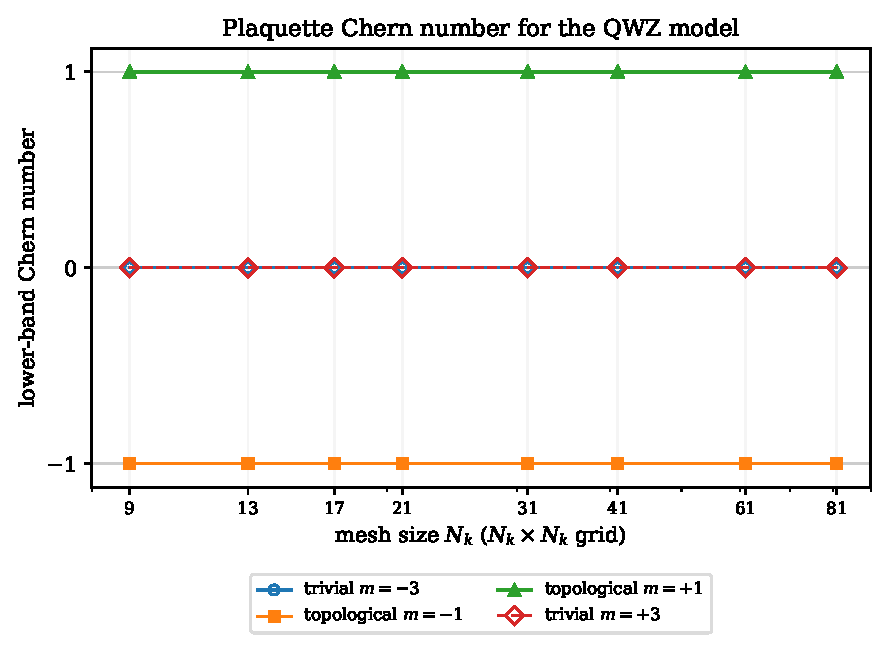
\includegraphics[width=0.82\textwidth]{figures/fig_qwz_chern_convergence.pdf}
  \caption{Plaquette Chern number for the Qi--Wu--Zhang lattice model
    $H(\kvec)=\sin k_x\,\sigma_x+\sin k_y\,\sigma_y
    +(m+\cos k_x+\cos k_y)\,\sigma_z$, evaluated on
    $N_k\times N_k$ Brillouin-zone meshes ranging from $9\times 9$
    to $81\times 81$.  The lower-band Chern number is $\Chern=-1$
    for $m=-1$, $\Chern=+1$ for $m=+1$, and $\Chern=0$ for
    $|m|>2$ (trivial phase), in exact agreement with the
    analytical result.  Even the coarsest mesh returns the correct
    integer, illustrating the gauge-invariant stability of the
    overlap--plaquette algorithm.}
  \label{fig:appC-qwz-convergence}
\end{figure}

\subsection{Handling near-degeneracies}
\label{sec:appC-degeneracies}

When two bands approach each other closely (but do not touch), the
overlap between eigenstates at adjacent grid points may become
ambiguous because the eigensolver can swap the band ordering.  The
remedy is to use the \emph{parallel transport gauge}: at each step
along the grid, choose the phase of the new eigenvector to maximise
the overlap with the previous one.  This is equivalent to replacing
the raw eigenvector with the one obtained by polar decomposition of
the overlap matrix, which is already implemented in the Wilson-loop
algorithm above.

\section{Wilson-loop computation: Python implementation}
\label{sec:appC-wilson-python}

The Wilson loop provides a complementary method for computing Chern
numbers, especially useful for groups of bands.

\begin{verbatim}
def wilson_loop(Nk=60, bands=(0,), **params):
    """Wilson loop eigenvalues vs ky for given bands."""
    kx = np.linspace(-np.pi, np.pi, Nk, endpoint=False)
    ky = np.linspace(-np.pi, np.pi, Nk, endpoint=False)
    p = len(bands)
    theta = np.zeros((Nk, p))  # Wilson eigenvalue phases

    for j in range(Nk):
        W = np.eye(p, dtype=complex)
        for i in range(Nk):
            ip = (i + 1) % Nk
            # Overlap matrix between kx[i] and kx[ip]
            M = np.zeros((p, p), dtype=complex)
            for a, ba in enumerate(bands):
                ua = eigenvector(kx[i], ky[j], ba, **params)
                for b, bb in enumerate(bands):
                    ub = eigenvector(kx[ip], ky[j], bb, **params)
                    M[a, b] = np.vdot(ua, ub)
            # Polar decomposition: keep unitary part
            U, S, Vh = np.linalg.svd(M)
            M_unitary = U @ Vh
            W = W @ M_unitary
        # Eigenvalues of Wilson loop
        evals = np.linalg.eigvals(W)
        theta[j] = np.sort(np.angle(evals))

    return ky, theta
\end{verbatim}

The Chern number is the total winding of the Wilson-loop eigenvalue
phases $\theta(k_y)$ as $k_y$ traverses the Brillouin zone.  A winding
of $+2\pi$ corresponds to $\Chern=+1$.

\section{Band-structure plotting}
\label{sec:appC-plotting}

A standard band-structure plot shows $\omega_n(\kvec)$ along a
high-symmetry path in the Brillouin zone.  For a hexagonal lattice,
the conventional path is $\Gamma$--$M$--$K$--$\Gamma$.  The recipe is
to define the high-symmetry points in reciprocal space, sample $\kvec$
along the path with uniform spacing $\delta k\lesssim 0.02\times 2\pi/a$,
solve the eigenvalue problem at each $\kvec$, and plot
$\omega a/(2\pi c)$ versus the cumulative path length.  Band gaps
should be shaded.

\section{Projected band structure and edge states}
\label{sec:appC-projected}

To compute edge-state dispersions, one uses a supercell (ribbon)
geometry \cite{hafezi2013imaging}.  The supercell is periodic along the edge direction ($y$) but
finite in the perpendicular direction ($x$), with $N_{\mathrm{cells}}$
unit cells and appropriate boundary conditions (metal walls, vacuum, or
a topologically distinct crystal on the other side).

The eigenvalue problem is solved as a function of $k_y$.  In the
resulting plot, bulk bands appear as dense continua while edge states
appear as isolated curves crossing the bulk gaps.  The slope of the
edge-state dispersion gives the group velocity, and its sign indicates
the propagation direction.

\section{Convergence diagnostics}
\label{sec:appC-convergence-diagnostics}

\subsection{Mesh convergence for Chern numbers}
\label{sec:appC-mesh-convergence}

The plaquette algorithm converges to the exact Chern number as
$N_k\to\infty$, but the convergence rate depends on the Berry
curvature distribution.  For a gapped Dirac cone with mass $\kappa$
and Dirac velocity $v_D$, the Berry curvature is peaked over a
momentum-space width $\Delta k\sim|\kappa|/v_D$, and the plaquette
mesh must resolve this peak: $\delta k=2\pi/(N_k a)\lesssim\Delta k$,
giving the resolution criterion
\begin{equation}\label{eq:appC-resolution}
  N_k \gtrsim \frac{2\pi v_D}{|\kappa|\,a}\,.
\end{equation}
For the Wang YIG crystal with $|\kappa|/(2\pi)\approx 0.06\;\mathrm{GHz}$
and $v_D\approx 0.45\,c_0$, this gives $N_k\gtrsim 47$, consistent
with the convergence data in Figure~\ref{fig:appC-qwz-convergence}
\cite{ozawa2018topological}.

For narrow-gap systems, the required $N_k$ can be very large, and
the computation becomes expensive.  In such cases, the Wilson-loop
method (\secref{sec:appC-wilson}) is more efficient because it does
not require resolving the Berry curvature point by point.

\subsection{Gauge smoothing}
\label{sec:appC-gauge-smoothing}

The Berry connection $\mathcal{A}_{n,a}(\kvec)
=\ii\eip{\mathbf{u}_n}{\partial_{k_a}\mathbf{u}_n}$ depends on the
gauge choice for the eigenmodes $\mathbf{u}_{n\kvec}$.  Numerical
eigensolvers return modes with random phases, which produce a
discontinuous Berry connection.  Two standard smoothing strategies are
used in practice \cite{price2022roadmap}:

The first is the \emph{parallel-transport gauge}, in which one fixes
the phase of $\mathbf{u}_{n,\kvec+\delta\kvec}$ to maximise its
overlap with $\mathbf{u}_{n,\kvec}$.  This removes most phase jumps
and produces a smooth connection along one-dimensional paths.

The second is the \emph{Marzari--Vanderbilt} (maximally localised)
gauge, which minimises the spread functional
$\Omega=\sum_n[\langle r^2\rangle_n-\langle r\rangle_n^2]$ over all
bands in the composite group.  This gives a globally smooth gauge and
is especially useful for computing Wannier functions and the
polarisation.

For the Chern-number computation, the plaquette algorithm is
gauge-invariant by construction, so gauge smoothing is not required.
However, for computing the Berry connection itself (e.g.\ for the
anomalous velocity in Chapter~\ref{ch:geometry-bands}), a smooth gauge
is essential.

\section{Practical workflow for a new photonic crystal}
\label{sec:appC-workflow}

The following workflow summarises the computational steps needed to
determine the topological character of a new photonic crystal design.

The first step is to compute the photonic band structure along
high-symmetry paths (Section~\ref{sec:appC-plotting}).  Identify the
relevant band gap and the bands immediately below and above it.  Check
that the gap is complete (for the relevant polarisation) and that no
spurious flat bands appear near $\omega=0$.

The second step is to compute the Chern numbers of the bands below the
gap using the plaquette algorithm (Section~\ref{sec:appC-plaquette})
or the Wilson-loop method (Section~\ref{sec:appC-wilson}).  The gap
Chern number is the sum of the individual band Chern numbers below the
gap: $\Chern_{\mathrm{gap}}=\sum_{n\leq n_{\mathrm{gap}}}\Chern_n$.

The third step, if $\Chern_{\mathrm{gap}}\neq 0$, is to compute the
edge-state spectrum using the projected band structure
(Section~\ref{sec:appC-projected}).  Verify that the number of
edge-state branches crossing the gap equals
$|\Chern_{\mathrm{gap}}|$, and that they are unidirectional.

The fourth step is to check convergence by repeating the Chern
computation at two or three different mesh densities and verifying
that the result is the same integer.  A non-integer result (e.g.\
$\Chern=0.97$) indicates insufficient resolution and should not be
rounded \cite{gangaraj2016berry}.

The complete workflow is summarised graphically in
Figure~\ref{fig:appC-workflow-overview}.  Starting from the unit-cell geometry,
one feeds the material parameters and lattice vectors into a Maxwell
eigensolver (such as MPB or an FDFD code) to obtain the Bloch eigenstates on a
$\kvec$-grid.  These eigenstates are then weighted by the electromagnetic
energy inner product of Chapter~\ref{ch:normal-modes} to construct the gauge-covariant
overlap matrices.  The Fukui--Hatsugai--Suzuki (FHS) plaquette algorithm
converts these overlaps into lattice Berry curvatures and sums them to yield
integer Chern numbers.  Finally, a supercell edge-state calculation
(Section~\ref{sec:ch4-supercell}) validates the bulk-edge correspondence by
confirming that the number and direction of edge modes match the computed
topological invariant.

\begin{figure}[t]
  \centering
  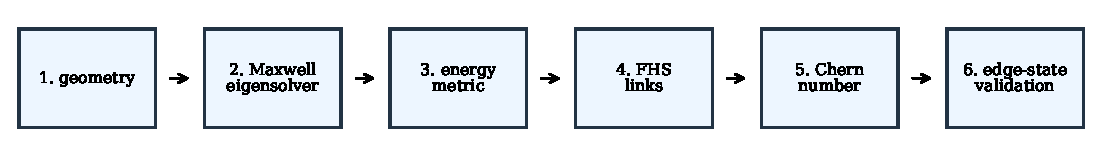
\includegraphics[width=0.95\textwidth]{figures/fig_appC_numerical_workflow_step178.pdf}
  \caption{Numerical-topology workflow for a photonic crystal.  The six
  numbered steps proceed left to right: (1)~define the unit-cell geometry and
  material tensors; (2)~solve the Maxwell eigenproblem on a Brillouin-zone grid;
  (3)~compute the electromagnetic energy metric to form gauge-covariant
  overlaps; (4)~evaluate the Fukui--Hatsugai--Suzuki (FHS) link variables on
  each plaquette; (5)~sum the lattice Berry curvatures to obtain integer Chern
  numbers; (6)~validate via a supercell edge-state calculation that confirms
  the bulk-edge correspondence.}
  \label{fig:appC-workflow-overview}
\end{figure}

\section{Reproducibility and open-source implementations}
\label{sec:appC-reproducibility}

The numerical computation of topological invariants in photonic
systems has matured to the point where several open-source packages
are available for independent verification.

\subsection{MIT Photonic Bands (MPB)}
\label{sec:appC-mpb}

MPB is a freely available plane-wave expansion code for computing
photonic band structures and eigenmodes \cite{johnson2026block}.  It supports 1D, 2D, and
3D periodic structures with arbitrary material tensors, and provides
the Bloch eigenstates needed as input for Berry-phase computations.
The typical workflow is: define the unit cell and material parameters
in MPB, compute the eigenvalues and eigenvectors on a $\kvec$-grid,
then pass the eigenvectors to a plaquette Chern algorithm
(Section~\ref{sec:appC-plaquette})
\cite{ozawa2018topological}.

\subsection{MEEP and finite-difference time-domain methods}
\label{sec:appC-meep}

For systems where eigenvalue computation is impractical (e.g.\ large
supercells, non-periodic boundaries, or nonlinear materials), the
finite-difference time-domain (FDTD) method provides an alternative
route to topological characterisation.  MEEP is a widely used
open-source FDTD code that can compute transmission spectra, local
density of states, and field distributions.

The topological character can be extracted from FDTD simulations by:
computing the transmission through a finite crystal slab and
identifying the one-way edge channel from the nonreciprocal ratio
$|S_{21}|^2/|S_{12}|^2$; measuring the local density of states at
the edge and confirming the edge-enhanced LDOS predicted by
\eqref{eq:ch4-ldos-edge}; or tracking the spectral flow of edge
modes as a function of a tuning parameter
\cite{price2022roadmap,ozawa2018topological}.

\subsection{Verification protocol}
\label{sec:appC-verification}

For any numerical computation of a topological invariant, the
following verification protocol is recommended:

First, confirm that the Chern number is an integer to within the
numerical tolerance (typically $|\Chern-\mathrm{round}(\Chern)|<0.01$
for $N_k\geq 20$).  Second, verify that the sum of all band Chern
numbers vanishes: $\sum_n\Chern_n=0$.  Third, check convergence by
doubling the $\kvec$-grid resolution and confirming that the Chern
number does not change.  Fourth, compare with an independent method
(e.g.\ Wilson loop or spectral flow) when available.  The QWZ
benchmark of Section~\ref{sec:appC-lattice-why} provides a standard test
case for validating new implementations
\cite{ozawa2018topological,gangaraj2016berry}.


\section{Finite-element methods for irregular geometries}
\label{sec:appC-fem}

While FDFD and PWE methods work on regular grids, many photonic
topological devices have irregular boundaries, curved interfaces, or
continuously varying material profiles that are better handled by
finite-element methods (FEM).

\subsection{Weak formulation of the Maxwell eigenproblem}
\label{sec:appC-fem-weak}

The FEM approach starts from the weak (variational) form of the
Maxwell eigenproblem.  For TM modes in 2D, the scalar eigenvalue
equation $-\nabla\cdot(\mu^{-1}\nabla E_z)=(\omega^2/c^2)\varepsilon E_z$
is multiplied by a test function $\phi$ and integrated over the unit
cell:
\begin{equation}\label{eq:appC-fem-weak}
  \int_{\mathrm{cell}}\mu^{-1}\nabla E_z\cdot\nabla\phi\,\dd^2 r
  = \frac{\omega^2}{c^2}\int_{\mathrm{cell}}\varepsilon\,E_z\,\phi
  \,\dd^2 r\,.
\end{equation}
The domain is discretised into triangular elements, and $E_z$ is
expanded in piecewise-polynomial basis functions on each element.
For Bloch boundary conditions, the basis functions on opposite edges
of the unit cell are identified with a phase factor $\ee^{\ii\kvec\cdot\avec}$.

The resulting generalised eigenvalue problem $Ax=\omega^2 Bx$ has
sparse, symmetric matrices $A$ and $B$, and is solved by iterative
eigensolvers (Lanczos or Arnoldi).  The Berry curvature and Chern
number are then computed from the eigenvectors using the same
plaquette or Wilson-loop algorithms described in
Sections~\ref{sec:appC-plaquette}--\ref{sec:appC-wilson}
\cite{ozawa2018topological,gangaraj2016berry}.

\subsection{Mesh convergence for topological invariants}
\label{sec:appC-fem-convergence}

The accuracy of the FEM Chern number depends on two independent
convergence parameters: the spatial mesh density (elements per unit
cell) and the $\kvec$-space grid density (Brillouin zone sampling).
A common error is to refine only the spatial mesh while keeping a
coarse $\kvec$-grid, which produces well-converged eigenvalues but
unreliable Berry phases.

For a typical 2D photonic crystal with a topological gap of relative
width $\Delta\omega/\omega_D\sim 5\%$, reliable Chern numbers require
at least $20\times 20$ $\kvec$-points and $\sim 500$ triangular
elements per unit cell.  The spatial mesh should be refined near
material interfaces where the field has rapid variation, especially
at the corners of triangular or hexagonal inclusions
\cite{price2022roadmap}.

\section{Band-structure interpolation and Wannier functions}
\label{sec:appC-wannier}

For applications that require dense sampling of the band structure
(e.g.\ density of states, group velocity maps, or transport
calculations), direct diagonalisation at every $\kvec$-point is
computationally expensive.  Wannier interpolation provides an
efficient alternative.

The maximally localised Wannier functions (MLWFs) are obtained by
minimising the spread functional
$\Omega=\sum_n[\langle r^2\rangle_n-\langle\rvec\rangle_n^2]$
over the gauge freedom of the Bloch states.  Once the Wannier
functions are computed on a coarse $\kvec$-grid, the Hamiltonian
in the Wannier basis $H_{mn}^{(\mathrm{W})}(\mathbf{R})$ provides an
exact tight-binding representation that can be Fourier-interpolated
to arbitrary $\kvec$-points at negligible cost.

For topological photonic crystals, the Wannier interpolation is
particularly useful for computing the anomalous velocity
$\mathbf{v}_{\mathrm{anom}}=\dot{\kvec}\times\hat{z}\,\Omega_n(\kvec)$
(Chapter~\ref{ch:geometry-bands}), which requires the Berry curvature
at every $\kvec$-point in the Brillouin zone
\cite{ozawa2018topological,asbth2016berry}.


\section{Open-source software for photonic topology}
\label{sec:appC-software}

The practical computation of photonic band structures and topological
invariants relies on several open-source software packages, each
with complementary strengths.  This section surveys the principal
tools and provides guidance on their effective use in topological
photonics research.

\subsection{MIT Photonic Bands (MPB)}
\label{sec:appC-mpb-software}

MPB is a frequency-domain eigensolver for Maxwell's equations in
periodic dielectric structures \cite{press2026photonic,initio2026pdf}.
It computes photonic band structures by expanding the fields in a
plane-wave basis and solving the resulting generalised eigenvalue
problem.  For topological applications, MPB provides the eigenvectors
(cell-periodic Bloch modes) needed for Berry phase and Chern number
calculations.

The main advantages of MPB are its reliability, its efficient
handling of the Hermitian eigenvalue problem through preconditioned
conjugate-gradient iteration, and its native support for arbitrary
lattice geometries and anisotropic materials.  The main limitation
is that it assumes lossless, non-dispersive materials---appropriate
for dielectric photonic crystals but not for plasmonic or
magneto-optical systems near resonance.

For the gyromagnetic photonic crystals of
Chapter~\ref{ch:microwave-crystal}, MPB can be used if the
permeability tensor is evaluated at the target frequency and treated
as frequency-independent over the narrow bandwidth of the topological
gap.  This approximation is valid when
$\Delta\omega/\omega_0 \ll 1$, which is typically satisfied for
gaps of relative width $\sim 1$--$5\%$ \cite{zhao2020first}.

\subsection{MEEP: finite-difference time-domain}
\label{sec:appC-meep-fdtd}

MEEP (MIT Electromagnetic Equation Propagation) solves the
time-dependent Maxwell equations using the FDTD method
\cite{press2026photonic}.  Unlike MPB, MEEP can handle dispersive and
lossy materials, nonlinear effects, and finite-size geometries with
open or absorbing boundary conditions.

For topological photonics, MEEP is particularly useful for:
(i)~simulating edge-mode propagation in finite photonic crystal
slabs, including transmission past disorder and sharp corners;
(ii)~computing transmission spectra that reveal the topological gap
and edge-state dispersion; and (iii)~modelling nonlinear effects
such as the topological solitons of
Chapter~\ref{ch:nonlinear-quantum}.

A common workflow combines MPB and MEEP: MPB identifies the
topological gap and computes the Chern number, then MEEP simulates
the edge-mode transport in a realistic finite structure
\cite{ozawa2018topological,paz2019tutorial}.

\subsection{Python-based topology toolkits}
\label{sec:appC-python-toolkits}

Several Python libraries provide high-level interfaces for computing
topological invariants from tight-binding models or first-principles
band structures:

\emph{PythTB} implements tight-binding models on arbitrary lattices
and computes Berry phases, Wilson loops, and Chern numbers.  It is
well suited for the lattice models used throughout this book
(Haldane, QWZ, SSH, Harper--Hofstadter) and can serve as a
verification tool for full-wave calculations
\cite{asbth2016berry,paz2019tutorial}.

\emph{Kwant} is a Python package for quantum transport in
tight-binding systems.  It computes transmission matrices, local
density of states, and scattering wave functions in disordered
finite-size systems.  For photonic applications, Kwant can simulate
the equivalent tight-binding model derived from a coupled-mode
analysis of coupled-resonator arrays
\cite{ozawa2018topological}.

\emph{Z2Pack} automates the computation of $\mathbb{Z}_2$ invariants
and Chern numbers from first-principles or model Hamiltonians using
the Wilson-loop (hybrid Wannier centre) method.  It is particularly
useful for three-dimensional topological photonic crystals where
the Brillouin zone is a 3-torus and the topology is characterised
by surface Chern numbers or $\mathbb{Z}_2$ indices
\cite{asbth2016berry}.

\subsection{Practical workflow for a topological photonic crystal}
\label{sec:appC-workflow-topology}

A recommended computational workflow for establishing the topology
of a photonic crystal is:

\begin{enumerate}
  \item \textbf{Band structure.}  Compute the band structure using MPB
    or a commercial eigensolver.  Identify candidate topological gaps
    by looking for narrow gaps that close and reopen as a symmetry
    parameter (e.g.\ the gyrotropic coupling $\kappa_\mu$ or the
    lattice deformation) is varied.
  \item \textbf{Chern number.}  Compute the Chern number of each
    band below the candidate gap using the plaquette algorithm
    (Section~\ref{sec:appC-plaquette}) or the Wilson-loop method
    (Section~\ref{sec:appC-wilson}).  Verify integrality and the
    sum rule $\sum_n\Chern_n=0$.
  \item \textbf{Edge states.}  Compute the edge-state dispersion
    for a strip geometry (supercell periodic in one direction, finite
    in the other).  Count the number of chiral edge modes crossing
    the gap and verify consistency with the bulk Chern number
    \cite{paz2019tutorial,chen2023berry}.
  \item \textbf{Transport simulation.}  Simulate edge-mode
    propagation in a finite structure using MEEP or a commercial
    FDTD solver.  Test immunity to backscattering by introducing
    sharp corners, lattice defects, or random disorder.
  \item \textbf{Comparison with experiment.}  When experimental
    data are available, compare the simulated transmission spectrum,
    field profiles, and robustness against disorder with the
    measurements \cite{hafezi2013imaging,he2019silicon}.
\end{enumerate}

This workflow has been applied successfully to gyromagnetic photonic
crystals \cite{nature2026observation}, valley photonic crystals
\cite{gao2017topologically,ma2017scattering}, and coupled-resonator
arrays \cite{hafezi2013imaging}.

\section{Common pitfalls in topological photonics computations}
\label{sec:appC-pitfalls}

Several common errors can produce incorrect topological invariants
in photonic crystal simulations.  Being aware of these pitfalls
can save significant computational effort.

\subsection{Gauge discontinuities at high-symmetry points}
\label{sec:appC-gauge-pitfalls}

At high-symmetry points in the Brillouin zone ($\Gamma$, $K$, $M$,
etc.), band degeneracies or near-degeneracies can cause the
numerical eigensolver to return modes with discontinuous phases.
These gauge discontinuities produce spurious Berry curvature spikes
that can corrupt the Chern number calculation.

The remedy is to use a gauge-smoothing algorithm that continuously
connects the eigenvectors along a path in $\kvec$-space before
computing Berry phases.  The parallel-transport gauge construction
described above is inherently immune to this
problem because it never computes the phase of individual eigenvectors
\cite{lee2022calculation,zhao2020first}.

\subsection{Insufficient Brillouin zone sampling}
\label{sec:appC-sampling-pitfalls}

A $\kvec$-grid that is too coarse can miss narrow Berry-curvature
peaks near gap-closing points, producing an incorrect Chern number.
The required grid density depends on the ratio of the topological
gap width $\Delta\omega$ to the bandwidth $W$: narrow gaps
($\Delta\omega/W\ll 1$) require finer sampling because the Berry
curvature is concentrated in a small region of the Brillouin zone.

As a rule of thumb, the grid spacing should satisfy
$\Delta k \lesssim \Delta\omega/(v_g W)$, where $v_g$ is the
typical group velocity near the gap.  For the gyromagnetic YIG
crystal of Chapter~\ref{ch:microwave-crystal}, this gives
$N_k\gtrsim 20$ for the $\sim 3\%$ relative gap width
\cite{zhao2020first,gangaraj2016berry}.

\subsection{Ignoring the electromagnetic inner product}
\label{sec:appC-inner-product-pitfall}

The Berry connection for photonic bands must be computed using the
electromagnetic energy inner product
$\eip{\emfield_1}{\emfield_2}=\int\emfield_1^\dagger\Mmat\emfield_2\,
\dd^3r$ (Chapter~\ref{ch:normal-modes}), not the bare $L^2$ inner
product.  Using the wrong inner product produces incorrect Berry
curvature and can give non-integer Chern numbers even on fine grids.

This error is especially common in the TM scalar problem, where the
correct inner product involves the dielectric function:
$\langle E_z^{(1)}|E_z^{(2)}\rangle_\varepsilon
=\int\varepsilon\,E_z^{(1)*}E_z^{(2)}\,\dd^2 r$.  Omitting
$\varepsilon$ from the inner product is equivalent to computing
the topology of a different operator
\cite{nittis2020equivalence,raman2010photonic}.


\chapter{Material Tensors and Sign Conventions}
\label{app:material-tensors}
% ======================================================================
%  Appendix D — Material Tensors and Sign Conventions
% ======================================================================

\section{Why conventions matter}
\label{sec:appD-why}

Topological photonics is unusually sensitive to signs.  A reversed time
harmonic convention changes the sign of the imaginary part of a lossy
permittivity; a reversed magnetic bias changes the sign of the
gyrotropic tensor element; a reversed convention for the Berry
connection changes the sign of every Chern number.  None of these
changes is physically mysterious, but a book-length derivation must keep
them consistent.

This appendix collects the material tensors, sign conventions, and
frequency-domain response models used throughout the monograph.  It is
not a substitute for the derivations in Chapters~\ref{ch:maxwell-dynamics}
through~\ref{ch:geometry-bands}; it is a reference table for checking
formulae and translating between sources.

\section{Time-harmonic convention}
\label{sec:appD-convention}

Throughout this book we use the engineering convention
\begin{equation}\label{eq:appD-time-convention}
  \Efield(\rvec,t)=\real\{\Efield(\rvec)\ee^{-\ii\omega t}\}\,,
  \qquad \omega>0\,.
\end{equation}
With this convention the source-free frequency-domain Maxwell curl
equations are
\begin{equation}\label{eq:appD-maxwell-frequency}
  \nabla\times\Efield = \ii\omega\Bfield\,,
  \qquad
  \nabla\times\Hfield = -\ii\omega\Dfield\,.
\end{equation}
The six-component first-order equation is therefore
\begin{equation}\label{eq:appD-first-order}
  \Maxop\emfield=\omega\Mmat\emfield\,,
  \qquad
  \Maxop=\begin{pmatrix}0&\ii\nabla\times\\-\ii\nabla\times&0\end{pmatrix}\,.
\end{equation}

\begin{center}
\begin{tabular}{lcc}
  \toprule
  & \textbf{Convention used here} & \textbf{Opposite convention} \\
  & $\ee^{-\ii\omega t}$ & $\ee^{+\ii\omega t}$ \\
  \midrule
  Faraday law & $\nabla\times\Efield=\ii\omega\Bfield$ &
    $\nabla\times\Efield=-\ii\omega\Bfield$ \\
  Amp\`ere law & $\nabla\times\Hfield=-\ii\omega\Dfield$ &
    $\nabla\times\Hfield=\ii\omega\Dfield$ \\
    Absorbing dielectric & $\imag\varepsilon>0$ & $\imag\varepsilon<0$ \\
  Growing mode & $\imag\omega>0$ & $\imag\omega<0$ \\
  Decaying mode & $\imag\omega<0$ & $\imag\omega>0$ \\
  \bottomrule
\end{tabular}
\end{center}

Many papers in topological photonics and microwave engineering use the
opposite convention.  When importing a formula, especially for
magneto-optical tensors, first translate the time convention
\cite{wang2007reflection}.

\section{The six-component material matrix}
\label{sec:appD-material-matrix}

For a local linear medium the constitutive relation is
\begin{equation}\label{eq:appD-constitutive}
  \begin{pmatrix}\Dfield\\\Bfield\end{pmatrix}
  =\Mmat(\rvec,\omega)
  \begin{pmatrix}\Efield\\\Hfield\end{pmatrix},
  \qquad
  \Mmat=\begin{pmatrix}
    \varepsilon_0\epst & \clight^{-1}\xit\\
    \clight^{-1}\zetat & \mu_0\mut
  \end{pmatrix}\,.
\end{equation}
Here $\epst$ and $\mut$ are dimensionless relative permittivity and
permeability tensors; $\xit$ and $\zetat$ are dimensionless
magneto-electric tensors.  With the normalisation used here, the
cross-coupling blocks have the same units as the diagonal blocks after
the factors $\varepsilon_0$, $\mu_0$, and $c^{-1}$ are included.

\subsection{Losslessness, reciprocity, and time reversal}
\label{sec:appD-symmetry-conditions}

The central tensor conditions are:
\begin{center}
\begin{tabular}{lccc}
  \toprule
  \textbf{Property} & $\epst$ & $\mut$ & $\xit,\zetat$ \\
  \midrule
  Lossless & $\epst=\epst^\dagger$ & $\mut=\mut^\dagger$ &
    $\zetat=\xit^\dagger$ \\
  Reciprocal & $\epst=\epst^T$ & $\mut=\mut^T$ &
    $\xit=-\zetat^T$ \\
  Time-reversal invariant & $\epst=\epst^*$ & $\mut=\mut^*$ &
    $\xit=-\xit^*$ and $\zetat=-\zetat^*$ \\
  Positive energy, nondispersive & $\Mmat>0$ & & \\
  Positive energy, dispersive & $\Mgmat=\partial_\omega(\omega\Mmat)>0$ & & \\
  \bottomrule
\end{tabular}
\end{center}
For lossless media, reciprocity and time-reversal invariance are
equivalent, as shown in Proposition~\ref{prop:ch2-TR-reciprocal}.

\section{Permittivity tensors}
\label{sec:appD-eps}

\subsection{Isotropic and uniaxial media}
\label{sec:appD-isotropic-uniaxial}

An isotropic dielectric has
\begin{equation}\label{eq:appD-isotropic-eps}
  \epst=\varepsilon_r\mathbf{I}_3\,.
\end{equation}
A uniaxial crystal with optic axis along $z$ has
\begin{equation}\label{eq:appD-uniaxial-eps}
  \epst=\diag(\varepsilon_\perp,\varepsilon_\perp,\varepsilon_z)\,.
\end{equation}
For a lossless reciprocal crystal the entries are real.  For a lossy
medium under our time convention ($\ee^{-\ii\omega t}$), the imaginary
parts are positive: $\operatorname{Im}\varepsilon>0$,
$\operatorname{Im}\mu>0$.

\subsection{Gyroelectric media}
\label{sec:appD-gyroelectric}

For a magneto-optical material biased along $+\hat{z}$, a common
permittivity tensor is
\begin{equation}\label{eq:appD-eps-gyro}
  \epst=\begin{pmatrix}
    \varepsilon_\perp & -\ii\varepsilon_g & 0\\
    \ii\varepsilon_g & \varepsilon_\perp & 0\\
    0&0&\varepsilon_z
  \end{pmatrix}\,.
\end{equation}
For real $\varepsilon_\perp$, $\varepsilon_g$, and $\varepsilon_z$, this
matrix is Hermitian but not symmetric, so it is lossless and
nonreciprocal.  Reversing the bias changes
$\varepsilon_g\mapsto-\varepsilon_g$.

The circularly polarised eigenvectors in the $x$-$y$ plane are
$\mathbf{e}_\pm=(\hat{x}\pm\ii\hat{y})/\sqrt{2}$ with effective
permittivities
\begin{equation}\label{eq:appD-circular-eps}
  \varepsilon_\pm=\varepsilon_\perp\pm\varepsilon_g\,.
\end{equation}
The difference in phase velocity between the two circular polarisations
is the Faraday effect.

\section{Permeability tensors}
\label{sec:appD-mu}

\subsection{Gyromagnetic ferrites}
\label{sec:appD-ferrites}

At microwave frequencies, magnetised ferrites are described by the
Polder tensor
\begin{equation}\label{eq:appD-mu-polder}
  \mut=\begin{pmatrix}
    \mu_\perp & -\ii\kappa_\mu & 0\\
    \ii\kappa_\mu & \mu_\perp & 0\\
    0&0&\mu_z
  \end{pmatrix}\,
\end{equation}
The displayed formula above follows the convention and normalisation used in \cite{he2016photonic}.
For the simplest saturated ferrite with bias along $+\hat{z}$ and
negligible damping,
\begin{equation}\label{eq:appD-polder-params}
  \mu_\perp(\omega)=1+\frac{\omega_0\omega_m}{\omega_0^2-\omega^2}\,,
  \qquad
  \kappa_\mu(\omega)=\frac{\omega\omega_m}{\omega_0^2-\omega^2}\,,
  \qquad \mu_z=1\,.
\end{equation}
Here $\omega_0=\gamma B_0$ is the Larmor frequency and
$\omega_m=\gamma\mu_0M_s$ is set by the saturation magnetisation.  A
small damping rate is included by replacing
$\omega_0\mapsto\omega_0-\ii\alpha\omega$ in the denominator, with the
sign adjusted for the time convention.

\subsection{Circular basis}
\label{sec:appD-mu-circular}

In the circular basis $\mathbf{h}_\pm=(\hat{x}\pm\ii\hat{y})/\sqrt{2}$,
the Polder eigenvalue for $\mathbf{h}_+$ is $\mu_\perp+\kappa_\mu$
(left-circular under the $\ee^{-\ii\omega t}$ convention)
and for $\mathbf{h}_-$ is $\mu_\perp-\kappa_\mu$ (right-circular).
Following the standard ferrite convention adopted in
Chapters~3 and~9, we label the right-circular eigenvalue as
$\mu_+$ and the left-circular as $\mu_-$:
\begin{equation}\label{eq:appD-mu-circular}
  \mu_\pm=\mu_\perp\mp\kappa_\mu\,.
\end{equation}
Positive magnetic energy in the nondispersive approximation requires
$\mu_\perp>|\kappa_\mu|$ and $\mu_z>0$.  In a dispersive ferrite the
correct requirement is positivity of the magnetic block of $\Mgmat$.

\subsection{Typical YIG numbers}
\label{sec:appD-yig}

For yttrium iron garnet (YIG), representative microwave parameters are
\begin{equation}\label{eq:appD-yig-values}
  \gamma\approx 2\pi\times 28\;\mathrm{GHz/T}\,,
  \qquad
  \mu_0M_s\approx 0.175\;\mathrm{T}\,,
\end{equation}
so $\omega_m/(2\pi)\approx 4.9\;\mathrm{GHz}$.  A bias field
$B_0=0.20\;\mathrm{T}$ gives $\omega_0/(2\pi)\approx5.6\;\mathrm{GHz}$.
At operating frequencies below resonance (for example
$4.5\;\mathrm{GHz}$), the gyrotropic parameter can be order unity,
which is why YIG is so effective for microwave topological photonic
crystals.

Figure~\ref{fig:appD-polder-sign-conventions} collects the sign
choices used in this appendix and in Chapters~7--10.  The time
convention is $\ee^{-\ii\omega t}$, so passive absorption has positive
imaginary permittivity.  For a ferrite biased along $+\hat{z}$ the
Polder tensor has off-diagonal entries $-\ii\kappa_\mu$ and
$+\ii\kappa_\mu$ in the $xy$ block.  Reversing the bias reverses
$\kappa_\mu$, and the circular eigenvalues exchange their roles.

\begin{figure}[t]
  \centering
  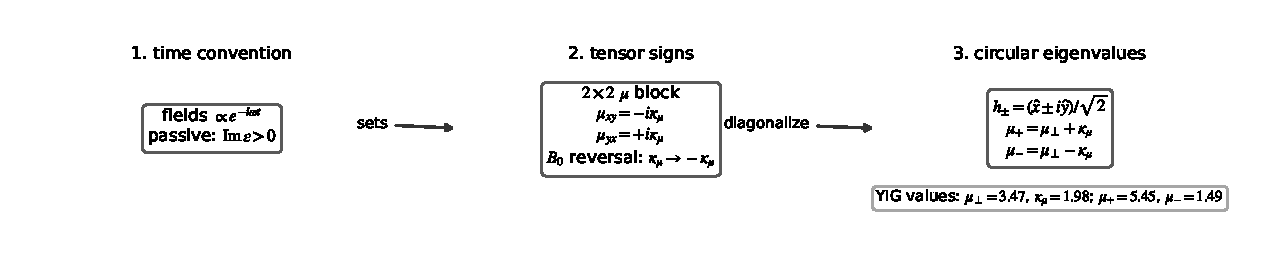
\includegraphics[width=0.96\textwidth]{figures/fig_appD_polder_sign_conventions.pdf}
  \caption{Material-tensor signs under the convention used throughout
  this monograph.  With fields proportional to $\ee^{-\ii\omega t}$,
  passive loss has $\operatorname{Im}\varepsilon>0$.  For a ferrite
  biased along $+\hat z$, the Polder tensor has the gyrotropic entries
  shown in the middle panel; reversing the bias flips $\kappa_\mu$.
    In the circular basis the eigenvalues are
    $\mu_+=\mu_\perp-\kappa_\mu$ (right-circular) and
    $\mu_-=\mu_\perp+\kappa_\mu$ (left-circular).  For the verified
    YIG parameters, $\mu_+=1.49$ and $\mu_-=5.45$.}
  \label{fig:appD-polder-sign-conventions}
\end{figure}


\section{Bianisotropic tensors}
\label{sec:appD-bianisotropic}

Bianisotropic media couple electric and magnetic fields \cite{slobozhanyuk2015observation}:
\begin{equation}\label{eq:appD-bianisotropic-expanded}
  \Dfield=\varepsilon_0\epst\Efield+\clight^{-1}\xit\Hfield\,,
  \qquad
  \Bfield=\clight^{-1}\zetat\Efield+\mu_0\mut\Hfield\,.
\end{equation}
Important special cases include:
\begin{enumerate}[label=(\roman*)]
  \item \textbf{Chiral media:} $\xit=\ii\chi\mathbf{I}$,
    $\zetat=-\ii\chi\mathbf{I}$ for reciprocal optical activity.
  \item \textbf{Tellegen media:} $\xit=\zetat=\chi_T\mathbf{I}$,
    which break time reversal and reciprocity.
  \item \textbf{Omega media:} antisymmetric magneto-electric coupling
    used in metamaterial realisations of pseudospin photonics.
\end{enumerate}
Bianisotropy is central to reciprocal photonic topological insulators,
where it couples TE and TM sectors in a controlled way \cite{khanikaev2013photonic}.

\section{Dispersive energy metric}
\label{sec:appD-energy-metric}

For a lossless but dispersive material, the correct energy inner product
uses the Brillouin energy density rather than the instantaneous field
energy \cite{gangaraj2016berry,silveirinha2016bulk}.  The dispersive
energy metric is
\begin{equation}\label{eq:appD-Mg}
  \Mgmat(\omega)=\pderiv{}{\omega}\bigl[\omega\Mmat(\omega)\bigr]
  =\Mmat(\omega)+\omega\pderiv{\Mmat}{\omega}\,.
\end{equation}
This formula applies block by block: the electric block is
$\varepsilon_0\,\partial_\omega(\omega\epst)$, the magnetic block is
$\mu_0\,\partial_\omega(\omega\mut)$, and the cross-coupling blocks
follow similarly.

\subsection{Physical origin}
\label{sec:appD-Mg-physical}

The extra term $\omega\,\partial_\omega\Mmat$ accounts for the energy
stored in the internal degrees of freedom of the medium---bound
electrons for a dielectric, precessing spins for a ferrite.  When the
field oscillates at frequency $\omega$, these internal oscillators
respond with an amplitude that depends on $\omega$; the total
time-averaged energy density is the sum of the vacuum-field energy and
the oscillator energy.  Brillouin showed that for a lossless dispersive
medium the result is exactly $\frac{1}{4}\emfield^\dagger\Mgmat\,\emfield$
\cite{gangaraj2016berry}.

\subsection{Positivity from passivity}
\label{sec:appD-Mg-positivity}

For the electromagnetic inner product and Berry connection to be
well-defined, the energy metric $\Mgmat$ must be positive definite.
This is guaranteed by passivity: a lossless medium that does not
spontaneously emit energy must store a non-negative energy density
for every nonzero field configuration.

More precisely, consider a quasi-monochromatic wave packet centred at
frequency $\omega$ with slowly varying envelope $\mathbf{a}(t)$.  The
time-averaged energy density is
\begin{equation}\label{eq:appD-energy-density}
  \langle u\rangle
  = \frac{1}{4}\,\mathbf{a}^\dagger\,
  \pderiv{}{\omega}\bigl[\omega\Mmat(\omega)\bigr]\,\mathbf{a}
  = \frac{1}{4}\,\mathbf{a}^\dagger\,\Mgmat(\omega)\,\mathbf{a}\,.
\end{equation}
Passivity requires $\langle u\rangle\geq 0$ for all $\mathbf{a}\neq 0$,
hence $\Mgmat(\omega)\geq 0$.  Strict positivity ($\Mgmat>0$) holds
at frequencies away from material resonances, where $\Mmat(\omega)$ is
smooth and the medium is transparent.

\section{Polder tensor: detailed derivation}
\label{sec:appD-polder-detailed}

For the Polder ferrite, the dispersive derivatives are
\cite{gangaraj2016berry} strict positivity of $\Mgmat$ can be verified
explicitly.  The circular-basis eigenvalues of the magnetic block are
$\mu_{g,\pm}=\partial_\omega(\omega\mu_\pm)$, with $\mu_\pm=\mu_\perp\mp\kappa_\mu$.
Since $\mu_+=1+\omega_m/(\omega_0+\omega)$ and
$\mu_-=1+\omega_m/(\omega_0-\omega)$, differentiation gives
\begin{equation}\label{eq:appD-Mg-ferrite-eigenvalues}
  \mu_{g,\pm}
  = 1 + \frac{\omega_m\,\omega_0}{(\omega_0\pm\omega)^2}\,.
\end{equation}
Both eigenvalues are manifestly positive for $\omega<\omega_0$ (below
ferromagnetic resonance), confirming that the energy metric is positive
definite in the operating range of gyromagnetic photonic crystals.

\subsection{Role in the Berry connection}
\label{sec:appD-Mg-berry}

The Berry connection of a photonic band is defined using the
$\Mgmat$-weighted inner product \cite{gangaraj2016berry}:
\begin{equation}\label{eq:appD-berry-Mg}
  \Aberry_{n,\alpha}
  = \ii\int_\Omega
  \mathbf{u}_{n\kvec}^\dagger\,\Mgmat(\omega_n)\,
  \nabla_{k_\alpha}\mathbf{u}_{n\kvec}\,\dd^d r\,.
\end{equation}
If one uses the bare material matrix $\Mmat$ instead of $\Mgmat$, the
resulting Berry connection is not gauge-invariant under frequency
relabelling, and the Chern number may depend on the choice of
normalisation.  The dispersive correction $\omega\,\partial_\omega\Mmat$
is therefore not a refinement but a necessity for any material with
frequency-dependent constitutive parameters \cite{silveirinha2016bulk}.
\begin{align}\label{eq:appD-polder-derivatives}
  \pderiv{\mu_\perp}{\omega}
  &=\frac{2\omega\omega_0\omega_m}{(\omega_0^2-\omega^2)^2}\,,\\
  \pderiv{\kappa_\mu}{\omega}
  &=\frac{\omega_m(\omega_0^2+\omega^2)}{(\omega_0^2-\omega^2)^2}\,.
\end{align}
Thus the transverse magnetic energy block is
\begin{equation}\label{eq:appD-Mg-polder}
  \mut_g=\begin{pmatrix}
    \mu_\perp+\omega\partial_\omega\mu_\perp &
      -\ii(\kappa_\mu+\omega\partial_\omega\kappa_\mu)&0\\
    \ii(\kappa_\mu+\omega\partial_\omega\kappa_\mu)&
      \mu_\perp+\omega\partial_\omega\mu_\perp&0\\
    0&0&1
  \end{pmatrix}\,.
\end{equation}
The eigenvalues in the circular basis are
\begin{equation}\label{eq:appD-Mg-circular}
  \mu_{g,\pm}=\mu_\perp+\omega\partial_\omega\mu_\perp
  \pm\bigl(\kappa_\mu+\omega\partial_\omega\kappa_\mu\bigr)\,.
\end{equation}
A passive stable ferrite away from resonance must have
$\mu_{g,+}>0$ and $\mu_{g,-}>0$.

\section{Drude and Lorentz response}
\label{sec:appD-drude-lorentz}

\subsection{Drude model}
\label{sec:appD-drude}

For free carriers,
\begin{equation}\label{eq:appD-drude}
  \varepsilon(\omega)=\varepsilon_\infty-
  \frac{\omega_p^2}{\omega(\omega+\ii\gamma_D)}\,
\end{equation}
The displayed formula above follows the convention and normalisation used in \cite{press2026photonic}.
With our $\ee^{-\ii\omega t}$ convention, $\gamma_D>0$ gives
absorption.  In the lossless limit $\gamma_D=0$,
\begin{equation}\label{eq:appD-drude-energy}
  \pderiv{}{\omega}\bigl[\omega\varepsilon(\omega)\bigr]
  =\varepsilon_\infty+\frac{\omega_p^2}{\omega^2}>0\,.
\end{equation}

\subsection{Lorentz oscillator}
\label{sec:appD-lorentz}

For a bound resonance,
\begin{equation}\label{eq:appD-lorentz}
  \varepsilon(\omega)=\varepsilon_\infty+
  \frac{f\omega_r^2}{\omega_r^2-\omega^2-\ii\gamma_L\omega}\,.
\end{equation}
In the lossless limit,
\begin{equation}\label{eq:appD-lorentz-energy}
  \partial_\omega[\omega\varepsilon(\omega)]
  =\varepsilon_\infty+f\omega_r^2\frac{\omega_r^2+\omega^2}{(\omega_r^2-\omega^2)^2}>0
\end{equation}
away from the material resonance.  This positivity is the oscillator
origin of the Brillouin energy formula.

\section{Useful constants and units}
\label{sec:appD-units}

\begin{center}
\begin{tabular}{lll}
  \toprule
  \textbf{Quantity} & \textbf{Symbol} & \textbf{SI value} \\
  \midrule
  Speed of light & $c$ & $2.99792458\times10^8\;\mathrm{m/s}$ \\
  Vacuum permittivity & $\varepsilon_0$ & $8.8541878128\times10^{-12}\;\mathrm{F/m}$ \\
  Vacuum permeability & $\mu_0$ & $1.25663706212\times10^{-6}\;\mathrm{H/m}$ \\
  Free-space impedance & $Z_0=\sqrt{\mu_0/\varepsilon_0}$ & $376.730313668\;\Omega$ \\
  Reduced Planck constant & $\hbar$ & $1.054571817\times10^{-34}\;\mathrm{J\,s}$ \\
  Electron charge & $e$ & $1.602176634\times10^{-19}\;\mathrm{C}$ \\
  Electron gyromagnetic ratio & $\gamma/(2\pi)$ & $28.025\;\mathrm{GHz/T}$ \\
  \bottomrule
\end{tabular}
\end{center}

\section{Checklist for translating sources}
\label{sec:appD-checklist}

Sources in topological photonics use a wide variety of sign conventions
\cite{ozawa2018topological,gangaraj2016berry}.  When using a formula
from another paper, check the following before
inserting it into this monograph:
\begin{enumerate}
  \item Does the paper use $\ee^{-\ii\omega t}$ or $\ee^{+\ii\omega t}$?
  \item Is the gyrotropic tensor written with $+\ii g$ or $-\ii g$ in
  the $xy$ component?
  \item Is the Berry connection defined as $+\ii\langle u|\nabla u\rangle$
  or $-\ii\langle u|\nabla u\rangle$?
  \item Is the inner product the bare $L^2$ product or the electromagnetic
  energy product with $\Mmat$ or $\Mgmat$?
  \item Is material dispersion ignored, approximated, or included through
  auxiliary oscillator variables?
  \item Are the quoted Chern numbers for individual bands, composite
  band groups, or gaps?
\end{enumerate}
Only after these convention checks should formulas be compared or cited.

\section{Kramers--Kronig relations and passivity} \cite{raman2010photonic,nittis2020equivalence}
\label{sec:appD-kramers-kronig}

\subsection{The dispersion relations}
\label{sec:appD-kk-derivation}

Any causal linear response function $\chi(\omega)$ satisfies the
Kramers--Kronig relations, which connect the real and imaginary parts:
\begin{align}
  \real\,\chi(\omega)
  &= \frac{1}{\pi}\,\mathrm{P.V.}\!\int_{-\infty}^{\infty}
  \frac{\imag\,\chi(\omega')}{\omega'-\omega}\,\dd\omega'\,,
  \label{eq:appD-kk-real}\\
  \imag\,\chi(\omega)
  &= -\frac{1}{\pi}\,\mathrm{P.V.}\!\int_{-\infty}^{\infty}
  \frac{\real\,\chi(\omega')}{\omega'-\omega}\,\dd\omega'\,.
  \label{eq:appD-kk-imag}
\end{align}
Here P.V.\ denotes the Cauchy principal value.  For the dielectric
permittivity $\varepsilon(\omega)=1+\chi_e(\omega)$, the Kramers--Kronig
relations guarantee that $\imag\,\varepsilon(\omega)>0$ for $\omega>0$
in a passive medium, and that the dispersive energy metric
$\Mgmat(\omega)=\partial_\omega[\omega\Mmat(\omega)]$ is positive
definite at all real frequencies outside the absorption bands
\cite{gangaraj2016berry,silveirinha2016bulk}.

\subsection{Passivity and the positive-definite metric}
\label{sec:appD-passivity}

A medium is passive if it does not provide energy to the field.
Mathematically, this requires that the power dissipated by any field
configuration is non-negative:
$\emfield^\dagger\,\imag[\omega\Mmat(\omega)]\,\emfield\geq 0$ for
all $\omega>0$ and all $\emfield$.  Combined with the Kramers--Kronig
relations, passivity implies \cite{gangaraj2016berry}
\begin{equation}\label{eq:appD-passivity}
  \Mgmat(\omega) = \frac{\partial[\omega\Mmat(\omega)]}{\partial\omega}
  \succ 0
  \quad\text{(positive definite)}
\end{equation}
at all real frequencies in the transparency windows (where
$\imag\,\Mmat\approx 0$).  This result, proved rigorously by
Silveirinha \cite{silveirinha2016bulk}, is the foundation for the
Hermitian structure of the photonic eigenproblem and the well-definedness
of the Chern number.

\section{Worked examples of sign-convention translation}
\label{sec:appD-worked-examples}

\subsection{Example 1: Haldane--Raghu to this book}
\label{sec:appD-example-haldane}

Haldane and Raghu \cite{haldane2008possible} use the convention
$\ee^{+\ii\omega t}$ for the time dependence.  In their notation,
the gyrotropic permittivity tensor has $+\ii g$ in the off-diagonal
position.  Translating to this book's convention ($\ee^{-\ii\omega t}$),
the gyrotropic coupling changes sign: $+\ii g\to -\ii g$.  The Chern
numbers are unaffected because the sign change affects both the
Hamiltonian and the inner product symmetrically.

\subsection{Example 2: Gangaraj--Silveirinha--Hanson to this book}
\label{sec:appD-example-gangaraj}

Gangaraj et~al.\ \cite{gangaraj2016berry} use $\ee^{-\ii\omega t}$
(same as this book) and define the Berry connection as
$\mathcal{A}_n=\ii\langle\emfield_n|\Mmat|\nabla_\kvec\emfield_n\rangle$,
consistent with our convention.  Their material matrix uses
$\Mmat=\diag(\varepsilon_0\epst,\mu_0\mut)$, which matches our
definition.  Formulas from this source can be used directly without
sign changes.

\section{Summary of convention choices in this book}
\label{sec:appD-convention-summary}

For reference, the complete set of convention choices used throughout
this monograph is collected here \cite{ozawa2018topological}:
\begin{center}
\begin{tabular}{ll}
  \toprule
  Convention & Choice \\
  \midrule
  Time dependence & $\ee^{-\ii\omega t}$ \\
  Gyrotropic off-diagonal & $-\ii\kappa_\mu$ (upper off-diagonal) \\
  Berry connection & $\mathcal{A}_n=\ii\eip{u_n}{\nabla_\kvec u_n}$ \\
  Inner product & $\eip{f_1}{f_2}=\int f_1^\dagger\Mmat\,f_2\,\dd V$ \\
  Dispersive metric & $\Mgmat=\partial_\omega[\omega\Mmat(\omega)]$ \\
  Chern number & $\Chern_n=\frac{1}{2\pi}\int_{\mathrm{BZ}}
    \mathcal{F}_n\,\dd^2 k$ \\
  Bloch convention & $\emfield_\kvec(\rvec)
    =\ee^{\ii\kvec\cdot\rvec}\mathbf{u}_\kvec(\rvec)$ \\
  Peierls phase & rightward hopping carries $+\phi$ \\
  \bottomrule
\end{tabular}
\end{center}

\section{Magneto-optical tensors for specific materials}
\label{sec:appD-specific-materials}

\subsection{Yttrium iron garnet (YIG)}
\label{sec:appD-yig-parameters}

YIG ($\mathrm{Y_3Fe_5O_{12}}$) is the standard material for microwave
topological photonics.  At a bias field $B_0=0.2\;\mathrm{T}$ and
frequency $f=4.5\;\mathrm{GHz}$, the Polder parameters are
\cite{ozawa2018topological,nature2026observation}:
\begin{center}
\begin{tabular}{ll}
  \toprule
  Parameter & Value \\
  \midrule
  Saturation magnetisation $4\pi M_s$ & $1780\;\mathrm{G}$ \\
  Gyromagnetic ratio $\gamma/(2\pi)$ & $28.0\;\mathrm{GHz/T}$ \\
  Resonance frequency $\omega_0/(2\pi)$ & $5.6\;\mathrm{GHz}$ \\
  Perpendicular permeability $\mu_\perp$ & $3.47$ \\
  Gyrotropic coupling $\kappa_\mu$ & $1.98$ \\
  Dielectric constant $\varepsilon_r$ & $15.0$ \\
  Gyrotropic ratio $\kappa_\mu/\mu_\perp$ & $0.57$ \\
  \bottomrule
\end{tabular}
\end{center}
The large gyrotropic ratio makes YIG the ideal material for
demonstrating Chern-insulator physics with wide topological gaps.

\subsection{Indium antimonide (InSb)}
\label{sec:appD-insb}

InSb is a narrow-gap semiconductor with strong magneto-plasma effects
at terahertz frequencies.  Under a magnetic field $B_0=0.3\;\mathrm{T}$
at $f=1\;\mathrm{THz}$, the relevant parameters are
\cite{price2022roadmap}:
\begin{center}
\begin{tabular}{ll}
  \toprule
  Parameter & Value \\
  \midrule
  Plasma frequency $\omega_p/(2\pi)$ & $2.0\;\mathrm{THz}$ \\
  Cyclotron frequency $\omega_c/(2\pi)$ & $0.5\;\mathrm{THz}$ \\
  Perpendicular permittivity $\varepsilon_\perp$ & $-3.0$ \\
  Gyrotropic coupling $\kappa_\varepsilon$ & $0.75$ \\
  Gyrotropic ratio $|\kappa_\varepsilon/\varepsilon_\perp|$ & $0.25$ \\
  \bottomrule
\end{tabular}
\end{center}
The negative perpendicular permittivity indicates operation above the
plasma frequency, where the material supports propagating modes with
strong gyrotropic splitting.

\subsection{Bismuth-substituted YIG (Bi:YIG)}
\label{sec:appD-biyig}

Bi:YIG ($\mathrm{Bi_xY_{3-x}Fe_5O_{12}}$) provides enhanced Faraday
rotation at near-infrared wavelengths compared to undoped YIG, but the
gyrotropic ratio remains small.  At $\lambda=1.55\;\mu\mathrm{m}$,
the off-diagonal permittivity is
$\kappa_\varepsilon\sim 10^{-2}$, giving a Faraday rotation of about
$0.5\;\mathrm{deg}/\mu\mathrm{m}$.  This is too weak for practical topological
gaps but sufficient for proof-of-concept magneto-optical devices
\cite{ozawa2018topological}.


\section{Experimental material parameters for topological photonics}
\label{sec:appD-experimental-params}

This section collects the material parameters used in the principal
experimental demonstrations discussed in this book, providing a
single reference for numerical computations and design.

\subsection{Yttrium iron garnet (YIG) at microwave frequencies}
\label{sec:appD-yig-params}

YIG is the standard material for microwave Chern insulators
(Chapter~\ref{ch:microwave-crystal}).  At saturation magnetisation
$M_s=1780\;\mathrm{G}$ and applied field $B_0=0.20\;\mathrm{T}$:
\begin{center}
\begin{tabular}{ll}
  \toprule
  Parameter & Value \\
  \midrule
  $\varepsilon_r$ & 15 \\
  $\omega_0/(2\pi)$ & 5.6\;GHz \\
  $\omega_m/(2\pi)$ & 4.9\;GHz \\
  $\mu_\perp$ & 3.47 \\
  $\kappa_\mu$ & 1.98 \\
  $\mu_\pm=\mu_\perp\mp\kappa_\mu$ & 1.49, 5.45 \\
  FMR linewidth $\Delta H$ & $\approx 0.3$\;Oe \\
  $\tan\delta_m$ & $\approx 3\times 10^{-4}$ \\
  \bottomrule
\end{tabular}
\end{center}
These parameters correspond to the Polder permeability tensor
\eqref{eq:appD-mu-polder} with saturation magnetisation along
$\hat{z}$ \cite{nature2026observation,skirlo2015experimental}.

\subsection{Silicon for valley and pseudospin designs}
\label{sec:appD-silicon-params}

Silicon is the dominant material for reciprocal topological photonic
designs at telecommunications wavelengths:
\begin{center}
\begin{tabular}{ll}
  \toprule
  Parameter & Value \\
  \midrule
  $\varepsilon_r$ at $\lambda=1.55\;\mu\mathrm{m}$ & 11.7 \\
  Refractive index $n$ & 3.42 \\
  Absorption $\alpha$ & $<0.1\;\mathrm{dB/cm}$ \\
  Thermo-optic $\dd n/\dd T$ & $1.86\times 10^{-4}\;\mathrm{K}^{-1}$ \\
  Kerr coefficient $n_2$ & $4.5\times 10^{-18}\;\mathrm{m}^2/\mathrm{W}$ \\
  \bottomrule
\end{tabular}
\end{center}
The negligible absorption and high refractive index make silicon ideal
for valley photonic crystals
(Chapter~\ref{ch:valleys}) and Wu--Hu pseudospin designs
(Chapter~\ref{ch:reciprocal-designs})
\cite{ma2016all,ozawa2018topological}.

\subsection{Fused silica for Floquet waveguide arrays}
\label{sec:appD-silica-params}

Fused silica is the substrate for laser-written waveguide arrays
used in Floquet topological experiments
(Chapter~\ref{ch:floquet}):
\begin{center}
\begin{tabular}{ll}
  \toprule
  Parameter & Value \\
  \midrule
  $n_0$ at $\lambda=633\;\mathrm{nm}$ & 1.457 \\
  Waveguide $\Delta n$ & $\approx 6\times 10^{-4}$ \\
  Propagation loss & $\approx 0.5\;\mathrm{dB/cm}$ \\
  Mode diameter & $\approx 10\;\mu\mathrm{m}$ \\
  \bottomrule
\end{tabular}
\end{center}
The low index contrast produces weakly guided modes with large
evanescent tails, enabling controllable inter-waveguide coupling at
separations of $d\approx 20$--$30\;\mu\mathrm{m}$
\cite{rechtsman2013photonica}.


\section{Sign-convention translation guide}
\label{sec:appD-sign-translation}

Different communities use different time-harmonic conventions, and
translating results between conventions is a frequent source of error
in topological photonics.  This section provides explicit translation
rules.

\subsection{Mapping between the two time-harmonic conventions}
\label{sec:appD-mapping}

Let quantities with a tilde denote the $\ee^{+\ii\omega t}$ convention.
The mapping is:
\begin{align}\label{eq:appD-convention-map}
  \tilde{\varepsilon}_{ij} &= \varepsilon_{ij}^*\,,
  &\tilde{\mu}_{ij} &= \mu_{ij}^*\,,\notag\\
  \tilde{\xi}_{ij} &= -\zeta_{ij}^*\,,
  &\tilde{\zeta}_{ij} &= -\xi_{ij}^*\,,\notag\\
  \tilde{\kappa}_\mu &= -\kappa_\mu^*\,,
  &\tilde{\kappa}_\varepsilon &= -\kappa_\varepsilon^*\,.
\end{align}
For lossless media where all tensor elements are real, the mapping
reduces to sign flips of the off-diagonal gyrotropic elements:
$\tilde{\kappa}_\mu=-\kappa_\mu$ and
$\tilde{\kappa}_\varepsilon=-\kappa_\varepsilon$.

\subsection{Practical examples}
\label{sec:appD-translation-examples}

\paragraph{YIG at 4.5\;GHz.}
In this book ($\ee^{-\ii\omega t}$): $\mu_\perp=3.47$,
$\kappa_\mu=+1.98$.  In the condensed-matter convention
($\ee^{+\ii\omega t}$): $\tilde{\mu}_\perp=3.47$,
$\tilde{\kappa}_\mu=-1.98$.  The Chern number is convention-independent:
$\Chern=+1$ in both cases, because both the Berry connection and the
integration orientation transform consistently.

\paragraph{Haldane--Raghu perturbation.}
Haldane and Raghu (2008) use $\ee^{+\ii\omega t}$, so their
gyrotropic parameter $\eta$ has the opposite sign relative to ours.
When importing their Dirac-mass formula
$m\propto\eta\langle u_1|\delta\varepsilon|u_2\rangle$, the sign of
$\eta$ must be flipped to match the $\ee^{-\ii\omega t}$ inner
product used in this book \cite{haldane2008possible,gangaraj2016berry}.

\paragraph{Bender--Boettcher PT symmetry.}
The original PT-symmetry literature uses $\ee^{+\ii\omega t}$, where
a PT-symmetric potential satisfies $V^*(-x)=V(x)$.  In our convention,
the same condition reads $V(-x)=V^*(x)$---i.e.\ the real part is even
and the imaginary part is odd, with gain ($\imag\varepsilon<0$)
and loss ($\imag\varepsilon>0$) interchanged relative to the
$\ee^{+\ii\omega t}$ literature \cite{bender1998real,guo2009observation}.

\section{Passivity, causality, and the Kramers--Kronig connection}
\label{sec:appD-passivity-causality}

The sign convention for absorption is not arbitrary: it is fixed by
the requirement that the material response be causal and passive.

For a causal, passive material with the $\ee^{-\ii\omega t}$ convention,
the permittivity $\varepsilon(\omega)$ is analytic in the lower half
of the complex $\omega$-plane, and the Kramers--Kronig relations
connect the real and imaginary parts:
\begin{align}\label{eq:appD-kk-causal}
  \operatorname{Re}\varepsilon(\omega)
  &= 1+\frac{2}{\pi}\,\mathcal{P}\!\int_0^\infty
  \frac{\omega'\,\operatorname{Im}\varepsilon(\omega')}
  {\omega'^2-\omega^2}\,\dd\omega'\,,\notag\\
  \operatorname{Im}\varepsilon(\omega)
  &= -\frac{2\omega}{\pi}\,\mathcal{P}\!\int_0^\infty
  \frac{\operatorname{Re}\varepsilon(\omega')-1}
  {\omega'^2-\omega^2}\,\dd\omega'\,.
\end{align}
Passivity requires that the power dissipated by any field distribution
be non-negative:
$\frac{1}{2}\omega\,\operatorname{Im}\varepsilon(\omega)\geq 0$
for all $\omega>0$.  Since $\omega>0$, this implies
$\operatorname{Im}\varepsilon(\omega)\geq 0$ for passive media,
confirming the sign convention used throughout this book
\cite{silveirinha2016bulk,ozawa2018topological}.

For active (gain) media, $\operatorname{Im}\varepsilon(\omega)<0$
in the amplifying frequency range, and the Kramers--Kronig relations
remain valid but the passivity condition is violated.  This is the
physical basis for the gain/loss classification used in
Chapter~\ref{ch:non-hermitian}.


\section{Kramers--Kronig relations and causality constraints}
\label{sec:appD-kramers-kronig-detail}

The frequency dependence of the material tensors is not arbitrary: it
is constrained by causality through the Kramers--Kronig relations.
These relations connect the real and imaginary parts of any causal
response function and provide important consistency checks for
material models used in topological photonics simulations.

\subsection{Derivation from causality}
\label{sec:appD-kk-causality-derivation}

A linear, time-invariant, causal response function $\chi(\omega)$
(e.g.\ the electric susceptibility $\varepsilon(\omega)-1$) is
analytic in the upper half of the complex frequency plane.  By
applying Cauchy's integral theorem to a contour that closes in the
upper half-plane, one obtains the Kramers--Kronig relations
\cite{raman2010photonic,nittis2020equivalence}:
\begin{align}
  \mathrm{Re}\,\chi(\omega) &= \frac{1}{\pi}\,
  \mathrm{P.V.}\!\int_{-\infty}^{\infty}
  \frac{\mathrm{Im}\,\chi(\omega')}{\omega'-\omega}\,\dd\omega'\,,
  \label{eq:appD-kk-real-causality}\\
  \mathrm{Im}\,\chi(\omega) &= -\frac{1}{\pi}\,
  \mathrm{P.V.}\!\int_{-\infty}^{\infty}
  \frac{\mathrm{Re}\,\chi(\omega')}{\omega'-\omega}\,\dd\omega'\,,
  \label{eq:appD-kk-imag-causality}
\end{align}
where P.V.\ denotes the Cauchy principal value.

\subsection{Sum rules for the gyrotropic response}
\label{sec:appD-sum-rules}

For the gyrotropic permeability $\kappa_\mu(\omega)$ of a ferrite
(Section~\ref{sec:appD-polder-detailed}), the Kramers--Kronig relations imply
a sum rule:
\begin{equation}\label{eq:appD-kappa-sum-rule}
  \int_0^\infty \omega\,\mathrm{Im}\,\kappa_\mu(\omega)\,\dd\omega
  = \frac{\pi}{2}\,\omega_M\,\omega_0\,,
\end{equation}
where $\omega_M=\gamma\mu_0 M_s$ and $\omega_0=\gamma\mu_0 H_0$ are
the magnetisation and precession frequencies.  This sum rule provides
a useful check on the Polder model: any deviation indicates that the
model is being used outside its range of validity
\cite{nature2026observation,gangaraj2016berry}.

\subsection{Implications for passivity and topological gaps}
\label{sec:appD-passivity-topology}

The Kramers--Kronig relations also constrain the size of the
topological gap.  Because the gyrotropic coupling $\kappa_\mu$ must
satisfy the sum rule, increasing $\kappa_\mu$ at one frequency
necessarily decreases it at other frequencies.  This means that the
topological gap width is bounded by the total oscillator strength
available in the gyrotropic response.

For ferrites, the oscillator strength is concentrated near the
ferromagnetic resonance, so the largest topological gaps occur at
frequencies just below $\omega_0$.  Moving to higher frequencies
(e.g.\ optical) reduces the available gyrotropic coupling and
narrows the gap, as discussed in
Chapter~\ref{ch:breaking-tr} \cite{zhao2020first,price2022roadmap}.

\section{Material parameter tables for topological photonics}
\label{sec:appD-parameter-tables}

\subsection{Common microwave materials}
\label{sec:appD-microwave-table}

Table~\ref{tab:appD-microwave} lists the key material parameters for
the most commonly used microwave-frequency topological photonic
materials.

\begin{table}[htbp]
\centering
\caption{Material parameters for microwave topological photonics.
All values at room temperature; YIG parameters at $B_0=0.20\;\mathrm{T}$,
$f=4.5\;\mathrm{GHz}$.}
\label{tab:appD-microwave}
\begin{tabular}{lcccc}
\hline
Material & $\varepsilon_r$ & $\mu_\perp$ & $\kappa_\mu/\mu_\perp$
& Topological gap \\
\hline
YIG (single crystal) & 15.0 & 3.47 & 0.57 & $\sim 3\%$ \\
BaFe$_{12}$O$_{19}$ & 18.0 & 1.8 & 0.35 & $\sim 1.5\%$ \\
Li ferrite & 14.5 & 2.5 & 0.45 & $\sim 2\%$ \\
\hline
\end{tabular}
\end{table}

\subsection{Common optical and infrared materials}
\label{sec:appD-optical-table}

Table~\ref{tab:appD-optical} lists the parameters for optical-frequency
topological photonic crystals, where the gyrotropic response is replaced
by geometric or Floquet engineering.

\begin{table}[htbp]
\centering
\caption{Material parameters for optical/infrared topological photonics.}
\label{tab:appD-optical}
\begin{tabular}{lcccc}
\hline
Material & $\varepsilon_r$ & Platform & Mechanism
& Topological gap \\
\hline
Silicon ($\lambda=1550\;\mathrm{nm}$) & 12.1
& Valley PhC & Inversion breaking & $\sim 5\%$ \\
SiN ($\lambda=780\;\mathrm{nm}$) & 4.0
& Ring resonator & Synthetic gauge & $\sim 1\%$ \\
Fused silica (fs-written) & 1.45
& Floquet waveguide & Helix modulation & $\sim 2\%$ \\
Ce:YIG ($\lambda=1550\;\mathrm{nm}$) & 5.4
& Magneto-optical & Faraday effect & $\sim 0.01\%$ \\
\hline
\end{tabular}
\end{table}

These tables illustrate the fundamental trade-off in topological
photonics: microwave materials provide the largest topological gaps
through genuine time-reversal breaking, while optical materials offer
compatibility with integrated photonic platforms at the cost of either
weaker topological protection (valley and Floquet mechanisms) or
extremely narrow gaps (magneto-optical route)
\cite{ozawa2018topological,he2019silicon,rechtsman2013photonic,
price2022roadmap}.


% ======================================================================
\backmatter

% ---- Bibliography ----
\printbibliography[heading=bibintoc,title={References}]

% ---- Index ----
\printindex

\end{document}
